\par In this chapter, comparison of the new COSY routines will be benchmarked against both ICOOL and G4Beamline for pencil beams through. Moreover, both validation against past experiments and predictions of future experiments will be shown.

\Section{Benchmark Against Other Codes}\label{sec:benchmark}

This section shows the comparison of the new COSY routines with those of two other codes, ICOOL \cite{icool} and G4Beamline \cite{g4bl}. The comparisons are done over both the momentum range of cooling channels (100, 200, 300, and 400 MeV/$c$) and various absorber lengths (1, 10, and 100 mm). These simulations were performed using a pencil beam of the aforementioned momenta through liquid hydrogen.

\newpage

\iftrue % to save on time

\begin{center}
\tikzset{every picture/.style={scale=0.5,every picture/.style={}}}
\noindent
\frame{      \pgfdeclareplotmark{cross} {
\pgfpathmoveto{\pgfpoint{-0.3\pgfplotmarksize}{\pgfplotmarksize}}
\pgfpathlineto{\pgfpoint{+0.3\pgfplotmarksize}{\pgfplotmarksize}}
\pgfpathlineto{\pgfpoint{+0.3\pgfplotmarksize}{0.3\pgfplotmarksize}}
\pgfpathlineto{\pgfpoint{+1\pgfplotmarksize}{0.3\pgfplotmarksize}}
\pgfpathlineto{\pgfpoint{+1\pgfplotmarksize}{-0.3\pgfplotmarksize}}
\pgfpathlineto{\pgfpoint{+0.3\pgfplotmarksize}{-0.3\pgfplotmarksize}}
\pgfpathlineto{\pgfpoint{+0.3\pgfplotmarksize}{-1.\pgfplotmarksize}}
\pgfpathlineto{\pgfpoint{-0.3\pgfplotmarksize}{-1.\pgfplotmarksize}}
\pgfpathlineto{\pgfpoint{-0.3\pgfplotmarksize}{-0.3\pgfplotmarksize}}
\pgfpathlineto{\pgfpoint{-1.\pgfplotmarksize}{-0.3\pgfplotmarksize}}
\pgfpathlineto{\pgfpoint{-1.\pgfplotmarksize}{0.3\pgfplotmarksize}}
\pgfpathlineto{\pgfpoint{-0.3\pgfplotmarksize}{0.3\pgfplotmarksize}}
\pgfpathclose
\pgfusepathqstroke
}
\pgfdeclareplotmark{cross*} {
\pgfpathmoveto{\pgfpoint{-0.3\pgfplotmarksize}{\pgfplotmarksize}}
\pgfpathlineto{\pgfpoint{+0.3\pgfplotmarksize}{\pgfplotmarksize}}
\pgfpathlineto{\pgfpoint{+0.3\pgfplotmarksize}{0.3\pgfplotmarksize}}
\pgfpathlineto{\pgfpoint{+1\pgfplotmarksize}{0.3\pgfplotmarksize}}
\pgfpathlineto{\pgfpoint{+1\pgfplotmarksize}{-0.3\pgfplotmarksize}}
\pgfpathlineto{\pgfpoint{+0.3\pgfplotmarksize}{-0.3\pgfplotmarksize}}
\pgfpathlineto{\pgfpoint{+0.3\pgfplotmarksize}{-1.\pgfplotmarksize}}
\pgfpathlineto{\pgfpoint{-0.3\pgfplotmarksize}{-1.\pgfplotmarksize}}
\pgfpathlineto{\pgfpoint{-0.3\pgfplotmarksize}{-0.3\pgfplotmarksize}}
\pgfpathlineto{\pgfpoint{-1.\pgfplotmarksize}{-0.3\pgfplotmarksize}}
\pgfpathlineto{\pgfpoint{-1.\pgfplotmarksize}{0.3\pgfplotmarksize}}
\pgfpathlineto{\pgfpoint{-0.3\pgfplotmarksize}{0.3\pgfplotmarksize}}
\pgfpathclose
\pgfusepathqfillstroke
}
\pgfdeclareplotmark{newstar} {
\pgfpathmoveto{\pgfqpoint{0pt}{\pgfplotmarksize}}
\pgfpathlineto{\pgfqpointpolar{44}{0.5\pgfplotmarksize}}
\pgfpathlineto{\pgfqpointpolar{18}{\pgfplotmarksize}}
\pgfpathlineto{\pgfqpointpolar{-20}{0.5\pgfplotmarksize}}
\pgfpathlineto{\pgfqpointpolar{-54}{\pgfplotmarksize}}
\pgfpathlineto{\pgfqpointpolar{-90}{0.5\pgfplotmarksize}}
\pgfpathlineto{\pgfqpointpolar{234}{\pgfplotmarksize}}
\pgfpathlineto{\pgfqpointpolar{198}{0.5\pgfplotmarksize}}
\pgfpathlineto{\pgfqpointpolar{162}{\pgfplotmarksize}}
\pgfpathlineto{\pgfqpointpolar{134}{0.5\pgfplotmarksize}}
\pgfpathclose
\pgfusepathqstroke
}
\pgfdeclareplotmark{newstar*} {
\pgfpathmoveto{\pgfqpoint{0pt}{\pgfplotmarksize}}
\pgfpathlineto{\pgfqpointpolar{44}{0.5\pgfplotmarksize}}
\pgfpathlineto{\pgfqpointpolar{18}{\pgfplotmarksize}}
\pgfpathlineto{\pgfqpointpolar{-20}{0.5\pgfplotmarksize}}
\pgfpathlineto{\pgfqpointpolar{-54}{\pgfplotmarksize}}
\pgfpathlineto{\pgfqpointpolar{-90}{0.5\pgfplotmarksize}}
\pgfpathlineto{\pgfqpointpolar{234}{\pgfplotmarksize}}
\pgfpathlineto{\pgfqpointpolar{198}{0.5\pgfplotmarksize}}
\pgfpathlineto{\pgfqpointpolar{162}{\pgfplotmarksize}}
\pgfpathlineto{\pgfqpointpolar{134}{0.5\pgfplotmarksize}}
\pgfpathclose
\pgfusepathqfillstroke
}
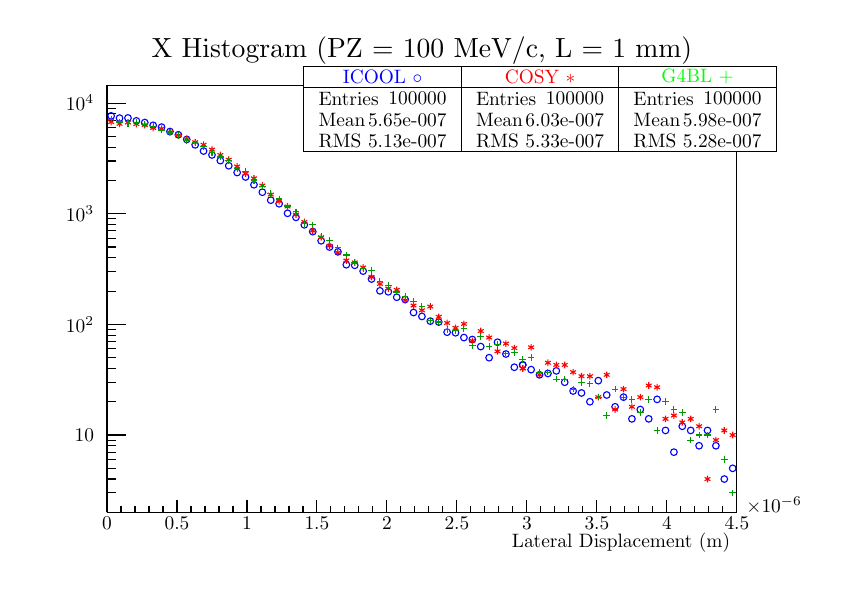
\begin{tikzpicture}
\definecolor{c}{rgb}{1,1,1};
\draw [color=c, fill=c] (0,0) rectangle (20,13.5632);
\draw [color=c, fill=c] (2,1.35632) rectangle (18,12.2069);
\definecolor{c}{rgb}{0,0,0};
\draw [c] (2,1.35632) -- (2,12.2069) -- (18,12.2069) -- (18,1.35632) -- (2,1.35632);
\definecolor{c}{rgb}{1,1,1};
\draw [color=c, fill=c] (2,1.35632) rectangle (18,12.2069);
\definecolor{c}{rgb}{0,0,0};
\draw [c] (2,1.35632) -- (2,12.2069) -- (18,12.2069) -- (18,1.35632) -- (2,1.35632);
\definecolor{c}{rgb}{0,0,1};
\foreach \P in
 {(2.10667,11.4269),(2.32,11.37),(2.53333,11.374),(2.74667,11.3003),(2.96,11.2572),(3.17333,11.1876),(3.38667,11.1414),(3.6,11.0291),(3.81333,10.9465),(4.02667,10.8281),(4.24,10.6912),(4.45333,10.534),(4.66667,10.4348),(4.88,10.2905),(5.09333,10.1602
),(5.30667,9.98813),(5.52,9.87429),(5.73333,9.67741),(5.94667,9.48782),(6.16,9.28556),(6.37333,9.19483),(6.58667,8.95212),(6.8,8.84998),(7.01333,8.65965),(7.22667,8.48653),(7.44,8.25512),(7.65333,8.0952),(7.86667,7.97472),(8.08,7.64586),(8.29333,7.63
166),(8.50667,7.48389),(8.72,7.28293),(8.93333,6.98297),(9.14667,6.95843),(9.36,6.82086),(9.57333,6.76408),(9.78667,6.43219),(10,6.33291),(10.2133,6.21348),(10.4267,6.19045),(10.64,5.93255),(10.8533,5.91811),(11.0667,5.79595),(11.28,5.7468),(11.4933,
5.56699),(11.7067,5.28492),(11.92,5.67802),(12.1333,5.37885),(12.3467,5.04272),(12.56,5.10085)}{\draw[mark options={color=c,fill=c},mark size=2.402402pt,mark=o] plot coordinates {\P};}
\foreach \P in
 {(12.56,5.10085),(12.7733,4.98168),(12.9867,4.84961),(13.2,4.88399),(13.4133,4.94998),(13.6267,4.66147),(13.84,4.43894),(14.0533,4.38912),(14.2667,4.1666),(14.48,4.70149),(14.6933,4.33718),(14.9067,4.03801),(15.12,4.28293),(15.3333,3.73128),(15.5467
,3.96825),(15.76,3.73128),(15.9733,4.22615),(16.1867,3.43695),(16.4,2.8853),(16.6133,3.54314),(16.8267,3.43695),(17.04,3.04828),(17.2533,3.43695),(17.4667,3.04828),(17.68,2.2023),(17.8933,2.47464)}{\draw[mark options={color=c,fill=c},mark
 size=2.402402pt,mark=o] plot coordinates {\P};}
\definecolor{c}{rgb}{1,1,1};
\draw [color=c, fill=c] (7,10.5115) rectangle (11,12.6816);
\definecolor{c}{rgb}{0,0,0};
\draw [c] (7,10.5115) -- (11,10.5115);
\draw [c] (11,10.5115) -- (11,12.6816);
\draw [c] (11,12.6816) -- (7,12.6816);
\draw [c] (7,12.6816) -- (7,10.5115);
\draw[color=blue](9,12.4103) node[scale=0.7, rotate=0]{ICOOL $\circ$};
\draw [c] (7,12.1391) -- (11,12.1391);
\draw [anchor= west] (7.2,11.8678) node[scale=0.6, rotate=0]{Entries };
\draw [anchor= east] (10.8,11.8678) node[scale=0.6, rotate=0]{ 100000};
\draw [anchor= west] (7.2,11.3253) node[scale=0.6, rotate=0]{Mean  };
\draw [anchor= east] (10.8,11.3253) node[scale=0.6, rotate=0]{ 5.65e-007};
\draw [anchor= west] (7.2,10.7828) node[scale=0.6, rotate=0]{RMS   };
\draw [anchor= east] (10.8,10.7828) node[scale=0.6, rotate=0]{ 5.13e-007};
\draw [c] (2,1.35632) -- (18,1.35632);
\draw [anchor= east] (18,0.596782) node[scale=0.7, rotate=0]{Lateral Displacement (m)};
\draw [c] (2,1.68184) -- (2,1.35632);
\draw [c] (2.35556,1.51908) -- (2.35556,1.35632);
\draw [c] (2.71111,1.51908) -- (2.71111,1.35632);
\draw [c] (3.06667,1.51908) -- (3.06667,1.35632);
\draw [c] (3.42222,1.51908) -- (3.42222,1.35632);
\draw [c] (3.77778,1.68184) -- (3.77778,1.35632);
\draw [c] (4.13333,1.51908) -- (4.13333,1.35632);
\draw [c] (4.48889,1.51908) -- (4.48889,1.35632);
\draw [c] (4.84444,1.51908) -- (4.84444,1.35632);
\draw [c] (5.2,1.51908) -- (5.2,1.35632);
\draw [c] (5.55556,1.68184) -- (5.55556,1.35632);
\draw [c] (5.91111,1.51908) -- (5.91111,1.35632);
\draw [c] (6.26667,1.51908) -- (6.26667,1.35632);
\draw [c] (6.62222,1.51908) -- (6.62222,1.35632);
\draw [c] (6.97778,1.51908) -- (6.97778,1.35632);
\draw [c] (7.33333,1.68184) -- (7.33333,1.35632);
\draw [c] (7.68889,1.51908) -- (7.68889,1.35632);
\draw [c] (8.04444,1.51908) -- (8.04444,1.35632);
\draw [c] (8.4,1.51908) -- (8.4,1.35632);
\draw [c] (8.75556,1.51908) -- (8.75556,1.35632);
\draw [c] (9.11111,1.68184) -- (9.11111,1.35632);
\draw [c] (9.46667,1.51908) -- (9.46667,1.35632);
\draw [c] (9.82222,1.51908) -- (9.82222,1.35632);
\draw [c] (10.1778,1.51908) -- (10.1778,1.35632);
\draw [c] (10.5333,1.51908) -- (10.5333,1.35632);
\draw [c] (10.8889,1.68184) -- (10.8889,1.35632);
\draw [c] (11.2444,1.51908) -- (11.2444,1.35632);
\draw [c] (11.6,1.51908) -- (11.6,1.35632);
\draw [c] (11.9556,1.51908) -- (11.9556,1.35632);
\draw [c] (12.3111,1.51908) -- (12.3111,1.35632);
\draw [c] (12.6667,1.68184) -- (12.6667,1.35632);
\draw [c] (13.0222,1.51908) -- (13.0222,1.35632);
\draw [c] (13.3778,1.51908) -- (13.3778,1.35632);
\draw [c] (13.7333,1.51908) -- (13.7333,1.35632);
\draw [c] (14.0889,1.51908) -- (14.0889,1.35632);
\draw [c] (14.4444,1.68184) -- (14.4444,1.35632);
\draw [c] (14.8,1.51908) -- (14.8,1.35632);
\draw [c] (15.1556,1.51908) -- (15.1556,1.35632);
\draw [c] (15.5111,1.51908) -- (15.5111,1.35632);
\draw [c] (15.8667,1.51908) -- (15.8667,1.35632);
\draw [c] (16.2222,1.68184) -- (16.2222,1.35632);
\draw [c] (16.5778,1.51908) -- (16.5778,1.35632);
\draw [c] (16.9333,1.51908) -- (16.9333,1.35632);
\draw [c] (17.2889,1.51908) -- (17.2889,1.35632);
\draw [c] (17.6444,1.51908) -- (17.6444,1.35632);
\draw [c] (18,1.68184) -- (18,1.35632);
\draw [c] (18,1.68184) -- (18,1.35632);
\draw [anchor=base] (2,0.908736) node[scale=0.7, rotate=0]{0};
\draw [anchor=base] (3.77778,0.908736) node[scale=0.7, rotate=0]{0.5};
\draw [anchor=base] (5.55556,0.908736) node[scale=0.7, rotate=0]{1};
\draw [anchor=base] (7.33333,0.908736) node[scale=0.7, rotate=0]{1.5};
\draw [anchor=base] (9.11111,0.908736) node[scale=0.7, rotate=0]{2};
\draw [anchor=base] (10.8889,0.908736) node[scale=0.7, rotate=0]{2.5};
\draw [anchor=base] (12.6667,0.908736) node[scale=0.7, rotate=0]{3};
\draw [anchor=base] (14.4444,0.908736) node[scale=0.7, rotate=0]{3.5};
\draw [anchor=base] (16.2222,0.908736) node[scale=0.7, rotate=0]{4};
\draw [anchor=base] (18,0.908736) node[scale=0.7, rotate=0]{4.5};
\draw [anchor=base west] (18.07,1.35632) node[scale=0.7, rotate=0]{$\times10^{-6}$};
\draw [c] (2,1.35632) -- (2,12.2069);
\draw [c] (2.24,1.85118) -- (2,1.85118);
\draw [c] (2.24,2.2023) -- (2,2.2023);
\draw [c] (2.24,2.47464) -- (2,2.47464);
\draw [c] (2.24,2.69716) -- (2,2.69716);
\draw [c] (2.24,2.8853) -- (2,2.8853);
\draw [c] (2.24,3.04828) -- (2,3.04828);
\draw [c] (2.24,3.19203) -- (2,3.19203);
\draw [c] (2.48,3.32062) -- (2,3.32062);
\draw [anchor= east] (1.844,3.32062) node[scale=0.7, rotate=0]{10};
\draw [c] (2.24,4.1666) -- (2,4.1666);
\draw [c] (2.24,4.66146) -- (2,4.66146);
\draw [c] (2.24,5.01258) -- (2,5.01258);
\draw [c] (2.24,5.28492) -- (2,5.28492);
\draw [c] (2.24,5.50744) -- (2,5.50744);
\draw [c] (2.24,5.69558) -- (2,5.69558);
\draw [c] (2.24,5.85856) -- (2,5.85856);
\draw [c] (2.24,6.00231) -- (2,6.00231);
\draw [c] (2.48,6.1309) -- (2,6.1309);
\draw [anchor= east] (1.844,6.1309) node[scale=0.7, rotate=0]{$10^{2}$};
\draw [c] (2.24,6.97688) -- (2,6.97688);
\draw [c] (2.24,7.47174) -- (2,7.47174);
\draw [c] (2.24,7.82286) -- (2,7.82286);
\draw [c] (2.24,8.0952) -- (2,8.0952);
\draw [c] (2.24,8.31772) -- (2,8.31772);
\draw [c] (2.24,8.50586) -- (2,8.50586);
\draw [c] (2.24,8.66884) -- (2,8.66884);
\draw [c] (2.24,8.81259) -- (2,8.81259);
\draw [c] (2.48,8.94118) -- (2,8.94118);
\draw [anchor= east] (1.844,8.94118) node[scale=0.7, rotate=0]{$10^{3}$};
\draw [c] (2.24,9.78716) -- (2,9.78716);
\draw [c] (2.24,10.282) -- (2,10.282);
\draw [c] (2.24,10.6331) -- (2,10.6331);
\draw [c] (2.24,10.9055) -- (2,10.9055);
\draw [c] (2.24,11.128) -- (2,11.128);
\draw [c] (2.24,11.3161) -- (2,11.3161);
\draw [c] (2.24,11.4791) -- (2,11.4791);
\draw [c] (2.24,11.6229) -- (2,11.6229);
\draw [c] (2.48,11.7515) -- (2,11.7515);
\draw [anchor= east] (1.844,11.7515) node[scale=0.7, rotate=0]{$10^{4}$};
\definecolor{c}{rgb}{1,1,1};
\draw [color=c, fill=c] (7,10.5115) rectangle (11,12.6816);
\definecolor{c}{rgb}{0,0,0};
\draw [c] (7,10.5115) -- (11,10.5115);
\draw [c] (11,10.5115) -- (11,12.6816);
\draw [c] (11,12.6816) -- (7,12.6816);
\draw [c] (7,12.6816) -- (7,10.5115);
\draw[color=blue](9,12.4103) node[scale=0.7, rotate=0]{ICOOL $\circ$};
\draw [c] (7,12.1391) -- (11,12.1391);
\draw [anchor= west] (7.2,11.8678) node[scale=0.7, rotate=0]{Entries };
\draw [anchor= east] (10.8,11.8678) node[scale=0.7, rotate=0]{ 100000};
\draw [anchor= west] (7.2,11.3253) node[scale=0.7, rotate=0]{Mean  };
\draw [anchor= east] (10.8,11.3253) node[scale=0.7, rotate=0]{ 5.65e-007};
\draw [anchor= west] (7.2,10.7828) node[scale=0.7, rotate=0]{RMS   };
\draw [anchor= east] (10.8,10.7828) node[scale=0.7, rotate=0]{ 5.13e-007};
\draw (10,13.0816) node[scale=1, rotate=0]{X Histogram (PZ = 100 MeV/c, L = 1 mm)};
\definecolor{c}{rgb}{1,0,0};
\foreach \P in
 {(2.10667,11.2696),(2.32,11.2244),(2.53333,11.2578),(2.74667,11.2187),(2.96,11.1939),(3.17333,11.1207),(3.38667,11.1015),(3.6,11.0107),(3.81333,10.9332),(4.02667,10.8408),(4.24,10.7578),(4.45333,10.6936),(4.66667,10.5702),(4.88,10.433),(5.09333,10.3
134),(5.30667,10.1407),(5.52,9.95986),(5.73333,9.83913),(5.94667,9.65789),(6.16,9.42788),(6.37333,9.25951),(6.58667,9.12443),(6.8,8.91901),(7.01333,8.73274),(7.22667,8.51282),(7.44,8.34389),(7.65333,8.12891),(7.86667,7.95297),(8.08,7.75381),(8.29333,
7.7044),(8.50667,7.57692),(8.72,7.33408),(8.93333,7.15802),(9.14667,7.04223),(9.36,7.00702),(9.57333,6.74209),(9.78667,6.60938),(10,6.4881),(10.2133,6.58439),(10.4267,6.32252),(10.64,6.16698),(10.8533,6.04233),(11.0667,6.14305),(11.28,5.7129),(11.493
3,5.96093),(11.7067,5.79595),(11.92,5.44484),(12.1333,5.64212),(12.3467,5.52762),(12.56,5.01258)}{\draw[mark options={color=c,fill=c},mark size=2.402402pt,mark=asterisk] plot coordinates {\P};}
\foreach \P in
 {(12.56,5.01258),(12.7733,5.54746),(12.9867,4.84961),(13.2,5.15633),(13.4133,5.10085),(13.6267,5.10085),(13.84,4.91743),(14.0533,4.81423),(14.2667,4.81423),(14.48,4.28293),(14.6933,4.84961),(14.9067,3.96825),(15.12,4.48681),(15.3333,4.03801),(15.546
7,4.28293),(15.76,4.57726),(15.9733,4.53288),(16.1867,3.73128),(16.4,3.81549),(16.6133,3.64084),(16.8267,3.73128),(17.04,3.54314),(17.2533,2.2023),(17.4667,3.19203),(17.68,3.43695),(17.8933,3.32062)}{\draw[mark options={color=c,fill=c},mark
 size=2.402402pt,mark=asterisk] plot coordinates {\P};}
\definecolor{c}{rgb}{1,1,1};
\draw [color=c, fill=c] (11,10.5115) rectangle (15,12.6816);
\definecolor{c}{rgb}{0,0,0};
\draw [c] (11,10.5115) -- (15,10.5115);
\draw [c] (15,10.5115) -- (15,12.6816);
\draw [c] (15,12.6816) -- (11,12.6816);
\draw [c] (11,12.6816) -- (11,10.5115);
\draw [color=red](13,12.4103) node[scale=0.7, rotate=0]{COSY $*$};
\draw [c] (11,12.1391) -- (15,12.1391);
\draw [anchor= west] (11.2,11.8678) node[scale=0.7, rotate=0]{Entries };
\draw [anchor= east] (14.8,11.8678) node[scale=0.7, rotate=0]{ 100000};
\draw [anchor= west] (11.2,11.3253) node[scale=0.7, rotate=0]{Mean  };
\draw [anchor= east] (14.8,11.3253) node[scale=0.7, rotate=0]{ 6.03e-007};
\draw [anchor= west] (11.2,10.7828) node[scale=0.7, rotate=0]{RMS   };
\draw [anchor= east] (14.8,10.7828) node[scale=0.7, rotate=0]{ 5.33e-007};
\definecolor{c}{rgb}{1,1,1};
\draw [color=c, fill=c] (11,10.5115) rectangle (15,12.6816);
\definecolor{c}{rgb}{0,0,0};
\draw [c] (11,10.5115) -- (15,10.5115);
\draw [c] (15,10.5115) -- (15,12.6816);
\draw [c] (15,12.6816) -- (11,12.6816);
\draw [c] (11,12.6816) -- (11,10.5115);
\draw [color=red](13,12.4103) node[scale=0.7, rotate=0]{COSY $*$};
\draw [c] (11,12.1391) -- (15,12.1391);
\draw [anchor= west] (11.2,11.8678) node[scale=0.7, rotate=0]{Entries };
\draw [anchor= east] (14.8,11.8678) node[scale=0.7, rotate=0]{ 100000};
\draw [anchor= west] (11.2,11.3253) node[scale=0.7, rotate=0]{Mean  };
\draw [anchor= east] (14.8,11.3253) node[scale=0.7, rotate=0]{ 6.03e-007};
\draw [anchor= west] (11.2,10.7828) node[scale=0.7, rotate=0]{RMS   };
\draw [anchor= east] (14.8,10.7828) node[scale=0.7, rotate=0]{ 5.33e-007};
\definecolor{c}{rgb}{0,0.6,0};
\foreach \P in
 {(2.10667,11.3272),(2.32,11.2721),(2.53333,11.2279),(2.74667,11.2539),(2.96,11.203),(3.17333,11.1609),(3.38667,11.0673),(3.6,11.0136),(3.81333,10.921),(4.02667,10.8082),(4.24,10.7522),(4.45333,10.6456),(4.66667,10.4943),(4.88,10.382),(5.09333,10.285
7),(5.30667,10.0956),(5.52,10.0066),(5.73333,9.77489),(5.94667,9.62836),(6.16,9.45382),(6.37333,9.31467),(6.58667,9.13801),(6.8,8.98787),(7.01333,8.69001),(7.22667,8.65657),(7.44,8.36755),(7.65333,8.25726),(7.86667,8.07303),(8.08,7.89397),(8.29333,7.
7044),(8.50667,7.53902),(8.72,7.50387),(8.93333,7.21957),(9.14667,7.12063),(9.36,6.95222),(9.57333,6.84149),(9.78667,6.71214),(10,6.59278),(10.2133,6.22483),(10.4267,6.19045),(10.64,6.00231),(10.8533,5.97488),(11.0667,6.02914),(11.28,5.58621),(11.493
3,5.81191),(11.7067,5.56699),(11.92,5.62377),(12.1333,5.40125),(12.3467,5.42324),(12.56,5.2351)}{\draw[mark options={color=c,fill=c},mark size=2.402402pt,mark=+] plot coordinates {\P};}
\foreach \P in
 {(12.56,5.2351),(12.7733,5.28492),(12.9867,4.91743),(13.2,4.91743),(13.4133,4.74023),(13.6267,4.74023),(13.84,4.48681),(14.0533,4.66147),(14.2667,4.62009),(14.48,4.28293),(14.6933,3.81549),(14.9067,4.48681),(15.12,4.28293),(15.3333,4.22615),(15.5467
,3.89426),(15.76,4.22615),(15.9733,3.43695),(16.1867,4.1666),(16.4,3.96825),(16.6133,3.89426),(16.8267,3.19203),(17.04,3.32062),(17.2533,3.32062),(17.4667,3.96825),(17.68,2.69717),(17.8933,1.85119)}{\draw[mark options={color=c,fill=c},mark
 size=2.402402pt,mark=+] plot coordinates {\P};}
\definecolor{c}{rgb}{1,1,1};
\draw [color=c, fill=c] (15,10.5115) rectangle (19,12.6816);
\definecolor{c}{rgb}{0,0,0};
\draw [c] (15,10.5115) -- (19,10.5115);
\draw [c] (19,10.5115) -- (19,12.6816);
\draw [c] (19,12.6816) -- (15,12.6816);
\draw [c] (15,12.6816) -- (15,10.5115);
\draw [color=green](17,12.4103) node[scale=0.7, rotate=0]{G4BL $+$};
\draw [c] (15,12.1391) -- (19,12.1391);
\draw [anchor= west] (15.2,11.8678) node[scale=0.7, rotate=0]{Entries };
\draw [anchor= east] (18.8,11.8678) node[scale=0.7, rotate=0]{ 100000};
\draw [anchor= west] (15.2,11.3253) node[scale=0.7, rotate=0]{Mean  };
\draw [anchor= east] (18.8,11.3253) node[scale=0.7, rotate=0]{ 5.98e-007};
\draw [anchor= west] (15.2,10.7828) node[scale=0.7, rotate=0]{RMS   };
\draw [anchor= east] (18.8,10.7828) node[scale=0.7, rotate=0]{ 5.28e-007};
\definecolor{c}{rgb}{1,1,1};
\draw [color=c, fill=c] (15,10.5115) rectangle (19,12.6816);
\definecolor{c}{rgb}{0,0,0};
\draw [c] (15,10.5115) -- (19,10.5115);
\draw [c] (19,10.5115) -- (19,12.6816);
\draw [c] (19,12.6816) -- (15,12.6816);
\draw [c] (15,12.6816) -- (15,10.5115);
\draw [color=green](17,12.4103) node[scale=0.7, rotate=0]{G4BL $+$};
\draw [c] (15,12.1391) -- (19,12.1391);
\draw [anchor= west] (15.2,11.8678) node[scale=0.7, rotate=0]{Entries };
\draw [anchor= east] (18.8,11.8678) node[scale=0.7, rotate=0]{ 100000};
\draw [anchor= west] (15.2,11.3253) node[scale=0.7, rotate=0]{Mean  };
\draw [anchor= east] (18.8,11.3253) node[scale=0.7, rotate=0]{ 5.98e-007};
\draw [anchor= west] (15.2,10.7828) node[scale=0.7, rotate=0]{RMS   };
\draw [anchor= east] (18.8,10.7828) node[scale=0.7, rotate=0]{ 5.28e-007};
\end{tikzpicture}
}\\
\frame{    \pgfdeclareplotmark{cross} {
\pgfpathmoveto{\pgfpoint{-0.3\pgfplotmarksize}{\pgfplotmarksize}}
\pgfpathlineto{\pgfpoint{+0.3\pgfplotmarksize}{\pgfplotmarksize}}
\pgfpathlineto{\pgfpoint{+0.3\pgfplotmarksize}{0.3\pgfplotmarksize}}
\pgfpathlineto{\pgfpoint{+1\pgfplotmarksize}{0.3\pgfplotmarksize}}
\pgfpathlineto{\pgfpoint{+1\pgfplotmarksize}{-0.3\pgfplotmarksize}}
\pgfpathlineto{\pgfpoint{+0.3\pgfplotmarksize}{-0.3\pgfplotmarksize}}
\pgfpathlineto{\pgfpoint{+0.3\pgfplotmarksize}{-1.\pgfplotmarksize}}
\pgfpathlineto{\pgfpoint{-0.3\pgfplotmarksize}{-1.\pgfplotmarksize}}
\pgfpathlineto{\pgfpoint{-0.3\pgfplotmarksize}{-0.3\pgfplotmarksize}}
\pgfpathlineto{\pgfpoint{-1.\pgfplotmarksize}{-0.3\pgfplotmarksize}}
\pgfpathlineto{\pgfpoint{-1.\pgfplotmarksize}{0.3\pgfplotmarksize}}
\pgfpathlineto{\pgfpoint{-0.3\pgfplotmarksize}{0.3\pgfplotmarksize}}
\pgfpathclose
\pgfusepathqstroke
}
\pgfdeclareplotmark{cross*} {
\pgfpathmoveto{\pgfpoint{-0.3\pgfplotmarksize}{\pgfplotmarksize}}
\pgfpathlineto{\pgfpoint{+0.3\pgfplotmarksize}{\pgfplotmarksize}}
\pgfpathlineto{\pgfpoint{+0.3\pgfplotmarksize}{0.3\pgfplotmarksize}}
\pgfpathlineto{\pgfpoint{+1\pgfplotmarksize}{0.3\pgfplotmarksize}}
\pgfpathlineto{\pgfpoint{+1\pgfplotmarksize}{-0.3\pgfplotmarksize}}
\pgfpathlineto{\pgfpoint{+0.3\pgfplotmarksize}{-0.3\pgfplotmarksize}}
\pgfpathlineto{\pgfpoint{+0.3\pgfplotmarksize}{-1.\pgfplotmarksize}}
\pgfpathlineto{\pgfpoint{-0.3\pgfplotmarksize}{-1.\pgfplotmarksize}}
\pgfpathlineto{\pgfpoint{-0.3\pgfplotmarksize}{-0.3\pgfplotmarksize}}
\pgfpathlineto{\pgfpoint{-1.\pgfplotmarksize}{-0.3\pgfplotmarksize}}
\pgfpathlineto{\pgfpoint{-1.\pgfplotmarksize}{0.3\pgfplotmarksize}}
\pgfpathlineto{\pgfpoint{-0.3\pgfplotmarksize}{0.3\pgfplotmarksize}}
\pgfpathclose
\pgfusepathqfillstroke
}
\pgfdeclareplotmark{newstar} {
\pgfpathmoveto{\pgfqpoint{0pt}{\pgfplotmarksize}}
\pgfpathlineto{\pgfqpointpolar{44}{0.5\pgfplotmarksize}}
\pgfpathlineto{\pgfqpointpolar{18}{\pgfplotmarksize}}
\pgfpathlineto{\pgfqpointpolar{-20}{0.5\pgfplotmarksize}}
\pgfpathlineto{\pgfqpointpolar{-54}{\pgfplotmarksize}}
\pgfpathlineto{\pgfqpointpolar{-90}{0.5\pgfplotmarksize}}
\pgfpathlineto{\pgfqpointpolar{234}{\pgfplotmarksize}}
\pgfpathlineto{\pgfqpointpolar{198}{0.5\pgfplotmarksize}}
\pgfpathlineto{\pgfqpointpolar{162}{\pgfplotmarksize}}
\pgfpathlineto{\pgfqpointpolar{134}{0.5\pgfplotmarksize}}
\pgfpathclose
\pgfusepathqstroke
}
\pgfdeclareplotmark{newstar*} {
\pgfpathmoveto{\pgfqpoint{0pt}{\pgfplotmarksize}}
\pgfpathlineto{\pgfqpointpolar{44}{0.5\pgfplotmarksize}}
\pgfpathlineto{\pgfqpointpolar{18}{\pgfplotmarksize}}
\pgfpathlineto{\pgfqpointpolar{-20}{0.5\pgfplotmarksize}}
\pgfpathlineto{\pgfqpointpolar{-54}{\pgfplotmarksize}}
\pgfpathlineto{\pgfqpointpolar{-90}{0.5\pgfplotmarksize}}
\pgfpathlineto{\pgfqpointpolar{234}{\pgfplotmarksize}}
\pgfpathlineto{\pgfqpointpolar{198}{0.5\pgfplotmarksize}}
\pgfpathlineto{\pgfqpointpolar{162}{\pgfplotmarksize}}
\pgfpathlineto{\pgfqpointpolar{134}{0.5\pgfplotmarksize}}
\pgfpathclose
\pgfusepathqfillstroke
}
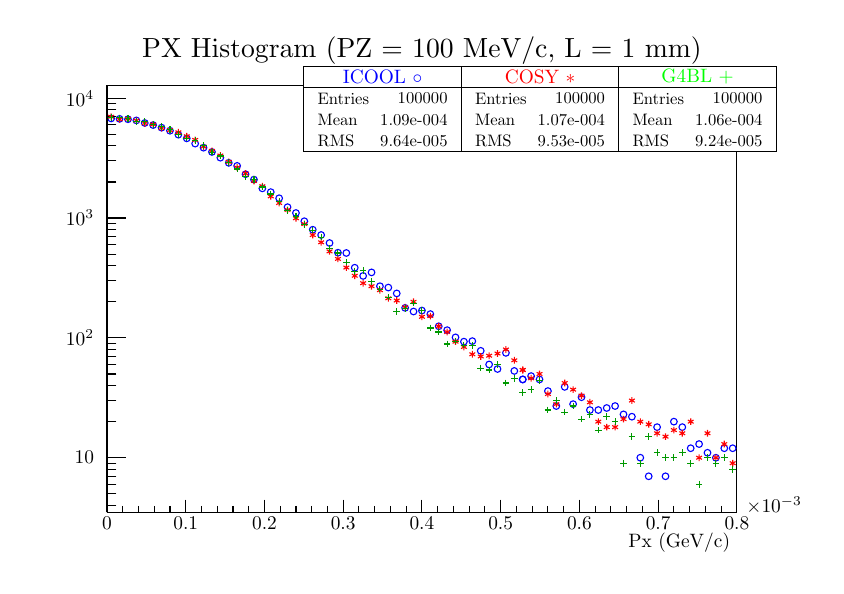
\begin{tikzpicture}
\definecolor{c}{rgb}{1,1,1};
\definecolor{blue}{rgb}{0,0,1};
\definecolor{red}{rgb}{1,0,0};
\definecolor{green}{rgb}{0,1,0};
\draw [color=c, fill=c] (0,0) rectangle (20,13.5632);
\draw [color=c, fill=c] (2,1.35632) rectangle (18,12.2069);
\definecolor{c}{rgb}{0,0,0};
\draw [c] (2,1.35632) -- (2,12.2069) -- (18,12.2069) -- (18,1.35632) -- (2,1.35632);
\definecolor{c}{rgb}{1,1,1};
\draw [color=c, fill=c] (2,1.35632) rectangle (18,12.2069);
\definecolor{c}{rgb}{0,0,0};
\draw [c] (2,1.35632) -- (2,12.2069) -- (18,12.2069) -- (18,1.35632) -- (2,1.35632);
\definecolor{c}{rgb}{0,0,1};
\foreach \P in
 {(2.10667,11.3621),(2.32,11.3517),(2.53333,11.3411),(2.74667,11.3114),(2.96,11.2463),(3.17333,11.1935),(3.38667,11.1277),(3.6,11.0501),(3.81333,10.9496),(4.02667,10.8555),(4.24,10.7227),(4.45333,10.6188),(4.66667,10.5109),(4.88,10.3651),(5.09333,10.
234),(5.30667,10.1568),(5.52,9.94466),(5.73333,9.80798),(5.94667,9.58566),(6.16,9.4904),(6.37333,9.3346),(6.58667,9.1085),(6.8,8.96002),(7.01333,8.75124),(7.22667,8.53501),(7.44,8.40105),(7.65333,8.19758),(7.86667,7.95187),(8.08,7.94413),(8.29333,7.5
6987),(8.50667,7.36208),(8.72,7.45141),(8.93333,7.10083),(9.14667,7.06611),(9.36,6.9173),(9.57333,6.55008),(9.78667,6.45781),(10,6.48149),(10.2133,6.39252),(10.4267,6.08283),(10.64,5.98405),(10.8533,5.80101),(11.0667,5.69192),(11.28,5.70606),(11.4933
,5.45941),(11.7067,5.1126),(11.92,4.99758),(12.1333,5.40757),(12.3467,4.94861),(12.56,4.73231)}{\draw[mark options={color=c,fill=c},mark size=2.402402pt,mark=o] plot coordinates {\P};}
\foreach \P in
 {(12.56,4.73231),(12.7733,4.81762),(12.9867,4.73231),(13.2,4.43734),(13.4133,4.05705),(13.6267,4.54315),(13.84,4.10513),(14.0533,4.28164),(14.2667,3.95532),(14.48,3.95532),(14.6933,4.00716),(14.9067,4.05705),(15.12,3.8451),(15.3333,3.78634),(15.5467
,2.74408),(15.76,2.27259),(15.9733,3.52107),(16.1867,2.27259),(16.4,3.66035),(16.6133,3.52107),(16.8267,2.98509),(17.04,3.0909),(17.2533,2.87007),(17.4667,2.74408),(17.68,2.98509),(17.8933,2.98509)}{\draw[mark options={color=c,fill=c},mark
 size=2.402402pt,mark=o] plot coordinates {\P};}
\definecolor{c}{rgb}{1,1,1};
\draw [color=c, fill=c] (7,10.5115) rectangle (11,12.6816);
\definecolor{c}{rgb}{0,0,0};
\draw [c] (7,10.5115) -- (11,10.5115);
\draw [c] (11,10.5115) -- (11,12.6816);
\draw [c] (11,12.6816) -- (7,12.6816);
\draw [c] (7,12.6816) -- (7,10.5115);
%\draw (9,12.4103) node[scale=1.10854, rotate=0]{ICOOL};
\draw [color=blue] (9,12.4103) node[scale=0.7, rotate=0]{ICOOL $\circ$};
\draw [c] (7,12.1391) -- (11,12.1391);
\draw [anchor= west] (7.2,11.8678) node[scale=0.6,rotate=0]{Entries };
\draw [anchor= east] (10.8,11.8678) node[scale=0.6,rotate=0]{ 100000};
\draw [anchor= west] (7.2,11.3253) node[scale=0.6,rotate=0]{Mean  };
\draw [anchor= east] (10.8,11.3253) node[scale=0.6,rotate=0]{ 1.09e-004};
\draw [anchor= west] (7.2,10.7828) node[scale=0.6,rotate=0]{RMS   };
\draw [anchor= east] (10.8,10.7828) node[scale=0.6,rotate=0]{ 9.64e-005};
\draw [c] (2,1.35632) -- (18,1.35632);
\draw [anchor= east] (18,0.596782) node[scale=0.7, rotate=0]{Px (GeV/c)};
\draw [c] (2,1.68184) -- (2,1.35632);
\draw [c] (2.4,1.51908) -- (2.4,1.35632);
\draw [c] (2.8,1.51908) -- (2.8,1.35632);
\draw [c] (3.2,1.51908) -- (3.2,1.35632);
\draw [c] (3.6,1.51908) -- (3.6,1.35632);
\draw [c] (4,1.68184) -- (4,1.35632);
\draw [c] (4.4,1.51908) -- (4.4,1.35632);
\draw [c] (4.8,1.51908) -- (4.8,1.35632);
\draw [c] (5.2,1.51908) -- (5.2,1.35632);
\draw [c] (5.6,1.51908) -- (5.6,1.35632);
\draw [c] (6,1.68184) -- (6,1.35632);
\draw [c] (6.4,1.51908) -- (6.4,1.35632);
\draw [c] (6.8,1.51908) -- (6.8,1.35632);
\draw [c] (7.2,1.51908) -- (7.2,1.35632);
\draw [c] (7.6,1.51908) -- (7.6,1.35632);
\draw [c] (8,1.68184) -- (8,1.35632);
\draw [c] (8.4,1.51908) -- (8.4,1.35632);
\draw [c] (8.8,1.51908) -- (8.8,1.35632);
\draw [c] (9.2,1.51908) -- (9.2,1.35632);
\draw [c] (9.6,1.51908) -- (9.6,1.35632);
\draw [c] (10,1.68184) -- (10,1.35632);
\draw [c] (10.4,1.51908) -- (10.4,1.35632);
\draw [c] (10.8,1.51908) -- (10.8,1.35632);
\draw [c] (11.2,1.51908) -- (11.2,1.35632);
\draw [c] (11.6,1.51908) -- (11.6,1.35632);
\draw [c] (12,1.68184) -- (12,1.35632);
\draw [c] (12.4,1.51908) -- (12.4,1.35632);
\draw [c] (12.8,1.51908) -- (12.8,1.35632);
\draw [c] (13.2,1.51908) -- (13.2,1.35632);
\draw [c] (13.6,1.51908) -- (13.6,1.35632);
\draw [c] (14,1.68184) -- (14,1.35632);
\draw [c] (14.4,1.51908) -- (14.4,1.35632);
\draw [c] (14.8,1.51908) -- (14.8,1.35632);
\draw [c] (15.2,1.51908) -- (15.2,1.35632);
\draw [c] (15.6,1.51908) -- (15.6,1.35632);
\draw [c] (16,1.68184) -- (16,1.35632);
\draw [c] (16.4,1.51908) -- (16.4,1.35632);
\draw [c] (16.8,1.51908) -- (16.8,1.35632);
\draw [c] (17.2,1.51908) -- (17.2,1.35632);
\draw [c] (17.6,1.51908) -- (17.6,1.35632);
\draw [c] (18,1.68184) -- (18,1.35632);
\draw [anchor=base] (2,0.908736) node[scale=0.7, rotate=0]{0};
\draw [anchor=base] (4,0.908736) node[scale=0.7, rotate=0]{0.1};
\draw [anchor=base] (6,0.908736) node[scale=0.7, rotate=0]{0.2};
\draw [anchor=base] (8,0.908736) node[scale=0.7, rotate=0]{0.3};
\draw [anchor=base] (10,0.908736) node[scale=0.7, rotate=0]{0.4};
\draw [anchor=base] (12,0.908736) node[scale=0.7, rotate=0]{0.5};
\draw [anchor=base] (14,0.908736) node[scale=0.7, rotate=0]{0.6};
\draw [anchor=base] (16,0.908736) node[scale=0.7, rotate=0]{0.7};
\draw [anchor=base] (18,0.908736) node[scale=0.7, rotate=0]{0.8};
\draw [anchor=base west] (18.07,1.35632) node[scale=0.7, rotate=0]{$\times10^{-3}$};
\draw [c] (2,1.35632) -- (2,12.2069);
\draw [c] (2.24,1.53283) -- (2,1.53283);
\draw [c] (2.24,1.82781) -- (2,1.82781);
\draw [c] (2.24,2.06882) -- (2,2.06882);
\draw [c] (2.24,2.27259) -- (2,2.27259);
\draw [c] (2.24,2.4491) -- (2,2.4491);
\draw [c] (2.24,2.6048) -- (2,2.6048);
\draw [c] (2.48,2.74407) -- (2,2.74407);
\draw [anchor= east] (1.844,2.74407) node[scale=0.7, rotate=0]{10};
\draw [c] (2.24,3.66034) -- (2,3.66034);
\draw [c] (2.24,4.19633) -- (2,4.19633);
\draw [c] (2.24,4.57661) -- (2,4.57661);
\draw [c] (2.24,4.87158) -- (2,4.87158);
\draw [c] (2.24,5.11259) -- (2,5.11259);
\draw [c] (2.24,5.31637) -- (2,5.31637);
\draw [c] (2.24,5.49288) -- (2,5.49288);
\draw [c] (2.24,5.64858) -- (2,5.64858);
\draw [c] (2.48,5.78785) -- (2,5.78785);
\draw [anchor= east] (1.844,5.78785) node[scale=0.7, rotate=0]{$10^{2}$};
\draw [c] (2.24,6.70412) -- (2,6.70412);
\draw [c] (2.24,7.2401) -- (2,7.2401);
\draw [c] (2.24,7.62039) -- (2,7.62039);
\draw [c] (2.24,7.91536) -- (2,7.91536);
\draw [c] (2.24,8.15637) -- (2,8.15637);
\draw [c] (2.24,8.36014) -- (2,8.36014);
\draw [c] (2.24,8.53666) -- (2,8.53666);
\draw [c] (2.24,8.69236) -- (2,8.69236);
\draw [c] (2.48,8.83163) -- (2,8.83163);
\draw [anchor= east] (1.844,8.83163) node[scale=0.7, rotate=0]{$10^{3}$};
\draw [c] (2.24,9.7479) -- (2,9.7479);
\draw [c] (2.24,10.2839) -- (2,10.2839);
\draw [c] (2.24,10.6642) -- (2,10.6642);
\draw [c] (2.24,10.9591) -- (2,10.9591);
\draw [c] (2.24,11.2002) -- (2,11.2002);
\draw [c] (2.24,11.4039) -- (2,11.4039);
\draw [c] (2.24,11.5804) -- (2,11.5804);
\draw [c] (2.24,11.7361) -- (2,11.7361);
\draw [c] (2.48,11.8754) -- (2,11.8754);
\draw [anchor= east] (1.844,11.8754) node[scale=0.7, rotate=0]{$10^{4}$};
\definecolor{c}{rgb}{1,1,1};
\draw [color=c, fill=c] (7,10.5115) rectangle (11,12.6816);
\definecolor{c}{rgb}{0,0,0};
\draw [c] (7,10.5115) -- (11,10.5115);
\draw [c] (11,10.5115) -- (11,12.6816);
\draw [c] (11,12.6816) -- (7,12.6816);
\draw [c] (7,12.6816) -- (7,10.5115);
%\draw [color=blue](9,12.4103) node[scale=1.10854, rotate=0]{ICOOL};
\draw [color=blue](9,12.4103) node[scale=0.7, rotate=0]{ICOOL $\circ$};
\draw [c] (7,12.1391) -- (11,12.1391);
\draw [anchor= west] (7.2,11.8678) node[scale=0.6,rotate=0]{Entries };
\draw [anchor= east] (10.8,11.8678) node[scale=0.6,rotate=0]{ 100000};
\draw [anchor= west] (7.2,11.3253) node[scale=0.6,rotate=0]{Mean  };
\draw [anchor= east] (10.8,11.3253) node[scale=0.6,rotate=0]{ 1.09e-004};
\draw [anchor= west] (7.2,10.7828) node[scale=0.6,rotate=0]{RMS   };
\draw [anchor= east] (10.8,10.7828) node[scale=0.6,rotate=0]{ 9.64e-005};
\draw (10,13.0816) node[scale=1, rotate=0]{PX Histogram (PZ = 100 MeV/c, L = 1 mm)};
\definecolor{c}{rgb}{1,0,0};
\foreach \P in
 {(2.10667,11.4041),(2.32,11.3393),(2.53333,11.3525),(2.74667,11.3074),(2.96,11.2409),(3.17333,11.21),(3.38667,11.1153),(3.6,11.0648),(3.81333,11.0095),(4.02667,10.9099),(4.24,10.8166),(4.45333,10.6455),(4.66667,10.5359),(4.88,10.421),(5.09333,10.258
1),(5.30667,10.1159),(5.52,9.9622),(5.73333,9.77343),(5.94667,9.64055),(6.16,9.38251),(6.37333,9.21456),(6.58667,9.03804),(6.8,8.82633),(7.01333,8.67907),(7.22667,8.39922),(7.44,8.21456),(7.65333,7.98488),(7.86667,7.7936),(8.08,7.5733),(8.29333,7.366
1),(8.50667,7.17693),(8.72,7.10083),(8.93333,6.99909),(9.14667,6.79356),(9.36,6.73676),(9.57333,6.56485),(9.78667,6.70412),(10,6.32384),(10.2133,6.34135),(10.4267,6.08283),(10.64,5.93766),(10.8533,5.69192),(11.0667,5.55738),(11.28,5.37184),(11.4933,5
.31637),(11.7067,5.33512),(11.92,5.38982),(12.1333,5.49288),(12.3467,5.2184),(12.56,4.97332)}{\draw[mark options={color=c,fill=c},mark size=2.402402pt,mark=asterisk] plot coordinates {\P};}
\foreach \P in
 {(12.56,4.97332),(12.7733,4.76136),(12.9867,4.87159),(13.2,4.36178),(13.4133,4.10513),(13.6267,4.64111),(13.84,4.47356),(14.0533,4.32232),(14.2667,4.15151),(14.48,3.66035),(14.6933,3.52107),(14.9067,3.52107),(15.12,3.72484),(15.3333,4.19633),(15.546
7,3.66035),(15.76,3.59254),(15.9733,3.36537),(16.1867,3.28006),(16.4,3.44551),(16.6133,3.36537),(16.8267,3.66035),(17.04,2.74408),(17.2533,3.36537),(17.4667,2.74408),(17.68,3.0909),(17.8933,2.6048)}{\draw[mark options={color=c,fill=c},mark
 size=2.402402pt,mark=asterisk] plot coordinates {\P};}
\definecolor{c}{rgb}{1,1,1};
\draw [color=c, fill=c] (11,10.5115) rectangle (15,12.6816);
\definecolor{c}{rgb}{0,0,0};
\draw [c] (11,10.5115) -- (15,10.5115);
\draw [c] (15,10.5115) -- (15,12.6816);
\draw [c] (15,12.6816) -- (11,12.6816);
\draw [c] (11,12.6816) -- (11,10.5115);
\draw [color=red](13,12.4103) node[scale=0.7, rotate=0]{COSY $*$};
\draw [c] (11,12.1391) -- (15,12.1391);
\draw [anchor= west] (11.2,11.8678) node[scale=0.6,rotate=0]{Entries };
\draw [anchor= east] (14.8,11.8678) node[scale=0.6,rotate=0]{ 100000};
\draw [anchor= west] (11.2,11.3253) node[scale=0.6,rotate=0]{Mean  };
\draw [anchor= east] (14.8,11.3253) node[scale=0.6,rotate=0]{ 1.07e-004};
\draw [anchor= west] (11.2,10.7828) node[scale=0.6,rotate=0]{RMS   };
\draw [anchor= east] (14.8,10.7828) node[scale=0.6,rotate=0]{ 9.53e-005};
\definecolor{c}{rgb}{1,1,1};
\draw [color=c, fill=c] (11,10.5115) rectangle (15,12.6816);
\definecolor{c}{rgb}{0,0,0};
\draw [c] (11,10.5115) -- (15,10.5115);
\draw [c] (15,10.5115) -- (15,12.6816);
\draw [c] (15,12.6816) -- (11,12.6816);
\draw [c] (11,12.6816) -- (11,10.5115);
\draw [color=red](13,12.4103) node[scale=0.7, rotate=0]{COSY $*$};
\draw [c] (11,12.1391) -- (15,12.1391);
\draw [anchor= west] (11.2,11.8678) node[scale=0.6,rotate=0]{Entries };
\draw [anchor= east] (14.8,11.8678) node[scale=0.6,rotate=0]{ 100000};
\draw [anchor= west] (11.2,11.3253) node[scale=0.6,rotate=0]{Mean  };
\draw [anchor= east] (14.8,11.3253) node[scale=0.6,rotate=0]{ 1.07e-004};
\draw [anchor= west] (11.2,10.7828) node[scale=0.6,rotate=0]{RMS   };
\draw [anchor= east] (14.8,10.7828) node[scale=0.6,rotate=0]{ 9.53e-005};
\definecolor{c}{rgb}{0,0.6,0};
\foreach \P in
 {(2.10667,11.3914),(2.32,11.3761),(2.53333,11.3652),(2.74667,11.2919),(2.96,11.2778),(3.17333,11.2092),(3.38667,11.154),(3.6,11.0767),(3.81333,10.9578),(4.02667,10.8635),(4.24,10.7991),(4.45333,10.6714),(4.66667,10.5057),(4.88,10.4087),(5.09333,10.2
477),(5.30667,10.0768),(5.52,9.88704),(5.73333,9.81302),(5.94667,9.62105),(6.16,9.44298),(6.37333,9.25067),(6.58667,9.02555),(6.8,8.88221),(7.01333,8.66864),(7.22667,8.52671),(7.44,8.34686),(7.65333,8.06517),(7.86667,7.94413),(8.08,7.71291),(8.29333,
7.48112),(8.50667,7.49209),(8.72,7.2134),(8.93333,7.02527),(9.14667,6.82409),(9.36,6.46575),(9.57333,6.53514),(9.78667,6.67065),(10,6.48929),(10.2133,6.03983),(10.4267,5.93766),(10.64,5.63381),(10.8533,5.70606),(11.0667,5.60376),(11.28,5.58848),(11.4
933,5.02139),(11.7067,4.97332),(11.92,5.1126),(12.1333,4.64111),(12.3467,4.76136),(12.56,4.4001)}{\draw[mark options={color=c,fill=c},mark size=2.402402pt,mark=+] plot coordinates {\P};}
\foreach \P in
 {(12.56,4.4001),(12.7733,4.47356),(12.9867,4.7026),(13.2,3.95532),(13.4133,4.19633),(13.6267,3.90136),(13.84,4.05705),(14.0533,3.72484),(14.2667,3.8451),(14.48,3.44551),(14.6933,3.78634),(14.9067,3.66035),(15.12,2.6048),(15.3333,3.28006),(15.5467,2.
6048),(15.76,3.28006),(15.9733,2.87007),(16.1867,2.74408),(16.4,2.74408),(16.6133,2.87007),(16.8267,2.6048),(17.04,2.06882),(17.2533,2.74408),(17.4667,2.6048),(17.68,2.74408),(17.8933,2.4491)}{\draw[mark options={color=c,fill=c},mark
 size=2.402402pt,mark=+] plot coordinates {\P};}
\definecolor{c}{rgb}{1,1,1};
\draw [color=c, fill=c] (15,10.5115) rectangle (19,12.6816);
\definecolor{c}{rgb}{0,0,0};
\draw [c] (15,10.5115) -- (19,10.5115);
\draw [c] (19,10.5115) -- (19,12.6816);
\draw [c] (19,12.6816) -- (15,12.6816);
\draw [c] (15,12.6816) -- (15,10.5115);
\draw [color=green](17,12.4103) node[scale=0.7, rotate=0]{G4BL $+$};
\draw [c] (15,12.1391) -- (19,12.1391);
\draw [anchor= west] (15.2,11.8678) node[scale=0.6,rotate=0]{Entries };
\draw [anchor= east] (18.8,11.8678) node[scale=0.6,rotate=0]{ 100000};
\draw [anchor= west] (15.2,11.3253) node[scale=0.6,rotate=0]{Mean  };
\draw [anchor= east] (18.8,11.3253) node[scale=0.6,rotate=0]{ 1.06e-004};
\draw [anchor= west] (15.2,10.7828) node[scale=0.6,rotate=0]{RMS   };
\draw [anchor= east] (18.8,10.7828) node[scale=0.6,rotate=0]{ 9.24e-005};
\definecolor{c}{rgb}{1,1,1};
\draw [color=c, fill=c] (15,10.5115) rectangle (19,12.6816);
\definecolor{c}{rgb}{0,0,0};
\draw [c] (15,10.5115) -- (19,10.5115);
\draw [c] (19,10.5115) -- (19,12.6816);
\draw [c] (19,12.6816) -- (15,12.6816);
\draw [c] (15,12.6816) -- (15,10.5115);
\draw [color=green](17,12.4103) node[scale=0.7, rotate=0]{G4BL $+$};
\draw [c] (15,12.1391) -- (19,12.1391);
\draw [anchor= west] (15.2,11.8678) node[scale=0.6,rotate=0]{Entries };
\draw [anchor= east] (18.8,11.8678) node[scale=0.6,rotate=0]{ 100000};
\draw [anchor= west] (15.2,11.3253) node[scale=0.6,rotate=0]{Mean  };
\draw [anchor= east] (18.8,11.3253) node[scale=0.6,rotate=0]{ 1.06e-004};
\draw [anchor= west] (15.2,10.7828) node[scale=0.6,rotate=0]{RMS   };
\draw [anchor= east] (18.8,10.7828) node[scale=0.6,rotate=0]{ 9.24e-005};
\end{tikzpicture}
}\\
\frame{\pgfdeclareplotmark{cross} {
\pgfpathmoveto{\pgfpoint{-0.3\pgfplotmarksize}{\pgfplotmarksize}}
\pgfpathlineto{\pgfpoint{+0.3\pgfplotmarksize}{\pgfplotmarksize}}
\pgfpathlineto{\pgfpoint{+0.3\pgfplotmarksize}{0.3\pgfplotmarksize}}
\pgfpathlineto{\pgfpoint{+1\pgfplotmarksize}{0.3\pgfplotmarksize}}
\pgfpathlineto{\pgfpoint{+1\pgfplotmarksize}{-0.3\pgfplotmarksize}}
\pgfpathlineto{\pgfpoint{+0.3\pgfplotmarksize}{-0.3\pgfplotmarksize}}
\pgfpathlineto{\pgfpoint{+0.3\pgfplotmarksize}{-1.\pgfplotmarksize}}
\pgfpathlineto{\pgfpoint{-0.3\pgfplotmarksize}{-1.\pgfplotmarksize}}
\pgfpathlineto{\pgfpoint{-0.3\pgfplotmarksize}{-0.3\pgfplotmarksize}}
\pgfpathlineto{\pgfpoint{-1.\pgfplotmarksize}{-0.3\pgfplotmarksize}}
\pgfpathlineto{\pgfpoint{-1.\pgfplotmarksize}{0.3\pgfplotmarksize}}
\pgfpathlineto{\pgfpoint{-0.3\pgfplotmarksize}{0.3\pgfplotmarksize}}
\pgfpathclose
\pgfusepathqstroke
}
\pgfdeclareplotmark{cross*} {
\pgfpathmoveto{\pgfpoint{-0.3\pgfplotmarksize}{\pgfplotmarksize}}
\pgfpathlineto{\pgfpoint{+0.3\pgfplotmarksize}{\pgfplotmarksize}}
\pgfpathlineto{\pgfpoint{+0.3\pgfplotmarksize}{0.3\pgfplotmarksize}}
\pgfpathlineto{\pgfpoint{+1\pgfplotmarksize}{0.3\pgfplotmarksize}}
\pgfpathlineto{\pgfpoint{+1\pgfplotmarksize}{-0.3\pgfplotmarksize}}
\pgfpathlineto{\pgfpoint{+0.3\pgfplotmarksize}{-0.3\pgfplotmarksize}}
\pgfpathlineto{\pgfpoint{+0.3\pgfplotmarksize}{-1.\pgfplotmarksize}}
\pgfpathlineto{\pgfpoint{-0.3\pgfplotmarksize}{-1.\pgfplotmarksize}}
\pgfpathlineto{\pgfpoint{-0.3\pgfplotmarksize}{-0.3\pgfplotmarksize}}
\pgfpathlineto{\pgfpoint{-1.\pgfplotmarksize}{-0.3\pgfplotmarksize}}
\pgfpathlineto{\pgfpoint{-1.\pgfplotmarksize}{0.3\pgfplotmarksize}}
\pgfpathlineto{\pgfpoint{-0.3\pgfplotmarksize}{0.3\pgfplotmarksize}}
\pgfpathclose
\pgfusepathqfillstroke
}
\pgfdeclareplotmark{newstar} {
\pgfpathmoveto{\pgfqpoint{0pt}{\pgfplotmarksize}}
\pgfpathlineto{\pgfqpointpolar{44}{0.5\pgfplotmarksize}}
\pgfpathlineto{\pgfqpointpolar{18}{\pgfplotmarksize}}
\pgfpathlineto{\pgfqpointpolar{-20}{0.5\pgfplotmarksize}}
\pgfpathlineto{\pgfqpointpolar{-54}{\pgfplotmarksize}}
\pgfpathlineto{\pgfqpointpolar{-90}{0.5\pgfplotmarksize}}
\pgfpathlineto{\pgfqpointpolar{234}{\pgfplotmarksize}}
\pgfpathlineto{\pgfqpointpolar{198}{0.5\pgfplotmarksize}}
\pgfpathlineto{\pgfqpointpolar{162}{\pgfplotmarksize}}
\pgfpathlineto{\pgfqpointpolar{134}{0.5\pgfplotmarksize}}
\pgfpathclose
\pgfusepathqstroke
}
\pgfdeclareplotmark{newstar*} {
\pgfpathmoveto{\pgfqpoint{0pt}{\pgfplotmarksize}}
\pgfpathlineto{\pgfqpointpolar{44}{0.5\pgfplotmarksize}}
\pgfpathlineto{\pgfqpointpolar{18}{\pgfplotmarksize}}
\pgfpathlineto{\pgfqpointpolar{-20}{0.5\pgfplotmarksize}}
\pgfpathlineto{\pgfqpointpolar{-54}{\pgfplotmarksize}}
\pgfpathlineto{\pgfqpointpolar{-90}{0.5\pgfplotmarksize}}
\pgfpathlineto{\pgfqpointpolar{234}{\pgfplotmarksize}}
\pgfpathlineto{\pgfqpointpolar{198}{0.5\pgfplotmarksize}}
\pgfpathlineto{\pgfqpointpolar{162}{\pgfplotmarksize}}
\pgfpathlineto{\pgfqpointpolar{134}{0.5\pgfplotmarksize}}
\pgfpathclose
\pgfusepathqfillstroke
}
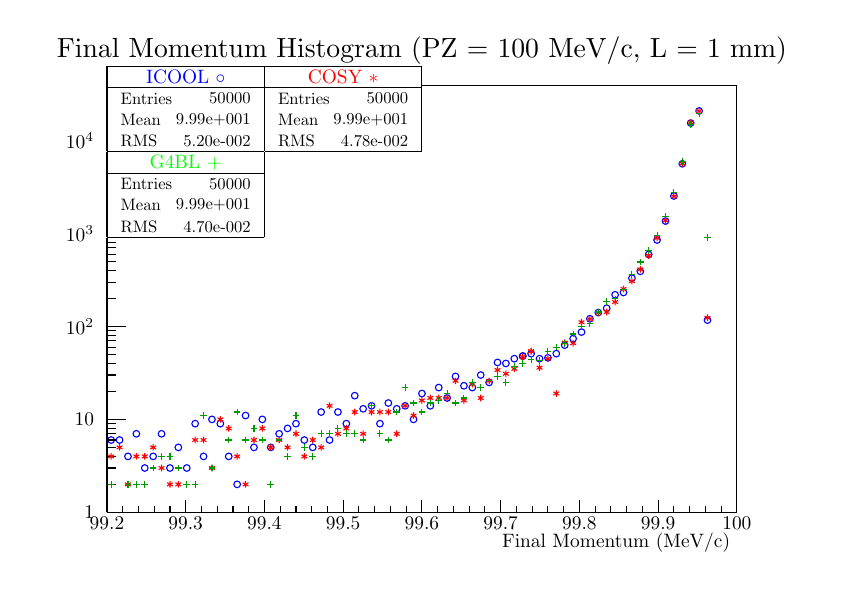
\begin{tikzpicture}
\definecolor{c}{rgb}{1,1,1};
\draw [color=c, fill=c] (0,0) rectangle (20,13.5632);
\draw [color=c, fill=c] (2,1.35632) rectangle (18,12.2069);
\definecolor{c}{rgb}{0,0,0};
\draw [c] (2,1.35632) -- (2,12.2069) -- (18,12.2069) -- (18,1.35632) -- (2,1.35632);
\definecolor{c}{rgb}{1,1,1};
\draw [color=c, fill=c] (2,1.35632) rectangle (18,12.2069);
\definecolor{c}{rgb}{0,0,0};
\draw [c] (2,1.35632) -- (2,12.2069) -- (18,12.2069) -- (18,1.35632) -- (2,1.35632);
\definecolor{c}{rgb}{0,0,1};
\foreach \P in
 {(2.10667,3.19358),(2.32,3.19358),(2.53333,2.77782),(2.74667,3.35164),(2.96,2.48283),(3.17333,2.77782),(3.38667,3.35164),(3.6,2.48283),(3.81333,3.00663),(4.02667,2.48283),(4.24,3.60934),(4.45333,2.77782),(4.66667,3.71737),(4.88,3.60934),(5.09333,2.7
7782),(5.30667,2.06707),(5.52,3.8151),(5.73333,3.00663),(5.94667,3.71737),(6.16,3.00663),(6.37333,3.35164),(6.58667,3.48856),(6.8,3.60934),(7.01333,3.19358),(7.22667,3.00663),(7.44,3.90432),(7.65333,3.19358),(7.86667,3.90432),(8.08,3.60934),(8.29333,
4.32008),(8.50667,3.9864),(8.72,4.06239),(8.93333,3.60934),(9.14667,4.13313),(9.36,3.9864),(9.57333,4.06239),(9.78667,3.71737),(10,4.37552),(10.2133,4.06239),(10.4267,4.52585),(10.64,4.26147),(10.8533,4.80912),(11.0667,4.57143),(11.28,4.52585),(11.49
33,4.84388),(11.7067,4.65693),(11.92,5.16419),(12.1333,5.13887),(12.3467,5.25964),(12.56,5.32582)}{\draw[mark options={color=c,fill=c},mark size=2.402402pt,mark=o] plot coordinates {\P};}
\foreach \P in
 {(12.56,5.32582),(12.7733,5.38798),(12.9867,5.25964),(13.2,5.28218),(13.4133,5.38798),(13.6267,5.60466),(13.84,5.76967),(14.0533,5.93563),(14.2667,6.27388),(14.48,6.43074),(14.6933,6.54095),(14.9067,6.88223),(15.12,6.94136),(15.3333,7.30266),(15.546
7,7.4792),(15.76,7.9071),(15.9733,8.27404),(16.1867,8.75552),(16.4,9.39207),(16.6133,10.2104),(16.8267,11.2444),(17.04,11.5516),(17.2533,6.23941)}{\draw[mark options={color=c,fill=c},mark size=2.402402pt,mark=o] plot coordinates {\P};}
\definecolor{c}{rgb}{1,1,1};
\draw [color=c, fill=c] (2,10.5115) rectangle (6,12.6816);
\definecolor{c}{rgb}{0,0,0};
\draw [c] (2,10.5115) -- (6,10.5115);
\draw [c] (6,10.5115) -- (6,12.6816);
\draw [c] (6,12.6816) -- (2,12.6816);
\draw [c] (2,12.6816) -- (2,10.5115);
\draw[color=blue](4,12.4103) node[scale=0.7, rotate=0]{ICOOL $\circ$};
\draw [c] (2,12.1391) -- (6,12.1391);
\draw [anchor= west] (2.2,11.8678) node[scale=0.6, rotate=0]{Entries };
\draw [anchor= east] (5.8,11.8678) node[scale=0.6, rotate=0]{ 50000};
\draw [anchor= west] (2.2,11.3253) node[scale=0.6, rotate=0]{Mean  };
\draw [anchor= east] (5.8,11.3253) node[scale=0.6, rotate=0]{ 9.99e+001};
\draw [anchor= west] (2.2,10.7828) node[scale=0.6, rotate=0]{RMS   };
\draw [anchor= east] (5.8,10.7828) node[scale=0.6, rotate=0]{ 5.20e-002};
\draw [c] (2,1.35632) -- (18,1.35632);
\draw [anchor= east] (18,0.596782) node[scale=0.7, rotate=0]{Final Momentum (MeV/c)};
\draw [c] (2,1.68184) -- (2,1.35632);
\draw [c] (2.4,1.51908) -- (2.4,1.35632);
\draw [c] (2.8,1.51908) -- (2.8,1.35632);
\draw [c] (3.2,1.51908) -- (3.2,1.35632);
\draw [c] (3.6,1.51908) -- (3.6,1.35632);
\draw [c] (4,1.68184) -- (4,1.35632);
\draw [c] (4.4,1.51908) -- (4.4,1.35632);
\draw [c] (4.8,1.51908) -- (4.8,1.35632);
\draw [c] (5.2,1.51908) -- (5.2,1.35632);
\draw [c] (5.6,1.51908) -- (5.6,1.35632);
\draw [c] (6,1.68184) -- (6,1.35632);
\draw [c] (6.4,1.51908) -- (6.4,1.35632);
\draw [c] (6.8,1.51908) -- (6.8,1.35632);
\draw [c] (7.2,1.51908) -- (7.2,1.35632);
\draw [c] (7.6,1.51908) -- (7.6,1.35632);
\draw [c] (8,1.68184) -- (8,1.35632);
\draw [c] (8.4,1.51908) -- (8.4,1.35632);
\draw [c] (8.8,1.51908) -- (8.8,1.35632);
\draw [c] (9.2,1.51908) -- (9.2,1.35632);
\draw [c] (9.6,1.51908) -- (9.6,1.35632);
\draw [c] (10,1.68184) -- (10,1.35632);
\draw [c] (10.4,1.51908) -- (10.4,1.35632);
\draw [c] (10.8,1.51908) -- (10.8,1.35632);
\draw [c] (11.2,1.51908) -- (11.2,1.35632);
\draw [c] (11.6,1.51908) -- (11.6,1.35632);
\draw [c] (12,1.68184) -- (12,1.35632);
\draw [c] (12.4,1.51908) -- (12.4,1.35632);
\draw [c] (12.8,1.51908) -- (12.8,1.35632);
\draw [c] (13.2,1.51908) -- (13.2,1.35632);
\draw [c] (13.6,1.51908) -- (13.6,1.35632);
\draw [c] (14,1.68184) -- (14,1.35632);
\draw [c] (14.4,1.51908) -- (14.4,1.35632);
\draw [c] (14.8,1.51908) -- (14.8,1.35632);
\draw [c] (15.2,1.51908) -- (15.2,1.35632);
\draw [c] (15.6,1.51908) -- (15.6,1.35632);
\draw [c] (16,1.68184) -- (16,1.35632);
\draw [c] (16.4,1.51908) -- (16.4,1.35632);
\draw [c] (16.8,1.51908) -- (16.8,1.35632);
\draw [c] (17.2,1.51908) -- (17.2,1.35632);
\draw [c] (17.6,1.51908) -- (17.6,1.35632);
\draw [c] (18,1.68184) -- (18,1.35632);
\draw [c] (18,1.68184) -- (18,1.35632);
\draw [anchor=base] (2,0.908736) node[scale=0.7, rotate=0]{99.2};
\draw [anchor=base] (4,0.908736) node[scale=0.7, rotate=0]{99.3};
\draw [anchor=base] (6,0.908736) node[scale=0.7, rotate=0]{99.4};
\draw [anchor=base] (8,0.908736) node[scale=0.7, rotate=0]{99.5};
\draw [anchor=base] (10,0.908736) node[scale=0.7, rotate=0]{99.6};
\draw [anchor=base] (12,0.908736) node[scale=0.7, rotate=0]{99.7};
\draw [anchor=base] (14,0.908736) node[scale=0.7, rotate=0]{99.8};
\draw [anchor=base] (16,0.908736) node[scale=0.7, rotate=0]{99.9};
\draw [anchor=base] (18,0.908736) node[scale=0.7, rotate=0]{100};
\draw [c] (2,1.35632) -- (2,12.2069);
\draw [c] (2.48,1.35632) -- (2,1.35632);
\draw [anchor= east] (1.844,1.35632) node[scale=0.7, rotate=0]{1};
\draw [c] (2.24,2.06707) -- (2,2.06707);
\draw [c] (2.24,2.48283) -- (2,2.48283);
\draw [c] (2.24,2.77782) -- (2,2.77782);
\draw [c] (2.24,3.00663) -- (2,3.00663);
\draw [c] (2.24,3.19358) -- (2,3.19358);
\draw [c] (2.24,3.35164) -- (2,3.35164);
\draw [c] (2.24,3.48857) -- (2,3.48857);
\draw [c] (2.24,3.60934) -- (2,3.60934);
\draw [c] (2.48,3.71737) -- (2,3.71737);
\draw [anchor= east] (1.844,3.71737) node[scale=0.7, rotate=0]{10};
\draw [c] (2.24,4.42812) -- (2,4.42812);
\draw [c] (2.24,4.84388) -- (2,4.84388);
\draw [c] (2.24,5.13887) -- (2,5.13887);
\draw [c] (2.24,5.36768) -- (2,5.36768);
\draw [c] (2.24,5.55463) -- (2,5.55463);
\draw [c] (2.24,5.71269) -- (2,5.71269);
\draw [c] (2.24,5.84962) -- (2,5.84962);
\draw [c] (2.24,5.97039) -- (2,5.97039);
\draw [c] (2.48,6.07843) -- (2,6.07843);
\draw [anchor= east] (1.844,6.07843) node[scale=0.7, rotate=0]{$10^{2}$};
\draw [c] (2.24,6.78917) -- (2,6.78917);
\draw [c] (2.24,7.20493) -- (2,7.20493);
\draw [c] (2.24,7.49992) -- (2,7.49992);
\draw [c] (2.24,7.72873) -- (2,7.72873);
\draw [c] (2.24,7.91568) -- (2,7.91568);
\draw [c] (2.24,8.07374) -- (2,8.07374);
\draw [c] (2.24,8.21067) -- (2,8.21067);
\draw [c] (2.24,8.33144) -- (2,8.33144);
\draw [c] (2.48,8.43948) -- (2,8.43948);
\draw [anchor= east] (1.844,8.43948) node[scale=0.7, rotate=0]{$10^{3}$};
\draw [c] (2.24,9.15022) -- (2,9.15022);
\draw [c] (2.24,9.56598) -- (2,9.56598);
\draw [c] (2.24,9.86097) -- (2,9.86097);
\draw [c] (2.24,10.0898) -- (2,10.0898);
\draw [c] (2.24,10.2767) -- (2,10.2767);
\draw [c] (2.24,10.4348) -- (2,10.4348);
\draw [c] (2.24,10.5717) -- (2,10.5717);
\draw [c] (2.24,10.6925) -- (2,10.6925);
\draw [c] (2.48,10.8005) -- (2,10.8005);
\draw [anchor= east] (1.844,10.8005) node[scale=0.7, rotate=0]{$10^{4}$};
\draw [c] (2.24,11.5113) -- (2,11.5113);
\draw [c] (2.24,11.927) -- (2,11.927);
\definecolor{c}{rgb}{1,1,1};
\draw [color=c, fill=c] (2,10.5115) rectangle (6,12.6816);
\definecolor{c}{rgb}{0,0,0};
\draw [c] (2,10.5115) -- (6,10.5115);
\draw [c] (6,10.5115) -- (6,12.6816);
\draw [c] (6,12.6816) -- (2,12.6816);
\draw [c] (2,12.6816) -- (2,10.5115);
\draw[color=blue](4,12.4103) node[scale=0.7, rotate=0]{ICOOL $\circ$};
\draw [c] (2,12.1391) -- (6,12.1391);
\draw [anchor= west] (2.2,11.8678) node[scale=0.6, rotate=0]{Entries };
\draw [anchor= east] (5.8,11.8678) node[scale=0.6, rotate=0]{ 50000};
\draw [anchor= west] (2.2,11.3253) node[scale=0.6, rotate=0]{Mean  };
\draw [anchor= east] (5.8,11.3253) node[scale=0.6, rotate=0]{ 9.99e+001};
\draw [anchor= west] (2.2,10.7828) node[scale=0.6, rotate=0]{RMS   };
\draw [anchor= east] (5.8,10.7828) node[scale=0.6, rotate=0]{ 5.20e-002};
\draw (10,13.0816) node[scale=1, rotate=0]{Final Momentum Histogram (PZ = 100 MeV/c, L = 1 mm)};
\definecolor{c}{rgb}{1,0,0};
\foreach \P in
 {(2.10667,2.77782),(2.32,3.00663),(2.53333,2.06707),(2.74667,2.77782),(2.96,2.77782),(3.17333,3.00663),(3.38667,2.48283),(3.6,2.06707),(3.81333,2.06707),(4.24,3.19358),(4.45333,3.19358),(4.66667,2.48283),(4.88,3.71737),(5.09333,3.48856),(5.30667,2.7
7782),(5.52,2.06707),(5.73333,3.19358),(5.94667,3.48856),(6.16,3.00663),(6.37333,3.19358),(6.58667,3.00663),(6.8,3.35164),(7.01333,2.77782),(7.22667,3.19358),(7.44,3.00663),(7.65333,4.06239),(7.86667,3.35164),(8.08,3.48856),(8.29333,3.90432),(8.50667
,3.35164),(8.72,3.90432),(8.93333,3.90432),(9.14667,3.90432),(9.36,3.35164),(9.57333,4.06239),(9.78667,3.8151),(10,4.19931),(10.2133,4.26147),(10.4267,4.26147),(10.64,4.26147),(10.8533,4.69715),(11.0667,4.19931),(11.28,4.61507),(11.4933,4.26147),(11.
7067,4.69715),(11.92,4.97222),(12.1333,4.8775),(12.3467,5.00195),(12.56,5.30423),(12.7733,5.44659)}{\draw[mark options={color=c,fill=c},mark size=2.402402pt,mark=asterisk] plot coordinates {\P};}
\foreach \P in
 {(12.7733,5.44659),(12.9867,5.03083),(13.2,5.25964),(13.4133,4.37552),(13.6267,5.66778),(13.84,5.65236),(14.0533,6.18543),(14.2667,6.26538),(14.48,6.42344),(14.6933,6.44518),(14.9067,6.69808),(15.12,7.03021),(15.3333,7.22858),(15.5467,7.52774),(15.7
6,7.87915),(15.9733,8.32343),(16.1867,8.76974),(16.4,9.38476),(16.6133,10.2169),(16.8267,11.2552),(17.04,11.5479),(17.2533,6.299)}{\draw[mark options={color=c,fill=c},mark size=2.402402pt,mark=asterisk] plot coordinates {\P};}
\definecolor{c}{rgb}{1,1,1};
\draw [color=c, fill=c] (6,10.5115) rectangle (10,12.6816);
\definecolor{c}{rgb}{0,0,0};
\draw [c] (6,10.5115) -- (10,10.5115);
\draw [c] (10,10.5115) -- (10,12.6816);
\draw [c] (10,12.6816) -- (6,12.6816);
\draw [c] (6,12.6816) -- (6,10.5115);
\draw [color=red](8,12.4103) node[scale=0.7, rotate=0]{COSY $*$};
\draw [c] (6,12.1391) -- (10,12.1391);
\draw [anchor= west] (6.2,11.8678) node[scale=0.6, rotate=0]{Entries };
\draw [anchor= east] (9.8,11.8678) node[scale=0.6, rotate=0]{ 50000};
\draw [anchor= west] (6.2,11.3253) node[scale=0.6, rotate=0]{Mean  };
\draw [anchor= east] (9.8,11.3253) node[scale=0.6, rotate=0]{ 9.99e+001};
\draw [anchor= west] (6.2,10.7828) node[scale=0.6, rotate=0]{RMS   };
\draw [anchor= east] (9.8,10.7828) node[scale=0.6, rotate=0]{ 4.78e-002};
\definecolor{c}{rgb}{1,1,1};
\draw [color=c, fill=c] (6,10.5115) rectangle (10,12.6816);
\definecolor{c}{rgb}{0,0,0};
\draw [c] (6,10.5115) -- (10,10.5115);
\draw [c] (10,10.5115) -- (10,12.6816);
\draw [c] (10,12.6816) -- (6,12.6816);
\draw [c] (6,12.6816) -- (6,10.5115);
\draw [color=red](8,12.4103) node[scale=0.7, rotate=0]{COSY $*$};
\draw [c] (6,12.1391) -- (10,12.1391);
\draw [anchor= west] (6.2,11.8678) node[scale=0.6, rotate=0]{Entries };
\draw [anchor= east] (9.8,11.8678) node[scale=0.6, rotate=0]{ 50000};
\draw [anchor= west] (6.2,11.3253) node[scale=0.6, rotate=0]{Mean  };
\draw [anchor= east] (9.8,11.3253) node[scale=0.6, rotate=0]{ 9.99e+001};
\draw [anchor= west] (6.2,10.7828) node[scale=0.6, rotate=0]{RMS   };
\draw [anchor= east] (9.8,10.7828) node[scale=0.6, rotate=0]{ 4.78e-002};
\definecolor{c}{rgb}{0,0.6,0};
\foreach \P in
 {(2.10667,2.06707),(2.53333,2.06707),(2.74667,2.06707),(2.96,2.06707),(3.17333,2.48283),(3.38667,2.77782),(3.6,2.77782),(3.81333,2.48283),(4.02667,2.06707),(4.24,2.06707),(4.45333,3.8151),(4.66667,2.48283),(5.09333,3.19358),(5.30667,3.90432),(5.52,3
.19358),(5.73333,3.48856),(5.94667,3.19358),(6.16,2.06707),(6.37333,3.19358),(6.58667,2.77782),(6.8,3.8151),(7.01333,3.00663),(7.22667,2.77782),(7.44,3.35164),(7.65333,3.35164),(7.86667,3.48856),(8.08,3.35164),(8.29333,3.35164),(8.50667,3.19358),(8.7
2,4.06239),(8.93333,3.35164),(9.14667,3.19358),(9.36,3.90432),(9.57333,4.52585),(9.78667,4.13313),(10,3.90432),(10.2133,4.13313),(10.4267,4.19931),(10.64,4.37552),(10.8533,4.13313),(11.0667,4.26147),(11.28,4.65693),(11.4933,4.52585),(11.7067,4.69715)
,(11.92,4.80912),(12.1333,4.65693),(12.3467,5.05893),(12.56,5.13887),(12.7733,5.2366),(12.9867,5.21302)}{\draw[mark options={color=c,fill=c},mark size=2.402402pt,mark=+] plot coordinates {\P};}
\foreach \P in
 {(12.9867,5.21302),(13.2,5.44659),(13.4133,5.55463),(13.6267,5.65236),(13.84,5.88736),(14.0533,6.07842),(14.2667,6.15734),(14.48,6.44518),(14.6933,6.71476),(14.9067,6.77887),(15.12,7.02615),(15.3333,7.40039),(15.5467,7.71427),(15.76,8.00718),(15.973
3,8.38364),(16.1867,8.87017),(16.4,9.49083),(16.6133,10.2611),(16.8267,11.2048),(17.04,11.4935),(17.2533,8.33825)}{\draw[mark options={color=c,fill=c},mark size=2.402402pt,mark=+] plot coordinates {\P};}
\definecolor{c}{rgb}{1,1,1};
\draw [color=c, fill=c] (2,8.34138) rectangle (6,10.5115);
\definecolor{c}{rgb}{0,0,0};
\draw [c] (2,8.34138) -- (6,8.34138);
\draw [c] (6,8.34138) -- (6,10.5115);
\draw [c] (6,10.5115) -- (2,10.5115);
\draw [c] (2,10.5115) -- (2,8.34138);
\draw [color=green](4,10.2402) node[scale=0.7, rotate=0]{G4BL $+$};
\draw [c] (2,9.96897) -- (6,9.96897);
\draw [anchor= west] (2.2,9.6977) node[scale=0.6, rotate=0]{Entries };
\draw [anchor= east] (5.8,9.6977) node[scale=0.6, rotate=0]{ 50000};
\draw [anchor= west] (2.2,9.15517) node[scale=0.6, rotate=0]{Mean  };
\draw [anchor= east] (5.8,9.15517) node[scale=0.6, rotate=0]{ 9.99e+001};
\draw [anchor= west] (2.2,8.61264) node[scale=0.6, rotate=0]{RMS   };
\draw [anchor= east] (5.8,8.61264) node[scale=0.6, rotate=0]{ 4.70e-002};
\definecolor{c}{rgb}{1,1,1};
\draw [color=c, fill=c] (2,8.34138) rectangle (6,10.5115);
\definecolor{c}{rgb}{0,0,0};
\draw [c] (2,8.34138) -- (6,8.34138);
\draw [c] (6,8.34138) -- (6,10.5115);
\draw [c] (6,10.5115) -- (2,10.5115);
\draw [c] (2,10.5115) -- (2,8.34138);
\draw [color=green](4,10.2402) node[scale=0.7, rotate=0]{G4BL $+$};
\draw [c] (2,9.96897) -- (6,9.96897);
\draw [anchor= west] (2.2,9.6977) node[scale=0.6, rotate=0]{Entries };
\draw [anchor= east] (5.8,9.6977) node[scale=0.6, rotate=0]{ 50000};
\draw [anchor= west] (2.2,9.15517) node[scale=0.6, rotate=0]{Mean  };
\draw [anchor= east] (5.8,9.15517) node[scale=0.6, rotate=0]{ 9.99e+001};
\draw [anchor= west] (2.2,8.61264) node[scale=0.6, rotate=0]{RMS   };
\draw [anchor= east] (5.8,8.61264) node[scale=0.6, rotate=0]{ 4.70e-002};
\end{tikzpicture}
}\\
\frame{      \pgfdeclareplotmark{cross} {
\pgfpathmoveto{\pgfpoint{-0.3\pgfplotmarksize}{\pgfplotmarksize}}
\pgfpathlineto{\pgfpoint{+0.3\pgfplotmarksize}{\pgfplotmarksize}}
\pgfpathlineto{\pgfpoint{+0.3\pgfplotmarksize}{0.3\pgfplotmarksize}}
\pgfpathlineto{\pgfpoint{+1\pgfplotmarksize}{0.3\pgfplotmarksize}}
\pgfpathlineto{\pgfpoint{+1\pgfplotmarksize}{-0.3\pgfplotmarksize}}
\pgfpathlineto{\pgfpoint{+0.3\pgfplotmarksize}{-0.3\pgfplotmarksize}}
\pgfpathlineto{\pgfpoint{+0.3\pgfplotmarksize}{-1.\pgfplotmarksize}}
\pgfpathlineto{\pgfpoint{-0.3\pgfplotmarksize}{-1.\pgfplotmarksize}}
\pgfpathlineto{\pgfpoint{-0.3\pgfplotmarksize}{-0.3\pgfplotmarksize}}
\pgfpathlineto{\pgfpoint{-1.\pgfplotmarksize}{-0.3\pgfplotmarksize}}
\pgfpathlineto{\pgfpoint{-1.\pgfplotmarksize}{0.3\pgfplotmarksize}}
\pgfpathlineto{\pgfpoint{-0.3\pgfplotmarksize}{0.3\pgfplotmarksize}}
\pgfpathclose
\pgfusepathqstroke
}
\pgfdeclareplotmark{cross*} {
\pgfpathmoveto{\pgfpoint{-0.3\pgfplotmarksize}{\pgfplotmarksize}}
\pgfpathlineto{\pgfpoint{+0.3\pgfplotmarksize}{\pgfplotmarksize}}
\pgfpathlineto{\pgfpoint{+0.3\pgfplotmarksize}{0.3\pgfplotmarksize}}
\pgfpathlineto{\pgfpoint{+1\pgfplotmarksize}{0.3\pgfplotmarksize}}
\pgfpathlineto{\pgfpoint{+1\pgfplotmarksize}{-0.3\pgfplotmarksize}}
\pgfpathlineto{\pgfpoint{+0.3\pgfplotmarksize}{-0.3\pgfplotmarksize}}
\pgfpathlineto{\pgfpoint{+0.3\pgfplotmarksize}{-1.\pgfplotmarksize}}
\pgfpathlineto{\pgfpoint{-0.3\pgfplotmarksize}{-1.\pgfplotmarksize}}
\pgfpathlineto{\pgfpoint{-0.3\pgfplotmarksize}{-0.3\pgfplotmarksize}}
\pgfpathlineto{\pgfpoint{-1.\pgfplotmarksize}{-0.3\pgfplotmarksize}}
\pgfpathlineto{\pgfpoint{-1.\pgfplotmarksize}{0.3\pgfplotmarksize}}
\pgfpathlineto{\pgfpoint{-0.3\pgfplotmarksize}{0.3\pgfplotmarksize}}
\pgfpathclose
\pgfusepathqfillstroke
}
\pgfdeclareplotmark{newstar} {
\pgfpathmoveto{\pgfqpoint{0pt}{\pgfplotmarksize}}
\pgfpathlineto{\pgfqpointpolar{44}{0.5\pgfplotmarksize}}
\pgfpathlineto{\pgfqpointpolar{18}{\pgfplotmarksize}}
\pgfpathlineto{\pgfqpointpolar{-20}{0.5\pgfplotmarksize}}
\pgfpathlineto{\pgfqpointpolar{-54}{\pgfplotmarksize}}
\pgfpathlineto{\pgfqpointpolar{-90}{0.5\pgfplotmarksize}}
\pgfpathlineto{\pgfqpointpolar{234}{\pgfplotmarksize}}
\pgfpathlineto{\pgfqpointpolar{198}{0.5\pgfplotmarksize}}
\pgfpathlineto{\pgfqpointpolar{162}{\pgfplotmarksize}}
\pgfpathlineto{\pgfqpointpolar{134}{0.5\pgfplotmarksize}}
\pgfpathclose
\pgfusepathqstroke
}
\pgfdeclareplotmark{newstar*} {
\pgfpathmoveto{\pgfqpoint{0pt}{\pgfplotmarksize}}
\pgfpathlineto{\pgfqpointpolar{44}{0.5\pgfplotmarksize}}
\pgfpathlineto{\pgfqpointpolar{18}{\pgfplotmarksize}}
\pgfpathlineto{\pgfqpointpolar{-20}{0.5\pgfplotmarksize}}
\pgfpathlineto{\pgfqpointpolar{-54}{\pgfplotmarksize}}
\pgfpathlineto{\pgfqpointpolar{-90}{0.5\pgfplotmarksize}}
\pgfpathlineto{\pgfqpointpolar{234}{\pgfplotmarksize}}
\pgfpathlineto{\pgfqpointpolar{198}{0.5\pgfplotmarksize}}
\pgfpathlineto{\pgfqpointpolar{162}{\pgfplotmarksize}}
\pgfpathlineto{\pgfqpointpolar{134}{0.5\pgfplotmarksize}}
\pgfpathclose
\pgfusepathqfillstroke
}
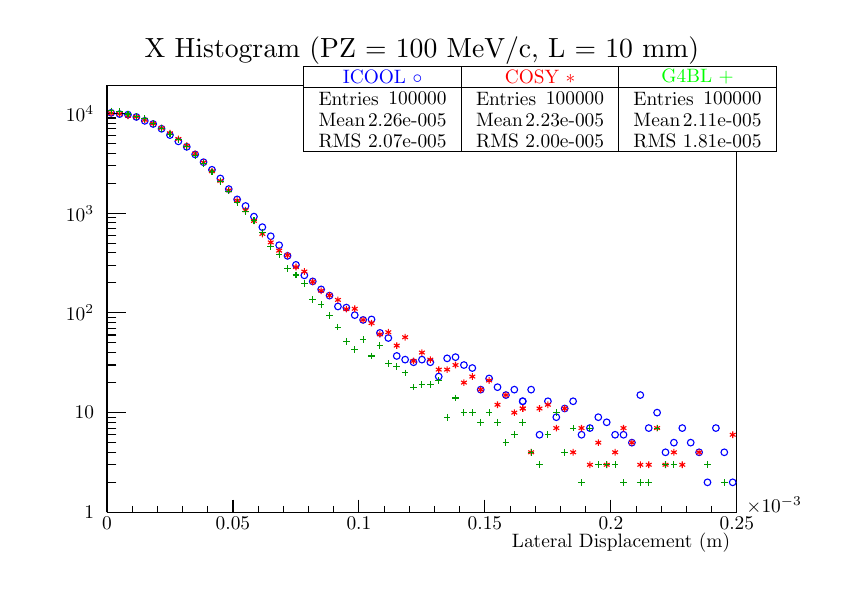
\begin{tikzpicture}
\definecolor{c}{rgb}{1,1,1};
\draw [color=c, fill=c] (0,0) rectangle (20,13.5632);
\draw [color=c, fill=c] (2,1.35632) rectangle (18,12.2069);
\definecolor{c}{rgb}{0,0,0};
\draw [c] (2,1.35632) -- (2,12.2069) -- (18,12.2069) -- (18,1.35632) -- (2,1.35632);
\definecolor{c}{rgb}{1,1,1};
\draw [color=c, fill=c] (2,1.35632) rectangle (18,12.2069);
\definecolor{c}{rgb}{0,0,0};
\draw [c] (2,1.35632) -- (2,12.2069) -- (18,12.2069) -- (18,1.35632) -- (2,1.35632);
\definecolor{c}{rgb}{0,0,1};
\foreach \P in
 {(2.10667,11.5038),(2.32,11.4728),(2.53333,11.4576),(2.74667,11.3996),(2.96,11.3006),(3.17333,11.221),(3.38667,11.099),(3.6,10.9398),(3.81333,10.7796),(4.02667,10.6406),(4.24,10.4467),(4.45333,10.2506),(4.66667,10.058),(4.88,9.83729),(5.09333,9.5678
4),(5.30667,9.3055),(5.52,9.13804),(5.73333,8.8678),(5.94667,8.60064),(6.16,8.36986),(6.37333,8.14157),(6.58667,7.871),(6.8,7.64234),(7.01333,7.37669),(7.22667,7.22316),(7.44,7.01939),(7.65333,6.86146),(7.86667,6.58603),(8.08,6.5572),(8.29333,6.36631
),(8.50667,6.24395),(8.72,6.25681),(8.93333,5.91443),(9.14667,5.78485),(9.36,5.32891),(9.57333,5.23588),(9.78667,5.16918),(10,5.23588),(10.2133,5.16918),(10.4267,4.80586),(10.64,5.26777),(10.8533,5.29876),(11.0667,5.09818),(11.28,5.02228),(11.4933,4.
47331),(11.7067,4.75696),(11.92,4.53619),(12.1333,4.33561),(12.3467,4.47331),(12.56,4.17817)}{\draw[mark options={color=c,fill=c},mark size=2.402402pt,mark=o] plot coordinates {\P};}
\foreach \P in
 {(12.56,4.17817),(12.7733,4.47331),(12.9867,3.32754),(13.2,4.17817),(13.4133,3.77362),(13.6267,3.99439),(13.84,4.17817),(14.0533,3.32754),(14.2667,3.49713),(14.48,3.77362),(14.6933,3.64404),(14.9067,3.32754),(15.12,3.32754),(15.3333,3.12696),(15.546
7,4.33561),(15.76,3.49713),(15.9733,3.88953),(16.1867,2.88147),(16.4,3.12696),(16.6133,3.49713),(16.8267,3.12696),(17.04,2.88147),(17.2533,2.11889),(17.4667,3.49713),(17.68,2.88147),(17.8933,2.11889)}{\draw[mark options={color=c,fill=c},mark
 size=2.402402pt,mark=o] plot coordinates {\P};}
\definecolor{c}{rgb}{1,1,1};
\draw [color=c, fill=c] (7,10.5115) rectangle (11,12.6816);
\definecolor{c}{rgb}{0,0,0};
\draw [c] (7,10.5115) -- (11,10.5115);
\draw [c] (11,10.5115) -- (11,12.6816);
\draw [c] (11,12.6816) -- (7,12.6816);
\draw [c] (7,12.6816) -- (7,10.5115);
\draw[color=blue](9,12.4103) node[scale=0.7, rotate=0]{ICOOL $\circ$};
\draw [c] (7,12.1391) -- (11,12.1391);
\draw [anchor= west] (7.2,11.8678) node[scale=0.7, rotate=0]{Entries };
\draw [anchor= east] (10.8,11.8678) node[scale=0.7, rotate=0]{ 100000};
\draw [anchor= west] (7.2,11.3253) node[scale=0.7, rotate=0]{Mean  };
\draw [anchor= east] (10.8,11.3253) node[scale=0.7, rotate=0]{ 2.26e-005};
\draw [anchor= west] (7.2,10.7828) node[scale=0.7, rotate=0]{RMS   };
\draw [anchor= east] (10.8,10.7828) node[scale=0.7, rotate=0]{ 2.07e-005};
\draw [c] (2,1.35632) -- (18,1.35632);
\draw [anchor= east] (18,0.596782) node[scale=0.7, rotate=0]{Lateral Displacement (m)};
\draw [c] (2,1.68184) -- (2,1.35632);
\draw [c] (2.64,1.51908) -- (2.64,1.35632);
\draw [c] (3.28,1.51908) -- (3.28,1.35632);
\draw [c] (3.92,1.51908) -- (3.92,1.35632);
\draw [c] (4.56,1.51908) -- (4.56,1.35632);
\draw [c] (5.2,1.68184) -- (5.2,1.35632);
\draw [c] (5.84,1.51908) -- (5.84,1.35632);
\draw [c] (6.48,1.51908) -- (6.48,1.35632);
\draw [c] (7.12,1.51908) -- (7.12,1.35632);
\draw [c] (7.76,1.51908) -- (7.76,1.35632);
\draw [c] (8.4,1.68184) -- (8.4,1.35632);
\draw [c] (9.04,1.51908) -- (9.04,1.35632);
\draw [c] (9.68,1.51908) -- (9.68,1.35632);
\draw [c] (10.32,1.51908) -- (10.32,1.35632);
\draw [c] (10.96,1.51908) -- (10.96,1.35632);
\draw [c] (11.6,1.68184) -- (11.6,1.35632);
\draw [c] (12.24,1.51908) -- (12.24,1.35632);
\draw [c] (12.88,1.51908) -- (12.88,1.35632);
\draw [c] (13.52,1.51908) -- (13.52,1.35632);
\draw [c] (14.16,1.51908) -- (14.16,1.35632);
\draw [c] (14.8,1.68184) -- (14.8,1.35632);
\draw [c] (15.44,1.51908) -- (15.44,1.35632);
\draw [c] (16.08,1.51908) -- (16.08,1.35632);
\draw [c] (16.72,1.51908) -- (16.72,1.35632);
\draw [c] (17.36,1.51908) -- (17.36,1.35632);
\draw [c] (18,1.68184) -- (18,1.35632);
\draw [anchor=base] (2,0.908736) node[scale=0.7, rotate=0]{0};
\draw [anchor=base] (5.2,0.908736) node[scale=0.7, rotate=0]{0.05};
\draw [anchor=base] (8.4,0.908736) node[scale=0.7, rotate=0]{0.1};
\draw [anchor=base] (11.6,0.908736) node[scale=0.7, rotate=0]{0.15};
\draw [anchor=base] (14.8,0.908736) node[scale=0.7, rotate=0]{0.2};
\draw [anchor=base] (18,0.908736) node[scale=0.7, rotate=0]{0.25};
\draw [anchor=base west] (18.07,1.35632) node[scale=0.7, rotate=0]{$\times10^{-3}$};
\draw [c] (2,1.35632) -- (2,12.2069);
\draw [c] (2.48,1.35632) -- (2,1.35632);
\draw [anchor= east] (1.844,1.35632) node[scale=0.7, rotate=0]{1};
\draw [c] (2.24,2.1189) -- (2,2.1189);
\draw [c] (2.24,2.56497) -- (2,2.56497);
\draw [c] (2.24,2.88147) -- (2,2.88147);
\draw [c] (2.24,3.12696) -- (2,3.12696);
\draw [c] (2.24,3.32754) -- (2,3.32754);
\draw [c] (2.24,3.49713) -- (2,3.49713);
\draw [c] (2.24,3.64404) -- (2,3.64404);
\draw [c] (2.24,3.77362) -- (2,3.77362);
\draw [c] (2.48,3.88953) -- (2,3.88953);
\draw [anchor= east] (1.844,3.88953) node[scale=0.7, rotate=0]{10};
\draw [c] (2.24,4.65211) -- (2,4.65211);
\draw [c] (2.24,5.09818) -- (2,5.09818);
\draw [c] (2.24,5.41468) -- (2,5.41468);
\draw [c] (2.24,5.66017) -- (2,5.66017);
\draw [c] (2.24,5.86075) -- (2,5.86075);
\draw [c] (2.24,6.03034) -- (2,6.03034);
\draw [c] (2.24,6.17725) -- (2,6.17725);
\draw [c] (2.24,6.30683) -- (2,6.30683);
\draw [c] (2.48,6.42274) -- (2,6.42274);
\draw [anchor= east] (1.844,6.42274) node[scale=0.7, rotate=0]{$10^{2}$};
\draw [c] (2.24,7.18532) -- (2,7.18532);
\draw [c] (2.24,7.63139) -- (2,7.63139);
\draw [c] (2.24,7.94789) -- (2,7.94789);
\draw [c] (2.24,8.19338) -- (2,8.19338);
\draw [c] (2.24,8.39396) -- (2,8.39396);
\draw [c] (2.24,8.56355) -- (2,8.56355);
\draw [c] (2.24,8.71046) -- (2,8.71046);
\draw [c] (2.24,8.84004) -- (2,8.84004);
\draw [c] (2.48,8.95595) -- (2,8.95595);
\draw [anchor= east] (1.844,8.95595) node[scale=0.7, rotate=0]{$10^{3}$};
\draw [c] (2.24,9.71852) -- (2,9.71852);
\draw [c] (2.24,10.1646) -- (2,10.1646);
\draw [c] (2.24,10.4811) -- (2,10.4811);
\draw [c] (2.24,10.7266) -- (2,10.7266);
\draw [c] (2.24,10.9272) -- (2,10.9272);
\draw [c] (2.24,11.0968) -- (2,11.0968);
\draw [c] (2.24,11.2437) -- (2,11.2437);
\draw [c] (2.24,11.3732) -- (2,11.3732);
\draw [c] (2.48,11.4892) -- (2,11.4892);
\draw [anchor= east] (1.844,11.4892) node[scale=0.7, rotate=0]{$10^{4}$};
\definecolor{c}{rgb}{1,1,1};
\draw [color=c, fill=c] (7,10.5115) rectangle (11,12.6816);
\definecolor{c}{rgb}{0,0,0};
\draw [c] (7,10.5115) -- (11,10.5115);
\draw [c] (11,10.5115) -- (11,12.6816);
\draw [c] (11,12.6816) -- (7,12.6816);
\draw [c] (7,12.6816) -- (7,10.5115);
\draw[color=blue](9,12.4103) node[scale=0.7, rotate=0]{ICOOL $\circ$};
\draw [c] (7,12.1391) -- (11,12.1391);
\draw [anchor= west] (7.2,11.8678) node[scale=0.7, rotate=0]{Entries };
\draw [anchor= east] (10.8,11.8678) node[scale=0.7, rotate=0]{ 100000};
\draw [anchor= west] (7.2,11.3253) node[scale=0.7, rotate=0]{Mean  };
\draw [anchor= east] (10.8,11.3253) node[scale=0.7, rotate=0]{ 2.26e-005};
\draw [anchor= west] (7.2,10.7828) node[scale=0.7, rotate=0]{RMS   };
\draw [anchor= east] (10.8,10.7828) node[scale=0.7, rotate=0]{ 2.07e-005};
\draw (10,13.0816) node[scale=1, rotate=0]{X Histogram (PZ = 100 MeV/c, L = 10 mm)};
\definecolor{c}{rgb}{1,0,0};
\foreach \P in
 {(2.10667,11.4927),(2.32,11.4767),(2.53333,11.4308),(2.74667,11.4037),(2.96,11.325),(3.17333,11.2298),(3.38667,11.1173),(3.6,10.9864),(3.81333,10.8408),(4.02667,10.6688),(4.24,10.4692),(4.45333,10.2431),(4.66667,10.021),(4.88,9.77586),(5.09333,9.534
54),(5.30667,9.27629),(5.52,9.02833),(5.73333,8.7602),(5.94667,8.42826),(6.16,8.21301),(6.37333,8.00418),(6.58667,7.88856),(6.8,7.58648),(7.01333,7.47396),(7.22667,7.21248),(7.44,6.98693),(7.65333,6.86882),(7.86667,6.7529),(8.08,6.51755),(8.29333,6.5
276),(8.50667,6.24395),(8.72,6.16341),(8.93333,5.87894),(9.14667,5.93176),(9.36,5.5921),(9.57333,5.80432),(9.78667,5.20304),(10,5.41468),(10.2133,5.23588),(10.4267,4.98227),(10.64,4.98227),(10.8533,5.09818),(11.0667,4.6521),(11.28,4.80586),(11.4933,4
.47331),(11.7067,4.70578),(11.92,4.09011),(12.1333,4.33561),(12.3467,3.88953),(12.56,3.99439)}{\draw[mark options={color=c,fill=c},mark size=2.402402pt,mark=asterisk] plot coordinates {\P};}
\foreach \P in
 {(12.56,3.99439),(12.7733,2.88147),(12.9867,3.99439),(13.2,4.09011),(13.4133,3.49713),(13.6267,3.99439),(13.84,2.88147),(14.0533,3.49713),(14.2667,2.56497),(14.48,3.12696),(14.6933,2.56497),(14.9067,2.88147),(15.12,3.49713),(15.3333,3.12696),(15.546
7,2.56497),(15.76,2.56497),(15.9733,3.49713),(16.1867,2.56497),(16.4,2.88147),(16.6133,2.56497),(17.04,2.88147),(17.8933,3.32754)}{\draw[mark options={color=c,fill=c},mark size=2.402402pt,mark=asterisk] plot coordinates {\P};}
\definecolor{c}{rgb}{1,1,1};
\draw [color=c, fill=c] (11,10.5115) rectangle (15,12.6816);
\definecolor{c}{rgb}{0,0,0};
\draw [c] (11,10.5115) -- (15,10.5115);
\draw [c] (15,10.5115) -- (15,12.6816);
\draw [c] (15,12.6816) -- (11,12.6816);
\draw [c] (11,12.6816) -- (11,10.5115);
\draw [color=red](13,12.4103) node[scale=0.7, rotate=0]{COSY $*$};
\draw [c] (11,12.1391) -- (15,12.1391);
\draw [anchor= west] (11.2,11.8678) node[scale=0.7, rotate=0]{Entries };
\draw [anchor= east] (14.8,11.8678) node[scale=0.7, rotate=0]{ 100000};
\draw [anchor= west] (11.2,11.3253) node[scale=0.7, rotate=0]{Mean  };
\draw [anchor= east] (14.8,11.3253) node[scale=0.7, rotate=0]{ 2.23e-005};
\draw [anchor= west] (11.2,10.7828) node[scale=0.7, rotate=0]{RMS   };
\draw [anchor= east] (14.8,10.7828) node[scale=0.7, rotate=0]{ 2.00e-005};
\definecolor{c}{rgb}{1,1,1};
\draw [color=c, fill=c] (11,10.5115) rectangle (15,12.6816);
\definecolor{c}{rgb}{0,0,0};
\draw [c] (11,10.5115) -- (15,10.5115);
\draw [c] (15,10.5115) -- (15,12.6816);
\draw [c] (15,12.6816) -- (11,12.6816);
\draw [c] (11,12.6816) -- (11,10.5115);
\draw [color=red](13,12.4103) node[scale=0.7, rotate=0]{COSY $*$};
\draw [c] (11,12.1391) -- (15,12.1391);
\draw [anchor= west] (11.2,11.8678) node[scale=0.7, rotate=0]{Entries };
\draw [anchor= east] (14.8,11.8678) node[scale=0.7, rotate=0]{ 100000};
\draw [anchor= west] (11.2,11.3253) node[scale=0.7, rotate=0]{Mean  };
\draw [anchor= east] (14.8,11.3253) node[scale=0.7, rotate=0]{ 2.23e-005};
\draw [anchor= west] (11.2,10.7828) node[scale=0.7, rotate=0]{RMS   };
\draw [anchor= east] (14.8,10.7828) node[scale=0.7, rotate=0]{ 2.00e-005};
\definecolor{c}{rgb}{0,0.6,0};
\foreach \P in
 {(2.10667,11.5526),(2.32,11.5308),(2.53333,11.475),(2.74667,11.4172),(2.96,11.36),(3.17333,11.2255),(3.38667,11.1079),(3.6,10.965),(3.81333,10.8155),(4.02667,10.6479),(4.24,10.4142),(4.45333,10.2207),(4.66667,10.005),(4.88,9.76167),(5.09333,9.51486)
,(5.30667,9.21891),(5.52,8.99167),(5.73333,8.76936),(5.94667,8.47182),(6.16,8.09925),(6.37333,7.90011),(6.58667,7.55155),(6.8,7.3859),(7.01333,7.16309),(7.22667,6.76102),(7.44,6.64151),(7.65333,6.35467),(7.86667,6.06134),(8.08,5.70332),(8.29333,5.494
24),(8.50667,5.74484),(8.72,5.32891),(8.93333,5.5921),(9.14667,5.13425),(9.36,5.06088),(9.57333,4.8976),(9.78667,4.53619),(10,4.59567),(10.2133,4.59567),(10.4267,4.70578),(10.64,3.77362),(10.8533,4.25971),(11.0667,3.88953),(11.28,3.88953),(11.4933,3.
64404),(11.7067,3.88953),(11.92,3.64404),(12.1333,3.12696),(12.3467,3.32754),(12.56,3.64404)}{\draw[mark options={color=c,fill=c},mark size=2.402402pt,mark=+] plot coordinates {\P};}
\foreach \P in
 {(12.56,3.64404),(12.7733,2.88147),(12.9867,2.56497),(13.2,3.32754),(13.4133,3.88953),(13.6267,2.88147),(13.84,3.49713),(14.0533,2.11889),(14.2667,3.49713),(14.48,2.56497),(14.6933,2.56497),(14.9067,2.56497),(15.12,2.11889),(15.5467,2.11889),(15.76,
2.11889),(15.9733,3.49713),(16.1867,2.56497),(16.4,2.56497),(17.2533,2.56497),(17.68,2.11889)}{\draw[mark options={color=c,fill=c},mark size=2.402402pt,mark=+] plot coordinates {\P};}
\definecolor{c}{rgb}{1,1,1};
\draw [color=c, fill=c] (15,10.5115) rectangle (19,12.6816);
\definecolor{c}{rgb}{0,0,0};
\draw [c] (15,10.5115) -- (19,10.5115);
\draw [c] (19,10.5115) -- (19,12.6816);
\draw [c] (19,12.6816) -- (15,12.6816);
\draw [c] (15,12.6816) -- (15,10.5115);
\draw [color=green](17,12.4103) node[scale=0.7, rotate=0]{G4BL $+$};
\draw [c] (15,12.1391) -- (19,12.1391);
\draw [anchor= west] (15.2,11.8678) node[scale=0.7, rotate=0]{Entries };
\draw [anchor= east] (18.8,11.8678) node[scale=0.7, rotate=0]{ 100000};
\draw [anchor= west] (15.2,11.3253) node[scale=0.7, rotate=0]{Mean  };
\draw [anchor= east] (18.8,11.3253) node[scale=0.7, rotate=0]{ 2.11e-005};
\draw [anchor= west] (15.2,10.7828) node[scale=0.7, rotate=0]{RMS   };
\draw [anchor= east] (18.8,10.7828) node[scale=0.7, rotate=0]{ 1.81e-005};
\definecolor{c}{rgb}{1,1,1};
\draw [color=c, fill=c] (15,10.5115) rectangle (19,12.6816);
\definecolor{c}{rgb}{0,0,0};
\draw [c] (15,10.5115) -- (19,10.5115);
\draw [c] (19,10.5115) -- (19,12.6816);
\draw [c] (19,12.6816) -- (15,12.6816);
\draw [c] (15,12.6816) -- (15,10.5115);
\draw [color=green](17,12.4103) node[scale=0.7, rotate=0]{G4BL $+$};
\draw [c] (15,12.1391) -- (19,12.1391);
\draw [anchor= west] (15.2,11.8678) node[scale=0.7, rotate=0]{Entries };
\draw [anchor= east] (18.8,11.8678) node[scale=0.7, rotate=0]{ 100000};
\draw [anchor= west] (15.2,11.3253) node[scale=0.7, rotate=0]{Mean  };
\draw [anchor= east] (18.8,11.3253) node[scale=0.7, rotate=0]{ 2.11e-005};
\draw [anchor= west] (15.2,10.7828) node[scale=0.7, rotate=0]{RMS   };
\draw [anchor= east] (18.8,10.7828) node[scale=0.7, rotate=0]{ 1.81e-005};
\end{tikzpicture}
}\\
\frame{    \pgfdeclareplotmark{cross} {
\pgfpathmoveto{\pgfpoint{-0.3\pgfplotmarksize}{\pgfplotmarksize}}
\pgfpathlineto{\pgfpoint{+0.3\pgfplotmarksize}{\pgfplotmarksize}}
\pgfpathlineto{\pgfpoint{+0.3\pgfplotmarksize}{0.3\pgfplotmarksize}}
\pgfpathlineto{\pgfpoint{+1\pgfplotmarksize}{0.3\pgfplotmarksize}}
\pgfpathlineto{\pgfpoint{+1\pgfplotmarksize}{-0.3\pgfplotmarksize}}
\pgfpathlineto{\pgfpoint{+0.3\pgfplotmarksize}{-0.3\pgfplotmarksize}}
\pgfpathlineto{\pgfpoint{+0.3\pgfplotmarksize}{-1.\pgfplotmarksize}}
\pgfpathlineto{\pgfpoint{-0.3\pgfplotmarksize}{-1.\pgfplotmarksize}}
\pgfpathlineto{\pgfpoint{-0.3\pgfplotmarksize}{-0.3\pgfplotmarksize}}
\pgfpathlineto{\pgfpoint{-1.\pgfplotmarksize}{-0.3\pgfplotmarksize}}
\pgfpathlineto{\pgfpoint{-1.\pgfplotmarksize}{0.3\pgfplotmarksize}}
\pgfpathlineto{\pgfpoint{-0.3\pgfplotmarksize}{0.3\pgfplotmarksize}}
\pgfpathclose
\pgfusepathqstroke
}
\pgfdeclareplotmark{cross*} {
\pgfpathmoveto{\pgfpoint{-0.3\pgfplotmarksize}{\pgfplotmarksize}}
\pgfpathlineto{\pgfpoint{+0.3\pgfplotmarksize}{\pgfplotmarksize}}
\pgfpathlineto{\pgfpoint{+0.3\pgfplotmarksize}{0.3\pgfplotmarksize}}
\pgfpathlineto{\pgfpoint{+1\pgfplotmarksize}{0.3\pgfplotmarksize}}
\pgfpathlineto{\pgfpoint{+1\pgfplotmarksize}{-0.3\pgfplotmarksize}}
\pgfpathlineto{\pgfpoint{+0.3\pgfplotmarksize}{-0.3\pgfplotmarksize}}
\pgfpathlineto{\pgfpoint{+0.3\pgfplotmarksize}{-1.\pgfplotmarksize}}
\pgfpathlineto{\pgfpoint{-0.3\pgfplotmarksize}{-1.\pgfplotmarksize}}
\pgfpathlineto{\pgfpoint{-0.3\pgfplotmarksize}{-0.3\pgfplotmarksize}}
\pgfpathlineto{\pgfpoint{-1.\pgfplotmarksize}{-0.3\pgfplotmarksize}}
\pgfpathlineto{\pgfpoint{-1.\pgfplotmarksize}{0.3\pgfplotmarksize}}
\pgfpathlineto{\pgfpoint{-0.3\pgfplotmarksize}{0.3\pgfplotmarksize}}
\pgfpathclose
\pgfusepathqfillstroke
}
\pgfdeclareplotmark{newstar} {
\pgfpathmoveto{\pgfqpoint{0pt}{\pgfplotmarksize}}
\pgfpathlineto{\pgfqpointpolar{44}{0.5\pgfplotmarksize}}
\pgfpathlineto{\pgfqpointpolar{18}{\pgfplotmarksize}}
\pgfpathlineto{\pgfqpointpolar{-20}{0.5\pgfplotmarksize}}
\pgfpathlineto{\pgfqpointpolar{-54}{\pgfplotmarksize}}
\pgfpathlineto{\pgfqpointpolar{-90}{0.5\pgfplotmarksize}}
\pgfpathlineto{\pgfqpointpolar{234}{\pgfplotmarksize}}
\pgfpathlineto{\pgfqpointpolar{198}{0.5\pgfplotmarksize}}
\pgfpathlineto{\pgfqpointpolar{162}{\pgfplotmarksize}}
\pgfpathlineto{\pgfqpointpolar{134}{0.5\pgfplotmarksize}}
\pgfpathclose
\pgfusepathqstroke
}
\pgfdeclareplotmark{newstar*} {
\pgfpathmoveto{\pgfqpoint{0pt}{\pgfplotmarksize}}
\pgfpathlineto{\pgfqpointpolar{44}{0.5\pgfplotmarksize}}
\pgfpathlineto{\pgfqpointpolar{18}{\pgfplotmarksize}}
\pgfpathlineto{\pgfqpointpolar{-20}{0.5\pgfplotmarksize}}
\pgfpathlineto{\pgfqpointpolar{-54}{\pgfplotmarksize}}
\pgfpathlineto{\pgfqpointpolar{-90}{0.5\pgfplotmarksize}}
\pgfpathlineto{\pgfqpointpolar{234}{\pgfplotmarksize}}
\pgfpathlineto{\pgfqpointpolar{198}{0.5\pgfplotmarksize}}
\pgfpathlineto{\pgfqpointpolar{162}{\pgfplotmarksize}}
\pgfpathlineto{\pgfqpointpolar{134}{0.5\pgfplotmarksize}}
\pgfpathclose
\pgfusepathqfillstroke
}
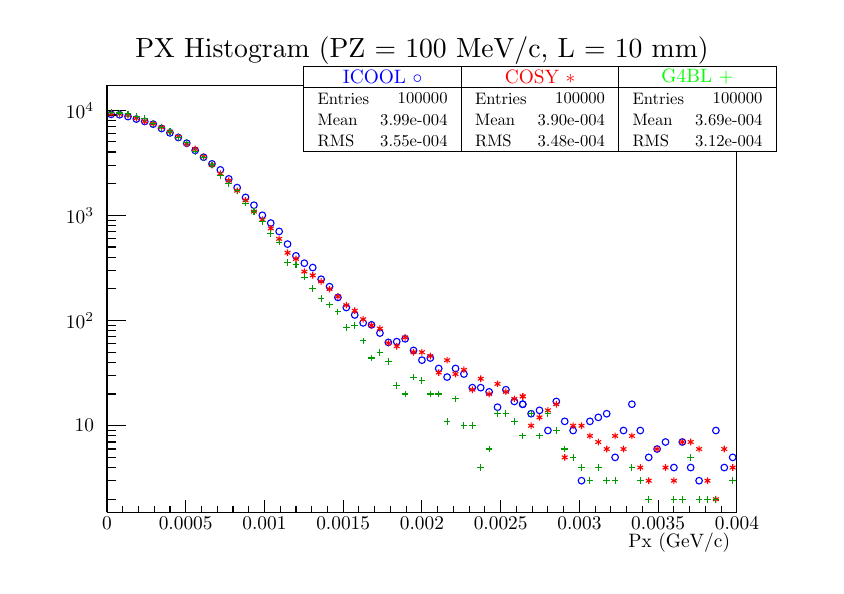
\begin{tikzpicture}
\definecolor{c}{rgb}{1,1,1};
\draw [color=c, fill=c] (0,0) rectangle (20,13.5632);
\draw [color=c, fill=c] (2,1.35632) rectangle (18,12.2069);
\definecolor{c}{rgb}{0,0,0};
\draw [c] (2,1.35632) -- (2,12.2069) -- (18,12.2069) -- (18,1.35632) -- (2,1.35632);
\definecolor{c}{rgb}{1,1,1};
\draw [color=c, fill=c] (2,1.35632) rectangle (18,12.2069);
\definecolor{c}{rgb}{0,0,0};
\draw [c] (2,1.35632) -- (2,12.2069) -- (18,12.2069) -- (18,1.35632) -- (2,1.35632);
\definecolor{c}{rgb}{0,0,1};
\foreach \P in
 {(2.10667,11.4655),(2.32,11.4562),(2.53333,11.4095),(2.74667,11.3462),(2.96,11.2846),(3.17333,11.2164),(3.38667,11.1056),(3.6,10.9953),(3.81333,10.8773),(4.02667,10.7323),(4.24,10.5499),(4.45333,10.3768),(4.66667,10.2075),(4.88,10.0551),(5.09333,9.8
2604),(5.30667,9.60467),(5.52,9.35618),(5.73333,9.15774),(5.94667,8.90211),(6.16,8.7044),(6.37333,8.49261),(6.58667,8.1698),(6.8,7.87107),(7.01333,7.68518),(7.22667,7.57427),(7.44,7.27751),(7.65333,7.08924),(7.86667,6.81648),(8.08,6.55935),(8.29333,6
.37029),(8.50667,6.169),(8.72,6.11909),(8.93333,5.91012),(9.14667,5.67392),(9.36,5.69249),(9.57333,5.7639),(9.78667,5.46987),(10,5.2221),(10.2133,5.27606),(10.4267,5.01058),(10.64,4.79242),(10.8533,5.01058),(11.0667,4.86979),(11.28,4.5235),(11.4933,4
.5235),(11.7067,4.41796),(11.92,4.02761),(12.1333,4.47193),(12.3467,4.17281),(12.56,4.10248)}{\draw[mark options={color=c,fill=c},mark size=2.402402pt,mark=o] plot coordinates {\P};}
\foreach \P in
 {(12.56,4.10248),(12.7733,3.86159),(12.9867,3.94757),(13.2,3.43499),(13.4133,4.17281),(13.6267,3.66779),(13.84,3.43499),(14.0533,2.16046),(14.2667,3.66779),(14.48,3.76873),(14.6933,3.86159),(14.9067,2.75308),(15.12,3.43499),(15.3333,4.10248),(15.546
7,3.43499),(15.76,2.75308),(15.9733,2.9646),(16.1867,3.14343),(16.4,2.49421),(16.6133,3.14343),(16.8267,2.49421),(17.04,2.16046),(17.4667,3.43499),(17.68,2.49421),(17.8933,2.75308)}{\draw[mark options={color=c,fill=c},mark size=2.402402pt,mark=o]
 plot coordinates {\P};}
\definecolor{c}{rgb}{1,1,1};
\draw [color=c, fill=c] (7,10.5115) rectangle (11,12.6816);
\definecolor{c}{rgb}{0,0,0};
\draw [c] (7,10.5115) -- (11,10.5115);
\draw [c] (11,10.5115) -- (11,12.6816);
\draw [c] (11,12.6816) -- (7,12.6816);
\draw [c] (7,12.6816) -- (7,10.5115);
\draw[color=blue](9,12.4103) node[scale=0.7, rotate=0]{ICOOL $\circ$};
\draw [c] (7,12.1391) -- (11,12.1391);
\draw [anchor= west] (7.2,11.8678) node[scale=0.6, rotate=0]{Entries };
\draw [anchor= east] (10.8,11.8678) node[scale=0.6, rotate=0]{ 100000};
\draw [anchor= west] (7.2,11.3253) node[scale=0.6, rotate=0]{Mean  };
\draw [anchor= east] (10.8,11.3253) node[scale=0.6, rotate=0]{ 3.99e-004};
\draw [anchor= west] (7.2,10.7828) node[scale=0.6, rotate=0]{RMS   };
\draw [anchor= east] (10.8,10.7828) node[scale=0.6, rotate=0]{ 3.55e-004};
\draw [c] (2,1.35632) -- (18,1.35632);
\draw [anchor= east] (18,0.596782) node[scale=0.7, rotate=0]{Px (GeV/c)};
\draw [c] (2,1.68184) -- (2,1.35632);
\draw [c] (2.4,1.51908) -- (2.4,1.35632);
\draw [c] (2.8,1.51908) -- (2.8,1.35632);
\draw [c] (3.2,1.51908) -- (3.2,1.35632);
\draw [c] (3.6,1.51908) -- (3.6,1.35632);
\draw [c] (4,1.68184) -- (4,1.35632);
\draw [c] (4.4,1.51908) -- (4.4,1.35632);
\draw [c] (4.8,1.51908) -- (4.8,1.35632);
\draw [c] (5.2,1.51908) -- (5.2,1.35632);
\draw [c] (5.6,1.51908) -- (5.6,1.35632);
\draw [c] (6,1.68184) -- (6,1.35632);
\draw [c] (6.4,1.51908) -- (6.4,1.35632);
\draw [c] (6.8,1.51908) -- (6.8,1.35632);
\draw [c] (7.2,1.51908) -- (7.2,1.35632);
\draw [c] (7.6,1.51908) -- (7.6,1.35632);
\draw [c] (8,1.68184) -- (8,1.35632);
\draw [c] (8.4,1.51908) -- (8.4,1.35632);
\draw [c] (8.8,1.51908) -- (8.8,1.35632);
\draw [c] (9.2,1.51908) -- (9.2,1.35632);
\draw [c] (9.6,1.51908) -- (9.6,1.35632);
\draw [c] (10,1.68184) -- (10,1.35632);
\draw [c] (10.4,1.51908) -- (10.4,1.35632);
\draw [c] (10.8,1.51908) -- (10.8,1.35632);
\draw [c] (11.2,1.51908) -- (11.2,1.35632);
\draw [c] (11.6,1.51908) -- (11.6,1.35632);
\draw [c] (12,1.68184) -- (12,1.35632);
\draw [c] (12.4,1.51908) -- (12.4,1.35632);
\draw [c] (12.8,1.51908) -- (12.8,1.35632);
\draw [c] (13.2,1.51908) -- (13.2,1.35632);
\draw [c] (13.6,1.51908) -- (13.6,1.35632);
\draw [c] (14,1.68184) -- (14,1.35632);
\draw [c] (14.4,1.51908) -- (14.4,1.35632);
\draw [c] (14.8,1.51908) -- (14.8,1.35632);
\draw [c] (15.2,1.51908) -- (15.2,1.35632);
\draw [c] (15.6,1.51908) -- (15.6,1.35632);
\draw [c] (16,1.68184) -- (16,1.35632);
\draw [c] (16.4,1.51908) -- (16.4,1.35632);
\draw [c] (16.8,1.51908) -- (16.8,1.35632);
\draw [c] (17.2,1.51908) -- (17.2,1.35632);
\draw [c] (17.6,1.51908) -- (17.6,1.35632);
\draw [c] (18,1.68184) -- (18,1.35632);
\draw [anchor=base] (2,0.908736) node[scale=0.7, rotate=0]{0};
\draw [anchor=base] (4,0.908736) node[scale=0.7, rotate=0]{0.0005};
\draw [anchor=base] (6,0.908736) node[scale=0.7, rotate=0]{0.001};
\draw [anchor=base] (8,0.908736) node[scale=0.7, rotate=0]{0.0015};
\draw [anchor=base] (10,0.908736) node[scale=0.7, rotate=0]{0.002};
\draw [anchor=base] (12,0.908736) node[scale=0.7, rotate=0]{0.0025};
\draw [anchor=base] (14,0.908736) node[scale=0.7, rotate=0]{0.003};
\draw [anchor=base] (16,0.908736) node[scale=0.7, rotate=0]{0.0035};
\draw [anchor=base] (18,0.908736) node[scale=0.7, rotate=0]{0.004};
\draw [c] (2,1.35632) -- (2,12.2069);
\draw [c] (2.24,1.69007) -- (2,1.69007);
\draw [c] (2.24,2.16046) -- (2,2.16046);
\draw [c] (2.24,2.4942) -- (2,2.4942);
\draw [c] (2.24,2.75308) -- (2,2.75308);
\draw [c] (2.24,2.96459) -- (2,2.96459);
\draw [c] (2.24,3.14343) -- (2,3.14343);
\draw [c] (2.24,3.29834) -- (2,3.29834);
\draw [c] (2.24,3.43498) -- (2,3.43498);
\draw [c] (2.48,3.55722) -- (2,3.55722);
\draw [anchor= east] (1.844,3.55722) node[scale=0.7, rotate=0]{10};
\draw [c] (2.24,4.36135) -- (2,4.36135);
\draw [c] (2.24,4.83174) -- (2,4.83174);
\draw [c] (2.24,5.16549) -- (2,5.16549);
\draw [c] (2.24,5.42437) -- (2,5.42437);
\draw [c] (2.24,5.63588) -- (2,5.63588);
\draw [c] (2.24,5.81472) -- (2,5.81472);
\draw [c] (2.24,5.96963) -- (2,5.96963);
\draw [c] (2.24,6.10627) -- (2,6.10627);
\draw [c] (2.48,6.2285) -- (2,6.2285);
\draw [anchor= east] (1.844,6.2285) node[scale=0.7, rotate=0]{$10^{2}$};
\draw [c] (2.24,7.03264) -- (2,7.03264);
\draw [c] (2.24,7.50303) -- (2,7.50303);
\draw [c] (2.24,7.83678) -- (2,7.83678);
\draw [c] (2.24,8.09565) -- (2,8.09565);
\draw [c] (2.24,8.30717) -- (2,8.30717);
\draw [c] (2.24,8.486) -- (2,8.486);
\draw [c] (2.24,8.64092) -- (2,8.64092);
\draw [c] (2.24,8.77756) -- (2,8.77756);
\draw [c] (2.48,8.89979) -- (2,8.89979);
\draw [anchor= east] (1.844,8.89979) node[scale=0.7, rotate=0]{$10^{3}$};
\draw [c] (2.24,9.70393) -- (2,9.70393);
\draw [c] (2.24,10.1743) -- (2,10.1743);
\draw [c] (2.24,10.5081) -- (2,10.5081);
\draw [c] (2.24,10.7669) -- (2,10.7669);
\draw [c] (2.24,10.9785) -- (2,10.9785);
\draw [c] (2.24,11.1573) -- (2,11.1573);
\draw [c] (2.24,11.3122) -- (2,11.3122);
\draw [c] (2.24,11.4488) -- (2,11.4488);
\draw [c] (2.48,11.5711) -- (2,11.5711);
\draw [anchor= east] (1.844,11.5711) node[scale=0.7, rotate=0]{$10^{4}$};
\definecolor{c}{rgb}{1,1,1};
\draw [color=c, fill=c] (7,10.5115) rectangle (11,12.6816);
\definecolor{c}{rgb}{0,0,0};
\draw [c] (7,10.5115) -- (11,10.5115);
\draw [c] (11,10.5115) -- (11,12.6816);
\draw [c] (11,12.6816) -- (7,12.6816);
\draw [c] (7,12.6816) -- (7,10.5115);
\draw[color=blue](9,12.4103) node[scale=0.7, rotate=0]{ICOOL $\circ$};
\draw [c] (7,12.1391) -- (11,12.1391);
\draw [anchor= west] (7.2,11.8678) node[scale=0.6, rotate=0]{Entries };
\draw [anchor= east] (10.8,11.8678) node[scale=0.6, rotate=0]{ 100000};
\draw [anchor= west] (7.2,11.3253) node[scale=0.6, rotate=0]{Mean  };
\draw [anchor= east] (10.8,11.3253) node[scale=0.6, rotate=0]{ 3.99e-004};
\draw [anchor= west] (7.2,10.7828) node[scale=0.6, rotate=0]{RMS   };
\draw [anchor= east] (10.8,10.7828) node[scale=0.6, rotate=0]{ 3.55e-004};
\draw (10,13.0816) node[scale=1, rotate=0]{PX Histogram (PZ = 100 MeV/c, L = 10 mm)};
\definecolor{c}{rgb}{1,0,0};
\foreach \P in
 {(2.10667,11.483),(2.32,11.4764),(2.53333,11.4454),(2.74667,11.3683),(2.96,11.2902),(3.17333,11.226),(3.38667,11.1369),(3.6,11.0253),(3.81333,10.8995),(4.02667,10.7167),(4.24,10.586),(4.45333,10.3897),(4.66667,10.1786),(4.88,9.95908),(5.09333,9.7813
4),(5.30667,9.52693),(5.52,9.28099),(5.73333,8.9955),(5.94667,8.78783),(6.16,8.56913),(6.37333,8.3033),(6.58667,7.94998),(6.8,7.79545),(7.01333,7.47168),(7.22667,7.3765),(7.44,7.21973),(7.65333,7.02683),(7.86667,6.83726),(8.08,6.61885),(8.29333,6.478
06),(8.50667,6.2628),(8.72,6.10627),(8.93333,6.02623),(9.14667,5.65506),(9.36,5.57638),(9.57333,5.79802),(9.78667,5.42437),(10,5.42437),(10.2133,5.32763),(10.4267,4.90662),(10.64,5.2221),(10.8533,4.86979),(11.0667,4.97695),(11.28,4.47193),(11.4933,4.
75171),(11.7067,4.36136),(11.92,4.62023),(12.1333,4.41796),(12.3467,4.23912),(12.56,4.30185)}{\draw[mark options={color=c,fill=c},mark size=2.402402pt,mark=asterisk] plot coordinates {\P};}
\foreach \P in
 {(12.56,4.30185),(12.7733,3.55722),(12.9867,3.76873),(13.2,3.94757),(13.4133,4.10248),(13.6267,2.75308),(13.84,3.55722),(14.0533,3.55722),(14.2667,3.29834),(14.48,3.14343),(14.6933,2.9646),(14.9067,3.29834),(15.12,2.9646),(15.3333,3.29834),(15.5467,
2.49421),(15.76,2.16046),(15.9733,2.9646),(16.1867,2.49421),(16.4,2.16046),(16.6133,3.14343),(16.8267,3.14343),(17.04,2.9646),(17.2533,2.16046),(17.4667,1.69007),(17.68,2.9646),(17.8933,2.49421)}{\draw[mark options={color=c,fill=c},mark
 size=2.402402pt,mark=asterisk] plot coordinates {\P};}
\definecolor{c}{rgb}{1,1,1};
\draw [color=c, fill=c] (11,10.5115) rectangle (15,12.6816);
\definecolor{c}{rgb}{0,0,0};
\draw [c] (11,10.5115) -- (15,10.5115);
\draw [c] (15,10.5115) -- (15,12.6816);
\draw [c] (15,12.6816) -- (11,12.6816);
\draw [c] (11,12.6816) -- (11,10.5115);
\draw [color=red](13,12.4103) node[scale=0.7, rotate=0]{COSY $*$};
\draw [c] (11,12.1391) -- (15,12.1391);
\draw [anchor= west] (11.2,11.8678) node[scale=0.6, rotate=0]{Entries };
\draw [anchor= east] (14.8,11.8678) node[scale=0.6, rotate=0]{ 100000};
\draw [anchor= west] (11.2,11.3253) node[scale=0.6, rotate=0]{Mean  };
\draw [anchor= east] (14.8,11.3253) node[scale=0.6, rotate=0]{ 3.90e-004};
\draw [anchor= west] (11.2,10.7828) node[scale=0.6, rotate=0]{RMS   };
\draw [anchor= east] (14.8,10.7828) node[scale=0.6, rotate=0]{ 3.48e-004};
\definecolor{c}{rgb}{1,1,1};
\draw [color=c, fill=c] (11,10.5115) rectangle (15,12.6816);
\definecolor{c}{rgb}{0,0,0};
\draw [c] (11,10.5115) -- (15,10.5115);
\draw [c] (15,10.5115) -- (15,12.6816);
\draw [c] (15,12.6816) -- (11,12.6816);
\draw [c] (11,12.6816) -- (11,10.5115);
\draw [color=red](13,12.4103) node[scale=0.7, rotate=0]{COSY $*$};
\draw [c] (11,12.1391) -- (15,12.1391);
\draw [anchor= west] (11.2,11.8678) node[scale=0.6, rotate=0]{Entries };
\draw [anchor= east] (14.8,11.8678) node[scale=0.6, rotate=0]{ 100000};
\draw [anchor= west] (11.2,11.3253) node[scale=0.6, rotate=0]{Mean  };
\draw [anchor= east] (14.8,11.3253) node[scale=0.6, rotate=0]{ 3.90e-004};
\draw [anchor= west] (11.2,10.7828) node[scale=0.6, rotate=0]{RMS   };
\draw [anchor= east] (14.8,10.7828) node[scale=0.6, rotate=0]{ 3.48e-004};
\definecolor{c}{rgb}{0,0.6,0};
\foreach \P in
 {(2.10667,11.5213),(2.32,11.4989),(2.53333,11.4789),(2.74667,11.4136),(2.96,11.3569),(3.17333,11.2308),(3.38667,11.1369),(3.6,11.0332),(3.81333,10.8834),(4.02667,10.7539),(4.24,10.5225),(4.45333,10.3771),(4.66667,10.1805),(4.88,9.91882),(5.09333,9.7
0102),(5.30667,9.52287),(5.52,9.21128),(5.73333,8.99443),(5.94667,8.74885),(6.16,8.44381),(6.37333,8.2209),(6.58667,7.70159),(6.8,7.64139),(7.01333,7.33255),(7.22667,7.03843),(7.44,6.79532),(7.65333,6.62711),(7.86667,6.44965),(8.08,6.05353),(8.29333,
6.10627),(8.50667,5.71076),(8.72,5.27606),(8.93333,5.42437),(9.14667,5.19414),(9.36,4.57287),(9.57333,4.36136),(9.78667,4.79242),(10,4.70951),(10.2133,4.36136),(10.4267,4.36136),(10.64,3.66779),(10.8533,4.23912),(11.0667,3.55722),(11.28,3.55722),(11.
4933,2.49421),(11.7067,2.9646),(11.92,3.86159),(12.1333,3.86159),(12.3467,3.66779),(12.56,3.29834)}{\draw[mark options={color=c,fill=c},mark size=2.402402pt,mark=+] plot coordinates {\P};}
\foreach \P in
 {(12.56,3.29834),(12.7733,3.86159),(12.9867,3.29834),(13.2,3.86159),(13.4133,3.43499),(13.6267,2.9646),(13.84,2.75308),(14.0533,2.49421),(14.2667,2.16046),(14.48,2.49421),(14.6933,2.16046),(14.9067,2.16046),(15.3333,2.49421),(15.5467,2.16046),(15.76
,1.69007),(16.4,1.69007),(16.6133,1.69007),(16.8267,2.75308),(17.04,1.69007),(17.2533,1.69007),(17.4667,1.69007),(17.8933,2.16046)}{\draw[mark options={color=c,fill=c},mark size=2.402402pt,mark=+] plot coordinates {\P};}
\definecolor{c}{rgb}{1,1,1};
\draw [color=c, fill=c] (15,10.5115) rectangle (19,12.6816);
\definecolor{c}{rgb}{0,0,0};
\draw [c] (15,10.5115) -- (19,10.5115);
\draw [c] (19,10.5115) -- (19,12.6816);
\draw [c] (19,12.6816) -- (15,12.6816);
\draw [c] (15,12.6816) -- (15,10.5115);
\draw [color=green](17,12.4103) node[scale=0.7, rotate=0]{G4BL $+$};
\draw [c] (15,12.1391) -- (19,12.1391);
\draw [anchor= west] (15.2,11.8678) node[scale=0.6, rotate=0]{Entries };
\draw [anchor= east] (18.8,11.8678) node[scale=0.6, rotate=0]{ 100000};
\draw [anchor= west] (15.2,11.3253) node[scale=0.6, rotate=0]{Mean  };
\draw [anchor= east] (18.8,11.3253) node[scale=0.6, rotate=0]{ 3.69e-004};
\draw [anchor= west] (15.2,10.7828) node[scale=0.6, rotate=0]{RMS   };
\draw [anchor= east] (18.8,10.7828) node[scale=0.6, rotate=0]{ 3.12e-004};
\definecolor{c}{rgb}{1,1,1};
\draw [color=c, fill=c] (15,10.5115) rectangle (19,12.6816);
\definecolor{c}{rgb}{0,0,0};
\draw [c] (15,10.5115) -- (19,10.5115);
\draw [c] (19,10.5115) -- (19,12.6816);
\draw [c] (19,12.6816) -- (15,12.6816);
\draw [c] (15,12.6816) -- (15,10.5115);
\draw [color=green](17,12.4103) node[scale=0.7, rotate=0]{G4BL $+$};
\draw [c] (15,12.1391) -- (19,12.1391);
\draw [anchor= west] (15.2,11.8678) node[scale=0.6, rotate=0]{Entries };
\draw [anchor= east] (18.8,11.8678) node[scale=0.6, rotate=0]{ 100000};
\draw [anchor= west] (15.2,11.3253) node[scale=0.6, rotate=0]{Mean  };
\draw [anchor= east] (18.8,11.3253) node[scale=0.6, rotate=0]{ 3.69e-004};
\draw [anchor= west] (15.2,10.7828) node[scale=0.6, rotate=0]{RMS   };
\draw [anchor= east] (18.8,10.7828) node[scale=0.6, rotate=0]{ 3.12e-004};
\end{tikzpicture}
}\\
\frame{\pgfdeclareplotmark{cross} {
\pgfpathmoveto{\pgfpoint{-0.3\pgfplotmarksize}{\pgfplotmarksize}}
\pgfpathlineto{\pgfpoint{+0.3\pgfplotmarksize}{\pgfplotmarksize}}
\pgfpathlineto{\pgfpoint{+0.3\pgfplotmarksize}{0.3\pgfplotmarksize}}
\pgfpathlineto{\pgfpoint{+1\pgfplotmarksize}{0.3\pgfplotmarksize}}
\pgfpathlineto{\pgfpoint{+1\pgfplotmarksize}{-0.3\pgfplotmarksize}}
\pgfpathlineto{\pgfpoint{+0.3\pgfplotmarksize}{-0.3\pgfplotmarksize}}
\pgfpathlineto{\pgfpoint{+0.3\pgfplotmarksize}{-1.\pgfplotmarksize}}
\pgfpathlineto{\pgfpoint{-0.3\pgfplotmarksize}{-1.\pgfplotmarksize}}
\pgfpathlineto{\pgfpoint{-0.3\pgfplotmarksize}{-0.3\pgfplotmarksize}}
\pgfpathlineto{\pgfpoint{-1.\pgfplotmarksize}{-0.3\pgfplotmarksize}}
\pgfpathlineto{\pgfpoint{-1.\pgfplotmarksize}{0.3\pgfplotmarksize}}
\pgfpathlineto{\pgfpoint{-0.3\pgfplotmarksize}{0.3\pgfplotmarksize}}
\pgfpathclose
\pgfusepathqstroke
}
\pgfdeclareplotmark{cross*} {
\pgfpathmoveto{\pgfpoint{-0.3\pgfplotmarksize}{\pgfplotmarksize}}
\pgfpathlineto{\pgfpoint{+0.3\pgfplotmarksize}{\pgfplotmarksize}}
\pgfpathlineto{\pgfpoint{+0.3\pgfplotmarksize}{0.3\pgfplotmarksize}}
\pgfpathlineto{\pgfpoint{+1\pgfplotmarksize}{0.3\pgfplotmarksize}}
\pgfpathlineto{\pgfpoint{+1\pgfplotmarksize}{-0.3\pgfplotmarksize}}
\pgfpathlineto{\pgfpoint{+0.3\pgfplotmarksize}{-0.3\pgfplotmarksize}}
\pgfpathlineto{\pgfpoint{+0.3\pgfplotmarksize}{-1.\pgfplotmarksize}}
\pgfpathlineto{\pgfpoint{-0.3\pgfplotmarksize}{-1.\pgfplotmarksize}}
\pgfpathlineto{\pgfpoint{-0.3\pgfplotmarksize}{-0.3\pgfplotmarksize}}
\pgfpathlineto{\pgfpoint{-1.\pgfplotmarksize}{-0.3\pgfplotmarksize}}
\pgfpathlineto{\pgfpoint{-1.\pgfplotmarksize}{0.3\pgfplotmarksize}}
\pgfpathlineto{\pgfpoint{-0.3\pgfplotmarksize}{0.3\pgfplotmarksize}}
\pgfpathclose
\pgfusepathqfillstroke
}
\pgfdeclareplotmark{newstar} {
\pgfpathmoveto{\pgfqpoint{0pt}{\pgfplotmarksize}}
\pgfpathlineto{\pgfqpointpolar{44}{0.5\pgfplotmarksize}}
\pgfpathlineto{\pgfqpointpolar{18}{\pgfplotmarksize}}
\pgfpathlineto{\pgfqpointpolar{-20}{0.5\pgfplotmarksize}}
\pgfpathlineto{\pgfqpointpolar{-54}{\pgfplotmarksize}}
\pgfpathlineto{\pgfqpointpolar{-90}{0.5\pgfplotmarksize}}
\pgfpathlineto{\pgfqpointpolar{234}{\pgfplotmarksize}}
\pgfpathlineto{\pgfqpointpolar{198}{0.5\pgfplotmarksize}}
\pgfpathlineto{\pgfqpointpolar{162}{\pgfplotmarksize}}
\pgfpathlineto{\pgfqpointpolar{134}{0.5\pgfplotmarksize}}
\pgfpathclose
\pgfusepathqstroke
}
\pgfdeclareplotmark{newstar*} {
\pgfpathmoveto{\pgfqpoint{0pt}{\pgfplotmarksize}}
\pgfpathlineto{\pgfqpointpolar{44}{0.5\pgfplotmarksize}}
\pgfpathlineto{\pgfqpointpolar{18}{\pgfplotmarksize}}
\pgfpathlineto{\pgfqpointpolar{-20}{0.5\pgfplotmarksize}}
\pgfpathlineto{\pgfqpointpolar{-54}{\pgfplotmarksize}}
\pgfpathlineto{\pgfqpointpolar{-90}{0.5\pgfplotmarksize}}
\pgfpathlineto{\pgfqpointpolar{234}{\pgfplotmarksize}}
\pgfpathlineto{\pgfqpointpolar{198}{0.5\pgfplotmarksize}}
\pgfpathlineto{\pgfqpointpolar{162}{\pgfplotmarksize}}
\pgfpathlineto{\pgfqpointpolar{134}{0.5\pgfplotmarksize}}
\pgfpathclose
\pgfusepathqfillstroke
}
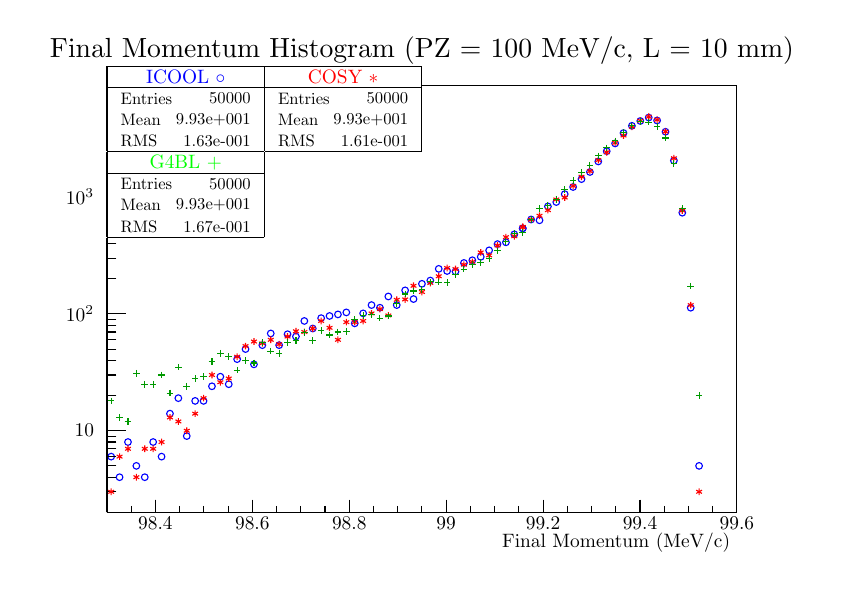
\begin{tikzpicture}
\definecolor{c}{rgb}{1,1,1};
\draw [color=c, fill=c] (0,0) rectangle (20,13.5632);
\draw [color=c, fill=c] (2,1.35632) rectangle (18,12.2069);
\definecolor{c}{rgb}{0,0,0};
\draw [c] (2,1.35632) -- (2,12.2069) -- (18,12.2069) -- (18,1.35632) -- (2,1.35632);
\definecolor{c}{rgb}{1,1,1};
\draw [color=c, fill=c] (2,1.35632) rectangle (18,12.2069);
\definecolor{c}{rgb}{0,0,0};
\draw [c] (2,1.35632) -- (2,12.2069) -- (18,12.2069) -- (18,1.35632) -- (2,1.35632);
\definecolor{c}{rgb}{0,0,1};
\foreach \P in
 {(2.10667,2.77192),(2.32,2.24947),(2.53333,3.14261),(2.74667,2.537),(2.96,2.24947),(3.17333,3.14261),(3.38667,2.77192),(3.6,3.8637),(3.81333,4.2572),(4.02667,3.29438),(4.24,4.18753),(4.45333,4.18753),(4.66667,4.55822),(4.88,4.80206),(5.09333,4.61082
),(5.30667,5.24825),(5.52,5.50396),(5.73333,5.11598),(5.94667,5.60313),(6.16,5.90017),(6.37333,5.60313),(6.58667,5.88108),(6.8,5.82205),(7.01333,6.21767),(7.22667,6.02642),(7.44,6.28967),(7.65333,6.34451),(7.86667,6.38416),(8.08,6.4352),(8.29333,6.15
702),(8.50667,6.40993),(8.72,6.62126),(8.93333,6.55459),(9.14667,6.83984),(9.36,6.62126),(9.57333,6.99465),(9.78667,6.77423),(10,7.16163),(10.2133,7.24435),(10.4267,7.54119),(10.64,7.48704),(10.8533,7.47594),(11.0667,7.69119),(11.28,7.76011),(11.4933
,7.84662),(11.7067,8.01134),(11.92,8.17045),(12.1333,8.21522),(12.3467,8.41833),(12.56,8.5701)}{\draw[mark options={color=c,fill=c},mark size=2.402402pt,mark=o] plot coordinates {\P};}
\foreach \P in
 {(12.56,8.5701),(12.7733,8.79505),(12.9867,8.77485),(13.2,9.12709),(13.4133,9.2383),(13.6267,9.43916),(13.84,9.6203),(14.0533,9.82044),(14.2667,10.0015),(14.48,10.2694),(14.6933,10.5302),(14.9067,10.7271),(15.12,10.9911),(15.3333,11.1746),(15.5467,1
1.2964),(15.76,11.3834),(15.9733,11.3096),(16.1867,11.0235),(16.4,10.2928),(16.6133,8.96736),(16.8267,6.55459),(17.04,2.537)}{\draw[mark options={color=c,fill=c},mark size=2.402402pt,mark=o] plot coordinates {\P};}
\definecolor{c}{rgb}{1,1,1};
\draw [color=c, fill=c] (2,10.5115) rectangle (6,12.6816);
\definecolor{c}{rgb}{0,0,0};
\draw [c] (2,10.5115) -- (6,10.5115);
\draw [c] (6,10.5115) -- (6,12.6816);
\draw [c] (6,12.6816) -- (2,12.6816);
\draw [c] (2,12.6816) -- (2,10.5115);
\draw[color=blue](4,12.4103) node[scale=0.7, rotate=0]{ICOOL $\circ$};
\draw [c] (2,12.1391) -- (6,12.1391);
\draw [anchor= west] (2.2,11.8678) node[scale=0.6, rotate=0]{Entries };
\draw [anchor= east] (5.8,11.8678) node[scale=0.6, rotate=0]{ 50000};
\draw [anchor= west] (2.2,11.3253) node[scale=0.6, rotate=0]{Mean  };
\draw [anchor= east] (5.8,11.3253) node[scale=0.6, rotate=0]{ 9.93e+001};
\draw [anchor= west] (2.2,10.7828) node[scale=0.6, rotate=0]{RMS   };
\draw [anchor= east] (5.8,10.7828) node[scale=0.6, rotate=0]{ 1.63e-001};
\draw [c] (2,1.35632) -- (18,1.35632);
\draw [anchor= east] (18,0.596782) node[scale=0.7, rotate=0]{Final Momentum (MeV/c)};
\draw [c] (3.23077,1.68184) -- (3.23077,1.35632);
\draw [c] (3.84615,1.51908) -- (3.84615,1.35632);
\draw [c] (4.46154,1.51908) -- (4.46154,1.35632);
\draw [c] (5.07692,1.51908) -- (5.07692,1.35632);
\draw [c] (5.69231,1.68184) -- (5.69231,1.35632);
\draw [c] (6.30769,1.51908) -- (6.30769,1.35632);
\draw [c] (6.92308,1.51908) -- (6.92308,1.35632);
\draw [c] (7.53846,1.51908) -- (7.53846,1.35632);
\draw [c] (8.15385,1.68184) -- (8.15385,1.35632);
\draw [c] (8.76923,1.51908) -- (8.76923,1.35632);
\draw [c] (9.38461,1.51908) -- (9.38461,1.35632);
\draw [c] (10,1.51908) -- (10,1.35632);
\draw [c] (10.6154,1.68184) -- (10.6154,1.35632);
\draw [c] (11.2308,1.51908) -- (11.2308,1.35632);
\draw [c] (11.8462,1.51908) -- (11.8462,1.35632);
\draw [c] (12.4615,1.51908) -- (12.4615,1.35632);
\draw [c] (13.0769,1.68184) -- (13.0769,1.35632);
\draw [c] (13.6923,1.51908) -- (13.6923,1.35632);
\draw [c] (14.3077,1.51908) -- (14.3077,1.35632);
\draw [c] (14.9231,1.51908) -- (14.9231,1.35632);
\draw [c] (15.5385,1.68184) -- (15.5385,1.35632);
\draw [c] (16.1538,1.51908) -- (16.1538,1.35632);
\draw [c] (16.7692,1.51908) -- (16.7692,1.35632);
\draw [c] (17.3846,1.51908) -- (17.3846,1.35632);
\draw [c] (18,1.68184) -- (18,1.35632);
\draw [c] (3.23077,1.68184) -- (3.23077,1.35632);
\draw [c] (2.61538,1.51908) -- (2.61538,1.35632);
\draw [c] (2,1.51908) -- (2,1.35632);
\draw [c] (18,1.68184) -- (18,1.35632);
\draw [anchor=base] (3.23077,0.908736) node[scale=0.7, rotate=0]{98.4};
\draw [anchor=base] (5.69231,0.908736) node[scale=0.7, rotate=0]{98.6};
\draw [anchor=base] (8.15385,0.908736) node[scale=0.7, rotate=0]{98.8};
\draw [anchor=base] (10.6154,0.908736) node[scale=0.7, rotate=0]{99};
\draw [anchor=base] (13.0769,0.908736) node[scale=0.7, rotate=0]{99.2};
\draw [anchor=base] (15.5385,0.908736) node[scale=0.7, rotate=0]{99.4};
\draw [anchor=base] (18,0.908736) node[scale=0.7, rotate=0]{99.6};
\draw [c] (2,1.35632) -- (2,12.2069);
\draw [c] (2.24,1.87878) -- (2,1.87878);
\draw [c] (2.24,2.24947) -- (2,2.24947);
\draw [c] (2.24,2.53699) -- (2,2.53699);
\draw [c] (2.24,2.77192) -- (2,2.77192);
\draw [c] (2.24,2.97055) -- (2,2.97055);
\draw [c] (2.24,3.14261) -- (2,3.14261);
\draw [c] (2.24,3.29438) -- (2,3.29438);
\draw [c] (2.48,3.43014) -- (2,3.43014);
\draw [anchor= east] (1.844,3.43014) node[scale=0.7, rotate=0]{10};
\draw [c] (2.24,4.32329) -- (2,4.32329);
\draw [c] (2.24,4.84574) -- (2,4.84574);
\draw [c] (2.24,5.21643) -- (2,5.21643);
\draw [c] (2.24,5.50396) -- (2,5.50396);
\draw [c] (2.24,5.73889) -- (2,5.73889);
\draw [c] (2.24,5.93752) -- (2,5.93752);
\draw [c] (2.24,6.10958) -- (2,6.10958);
\draw [c] (2.24,6.26135) -- (2,6.26135);
\draw [c] (2.48,6.39711) -- (2,6.39711);
\draw [anchor= east] (1.844,6.39711) node[scale=0.7, rotate=0]{$10^{2}$};
\draw [c] (2.24,7.29026) -- (2,7.29026);
\draw [c] (2.24,7.81271) -- (2,7.81271);
\draw [c] (2.24,8.1834) -- (2,8.1834);
\draw [c] (2.24,8.47093) -- (2,8.47093);
\draw [c] (2.24,8.70586) -- (2,8.70586);
\draw [c] (2.24,8.90449) -- (2,8.90449);
\draw [c] (2.24,9.07655) -- (2,9.07655);
\draw [c] (2.24,9.22832) -- (2,9.22832);
\draw [c] (2.48,9.36408) -- (2,9.36408);
\draw [anchor= east] (1.844,9.36408) node[scale=0.7, rotate=0]{$10^{3}$};
\draw [c] (2.24,10.2572) -- (2,10.2572);
\draw [c] (2.24,10.7797) -- (2,10.7797);
\draw [c] (2.24,11.1504) -- (2,11.1504);
\draw [c] (2.24,11.4379) -- (2,11.4379);
\draw [c] (2.24,11.6728) -- (2,11.6728);
\draw [c] (2.24,11.8715) -- (2,11.8715);
\draw [c] (2.24,12.0435) -- (2,12.0435);
\draw [c] (2.24,12.1953) -- (2,12.1953);
\definecolor{c}{rgb}{1,1,1};
\draw [color=c, fill=c] (2,10.5115) rectangle (6,12.6816);
\definecolor{c}{rgb}{0,0,0};
\draw [c] (2,10.5115) -- (6,10.5115);
\draw [c] (6,10.5115) -- (6,12.6816);
\draw [c] (6,12.6816) -- (2,12.6816);
\draw [c] (2,12.6816) -- (2,10.5115);
\draw[color=blue](4,12.4103) node[scale=0.7, rotate=0]{ICOOL $\circ$};
\draw [c] (2,12.1391) -- (6,12.1391);
\draw [anchor= west] (2.2,11.8678) node[scale=0.6, rotate=0]{Entries };
\draw [anchor= east] (5.8,11.8678) node[scale=0.6, rotate=0]{ 50000};
\draw [anchor= west] (2.2,11.3253) node[scale=0.6, rotate=0]{Mean  };
\draw [anchor= east] (5.8,11.3253) node[scale=0.6, rotate=0]{ 9.93e+001};
\draw [anchor= west] (2.2,10.7828) node[scale=0.6, rotate=0]{RMS   };
\draw [anchor= east] (5.8,10.7828) node[scale=0.6, rotate=0]{ 1.63e-001};
\draw (10,13.0816) node[scale=1, rotate=0]{Final Momentum Histogram (PZ = 100 MeV/c, L = 10 mm)};
\definecolor{c}{rgb}{1,0,0};
\foreach \P in
 {(2.10667,1.87878),(2.32,2.77192),(2.53333,2.97055),(2.74667,2.24947),(2.96,2.97055),(3.17333,2.97055),(3.38667,3.14261),(3.6,3.76821),(3.81333,3.66507),(4.02667,3.43014),(4.24,3.8637),(4.45333,4.2572),(4.66667,4.84575),(4.88,4.66136),(5.09333,4.756
85),(5.30667,5.30962),(5.52,5.57905),(5.73333,5.69521),(5.94667,5.64999),(6.16,5.73889),(6.37333,5.62677),(6.58667,5.82205),(6.8,5.9558),(7.01333,5.93752),(7.22667,6.02642),(7.44,6.21767),(7.65333,6.04349),(7.86667,5.73889),(8.08,6.1877),(8.29333,6.1
877),(8.50667,6.21767),(8.72,6.40993),(8.93333,6.51992),(9.14667,6.35786),(9.36,6.75485),(9.57333,6.76457),(9.78667,7.11081),(10,6.95348),(10.2133,7.18282),(10.4267,7.35312),(10.64,7.56223),(10.8533,7.53588),(11.0667,7.648),(11.28,7.7192),(11.4933,7.
95874),(11.7067,7.88374),(11.92,8.13415),(12.1333,8.34657),(12.3467,8.36908),(12.56,8.60308)}{\draw[mark options={color=c,fill=c},mark size=2.402402pt,mark=asterisk] plot coordinates {\P};}
\foreach \P in
 {(12.56,8.60308),(12.7733,8.79103),(12.9867,8.88968),(13.2,9.03231),(13.4133,9.3034),(13.6267,9.35243),(13.84,9.64748),(14.0533,9.88223),(14.2667,10.0226),(14.48,10.3034),(14.6933,10.5034),(14.9067,10.7409),(15.12,10.9276),(15.3333,11.152),(15.5467,
11.3036),(15.76,11.4032),(15.9733,11.3268),(16.1867,11.0264),(16.4,10.3504),(16.6133,9.02227),(16.8267,6.62126),(17.04,1.87878)}{\draw[mark options={color=c,fill=c},mark size=2.402402pt,mark=asterisk] plot coordinates {\P};}
\definecolor{c}{rgb}{1,1,1};
\draw [color=c, fill=c] (6,10.5115) rectangle (10,12.6816);
\definecolor{c}{rgb}{0,0,0};
\draw [c] (6,10.5115) -- (10,10.5115);
\draw [c] (10,10.5115) -- (10,12.6816);
\draw [c] (10,12.6816) -- (6,12.6816);
\draw [c] (6,12.6816) -- (6,10.5115);
\draw [color=red](8,12.4103) node[scale=0.7, rotate=0]{COSY $*$};
\draw [c] (6,12.1391) -- (10,12.1391);
\draw [anchor= west] (6.2,11.8678) node[scale=0.6, rotate=0]{Entries };
\draw [anchor= east] (9.8,11.8678) node[scale=0.6, rotate=0]{ 50000};
\draw [anchor= west] (6.2,11.3253) node[scale=0.6, rotate=0]{Mean  };
\draw [anchor= east] (9.8,11.3253) node[scale=0.6, rotate=0]{ 9.93e+001};
\draw [anchor= west] (6.2,10.7828) node[scale=0.6, rotate=0]{RMS   };
\draw [anchor= east] (9.8,10.7828) node[scale=0.6, rotate=0]{ 1.61e-001};
\definecolor{c}{rgb}{1,1,1};
\draw [color=c, fill=c] (6,10.5115) rectangle (10,12.6816);
\definecolor{c}{rgb}{0,0,0};
\draw [c] (6,10.5115) -- (10,10.5115);
\draw [c] (10,10.5115) -- (10,12.6816);
\draw [c] (10,12.6816) -- (6,12.6816);
\draw [c] (6,12.6816) -- (6,10.5115);
\draw [color=red](8,12.4103) node[scale=0.7, rotate=0]{COSY $*$};
\draw [c] (6,12.1391) -- (10,12.1391);
\draw [anchor= west] (6.2,11.8678) node[scale=0.6, rotate=0]{Entries };
\draw [anchor= east] (9.8,11.8678) node[scale=0.6, rotate=0]{ 50000};
\draw [anchor= west] (6.2,11.3253) node[scale=0.6, rotate=0]{Mean  };
\draw [anchor= east] (9.8,11.3253) node[scale=0.6, rotate=0]{ 9.93e+001};
\draw [anchor= west] (6.2,10.7828) node[scale=0.6, rotate=0]{RMS   };
\draw [anchor= east] (9.8,10.7828) node[scale=0.6, rotate=0]{ 1.61e-001};
\definecolor{c}{rgb}{0,0.6,0};
\foreach \P in
 {(2.10667,4.18753),(2.32,3.76821),(2.53333,3.66507),(2.74667,4.888),(2.96,4.61082),(3.17333,4.61082),(3.38667,4.84575),(3.6,4.38616),(3.81333,5.04437),(4.02667,4.55822),(4.24,4.75685),(4.45333,4.80206),(4.66667,5.18381),(4.88,5.39652),(5.09333,5.309
62),(5.30667,4.96856),(5.52,5.21644),(5.73333,5.15034),(5.94667,5.6728),(6.16,5.45136),(6.37333,5.39652),(6.58667,5.6728),(6.8,5.71724),(7.01333,5.91898),(7.22667,5.71724),(7.44,5.97382),(7.65333,5.8617),(7.86667,5.93752),(8.08,5.9558),(8.29333,6.246
95),(8.50667,6.35786),(8.72,6.37108),(8.93333,6.28967),(9.14667,6.34451),(9.36,6.65334),(9.57333,6.90227),(9.78667,6.97834),(10,7.01873),(10.2133,7.21053),(10.4267,7.20366),(10.64,7.19675),(10.8533,7.39538),(11.0667,7.53588),(11.28,7.65287),(11.4933,
7.7006),(11.7067,7.80841),(11.92,7.99653),(12.1333,8.23394),(12.3467,8.44227),(12.56,8.45798)}{\draw[mark options={color=c,fill=c},mark size=2.402402pt,mark=+] plot coordinates {\P};}
\foreach \P in
 {(12.56,8.45798),(12.7733,8.80304),(12.9867,9.06685),(13.2,9.14859),(13.4133,9.31013),(13.6267,9.55199),(13.84,9.78654),(14.0533,9.98252),(14.2667,10.1748),(14.48,10.4107),(14.6933,10.6145),(14.9067,10.7904),(15.12,11.0117),(15.3333,11.1724),(15.546
7,11.2877),(15.76,11.267),(15.9733,11.159),(16.1867,10.8636),(16.4,10.22),(16.6133,9.07332),(16.8267,7.10339),(17.04,4.32329)}{\draw[mark options={color=c,fill=c},mark size=2.402402pt,mark=+] plot coordinates {\P};}
\definecolor{c}{rgb}{1,1,1};
\draw [color=c, fill=c] (2,8.34138) rectangle (6,10.5115);
\definecolor{c}{rgb}{0,0,0};
\draw [c] (2,8.34138) -- (6,8.34138);
\draw [c] (6,8.34138) -- (6,10.5115);
\draw [c] (6,10.5115) -- (2,10.5115);
\draw [c] (2,10.5115) -- (2,8.34138);
\draw [color=green](4,10.2402) node[scale=0.7, rotate=0]{G4BL $+$};
\draw [c] (2,9.96897) -- (6,9.96897);
\draw [anchor= west] (2.2,9.6977) node[scale=0.6, rotate=0]{Entries };
\draw [anchor= east] (5.8,9.6977) node[scale=0.6, rotate=0]{ 50000};
\draw [anchor= west] (2.2,9.15517) node[scale=0.6, rotate=0]{Mean  };
\draw [anchor= east] (5.8,9.15517) node[scale=0.6, rotate=0]{ 9.93e+001};
\draw [anchor= west] (2.2,8.61264) node[scale=0.6, rotate=0]{RMS   };
\draw [anchor= east] (5.8,8.61264) node[scale=0.6, rotate=0]{ 1.67e-001};
\definecolor{c}{rgb}{1,1,1};
\draw [color=c, fill=c] (2,8.34138) rectangle (6,10.5115);
\definecolor{c}{rgb}{0,0,0};
\draw [c] (2,8.34138) -- (6,8.34138);
\draw [c] (6,8.34138) -- (6,10.5115);
\draw [c] (6,10.5115) -- (2,10.5115);
\draw [c] (2,10.5115) -- (2,8.34138);
\draw [color=green](4,10.2402) node[scale=0.7, rotate=0]{G4BL $+$};
\draw [c] (2,9.96897) -- (6,9.96897);
\draw [anchor= west] (2.2,9.6977) node[scale=0.6, rotate=0]{Entries };
\draw [anchor= east] (5.8,9.6977) node[scale=0.6, rotate=0]{ 50000};
\draw [anchor= west] (2.2,9.15517) node[scale=0.6, rotate=0]{Mean  };
\draw [anchor= east] (5.8,9.15517) node[scale=0.6, rotate=0]{ 9.93e+001};
\draw [anchor= west] (2.2,8.61264) node[scale=0.6, rotate=0]{RMS   };
\draw [anchor= east] (5.8,8.61264) node[scale=0.6, rotate=0]{ 1.67e-001};
\end{tikzpicture}
}\\
\frame{      \pgfdeclareplotmark{cross} {
\pgfpathmoveto{\pgfpoint{-0.3\pgfplotmarksize}{\pgfplotmarksize}}
\pgfpathlineto{\pgfpoint{+0.3\pgfplotmarksize}{\pgfplotmarksize}}
\pgfpathlineto{\pgfpoint{+0.3\pgfplotmarksize}{0.3\pgfplotmarksize}}
\pgfpathlineto{\pgfpoint{+1\pgfplotmarksize}{0.3\pgfplotmarksize}}
\pgfpathlineto{\pgfpoint{+1\pgfplotmarksize}{-0.3\pgfplotmarksize}}
\pgfpathlineto{\pgfpoint{+0.3\pgfplotmarksize}{-0.3\pgfplotmarksize}}
\pgfpathlineto{\pgfpoint{+0.3\pgfplotmarksize}{-1.\pgfplotmarksize}}
\pgfpathlineto{\pgfpoint{-0.3\pgfplotmarksize}{-1.\pgfplotmarksize}}
\pgfpathlineto{\pgfpoint{-0.3\pgfplotmarksize}{-0.3\pgfplotmarksize}}
\pgfpathlineto{\pgfpoint{-1.\pgfplotmarksize}{-0.3\pgfplotmarksize}}
\pgfpathlineto{\pgfpoint{-1.\pgfplotmarksize}{0.3\pgfplotmarksize}}
\pgfpathlineto{\pgfpoint{-0.3\pgfplotmarksize}{0.3\pgfplotmarksize}}
\pgfpathclose
\pgfusepathqstroke
}
\pgfdeclareplotmark{cross*} {
\pgfpathmoveto{\pgfpoint{-0.3\pgfplotmarksize}{\pgfplotmarksize}}
\pgfpathlineto{\pgfpoint{+0.3\pgfplotmarksize}{\pgfplotmarksize}}
\pgfpathlineto{\pgfpoint{+0.3\pgfplotmarksize}{0.3\pgfplotmarksize}}
\pgfpathlineto{\pgfpoint{+1\pgfplotmarksize}{0.3\pgfplotmarksize}}
\pgfpathlineto{\pgfpoint{+1\pgfplotmarksize}{-0.3\pgfplotmarksize}}
\pgfpathlineto{\pgfpoint{+0.3\pgfplotmarksize}{-0.3\pgfplotmarksize}}
\pgfpathlineto{\pgfpoint{+0.3\pgfplotmarksize}{-1.\pgfplotmarksize}}
\pgfpathlineto{\pgfpoint{-0.3\pgfplotmarksize}{-1.\pgfplotmarksize}}
\pgfpathlineto{\pgfpoint{-0.3\pgfplotmarksize}{-0.3\pgfplotmarksize}}
\pgfpathlineto{\pgfpoint{-1.\pgfplotmarksize}{-0.3\pgfplotmarksize}}
\pgfpathlineto{\pgfpoint{-1.\pgfplotmarksize}{0.3\pgfplotmarksize}}
\pgfpathlineto{\pgfpoint{-0.3\pgfplotmarksize}{0.3\pgfplotmarksize}}
\pgfpathclose
\pgfusepathqfillstroke
}
\pgfdeclareplotmark{newstar} {
\pgfpathmoveto{\pgfqpoint{0pt}{\pgfplotmarksize}}
\pgfpathlineto{\pgfqpointpolar{44}{0.5\pgfplotmarksize}}
\pgfpathlineto{\pgfqpointpolar{18}{\pgfplotmarksize}}
\pgfpathlineto{\pgfqpointpolar{-20}{0.5\pgfplotmarksize}}
\pgfpathlineto{\pgfqpointpolar{-54}{\pgfplotmarksize}}
\pgfpathlineto{\pgfqpointpolar{-90}{0.5\pgfplotmarksize}}
\pgfpathlineto{\pgfqpointpolar{234}{\pgfplotmarksize}}
\pgfpathlineto{\pgfqpointpolar{198}{0.5\pgfplotmarksize}}
\pgfpathlineto{\pgfqpointpolar{162}{\pgfplotmarksize}}
\pgfpathlineto{\pgfqpointpolar{134}{0.5\pgfplotmarksize}}
\pgfpathclose
\pgfusepathqstroke
}
\pgfdeclareplotmark{newstar*} {
\pgfpathmoveto{\pgfqpoint{0pt}{\pgfplotmarksize}}
\pgfpathlineto{\pgfqpointpolar{44}{0.5\pgfplotmarksize}}
\pgfpathlineto{\pgfqpointpolar{18}{\pgfplotmarksize}}
\pgfpathlineto{\pgfqpointpolar{-20}{0.5\pgfplotmarksize}}
\pgfpathlineto{\pgfqpointpolar{-54}{\pgfplotmarksize}}
\pgfpathlineto{\pgfqpointpolar{-90}{0.5\pgfplotmarksize}}
\pgfpathlineto{\pgfqpointpolar{234}{\pgfplotmarksize}}
\pgfpathlineto{\pgfqpointpolar{198}{0.5\pgfplotmarksize}}
\pgfpathlineto{\pgfqpointpolar{162}{\pgfplotmarksize}}
\pgfpathlineto{\pgfqpointpolar{134}{0.5\pgfplotmarksize}}
\pgfpathclose
\pgfusepathqfillstroke
}
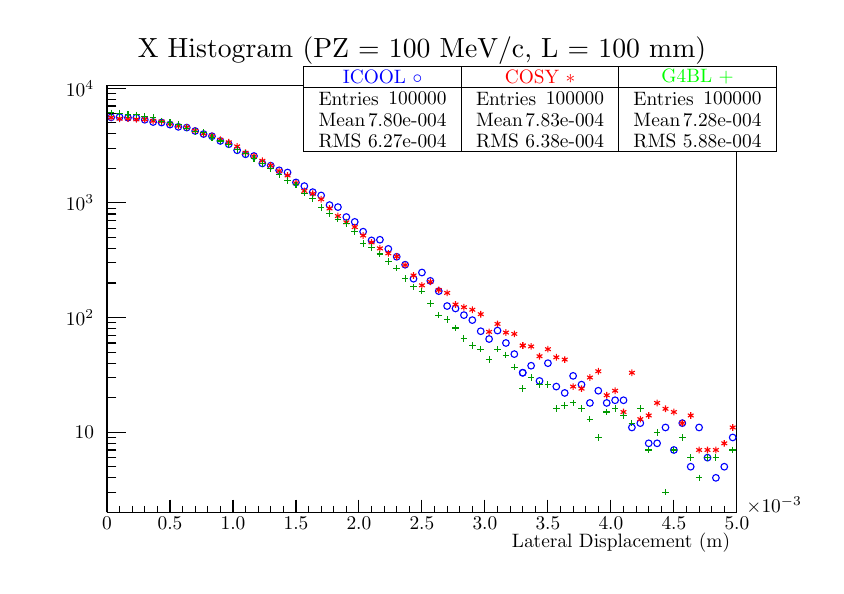
\begin{tikzpicture}
\definecolor{c}{rgb}{1,1,1};
\draw [color=c, fill=c] (0,0) rectangle (20,13.5632);
\draw [color=c, fill=c] (2,1.35632) rectangle (18,12.2069);
\definecolor{c}{rgb}{0,0,0};
\draw [c] (2,1.35632) -- (2,12.2069) -- (18,12.2069) -- (18,1.35632) -- (2,1.35632);
\definecolor{c}{rgb}{1,1,1};
\draw [color=c, fill=c] (2,1.35632) rectangle (18,12.2069);
\definecolor{c}{rgb}{0,0,0};
\draw [c] (2,1.35632) -- (2,12.2069) -- (18,12.2069) -- (18,1.35632) -- (2,1.35632);
\definecolor{c}{rgb}{0,0,1};
\foreach \P in
 {(2.10667,11.3888),(2.32,11.3986),(2.53333,11.3804),(2.74667,11.3806),(2.96,11.3281),(3.17333,11.2708),(3.38667,11.2568),(3.6,11.2053),(3.81333,11.1484),(4.02667,11.1299),(4.24,11.0434),(4.45333,10.9652),(4.66667,10.91),(4.88,10.7901),(5.09333,10.70
69),(5.30667,10.5534),(5.52,10.4509),(5.73333,10.4073),(5.94667,10.2193),(6.16,10.1625),(6.37333,10.0445),(6.58667,9.98877),(6.8,9.7364),(7.01333,9.64331),(7.22667,9.48993),(7.44,9.40564),(7.65333,9.16123),(7.86667,9.10998),(8.08,8.858),(8.29333,8.73
459),(8.50667,8.4857),(8.72,8.26453),(8.93333,8.28054),(9.14667,8.04834),(9.36,7.84857),(9.57333,7.64674),(9.78667,7.29014),(10,7.44811),(10.2133,7.23681),(10.4267,6.97558),(10.64,6.59674),(10.8533,6.53502),(11.0667,6.36613),(11.28,6.23954),(11.4933,
5.9573),(11.7067,5.75954),(11.92,5.97383),(12.1333,5.6583),(12.3467,5.37606),(12.56,4.90213)}{\draw[mark options={color=c,fill=c},mark size=2.402402pt,mark=o] plot coordinates {\P};}
\foreach \P in
 {(12.56,4.90213),(12.7733,5.08057),(12.9867,4.69431),(13.2,5.14545),(13.4133,4.55097),(13.6267,4.38928),(13.84,4.82305),(14.0533,4.60058),(14.2667,4.13547),(14.48,4.44551),(14.6933,4.13547),(14.9067,4.20385),(15.12,4.20385),(15.3333,3.51256),(15.546
7,3.62262),(15.76,3.10977),(15.9733,3.10977),(16.1867,3.51256),(16.4,2.94087),(16.6133,3.62262),(16.8267,2.51529),(17.04,3.51256),(17.2533,2.74589),(17.4667,2.23304),(17.68,2.51529),(17.8933,3.25874)}{\draw[mark options={color=c,fill=c},mark
 size=2.402402pt,mark=o] plot coordinates {\P};}
\definecolor{c}{rgb}{1,1,1};
\draw [color=c, fill=c] (7,10.5115) rectangle (11,12.6816);
\definecolor{c}{rgb}{0,0,0};
\draw [c] (7,10.5115) -- (11,10.5115);
\draw [c] (11,10.5115) -- (11,12.6816);
\draw [c] (11,12.6816) -- (7,12.6816);
\draw [c] (7,12.6816) -- (7,10.5115);
\draw[color=blue](9,12.4103) node[scale=0.7, rotate=0]{ICOOL $\circ$};
\draw [c] (7,12.1391) -- (11,12.1391);
\draw [anchor= west] (7.2,11.8678) node[scale=0.7, rotate=0]{Entries };
\draw [anchor= east] (10.8,11.8678) node[scale=0.7, rotate=0]{ 100000};
\draw [anchor= west] (7.2,11.3253) node[scale=0.7, rotate=0]{Mean  };
\draw [anchor= east] (10.8,11.3253) node[scale=0.7, rotate=0]{ 7.80e-004};
\draw [anchor= west] (7.2,10.7828) node[scale=0.7, rotate=0]{RMS   };
\draw [anchor= east] (10.8,10.7828) node[scale=0.7, rotate=0]{ 6.27e-004};
\draw [c] (2,1.35632) -- (18,1.35632);
\draw [anchor= east] (18,0.596782) node[scale=0.7, rotate=0]{Lateral Displacement (m)};
\draw [c] (2,1.68184) -- (2,1.35632);
\draw [c] (2.32,1.51908) -- (2.32,1.35632);
\draw [c] (2.64,1.51908) -- (2.64,1.35632);
\draw [c] (2.96,1.51908) -- (2.96,1.35632);
\draw [c] (3.28,1.51908) -- (3.28,1.35632);
\draw [c] (3.6,1.68184) -- (3.6,1.35632);
\draw [c] (3.92,1.51908) -- (3.92,1.35632);
\draw [c] (4.24,1.51908) -- (4.24,1.35632);
\draw [c] (4.56,1.51908) -- (4.56,1.35632);
\draw [c] (4.88,1.51908) -- (4.88,1.35632);
\draw [c] (5.2,1.68184) -- (5.2,1.35632);
\draw [c] (5.52,1.51908) -- (5.52,1.35632);
\draw [c] (5.84,1.51908) -- (5.84,1.35632);
\draw [c] (6.16,1.51908) -- (6.16,1.35632);
\draw [c] (6.48,1.51908) -- (6.48,1.35632);
\draw [c] (6.8,1.68184) -- (6.8,1.35632);
\draw [c] (7.12,1.51908) -- (7.12,1.35632);
\draw [c] (7.44,1.51908) -- (7.44,1.35632);
\draw [c] (7.76,1.51908) -- (7.76,1.35632);
\draw [c] (8.08,1.51908) -- (8.08,1.35632);
\draw [c] (8.4,1.68184) -- (8.4,1.35632);
\draw [c] (8.72,1.51908) -- (8.72,1.35632);
\draw [c] (9.04,1.51908) -- (9.04,1.35632);
\draw [c] (9.36,1.51908) -- (9.36,1.35632);
\draw [c] (9.68,1.51908) -- (9.68,1.35632);
\draw [c] (10,1.68184) -- (10,1.35632);
\draw [c] (10.32,1.51908) -- (10.32,1.35632);
\draw [c] (10.64,1.51908) -- (10.64,1.35632);
\draw [c] (10.96,1.51908) -- (10.96,1.35632);
\draw [c] (11.28,1.51908) -- (11.28,1.35632);
\draw [c] (11.6,1.68184) -- (11.6,1.35632);
\draw [c] (11.92,1.51908) -- (11.92,1.35632);
\draw [c] (12.24,1.51908) -- (12.24,1.35632);
\draw [c] (12.56,1.51908) -- (12.56,1.35632);
\draw [c] (12.88,1.51908) -- (12.88,1.35632);
\draw [c] (13.2,1.68184) -- (13.2,1.35632);
\draw [c] (13.52,1.51908) -- (13.52,1.35632);
\draw [c] (13.84,1.51908) -- (13.84,1.35632);
\draw [c] (14.16,1.51908) -- (14.16,1.35632);
\draw [c] (14.48,1.51908) -- (14.48,1.35632);
\draw [c] (14.8,1.68184) -- (14.8,1.35632);
\draw [c] (15.12,1.51908) -- (15.12,1.35632);
\draw [c] (15.44,1.51908) -- (15.44,1.35632);
\draw [c] (15.76,1.51908) -- (15.76,1.35632);
\draw [c] (16.08,1.51908) -- (16.08,1.35632);
\draw [c] (16.4,1.68184) -- (16.4,1.35632);
\draw [c] (16.72,1.51908) -- (16.72,1.35632);
\draw [c] (17.04,1.51908) -- (17.04,1.35632);
\draw [c] (17.36,1.51908) -- (17.36,1.35632);
\draw [c] (17.68,1.51908) -- (17.68,1.35632);
\draw [c] (18,1.68184) -- (18,1.35632);
\draw [c] (18,1.68184) -- (18,1.35632);
\draw [anchor=base] (2,0.908736) node[scale=0.7, rotate=0]{0};
\draw [anchor=base] (3.6,0.908736) node[scale=0.7, rotate=0]{0.5};
\draw [anchor=base] (5.2,0.908736) node[scale=0.7, rotate=0]{1.0};
\draw [anchor=base] (6.8,0.908736) node[scale=0.7, rotate=0]{1.5};
\draw [anchor=base] (8.4,0.908736) node[scale=0.7, rotate=0]{2.0};
\draw [anchor=base] (10,0.908736) node[scale=0.7, rotate=0]{2.5};
\draw [anchor=base] (11.6,0.908736) node[scale=0.7, rotate=0]{3.0};
\draw [anchor=base] (13.2,0.908736) node[scale=0.7, rotate=0]{3.5};
\draw [anchor=base] (14.8,0.908736) node[scale=0.7, rotate=0]{4.0};
\draw [anchor=base] (16.4,0.908736) node[scale=0.7, rotate=0]{4.5};
\draw [anchor=base] (18,0.908736) node[scale=0.7, rotate=0]{5.0};
\draw [anchor=base west] (18.07,1.35632) node[scale=0.7, rotate=0]{$\times10^{-3}$};
\draw [c] (2,1.35632) -- (2,12.2069);
\draw [c] (2.24,1.86917) -- (2,1.86917);
\draw [c] (2.24,2.23304) -- (2,2.23304);
\draw [c] (2.24,2.51528) -- (2,2.51528);
\draw [c] (2.24,2.74589) -- (2,2.74589);
\draw [c] (2.24,2.94087) -- (2,2.94087);
\draw [c] (2.24,3.10976) -- (2,3.10976);
\draw [c] (2.24,3.25874) -- (2,3.25874);
\draw [c] (2.48,3.39201) -- (2,3.39201);
\draw [anchor= east] (1.844,3.39201) node[scale=0.7, rotate=0]{10};
\draw [c] (2.24,4.26873) -- (2,4.26873);
\draw [c] (2.24,4.78158) -- (2,4.78158);
\draw [c] (2.24,5.14545) -- (2,5.14545);
\draw [c] (2.24,5.42769) -- (2,5.42769);
\draw [c] (2.24,5.6583) -- (2,5.6583);
\draw [c] (2.24,5.85328) -- (2,5.85328);
\draw [c] (2.24,6.02217) -- (2,6.02217);
\draw [c] (2.24,6.17115) -- (2,6.17115);
\draw [c] (2.48,6.30441) -- (2,6.30441);
\draw [anchor= east] (1.844,6.30441) node[scale=0.7, rotate=0]{$10^{2}$};
\draw [c] (2.24,7.18114) -- (2,7.18114);
\draw [c] (2.24,7.69399) -- (2,7.69399);
\draw [c] (2.24,8.05786) -- (2,8.05786);
\draw [c] (2.24,8.3401) -- (2,8.3401);
\draw [c] (2.24,8.57071) -- (2,8.57071);
\draw [c] (2.24,8.76569) -- (2,8.76569);
\draw [c] (2.24,8.93458) -- (2,8.93458);
\draw [c] (2.24,9.08356) -- (2,9.08356);
\draw [c] (2.48,9.21682) -- (2,9.21682);
\draw [anchor= east] (1.844,9.21682) node[scale=0.7, rotate=0]{$10^{3}$};
\draw [c] (2.24,10.0935) -- (2,10.0935);
\draw [c] (2.24,10.6064) -- (2,10.6064);
\draw [c] (2.24,10.9703) -- (2,10.9703);
\draw [c] (2.24,11.2525) -- (2,11.2525);
\draw [c] (2.24,11.4831) -- (2,11.4831);
\draw [c] (2.24,11.6781) -- (2,11.6781);
\draw [c] (2.24,11.847) -- (2,11.847);
\draw [c] (2.24,11.996) -- (2,11.996);
\draw [c] (2.48,12.1292) -- (2,12.1292);
\draw [anchor= east] (1.844,12.1292) node[scale=0.7, rotate=0]{$10^{4}$};
\definecolor{c}{rgb}{1,1,1};
\draw [color=c, fill=c] (7,10.5115) rectangle (11,12.6816);
\definecolor{c}{rgb}{0,0,0};
\draw [c] (7,10.5115) -- (11,10.5115);
\draw [c] (11,10.5115) -- (11,12.6816);
\draw [c] (11,12.6816) -- (7,12.6816);
\draw [c] (7,12.6816) -- (7,10.5115);
\draw[color=blue](9,12.4103) node[scale=0.7, rotate=0]{ICOOL $\circ$};
\draw [c] (7,12.1391) -- (11,12.1391);
\draw [anchor= west] (7.2,11.8678) node[scale=0.7, rotate=0]{Entries };
\draw [anchor= east] (10.8,11.8678) node[scale=0.7, rotate=0]{ 100000};
\draw [anchor= west] (7.2,11.3253) node[scale=0.7, rotate=0]{Mean  };
\draw [anchor= east] (10.8,11.3253) node[scale=0.7, rotate=0]{ 7.80e-004};
\draw [anchor= west] (7.2,10.7828) node[scale=0.7, rotate=0]{RMS   };
\draw [anchor= east] (10.8,10.7828) node[scale=0.7, rotate=0]{ 6.27e-004};
\draw (10,13.0816) node[scale=1, rotate=0]{X Histogram (PZ = 100 MeV/c, L = 100 mm)};
\definecolor{c}{rgb}{1,0,0};
\foreach \P in
 {(2.10667,11.3856),(2.32,11.3538),(2.53333,11.3601),(2.74667,11.3379),(2.96,11.339),(3.17333,11.2982),(3.38667,11.2857),(3.6,11.227),(3.81333,11.1718),(4.02667,11.1352),(4.24,11.0484),(4.45333,10.9741),(4.66667,10.9167),(4.88,10.8204),(5.09333,10.75
61),(5.30667,10.6519),(5.52,10.4913),(5.73333,10.4038),(5.94667,10.2873),(6.16,10.1661),(6.37333,10.0273),(6.58667,9.91376),(6.8,9.71866),(7.01333,9.52113),(7.22667,9.44743),(7.44,9.31065),(7.65333,9.0751),(7.86667,8.88295),(8.08,8.72343),(8.29333,8.
60194),(8.50667,8.38728),(8.72,8.21245),(8.93333,8.06102),(9.14667,7.93509),(9.36,7.85601),(9.57333,7.63796),(9.78667,7.37431),(10,7.1229),(10.2133,7.21237),(10.4267,7.00499),(10.64,6.93013),(10.8533,6.63627),(11.0667,6.56626),(11.28,6.503),(11.4933,
6.38999),(11.7067,5.94054),(11.92,6.14273),(12.1333,5.92357),(12.3467,5.88891),(12.56,5.59342)}{\draw[mark options={color=c,fill=c},mark size=2.402402pt,mark=asterisk] plot coordinates {\P};}
\foreach \P in
 {(12.56,5.59342),(12.7733,5.57104),(12.9867,5.32223),(13.2,5.50139),(13.4133,5.29443),(13.6267,5.23693),(13.84,4.55097),(14.0533,4.49934),(14.2667,4.78158),(14.48,4.93989),(14.6933,4.33044),(14.9067,4.44551),(15.12,3.90486),(15.3333,4.90213),(15.546
7,3.72386),(15.76,3.81759),(15.9733,4.13547),(16.1867,3.98649),(16.4,3.90486),(16.6133,3.62262),(16.8267,3.81759),(17.04,2.94087),(17.2533,2.94087),(17.4667,2.94087),(17.68,3.10977),(17.8933,3.51256)}{\draw[mark options={color=c,fill=c},mark
 size=2.402402pt,mark=asterisk] plot coordinates {\P};}
\definecolor{c}{rgb}{1,1,1};
\draw [color=c, fill=c] (11,10.5115) rectangle (15,12.6816);
\definecolor{c}{rgb}{0,0,0};
\draw [c] (11,10.5115) -- (15,10.5115);
\draw [c] (15,10.5115) -- (15,12.6816);
\draw [c] (15,12.6816) -- (11,12.6816);
\draw [c] (11,12.6816) -- (11,10.5115);
\draw [color=red](13,12.4103) node[scale=0.7, rotate=0]{COSY $*$};
\draw [c] (11,12.1391) -- (15,12.1391);
\draw [anchor= west] (11.2,11.8678) node[scale=0.7, rotate=0]{Entries };
\draw [anchor= east] (14.8,11.8678) node[scale=0.7, rotate=0]{ 100000};
\draw [anchor= west] (11.2,11.3253) node[scale=0.7, rotate=0]{Mean  };
\draw [anchor= east] (14.8,11.3253) node[scale=0.7, rotate=0]{ 7.83e-004};
\draw [anchor= west] (11.2,10.7828) node[scale=0.7, rotate=0]{RMS   };
\draw [anchor= east] (14.8,10.7828) node[scale=0.7, rotate=0]{ 6.38e-004};
\definecolor{c}{rgb}{1,1,1};
\draw [color=c, fill=c] (11,10.5115) rectangle (15,12.6816);
\definecolor{c}{rgb}{0,0,0};
\draw [c] (11,10.5115) -- (15,10.5115);
\draw [c] (15,10.5115) -- (15,12.6816);
\draw [c] (15,12.6816) -- (11,12.6816);
\draw [c] (11,12.6816) -- (11,10.5115);
\draw [color=red](13,12.4103) node[scale=0.7, rotate=0]{COSY $*$};
\draw [c] (11,12.1391) -- (15,12.1391);
\draw [anchor= west] (11.2,11.8678) node[scale=0.7, rotate=0]{Entries };
\draw [anchor= east] (14.8,11.8678) node[scale=0.7, rotate=0]{ 100000};
\draw [anchor= west] (11.2,11.3253) node[scale=0.7, rotate=0]{Mean  };
\draw [anchor= east] (14.8,11.3253) node[scale=0.7, rotate=0]{ 7.83e-004};
\draw [anchor= west] (11.2,10.7828) node[scale=0.7, rotate=0]{RMS   };
\draw [anchor= east] (14.8,10.7828) node[scale=0.7, rotate=0]{ 6.38e-004};
\definecolor{c}{rgb}{0,0.6,0};
\foreach \P in
 {(2.10667,11.5042),(2.32,11.4928),(2.53333,11.4541),(2.74667,11.4515),(2.96,11.4078),(3.17333,11.3868),(3.38667,11.2928),(3.6,11.2543),(3.81333,11.2145),(4.02667,11.1153),(4.24,11.0371),(4.45333,11.0018),(4.66667,10.8713),(4.88,10.7883),(5.09333,10.
7072),(5.30667,10.5796),(5.52,10.4713),(5.73333,10.3523),(5.94667,10.2152),(6.16,10.0942),(6.37333,9.94188),(6.58667,9.78009),(6.8,9.67364),(7.01333,9.46523),(7.22667,9.32699),(7.44,9.10585),(7.65333,8.93932),(7.86667,8.80483),(8.08,8.70081),(8.29333
,8.48345),(8.50667,8.18415),(8.72,8.07669),(8.93333,7.91755),(9.14667,7.73546),(9.36,7.56072),(9.57333,7.29014),(9.78667,7.08253),(10,6.97558),(10.2133,6.65558),(10.4267,6.36613),(10.64,6.25278),(10.8533,6.03789),(11.0667,5.77885),(11.28,5.59342),(11
.4933,5.50139),(11.7067,5.23693),(11.92,5.50139),(12.1333,5.34943),(12.3467,5.04684),(12.56,4.49934)}{\draw[mark options={color=c,fill=c},mark size=2.402402pt,mark=+] plot coordinates {\P};}
\foreach \P in
 {(12.56,4.49934),(12.7733,4.78158),(12.9867,4.60058),(13.2,4.60058),(13.4133,3.98649),(13.6267,4.06317),(13.84,4.13547),(14.0533,3.98649),(14.2667,3.72386),(14.48,3.25874),(14.6933,3.90486),(14.9067,3.98649),(15.12,3.81759),(15.3333,3.62262),(15.546
7,3.98649),(15.76,2.94087),(15.9733,3.39201),(16.1867,1.86917),(16.4,2.94087),(16.6133,3.25874),(16.8267,2.74589),(17.04,2.23304),(17.2533,2.74589),(17.4667,2.74589),(17.8933,2.94087)}{\draw[mark options={color=c,fill=c},mark size=2.402402pt,mark=+]
 plot coordinates {\P};}
\definecolor{c}{rgb}{1,1,1};
\draw [color=c, fill=c] (15,10.5115) rectangle (19,12.6816);
\definecolor{c}{rgb}{0,0,0};
\draw [c] (15,10.5115) -- (19,10.5115);
\draw [c] (19,10.5115) -- (19,12.6816);
\draw [c] (19,12.6816) -- (15,12.6816);
\draw [c] (15,12.6816) -- (15,10.5115);
\draw [color=green](17,12.4103) node[scale=0.7, rotate=0]{G4BL $+$};
\draw [c] (15,12.1391) -- (19,12.1391);
\draw [anchor= west] (15.2,11.8678) node[scale=0.7, rotate=0]{Entries };
\draw [anchor= east] (18.8,11.8678) node[scale=0.7, rotate=0]{ 100000};
\draw [anchor= west] (15.2,11.3253) node[scale=0.7, rotate=0]{Mean  };
\draw [anchor= east] (18.8,11.3253) node[scale=0.7, rotate=0]{ 7.28e-004};
\draw [anchor= west] (15.2,10.7828) node[scale=0.7, rotate=0]{RMS   };
\draw [anchor= east] (18.8,10.7828) node[scale=0.7, rotate=0]{ 5.88e-004};
\definecolor{c}{rgb}{1,1,1};
\draw [color=c, fill=c] (15,10.5115) rectangle (19,12.6816);
\definecolor{c}{rgb}{0,0,0};
\draw [c] (15,10.5115) -- (19,10.5115);
\draw [c] (19,10.5115) -- (19,12.6816);
\draw [c] (19,12.6816) -- (15,12.6816);
\draw [c] (15,12.6816) -- (15,10.5115);
\draw [color=green](17,12.4103) node[scale=0.7, rotate=0]{G4BL $+$};
\draw [c] (15,12.1391) -- (19,12.1391);
\draw [anchor= west] (15.2,11.8678) node[scale=0.7, rotate=0]{Entries };
\draw [anchor= east] (18.8,11.8678) node[scale=0.7, rotate=0]{ 100000};
\draw [anchor= west] (15.2,11.3253) node[scale=0.7, rotate=0]{Mean  };
\draw [anchor= east] (18.8,11.3253) node[scale=0.7, rotate=0]{ 7.28e-004};
\draw [anchor= west] (15.2,10.7828) node[scale=0.7, rotate=0]{RMS   };
\draw [anchor= east] (18.8,10.7828) node[scale=0.7, rotate=0]{ 5.88e-004};
\end{tikzpicture}
}\\
\frame{    \pgfdeclareplotmark{cross} {
\pgfpathmoveto{\pgfpoint{-0.3\pgfplotmarksize}{\pgfplotmarksize}}
\pgfpathlineto{\pgfpoint{+0.3\pgfplotmarksize}{\pgfplotmarksize}}
\pgfpathlineto{\pgfpoint{+0.3\pgfplotmarksize}{0.3\pgfplotmarksize}}
\pgfpathlineto{\pgfpoint{+1\pgfplotmarksize}{0.3\pgfplotmarksize}}
\pgfpathlineto{\pgfpoint{+1\pgfplotmarksize}{-0.3\pgfplotmarksize}}
\pgfpathlineto{\pgfpoint{+0.3\pgfplotmarksize}{-0.3\pgfplotmarksize}}
\pgfpathlineto{\pgfpoint{+0.3\pgfplotmarksize}{-1.\pgfplotmarksize}}
\pgfpathlineto{\pgfpoint{-0.3\pgfplotmarksize}{-1.\pgfplotmarksize}}
\pgfpathlineto{\pgfpoint{-0.3\pgfplotmarksize}{-0.3\pgfplotmarksize}}
\pgfpathlineto{\pgfpoint{-1.\pgfplotmarksize}{-0.3\pgfplotmarksize}}
\pgfpathlineto{\pgfpoint{-1.\pgfplotmarksize}{0.3\pgfplotmarksize}}
\pgfpathlineto{\pgfpoint{-0.3\pgfplotmarksize}{0.3\pgfplotmarksize}}
\pgfpathclose
\pgfusepathqstroke
}
\pgfdeclareplotmark{cross*} {
\pgfpathmoveto{\pgfpoint{-0.3\pgfplotmarksize}{\pgfplotmarksize}}
\pgfpathlineto{\pgfpoint{+0.3\pgfplotmarksize}{\pgfplotmarksize}}
\pgfpathlineto{\pgfpoint{+0.3\pgfplotmarksize}{0.3\pgfplotmarksize}}
\pgfpathlineto{\pgfpoint{+1\pgfplotmarksize}{0.3\pgfplotmarksize}}
\pgfpathlineto{\pgfpoint{+1\pgfplotmarksize}{-0.3\pgfplotmarksize}}
\pgfpathlineto{\pgfpoint{+0.3\pgfplotmarksize}{-0.3\pgfplotmarksize}}
\pgfpathlineto{\pgfpoint{+0.3\pgfplotmarksize}{-1.\pgfplotmarksize}}
\pgfpathlineto{\pgfpoint{-0.3\pgfplotmarksize}{-1.\pgfplotmarksize}}
\pgfpathlineto{\pgfpoint{-0.3\pgfplotmarksize}{-0.3\pgfplotmarksize}}
\pgfpathlineto{\pgfpoint{-1.\pgfplotmarksize}{-0.3\pgfplotmarksize}}
\pgfpathlineto{\pgfpoint{-1.\pgfplotmarksize}{0.3\pgfplotmarksize}}
\pgfpathlineto{\pgfpoint{-0.3\pgfplotmarksize}{0.3\pgfplotmarksize}}
\pgfpathclose
\pgfusepathqfillstroke
}
\pgfdeclareplotmark{newstar} {
\pgfpathmoveto{\pgfqpoint{0pt}{\pgfplotmarksize}}
\pgfpathlineto{\pgfqpointpolar{44}{0.5\pgfplotmarksize}}
\pgfpathlineto{\pgfqpointpolar{18}{\pgfplotmarksize}}
\pgfpathlineto{\pgfqpointpolar{-20}{0.5\pgfplotmarksize}}
\pgfpathlineto{\pgfqpointpolar{-54}{\pgfplotmarksize}}
\pgfpathlineto{\pgfqpointpolar{-90}{0.5\pgfplotmarksize}}
\pgfpathlineto{\pgfqpointpolar{234}{\pgfplotmarksize}}
\pgfpathlineto{\pgfqpointpolar{198}{0.5\pgfplotmarksize}}
\pgfpathlineto{\pgfqpointpolar{162}{\pgfplotmarksize}}
\pgfpathlineto{\pgfqpointpolar{134}{0.5\pgfplotmarksize}}
\pgfpathclose
\pgfusepathqstroke
}
\pgfdeclareplotmark{newstar*} {
\pgfpathmoveto{\pgfqpoint{0pt}{\pgfplotmarksize}}
\pgfpathlineto{\pgfqpointpolar{44}{0.5\pgfplotmarksize}}
\pgfpathlineto{\pgfqpointpolar{18}{\pgfplotmarksize}}
\pgfpathlineto{\pgfqpointpolar{-20}{0.5\pgfplotmarksize}}
\pgfpathlineto{\pgfqpointpolar{-54}{\pgfplotmarksize}}
\pgfpathlineto{\pgfqpointpolar{-90}{0.5\pgfplotmarksize}}
\pgfpathlineto{\pgfqpointpolar{234}{\pgfplotmarksize}}
\pgfpathlineto{\pgfqpointpolar{198}{0.5\pgfplotmarksize}}
\pgfpathlineto{\pgfqpointpolar{162}{\pgfplotmarksize}}
\pgfpathlineto{\pgfqpointpolar{134}{0.5\pgfplotmarksize}}
\pgfpathclose
\pgfusepathqfillstroke
}
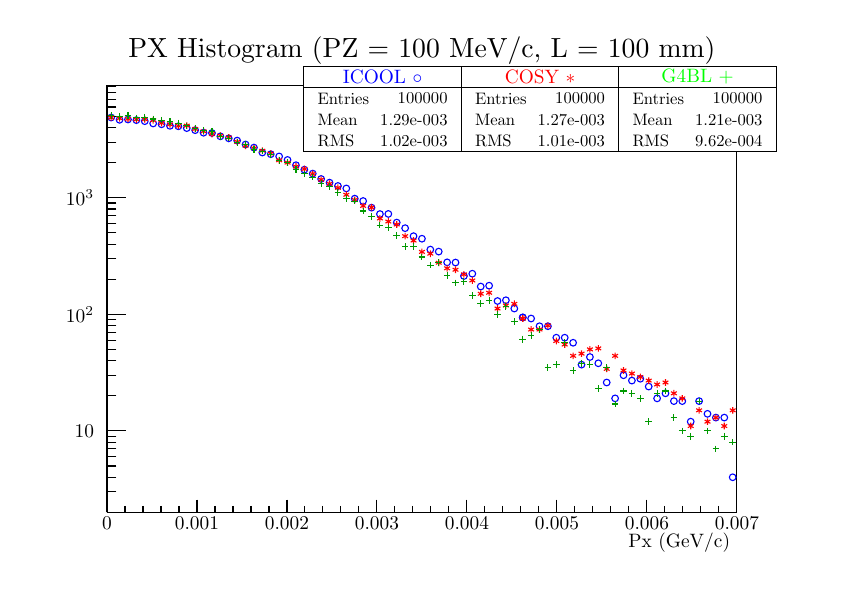
\begin{tikzpicture}
\definecolor{c}{rgb}{1,1,1};
\draw [color=c, fill=c] (0,0) rectangle (20,13.5632);
\draw [color=c, fill=c] (2,1.35632) rectangle (18,12.2069);
\definecolor{c}{rgb}{0,0,0};
\draw [c] (2,1.35632) -- (2,12.2069) -- (18,12.2069) -- (18,1.35632) -- (2,1.35632);
\definecolor{c}{rgb}{1,1,1};
\draw [color=c, fill=c] (2,1.35632) rectangle (18,12.2069);
\definecolor{c}{rgb}{0,0,0};
\draw [c] (2,1.35632) -- (2,12.2069) -- (18,12.2069) -- (18,1.35632) -- (2,1.35632);
\definecolor{c}{rgb}{0,0,1};
\foreach \P in
 {(2.10667,11.3851),(2.32,11.3265),(2.53333,11.3356),(2.74667,11.3185),(2.96,11.2921),(3.17333,11.2343),(3.38667,11.2128),(3.6,11.1742),(3.81333,11.1617),(4.02667,11.116),(4.24,11.0633),(4.45333,10.999),(4.66667,10.9918),(4.88,10.9071),(5.09333,10.85
64),(5.30667,10.7994),(5.52,10.7004),(5.73333,10.6217),(5.94667,10.4963),(6.16,10.4535),(6.37333,10.3967),(6.58667,10.3078),(6.8,10.1743),(7.01333,10.0605),(7.22667,9.9614),(7.44,9.82422),(7.65333,9.73124),(7.86667,9.6464),(8.08,9.58371),(8.29333,9.3
2481),(8.50667,9.26449),(8.72,9.0961),(8.93333,8.93285),(9.14667,8.9364),(9.36,8.71673),(9.57333,8.57468),(9.78667,8.37175),(10,8.30694),(10.2133,8.03077),(10.4267,7.97962),(10.64,7.70657),(10.8533,7.70195),(11.0667,7.35946),(11.28,7.41846),(11.4933,
7.09197),(11.7067,7.11408),(11.92,6.72449),(12.1333,6.74413),(12.3467,6.53284),(12.56,6.30753)}{\draw[mark options={color=c,fill=c},mark size=2.402402pt,mark=o] plot coordinates {\P};}
\foreach \P in
 {(12.56,6.30753),(12.7733,6.27987),(12.9867,6.08396),(13.2,6.08396),(13.4133,5.79293),(13.6267,5.79293),(13.84,5.66423),(14.0533,5.10851),(14.2667,5.30177),(14.48,5.14281),(14.6933,4.65479),(14.9067,4.25143),(15.12,4.83882),(15.3333,4.70332),(15.546
7,4.75009),(15.76,4.55186),(15.9733,4.25143),(16.1867,4.38014),(16.4,4.1819),(16.6133,4.1819),(16.8267,3.66049),(17.04,4.1819),(17.2533,3.85872),(17.4667,3.76342),(17.68,3.76342),(17.8933,2.24769)}{\draw[mark options={color=c,fill=c},mark
 size=2.402402pt,mark=o] plot coordinates {\P};}
\definecolor{c}{rgb}{1,1,1};
\draw [color=c, fill=c] (7,10.5115) rectangle (11,12.6816);
\definecolor{c}{rgb}{0,0,0};
\draw [c] (7,10.5115) -- (11,10.5115);
\draw [c] (11,10.5115) -- (11,12.6816);
\draw [c] (11,12.6816) -- (7,12.6816);
\draw [c] (7,12.6816) -- (7,10.5115);
\draw[color=blue](9,12.4103) node[scale=0.7, rotate=0]{ICOOL $\circ$};
\draw [c] (7,12.1391) -- (11,12.1391);
\draw [anchor= west] (7.2,11.8678) node[scale=0.6, rotate=0]{Entries };
\draw [anchor= east] (10.8,11.8678) node[scale=0.6, rotate=0]{ 100000};
\draw [anchor= west] (7.2,11.3253) node[scale=0.6, rotate=0]{Mean  };
\draw [anchor= east] (10.8,11.3253) node[scale=0.6, rotate=0]{ 1.29e-003};
\draw [anchor= west] (7.2,10.7828) node[scale=0.6, rotate=0]{RMS   };
\draw [anchor= east] (10.8,10.7828) node[scale=0.6, rotate=0]{ 1.02e-003};
\draw [c] (2,1.35632) -- (18,1.35632);
\draw [anchor= east] (18,0.596782) node[scale=0.7, rotate=0]{Px (GeV/c)};
\draw [c] (2,1.68184) -- (2,1.35632);
\draw [c] (2.45714,1.51908) -- (2.45714,1.35632);
\draw [c] (2.91429,1.51908) -- (2.91429,1.35632);
\draw [c] (3.37143,1.51908) -- (3.37143,1.35632);
\draw [c] (3.82857,1.51908) -- (3.82857,1.35632);
\draw [c] (4.28571,1.68184) -- (4.28571,1.35632);
\draw [c] (4.74286,1.51908) -- (4.74286,1.35632);
\draw [c] (5.2,1.51908) -- (5.2,1.35632);
\draw [c] (5.65714,1.51908) -- (5.65714,1.35632);
\draw [c] (6.11429,1.51908) -- (6.11429,1.35632);
\draw [c] (6.57143,1.68184) -- (6.57143,1.35632);
\draw [c] (7.02857,1.51908) -- (7.02857,1.35632);
\draw [c] (7.48571,1.51908) -- (7.48571,1.35632);
\draw [c] (7.94286,1.51908) -- (7.94286,1.35632);
\draw [c] (8.4,1.51908) -- (8.4,1.35632);
\draw [c] (8.85714,1.68184) -- (8.85714,1.35632);
\draw [c] (9.31429,1.51908) -- (9.31429,1.35632);
\draw [c] (9.77143,1.51908) -- (9.77143,1.35632);
\draw [c] (10.2286,1.51908) -- (10.2286,1.35632);
\draw [c] (10.6857,1.51908) -- (10.6857,1.35632);
\draw [c] (11.1429,1.68184) -- (11.1429,1.35632);
\draw [c] (11.6,1.51908) -- (11.6,1.35632);
\draw [c] (12.0571,1.51908) -- (12.0571,1.35632);
\draw [c] (12.5143,1.51908) -- (12.5143,1.35632);
\draw [c] (12.9714,1.51908) -- (12.9714,1.35632);
\draw [c] (13.4286,1.68184) -- (13.4286,1.35632);
\draw [c] (13.8857,1.51908) -- (13.8857,1.35632);
\draw [c] (14.3429,1.51908) -- (14.3429,1.35632);
\draw [c] (14.8,1.51908) -- (14.8,1.35632);
\draw [c] (15.2571,1.51908) -- (15.2571,1.35632);
\draw [c] (15.7143,1.68184) -- (15.7143,1.35632);
\draw [c] (16.1714,1.51908) -- (16.1714,1.35632);
\draw [c] (16.6286,1.51908) -- (16.6286,1.35632);
\draw [c] (17.0857,1.51908) -- (17.0857,1.35632);
\draw [c] (17.5429,1.51908) -- (17.5429,1.35632);
\draw [c] (18,1.68184) -- (18,1.35632);
\draw [c] (18,1.68184) -- (18,1.35632);
\draw [anchor=base] (2,0.908736) node[scale=0.7, rotate=0]{0};
\draw [anchor=base] (4.28571,0.908736) node[scale=0.7, rotate=0]{0.001};
\draw [anchor=base] (6.57143,0.908736) node[scale=0.7, rotate=0]{0.002};
\draw [anchor=base] (8.85714,0.908736) node[scale=0.7, rotate=0]{0.003};
\draw [anchor=base] (11.1429,0.908736) node[scale=0.7, rotate=0]{0.004};
\draw [anchor=base] (13.4286,0.908736) node[scale=0.7, rotate=0]{0.005};
\draw [anchor=base] (15.7143,0.908736) node[scale=0.7, rotate=0]{0.006};
\draw [anchor=base] (18,0.908736) node[scale=0.7, rotate=0]{0.007};
\draw [c] (2,1.35632) -- (2,12.2069);
\draw [c] (2.24,1.87774) -- (2,1.87774);
\draw [c] (2.24,2.24769) -- (2,2.24769);
\draw [c] (2.24,2.53465) -- (2,2.53465);
\draw [c] (2.24,2.76911) -- (2,2.76911);
\draw [c] (2.24,2.96735) -- (2,2.96735);
\draw [c] (2.24,3.13906) -- (2,3.13906);
\draw [c] (2.24,3.29053) -- (2,3.29053);
\draw [c] (2.48,3.42602) -- (2,3.42602);
\draw [anchor= east] (1.844,3.42602) node[scale=0.7, rotate=0]{10};
\draw [c] (2.24,4.31739) -- (2,4.31739);
\draw [c] (2.24,4.83881) -- (2,4.83881);
\draw [c] (2.24,5.20877) -- (2,5.20877);
\draw [c] (2.24,5.49572) -- (2,5.49572);
\draw [c] (2.24,5.73019) -- (2,5.73019);
\draw [c] (2.24,5.92842) -- (2,5.92842);
\draw [c] (2.24,6.10014) -- (2,6.10014);
\draw [c] (2.24,6.25161) -- (2,6.25161);
\draw [c] (2.48,6.3871) -- (2,6.3871);
\draw [anchor= east] (1.844,6.3871) node[scale=0.7, rotate=0]{$10^{2}$};
\draw [c] (2.24,7.27847) -- (2,7.27847);
\draw [c] (2.24,7.79989) -- (2,7.79989);
\draw [c] (2.24,8.16984) -- (2,8.16984);
\draw [c] (2.24,8.4568) -- (2,8.4568);
\draw [c] (2.24,8.69126) -- (2,8.69126);
\draw [c] (2.24,8.8895) -- (2,8.8895);
\draw [c] (2.24,9.06121) -- (2,9.06121);
\draw [c] (2.24,9.21268) -- (2,9.21268);
\draw [c] (2.48,9.34817) -- (2,9.34817);
\draw [anchor= east] (1.844,9.34817) node[scale=0.7, rotate=0]{$10^{3}$};
\draw [c] (2.24,10.2395) -- (2,10.2395);
\draw [c] (2.24,10.761) -- (2,10.761);
\draw [c] (2.24,11.1309) -- (2,11.1309);
\draw [c] (2.24,11.4179) -- (2,11.4179);
\draw [c] (2.24,11.6523) -- (2,11.6523);
\draw [c] (2.24,11.8506) -- (2,11.8506);
\draw [c] (2.24,12.0223) -- (2,12.0223);
\draw [c] (2.24,12.1738) -- (2,12.1738);
\definecolor{c}{rgb}{1,1,1};
\draw [color=c, fill=c] (7,10.5115) rectangle (11,12.6816);
\definecolor{c}{rgb}{0,0,0};
\draw [c] (7,10.5115) -- (11,10.5115);
\draw [c] (11,10.5115) -- (11,12.6816);
\draw [c] (11,12.6816) -- (7,12.6816);
\draw [c] (7,12.6816) -- (7,10.5115);
\draw[color=blue](9,12.4103) node[scale=0.7, rotate=0]{ICOOL $\circ$};
\draw [c] (7,12.1391) -- (11,12.1391);
\draw [anchor= west] (7.2,11.8678) node[scale=0.6, rotate=0]{Entries };
\draw [anchor= east] (10.8,11.8678) node[scale=0.6, rotate=0]{ 100000};
\draw [anchor= west] (7.2,11.3253) node[scale=0.6, rotate=0]{Mean  };
\draw [anchor= east] (10.8,11.3253) node[scale=0.6, rotate=0]{ 1.29e-003};
\draw [anchor= west] (7.2,10.7828) node[scale=0.6, rotate=0]{RMS   };
\draw [anchor= east] (10.8,10.7828) node[scale=0.6, rotate=0]{ 1.02e-003};
\draw (10,13.0816) node[scale=1, rotate=0]{PX Histogram (PZ = 100 MeV/c, L = 100 mm)};
\definecolor{c}{rgb}{1,0,0};
\foreach \P in
 {(2.10667,11.3821),(2.32,11.3646),(2.53333,11.35),(2.74667,11.3345),(2.96,11.3402),(3.17333,11.3171),(3.38667,11.2456),(3.6,11.2107),(3.81333,11.173),(4.02667,11.1789),(4.24,11.0937),(4.45333,11.0345),(4.66667,10.9662),(4.88,10.9242),(5.09333,10.879
2),(5.30667,10.7674),(5.52,10.6695),(5.73333,10.6034),(5.94667,10.5424),(6.16,10.4692),(6.37333,10.2992),(6.58667,10.2395),(6.8,10.1393),(7.01333,10.0781),(7.22667,9.95259),(7.44,9.80723),(7.65333,9.7013),(7.86667,9.59967),(8.08,9.42311),(8.29333,9.2
9165),(8.50667,9.14069),(8.72,9.10234),(8.93333,8.8216),(9.14667,8.74376),(9.36,8.66747),(9.57333,8.37175),(9.78667,8.25985),(10,7.97214),(10.2133,7.92635),(10.4267,7.69731),(10.64,7.5551),(10.8533,7.51828),(11.0667,7.40104),(11.28,7.24591),(11.4933,
6.90852),(11.7067,6.93398),(11.92,6.53284),(12.1333,6.6108),(12.3467,6.65331),(12.56,6.27987)}{\draw[mark options={color=c,fill=c},mark size=2.402402pt,mark=asterisk] plot coordinates {\P};}
\foreach \P in
 {(12.56,6.27987),(12.7733,5.99988),(12.9867,5.99988),(13.2,6.10014),(13.4133,5.70857),(13.6267,5.61829),(13.84,5.33134),(14.0533,5.3885),(14.2667,5.49573),(14.48,5.52119),(14.6933,4.99977),(14.9067,5.33134),(15.12,4.96138),(15.3333,4.88098),(15.5467
,4.79522),(15.76,4.70332),(15.9733,4.60435),(16.1867,4.65479),(16.4,4.38014),(16.6133,4.25143),(16.8267,3.54859),(17.04,3.94744),(17.2533,3.66049),(17.4667,3.76342),(17.68,3.54859),(17.8933,3.94744)}{\draw[mark options={color=c,fill=c},mark
 size=2.402402pt,mark=asterisk] plot coordinates {\P};}
\definecolor{c}{rgb}{1,1,1};
\draw [color=c, fill=c] (11,10.5115) rectangle (15,12.6816);
\definecolor{c}{rgb}{0,0,0};
\draw [c] (11,10.5115) -- (15,10.5115);
\draw [c] (15,10.5115) -- (15,12.6816);
\draw [c] (15,12.6816) -- (11,12.6816);
\draw [c] (11,12.6816) -- (11,10.5115);
\draw [color=red](13,12.4103) node[scale=0.7, rotate=0]{COSY $*$};
\draw [c] (11,12.1391) -- (15,12.1391);
\draw [anchor= west] (11.2,11.8678) node[scale=0.6, rotate=0]{Entries };
\draw [anchor= east] (14.8,11.8678) node[scale=0.6, rotate=0]{ 100000};
\draw [anchor= west] (11.2,11.3253) node[scale=0.6, rotate=0]{Mean  };
\draw [anchor= east] (14.8,11.3253) node[scale=0.6, rotate=0]{ 1.27e-003};
\draw [anchor= west] (11.2,10.7828) node[scale=0.6, rotate=0]{RMS   };
\draw [anchor= east] (14.8,10.7828) node[scale=0.6, rotate=0]{ 1.01e-003};
\definecolor{c}{rgb}{1,1,1};
\draw [color=c, fill=c] (11,10.5115) rectangle (15,12.6816);
\definecolor{c}{rgb}{0,0,0};
\draw [c] (11,10.5115) -- (15,10.5115);
\draw [c] (15,10.5115) -- (15,12.6816);
\draw [c] (15,12.6816) -- (11,12.6816);
\draw [c] (11,12.6816) -- (11,10.5115);
\draw [color=red](13,12.4103) node[scale=0.7, rotate=0]{COSY $*$};
\draw [c] (11,12.1391) -- (15,12.1391);
\draw [anchor= west] (11.2,11.8678) node[scale=0.6, rotate=0]{Entries };
\draw [anchor= east] (14.8,11.8678) node[scale=0.6, rotate=0]{ 100000};
\draw [anchor= west] (11.2,11.3253) node[scale=0.6, rotate=0]{Mean  };
\draw [anchor= east] (14.8,11.3253) node[scale=0.6, rotate=0]{ 1.27e-003};
\draw [anchor= west] (11.2,10.7828) node[scale=0.6, rotate=0]{RMS   };
\draw [anchor= east] (14.8,10.7828) node[scale=0.6, rotate=0]{ 1.01e-003};
\definecolor{c}{rgb}{0,0.6,0};
\foreach \P in
 {(2.10667,11.4304),(2.32,11.4078),(2.53333,11.4289),(2.74667,11.3761),(2.96,11.3911),(3.17333,11.3487),(3.38667,11.3193),(3.6,11.2847),(3.81333,11.2417),(4.02667,11.1739),(4.24,11.1134),(4.45333,11.0605),(4.66667,11.0366),(4.88,10.9098),(5.09333,10.
8631),(5.30667,10.7571),(5.52,10.7062),(5.73333,10.5685),(5.94667,10.5316),(6.16,10.4381),(6.37333,10.2925),(6.58667,10.235),(6.8,10.0568),(7.01333,9.955),(7.22667,9.87045),(7.44,9.71297),(7.65333,9.63719),(7.86667,9.4789),(8.08,9.3235),(8.29333,9.26
312),(8.50667,9.01206),(8.72,8.86352),(8.93333,8.65209),(9.14667,8.5817),(9.36,8.39624),(9.57333,8.11063),(9.78667,8.11399),(10,7.84206),(10.2133,7.6355),(10.4267,7.70195),(10.64,7.36548),(10.8533,7.18515),(11.0667,7.22597),(11.28,6.86492),(11.4933,6
.65331),(11.7067,6.74413),(11.92,6.37417),(12.1333,6.57796),(12.3467,6.20801),(12.56,5.75144)}{\draw[mark options={color=c,fill=c},mark size=2.402402pt,mark=+] plot coordinates {\P};}
\foreach \P in
 {(12.56,5.75144),(12.7733,5.85275),(12.9867,5.99988),(13.2,5.03705),(13.4133,5.10851),(13.6267,5.66423),(13.84,4.96138),(14.0533,5.14281),(14.2667,5.10851),(14.48,4.49713),(14.6933,5.03705),(14.9067,4.1084),(15.12,4.43996),(15.3333,4.38014),(15.5467
,4.25143),(15.76,3.66049),(15.9733,4.38014),(16.1867,4.43996),(16.4,3.76342),(16.6133,3.42602),(16.8267,3.29053),(17.04,4.1819),(17.2533,3.42602),(17.4667,2.96735),(17.68,3.29053),(17.8933,3.13907)}{\draw[mark options={color=c,fill=c},mark
 size=2.402402pt,mark=+] plot coordinates {\P};}
\definecolor{c}{rgb}{1,1,1};
\draw [color=c, fill=c] (15,10.5115) rectangle (19,12.6816);
\definecolor{c}{rgb}{0,0,0};
\draw [c] (15,10.5115) -- (19,10.5115);
\draw [c] (19,10.5115) -- (19,12.6816);
\draw [c] (19,12.6816) -- (15,12.6816);
\draw [c] (15,12.6816) -- (15,10.5115);
\draw [color=green](17,12.4103) node[scale=0.7, rotate=0]{G4BL $+$};
\draw [c] (15,12.1391) -- (19,12.1391);
\draw [anchor= west] (15.2,11.8678) node[scale=0.6, rotate=0]{Entries };
\draw [anchor= east] (18.8,11.8678) node[scale=0.6, rotate=0]{ 100000};
\draw [anchor= west] (15.2,11.3253) node[scale=0.6, rotate=0]{Mean  };
\draw [anchor= east] (18.8,11.3253) node[scale=0.6, rotate=0]{ 1.21e-003};
\draw [anchor= west] (15.2,10.7828) node[scale=0.6, rotate=0]{RMS   };
\draw [anchor= east] (18.8,10.7828) node[scale=0.6, rotate=0]{ 9.62e-004};
\definecolor{c}{rgb}{1,1,1};
\draw [color=c, fill=c] (15,10.5115) rectangle (19,12.6816);
\definecolor{c}{rgb}{0,0,0};
\draw [c] (15,10.5115) -- (19,10.5115);
\draw [c] (19,10.5115) -- (19,12.6816);
\draw [c] (19,12.6816) -- (15,12.6816);
\draw [c] (15,12.6816) -- (15,10.5115);
\draw [color=green](17,12.4103) node[scale=0.7, rotate=0]{G4BL $+$};
\draw [c] (15,12.1391) -- (19,12.1391);
\draw [anchor= west] (15.2,11.8678) node[scale=0.6, rotate=0]{Entries };
\draw [anchor= east] (18.8,11.8678) node[scale=0.6, rotate=0]{ 100000};
\draw [anchor= west] (15.2,11.3253) node[scale=0.6, rotate=0]{Mean  };
\draw [anchor= east] (18.8,11.3253) node[scale=0.6, rotate=0]{ 1.21e-003};
\draw [anchor= west] (15.2,10.7828) node[scale=0.6, rotate=0]{RMS   };
\draw [anchor= east] (18.8,10.7828) node[scale=0.6, rotate=0]{ 9.62e-004};
\end{tikzpicture}
}\\
\frame{\pgfdeclareplotmark{cross} {
\pgfpathmoveto{\pgfpoint{-0.3\pgfplotmarksize}{\pgfplotmarksize}}
\pgfpathlineto{\pgfpoint{+0.3\pgfplotmarksize}{\pgfplotmarksize}}
\pgfpathlineto{\pgfpoint{+0.3\pgfplotmarksize}{0.3\pgfplotmarksize}}
\pgfpathlineto{\pgfpoint{+1\pgfplotmarksize}{0.3\pgfplotmarksize}}
\pgfpathlineto{\pgfpoint{+1\pgfplotmarksize}{-0.3\pgfplotmarksize}}
\pgfpathlineto{\pgfpoint{+0.3\pgfplotmarksize}{-0.3\pgfplotmarksize}}
\pgfpathlineto{\pgfpoint{+0.3\pgfplotmarksize}{-1.\pgfplotmarksize}}
\pgfpathlineto{\pgfpoint{-0.3\pgfplotmarksize}{-1.\pgfplotmarksize}}
\pgfpathlineto{\pgfpoint{-0.3\pgfplotmarksize}{-0.3\pgfplotmarksize}}
\pgfpathlineto{\pgfpoint{-1.\pgfplotmarksize}{-0.3\pgfplotmarksize}}
\pgfpathlineto{\pgfpoint{-1.\pgfplotmarksize}{0.3\pgfplotmarksize}}
\pgfpathlineto{\pgfpoint{-0.3\pgfplotmarksize}{0.3\pgfplotmarksize}}
\pgfpathclose
\pgfusepathqstroke
}
\pgfdeclareplotmark{cross*} {
\pgfpathmoveto{\pgfpoint{-0.3\pgfplotmarksize}{\pgfplotmarksize}}
\pgfpathlineto{\pgfpoint{+0.3\pgfplotmarksize}{\pgfplotmarksize}}
\pgfpathlineto{\pgfpoint{+0.3\pgfplotmarksize}{0.3\pgfplotmarksize}}
\pgfpathlineto{\pgfpoint{+1\pgfplotmarksize}{0.3\pgfplotmarksize}}
\pgfpathlineto{\pgfpoint{+1\pgfplotmarksize}{-0.3\pgfplotmarksize}}
\pgfpathlineto{\pgfpoint{+0.3\pgfplotmarksize}{-0.3\pgfplotmarksize}}
\pgfpathlineto{\pgfpoint{+0.3\pgfplotmarksize}{-1.\pgfplotmarksize}}
\pgfpathlineto{\pgfpoint{-0.3\pgfplotmarksize}{-1.\pgfplotmarksize}}
\pgfpathlineto{\pgfpoint{-0.3\pgfplotmarksize}{-0.3\pgfplotmarksize}}
\pgfpathlineto{\pgfpoint{-1.\pgfplotmarksize}{-0.3\pgfplotmarksize}}
\pgfpathlineto{\pgfpoint{-1.\pgfplotmarksize}{0.3\pgfplotmarksize}}
\pgfpathlineto{\pgfpoint{-0.3\pgfplotmarksize}{0.3\pgfplotmarksize}}
\pgfpathclose
\pgfusepathqfillstroke
}
\pgfdeclareplotmark{newstar} {
\pgfpathmoveto{\pgfqpoint{0pt}{\pgfplotmarksize}}
\pgfpathlineto{\pgfqpointpolar{44}{0.5\pgfplotmarksize}}
\pgfpathlineto{\pgfqpointpolar{18}{\pgfplotmarksize}}
\pgfpathlineto{\pgfqpointpolar{-20}{0.5\pgfplotmarksize}}
\pgfpathlineto{\pgfqpointpolar{-54}{\pgfplotmarksize}}
\pgfpathlineto{\pgfqpointpolar{-90}{0.5\pgfplotmarksize}}
\pgfpathlineto{\pgfqpointpolar{234}{\pgfplotmarksize}}
\pgfpathlineto{\pgfqpointpolar{198}{0.5\pgfplotmarksize}}
\pgfpathlineto{\pgfqpointpolar{162}{\pgfplotmarksize}}
\pgfpathlineto{\pgfqpointpolar{134}{0.5\pgfplotmarksize}}
\pgfpathclose
\pgfusepathqstroke
}
\pgfdeclareplotmark{newstar*} {
\pgfpathmoveto{\pgfqpoint{0pt}{\pgfplotmarksize}}
\pgfpathlineto{\pgfqpointpolar{44}{0.5\pgfplotmarksize}}
\pgfpathlineto{\pgfqpointpolar{18}{\pgfplotmarksize}}
\pgfpathlineto{\pgfqpointpolar{-20}{0.5\pgfplotmarksize}}
\pgfpathlineto{\pgfqpointpolar{-54}{\pgfplotmarksize}}
\pgfpathlineto{\pgfqpointpolar{-90}{0.5\pgfplotmarksize}}
\pgfpathlineto{\pgfqpointpolar{234}{\pgfplotmarksize}}
\pgfpathlineto{\pgfqpointpolar{198}{0.5\pgfplotmarksize}}
\pgfpathlineto{\pgfqpointpolar{162}{\pgfplotmarksize}}
\pgfpathlineto{\pgfqpointpolar{134}{0.5\pgfplotmarksize}}
\pgfpathclose
\pgfusepathqfillstroke
}
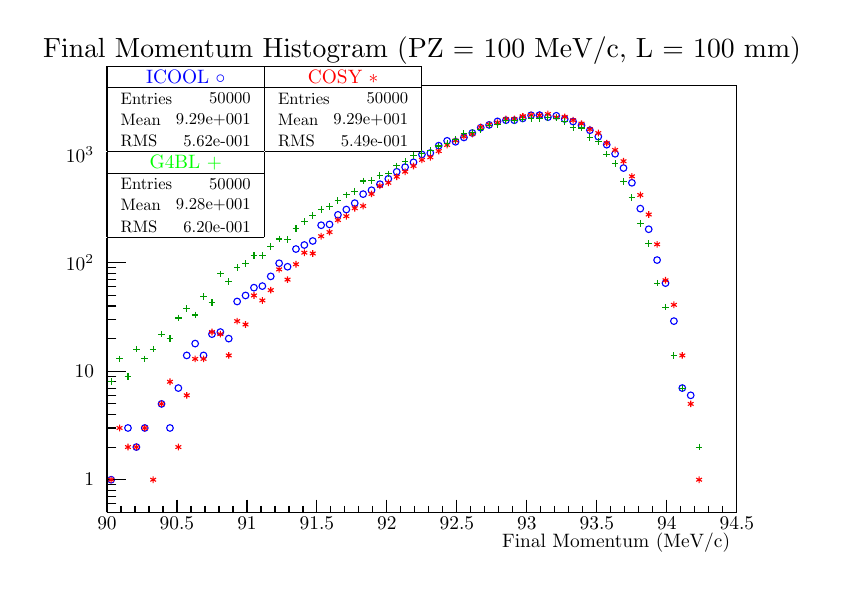
\begin{tikzpicture}
\definecolor{c}{rgb}{1,1,1};
\draw [color=c, fill=c] (0,0) rectangle (20,13.5632);
\draw [color=c, fill=c] (2,1.35632) rectangle (18,12.2069);
\definecolor{c}{rgb}{0,0,0};
\draw [c] (2,1.35632) -- (2,12.2069) -- (18,12.2069) -- (18,1.35632) -- (2,1.35632);
\definecolor{c}{rgb}{1,1,1};
\draw [color=c, fill=c] (2,1.35632) rectangle (18,12.2069);
\definecolor{c}{rgb}{0,0,0};
\draw [c] (2,1.35632) -- (2,12.2069) -- (18,12.2069) -- (18,1.35632) -- (2,1.35632);
\definecolor{c}{rgb}{0,0,1};
\foreach \P in
 {(2.10667,2.18552),(2.53333,3.49976),(2.74667,3.01472),(2.96,3.49976),(3.38667,4.11085),(3.6,3.49976),(3.81333,4.51337),(4.02667,5.34256),(4.24,5.64321),(4.45333,5.34256),(4.66667,5.88326),(4.88,5.93644),(5.09333,5.76925),(5.30667,6.71246),(5.52,6.8
6539),(5.73333,7.06339),(5.94667,7.10327),(6.16,7.35043),(6.37333,7.68256),(6.58667,7.59483),(6.8,8.0447),(7.01333,8.1473),(7.22667,8.24934),(7.44,8.64862),(7.65333,8.66998),(7.86667,8.91341),(8.08,9.04805),(8.29333,9.2102),(8.50667,9.43949),(8.72,9.
53824),(8.93333,9.69188),(9.14667,9.82801),(9.36,10.007),(9.57333,10.1255),(9.78667,10.2476),(10,10.4455),(10.2133,10.4845),(10.4267,10.6702),(10.64,10.793),(10.8533,10.7685),(11.0667,10.8787),(11.28,10.9925),(11.4933,11.1261),(11.7067,11.1979),(11.9
2,11.2867),(12.1333,11.3166),(12.3467,11.316),(12.56,11.362),(12.7733,11.4419),(12.9867,11.4424)}{\draw[mark options={color=c,fill=c},mark size=2.402402pt,mark=o] plot coordinates {\P};}
\foreach \P in
 {(12.9867,11.4424),(13.2,11.394),(13.4133,11.4293),(13.6267,11.3475),(13.84,11.2825),(14.0533,11.1863),(14.2667,11.0619),(14.48,10.8994),(14.6933,10.6948),(14.9067,10.4646),(15.12,10.1018),(15.3333,9.72739),(15.5467,9.07099),(15.76,8.54747),(15.9733
,7.76429),(16.1867,7.17925),(16.4,6.21374),(16.6133,4.51337),(16.8267,4.32896)}{\draw[mark options={color=c,fill=c},mark size=2.402402pt,mark=o] plot coordinates {\P};}
\definecolor{c}{rgb}{1,1,1};
\draw [color=c, fill=c] (2,10.5115) rectangle (6,12.6816);
\definecolor{c}{rgb}{0,0,0};
\draw [c] (2,10.5115) -- (6,10.5115);
\draw [c] (6,10.5115) -- (6,12.6816);
\draw [c] (6,12.6816) -- (2,12.6816);
\draw [c] (2,12.6816) -- (2,10.5115);
\draw[color=blue](4,12.4103) node[scale=0.7, rotate=0]{ICOOL $\circ$};
\draw [c] (2,12.1391) -- (6,12.1391);
\draw [anchor= west] (2.2,11.8678) node[scale=0.6, rotate=0]{Entries };
\draw [anchor= east] (5.8,11.8678) node[scale=0.6, rotate=0]{ 50000};
\draw [anchor= west] (2.2,11.3253) node[scale=0.6, rotate=0]{Mean  };
\draw [anchor= east] (5.8,11.3253) node[scale=0.6, rotate=0]{ 9.29e+001};
\draw [anchor= west] (2.2,10.7828) node[scale=0.6, rotate=0]{RMS   };
\draw [anchor= east] (5.8,10.7828) node[scale=0.6, rotate=0]{ 5.62e-001};
\draw [c] (2,1.35632) -- (18,1.35632);
\draw [anchor= east] (18,0.596782) node[scale=0.7, rotate=0]{Final Momentum (MeV/c)};
\draw [c] (2,1.68184) -- (2,1.35632);
\draw [c] (2.35556,1.51908) -- (2.35556,1.35632);
\draw [c] (2.71111,1.51908) -- (2.71111,1.35632);
\draw [c] (3.06667,1.51908) -- (3.06667,1.35632);
\draw [c] (3.42222,1.51908) -- (3.42222,1.35632);
\draw [c] (3.77778,1.68184) -- (3.77778,1.35632);
\draw [c] (4.13333,1.51908) -- (4.13333,1.35632);
\draw [c] (4.48889,1.51908) -- (4.48889,1.35632);
\draw [c] (4.84444,1.51908) -- (4.84444,1.35632);
\draw [c] (5.2,1.51908) -- (5.2,1.35632);
\draw [c] (5.55556,1.68184) -- (5.55556,1.35632);
\draw [c] (5.91111,1.51908) -- (5.91111,1.35632);
\draw [c] (6.26667,1.51908) -- (6.26667,1.35632);
\draw [c] (6.62222,1.51908) -- (6.62222,1.35632);
\draw [c] (6.97778,1.51908) -- (6.97778,1.35632);
\draw [c] (7.33333,1.68184) -- (7.33333,1.35632);
\draw [c] (7.68889,1.51908) -- (7.68889,1.35632);
\draw [c] (8.04444,1.51908) -- (8.04444,1.35632);
\draw [c] (8.4,1.51908) -- (8.4,1.35632);
\draw [c] (8.75556,1.51908) -- (8.75556,1.35632);
\draw [c] (9.11111,1.68184) -- (9.11111,1.35632);
\draw [c] (9.46667,1.51908) -- (9.46667,1.35632);
\draw [c] (9.82222,1.51908) -- (9.82222,1.35632);
\draw [c] (10.1778,1.51908) -- (10.1778,1.35632);
\draw [c] (10.5333,1.51908) -- (10.5333,1.35632);
\draw [c] (10.8889,1.68184) -- (10.8889,1.35632);
\draw [c] (11.2444,1.51908) -- (11.2444,1.35632);
\draw [c] (11.6,1.51908) -- (11.6,1.35632);
\draw [c] (11.9556,1.51908) -- (11.9556,1.35632);
\draw [c] (12.3111,1.51908) -- (12.3111,1.35632);
\draw [c] (12.6667,1.68184) -- (12.6667,1.35632);
\draw [c] (13.0222,1.51908) -- (13.0222,1.35632);
\draw [c] (13.3778,1.51908) -- (13.3778,1.35632);
\draw [c] (13.7333,1.51908) -- (13.7333,1.35632);
\draw [c] (14.0889,1.51908) -- (14.0889,1.35632);
\draw [c] (14.4444,1.68184) -- (14.4444,1.35632);
\draw [c] (14.8,1.51908) -- (14.8,1.35632);
\draw [c] (15.1556,1.51908) -- (15.1556,1.35632);
\draw [c] (15.5111,1.51908) -- (15.5111,1.35632);
\draw [c] (15.8667,1.51908) -- (15.8667,1.35632);
\draw [c] (16.2222,1.68184) -- (16.2222,1.35632);
\draw [c] (16.5778,1.51908) -- (16.5778,1.35632);
\draw [c] (16.9333,1.51908) -- (16.9333,1.35632);
\draw [c] (17.2889,1.51908) -- (17.2889,1.35632);
\draw [c] (17.6444,1.51908) -- (17.6444,1.35632);
\draw [c] (18,1.68184) -- (18,1.35632);
\draw [anchor=base] (2,0.908736) node[scale=0.7, rotate=0]{90};
\draw [anchor=base] (3.77778,0.908736) node[scale=0.7, rotate=0]{90.5};
\draw [anchor=base] (5.55556,0.908736) node[scale=0.7, rotate=0]{91};
\draw [anchor=base] (7.33333,0.908736) node[scale=0.7, rotate=0]{91.5};
\draw [anchor=base] (9.11111,0.908736) node[scale=0.7, rotate=0]{92};
\draw [anchor=base] (10.8889,0.908736) node[scale=0.7, rotate=0]{92.5};
\draw [anchor=base] (12.6667,0.908736) node[scale=0.7, rotate=0]{93};
\draw [anchor=base] (14.4444,0.908736) node[scale=0.7, rotate=0]{93.5};
\draw [anchor=base] (16.2222,0.908736) node[scale=0.7, rotate=0]{94};
\draw [anchor=base] (18,0.908736) node[scale=0.7, rotate=0]{94.5};
\draw [c] (2,1.35632) -- (2,12.2069);
\draw [c] (2.24,1.35632) -- (2,1.35632);
\draw [c] (2.24,1.57443) -- (2,1.57443);
\draw [c] (2.24,1.75884) -- (2,1.75884);
\draw [c] (2.24,1.91858) -- (2,1.91858);
\draw [c] (2.24,2.05948) -- (2,2.05948);
\draw [c] (2.48,2.18552) -- (2,2.18552);
\draw [anchor= east] (1.844,2.18552) node[scale=0.7, rotate=0]{1};
\draw [c] (2.24,3.01472) -- (2,3.01472);
\draw [c] (2.24,3.49977) -- (2,3.49977);
\draw [c] (2.24,3.84391) -- (2,3.84391);
\draw [c] (2.24,4.11086) -- (2,4.11086);
\draw [c] (2.24,4.32896) -- (2,4.32896);
\draw [c] (2.24,4.51337) -- (2,4.51337);
\draw [c] (2.24,4.67311) -- (2,4.67311);
\draw [c] (2.24,4.81401) -- (2,4.81401);
\draw [c] (2.48,4.94005) -- (2,4.94005);
\draw [anchor= east] (1.844,4.94005) node[scale=0.7, rotate=0]{10};
\draw [c] (2.24,5.76925) -- (2,5.76925);
\draw [c] (2.24,6.2543) -- (2,6.2543);
\draw [c] (2.24,6.59844) -- (2,6.59844);
\draw [c] (2.24,6.86539) -- (2,6.86539);
\draw [c] (2.24,7.08349) -- (2,7.08349);
\draw [c] (2.24,7.2679) -- (2,7.2679);
\draw [c] (2.24,7.42764) -- (2,7.42764);
\draw [c] (2.24,7.56854) -- (2,7.56854);
\draw [c] (2.48,7.69458) -- (2,7.69458);
\draw [anchor= east] (1.844,7.69458) node[scale=0.7, rotate=0]{$10^{2}$};
\draw [c] (2.24,8.52378) -- (2,8.52378);
\draw [c] (2.24,9.00883) -- (2,9.00883);
\draw [c] (2.24,9.35298) -- (2,9.35298);
\draw [c] (2.24,9.61992) -- (2,9.61992);
\draw [c] (2.24,9.83802) -- (2,9.83802);
\draw [c] (2.24,10.0224) -- (2,10.0224);
\draw [c] (2.24,10.1822) -- (2,10.1822);
\draw [c] (2.24,10.3231) -- (2,10.3231);
\draw [c] (2.48,10.4491) -- (2,10.4491);
\draw [anchor= east] (1.844,10.4491) node[scale=0.7, rotate=0]{$10^{3}$};
\draw [c] (2.24,11.2783) -- (2,11.2783);
\draw [c] (2.24,11.7634) -- (2,11.7634);
\draw [c] (2.24,12.1075) -- (2,12.1075);
\definecolor{c}{rgb}{1,1,1};
\draw [color=c, fill=c] (2,10.5115) rectangle (6,12.6816);
\definecolor{c}{rgb}{0,0,0};
\draw [c] (2,10.5115) -- (6,10.5115);
\draw [c] (6,10.5115) -- (6,12.6816);
\draw [c] (6,12.6816) -- (2,12.6816);
\draw [c] (2,12.6816) -- (2,10.5115);
\draw[color=blue](4,12.4103) node[scale=0.7, rotate=0]{ICOOL $\circ$};
\draw [c] (2,12.1391) -- (6,12.1391);
\draw [anchor= west] (2.2,11.8678) node[scale=0.6, rotate=0]{Entries };
\draw [anchor= east] (5.8,11.8678) node[scale=0.6, rotate=0]{ 50000};
\draw [anchor= west] (2.2,11.3253) node[scale=0.6, rotate=0]{Mean  };
\draw [anchor= east] (5.8,11.3253) node[scale=0.6, rotate=0]{ 9.29e+001};
\draw [anchor= west] (2.2,10.7828) node[scale=0.6, rotate=0]{RMS   };
\draw [anchor= east] (5.8,10.7828) node[scale=0.6, rotate=0]{ 5.62e-001};
\draw (10,13.0816) node[scale=1, rotate=0]{Final Momentum Histogram (PZ = 100 MeV/c, L = 100 mm)};
\definecolor{c}{rgb}{1,0,0};
\foreach \P in
 {(2.10667,2.18552),(2.32,3.49976),(2.53333,3.01472),(2.74667,3.01472),(2.96,3.49976),(3.17333,2.18552),(3.38667,4.11085),(3.6,4.67311),(3.81333,3.01472),(4.02667,4.32896),(4.24,5.25391),(4.45333,5.25391),(4.66667,5.93644),(4.88,5.88326),(5.09333,5.3
4256),(5.30667,6.21374),(5.52,6.12825),(5.73333,6.86539),(5.94667,6.73934),(6.16,7.00096),(6.37333,7.52799),(6.58667,7.2679),(6.8,7.65814),(7.01333,7.95191),(7.22667,7.93246),(7.44,8.37085),(7.65333,8.47494),(7.86667,8.78111),(8.08,8.87835),(8.29333,
9.08229),(8.50667,9.13726),(8.72,9.44504),(8.93333,9.64829),(9.14667,9.72739),(9.36,9.8811),(9.57333,10.0087),(9.78667,10.1549),(10,10.3084),(10.2133,10.3751),(10.4267,10.5323),(10.64,10.688),(10.8533,10.8028),(11.0667,10.9051),(11.28,10.9649),(11.49
33,11.1429),(11.7067,11.2043),(11.92,11.2554),(12.1333,11.3458),(12.3467,11.3486),(12.56,11.415)}{\draw[mark options={color=c,fill=c},mark size=2.402402pt,mark=asterisk] plot coordinates {\P};}
\foreach \P in
 {(12.56,11.415),(12.7733,11.4512),(12.9867,11.4403),(13.2,11.4733),(13.4133,11.3896),(13.6267,11.4021),(13.84,11.3166),(14.0533,11.2307),(14.2667,11.086),(14.48,10.9902),(14.6933,10.736),(14.9067,10.561),(15.12,10.2756),(15.3333,9.89068),(15.5467,9.
41702),(15.76,8.92201),(15.9733,8.16357),(16.1867,7.25069),(16.4,6.62798),(16.6133,5.34256),(16.8267,4.11085),(17.04,2.18552)}{\draw[mark options={color=c,fill=c},mark size=2.402402pt,mark=asterisk] plot coordinates {\P};}
\definecolor{c}{rgb}{1,1,1};
\draw [color=c, fill=c] (6,10.5115) rectangle (10,12.6816);
\definecolor{c}{rgb}{0,0,0};
\draw [c] (6,10.5115) -- (10,10.5115);
\draw [c] (10,10.5115) -- (10,12.6816);
\draw [c] (10,12.6816) -- (6,12.6816);
\draw [c] (6,12.6816) -- (6,10.5115);
\draw [color=red](8,12.4103) node[scale=0.7, rotate=0]{COSY $*$};
\draw [c] (6,12.1391) -- (10,12.1391);
\draw [anchor= west] (6.2,11.8678) node[scale=0.6, rotate=0]{Entries };
\draw [anchor= east] (9.8,11.8678) node[scale=0.6, rotate=0]{ 50000};
\draw [anchor= west] (6.2,11.3253) node[scale=0.6, rotate=0]{Mean  };
\draw [anchor= east] (9.8,11.3253) node[scale=0.6, rotate=0]{ 9.29e+001};
\draw [anchor= west] (6.2,10.7828) node[scale=0.6, rotate=0]{RMS   };
\draw [anchor= east] (9.8,10.7828) node[scale=0.6, rotate=0]{ 5.49e-001};
\definecolor{c}{rgb}{1,1,1};
\draw [color=c, fill=c] (6,10.5115) rectangle (10,12.6816);
\definecolor{c}{rgb}{0,0,0};
\draw [c] (6,10.5115) -- (10,10.5115);
\draw [c] (10,10.5115) -- (10,12.6816);
\draw [c] (10,12.6816) -- (6,12.6816);
\draw [c] (6,12.6816) -- (6,10.5115);
\draw [color=red](8,12.4103) node[scale=0.7, rotate=0]{COSY $*$};
\draw [c] (6,12.1391) -- (10,12.1391);
\draw [anchor= west] (6.2,11.8678) node[scale=0.6, rotate=0]{Entries };
\draw [anchor= east] (9.8,11.8678) node[scale=0.6, rotate=0]{ 50000};
\draw [anchor= west] (6.2,11.3253) node[scale=0.6, rotate=0]{Mean  };
\draw [anchor= east] (9.8,11.3253) node[scale=0.6, rotate=0]{ 9.29e+001};
\draw [anchor= west] (6.2,10.7828) node[scale=0.6, rotate=0]{RMS   };
\draw [anchor= east] (9.8,10.7828) node[scale=0.6, rotate=0]{ 5.49e-001};
\definecolor{c}{rgb}{0,0.6,0};
\foreach \P in
 {(2.10667,4.67311),(2.32,5.25391),(2.53333,4.81401),(2.74667,5.50231),(2.96,5.25391),(3.17333,5.50231),(3.38667,5.88326),(3.6,5.76925),(3.81333,6.29352),(4.02667,6.53708),(4.24,6.36831),(4.45333,6.84122),(4.66667,6.68496),(4.88,7.41259),(5.09333,7.2
155),(5.30667,7.56854),(5.52,7.67041),(5.73333,7.8824),(5.94667,7.8824),(6.16,8.10561),(6.37333,8.30088),(6.58667,8.29365),(6.8,8.55914),(7.01333,8.73689),(7.22667,8.89161),(7.44,9.05575),(7.65333,9.11921),(7.86667,9.27257),(8.08,9.41986),(8.29333,9.
51234),(8.50667,9.77246),(8.72,9.78711),(8.93333,9.91523),(9.14667,9.95204),(9.36,10.158),(9.57333,10.2756),(9.78667,10.4164),(10,10.4787),(10.2133,10.5489),(10.4267,10.6612),(10.64,10.7322),(10.8533,10.8344),(11.0667,10.9757),(11.28,11.0009),(11.493
3,11.074),(11.7067,11.1934),(11.92,11.2075),(12.1333,11.302),(12.3467,11.3108),(12.56,11.3441)}{\draw[mark options={color=c,fill=c},mark size=2.402402pt,mark=+] plot coordinates {\P};}
\foreach \P in
 {(12.56,11.3441),(12.7733,11.357),(12.9867,11.3508),(13.2,11.383),(13.4133,11.3693),(13.6267,11.2902),(13.84,11.122),(14.0533,11.1179),(14.2667,10.8812),(14.48,10.7821),(14.6933,10.4551),(14.9067,10.219),(15.12,9.76824),(15.3333,9.34698),(15.5467,8.
70133),(15.76,8.18758),(15.9733,7.17925),(16.1867,6.56816),(16.4,5.34256),(16.6133,4.51337),(17.04,3.01472)}{\draw[mark options={color=c,fill=c},mark size=2.402402pt,mark=+] plot coordinates {\P};}
\definecolor{c}{rgb}{1,1,1};
\draw [color=c, fill=c] (2,8.34138) rectangle (6,10.5115);
\definecolor{c}{rgb}{0,0,0};
\draw [c] (2,8.34138) -- (6,8.34138);
\draw [c] (6,8.34138) -- (6,10.5115);
\draw [c] (6,10.5115) -- (2,10.5115);
\draw [c] (2,10.5115) -- (2,8.34138);
\draw [color=green](4,10.2402) node[scale=0.7, rotate=0]{G4BL $+$};
\draw [c] (2,9.96897) -- (6,9.96897);
\draw [anchor= west] (2.2,9.6977) node[scale=0.6, rotate=0]{Entries };
\draw [anchor= east] (5.8,9.6977) node[scale=0.6, rotate=0]{ 50000};
\draw [anchor= west] (2.2,9.15517) node[scale=0.6, rotate=0]{Mean  };
\draw [anchor= east] (5.8,9.15517) node[scale=0.6, rotate=0]{ 9.28e+001};
\draw [anchor= west] (2.2,8.61264) node[scale=0.6, rotate=0]{RMS   };
\draw [anchor= east] (5.8,8.61264) node[scale=0.6, rotate=0]{ 6.20e-001};
\definecolor{c}{rgb}{1,1,1};
\draw [color=c, fill=c] (2,8.34138) rectangle (6,10.5115);
\definecolor{c}{rgb}{0,0,0};
\draw [c] (2,8.34138) -- (6,8.34138);
\draw [c] (6,8.34138) -- (6,10.5115);
\draw [c] (6,10.5115) -- (2,10.5115);
\draw [c] (2,10.5115) -- (2,8.34138);
\draw [color=green](4,10.2402) node[scale=0.7, rotate=0]{G4BL $+$};
\draw [c] (2,9.96897) -- (6,9.96897);
\draw [anchor= west] (2.2,9.6977) node[scale=0.6, rotate=0]{Entries };
\draw [anchor= east] (5.8,9.6977) node[scale=0.6, rotate=0]{ 50000};
\draw [anchor= west] (2.2,9.15517) node[scale=0.6, rotate=0]{Mean  };
\draw [anchor= east] (5.8,9.15517) node[scale=0.6, rotate=0]{ 9.28e+001};
\draw [anchor= west] (2.2,8.61264) node[scale=0.6, rotate=0]{RMS   };
\draw [anchor= east] (5.8,8.61264) node[scale=0.6, rotate=0]{ 6.20e-001};
\end{tikzpicture}
}\\
\frame{      \pgfdeclareplotmark{cross} {
\pgfpathmoveto{\pgfpoint{-0.3\pgfplotmarksize}{\pgfplotmarksize}}
\pgfpathlineto{\pgfpoint{+0.3\pgfplotmarksize}{\pgfplotmarksize}}
\pgfpathlineto{\pgfpoint{+0.3\pgfplotmarksize}{0.3\pgfplotmarksize}}
\pgfpathlineto{\pgfpoint{+1\pgfplotmarksize}{0.3\pgfplotmarksize}}
\pgfpathlineto{\pgfpoint{+1\pgfplotmarksize}{-0.3\pgfplotmarksize}}
\pgfpathlineto{\pgfpoint{+0.3\pgfplotmarksize}{-0.3\pgfplotmarksize}}
\pgfpathlineto{\pgfpoint{+0.3\pgfplotmarksize}{-1.\pgfplotmarksize}}
\pgfpathlineto{\pgfpoint{-0.3\pgfplotmarksize}{-1.\pgfplotmarksize}}
\pgfpathlineto{\pgfpoint{-0.3\pgfplotmarksize}{-0.3\pgfplotmarksize}}
\pgfpathlineto{\pgfpoint{-1.\pgfplotmarksize}{-0.3\pgfplotmarksize}}
\pgfpathlineto{\pgfpoint{-1.\pgfplotmarksize}{0.3\pgfplotmarksize}}
\pgfpathlineto{\pgfpoint{-0.3\pgfplotmarksize}{0.3\pgfplotmarksize}}
\pgfpathclose
\pgfusepathqstroke
}
\pgfdeclareplotmark{cross*} {
\pgfpathmoveto{\pgfpoint{-0.3\pgfplotmarksize}{\pgfplotmarksize}}
\pgfpathlineto{\pgfpoint{+0.3\pgfplotmarksize}{\pgfplotmarksize}}
\pgfpathlineto{\pgfpoint{+0.3\pgfplotmarksize}{0.3\pgfplotmarksize}}
\pgfpathlineto{\pgfpoint{+1\pgfplotmarksize}{0.3\pgfplotmarksize}}
\pgfpathlineto{\pgfpoint{+1\pgfplotmarksize}{-0.3\pgfplotmarksize}}
\pgfpathlineto{\pgfpoint{+0.3\pgfplotmarksize}{-0.3\pgfplotmarksize}}
\pgfpathlineto{\pgfpoint{+0.3\pgfplotmarksize}{-1.\pgfplotmarksize}}
\pgfpathlineto{\pgfpoint{-0.3\pgfplotmarksize}{-1.\pgfplotmarksize}}
\pgfpathlineto{\pgfpoint{-0.3\pgfplotmarksize}{-0.3\pgfplotmarksize}}
\pgfpathlineto{\pgfpoint{-1.\pgfplotmarksize}{-0.3\pgfplotmarksize}}
\pgfpathlineto{\pgfpoint{-1.\pgfplotmarksize}{0.3\pgfplotmarksize}}
\pgfpathlineto{\pgfpoint{-0.3\pgfplotmarksize}{0.3\pgfplotmarksize}}
\pgfpathclose
\pgfusepathqfillstroke
}
\pgfdeclareplotmark{newstar} {
\pgfpathmoveto{\pgfqpoint{0pt}{\pgfplotmarksize}}
\pgfpathlineto{\pgfqpointpolar{44}{0.5\pgfplotmarksize}}
\pgfpathlineto{\pgfqpointpolar{18}{\pgfplotmarksize}}
\pgfpathlineto{\pgfqpointpolar{-20}{0.5\pgfplotmarksize}}
\pgfpathlineto{\pgfqpointpolar{-54}{\pgfplotmarksize}}
\pgfpathlineto{\pgfqpointpolar{-90}{0.5\pgfplotmarksize}}
\pgfpathlineto{\pgfqpointpolar{234}{\pgfplotmarksize}}
\pgfpathlineto{\pgfqpointpolar{198}{0.5\pgfplotmarksize}}
\pgfpathlineto{\pgfqpointpolar{162}{\pgfplotmarksize}}
\pgfpathlineto{\pgfqpointpolar{134}{0.5\pgfplotmarksize}}
\pgfpathclose
\pgfusepathqstroke
}
\pgfdeclareplotmark{newstar*} {
\pgfpathmoveto{\pgfqpoint{0pt}{\pgfplotmarksize}}
\pgfpathlineto{\pgfqpointpolar{44}{0.5\pgfplotmarksize}}
\pgfpathlineto{\pgfqpointpolar{18}{\pgfplotmarksize}}
\pgfpathlineto{\pgfqpointpolar{-20}{0.5\pgfplotmarksize}}
\pgfpathlineto{\pgfqpointpolar{-54}{\pgfplotmarksize}}
\pgfpathlineto{\pgfqpointpolar{-90}{0.5\pgfplotmarksize}}
\pgfpathlineto{\pgfqpointpolar{234}{\pgfplotmarksize}}
\pgfpathlineto{\pgfqpointpolar{198}{0.5\pgfplotmarksize}}
\pgfpathlineto{\pgfqpointpolar{162}{\pgfplotmarksize}}
\pgfpathlineto{\pgfqpointpolar{134}{0.5\pgfplotmarksize}}
\pgfpathclose
\pgfusepathqfillstroke
}
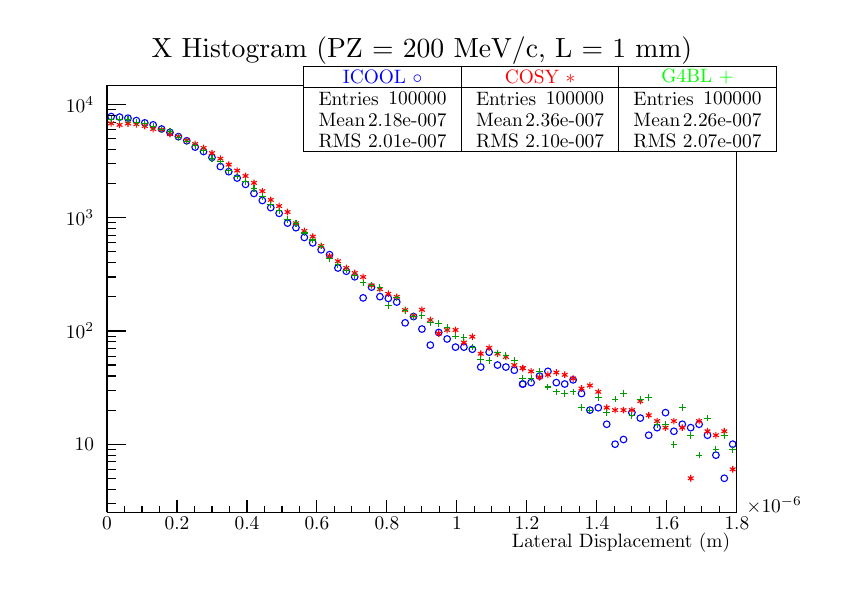
\begin{tikzpicture}
\definecolor{c}{rgb}{1,1,1};
\draw [color=c, fill=c] (0,0) rectangle (20,13.5632);
\draw [color=c, fill=c] (2,1.35632) rectangle (18,12.2069);
\definecolor{c}{rgb}{0,0,0};
\draw [c] (2,1.35632) -- (2,12.2069) -- (18,12.2069) -- (18,1.35632) -- (2,1.35632);
\definecolor{c}{rgb}{1,1,1};
\draw [color=c, fill=c] (2,1.35632) rectangle (18,12.2069);
\definecolor{c}{rgb}{0,0,0};
\draw [c] (2,1.35632) -- (2,12.2069) -- (18,12.2069) -- (18,1.35632) -- (2,1.35632);
\definecolor{c}{rgb}{0,0,1};
\foreach \P in
 {(2.10667,11.4087),(2.32,11.396),(2.53333,11.3685),(2.74667,11.3079),(2.96,11.249),(3.17333,11.1983),(3.38667,11.0937),(3.6,11.0072),(3.81333,10.8997),(4.02667,10.7946),(4.24,10.6344),(4.45333,10.5214),(4.66667,10.3726),(4.88,10.1395),(5.09333,10.01
),(5.30667,9.8483),(5.52,9.68748),(5.73333,9.45647),(5.94667,9.27733),(6.16,9.09691),(6.37333,8.95158),(6.58667,8.70362),(6.8,8.58694),(7.01333,8.3392),(7.22667,8.20138),(7.44,8.02505),(7.65333,7.90169),(7.86667,7.56338),(8.08,7.48093),(8.29333,7.339
83),(8.50667,6.80403),(8.72,7.07762),(8.93333,6.83549),(9.14667,6.79122),(9.36,6.69767),(9.57333,6.17028),(9.78667,6.32909),(10,6.01254),(10.2133,5.60426),(10.4267,5.92551),(10.64,5.76058),(10.8533,5.55327),(11.0667,5.55327),(11.28,5.50012),(11.4933,
5.04686),(11.7067,5.42553),(11.92,5.09785),(12.1333,5.04686),(12.3467,4.96626),(12.56,4.61617)}{\draw[mark options={color=c,fill=c},mark size=2.402402pt,mark=o] plot coordinates {\P};}
\foreach \P in
 {(12.56,4.61617),(12.7733,4.65238),(12.9867,4.81915),(13.2,4.93819),(13.4133,4.65238),(13.6267,4.61617),(13.84,4.72178),(14.0533,4.37368),(14.2667,3.95345),(14.48,4.01438),(14.6933,3.59414),(14.9067,3.08774),(15.12,3.20678),(15.3333,3.88938),(15.546
7,3.75047),(15.76,3.31545),(15.9733,3.50798),(16.1867,3.88938),(16.4,3.41542),(16.6133,3.59414),(16.8267,3.50798),(17.04,3.59414),(17.2533,3.31545),(17.4667,2.80904),(17.68,2.22203),(17.8933,3.08774)}{\draw[mark options={color=c,fill=c},mark
 size=2.402402pt,mark=o] plot coordinates {\P};}
\definecolor{c}{rgb}{1,1,1};
\draw [color=c, fill=c] (7,10.5115) rectangle (11,12.6816);
\definecolor{c}{rgb}{0,0,0};
\draw [c] (7,10.5115) -- (11,10.5115);
\draw [c] (11,10.5115) -- (11,12.6816);
\draw [c] (11,12.6816) -- (7,12.6816);
\draw [c] (7,12.6816) -- (7,10.5115);
\draw[color=blue](9,12.4103) node[scale=0.7, rotate=0]{ICOOL $\circ$};
\draw [c] (7,12.1391) -- (11,12.1391);
\draw [anchor= west] (7.2,11.8678) node[scale=0.7, rotate=0]{Entries };
\draw [anchor= east] (10.8,11.8678) node[scale=0.7, rotate=0]{ 100000};
\draw [anchor= west] (7.2,11.3253) node[scale=0.7, rotate=0]{Mean  };
\draw [anchor= east] (10.8,11.3253) node[scale=0.7, rotate=0]{ 2.18e-007};
\draw [anchor= west] (7.2,10.7828) node[scale=0.7, rotate=0]{RMS   };
\draw [anchor= east] (10.8,10.7828) node[scale=0.7, rotate=0]{ 2.01e-007};
\draw [c] (2,1.35632) -- (18,1.35632);
\draw [anchor= east] (18,0.596782) node[scale=0.7, rotate=0]{Lateral Displacement (m)};
\draw [c] (2,1.68184) -- (2,1.35632);
\draw [c] (2.44444,1.51908) -- (2.44444,1.35632);
\draw [c] (2.88889,1.51908) -- (2.88889,1.35632);
\draw [c] (3.33333,1.51908) -- (3.33333,1.35632);
\draw [c] (3.77778,1.68184) -- (3.77778,1.35632);
\draw [c] (4.22222,1.51908) -- (4.22222,1.35632);
\draw [c] (4.66667,1.51908) -- (4.66667,1.35632);
\draw [c] (5.11111,1.51908) -- (5.11111,1.35632);
\draw [c] (5.55556,1.68184) -- (5.55556,1.35632);
\draw [c] (6,1.51908) -- (6,1.35632);
\draw [c] (6.44444,1.51908) -- (6.44444,1.35632);
\draw [c] (6.88889,1.51908) -- (6.88889,1.35632);
\draw [c] (7.33333,1.68184) -- (7.33333,1.35632);
\draw [c] (7.77778,1.51908) -- (7.77778,1.35632);
\draw [c] (8.22222,1.51908) -- (8.22222,1.35632);
\draw [c] (8.66667,1.51908) -- (8.66667,1.35632);
\draw [c] (9.11111,1.68184) -- (9.11111,1.35632);
\draw [c] (9.55556,1.51908) -- (9.55556,1.35632);
\draw [c] (10,1.51908) -- (10,1.35632);
\draw [c] (10.4444,1.51908) -- (10.4444,1.35632);
\draw [c] (10.8889,1.68184) -- (10.8889,1.35632);
\draw [c] (11.3333,1.51908) -- (11.3333,1.35632);
\draw [c] (11.7778,1.51908) -- (11.7778,1.35632);
\draw [c] (12.2222,1.51908) -- (12.2222,1.35632);
\draw [c] (12.6667,1.68184) -- (12.6667,1.35632);
\draw [c] (13.1111,1.51908) -- (13.1111,1.35632);
\draw [c] (13.5556,1.51908) -- (13.5556,1.35632);
\draw [c] (14,1.51908) -- (14,1.35632);
\draw [c] (14.4444,1.68184) -- (14.4444,1.35632);
\draw [c] (14.8889,1.51908) -- (14.8889,1.35632);
\draw [c] (15.3333,1.51908) -- (15.3333,1.35632);
\draw [c] (15.7778,1.51908) -- (15.7778,1.35632);
\draw [c] (16.2222,1.68184) -- (16.2222,1.35632);
\draw [c] (16.6667,1.51908) -- (16.6667,1.35632);
\draw [c] (17.1111,1.51908) -- (17.1111,1.35632);
\draw [c] (17.5556,1.51908) -- (17.5556,1.35632);
\draw [c] (18,1.68184) -- (18,1.35632);
\draw [anchor=base] (2,0.908736) node[scale=0.7, rotate=0]{0};
\draw [anchor=base] (3.77778,0.908736) node[scale=0.7, rotate=0]{0.2};
\draw [anchor=base] (5.55556,0.908736) node[scale=0.7, rotate=0]{0.4};
\draw [anchor=base] (7.33333,0.908736) node[scale=0.7, rotate=0]{0.6};
\draw [anchor=base] (9.11111,0.908736) node[scale=0.7, rotate=0]{0.8};
\draw [anchor=base] (10.8889,0.908736) node[scale=0.7, rotate=0]{1};
\draw [anchor=base] (12.6667,0.908736) node[scale=0.7, rotate=0]{1.2};
\draw [anchor=base] (14.4444,0.908736) node[scale=0.7, rotate=0]{1.4};
\draw [anchor=base] (16.2222,0.908736) node[scale=0.7, rotate=0]{1.6};
\draw [anchor=base] (18,0.908736) node[scale=0.7, rotate=0]{1.8};
\draw [anchor=base west] (18.07,1.35632) node[scale=0.7, rotate=0]{$\times10^{-6}$};
\draw [c] (2,1.35632) -- (2,12.2069);
\draw [c] (2.24,1.58403) -- (2,1.58403);
\draw [c] (2.24,1.94333) -- (2,1.94333);
\draw [c] (2.24,2.22203) -- (2,2.22203);
\draw [c] (2.24,2.44974) -- (2,2.44974);
\draw [c] (2.24,2.64226) -- (2,2.64226);
\draw [c] (2.24,2.80904) -- (2,2.80904);
\draw [c] (2.24,2.95614) -- (2,2.95614);
\draw [c] (2.48,3.08774) -- (2,3.08774);
\draw [anchor= east] (1.844,3.08774) node[scale=0.7, rotate=0]{10};
\draw [c] (2.24,3.95344) -- (2,3.95344);
\draw [c] (2.24,4.45985) -- (2,4.45985);
\draw [c] (2.24,4.81915) -- (2,4.81915);
\draw [c] (2.24,5.09785) -- (2,5.09785);
\draw [c] (2.24,5.32556) -- (2,5.32556);
\draw [c] (2.24,5.51809) -- (2,5.51809);
\draw [c] (2.24,5.68486) -- (2,5.68486);
\draw [c] (2.24,5.83196) -- (2,5.83196);
\draw [c] (2.48,5.96356) -- (2,5.96356);
\draw [anchor= east] (1.844,5.96356) node[scale=0.7, rotate=0]{$10^{2}$};
\draw [c] (2.24,6.82926) -- (2,6.82926);
\draw [c] (2.24,7.33567) -- (2,7.33567);
\draw [c] (2.24,7.69497) -- (2,7.69497);
\draw [c] (2.24,7.97367) -- (2,7.97367);
\draw [c] (2.24,8.20138) -- (2,8.20138);
\draw [c] (2.24,8.3939) -- (2,8.3939);
\draw [c] (2.24,8.56068) -- (2,8.56068);
\draw [c] (2.24,8.70778) -- (2,8.70778);
\draw [c] (2.48,8.83938) -- (2,8.83938);
\draw [anchor= east] (1.844,8.83938) node[scale=0.7, rotate=0]{$10^{3}$};
\draw [c] (2.24,9.70508) -- (2,9.70508);
\draw [c] (2.24,10.2115) -- (2,10.2115);
\draw [c] (2.24,10.5708) -- (2,10.5708);
\draw [c] (2.24,10.8495) -- (2,10.8495);
\draw [c] (2.24,11.0772) -- (2,11.0772);
\draw [c] (2.24,11.2697) -- (2,11.2697);
\draw [c] (2.24,11.4365) -- (2,11.4365);
\draw [c] (2.24,11.5836) -- (2,11.5836);
\draw [c] (2.48,11.7152) -- (2,11.7152);
\draw [anchor= east] (1.844,11.7152) node[scale=0.7, rotate=0]{$10^{4}$};
\definecolor{c}{rgb}{1,1,1};
\draw [color=c, fill=c] (7,10.5115) rectangle (11,12.6816);
\definecolor{c}{rgb}{0,0,0};
\draw [c] (7,10.5115) -- (11,10.5115);
\draw [c] (11,10.5115) -- (11,12.6816);
\draw [c] (11,12.6816) -- (7,12.6816);
\draw [c] (7,12.6816) -- (7,10.5115);
\draw[color=blue](9,12.4103) node[scale=0.7, rotate=0]{ICOOL $\circ$};
\draw [c] (7,12.1391) -- (11,12.1391);
\draw [anchor= west] (7.2,11.8678) node[scale=0.7, rotate=0]{Entries };
\draw [anchor= east] (10.8,11.8678) node[scale=0.7, rotate=0]{ 100000};
\draw [anchor= west] (7.2,11.3253) node[scale=0.7, rotate=0]{Mean  };
\draw [anchor= east] (10.8,11.3253) node[scale=0.7, rotate=0]{ 2.18e-007};
\draw [anchor= west] (7.2,10.7828) node[scale=0.7, rotate=0]{RMS   };
\draw [anchor= east] (10.8,10.7828) node[scale=0.7, rotate=0]{ 2.01e-007};
\draw (10,13.0816) node[scale=1, rotate=0]{X Histogram (PZ = 200 MeV/c, L = 1 mm)};
\definecolor{c}{rgb}{1,0,0};
\foreach \P in
 {(2.10667,11.2381),(2.32,11.1979),(2.53333,11.2339),(2.74667,11.2145),(2.96,11.1691),(3.17333,11.0923),(3.38667,11.0787),(3.6,10.9637),(3.81333,10.9011),(4.02667,10.7993),(4.24,10.7121),(4.45333,10.6125),(4.66667,10.4812),(4.88,10.3407),(5.09333,10.
1892),(5.30667,10.0366),(5.52,9.90011),(5.73333,9.72614),(5.94667,9.51453),(6.16,9.29132),(6.37333,9.13593),(6.58667,8.98426),(6.8,8.69943),(7.01333,8.50481),(7.22667,8.35954),(7.44,8.1241),(7.65333,7.86409),(7.86667,7.73492),(8.08,7.56338),(8.29333,
7.43564),(8.50667,7.33567),(8.72,7.12286),(8.93333,7.02535),(9.14667,6.90792),(9.36,6.82926),(9.57333,6.4947),(9.78667,6.34759),(10,6.50283),(10.2133,6.24225),(10.4267,5.89949),(10.64,5.98829),(10.8533,5.98829),(11.0667,5.66915),(11.28,5.81801),(11.4
933,5.3865),(11.7067,5.5358),(11.92,5.3865),(12.1333,5.30457),(12.3467,5.09785),(12.56,5.02057)}{\draw[mark options={color=c,fill=c},mark size=2.402402pt,mark=asterisk] plot coordinates {\P};}
\foreach \P in
 {(12.56,5.02057),(12.7733,4.93819),(12.9867,4.78753),(13.2,4.84999),(13.4133,4.90948),(13.6267,4.84999),(13.84,4.75509),(14.0533,4.5008),(14.2667,4.57889),(14.48,4.41751),(14.6933,4.01438),(14.9067,3.95345),(15.12,3.95345),(15.3333,3.95345),(15.5467
,4.18116),(15.76,3.82186),(15.9733,3.67475),(16.1867,3.50798),(16.4,3.67475),(16.6133,3.50798),(16.8267,2.22203),(17.04,3.67475),(17.2533,3.41542),(17.4667,3.31545),(17.68,3.41542),(17.8933,2.44974)}{\draw[mark options={color=c,fill=c},mark
 size=2.402402pt,mark=asterisk] plot coordinates {\P};}
\definecolor{c}{rgb}{1,1,1};
\draw [color=c, fill=c] (11,10.5115) rectangle (15,12.6816);
\definecolor{c}{rgb}{0,0,0};
\draw [c] (11,10.5115) -- (15,10.5115);
\draw [c] (15,10.5115) -- (15,12.6816);
\draw [c] (15,12.6816) -- (11,12.6816);
\draw [c] (11,12.6816) -- (11,10.5115);
\draw [color=red](13,12.4103) node[scale=0.7, rotate=0]{COSY $*$};
\draw [c] (11,12.1391) -- (15,12.1391);
\draw [anchor= west] (11.2,11.8678) node[scale=0.7, rotate=0]{Entries };
\draw [anchor= east] (14.8,11.8678) node[scale=0.7, rotate=0]{ 100000};
\draw [anchor= west] (11.2,11.3253) node[scale=0.7, rotate=0]{Mean  };
\draw [anchor= east] (14.8,11.3253) node[scale=0.7, rotate=0]{ 2.36e-007};
\draw [anchor= west] (11.2,10.7828) node[scale=0.7, rotate=0]{RMS   };
\draw [anchor= east] (14.8,10.7828) node[scale=0.7, rotate=0]{ 2.10e-007};
\definecolor{c}{rgb}{1,1,1};
\draw [color=c, fill=c] (11,10.5115) rectangle (15,12.6816);
\definecolor{c}{rgb}{0,0,0};
\draw [c] (11,10.5115) -- (15,10.5115);
\draw [c] (15,10.5115) -- (15,12.6816);
\draw [c] (15,12.6816) -- (11,12.6816);
\draw [c] (11,12.6816) -- (11,10.5115);
\draw [color=red](13,12.4103) node[scale=0.7, rotate=0]{COSY $*$};
\draw [c] (11,12.1391) -- (15,12.1391);
\draw [anchor= west] (11.2,11.8678) node[scale=0.7, rotate=0]{Entries };
\draw [anchor= east] (14.8,11.8678) node[scale=0.7, rotate=0]{ 100000};
\draw [anchor= west] (11.2,11.3253) node[scale=0.7, rotate=0]{Mean  };
\draw [anchor= east] (14.8,11.3253) node[scale=0.7, rotate=0]{ 2.36e-007};
\draw [anchor= west] (11.2,10.7828) node[scale=0.7, rotate=0]{RMS   };
\draw [anchor= east] (14.8,10.7828) node[scale=0.7, rotate=0]{ 2.10e-007};
\definecolor{c}{rgb}{0,0.6,0};
\foreach \P in
 {(2.10667,11.3386),(2.32,11.3364),(2.53333,11.3313),(2.74667,11.2563),(2.96,11.235),(3.17333,11.151),(3.38667,11.0807),(3.6,11.04),(3.81333,10.8732),(4.02667,10.7698),(4.24,10.6747),(4.45333,10.5411),(4.66667,10.3497),(4.88,10.2577),(5.09333,10.0332
),(5.30667,9.8969),(5.52,9.75407),(5.73333,9.58455),(5.94667,9.37459),(6.16,9.18139),(6.37333,9.01502),(6.58667,8.80133),(6.8,8.69243),(7.01333,8.45314),(7.22667,8.27415),(7.44,8.11966),(7.65333,7.79398),(7.86667,7.65048),(8.08,7.51023),(8.29333,7.36
854),(8.50667,7.18544),(8.72,7.12779),(8.93333,7.06734),(9.14667,6.61151),(9.36,6.80403),(9.57333,6.48651),(9.78667,6.33837),(10,6.35674),(10.2133,6.18082),(10.4267,6.14893),(10.64,6.05968),(10.8533,5.83197),(11.0667,5.8039),(11.28,5.55327),(11.4933,
5.23939),(11.7067,5.21689),(11.92,5.40617),(12.1333,5.3462),(12.3467,5.21689),(12.56,4.75509)}{\draw[mark options={color=c,fill=c},mark size=2.402402pt,mark=+] plot coordinates {\P};}
\foreach \P in
 {(12.56,4.75509),(12.7733,4.75509),(12.9867,4.93819),(13.2,4.54046),(13.4133,4.41751),(13.6267,4.37368),(13.84,4.41751),(14.0533,4.01438),(14.2667,3.95345),(14.48,4.28113),(14.6933,3.88938),(14.9067,4.23214),(15.12,4.37368),(15.3333,3.82186),(15.546
7,4.23214),(15.76,4.28113),(15.9733,3.59414),(16.1867,3.59414),(16.4,3.08774),(16.6133,4.01438),(16.8267,3.31545),(17.04,2.80904),(17.2533,3.75047),(17.4667,2.95615),(17.68,3.31545),(17.8933,2.95615)}{\draw[mark options={color=c,fill=c},mark
 size=2.402402pt,mark=+] plot coordinates {\P};}
\definecolor{c}{rgb}{1,1,1};
\draw [color=c, fill=c] (15,10.5115) rectangle (19,12.6816);
\definecolor{c}{rgb}{0,0,0};
\draw [c] (15,10.5115) -- (19,10.5115);
\draw [c] (19,10.5115) -- (19,12.6816);
\draw [c] (19,12.6816) -- (15,12.6816);
\draw [c] (15,12.6816) -- (15,10.5115);
\draw [color=green](17,12.4103) node[scale=0.7, rotate=0]{G4BL $+$};
\draw [c] (15,12.1391) -- (19,12.1391);
\draw [anchor= west] (15.2,11.8678) node[scale=0.7, rotate=0]{Entries };
\draw [anchor= east] (18.8,11.8678) node[scale=0.7, rotate=0]{ 100000};
\draw [anchor= west] (15.2,11.3253) node[scale=0.7, rotate=0]{Mean  };
\draw [anchor= east] (18.8,11.3253) node[scale=0.7, rotate=0]{ 2.26e-007};
\draw [anchor= west] (15.2,10.7828) node[scale=0.7, rotate=0]{RMS   };
\draw [anchor= east] (18.8,10.7828) node[scale=0.7, rotate=0]{ 2.07e-007};
\definecolor{c}{rgb}{1,1,1};
\draw [color=c, fill=c] (15,10.5115) rectangle (19,12.6816);
\definecolor{c}{rgb}{0,0,0};
\draw [c] (15,10.5115) -- (19,10.5115);
\draw [c] (19,10.5115) -- (19,12.6816);
\draw [c] (19,12.6816) -- (15,12.6816);
\draw [c] (15,12.6816) -- (15,10.5115);
\draw [color=green](17,12.4103) node[scale=0.7, rotate=0]{G4BL $+$};
\draw [c] (15,12.1391) -- (19,12.1391);
\draw [anchor= west] (15.2,11.8678) node[scale=0.7, rotate=0]{Entries };
\draw [anchor= east] (18.8,11.8678) node[scale=0.7, rotate=0]{ 100000};
\draw [anchor= west] (15.2,11.3253) node[scale=0.7, rotate=0]{Mean  };
\draw [anchor= east] (18.8,11.3253) node[scale=0.7, rotate=0]{ 2.26e-007};
\draw [anchor= west] (15.2,10.7828) node[scale=0.7, rotate=0]{RMS   };
\draw [anchor= east] (18.8,10.7828) node[scale=0.7, rotate=0]{ 2.07e-007};
\end{tikzpicture}
}\\
\frame{    \pgfdeclareplotmark{cross} {
\pgfpathmoveto{\pgfpoint{-0.3\pgfplotmarksize}{\pgfplotmarksize}}
\pgfpathlineto{\pgfpoint{+0.3\pgfplotmarksize}{\pgfplotmarksize}}
\pgfpathlineto{\pgfpoint{+0.3\pgfplotmarksize}{0.3\pgfplotmarksize}}
\pgfpathlineto{\pgfpoint{+1\pgfplotmarksize}{0.3\pgfplotmarksize}}
\pgfpathlineto{\pgfpoint{+1\pgfplotmarksize}{-0.3\pgfplotmarksize}}
\pgfpathlineto{\pgfpoint{+0.3\pgfplotmarksize}{-0.3\pgfplotmarksize}}
\pgfpathlineto{\pgfpoint{+0.3\pgfplotmarksize}{-1.\pgfplotmarksize}}
\pgfpathlineto{\pgfpoint{-0.3\pgfplotmarksize}{-1.\pgfplotmarksize}}
\pgfpathlineto{\pgfpoint{-0.3\pgfplotmarksize}{-0.3\pgfplotmarksize}}
\pgfpathlineto{\pgfpoint{-1.\pgfplotmarksize}{-0.3\pgfplotmarksize}}
\pgfpathlineto{\pgfpoint{-1.\pgfplotmarksize}{0.3\pgfplotmarksize}}
\pgfpathlineto{\pgfpoint{-0.3\pgfplotmarksize}{0.3\pgfplotmarksize}}
\pgfpathclose
\pgfusepathqstroke
}
\pgfdeclareplotmark{cross*} {
\pgfpathmoveto{\pgfpoint{-0.3\pgfplotmarksize}{\pgfplotmarksize}}
\pgfpathlineto{\pgfpoint{+0.3\pgfplotmarksize}{\pgfplotmarksize}}
\pgfpathlineto{\pgfpoint{+0.3\pgfplotmarksize}{0.3\pgfplotmarksize}}
\pgfpathlineto{\pgfpoint{+1\pgfplotmarksize}{0.3\pgfplotmarksize}}
\pgfpathlineto{\pgfpoint{+1\pgfplotmarksize}{-0.3\pgfplotmarksize}}
\pgfpathlineto{\pgfpoint{+0.3\pgfplotmarksize}{-0.3\pgfplotmarksize}}
\pgfpathlineto{\pgfpoint{+0.3\pgfplotmarksize}{-1.\pgfplotmarksize}}
\pgfpathlineto{\pgfpoint{-0.3\pgfplotmarksize}{-1.\pgfplotmarksize}}
\pgfpathlineto{\pgfpoint{-0.3\pgfplotmarksize}{-0.3\pgfplotmarksize}}
\pgfpathlineto{\pgfpoint{-1.\pgfplotmarksize}{-0.3\pgfplotmarksize}}
\pgfpathlineto{\pgfpoint{-1.\pgfplotmarksize}{0.3\pgfplotmarksize}}
\pgfpathlineto{\pgfpoint{-0.3\pgfplotmarksize}{0.3\pgfplotmarksize}}
\pgfpathclose
\pgfusepathqfillstroke
}
\pgfdeclareplotmark{newstar} {
\pgfpathmoveto{\pgfqpoint{0pt}{\pgfplotmarksize}}
\pgfpathlineto{\pgfqpointpolar{44}{0.5\pgfplotmarksize}}
\pgfpathlineto{\pgfqpointpolar{18}{\pgfplotmarksize}}
\pgfpathlineto{\pgfqpointpolar{-20}{0.5\pgfplotmarksize}}
\pgfpathlineto{\pgfqpointpolar{-54}{\pgfplotmarksize}}
\pgfpathlineto{\pgfqpointpolar{-90}{0.5\pgfplotmarksize}}
\pgfpathlineto{\pgfqpointpolar{234}{\pgfplotmarksize}}
\pgfpathlineto{\pgfqpointpolar{198}{0.5\pgfplotmarksize}}
\pgfpathlineto{\pgfqpointpolar{162}{\pgfplotmarksize}}
\pgfpathlineto{\pgfqpointpolar{134}{0.5\pgfplotmarksize}}
\pgfpathclose
\pgfusepathqstroke
}
\pgfdeclareplotmark{newstar*} {
\pgfpathmoveto{\pgfqpoint{0pt}{\pgfplotmarksize}}
\pgfpathlineto{\pgfqpointpolar{44}{0.5\pgfplotmarksize}}
\pgfpathlineto{\pgfqpointpolar{18}{\pgfplotmarksize}}
\pgfpathlineto{\pgfqpointpolar{-20}{0.5\pgfplotmarksize}}
\pgfpathlineto{\pgfqpointpolar{-54}{\pgfplotmarksize}}
\pgfpathlineto{\pgfqpointpolar{-90}{0.5\pgfplotmarksize}}
\pgfpathlineto{\pgfqpointpolar{234}{\pgfplotmarksize}}
\pgfpathlineto{\pgfqpointpolar{198}{0.5\pgfplotmarksize}}
\pgfpathlineto{\pgfqpointpolar{162}{\pgfplotmarksize}}
\pgfpathlineto{\pgfqpointpolar{134}{0.5\pgfplotmarksize}}
\pgfpathclose
\pgfusepathqfillstroke
}
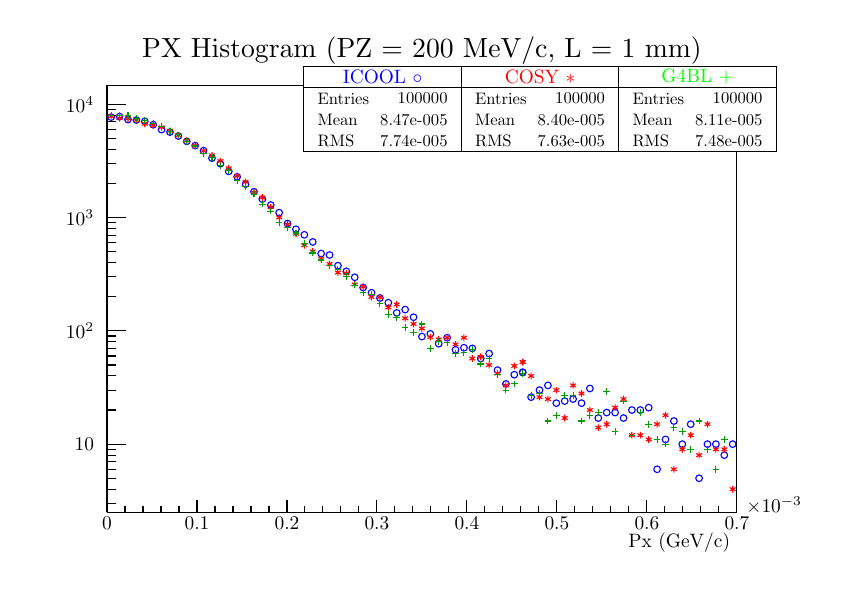
\begin{tikzpicture}
\definecolor{c}{rgb}{1,1,1};
\draw [color=c, fill=c] (0,0) rectangle (20,13.5632);
\draw [color=c, fill=c] (2,1.35632) rectangle (18,12.2069);
\definecolor{c}{rgb}{0,0,0};
\draw [c] (2,1.35632) -- (2,12.2069) -- (18,12.2069) -- (18,1.35632) -- (2,1.35632);
\definecolor{c}{rgb}{1,1,1};
\draw [color=c, fill=c] (2,1.35632) rectangle (18,12.2069);
\definecolor{c}{rgb}{0,0,0};
\draw [c] (2,1.35632) -- (2,12.2069) -- (18,12.2069) -- (18,1.35632) -- (2,1.35632);
\definecolor{c}{rgb}{0,0,1};
\foreach \P in
 {(2.10667,11.3952),(2.32,11.4081),(2.53333,11.3343),(2.74667,11.3216),(2.96,11.2877),(3.17333,11.2024),(3.38667,11.0788),(3.6,11.016),(3.81333,10.9159),(4.02667,10.7798),(4.24,10.6719),(4.45333,10.5442),(4.66667,10.3525),(4.88,10.2112),(5.09333,10.0
172),(5.30667,9.87818),(5.52,9.6935),(5.73333,9.49989),(5.94667,9.31178),(6.16,9.16209),(6.37333,8.96845),(6.58667,8.69351),(6.8,8.547),(7.01333,8.40612),(7.22667,8.22494),(7.44,7.93004),(7.65333,7.89312),(7.86667,7.62222),(8.08,7.47792),(8.29333,7.3
2744),(8.50667,7.0663),(8.72,6.93519),(8.93333,6.80158),(9.14667,6.68053),(9.36,6.42264),(9.57333,6.50656),(9.78667,6.31389),(10,5.82124),(10.2133,5.88956),(10.4267,5.64022),(10.64,5.79283),(10.8533,5.48487),(11.0667,5.53883),(11.28,5.5211),(11.4933,
5.26432),(11.7067,5.38941),(11.92,4.96887),(12.1333,4.61853),(12.3467,4.85252),(12.56,4.91205)}{\draw[mark options={color=c,fill=c},mark size=2.402402pt,mark=o] plot coordinates {\P};}
\foreach \P in
 {(12.56,4.91205),(12.7733,4.28324),(12.9867,4.4621),(13.2,4.58122),(13.4133,4.13001),(13.6267,4.1832),(13.84,4.23422),(14.0533,4.13001),(14.2667,4.50308),(14.48,3.7522),(14.6933,3.89122),(14.9067,3.89122),(15.12,3.7522),(15.3333,3.95532),(15.5467,3.
95532),(15.76,4.01631),(15.9733,2.45053),(16.1867,3.20811),(16.4,3.67643),(16.6133,3.08899),(16.8267,3.59576),(17.04,2.22266),(17.2533,3.08899),(17.4667,3.08899),(17.68,2.81009),(17.8933,3.08899)}{\draw[mark options={color=c,fill=c},mark
 size=2.402402pt,mark=o] plot coordinates {\P};}
\definecolor{c}{rgb}{1,1,1};
\draw [color=c, fill=c] (7,10.5115) rectangle (11,12.6816);
\definecolor{c}{rgb}{0,0,0};
\draw [c] (7,10.5115) -- (11,10.5115);
\draw [c] (11,10.5115) -- (11,12.6816);
\draw [c] (11,12.6816) -- (7,12.6816);
\draw [c] (7,12.6816) -- (7,10.5115);
\draw[color=blue](9,12.4103) node[scale=0.7, rotate=0]{ICOOL $\circ$};
\draw [c] (7,12.1391) -- (11,12.1391);
\draw [anchor= west] (7.2,11.8678) node[scale=0.6, rotate=0]{Entries };
\draw [anchor= east] (10.8,11.8678) node[scale=0.6, rotate=0]{ 100000};
\draw [anchor= west] (7.2,11.3253) node[scale=0.6, rotate=0]{Mean  };
\draw [anchor= east] (10.8,11.3253) node[scale=0.6, rotate=0]{ 8.47e-005};
\draw [anchor= west] (7.2,10.7828) node[scale=0.6, rotate=0]{RMS   };
\draw [anchor= east] (10.8,10.7828) node[scale=0.6, rotate=0]{ 7.74e-005};
\draw [c] (2,1.35632) -- (18,1.35632);
\draw [anchor= east] (18,0.596782) node[scale=0.7, rotate=0]{Px (GeV/c)};
\draw [c] (2,1.68184) -- (2,1.35632);
\draw [c] (2.45714,1.51908) -- (2.45714,1.35632);
\draw [c] (2.91429,1.51908) -- (2.91429,1.35632);
\draw [c] (3.37143,1.51908) -- (3.37143,1.35632);
\draw [c] (3.82857,1.51908) -- (3.82857,1.35632);
\draw [c] (4.28571,1.68184) -- (4.28571,1.35632);
\draw [c] (4.74286,1.51908) -- (4.74286,1.35632);
\draw [c] (5.2,1.51908) -- (5.2,1.35632);
\draw [c] (5.65714,1.51908) -- (5.65714,1.35632);
\draw [c] (6.11429,1.51908) -- (6.11429,1.35632);
\draw [c] (6.57143,1.68184) -- (6.57143,1.35632);
\draw [c] (7.02857,1.51908) -- (7.02857,1.35632);
\draw [c] (7.48571,1.51908) -- (7.48571,1.35632);
\draw [c] (7.94286,1.51908) -- (7.94286,1.35632);
\draw [c] (8.4,1.51908) -- (8.4,1.35632);
\draw [c] (8.85714,1.68184) -- (8.85714,1.35632);
\draw [c] (9.31429,1.51908) -- (9.31429,1.35632);
\draw [c] (9.77143,1.51908) -- (9.77143,1.35632);
\draw [c] (10.2286,1.51908) -- (10.2286,1.35632);
\draw [c] (10.6857,1.51908) -- (10.6857,1.35632);
\draw [c] (11.1429,1.68184) -- (11.1429,1.35632);
\draw [c] (11.6,1.51908) -- (11.6,1.35632);
\draw [c] (12.0571,1.51908) -- (12.0571,1.35632);
\draw [c] (12.5143,1.51908) -- (12.5143,1.35632);
\draw [c] (12.9714,1.51908) -- (12.9714,1.35632);
\draw [c] (13.4286,1.68184) -- (13.4286,1.35632);
\draw [c] (13.8857,1.51908) -- (13.8857,1.35632);
\draw [c] (14.3429,1.51908) -- (14.3429,1.35632);
\draw [c] (14.8,1.51908) -- (14.8,1.35632);
\draw [c] (15.2571,1.51908) -- (15.2571,1.35632);
\draw [c] (15.7143,1.68184) -- (15.7143,1.35632);
\draw [c] (16.1714,1.51908) -- (16.1714,1.35632);
\draw [c] (16.6286,1.51908) -- (16.6286,1.35632);
\draw [c] (17.0857,1.51908) -- (17.0857,1.35632);
\draw [c] (17.5429,1.51908) -- (17.5429,1.35632);
\draw [c] (18,1.68184) -- (18,1.35632);
\draw [c] (18,1.68184) -- (18,1.35632);
\draw [anchor=base] (2,0.908736) node[scale=0.7, rotate=0]{0};
\draw [anchor=base] (4.28571,0.908736) node[scale=0.7, rotate=0]{0.1};
\draw [anchor=base] (6.57143,0.908736) node[scale=0.7, rotate=0]{0.2};
\draw [anchor=base] (8.85714,0.908736) node[scale=0.7, rotate=0]{0.3};
\draw [anchor=base] (11.1429,0.908736) node[scale=0.7, rotate=0]{0.4};
\draw [anchor=base] (13.4286,0.908736) node[scale=0.7, rotate=0]{0.5};
\draw [anchor=base] (15.7143,0.908736) node[scale=0.7, rotate=0]{0.6};
\draw [anchor=base] (18,0.908736) node[scale=0.7, rotate=0]{0.7};
\draw [anchor=base west] (18.07,1.35632) node[scale=0.7, rotate=0]{$\times10^{-3}$};
\draw [c] (2,1.35632) -- (2,12.2069);
\draw [c] (2.24,1.58419) -- (2,1.58419);
\draw [c] (2.24,1.94376) -- (2,1.94376);
\draw [c] (2.24,2.22265) -- (2,2.22265);
\draw [c] (2.24,2.45053) -- (2,2.45053);
\draw [c] (2.24,2.6432) -- (2,2.6432);
\draw [c] (2.24,2.81009) -- (2,2.81009);
\draw [c] (2.24,2.9573) -- (2,2.9573);
\draw [c] (2.48,3.08899) -- (2,3.08899);
\draw [anchor= east] (1.844,3.08899) node[scale=0.7, rotate=0]{10};
\draw [c] (2.24,3.95532) -- (2,3.95532);
\draw [c] (2.24,4.4621) -- (2,4.4621);
\draw [c] (2.24,4.82166) -- (2,4.82166);
\draw [c] (2.24,5.10055) -- (2,5.10055);
\draw [c] (2.24,5.32843) -- (2,5.32843);
\draw [c] (2.24,5.5211) -- (2,5.5211);
\draw [c] (2.24,5.68799) -- (2,5.68799);
\draw [c] (2.24,5.8352) -- (2,5.8352);
\draw [c] (2.48,5.96689) -- (2,5.96689);
\draw [anchor= east] (1.844,5.96689) node[scale=0.7, rotate=0]{$10^{2}$};
\draw [c] (2.24,6.83322) -- (2,6.83322);
\draw [c] (2.24,7.34) -- (2,7.34);
\draw [c] (2.24,7.69956) -- (2,7.69956);
\draw [c] (2.24,7.97846) -- (2,7.97846);
\draw [c] (2.24,8.20633) -- (2,8.20633);
\draw [c] (2.24,8.399) -- (2,8.399);
\draw [c] (2.24,8.56589) -- (2,8.56589);
\draw [c] (2.24,8.71311) -- (2,8.71311);
\draw [c] (2.48,8.84479) -- (2,8.84479);
\draw [anchor= east] (1.844,8.84479) node[scale=0.7, rotate=0]{$10^{3}$};
\draw [c] (2.24,9.71112) -- (2,9.71112);
\draw [c] (2.24,10.2179) -- (2,10.2179);
\draw [c] (2.24,10.5775) -- (2,10.5775);
\draw [c] (2.24,10.8564) -- (2,10.8564);
\draw [c] (2.24,11.0842) -- (2,11.0842);
\draw [c] (2.24,11.2769) -- (2,11.2769);
\draw [c] (2.24,11.4438) -- (2,11.4438);
\draw [c] (2.24,11.591) -- (2,11.591);
\draw [c] (2.48,11.7227) -- (2,11.7227);
\draw [anchor= east] (1.844,11.7227) node[scale=0.7, rotate=0]{$10^{4}$};
\definecolor{c}{rgb}{1,1,1};
\draw [color=c, fill=c] (7,10.5115) rectangle (11,12.6816);
\definecolor{c}{rgb}{0,0,0};
\draw [c] (7,10.5115) -- (11,10.5115);
\draw [c] (11,10.5115) -- (11,12.6816);
\draw [c] (11,12.6816) -- (7,12.6816);
\draw [c] (7,12.6816) -- (7,10.5115);
\draw[color=blue](9,12.4103) node[scale=0.7, rotate=0]{ICOOL $\circ$};
\draw [c] (7,12.1391) -- (11,12.1391);
\draw [anchor= west] (7.2,11.8678) node[scale=0.6, rotate=0]{Entries };
\draw [anchor= east] (10.8,11.8678) node[scale=0.6, rotate=0]{ 100000};
\draw [anchor= west] (7.2,11.3253) node[scale=0.6, rotate=0]{Mean  };
\draw [anchor= east] (10.8,11.3253) node[scale=0.6, rotate=0]{ 8.47e-005};
\draw [anchor= west] (7.2,10.7828) node[scale=0.6, rotate=0]{RMS   };
\draw [anchor= east] (10.8,10.7828) node[scale=0.6, rotate=0]{ 7.74e-005};
\draw (10,13.0816) node[scale=1, rotate=0]{PX Histogram (PZ = 200 MeV/c, L = 1 mm)};
\definecolor{c}{rgb}{1,0,0};
\foreach \P in
 {(2.10667,11.4173),(2.32,11.367),(2.53333,11.3608),(2.74667,11.3194),(2.96,11.2283),(3.17333,11.1883),(3.38667,11.1365),(3.6,11.0468),(3.81333,10.9348),(4.02667,10.7965),(4.24,10.6687),(4.45333,10.541),(4.66667,10.4234),(4.88,10.2781),(5.09333,10.09
45),(5.30667,9.90254),(5.52,9.75049),(5.73333,9.48275),(5.94667,9.35406),(6.16,9.10353),(6.37333,8.84854),(6.58667,8.6693),(6.8,8.43247),(7.01333,8.14003),(7.22667,7.98345),(7.44,7.79285),(7.65333,7.66471),(7.86667,7.44771),(8.08,7.42456),(8.29333,7.
14664),(8.50667,7.08687),(8.72,6.82696),(8.93333,6.82066),(9.14667,6.56212),(9.36,6.63743),(9.57333,6.28516),(9.78667,6.14157),(10,6.02787),(10.2133,5.80712),(10.4267,5.74897),(10.64,5.79283),(10.8533,5.62388),(11.0667,5.79283),(11.28,5.26432),(11.49
33,5.30743),(11.7067,5.10056),(11.92,4.88264),(12.1333,4.58122),(12.3467,5.07531),(12.56,5.17338)}{\draw[mark options={color=c,fill=c},mark size=2.402402pt,mark=asterisk] plot coordinates {\P};}
\foreach \P in
 {(12.56,5.17338),(12.7733,4.82166),(12.9867,4.28324),(13.2,4.23422),(13.4133,4.4621),(13.6267,3.7522),(13.84,4.58122),(14.0533,4.37587),(14.2667,3.95532),(14.48,3.50953),(14.6933,3.59576),(14.9067,4.01631),(15.12,4.23422),(15.3333,3.31687),(15.5467,
3.31687),(15.76,3.20811),(15.9733,3.59576),(16.1867,3.82364),(16.4,2.45053),(16.6133,2.9573),(16.8267,3.31687),(17.04,2.81009),(17.2533,3.59576),(17.4667,2.9573),(17.68,2.9573),(17.8933,1.94376)}{\draw[mark options={color=c,fill=c},mark
 size=2.402402pt,mark=asterisk] plot coordinates {\P};}
\definecolor{c}{rgb}{1,1,1};
\draw [color=c, fill=c] (11,10.5115) rectangle (15,12.6816);
\definecolor{c}{rgb}{0,0,0};
\draw [c] (11,10.5115) -- (15,10.5115);
\draw [c] (15,10.5115) -- (15,12.6816);
\draw [c] (15,12.6816) -- (11,12.6816);
\draw [c] (11,12.6816) -- (11,10.5115);
\draw [color=red](13,12.4103) node[scale=0.7, rotate=0]{COSY $*$};
\draw [c] (11,12.1391) -- (15,12.1391);
\draw [anchor= west] (11.2,11.8678) node[scale=0.6, rotate=0]{Entries };
\draw [anchor= east] (14.8,11.8678) node[scale=0.6, rotate=0]{ 100000};
\draw [anchor= west] (11.2,11.3253) node[scale=0.6, rotate=0]{Mean  };
\draw [anchor= east] (14.8,11.3253) node[scale=0.6, rotate=0]{ 8.40e-005};
\draw [anchor= west] (11.2,10.7828) node[scale=0.6, rotate=0]{RMS   };
\draw [anchor= east] (14.8,10.7828) node[scale=0.6, rotate=0]{ 7.63e-005};
\definecolor{c}{rgb}{1,1,1};
\draw [color=c, fill=c] (11,10.5115) rectangle (15,12.6816);
\definecolor{c}{rgb}{0,0,0};
\draw [c] (11,10.5115) -- (15,10.5115);
\draw [c] (15,10.5115) -- (15,12.6816);
\draw [c] (15,12.6816) -- (11,12.6816);
\draw [c] (11,12.6816) -- (11,10.5115);
\draw [color=red](13,12.4103) node[scale=0.7, rotate=0]{COSY $*$};
\draw [c] (11,12.1391) -- (15,12.1391);
\draw [anchor= west] (11.2,11.8678) node[scale=0.6, rotate=0]{Entries };
\draw [anchor= east] (14.8,11.8678) node[scale=0.6, rotate=0]{ 100000};
\draw [anchor= west] (11.2,11.3253) node[scale=0.6, rotate=0]{Mean  };
\draw [anchor= east] (14.8,11.3253) node[scale=0.6, rotate=0]{ 8.40e-005};
\draw [anchor= west] (11.2,10.7828) node[scale=0.6, rotate=0]{RMS   };
\draw [anchor= east] (14.8,10.7828) node[scale=0.6, rotate=0]{ 7.63e-005};
\definecolor{c}{rgb}{0,0.6,0};
\foreach \P in
 {(2.10667,11.4471),(2.32,11.4334),(2.53333,11.4309),(2.74667,11.3558),(2.96,11.3025),(3.17333,11.2368),(3.38667,11.1545),(3.6,11.0371),(3.81333,10.9426),(4.02667,10.7804),(4.24,10.6626),(4.45333,10.4661),(4.66667,10.3743),(4.88,10.1708),(5.09333,10.
0284),(5.30667,9.77864),(5.52,9.62779),(5.73333,9.44002),(5.94667,9.18515),(6.16,9.00856),(6.37333,8.72279),(6.58667,8.58142),(6.8,8.45316),(7.01333,8.18321),(7.22667,7.94296),(7.44,7.76648),(7.65333,7.6189),(7.86667,7.5183),(8.08,7.35243),(8.29333,7
.12703),(8.50667,6.93519),(8.72,6.88824),(8.93333,6.65917),(9.14667,6.38743),(9.36,6.29481),(9.57333,6.05145),(9.78667,5.92882),(10,6.14157),(10.2133,5.5211),(10.4267,5.68799),(10.64,5.67227),(10.8533,5.38941),(11.0667,5.4091),(11.28,5.48487),(11.493
3,5.12531),(11.7067,5.26432),(11.92,4.85252),(12.1333,4.4621),(12.3467,4.61853),(12.56,4.88264)}{\draw[mark options={color=c,fill=c},mark size=2.402402pt,mark=+] plot coordinates {\P};}
\foreach \P in
 {(12.56,4.88264),(12.7733,4.33041),(12.9867,4.37587),(13.2,3.67643),(13.4133,3.82364),(13.6267,4.33041),(13.84,4.33041),(14.0533,3.67643),(14.2667,3.82364),(14.48,3.89122),(14.6933,4.41973),(14.9067,3.41691),(15.12,4.1832),(15.3333,3.31687),(15.5467
,3.89122),(15.76,3.59576),(15.9733,3.20811),(16.1867,3.08899),(16.4,3.50953),(16.6133,3.41691),(16.8267,2.9573),(17.04,3.67643),(17.2533,2.9573),(17.4667,2.45053),(17.68,3.20811)}{\draw[mark options={color=c,fill=c},mark size=2.402402pt,mark=+] plot
 coordinates {\P};}
\definecolor{c}{rgb}{1,1,1};
\draw [color=c, fill=c] (15,10.5115) rectangle (19,12.6816);
\definecolor{c}{rgb}{0,0,0};
\draw [c] (15,10.5115) -- (19,10.5115);
\draw [c] (19,10.5115) -- (19,12.6816);
\draw [c] (19,12.6816) -- (15,12.6816);
\draw [c] (15,12.6816) -- (15,10.5115);
\draw [color=green](17,12.4103) node[scale=0.7, rotate=0]{G4BL $+$};
\draw [c] (15,12.1391) -- (19,12.1391);
\draw [anchor= west] (15.2,11.8678) node[scale=0.6, rotate=0]{Entries };
\draw [anchor= east] (18.8,11.8678) node[scale=0.6, rotate=0]{ 100000};
\draw [anchor= west] (15.2,11.3253) node[scale=0.6, rotate=0]{Mean  };
\draw [anchor= east] (18.8,11.3253) node[scale=0.6, rotate=0]{ 8.11e-005};
\draw [anchor= west] (15.2,10.7828) node[scale=0.6, rotate=0]{RMS   };
\draw [anchor= east] (18.8,10.7828) node[scale=0.6, rotate=0]{ 7.48e-005};
\definecolor{c}{rgb}{1,1,1};
\draw [color=c, fill=c] (15,10.5115) rectangle (19,12.6816);
\definecolor{c}{rgb}{0,0,0};
\draw [c] (15,10.5115) -- (19,10.5115);
\draw [c] (19,10.5115) -- (19,12.6816);
\draw [c] (19,12.6816) -- (15,12.6816);
\draw [c] (15,12.6816) -- (15,10.5115);
\draw [color=green](17,12.4103) node[scale=0.7, rotate=0]{G4BL $+$};
\draw [c] (15,12.1391) -- (19,12.1391);
\draw [anchor= west] (15.2,11.8678) node[scale=0.6, rotate=0]{Entries };
\draw [anchor= east] (18.8,11.8678) node[scale=0.6, rotate=0]{ 100000};
\draw [anchor= west] (15.2,11.3253) node[scale=0.6, rotate=0]{Mean  };
\draw [anchor= east] (18.8,11.3253) node[scale=0.6, rotate=0]{ 8.11e-005};
\draw [anchor= west] (15.2,10.7828) node[scale=0.6, rotate=0]{RMS   };
\draw [anchor= east] (18.8,10.7828) node[scale=0.6, rotate=0]{ 7.48e-005};
\end{tikzpicture}
}\\
\frame{\pgfdeclareplotmark{cross} {
\pgfpathmoveto{\pgfpoint{-0.3\pgfplotmarksize}{\pgfplotmarksize}}
\pgfpathlineto{\pgfpoint{+0.3\pgfplotmarksize}{\pgfplotmarksize}}
\pgfpathlineto{\pgfpoint{+0.3\pgfplotmarksize}{0.3\pgfplotmarksize}}
\pgfpathlineto{\pgfpoint{+1\pgfplotmarksize}{0.3\pgfplotmarksize}}
\pgfpathlineto{\pgfpoint{+1\pgfplotmarksize}{-0.3\pgfplotmarksize}}
\pgfpathlineto{\pgfpoint{+0.3\pgfplotmarksize}{-0.3\pgfplotmarksize}}
\pgfpathlineto{\pgfpoint{+0.3\pgfplotmarksize}{-1.\pgfplotmarksize}}
\pgfpathlineto{\pgfpoint{-0.3\pgfplotmarksize}{-1.\pgfplotmarksize}}
\pgfpathlineto{\pgfpoint{-0.3\pgfplotmarksize}{-0.3\pgfplotmarksize}}
\pgfpathlineto{\pgfpoint{-1.\pgfplotmarksize}{-0.3\pgfplotmarksize}}
\pgfpathlineto{\pgfpoint{-1.\pgfplotmarksize}{0.3\pgfplotmarksize}}
\pgfpathlineto{\pgfpoint{-0.3\pgfplotmarksize}{0.3\pgfplotmarksize}}
\pgfpathclose
\pgfusepathqstroke
}
\pgfdeclareplotmark{cross*} {
\pgfpathmoveto{\pgfpoint{-0.3\pgfplotmarksize}{\pgfplotmarksize}}
\pgfpathlineto{\pgfpoint{+0.3\pgfplotmarksize}{\pgfplotmarksize}}
\pgfpathlineto{\pgfpoint{+0.3\pgfplotmarksize}{0.3\pgfplotmarksize}}
\pgfpathlineto{\pgfpoint{+1\pgfplotmarksize}{0.3\pgfplotmarksize}}
\pgfpathlineto{\pgfpoint{+1\pgfplotmarksize}{-0.3\pgfplotmarksize}}
\pgfpathlineto{\pgfpoint{+0.3\pgfplotmarksize}{-0.3\pgfplotmarksize}}
\pgfpathlineto{\pgfpoint{+0.3\pgfplotmarksize}{-1.\pgfplotmarksize}}
\pgfpathlineto{\pgfpoint{-0.3\pgfplotmarksize}{-1.\pgfplotmarksize}}
\pgfpathlineto{\pgfpoint{-0.3\pgfplotmarksize}{-0.3\pgfplotmarksize}}
\pgfpathlineto{\pgfpoint{-1.\pgfplotmarksize}{-0.3\pgfplotmarksize}}
\pgfpathlineto{\pgfpoint{-1.\pgfplotmarksize}{0.3\pgfplotmarksize}}
\pgfpathlineto{\pgfpoint{-0.3\pgfplotmarksize}{0.3\pgfplotmarksize}}
\pgfpathclose
\pgfusepathqfillstroke
}
\pgfdeclareplotmark{newstar} {
\pgfpathmoveto{\pgfqpoint{0pt}{\pgfplotmarksize}}
\pgfpathlineto{\pgfqpointpolar{44}{0.5\pgfplotmarksize}}
\pgfpathlineto{\pgfqpointpolar{18}{\pgfplotmarksize}}
\pgfpathlineto{\pgfqpointpolar{-20}{0.5\pgfplotmarksize}}
\pgfpathlineto{\pgfqpointpolar{-54}{\pgfplotmarksize}}
\pgfpathlineto{\pgfqpointpolar{-90}{0.5\pgfplotmarksize}}
\pgfpathlineto{\pgfqpointpolar{234}{\pgfplotmarksize}}
\pgfpathlineto{\pgfqpointpolar{198}{0.5\pgfplotmarksize}}
\pgfpathlineto{\pgfqpointpolar{162}{\pgfplotmarksize}}
\pgfpathlineto{\pgfqpointpolar{134}{0.5\pgfplotmarksize}}
\pgfpathclose
\pgfusepathqstroke
}
\pgfdeclareplotmark{newstar*} {
\pgfpathmoveto{\pgfqpoint{0pt}{\pgfplotmarksize}}
\pgfpathlineto{\pgfqpointpolar{44}{0.5\pgfplotmarksize}}
\pgfpathlineto{\pgfqpointpolar{18}{\pgfplotmarksize}}
\pgfpathlineto{\pgfqpointpolar{-20}{0.5\pgfplotmarksize}}
\pgfpathlineto{\pgfqpointpolar{-54}{\pgfplotmarksize}}
\pgfpathlineto{\pgfqpointpolar{-90}{0.5\pgfplotmarksize}}
\pgfpathlineto{\pgfqpointpolar{234}{\pgfplotmarksize}}
\pgfpathlineto{\pgfqpointpolar{198}{0.5\pgfplotmarksize}}
\pgfpathlineto{\pgfqpointpolar{162}{\pgfplotmarksize}}
\pgfpathlineto{\pgfqpointpolar{134}{0.5\pgfplotmarksize}}
\pgfpathclose
\pgfusepathqfillstroke
}
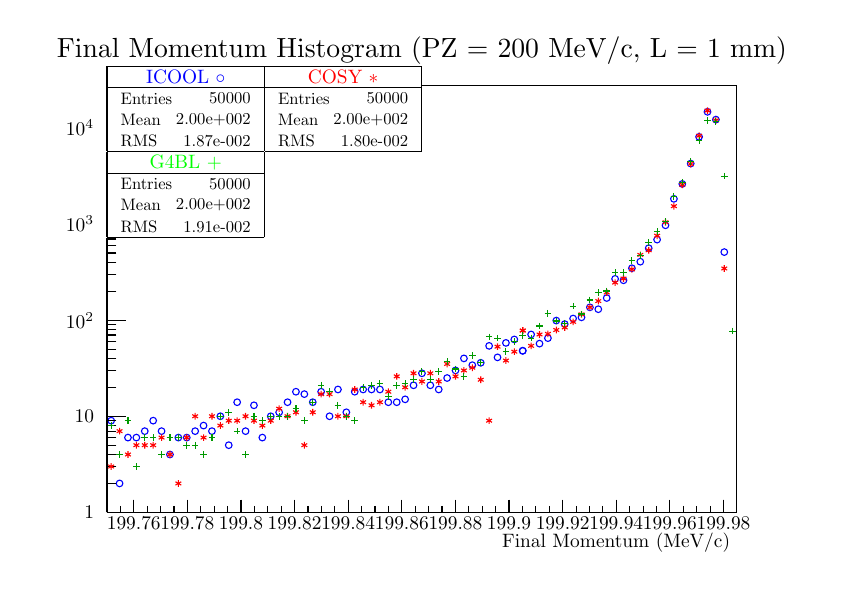
\begin{tikzpicture}
\definecolor{c}{rgb}{1,1,1};
\draw [color=c, fill=c] (0,0) rectangle (20,13.5632);
\draw [color=c, fill=c] (2,1.35632) rectangle (18,12.2069);
\definecolor{c}{rgb}{0,0,0};
\draw [c] (2,1.35632) -- (2,12.2069) -- (18,12.2069) -- (18,1.35632) -- (2,1.35632);
\definecolor{c}{rgb}{1,1,1};
\draw [color=c, fill=c] (2,1.35632) rectangle (18,12.2069);
\definecolor{c}{rgb}{0,0,0};
\draw [c] (2,1.35632) -- (2,12.2069) -- (18,12.2069) -- (18,1.35632) -- (2,1.35632);
\definecolor{c}{rgb}{0,0,1};
\foreach \P in
 {(2.10667,3.68552),(2.32,2.0911),(2.53333,3.2557),(2.74667,3.2557),(2.96,3.41911),(3.17333,3.68552),(3.38667,3.41911),(3.6,2.82588),(3.81333,3.2557),(4.02667,3.2557),(4.24,3.41911),(4.45333,3.56066),(4.66667,3.41911),(4.88,3.79721),(5.09333,3.06243)
,(5.30667,4.15389),(5.52,3.41911),(5.73333,4.07533),(5.94667,3.2557),(6.16,3.79721),(6.37333,3.89824),(6.58667,4.15389),(6.8,4.4203),(7.01333,4.35971),(7.22667,4.15389),(7.44,4.4203),(7.65333,3.79721),(7.86667,4.47762),(8.08,3.89824),(8.29333,4.4203)
,(8.50667,4.47762),(8.72,4.47762),(8.93333,4.47762),(9.14667,4.15389),(9.36,4.15389),(9.57333,4.22703),(9.78667,4.58371),(10,4.88867),(10.2133,4.58371),(10.4267,4.47762),(10.64,4.76854),(10.8533,4.96181),(11.0667,5.26677),(11.28,5.09449),(11.4933,5.1
5508),(11.7067,5.5849),(11.92,5.29295),(12.1333,5.66065),(12.3467,5.74831),(12.56,5.46004)}{\draw[mark options={color=c,fill=c},mark size=2.402402pt,mark=o] plot coordinates {\P};}
\foreach \P in
 {(12.56,5.46004),(12.7733,5.87504),(12.9867,5.64222),(13.2,5.78144),(13.4133,6.22744),(13.6267,6.13812),(13.84,6.27967),(14.0533,6.30982),(14.2667,6.56405),(14.48,6.51622),(14.6933,6.8006),(14.9067,7.28708),(15.12,7.251),(15.3333,7.55698),(15.5467,7
.72344),(15.76,8.06623),(15.9733,8.2841),(16.1867,8.64779),(16.4,9.3196),(16.6133,9.69839),(16.8267,10.2163),(17.04,10.8941),(17.2533,11.5294),(17.4667,11.3321),(17.68,7.96727)}{\draw[mark options={color=c,fill=c},mark size=2.402402pt,mark=o] plot
 coordinates {\P};}
\definecolor{c}{rgb}{1,1,1};
\draw [color=c, fill=c] (2,10.5115) rectangle (6,12.6816);
\definecolor{c}{rgb}{0,0,0};
\draw [c] (2,10.5115) -- (6,10.5115);
\draw [c] (6,10.5115) -- (6,12.6816);
\draw [c] (6,12.6816) -- (2,12.6816);
\draw [c] (2,12.6816) -- (2,10.5115);
\draw[color=blue](4,12.4103) node[scale=0.7, rotate=0]{ICOOL $\circ$};
\draw [c] (2,12.1391) -- (6,12.1391);
\draw [anchor= west] (2.2,11.8678) node[scale=0.6, rotate=0]{Entries };
\draw [anchor= east] (5.8,11.8678) node[scale=0.6, rotate=0]{ 50000};
\draw [anchor= west] (2.2,11.3253) node[scale=0.6, rotate=0]{Mean  };
\draw [anchor= east] (5.8,11.3253) node[scale=0.6, rotate=0]{ 2.00e+002};
\draw [anchor= west] (2.2,10.7828) node[scale=0.6, rotate=0]{RMS   };
\draw [anchor= east] (5.8,10.7828) node[scale=0.6, rotate=0]{ 1.87e-002};
\draw [c] (2,1.35632) -- (18,1.35632);
\draw [anchor= east] (18,0.596782) node[scale=0.7, rotate=0]{Final Momentum (MeV/c)};
\draw [c] (2.68085,1.68184) -- (2.68085,1.35632);
\draw [c] (3.02128,1.51908) -- (3.02128,1.35632);
\draw [c] (3.3617,1.51908) -- (3.3617,1.35632);
\draw [c] (3.70213,1.51908) -- (3.70213,1.35632);
\draw [c] (4.04255,1.68184) -- (4.04255,1.35632);
\draw [c] (4.38298,1.51908) -- (4.38298,1.35632);
\draw [c] (4.7234,1.51908) -- (4.7234,1.35632);
\draw [c] (5.06383,1.51908) -- (5.06383,1.35632);
\draw [c] (5.40426,1.68184) -- (5.40426,1.35632);
\draw [c] (5.74468,1.51908) -- (5.74468,1.35632);
\draw [c] (6.08511,1.51908) -- (6.08511,1.35632);
\draw [c] (6.42553,1.51908) -- (6.42553,1.35632);
\draw [c] (6.76596,1.68184) -- (6.76596,1.35632);
\draw [c] (7.10638,1.51908) -- (7.10638,1.35632);
\draw [c] (7.44681,1.51908) -- (7.44681,1.35632);
\draw [c] (7.78723,1.51908) -- (7.78723,1.35632);
\draw [c] (8.12766,1.68184) -- (8.12766,1.35632);
\draw [c] (8.46809,1.51908) -- (8.46809,1.35632);
\draw [c] (8.80851,1.51908) -- (8.80851,1.35632);
\draw [c] (9.14894,1.51908) -- (9.14894,1.35632);
\draw [c] (9.48936,1.68184) -- (9.48936,1.35632);
\draw [c] (9.82979,1.51908) -- (9.82979,1.35632);
\draw [c] (10.1702,1.51908) -- (10.1702,1.35632);
\draw [c] (10.5106,1.51908) -- (10.5106,1.35632);
\draw [c] (10.8511,1.68184) -- (10.8511,1.35632);
\draw [c] (11.1915,1.51908) -- (11.1915,1.35632);
\draw [c] (11.5319,1.51908) -- (11.5319,1.35632);
\draw [c] (11.8723,1.51908) -- (11.8723,1.35632);
\draw [c] (12.2128,1.68184) -- (12.2128,1.35632);
\draw [c] (12.5532,1.51908) -- (12.5532,1.35632);
\draw [c] (12.8936,1.51908) -- (12.8936,1.35632);
\draw [c] (13.234,1.51908) -- (13.234,1.35632);
\draw [c] (13.5745,1.68184) -- (13.5745,1.35632);
\draw [c] (13.9149,1.51908) -- (13.9149,1.35632);
\draw [c] (14.2553,1.51908) -- (14.2553,1.35632);
\draw [c] (14.5957,1.51908) -- (14.5957,1.35632);
\draw [c] (14.9362,1.68184) -- (14.9362,1.35632);
\draw [c] (15.2766,1.51908) -- (15.2766,1.35632);
\draw [c] (15.617,1.51908) -- (15.617,1.35632);
\draw [c] (15.9574,1.51908) -- (15.9574,1.35632);
\draw [c] (16.2979,1.68184) -- (16.2979,1.35632);
\draw [c] (16.6383,1.51908) -- (16.6383,1.35632);
\draw [c] (16.9787,1.51908) -- (16.9787,1.35632);
\draw [c] (17.3191,1.51908) -- (17.3191,1.35632);
\draw [c] (17.6596,1.68184) -- (17.6596,1.35632);
\draw [c] (2.68085,1.68184) -- (2.68085,1.35632);
\draw [c] (2.34043,1.51908) -- (2.34043,1.35632);
\draw [c] (2,1.51908) -- (2,1.35632);
\draw [c] (17.6596,1.68184) -- (17.6596,1.35632);
\draw [c] (18,1.51908) -- (18,1.35632);
\draw [anchor=base] (2.68085,0.908736) node[scale=0.7, rotate=0]{199.76};
\draw [anchor=base] (4.04255,0.908736) node[scale=0.7, rotate=0]{199.78};
\draw [anchor=base] (5.40426,0.908736) node[scale=0.7, rotate=0]{199.8};
\draw [anchor=base] (6.76596,0.908736) node[scale=0.7, rotate=0]{199.82};
\draw [anchor=base] (8.12766,0.908736) node[scale=0.7, rotate=0]{199.84};
\draw [anchor=base] (9.48936,0.908736) node[scale=0.7, rotate=0]{199.86};
\draw [anchor=base] (10.8511,0.908736) node[scale=0.7, rotate=0]{199.88};
\draw [anchor=base] (12.2128,0.908736) node[scale=0.7, rotate=0]{199.9};
\draw [anchor=base] (13.5745,0.908736) node[scale=0.7, rotate=0]{199.92};
\draw [anchor=base] (14.9362,0.908736) node[scale=0.7, rotate=0]{199.94};
\draw [anchor=base] (16.2979,0.908736) node[scale=0.7, rotate=0]{199.96};
\draw [anchor=base] (17.6596,0.908736) node[scale=0.7, rotate=0]{199.98};
\draw [c] (2,1.35632) -- (2,12.2069);
\draw [c] (2.48,1.35632) -- (2,1.35632);
\draw [anchor= east] (1.844,1.35632) node[scale=0.7, rotate=0]{1};
\draw [c] (2.24,2.0911) -- (2,2.0911);
\draw [c] (2.24,2.52092) -- (2,2.52092);
\draw [c] (2.24,2.82589) -- (2,2.82589);
\draw [c] (2.24,3.06243) -- (2,3.06243);
\draw [c] (2.24,3.2557) -- (2,3.2557);
\draw [c] (2.24,3.41911) -- (2,3.41911);
\draw [c] (2.24,3.56067) -- (2,3.56067);
\draw [c] (2.24,3.68552) -- (2,3.68552);
\draw [c] (2.48,3.79721) -- (2,3.79721);
\draw [anchor= east] (1.844,3.79721) node[scale=0.7, rotate=0]{10};
\draw [c] (2.24,4.53199) -- (2,4.53199);
\draw [c] (2.24,4.96181) -- (2,4.96181);
\draw [c] (2.24,5.26677) -- (2,5.26677);
\draw [c] (2.24,5.50332) -- (2,5.50332);
\draw [c] (2.24,5.69659) -- (2,5.69659);
\draw [c] (2.24,5.86) -- (2,5.86);
\draw [c] (2.24,6.00155) -- (2,6.00155);
\draw [c] (2.24,6.12641) -- (2,6.12641);
\draw [c] (2.48,6.2381) -- (2,6.2381);
\draw [anchor= east] (1.844,6.2381) node[scale=0.7, rotate=0]{$10^{2}$};
\draw [c] (2.24,6.97288) -- (2,6.97288);
\draw [c] (2.24,7.4027) -- (2,7.4027);
\draw [c] (2.24,7.70766) -- (2,7.70766);
\draw [c] (2.24,7.94421) -- (2,7.94421);
\draw [c] (2.24,8.13748) -- (2,8.13748);
\draw [c] (2.24,8.30089) -- (2,8.30089);
\draw [c] (2.24,8.44244) -- (2,8.44244);
\draw [c] (2.24,8.5673) -- (2,8.5673);
\draw [c] (2.48,8.67899) -- (2,8.67899);
\draw [anchor= east] (1.844,8.67899) node[scale=0.7, rotate=0]{$10^{3}$};
\draw [c] (2.24,9.41377) -- (2,9.41377);
\draw [c] (2.24,9.84359) -- (2,9.84359);
\draw [c] (2.24,10.1485) -- (2,10.1485);
\draw [c] (2.24,10.3851) -- (2,10.3851);
\draw [c] (2.24,10.5784) -- (2,10.5784);
\draw [c] (2.24,10.7418) -- (2,10.7418);
\draw [c] (2.24,10.8833) -- (2,10.8833);
\draw [c] (2.24,11.0082) -- (2,11.0082);
\draw [c] (2.48,11.1199) -- (2,11.1199);
\draw [anchor= east] (1.844,11.1199) node[scale=0.7, rotate=0]{$10^{4}$};
\draw [c] (2.24,11.8547) -- (2,11.8547);
\definecolor{c}{rgb}{1,1,1};
\draw [color=c, fill=c] (2,10.5115) rectangle (6,12.6816);
\definecolor{c}{rgb}{0,0,0};
\draw [c] (2,10.5115) -- (6,10.5115);
\draw [c] (6,10.5115) -- (6,12.6816);
\draw [c] (6,12.6816) -- (2,12.6816);
\draw [c] (2,12.6816) -- (2,10.5115);
\draw[color=blue](4,12.4103) node[scale=0.7, rotate=0]{ICOOL $\circ$};
\draw [c] (2,12.1391) -- (6,12.1391);
\draw [anchor= west] (2.2,11.8678) node[scale=0.6, rotate=0]{Entries };
\draw [anchor= east] (5.8,11.8678) node[scale=0.6, rotate=0]{ 50000};
\draw [anchor= west] (2.2,11.3253) node[scale=0.6, rotate=0]{Mean  };
\draw [anchor= east] (5.8,11.3253) node[scale=0.6, rotate=0]{ 2.00e+002};
\draw [anchor= west] (2.2,10.7828) node[scale=0.6, rotate=0]{RMS   };
\draw [anchor= east] (5.8,10.7828) node[scale=0.6, rotate=0]{ 1.87e-002};
\draw (10,13.0816) node[scale=1, rotate=0]{Final Momentum Histogram (PZ = 200 MeV/c, L = 1 mm)};
\definecolor{c}{rgb}{1,0,0};
\foreach \P in
 {(2.10667,2.52092),(2.32,3.41911),(2.53333,2.82588),(2.74667,3.06243),(2.96,3.06243),(3.17333,3.06243),(3.38667,3.2557),(3.6,2.82588),(3.81333,2.0911),(4.02667,3.2557),(4.24,3.79721),(4.45333,3.2557),(4.66667,3.79721),(4.88,3.56066),(5.09333,3.68552
),(5.30667,3.68552),(5.52,3.79721),(5.73333,3.68552),(5.94667,3.56066),(6.16,3.68552),(6.37333,3.99048),(6.58667,3.79721),(6.8,3.89824),(7.01333,3.06243),(7.22667,3.89824),(7.44,4.35971),(7.65333,4.35971),(7.86667,3.79721),(8.08,3.79721),(8.29333,4.4
7762),(8.50667,4.15389),(8.72,4.07533),(8.93333,4.15389),(9.14667,4.4203),(9.36,4.81011),(9.57333,4.53199),(9.78667,4.88867),(10,4.68015),(10.2133,4.88867),(10.4267,4.68015),(10.64,5.12522),(10.8533,4.81011),(11.0667,4.96181),(11.28,5.03022),(11.4933
,4.72526),(11.7067,3.68552),(11.92,5.56509),(12.1333,5.2124),(12.3467,5.43773),(12.56,5.97471)}{\draw[mark options={color=c,fill=c},mark size=2.402402pt,mark=asterisk] plot coordinates {\P};}
\foreach \P in
 {(12.56,5.97471),(12.7733,5.5849),(12.9867,5.87504),(13.2,5.88986),(13.4133,5.98822),(13.6267,6.05327),(13.84,6.19482),(14.0533,6.38625),(14.2667,6.56405),(14.48,6.723),(14.6933,6.94059),(14.9067,7.19233),(15.12,7.29493),(15.3333,7.52912),(15.5467,7
.89651),(15.76,8.01196),(15.9733,8.38387),(16.1867,8.72565),(16.4,9.13326),(16.6133,9.67711),(16.8267,10.2051),(17.04,10.922),(17.2533,11.5614),(17.4667,11.3151),(17.68,7.55085)}{\draw[mark options={color=c,fill=c},mark size=2.402402pt,mark=asterisk]
 plot coordinates {\P};}
\definecolor{c}{rgb}{1,1,1};
\draw [color=c, fill=c] (6,10.5115) rectangle (10,12.6816);
\definecolor{c}{rgb}{0,0,0};
\draw [c] (6,10.5115) -- (10,10.5115);
\draw [c] (10,10.5115) -- (10,12.6816);
\draw [c] (10,12.6816) -- (6,12.6816);
\draw [c] (6,12.6816) -- (6,10.5115);
\draw [color=red](8,12.4103) node[scale=0.7, rotate=0]{COSY $*$};
\draw [c] (6,12.1391) -- (10,12.1391);
\draw [anchor= west] (6.2,11.8678) node[scale=0.6, rotate=0]{Entries };
\draw [anchor= east] (9.8,11.8678) node[scale=0.6, rotate=0]{ 50000};
\draw [anchor= west] (6.2,11.3253) node[scale=0.6, rotate=0]{Mean  };
\draw [anchor= east] (9.8,11.3253) node[scale=0.6, rotate=0]{ 2.00e+002};
\draw [anchor= west] (6.2,10.7828) node[scale=0.6, rotate=0]{RMS   };
\draw [anchor= east] (9.8,10.7828) node[scale=0.6, rotate=0]{ 1.80e-002};
\definecolor{c}{rgb}{1,1,1};
\draw [color=c, fill=c] (6,10.5115) rectangle (10,12.6816);
\definecolor{c}{rgb}{0,0,0};
\draw [c] (6,10.5115) -- (10,10.5115);
\draw [c] (10,10.5115) -- (10,12.6816);
\draw [c] (10,12.6816) -- (6,12.6816);
\draw [c] (6,12.6816) -- (6,10.5115);
\draw [color=red](8,12.4103) node[scale=0.7, rotate=0]{COSY $*$};
\draw [c] (6,12.1391) -- (10,12.1391);
\draw [anchor= west] (6.2,11.8678) node[scale=0.6, rotate=0]{Entries };
\draw [anchor= east] (9.8,11.8678) node[scale=0.6, rotate=0]{ 50000};
\draw [anchor= west] (6.2,11.3253) node[scale=0.6, rotate=0]{Mean  };
\draw [anchor= east] (9.8,11.3253) node[scale=0.6, rotate=0]{ 2.00e+002};
\draw [anchor= west] (6.2,10.7828) node[scale=0.6, rotate=0]{RMS   };
\draw [anchor= east] (9.8,10.7828) node[scale=0.6, rotate=0]{ 1.80e-002};
\definecolor{c}{rgb}{0,0.6,0};
\foreach \P in
 {(2.10667,3.56066),(2.32,2.82588),(2.53333,3.68552),(2.74667,2.52092),(2.96,3.2557),(3.17333,3.2557),(3.38667,2.82588),(3.6,3.2557),(3.81333,3.2557),(4.02667,3.06243),(4.24,3.06243),(4.45333,2.82588),(4.66667,3.2557),(4.88,3.79721),(5.09333,3.89824)
,(5.30667,3.41911),(5.52,2.82588),(5.73333,3.79721),(5.94667,3.68552),(6.16,3.79721),(6.37333,3.79721),(6.58667,3.79721),(6.8,3.99048),(7.01333,3.68552),(7.22667,4.15389),(7.44,4.58371),(7.65333,4.4203),(7.86667,4.07533),(8.08,3.79721),(8.29333,3.685
52),(8.50667,4.53199),(8.72,4.58371),(8.93333,4.63303),(9.14667,4.29544),(9.36,4.58371),(9.57333,4.63303),(9.78667,4.72526),(10,4.92587),(10.2133,4.72526),(10.4267,4.92587),(10.64,5.18413),(10.8533,4.99657),(11.0667,4.81011),(11.28,5.34344),(11.4933,
5.15508),(11.7067,5.81357),(11.92,5.78144),(12.1333,5.43773),(12.3467,5.69659),(12.56,5.84475)}{\draw[mark options={color=c,fill=c},mark size=2.402402pt,mark=+] plot coordinates {\P};}
\foreach \P in
 {(12.56,5.84475),(12.7733,5.78144),(12.9867,6.09047),(13.2,6.41355),(13.4133,6.21668),(13.6267,6.16117),(13.84,6.59478),(14.0533,6.39543),(14.2667,6.7495),(14.48,6.93511),(14.6933,6.97817),(14.9067,7.45105),(15.12,7.45442),(15.3333,7.75432),(15.5467
,7.88312),(15.76,8.21742),(15.9733,8.49163),(16.1867,8.74674),(16.4,9.38421),(16.6133,9.74516),(16.8267,10.2604),(17.04,10.8045),(17.2533,11.3108),(17.4667,11.2809),(17.68,9.89665),(17.8933,5.96103)}{\draw[mark options={color=c,fill=c},mark
 size=2.402402pt,mark=+] plot coordinates {\P};}
\definecolor{c}{rgb}{1,1,1};
\draw [color=c, fill=c] (2,8.34138) rectangle (6,10.5115);
\definecolor{c}{rgb}{0,0,0};
\draw [c] (2,8.34138) -- (6,8.34138);
\draw [c] (6,8.34138) -- (6,10.5115);
\draw [c] (6,10.5115) -- (2,10.5115);
\draw [c] (2,10.5115) -- (2,8.34138);
\draw [color=green](4,10.2402) node[scale=0.7, rotate=0]{G4BL $+$};
\draw [c] (2,9.96897) -- (6,9.96897);
\draw [anchor= west] (2.2,9.6977) node[scale=0.6, rotate=0]{Entries };
\draw [anchor= east] (5.8,9.6977) node[scale=0.6, rotate=0]{ 50000};
\draw [anchor= west] (2.2,9.15517) node[scale=0.6, rotate=0]{Mean  };
\draw [anchor= east] (5.8,9.15517) node[scale=0.6, rotate=0]{ 2.00e+002};
\draw [anchor= west] (2.2,8.61264) node[scale=0.6, rotate=0]{RMS   };
\draw [anchor= east] (5.8,8.61264) node[scale=0.6, rotate=0]{ 1.91e-002};
\definecolor{c}{rgb}{1,1,1};
\draw [color=c, fill=c] (2,8.34138) rectangle (6,10.5115);
\definecolor{c}{rgb}{0,0,0};
\draw [c] (2,8.34138) -- (6,8.34138);
\draw [c] (6,8.34138) -- (6,10.5115);
\draw [c] (6,10.5115) -- (2,10.5115);
\draw [c] (2,10.5115) -- (2,8.34138);
\draw [color=green](4,10.2402) node[scale=0.7, rotate=0]{G4BL $+$};
\draw [c] (2,9.96897) -- (6,9.96897);
\draw [anchor= west] (2.2,9.6977) node[scale=0.6, rotate=0]{Entries };
\draw [anchor= east] (5.8,9.6977) node[scale=0.6, rotate=0]{ 50000};
\draw [anchor= west] (2.2,9.15517) node[scale=0.6, rotate=0]{Mean  };
\draw [anchor= east] (5.8,9.15517) node[scale=0.6, rotate=0]{ 2.00e+002};
\draw [anchor= west] (2.2,8.61264) node[scale=0.6, rotate=0]{RMS   };
\draw [anchor= east] (5.8,8.61264) node[scale=0.6, rotate=0]{ 1.91e-002};
\end{tikzpicture}
}\\
\frame{      \pgfdeclareplotmark{cross} {
\pgfpathmoveto{\pgfpoint{-0.3\pgfplotmarksize}{\pgfplotmarksize}}
\pgfpathlineto{\pgfpoint{+0.3\pgfplotmarksize}{\pgfplotmarksize}}
\pgfpathlineto{\pgfpoint{+0.3\pgfplotmarksize}{0.3\pgfplotmarksize}}
\pgfpathlineto{\pgfpoint{+1\pgfplotmarksize}{0.3\pgfplotmarksize}}
\pgfpathlineto{\pgfpoint{+1\pgfplotmarksize}{-0.3\pgfplotmarksize}}
\pgfpathlineto{\pgfpoint{+0.3\pgfplotmarksize}{-0.3\pgfplotmarksize}}
\pgfpathlineto{\pgfpoint{+0.3\pgfplotmarksize}{-1.\pgfplotmarksize}}
\pgfpathlineto{\pgfpoint{-0.3\pgfplotmarksize}{-1.\pgfplotmarksize}}
\pgfpathlineto{\pgfpoint{-0.3\pgfplotmarksize}{-0.3\pgfplotmarksize}}
\pgfpathlineto{\pgfpoint{-1.\pgfplotmarksize}{-0.3\pgfplotmarksize}}
\pgfpathlineto{\pgfpoint{-1.\pgfplotmarksize}{0.3\pgfplotmarksize}}
\pgfpathlineto{\pgfpoint{-0.3\pgfplotmarksize}{0.3\pgfplotmarksize}}
\pgfpathclose
\pgfusepathqstroke
}
\pgfdeclareplotmark{cross*} {
\pgfpathmoveto{\pgfpoint{-0.3\pgfplotmarksize}{\pgfplotmarksize}}
\pgfpathlineto{\pgfpoint{+0.3\pgfplotmarksize}{\pgfplotmarksize}}
\pgfpathlineto{\pgfpoint{+0.3\pgfplotmarksize}{0.3\pgfplotmarksize}}
\pgfpathlineto{\pgfpoint{+1\pgfplotmarksize}{0.3\pgfplotmarksize}}
\pgfpathlineto{\pgfpoint{+1\pgfplotmarksize}{-0.3\pgfplotmarksize}}
\pgfpathlineto{\pgfpoint{+0.3\pgfplotmarksize}{-0.3\pgfplotmarksize}}
\pgfpathlineto{\pgfpoint{+0.3\pgfplotmarksize}{-1.\pgfplotmarksize}}
\pgfpathlineto{\pgfpoint{-0.3\pgfplotmarksize}{-1.\pgfplotmarksize}}
\pgfpathlineto{\pgfpoint{-0.3\pgfplotmarksize}{-0.3\pgfplotmarksize}}
\pgfpathlineto{\pgfpoint{-1.\pgfplotmarksize}{-0.3\pgfplotmarksize}}
\pgfpathlineto{\pgfpoint{-1.\pgfplotmarksize}{0.3\pgfplotmarksize}}
\pgfpathlineto{\pgfpoint{-0.3\pgfplotmarksize}{0.3\pgfplotmarksize}}
\pgfpathclose
\pgfusepathqfillstroke
}
\pgfdeclareplotmark{newstar} {
\pgfpathmoveto{\pgfqpoint{0pt}{\pgfplotmarksize}}
\pgfpathlineto{\pgfqpointpolar{44}{0.5\pgfplotmarksize}}
\pgfpathlineto{\pgfqpointpolar{18}{\pgfplotmarksize}}
\pgfpathlineto{\pgfqpointpolar{-20}{0.5\pgfplotmarksize}}
\pgfpathlineto{\pgfqpointpolar{-54}{\pgfplotmarksize}}
\pgfpathlineto{\pgfqpointpolar{-90}{0.5\pgfplotmarksize}}
\pgfpathlineto{\pgfqpointpolar{234}{\pgfplotmarksize}}
\pgfpathlineto{\pgfqpointpolar{198}{0.5\pgfplotmarksize}}
\pgfpathlineto{\pgfqpointpolar{162}{\pgfplotmarksize}}
\pgfpathlineto{\pgfqpointpolar{134}{0.5\pgfplotmarksize}}
\pgfpathclose
\pgfusepathqstroke
}
\pgfdeclareplotmark{newstar*} {
\pgfpathmoveto{\pgfqpoint{0pt}{\pgfplotmarksize}}
\pgfpathlineto{\pgfqpointpolar{44}{0.5\pgfplotmarksize}}
\pgfpathlineto{\pgfqpointpolar{18}{\pgfplotmarksize}}
\pgfpathlineto{\pgfqpointpolar{-20}{0.5\pgfplotmarksize}}
\pgfpathlineto{\pgfqpointpolar{-54}{\pgfplotmarksize}}
\pgfpathlineto{\pgfqpointpolar{-90}{0.5\pgfplotmarksize}}
\pgfpathlineto{\pgfqpointpolar{234}{\pgfplotmarksize}}
\pgfpathlineto{\pgfqpointpolar{198}{0.5\pgfplotmarksize}}
\pgfpathlineto{\pgfqpointpolar{162}{\pgfplotmarksize}}
\pgfpathlineto{\pgfqpointpolar{134}{0.5\pgfplotmarksize}}
\pgfpathclose
\pgfusepathqfillstroke
}
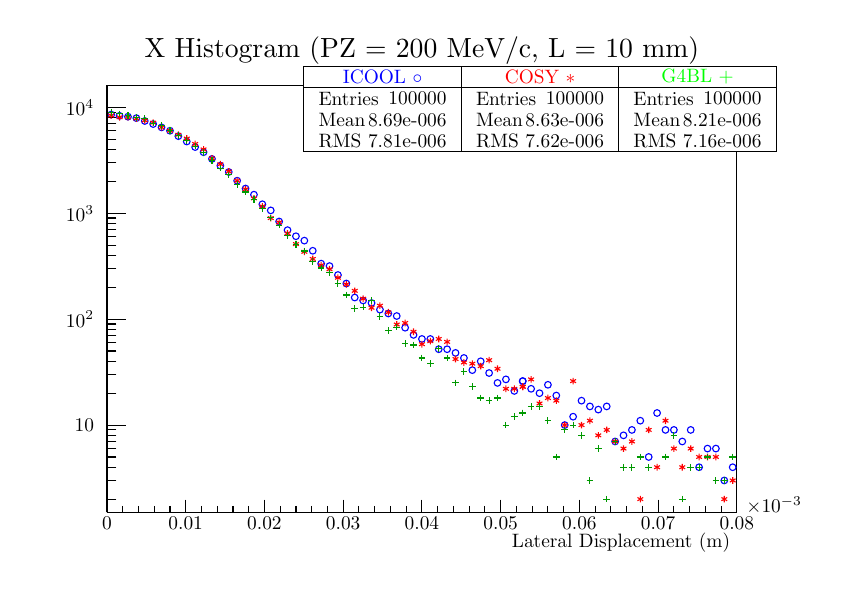
\begin{tikzpicture}
\definecolor{c}{rgb}{1,1,1};
\draw [color=c, fill=c] (0,0) rectangle (20,13.5632);
\draw [color=c, fill=c] (2,1.35632) rectangle (18,12.2069);
\definecolor{c}{rgb}{0,0,0};
\draw [c] (2,1.35632) -- (2,12.2069) -- (18,12.2069) -- (18,1.35632) -- (2,1.35632);
\definecolor{c}{rgb}{1,1,1};
\draw [color=c, fill=c] (2,1.35632) rectangle (18,12.2069);
\definecolor{c}{rgb}{0,0,0};
\draw [c] (2,1.35632) -- (2,12.2069) -- (18,12.2069) -- (18,1.35632) -- (2,1.35632);
\definecolor{c}{rgb}{0,0,1};
\foreach \P in
 {(2.10667,11.4601),(2.32,11.428),(2.53333,11.4057),(2.74667,11.3701),(2.96,11.2967),(3.17333,11.2194),(3.38667,11.1346),(3.6,11.0498),(3.81333,10.9122),(4.02667,10.7755),(4.24,10.635),(4.45333,10.5039),(4.66667,10.3337),(4.88,10.1623),(5.09333,10.00
11),(5.30667,9.78061),(5.52,9.58187),(5.73333,9.42563),(5.94667,9.1825),(6.16,9.02632),(6.37333,8.74419),(6.58667,8.52468),(6.8,8.3696),(7.01333,8.25841),(7.22667,8.00082),(7.44,7.67341),(7.65333,7.61237),(7.86667,7.38521),(8.08,7.16946),(8.29333,6.8
1336),(8.50667,6.73794),(8.72,6.67389),(8.93333,6.50603),(9.14667,6.40694),(9.36,6.34318),(9.57333,6.04637),(9.78667,5.86388),(10,5.7607),(10.2133,5.7607),(10.4267,5.49993),(10.64,5.49993),(10.8533,5.40639),(11.0667,5.27785),(11.28,4.96853),(11.4933,
5.19333),(11.7067,4.89546),(11.92,4.64408),(12.1333,4.73402),(12.3467,4.44033),(12.56,4.68992)}{\draw[mark options={color=c,fill=c},mark size=2.402402pt,mark=o] plot coordinates {\P};}
\foreach \P in
 {(12.56,4.68992),(12.7733,4.4947),(12.9867,4.38332),(13.2,4.59638),(13.4133,4.32338),(13.6267,3.5733),(13.84,3.78636),(14.0533,4.1934),(14.2667,4.04713),(14.48,3.96651),(14.6933,4.04713),(14.9067,3.15649),(15.12,3.31254),(15.3333,3.45018),(15.5467,3
.68468),(15.76,2.76329),(15.9733,3.8799),(16.1867,3.45018),(16.4,3.45018),(16.6133,3.15649),(16.8267,3.45018),(17.04,2.50252),(17.2533,2.97635),(17.4667,2.97635),(17.68,2.16634),(17.8933,2.50252)}{\draw[mark options={color=c,fill=c},mark
 size=2.402402pt,mark=o] plot coordinates {\P};}
\definecolor{c}{rgb}{1,1,1};
\draw [color=c, fill=c] (7,10.5115) rectangle (11,12.6816);
\definecolor{c}{rgb}{0,0,0};
\draw [c] (7,10.5115) -- (11,10.5115);
\draw [c] (11,10.5115) -- (11,12.6816);
\draw [c] (11,12.6816) -- (7,12.6816);
\draw [c] (7,12.6816) -- (7,10.5115);
\draw[color=blue](9,12.4103) node[scale=0.7, rotate=0]{ICOOL $\circ$};
\draw [c] (7,12.1391) -- (11,12.1391);
\draw [anchor= west] (7.2,11.8678) node[scale=0.7, rotate=0]{Entries };
\draw [anchor= east] (10.8,11.8678) node[scale=0.7, rotate=0]{ 100000};
\draw [anchor= west] (7.2,11.3253) node[scale=0.7, rotate=0]{Mean  };
\draw [anchor= east] (10.8,11.3253) node[scale=0.7, rotate=0]{ 8.69e-006};
\draw [anchor= west] (7.2,10.7828) node[scale=0.7, rotate=0]{RMS   };
\draw [anchor= east] (10.8,10.7828) node[scale=0.7, rotate=0]{ 7.81e-006};
\draw [c] (2,1.35632) -- (18,1.35632);
\draw [anchor= east] (18,0.596782) node[scale=0.7, rotate=0]{Lateral Displacement (m)};
\draw [c] (2,1.68184) -- (2,1.35632);
\draw [c] (2.4,1.51908) -- (2.4,1.35632);
\draw [c] (2.8,1.51908) -- (2.8,1.35632);
\draw [c] (3.2,1.51908) -- (3.2,1.35632);
\draw [c] (3.6,1.51908) -- (3.6,1.35632);
\draw [c] (4,1.68184) -- (4,1.35632);
\draw [c] (4.4,1.51908) -- (4.4,1.35632);
\draw [c] (4.8,1.51908) -- (4.8,1.35632);
\draw [c] (5.2,1.51908) -- (5.2,1.35632);
\draw [c] (5.6,1.51908) -- (5.6,1.35632);
\draw [c] (6,1.68184) -- (6,1.35632);
\draw [c] (6.4,1.51908) -- (6.4,1.35632);
\draw [c] (6.8,1.51908) -- (6.8,1.35632);
\draw [c] (7.2,1.51908) -- (7.2,1.35632);
\draw [c] (7.6,1.51908) -- (7.6,1.35632);
\draw [c] (8,1.68184) -- (8,1.35632);
\draw [c] (8.4,1.51908) -- (8.4,1.35632);
\draw [c] (8.8,1.51908) -- (8.8,1.35632);
\draw [c] (9.2,1.51908) -- (9.2,1.35632);
\draw [c] (9.6,1.51908) -- (9.6,1.35632);
\draw [c] (10,1.68184) -- (10,1.35632);
\draw [c] (10.4,1.51908) -- (10.4,1.35632);
\draw [c] (10.8,1.51908) -- (10.8,1.35632);
\draw [c] (11.2,1.51908) -- (11.2,1.35632);
\draw [c] (11.6,1.51908) -- (11.6,1.35632);
\draw [c] (12,1.68184) -- (12,1.35632);
\draw [c] (12.4,1.51908) -- (12.4,1.35632);
\draw [c] (12.8,1.51908) -- (12.8,1.35632);
\draw [c] (13.2,1.51908) -- (13.2,1.35632);
\draw [c] (13.6,1.51908) -- (13.6,1.35632);
\draw [c] (14,1.68184) -- (14,1.35632);
\draw [c] (14.4,1.51908) -- (14.4,1.35632);
\draw [c] (14.8,1.51908) -- (14.8,1.35632);
\draw [c] (15.2,1.51908) -- (15.2,1.35632);
\draw [c] (15.6,1.51908) -- (15.6,1.35632);
\draw [c] (16,1.68184) -- (16,1.35632);
\draw [c] (16.4,1.51908) -- (16.4,1.35632);
\draw [c] (16.8,1.51908) -- (16.8,1.35632);
\draw [c] (17.2,1.51908) -- (17.2,1.35632);
\draw [c] (17.6,1.51908) -- (17.6,1.35632);
\draw [c] (18,1.68184) -- (18,1.35632);
\draw [c] (18,1.68184) -- (18,1.35632);
\draw [anchor=base] (2,0.908736) node[scale=0.7, rotate=0]{0};
\draw [anchor=base] (4,0.908736) node[scale=0.7, rotate=0]{0.01};
\draw [anchor=base] (6,0.908736) node[scale=0.7, rotate=0]{0.02};
\draw [anchor=base] (8,0.908736) node[scale=0.7, rotate=0]{0.03};
\draw [anchor=base] (10,0.908736) node[scale=0.7, rotate=0]{0.04};
\draw [anchor=base] (12,0.908736) node[scale=0.7, rotate=0]{0.05};
\draw [anchor=base] (14,0.908736) node[scale=0.7, rotate=0]{0.06};
\draw [anchor=base] (16,0.908736) node[scale=0.7, rotate=0]{0.07};
\draw [anchor=base] (18,0.908736) node[scale=0.7, rotate=0]{0.08};
\draw [anchor=base west] (18.07,1.35632) node[scale=0.7, rotate=0]{$\times10^{-3}$};
\draw [c] (2,1.35632) -- (2,12.2069);
\draw [c] (2.24,1.69251) -- (2,1.69251);
\draw [c] (2.24,2.16633) -- (2,2.16633);
\draw [c] (2.24,2.50252) -- (2,2.50252);
\draw [c] (2.24,2.76329) -- (2,2.76329);
\draw [c] (2.24,2.97635) -- (2,2.97635);
\draw [c] (2.24,3.15649) -- (2,3.15649);
\draw [c] (2.24,3.31253) -- (2,3.31253);
\draw [c] (2.24,3.45018) -- (2,3.45018);
\draw [c] (2.48,3.5733) -- (2,3.5733);
\draw [anchor= east] (1.844,3.5733) node[scale=0.7, rotate=0]{10};
\draw [c] (2.24,4.38332) -- (2,4.38332);
\draw [c] (2.24,4.85714) -- (2,4.85714);
\draw [c] (2.24,5.19333) -- (2,5.19333);
\draw [c] (2.24,5.4541) -- (2,5.4541);
\draw [c] (2.24,5.66716) -- (2,5.66716);
\draw [c] (2.24,5.8473) -- (2,5.8473);
\draw [c] (2.24,6.00334) -- (2,6.00334);
\draw [c] (2.24,6.14099) -- (2,6.14099);
\draw [c] (2.48,6.26411) -- (2,6.26411);
\draw [anchor= east] (1.844,6.26411) node[scale=0.7, rotate=0]{$10^{2}$};
\draw [c] (2.24,7.07413) -- (2,7.07413);
\draw [c] (2.24,7.54795) -- (2,7.54795);
\draw [c] (2.24,7.88414) -- (2,7.88414);
\draw [c] (2.24,8.14491) -- (2,8.14491);
\draw [c] (2.24,8.35797) -- (2,8.35797);
\draw [c] (2.24,8.53811) -- (2,8.53811);
\draw [c] (2.24,8.69415) -- (2,8.69415);
\draw [c] (2.24,8.8318) -- (2,8.8318);
\draw [c] (2.48,8.95492) -- (2,8.95492);
\draw [anchor= east] (1.844,8.95492) node[scale=0.7, rotate=0]{$10^{3}$};
\draw [c] (2.24,9.76494) -- (2,9.76494);
\draw [c] (2.24,10.2388) -- (2,10.2388);
\draw [c] (2.24,10.575) -- (2,10.575);
\draw [c] (2.24,10.8357) -- (2,10.8357);
\draw [c] (2.24,11.0488) -- (2,11.0488);
\draw [c] (2.24,11.2289) -- (2,11.2289);
\draw [c] (2.24,11.385) -- (2,11.385);
\draw [c] (2.24,11.5226) -- (2,11.5226);
\draw [c] (2.48,11.6457) -- (2,11.6457);
\draw [anchor= east] (1.844,11.6457) node[scale=0.7, rotate=0]{$10^{4}$};
\definecolor{c}{rgb}{1,1,1};
\draw [color=c, fill=c] (7,10.5115) rectangle (11,12.6816);
\definecolor{c}{rgb}{0,0,0};
\draw [c] (7,10.5115) -- (11,10.5115);
\draw [c] (11,10.5115) -- (11,12.6816);
\draw [c] (11,12.6816) -- (7,12.6816);
\draw [c] (7,12.6816) -- (7,10.5115);
\draw[color=blue](9,12.4103) node[scale=0.7, rotate=0]{ICOOL $\circ$};
\draw [c] (7,12.1391) -- (11,12.1391);
\draw [anchor= west] (7.2,11.8678) node[scale=0.7, rotate=0]{Entries };
\draw [anchor= east] (10.8,11.8678) node[scale=0.7, rotate=0]{ 100000};
\draw [anchor= west] (7.2,11.3253) node[scale=0.7, rotate=0]{Mean  };
\draw [anchor= east] (10.8,11.3253) node[scale=0.7, rotate=0]{ 8.69e-006};
\draw [anchor= west] (7.2,10.7828) node[scale=0.7, rotate=0]{RMS   };
\draw [anchor= east] (10.8,10.7828) node[scale=0.7, rotate=0]{ 7.81e-006};
\draw (10,13.0816) node[scale=1, rotate=0]{X Histogram (PZ = 200 MeV/c, L = 10 mm)};
\definecolor{c}{rgb}{1,0,0};
\foreach \P in
 {(2.10667,11.4351),(2.32,11.3914),(2.53333,11.3947),(2.74667,11.3596),(2.96,11.3116),(3.17333,11.2542),(3.38667,11.1362),(3.6,11.0499),(3.81333,10.9469),(4.02667,10.8506),(4.24,10.7129),(4.45333,10.5755),(4.66667,10.3455),(4.88,10.1983),(5.09333,10.
0154),(5.30667,9.7783),(5.52,9.56258),(5.73333,9.33216),(5.94667,9.12837),(6.16,8.8305),(6.37333,8.72159),(6.58667,8.44248),(6.8,8.17034),(7.01333,7.97408),(7.22667,7.79304),(7.44,7.63428),(7.65333,7.53227),(7.86667,7.31604),(8.08,7.14772),(8.29333,6
.98302),(8.50667,6.78377),(8.72,6.55259),(8.93333,6.60613),(9.14667,6.43756),(9.36,6.12793),(9.57333,6.16667),(9.78667,5.9434),(10,5.62754),(10.2133,5.70548),(10.4267,5.7607),(10.64,5.68648),(10.8533,5.25035),(11.0667,5.16375),(11.28,5.13339),(11.493
3,5.07021),(11.7067,5.22219),(11.92,5.00341),(12.1333,4.4947),(12.3467,4.4947),(12.56,4.54664)}{\draw[mark options={color=c,fill=c},mark size=2.402402pt,mark=asterisk] plot coordinates {\P};}
\foreach \P in
 {(12.56,4.54664),(12.7733,4.73402),(12.9867,4.12255),(13.2,4.26019),(13.4133,4.1934),(13.6267,3.5733),(13.84,4.68992),(14.0533,3.5733),(14.2667,3.68468),(14.48,3.31254),(14.6933,3.45018),(14.9067,3.15649),(15.12,2.97635),(15.3333,3.15649),(15.5467,1
.69251),(15.76,3.45018),(15.9733,2.50252),(16.1867,3.68468),(16.4,2.97635),(16.6133,2.50252),(16.8267,2.97635),(17.04,2.76329),(17.2533,2.76329),(17.4667,2.76329),(17.68,1.69251),(17.8933,2.16634)}{\draw[mark options={color=c,fill=c},mark
 size=2.402402pt,mark=asterisk] plot coordinates {\P};}
\definecolor{c}{rgb}{1,1,1};
\draw [color=c, fill=c] (11,10.5115) rectangle (15,12.6816);
\definecolor{c}{rgb}{0,0,0};
\draw [c] (11,10.5115) -- (15,10.5115);
\draw [c] (15,10.5115) -- (15,12.6816);
\draw [c] (15,12.6816) -- (11,12.6816);
\draw [c] (11,12.6816) -- (11,10.5115);
\draw [color=red](13,12.4103) node[scale=0.7, rotate=0]{COSY $*$};
\draw [c] (11,12.1391) -- (15,12.1391);
\draw [anchor= west] (11.2,11.8678) node[scale=0.7, rotate=0]{Entries };
\draw [anchor= east] (14.8,11.8678) node[scale=0.7, rotate=0]{ 100000};
\draw [anchor= west] (11.2,11.3253) node[scale=0.7, rotate=0]{Mean  };
\draw [anchor= east] (14.8,11.3253) node[scale=0.7, rotate=0]{ 8.63e-006};
\draw [anchor= west] (11.2,10.7828) node[scale=0.7, rotate=0]{RMS   };
\draw [anchor= east] (14.8,10.7828) node[scale=0.7, rotate=0]{ 7.62e-006};
\definecolor{c}{rgb}{1,1,1};
\draw [color=c, fill=c] (11,10.5115) rectangle (15,12.6816);
\definecolor{c}{rgb}{0,0,0};
\draw [c] (11,10.5115) -- (15,10.5115);
\draw [c] (15,10.5115) -- (15,12.6816);
\draw [c] (15,12.6816) -- (11,12.6816);
\draw [c] (11,12.6816) -- (11,10.5115);
\draw [color=red](13,12.4103) node[scale=0.7, rotate=0]{COSY $*$};
\draw [c] (11,12.1391) -- (15,12.1391);
\draw [anchor= west] (11.2,11.8678) node[scale=0.7, rotate=0]{Entries };
\draw [anchor= east] (14.8,11.8678) node[scale=0.7, rotate=0]{ 100000};
\draw [anchor= west] (11.2,11.3253) node[scale=0.7, rotate=0]{Mean  };
\draw [anchor= east] (14.8,11.3253) node[scale=0.7, rotate=0]{ 8.63e-006};
\draw [anchor= west] (11.2,10.7828) node[scale=0.7, rotate=0]{RMS   };
\draw [anchor= east] (14.8,10.7828) node[scale=0.7, rotate=0]{ 7.62e-006};
\definecolor{c}{rgb}{0,0.6,0};
\foreach \P in
 {(2.10667,11.5173),(2.32,11.4767),(2.53333,11.4342),(2.74667,11.3931),(2.96,11.3543),(3.17333,11.242),(3.38667,11.1828),(3.6,11.0635),(3.81333,10.9304),(4.02667,10.8018),(4.24,10.6603),(4.45333,10.4952),(4.66667,10.2999),(4.88,10.0991),(5.09333,9.92
877),(5.30667,9.68952),(5.52,9.4939),(5.73333,9.30649),(5.94667,9.07688),(6.16,8.83439),(6.37333,8.65252),(6.58667,8.39062),(6.8,8.15654),(7.01333,7.99552),(7.22667,7.7281),(7.44,7.56343),(7.65333,7.43774),(7.86667,7.16406),(8.08,6.87731),(8.29333,6.
53419),(8.50667,6.57071),(8.72,6.73794),(8.93333,6.33221),(9.14667,5.97376),(9.36,6.06036),(9.57333,5.64752),(9.78667,5.60722),(10,5.27785),(10.2133,5.13339),(10.4267,5.52219),(10.64,5.27785),(10.8533,4.64408),(11.0667,4.93257),(11.28,4.54664),(11.49
33,4.26019),(11.7067,4.1934),(11.92,4.26019),(12.1333,3.5733),(12.3467,3.78636),(12.56,3.8799)}{\draw[mark options={color=c,fill=c},mark size=2.402402pt,mark=+] plot coordinates {\P};}
\foreach \P in
 {(12.56,3.8799),(12.7733,4.04713),(12.9867,4.04713),(13.2,3.68468),(13.4133,2.76329),(13.6267,3.45018),(13.84,3.5733),(14.0533,3.31254),(14.2667,2.16634),(14.48,2.97635),(14.6933,1.69251),(14.9067,3.15649),(15.12,2.50252),(15.3333,2.50252),(15.5467,
2.76329),(15.76,2.50252),(16.1867,2.76329),(16.4,3.31254),(16.6133,1.69251),(16.8267,2.50252),(17.04,2.50252),(17.2533,2.76329),(17.4667,2.16634),(17.68,2.16634),(17.8933,2.76329)}{\draw[mark options={color=c,fill=c},mark size=2.402402pt,mark=+] plot
 coordinates {\P};}
\definecolor{c}{rgb}{1,1,1};
\draw [color=c, fill=c] (15,10.5115) rectangle (19,12.6816);
\definecolor{c}{rgb}{0,0,0};
\draw [c] (15,10.5115) -- (19,10.5115);
\draw [c] (19,10.5115) -- (19,12.6816);
\draw [c] (19,12.6816) -- (15,12.6816);
\draw [c] (15,12.6816) -- (15,10.5115);
\draw [color=green](17,12.4103) node[scale=0.7, rotate=0]{G4BL $+$};
\draw [c] (15,12.1391) -- (19,12.1391);
\draw [anchor= west] (15.2,11.8678) node[scale=0.7, rotate=0]{Entries };
\draw [anchor= east] (18.8,11.8678) node[scale=0.7, rotate=0]{ 100000};
\draw [anchor= west] (15.2,11.3253) node[scale=0.7, rotate=0]{Mean  };
\draw [anchor= east] (18.8,11.3253) node[scale=0.7, rotate=0]{ 8.21e-006};
\draw [anchor= west] (15.2,10.7828) node[scale=0.7, rotate=0]{RMS   };
\draw [anchor= east] (18.8,10.7828) node[scale=0.7, rotate=0]{ 7.16e-006};
\definecolor{c}{rgb}{1,1,1};
\draw [color=c, fill=c] (15,10.5115) rectangle (19,12.6816);
\definecolor{c}{rgb}{0,0,0};
\draw [c] (15,10.5115) -- (19,10.5115);
\draw [c] (19,10.5115) -- (19,12.6816);
\draw [c] (19,12.6816) -- (15,12.6816);
\draw [c] (15,12.6816) -- (15,10.5115);
\draw [color=green](17,12.4103) node[scale=0.7, rotate=0]{G4BL $+$};
\draw [c] (15,12.1391) -- (19,12.1391);
\draw [anchor= west] (15.2,11.8678) node[scale=0.7, rotate=0]{Entries };
\draw [anchor= east] (18.8,11.8678) node[scale=0.7, rotate=0]{ 100000};
\draw [anchor= west] (15.2,11.3253) node[scale=0.7, rotate=0]{Mean  };
\draw [anchor= east] (18.8,11.3253) node[scale=0.7, rotate=0]{ 8.21e-006};
\draw [anchor= west] (15.2,10.7828) node[scale=0.7, rotate=0]{RMS   };
\draw [anchor= east] (18.8,10.7828) node[scale=0.7, rotate=0]{ 7.16e-006};
\end{tikzpicture}
}\\
\frame{    \pgfdeclareplotmark{cross} {
\pgfpathmoveto{\pgfpoint{-0.3\pgfplotmarksize}{\pgfplotmarksize}}
\pgfpathlineto{\pgfpoint{+0.3\pgfplotmarksize}{\pgfplotmarksize}}
\pgfpathlineto{\pgfpoint{+0.3\pgfplotmarksize}{0.3\pgfplotmarksize}}
\pgfpathlineto{\pgfpoint{+1\pgfplotmarksize}{0.3\pgfplotmarksize}}
\pgfpathlineto{\pgfpoint{+1\pgfplotmarksize}{-0.3\pgfplotmarksize}}
\pgfpathlineto{\pgfpoint{+0.3\pgfplotmarksize}{-0.3\pgfplotmarksize}}
\pgfpathlineto{\pgfpoint{+0.3\pgfplotmarksize}{-1.\pgfplotmarksize}}
\pgfpathlineto{\pgfpoint{-0.3\pgfplotmarksize}{-1.\pgfplotmarksize}}
\pgfpathlineto{\pgfpoint{-0.3\pgfplotmarksize}{-0.3\pgfplotmarksize}}
\pgfpathlineto{\pgfpoint{-1.\pgfplotmarksize}{-0.3\pgfplotmarksize}}
\pgfpathlineto{\pgfpoint{-1.\pgfplotmarksize}{0.3\pgfplotmarksize}}
\pgfpathlineto{\pgfpoint{-0.3\pgfplotmarksize}{0.3\pgfplotmarksize}}
\pgfpathclose
\pgfusepathqstroke
}
\pgfdeclareplotmark{cross*} {
\pgfpathmoveto{\pgfpoint{-0.3\pgfplotmarksize}{\pgfplotmarksize}}
\pgfpathlineto{\pgfpoint{+0.3\pgfplotmarksize}{\pgfplotmarksize}}
\pgfpathlineto{\pgfpoint{+0.3\pgfplotmarksize}{0.3\pgfplotmarksize}}
\pgfpathlineto{\pgfpoint{+1\pgfplotmarksize}{0.3\pgfplotmarksize}}
\pgfpathlineto{\pgfpoint{+1\pgfplotmarksize}{-0.3\pgfplotmarksize}}
\pgfpathlineto{\pgfpoint{+0.3\pgfplotmarksize}{-0.3\pgfplotmarksize}}
\pgfpathlineto{\pgfpoint{+0.3\pgfplotmarksize}{-1.\pgfplotmarksize}}
\pgfpathlineto{\pgfpoint{-0.3\pgfplotmarksize}{-1.\pgfplotmarksize}}
\pgfpathlineto{\pgfpoint{-0.3\pgfplotmarksize}{-0.3\pgfplotmarksize}}
\pgfpathlineto{\pgfpoint{-1.\pgfplotmarksize}{-0.3\pgfplotmarksize}}
\pgfpathlineto{\pgfpoint{-1.\pgfplotmarksize}{0.3\pgfplotmarksize}}
\pgfpathlineto{\pgfpoint{-0.3\pgfplotmarksize}{0.3\pgfplotmarksize}}
\pgfpathclose
\pgfusepathqfillstroke
}
\pgfdeclareplotmark{newstar} {
\pgfpathmoveto{\pgfqpoint{0pt}{\pgfplotmarksize}}
\pgfpathlineto{\pgfqpointpolar{44}{0.5\pgfplotmarksize}}
\pgfpathlineto{\pgfqpointpolar{18}{\pgfplotmarksize}}
\pgfpathlineto{\pgfqpointpolar{-20}{0.5\pgfplotmarksize}}
\pgfpathlineto{\pgfqpointpolar{-54}{\pgfplotmarksize}}
\pgfpathlineto{\pgfqpointpolar{-90}{0.5\pgfplotmarksize}}
\pgfpathlineto{\pgfqpointpolar{234}{\pgfplotmarksize}}
\pgfpathlineto{\pgfqpointpolar{198}{0.5\pgfplotmarksize}}
\pgfpathlineto{\pgfqpointpolar{162}{\pgfplotmarksize}}
\pgfpathlineto{\pgfqpointpolar{134}{0.5\pgfplotmarksize}}
\pgfpathclose
\pgfusepathqstroke
}
\pgfdeclareplotmark{newstar*} {
\pgfpathmoveto{\pgfqpoint{0pt}{\pgfplotmarksize}}
\pgfpathlineto{\pgfqpointpolar{44}{0.5\pgfplotmarksize}}
\pgfpathlineto{\pgfqpointpolar{18}{\pgfplotmarksize}}
\pgfpathlineto{\pgfqpointpolar{-20}{0.5\pgfplotmarksize}}
\pgfpathlineto{\pgfqpointpolar{-54}{\pgfplotmarksize}}
\pgfpathlineto{\pgfqpointpolar{-90}{0.5\pgfplotmarksize}}
\pgfpathlineto{\pgfqpointpolar{234}{\pgfplotmarksize}}
\pgfpathlineto{\pgfqpointpolar{198}{0.5\pgfplotmarksize}}
\pgfpathlineto{\pgfqpointpolar{162}{\pgfplotmarksize}}
\pgfpathlineto{\pgfqpointpolar{134}{0.5\pgfplotmarksize}}
\pgfpathclose
\pgfusepathqfillstroke
}
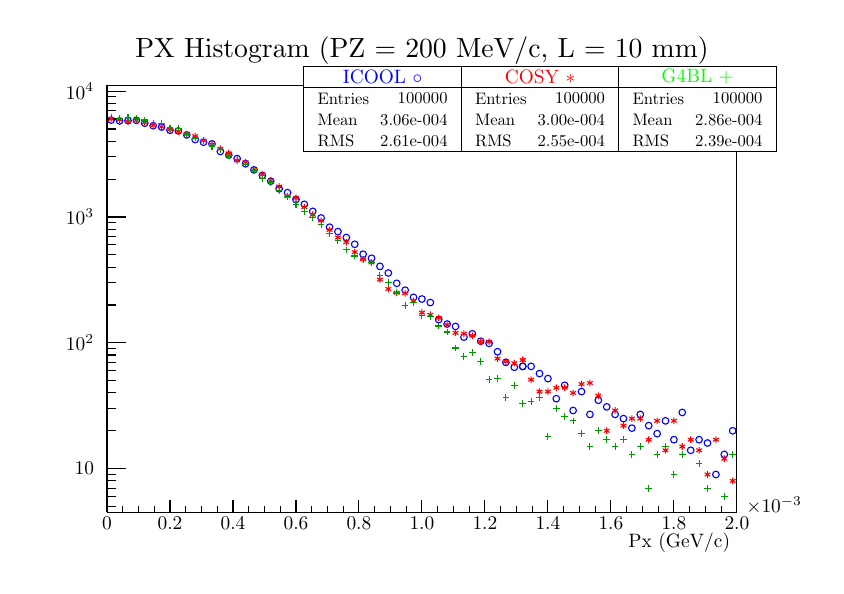
\begin{tikzpicture}
\definecolor{c}{rgb}{1,1,1};
\draw [color=c, fill=c] (0,0) rectangle (20,13.5632);
\draw [color=c, fill=c] (2,1.35632) rectangle (18,12.2069);
\definecolor{c}{rgb}{0,0,0};
\draw [c] (2,1.35632) -- (2,12.2069) -- (18,12.2069) -- (18,1.35632) -- (2,1.35632);
\definecolor{c}{rgb}{1,1,1};
\draw [color=c, fill=c] (2,1.35632) rectangle (18,12.2069);
\definecolor{c}{rgb}{0,0,0};
\draw [c] (2,1.35632) -- (2,12.2069) -- (18,12.2069) -- (18,1.35632) -- (2,1.35632);
\definecolor{c}{rgb}{0,0,1};
\foreach \P in
 {(2.10667,11.3196),(2.32,11.2991),(2.53333,11.3073),(2.74667,11.3139),(2.96,11.2412),(3.17333,11.1778),(3.38667,11.1435),(3.6,11.0615),(3.81333,11.0449),(4.02667,10.9448),(4.24,10.8258),(4.45333,10.7582),(4.66667,10.7154),(4.88,10.5229),(5.09333,10.
4316),(5.30667,10.342),(5.52,10.2105),(5.73333,10.0553),(5.94667,9.91333),(6.16,9.76755),(6.37333,9.57429),(6.58667,9.47726),(6.8,9.30211),(7.01333,9.18093),(7.22667,9.00134),(7.44,8.83373),(7.65333,8.60025),(7.86667,8.48702),(8.08,8.33771),(8.29333,
8.16581),(8.50667,7.91313),(8.72,7.81066),(8.93333,7.60399),(9.14667,7.4366),(9.36,7.17337),(9.57333,6.99927),(9.78667,6.81841),(10,6.7755),(10.2133,6.68547),(10.4267,6.25243),(10.64,6.13902),(10.8533,6.07865),(11.0667,5.80687),(11.28,5.89178),(11.49
33,5.70301),(11.7067,5.64802),(11.92,5.43633),(12.1333,5.16675),(12.3467,5.04233),(12.56,5.06386)}{\draw[mark options={color=c,fill=c},mark size=2.402402pt,mark=o] plot coordinates {\P};}
\foreach \P in
 {(12.56,5.06386),(12.7733,5.06386),(12.9867,4.88151),(13.2,4.75404),(13.4133,4.24348),(13.6267,4.58382),(13.84,3.94327),(14.0533,4.42405),(14.2667,3.84405),(14.48,4.20437),(14.6933,4.03587),(14.9067,3.84405),(15.12,3.7372),(15.3333,3.49512),(15.5467
,3.84405),(15.76,3.55971),(15.9733,3.35616),(16.1867,3.68052),(16.4,3.20173),(16.6133,3.89455),(16.8267,2.93216),(17.04,3.20173),(17.2533,3.11756),(17.4667,2.31871),(17.68,2.82927),(17.8933,3.42738)}{\draw[mark options={color=c,fill=c},mark
 size=2.402402pt,mark=o] plot coordinates {\P};}
\definecolor{c}{rgb}{1,1,1};
\draw [color=c, fill=c] (7,10.5115) rectangle (11,12.6816);
\definecolor{c}{rgb}{0,0,0};
\draw [c] (7,10.5115) -- (11,10.5115);
\draw [c] (11,10.5115) -- (11,12.6816);
\draw [c] (11,12.6816) -- (7,12.6816);
\draw [c] (7,12.6816) -- (7,10.5115);
\draw[color=blue](9,12.4103) node[scale=0.7, rotate=0]{ICOOL $\circ$};
\draw [c] (7,12.1391) -- (11,12.1391);
\draw [anchor= west] (7.2,11.8678) node[scale=0.6, rotate=0]{Entries };
\draw [anchor= east] (10.8,11.8678) node[scale=0.6, rotate=0]{ 100000};
\draw [anchor= west] (7.2,11.3253) node[scale=0.6, rotate=0]{Mean  };
\draw [anchor= east] (10.8,11.3253) node[scale=0.6, rotate=0]{ 3.06e-004};
\draw [anchor= west] (7.2,10.7828) node[scale=0.6, rotate=0]{RMS   };
\draw [anchor= east] (10.8,10.7828) node[scale=0.6, rotate=0]{ 2.61e-004};
\draw [c] (2,1.35632) -- (18,1.35632);
\draw [anchor= east] (18,0.596782) node[scale=0.7, rotate=0]{Px (GeV/c)};
\draw [c] (2,1.68184) -- (2,1.35632);
\draw [c] (2.4,1.51908) -- (2.4,1.35632);
\draw [c] (2.8,1.51908) -- (2.8,1.35632);
\draw [c] (3.2,1.51908) -- (3.2,1.35632);
\draw [c] (3.6,1.68184) -- (3.6,1.35632);
\draw [c] (4,1.51908) -- (4,1.35632);
\draw [c] (4.4,1.51908) -- (4.4,1.35632);
\draw [c] (4.8,1.51908) -- (4.8,1.35632);
\draw [c] (5.2,1.68184) -- (5.2,1.35632);
\draw [c] (5.6,1.51908) -- (5.6,1.35632);
\draw [c] (6,1.51908) -- (6,1.35632);
\draw [c] (6.4,1.51908) -- (6.4,1.35632);
\draw [c] (6.8,1.68184) -- (6.8,1.35632);
\draw [c] (7.2,1.51908) -- (7.2,1.35632);
\draw [c] (7.6,1.51908) -- (7.6,1.35632);
\draw [c] (8,1.51908) -- (8,1.35632);
\draw [c] (8.4,1.68184) -- (8.4,1.35632);
\draw [c] (8.8,1.51908) -- (8.8,1.35632);
\draw [c] (9.2,1.51908) -- (9.2,1.35632);
\draw [c] (9.6,1.51908) -- (9.6,1.35632);
\draw [c] (10,1.68184) -- (10,1.35632);
\draw [c] (10.4,1.51908) -- (10.4,1.35632);
\draw [c] (10.8,1.51908) -- (10.8,1.35632);
\draw [c] (11.2,1.51908) -- (11.2,1.35632);
\draw [c] (11.6,1.68184) -- (11.6,1.35632);
\draw [c] (12,1.51908) -- (12,1.35632);
\draw [c] (12.4,1.51908) -- (12.4,1.35632);
\draw [c] (12.8,1.51908) -- (12.8,1.35632);
\draw [c] (13.2,1.68184) -- (13.2,1.35632);
\draw [c] (13.6,1.51908) -- (13.6,1.35632);
\draw [c] (14,1.51908) -- (14,1.35632);
\draw [c] (14.4,1.51908) -- (14.4,1.35632);
\draw [c] (14.8,1.68184) -- (14.8,1.35632);
\draw [c] (15.2,1.51908) -- (15.2,1.35632);
\draw [c] (15.6,1.51908) -- (15.6,1.35632);
\draw [c] (16,1.51908) -- (16,1.35632);
\draw [c] (16.4,1.68184) -- (16.4,1.35632);
\draw [c] (16.8,1.51908) -- (16.8,1.35632);
\draw [c] (17.2,1.51908) -- (17.2,1.35632);
\draw [c] (17.6,1.51908) -- (17.6,1.35632);
\draw [c] (18,1.68184) -- (18,1.35632);
\draw [anchor=base] (2,0.908736) node[scale=0.7, rotate=0]{0};
\draw [anchor=base] (3.6,0.908736) node[scale=0.7, rotate=0]{0.2};
\draw [anchor=base] (5.2,0.908736) node[scale=0.7, rotate=0]{0.4};
\draw [anchor=base] (6.8,0.908736) node[scale=0.7, rotate=0]{0.6};
\draw [anchor=base] (8.4,0.908736) node[scale=0.7, rotate=0]{0.8};
\draw [anchor=base] (10,0.908736) node[scale=0.7, rotate=0]{1.0};
\draw [anchor=base] (11.6,0.908736) node[scale=0.7, rotate=0]{1.2};
\draw [anchor=base] (13.2,0.908736) node[scale=0.7, rotate=0]{1.4};
\draw [anchor=base] (14.8,0.908736) node[scale=0.7, rotate=0]{1.6};
\draw [anchor=base] (16.4,0.908736) node[scale=0.7, rotate=0]{1.8};
\draw [anchor=base] (18,0.908736) node[scale=0.7, rotate=0]{2.0};
\draw [anchor=base west] (18.07,1.35632) node[scale=0.7, rotate=0]{$\times10^{-3}$};
\draw [c] (2,1.35632) -- (2,12.2069);
\draw [c] (2.24,1.5026) -- (2,1.5026);
\draw [c] (2.24,1.75575) -- (2,1.75575);
\draw [c] (2.24,1.96977) -- (2,1.96977);
\draw [c] (2.24,2.15517) -- (2,2.15517);
\draw [c] (2.24,2.31871) -- (2,2.31871);
\draw [c] (2.48,2.46499) -- (2,2.46499);
\draw [anchor= east] (1.844,2.46499) node[scale=0.7, rotate=0]{10};
\draw [c] (2.24,3.42738) -- (2,3.42738);
\draw [c] (2.24,3.99034) -- (2,3.99034);
\draw [c] (2.24,4.38976) -- (2,4.38976);
\draw [c] (2.24,4.69958) -- (2,4.69958);
\draw [c] (2.24,4.95272) -- (2,4.95272);
\draw [c] (2.24,5.16675) -- (2,5.16675);
\draw [c] (2.24,5.35215) -- (2,5.35215);
\draw [c] (2.24,5.51569) -- (2,5.51569);
\draw [c] (2.48,5.66197) -- (2,5.66197);
\draw [anchor= east] (1.844,5.66197) node[scale=0.7, rotate=0]{$10^{2}$};
\draw [c] (2.24,6.62436) -- (2,6.62436);
\draw [c] (2.24,7.18732) -- (2,7.18732);
\draw [c] (2.24,7.58674) -- (2,7.58674);
\draw [c] (2.24,7.89656) -- (2,7.89656);
\draw [c] (2.24,8.1497) -- (2,8.1497);
\draw [c] (2.24,8.36373) -- (2,8.36373);
\draw [c] (2.24,8.54913) -- (2,8.54913);
\draw [c] (2.24,8.71266) -- (2,8.71266);
\draw [c] (2.48,8.85895) -- (2,8.85895);
\draw [anchor= east] (1.844,8.85895) node[scale=0.7, rotate=0]{$10^{3}$};
\draw [c] (2.24,9.82134) -- (2,9.82134);
\draw [c] (2.24,10.3843) -- (2,10.3843);
\draw [c] (2.24,10.7837) -- (2,10.7837);
\draw [c] (2.24,11.0935) -- (2,11.0935);
\draw [c] (2.24,11.3467) -- (2,11.3467);
\draw [c] (2.24,11.5607) -- (2,11.5607);
\draw [c] (2.24,11.7461) -- (2,11.7461);
\draw [c] (2.24,11.9096) -- (2,11.9096);
\draw [c] (2.48,12.0559) -- (2,12.0559);
\draw [anchor= east] (1.844,12.0559) node[scale=0.7, rotate=0]{$10^{4}$};
\definecolor{c}{rgb}{1,1,1};
\draw [color=c, fill=c] (7,10.5115) rectangle (11,12.6816);
\definecolor{c}{rgb}{0,0,0};
\draw [c] (7,10.5115) -- (11,10.5115);
\draw [c] (11,10.5115) -- (11,12.6816);
\draw [c] (11,12.6816) -- (7,12.6816);
\draw [c] (7,12.6816) -- (7,10.5115);
\draw[color=blue](9,12.4103) node[scale=0.7, rotate=0]{ICOOL $\circ$};
\draw [c] (7,12.1391) -- (11,12.1391);
\draw [anchor= west] (7.2,11.8678) node[scale=0.6, rotate=0]{Entries };
\draw [anchor= east] (10.8,11.8678) node[scale=0.6, rotate=0]{ 100000};
\draw [anchor= west] (7.2,11.3253) node[scale=0.6, rotate=0]{Mean  };
\draw [anchor= east] (10.8,11.3253) node[scale=0.6, rotate=0]{ 3.06e-004};
\draw [anchor= west] (7.2,10.7828) node[scale=0.6, rotate=0]{RMS   };
\draw [anchor= east] (10.8,10.7828) node[scale=0.6, rotate=0]{ 2.61e-004};
\draw (10,13.0816) node[scale=1, rotate=0]{PX Histogram (PZ = 200 MeV/c, L = 10 mm)};
\definecolor{c}{rgb}{1,0,0};
\foreach \P in
 {(2.10667,11.3478),(2.32,11.328),(2.53333,11.289),(2.74667,11.3139),(2.96,11.2618),(3.17333,11.1888),(3.38667,11.1485),(3.6,11.0824),(3.81333,11.0314),(4.02667,10.9605),(4.24,10.9123),(4.45333,10.8003),(4.66667,10.7022),(4.88,10.5944),(5.09333,10.47
43),(5.30667,10.2944),(5.52,10.2513),(5.73333,10.0511),(5.94667,9.93844),(6.16,9.77762),(6.37333,9.63197),(6.58667,9.38533),(6.8,9.3419),(7.01333,9.10746),(7.22667,8.91607),(7.44,8.76564),(7.65333,8.52991),(7.86667,8.33771),(8.08,8.21745),(8.29333,7.
96431),(8.50667,7.7808),(8.72,7.70321),(8.93333,7.26822),(9.14667,7.03071),(9.36,6.93418),(9.57333,6.92303),(9.78667,6.72477),(10,6.431),(10.2133,6.37399),(10.4267,6.29708),(10.64,6.11919),(10.8533,5.91511),(11.0667,5.89178),(11.28,5.8439),(11.4933,5
.68947),(11.7067,5.68947),(11.92,5.26255),(12.1333,5.18645),(12.3467,5.14678),(12.56,5.22502)}{\draw[mark options={color=c,fill=c},mark size=2.402402pt,mark=asterisk] plot coordinates {\P};}
\foreach \P in
 {(12.56,5.22502),(12.7733,4.72708),(12.9867,4.42405),(13.2,4.42405),(13.4133,4.5221),(13.6267,4.5221),(13.84,4.38977),(14.0533,4.61368),(14.2667,4.64291),(14.48,4.31855),(14.6933,3.42738),(14.9067,3.94327),(15.12,3.55971),(15.3333,3.7372),(15.5467,3
.7372),(15.76,3.20173),(15.9733,3.68052),(16.1867,2.93216),(16.4,3.68052),(16.6133,3.02795),(16.8267,3.20173),(17.04,2.93216),(17.2533,2.31871),(17.4667,3.20173),(17.68,2.71813),(17.8933,2.15517)}{\draw[mark options={color=c,fill=c},mark
 size=2.402402pt,mark=asterisk] plot coordinates {\P};}
\definecolor{c}{rgb}{1,1,1};
\draw [color=c, fill=c] (11,10.5115) rectangle (15,12.6816);
\definecolor{c}{rgb}{0,0,0};
\draw [c] (11,10.5115) -- (15,10.5115);
\draw [c] (15,10.5115) -- (15,12.6816);
\draw [c] (15,12.6816) -- (11,12.6816);
\draw [c] (11,12.6816) -- (11,10.5115);
\draw [color=red](13,12.4103) node[scale=0.7, rotate=0]{COSY $*$};
\draw [c] (11,12.1391) -- (15,12.1391);
\draw [anchor= west] (11.2,11.8678) node[scale=0.6, rotate=0]{Entries };
\draw [anchor= east] (14.8,11.8678) node[scale=0.6, rotate=0]{ 100000};
\draw [anchor= west] (11.2,11.3253) node[scale=0.6, rotate=0]{Mean  };
\draw [anchor= east] (14.8,11.3253) node[scale=0.6, rotate=0]{ 3.00e-004};
\draw [anchor= west] (11.2,10.7828) node[scale=0.6, rotate=0]{RMS   };
\draw [anchor= east] (14.8,10.7828) node[scale=0.6, rotate=0]{ 2.55e-004};
\definecolor{c}{rgb}{1,1,1};
\draw [color=c, fill=c] (11,10.5115) rectangle (15,12.6816);
\definecolor{c}{rgb}{0,0,0};
\draw [c] (11,10.5115) -- (15,10.5115);
\draw [c] (15,10.5115) -- (15,12.6816);
\draw [c] (15,12.6816) -- (11,12.6816);
\draw [c] (11,12.6816) -- (11,10.5115);
\draw [color=red](13,12.4103) node[scale=0.7, rotate=0]{COSY $*$};
\draw [c] (11,12.1391) -- (15,12.1391);
\draw [anchor= west] (11.2,11.8678) node[scale=0.6, rotate=0]{Entries };
\draw [anchor= east] (14.8,11.8678) node[scale=0.6, rotate=0]{ 100000};
\draw [anchor= west] (11.2,11.3253) node[scale=0.6, rotate=0]{Mean  };
\draw [anchor= east] (14.8,11.3253) node[scale=0.6, rotate=0]{ 3.00e-004};
\draw [anchor= west] (11.2,10.7828) node[scale=0.6, rotate=0]{RMS   };
\draw [anchor= east] (14.8,10.7828) node[scale=0.6, rotate=0]{ 2.55e-004};
\definecolor{c}{rgb}{0,0.6,0};
\foreach \P in
 {(2.10667,11.3965),(2.32,11.3708),(2.53333,11.3857),(2.74667,11.3705),(2.96,11.3215),(3.17333,11.2422),(3.38667,11.2379),(3.6,11.1221),(3.81333,11.1041),(4.02667,10.9537),(4.24,10.8659),(4.45333,10.7862),(4.66667,10.6513),(4.88,10.5617),(5.09333,10.
4068),(5.30667,10.3204),(5.52,10.1856),(5.73333,10.0417),(5.94667,9.83927),(6.16,9.74132),(6.37333,9.52017),(6.58667,9.38058),(6.8,9.16877),(7.01333,8.9938),(7.22667,8.85339),(7.44,8.67037),(7.65333,8.44464),(7.86667,8.26936),(8.08,8.02384),(8.29333,
7.86852),(8.50667,7.77171),(8.72,7.69681),(8.93333,7.36518),(9.14667,7.18732),(9.36,6.92861),(9.57333,6.6174),(9.78667,6.68547),(10,6.35726),(10.2133,6.33179),(10.4267,6.08889),(10.64,5.93806),(10.8533,5.53103),(11.0667,5.317),(11.28,5.4199),(11.4933
,5.18645),(11.7067,4.72708),(11.92,4.75404),(12.1333,4.28152),(12.3467,4.58382),(12.56,4.12267)}{\draw[mark options={color=c,fill=c},mark size=2.402402pt,mark=+] plot coordinates {\P};}
\foreach \P in
 {(12.56,4.12267),(12.7733,4.16412),(12.9867,4.28152),(13.2,3.28109),(13.4133,3.99034),(13.6267,3.79166),(13.84,3.68052),(14.0533,3.35616),(14.2667,3.02795),(14.48,3.42738),(14.6933,3.20173),(14.9067,3.02795),(15.12,3.20173),(15.3333,2.82927),(15.546
7,3.02795),(15.76,1.96978),(15.9733,2.82927),(16.1867,3.02795),(16.4,2.31871),(16.6133,2.82927),(17.04,2.59733),(17.2533,1.96978),(17.68,1.75575),(17.8933,2.82927)}{\draw[mark options={color=c,fill=c},mark size=2.402402pt,mark=+] plot coordinates
 {\P};}
\definecolor{c}{rgb}{1,1,1};
\draw [color=c, fill=c] (15,10.5115) rectangle (19,12.6816);
\definecolor{c}{rgb}{0,0,0};
\draw [c] (15,10.5115) -- (19,10.5115);
\draw [c] (19,10.5115) -- (19,12.6816);
\draw [c] (19,12.6816) -- (15,12.6816);
\draw [c] (15,12.6816) -- (15,10.5115);
\draw [color=green](17,12.4103) node[scale=0.7, rotate=0]{G4BL $+$};
\draw [c] (15,12.1391) -- (19,12.1391);
\draw [anchor= west] (15.2,11.8678) node[scale=0.6, rotate=0]{Entries };
\draw [anchor= east] (18.8,11.8678) node[scale=0.6, rotate=0]{ 100000};
\draw [anchor= west] (15.2,11.3253) node[scale=0.6, rotate=0]{Mean  };
\draw [anchor= east] (18.8,11.3253) node[scale=0.6, rotate=0]{ 2.86e-004};
\draw [anchor= west] (15.2,10.7828) node[scale=0.6, rotate=0]{RMS   };
\draw [anchor= east] (18.8,10.7828) node[scale=0.6, rotate=0]{ 2.39e-004};
\definecolor{c}{rgb}{1,1,1};
\draw [color=c, fill=c] (15,10.5115) rectangle (19,12.6816);
\definecolor{c}{rgb}{0,0,0};
\draw [c] (15,10.5115) -- (19,10.5115);
\draw [c] (19,10.5115) -- (19,12.6816);
\draw [c] (19,12.6816) -- (15,12.6816);
\draw [c] (15,12.6816) -- (15,10.5115);
\draw [color=green](17,12.4103) node[scale=0.7, rotate=0]{G4BL $+$};
\draw [c] (15,12.1391) -- (19,12.1391);
\draw [anchor= west] (15.2,11.8678) node[scale=0.6, rotate=0]{Entries };
\draw [anchor= east] (18.8,11.8678) node[scale=0.6, rotate=0]{ 100000};
\draw [anchor= west] (15.2,11.3253) node[scale=0.6, rotate=0]{Mean  };
\draw [anchor= east] (18.8,11.3253) node[scale=0.6, rotate=0]{ 2.86e-004};
\draw [anchor= west] (15.2,10.7828) node[scale=0.6, rotate=0]{RMS   };
\draw [anchor= east] (18.8,10.7828) node[scale=0.6, rotate=0]{ 2.39e-004};
\end{tikzpicture}
}\\
\frame{\pgfdeclareplotmark{cross} {
\pgfpathmoveto{\pgfpoint{-0.3\pgfplotmarksize}{\pgfplotmarksize}}
\pgfpathlineto{\pgfpoint{+0.3\pgfplotmarksize}{\pgfplotmarksize}}
\pgfpathlineto{\pgfpoint{+0.3\pgfplotmarksize}{0.3\pgfplotmarksize}}
\pgfpathlineto{\pgfpoint{+1\pgfplotmarksize}{0.3\pgfplotmarksize}}
\pgfpathlineto{\pgfpoint{+1\pgfplotmarksize}{-0.3\pgfplotmarksize}}
\pgfpathlineto{\pgfpoint{+0.3\pgfplotmarksize}{-0.3\pgfplotmarksize}}
\pgfpathlineto{\pgfpoint{+0.3\pgfplotmarksize}{-1.\pgfplotmarksize}}
\pgfpathlineto{\pgfpoint{-0.3\pgfplotmarksize}{-1.\pgfplotmarksize}}
\pgfpathlineto{\pgfpoint{-0.3\pgfplotmarksize}{-0.3\pgfplotmarksize}}
\pgfpathlineto{\pgfpoint{-1.\pgfplotmarksize}{-0.3\pgfplotmarksize}}
\pgfpathlineto{\pgfpoint{-1.\pgfplotmarksize}{0.3\pgfplotmarksize}}
\pgfpathlineto{\pgfpoint{-0.3\pgfplotmarksize}{0.3\pgfplotmarksize}}
\pgfpathclose
\pgfusepathqstroke
}
\pgfdeclareplotmark{cross*} {
\pgfpathmoveto{\pgfpoint{-0.3\pgfplotmarksize}{\pgfplotmarksize}}
\pgfpathlineto{\pgfpoint{+0.3\pgfplotmarksize}{\pgfplotmarksize}}
\pgfpathlineto{\pgfpoint{+0.3\pgfplotmarksize}{0.3\pgfplotmarksize}}
\pgfpathlineto{\pgfpoint{+1\pgfplotmarksize}{0.3\pgfplotmarksize}}
\pgfpathlineto{\pgfpoint{+1\pgfplotmarksize}{-0.3\pgfplotmarksize}}
\pgfpathlineto{\pgfpoint{+0.3\pgfplotmarksize}{-0.3\pgfplotmarksize}}
\pgfpathlineto{\pgfpoint{+0.3\pgfplotmarksize}{-1.\pgfplotmarksize}}
\pgfpathlineto{\pgfpoint{-0.3\pgfplotmarksize}{-1.\pgfplotmarksize}}
\pgfpathlineto{\pgfpoint{-0.3\pgfplotmarksize}{-0.3\pgfplotmarksize}}
\pgfpathlineto{\pgfpoint{-1.\pgfplotmarksize}{-0.3\pgfplotmarksize}}
\pgfpathlineto{\pgfpoint{-1.\pgfplotmarksize}{0.3\pgfplotmarksize}}
\pgfpathlineto{\pgfpoint{-0.3\pgfplotmarksize}{0.3\pgfplotmarksize}}
\pgfpathclose
\pgfusepathqfillstroke
}
\pgfdeclareplotmark{newstar} {
\pgfpathmoveto{\pgfqpoint{0pt}{\pgfplotmarksize}}
\pgfpathlineto{\pgfqpointpolar{44}{0.5\pgfplotmarksize}}
\pgfpathlineto{\pgfqpointpolar{18}{\pgfplotmarksize}}
\pgfpathlineto{\pgfqpointpolar{-20}{0.5\pgfplotmarksize}}
\pgfpathlineto{\pgfqpointpolar{-54}{\pgfplotmarksize}}
\pgfpathlineto{\pgfqpointpolar{-90}{0.5\pgfplotmarksize}}
\pgfpathlineto{\pgfqpointpolar{234}{\pgfplotmarksize}}
\pgfpathlineto{\pgfqpointpolar{198}{0.5\pgfplotmarksize}}
\pgfpathlineto{\pgfqpointpolar{162}{\pgfplotmarksize}}
\pgfpathlineto{\pgfqpointpolar{134}{0.5\pgfplotmarksize}}
\pgfpathclose
\pgfusepathqstroke
}
\pgfdeclareplotmark{newstar*} {
\pgfpathmoveto{\pgfqpoint{0pt}{\pgfplotmarksize}}
\pgfpathlineto{\pgfqpointpolar{44}{0.5\pgfplotmarksize}}
\pgfpathlineto{\pgfqpointpolar{18}{\pgfplotmarksize}}
\pgfpathlineto{\pgfqpointpolar{-20}{0.5\pgfplotmarksize}}
\pgfpathlineto{\pgfqpointpolar{-54}{\pgfplotmarksize}}
\pgfpathlineto{\pgfqpointpolar{-90}{0.5\pgfplotmarksize}}
\pgfpathlineto{\pgfqpointpolar{234}{\pgfplotmarksize}}
\pgfpathlineto{\pgfqpointpolar{198}{0.5\pgfplotmarksize}}
\pgfpathlineto{\pgfqpointpolar{162}{\pgfplotmarksize}}
\pgfpathlineto{\pgfqpointpolar{134}{0.5\pgfplotmarksize}}
\pgfpathclose
\pgfusepathqfillstroke
}
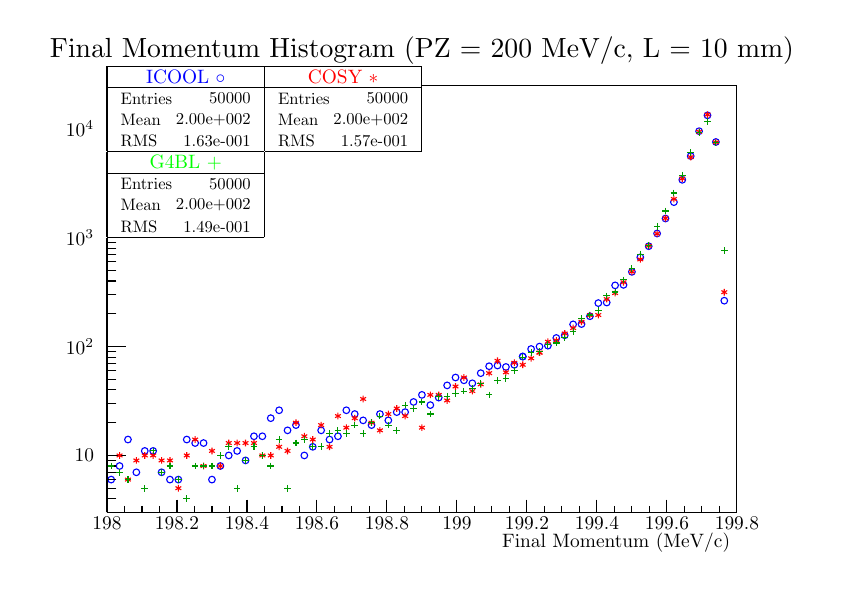
\begin{tikzpicture}
\definecolor{c}{rgb}{1,1,1};
\draw [color=c, fill=c] (0,0) rectangle (20,13.5632);
\draw [color=c, fill=c] (2,1.35632) rectangle (18,12.2069);
\definecolor{c}{rgb}{0,0,0};
\draw [c] (2,1.35632) -- (2,12.2069) -- (18,12.2069) -- (18,1.35632) -- (2,1.35632);
\definecolor{c}{rgb}{1,1,1};
\draw [color=c, fill=c] (2,1.35632) rectangle (18,12.2069);
\definecolor{c}{rgb}{0,0,0};
\draw [c] (2,1.35632) -- (2,12.2069) -- (18,12.2069) -- (18,1.35632) -- (2,1.35632);
\definecolor{c}{rgb}{0,0,1};
\foreach \P in
 {(2.10667,2.18864),(2.32,2.53408),(2.53333,3.20605),(2.74667,2.37374),(2.96,2.91647),(3.17333,2.91647),(3.38667,2.37374),(3.6,2.18864),(3.81333,2.18864),(4.02667,3.20605),(4.24,3.11707),(4.45333,3.11707),(4.66667,2.18864),(4.88,2.53408),(5.09333,2.8
0203),(5.30667,2.91647),(5.52,2.67551),(5.73333,3.2889),(5.94667,3.2889),(6.16,3.74879),(6.37333,3.94938),(6.58667,3.43919),(6.8,3.57275),(7.01333,2.80203),(7.22667,3.02095),(7.44,3.43919),(7.65333,3.20605),(7.86667,3.2889),(8.08,3.94938),(8.29333,3.
85327),(8.50667,3.69293),(8.72,3.57275),(8.93333,3.85327),(9.14667,3.69293),(9.36,3.90229),(9.57333,3.90229),(9.78667,4.16059),(10,4.34014),(10.2133,4.08051),(10.4267,4.27151),(10.64,4.5811),(10.8533,4.7817),(11.0667,4.71034),(11.28,4.63448),(11.4933
,4.89194),(11.7067,5.06798),(11.92,5.08603),(12.1333,5.04964),(12.3467,5.10382),(12.56,5.31389)}{\draw[mark options={color=c,fill=c},mark size=2.402402pt,mark=o] plot coordinates {\P};}
\foreach \P in
 {(12.56,5.31389),(12.7733,5.50533),(12.9867,5.56692),(13.2,5.5907),(13.4133,5.78585),(13.6267,5.85393),(13.84,6.13129),(14.0533,6.13877),(14.2667,6.33764),(14.48,6.67197),(14.6933,6.68624),(14.9067,7.1216),(15.12,7.13469),(15.3333,7.46539),(15.5467,
7.83469),(15.76,8.11672),(15.9733,8.43969),(16.1867,8.81949),(16.4,9.23579),(16.6133,9.80271),(16.8267,10.406),(17.04,11.0381),(17.2533,11.4395),(17.4667,10.7637),(17.68,6.73261)}{\draw[mark options={color=c,fill=c},mark size=2.402402pt,mark=o] plot
 coordinates {\P};}
\definecolor{c}{rgb}{1,1,1};
\draw [color=c, fill=c] (2,10.5115) rectangle (6,12.6816);
\definecolor{c}{rgb}{0,0,0};
\draw [c] (2,10.5115) -- (6,10.5115);
\draw [c] (6,10.5115) -- (6,12.6816);
\draw [c] (6,12.6816) -- (2,12.6816);
\draw [c] (2,12.6816) -- (2,10.5115);
\draw[color=blue](4,12.4103) node[scale=0.7, rotate=0]{ICOOL $\circ$};
\draw [c] (2,12.1391) -- (6,12.1391);
\draw [anchor= west] (2.2,11.8678) node[scale=0.6, rotate=0]{Entries };
\draw [anchor= east] (5.8,11.8678) node[scale=0.6, rotate=0]{ 50000};
\draw [anchor= west] (2.2,11.3253) node[scale=0.6, rotate=0]{Mean  };
\draw [anchor= east] (5.8,11.3253) node[scale=0.6, rotate=0]{ 2.00e+002};
\draw [anchor= west] (2.2,10.7828) node[scale=0.6, rotate=0]{RMS   };
\draw [anchor= east] (5.8,10.7828) node[scale=0.6, rotate=0]{ 1.63e-001};
\draw [c] (2,1.35632) -- (18,1.35632);
\draw [anchor= east] (18,0.596782) node[scale=0.7, rotate=0]{Final Momentum (MeV/c)};
\draw [c] (2,1.68184) -- (2,1.35632);
\draw [c] (2.44444,1.51908) -- (2.44444,1.35632);
\draw [c] (2.88889,1.51908) -- (2.88889,1.35632);
\draw [c] (3.33333,1.51908) -- (3.33333,1.35632);
\draw [c] (3.77778,1.68184) -- (3.77778,1.35632);
\draw [c] (4.22222,1.51908) -- (4.22222,1.35632);
\draw [c] (4.66667,1.51908) -- (4.66667,1.35632);
\draw [c] (5.11111,1.51908) -- (5.11111,1.35632);
\draw [c] (5.55556,1.68184) -- (5.55556,1.35632);
\draw [c] (6,1.51908) -- (6,1.35632);
\draw [c] (6.44444,1.51908) -- (6.44444,1.35632);
\draw [c] (6.88889,1.51908) -- (6.88889,1.35632);
\draw [c] (7.33333,1.68184) -- (7.33333,1.35632);
\draw [c] (7.77778,1.51908) -- (7.77778,1.35632);
\draw [c] (8.22222,1.51908) -- (8.22222,1.35632);
\draw [c] (8.66667,1.51908) -- (8.66667,1.35632);
\draw [c] (9.11111,1.68184) -- (9.11111,1.35632);
\draw [c] (9.55556,1.51908) -- (9.55556,1.35632);
\draw [c] (10,1.51908) -- (10,1.35632);
\draw [c] (10.4444,1.51908) -- (10.4444,1.35632);
\draw [c] (10.8889,1.68184) -- (10.8889,1.35632);
\draw [c] (11.3333,1.51908) -- (11.3333,1.35632);
\draw [c] (11.7778,1.51908) -- (11.7778,1.35632);
\draw [c] (12.2222,1.51908) -- (12.2222,1.35632);
\draw [c] (12.6667,1.68184) -- (12.6667,1.35632);
\draw [c] (13.1111,1.51908) -- (13.1111,1.35632);
\draw [c] (13.5556,1.51908) -- (13.5556,1.35632);
\draw [c] (14,1.51908) -- (14,1.35632);
\draw [c] (14.4444,1.68184) -- (14.4444,1.35632);
\draw [c] (14.8889,1.51908) -- (14.8889,1.35632);
\draw [c] (15.3333,1.51908) -- (15.3333,1.35632);
\draw [c] (15.7778,1.51908) -- (15.7778,1.35632);
\draw [c] (16.2222,1.68184) -- (16.2222,1.35632);
\draw [c] (16.6667,1.51908) -- (16.6667,1.35632);
\draw [c] (17.1111,1.51908) -- (17.1111,1.35632);
\draw [c] (17.5556,1.51908) -- (17.5556,1.35632);
\draw [c] (18,1.68184) -- (18,1.35632);
\draw [anchor=base] (2,0.908736) node[scale=0.7, rotate=0]{198};
\draw [anchor=base] (3.77778,0.908736) node[scale=0.7, rotate=0]{198.2};
\draw [anchor=base] (5.55556,0.908736) node[scale=0.7, rotate=0]{198.4};
\draw [anchor=base] (7.33333,0.908736) node[scale=0.7, rotate=0]{198.6};
\draw [anchor=base] (9.11111,0.908736) node[scale=0.7, rotate=0]{198.8};
\draw [anchor=base] (10.8889,0.908736) node[scale=0.7, rotate=0]{199};
\draw [anchor=base] (12.6667,0.908736) node[scale=0.7, rotate=0]{199.2};
\draw [anchor=base] (14.4444,0.908736) node[scale=0.7, rotate=0]{199.4};
\draw [anchor=base] (16.2222,0.908736) node[scale=0.7, rotate=0]{199.6};
\draw [anchor=base] (18,0.908736) node[scale=0.7, rotate=0]{199.8};
\draw [c] (2,1.35632) -- (2,12.2069);
\draw [c] (2.24,1.70176) -- (2,1.70176);
\draw [c] (2.24,1.96971) -- (2,1.96971);
\draw [c] (2.24,2.18864) -- (2,2.18864);
\draw [c] (2.24,2.37374) -- (2,2.37374);
\draw [c] (2.24,2.53408) -- (2,2.53408);
\draw [c] (2.24,2.67551) -- (2,2.67551);
\draw [c] (2.48,2.80202) -- (2,2.80202);
\draw [anchor= east] (1.844,2.80202) node[scale=0.7, rotate=0]{10};
\draw [c] (2.24,3.63434) -- (2,3.63434);
\draw [c] (2.24,4.12121) -- (2,4.12121);
\draw [c] (2.24,4.46666) -- (2,4.46666);
\draw [c] (2.24,4.7346) -- (2,4.7346);
\draw [c] (2.24,4.95353) -- (2,4.95353);
\draw [c] (2.24,5.13863) -- (2,5.13863);
\draw [c] (2.24,5.29897) -- (2,5.29897);
\draw [c] (2.24,5.4404) -- (2,5.4404);
\draw [c] (2.48,5.56692) -- (2,5.56692);
\draw [anchor= east] (1.844,5.56692) node[scale=0.7, rotate=0]{$10^{2}$};
\draw [c] (2.24,6.39923) -- (2,6.39923);
\draw [c] (2.24,6.88611) -- (2,6.88611);
\draw [c] (2.24,7.23155) -- (2,7.23155);
\draw [c] (2.24,7.4995) -- (2,7.4995);
\draw [c] (2.24,7.71842) -- (2,7.71842);
\draw [c] (2.24,7.90352) -- (2,7.90352);
\draw [c] (2.24,8.06387) -- (2,8.06387);
\draw [c] (2.24,8.2053) -- (2,8.2053);
\draw [c] (2.48,8.33181) -- (2,8.33181);
\draw [anchor= east] (1.844,8.33181) node[scale=0.7, rotate=0]{$10^{3}$};
\draw [c] (2.24,9.16413) -- (2,9.16413);
\draw [c] (2.24,9.651) -- (2,9.651);
\draw [c] (2.24,9.99644) -- (2,9.99644);
\draw [c] (2.24,10.2644) -- (2,10.2644);
\draw [c] (2.24,10.4833) -- (2,10.4833);
\draw [c] (2.24,10.6684) -- (2,10.6684);
\draw [c] (2.24,10.8288) -- (2,10.8288);
\draw [c] (2.24,10.9702) -- (2,10.9702);
\draw [c] (2.48,11.0967) -- (2,11.0967);
\draw [anchor= east] (1.844,11.0967) node[scale=0.7, rotate=0]{$10^{4}$};
\draw [c] (2.24,11.929) -- (2,11.929);
\definecolor{c}{rgb}{1,1,1};
\draw [color=c, fill=c] (2,10.5115) rectangle (6,12.6816);
\definecolor{c}{rgb}{0,0,0};
\draw [c] (2,10.5115) -- (6,10.5115);
\draw [c] (6,10.5115) -- (6,12.6816);
\draw [c] (6,12.6816) -- (2,12.6816);
\draw [c] (2,12.6816) -- (2,10.5115);
\draw[color=blue](4,12.4103) node[scale=0.7, rotate=0]{ICOOL $\circ$};
\draw [c] (2,12.1391) -- (6,12.1391);
\draw [anchor= west] (2.2,11.8678) node[scale=0.6, rotate=0]{Entries };
\draw [anchor= east] (5.8,11.8678) node[scale=0.6, rotate=0]{ 50000};
\draw [anchor= west] (2.2,11.3253) node[scale=0.6, rotate=0]{Mean  };
\draw [anchor= east] (5.8,11.3253) node[scale=0.6, rotate=0]{ 2.00e+002};
\draw [anchor= west] (2.2,10.7828) node[scale=0.6, rotate=0]{RMS   };
\draw [anchor= east] (5.8,10.7828) node[scale=0.6, rotate=0]{ 1.63e-001};
\draw (10,13.0816) node[scale=1, rotate=0]{Final Momentum Histogram (PZ = 200 MeV/c, L = 10 mm)};
\definecolor{c}{rgb}{1,0,0};
\foreach \P in
 {(2.32,2.80203),(2.53333,2.18864),(2.74667,2.67551),(2.96,2.80203),(3.17333,2.80203),(3.38667,2.67551),(3.6,2.67551),(3.81333,1.96971),(4.02667,2.80203),(4.24,3.20605),(4.45333,2.53408),(4.66667,2.91647),(4.88,2.53408),(5.09333,3.11707),(5.30667,3.1
1707),(5.52,3.11707),(5.73333,3.11707),(5.94667,2.80203),(6.16,2.80203),(6.37333,3.02095),(6.58667,2.91647),(6.8,3.63434),(7.01333,3.2889),(7.22667,3.20605),(7.44,3.57275),(7.65333,3.02095),(7.86667,3.80216),(8.08,3.50783),(8.29333,3.74879),(8.50667,
4.23566),(8.72,3.63434),(8.93333,3.43919),(9.14667,3.85327),(9.36,3.9947),(9.57333,3.80216),(10,3.50783),(10.2133,4.34014),(10.4267,4.34014),(10.64,4.19871),(10.8533,4.5535),(11.0667,4.7817),(11.28,4.43626),(11.4933,4.60809),(11.7067,4.89194),(11.92,
5.20536),(12.1333,4.91282),(12.3467,5.15566),(12.56,5.10382),(12.7733,5.26857),(12.9867,5.41342)}{\draw[mark options={color=c,fill=c},mark size=2.402402pt,mark=asterisk] plot coordinates {\P};}
\foreach \P in
 {(12.9867,5.41342),(13.2,5.69223),(13.4133,5.72426),(13.6267,5.90029),(13.84,6.03767),(14.0533,6.197),(14.2667,6.36266),(14.48,6.36883),(14.6933,6.77286),(14.9067,6.92548),(15.12,7.20115),(15.3333,7.46786),(15.5467,7.78082),(15.76,8.12531),(15.9733,
8.43419),(16.1867,8.82746),(16.4,9.3146),(16.6133,9.83576),(16.8267,10.3799),(17.04,11.0234),(17.2533,11.4588),(17.4667,10.7564),(17.68,6.9485)}{\draw[mark options={color=c,fill=c},mark size=2.402402pt,mark=asterisk] plot coordinates {\P};}
\definecolor{c}{rgb}{1,1,1};
\draw [color=c, fill=c] (6,10.5115) rectangle (10,12.6816);
\definecolor{c}{rgb}{0,0,0};
\draw [c] (6,10.5115) -- (10,10.5115);
\draw [c] (10,10.5115) -- (10,12.6816);
\draw [c] (10,12.6816) -- (6,12.6816);
\draw [c] (6,12.6816) -- (6,10.5115);
\draw [color=red](8,12.4103) node[scale=0.7, rotate=0]{COSY $*$};
\draw [c] (6,12.1391) -- (10,12.1391);
\draw [anchor= west] (6.2,11.8678) node[scale=0.6, rotate=0]{Entries };
\draw [anchor= east] (9.8,11.8678) node[scale=0.6, rotate=0]{ 50000};
\draw [anchor= west] (6.2,11.3253) node[scale=0.6, rotate=0]{Mean  };
\draw [anchor= east] (9.8,11.3253) node[scale=0.6, rotate=0]{ 2.00e+002};
\draw [anchor= west] (6.2,10.7828) node[scale=0.6, rotate=0]{RMS   };
\draw [anchor= east] (9.8,10.7828) node[scale=0.6, rotate=0]{ 1.57e-001};
\definecolor{c}{rgb}{1,1,1};
\draw [color=c, fill=c] (6,10.5115) rectangle (10,12.6816);
\definecolor{c}{rgb}{0,0,0};
\draw [c] (6,10.5115) -- (10,10.5115);
\draw [c] (10,10.5115) -- (10,12.6816);
\draw [c] (10,12.6816) -- (6,12.6816);
\draw [c] (6,12.6816) -- (6,10.5115);
\draw [color=red](8,12.4103) node[scale=0.7, rotate=0]{COSY $*$};
\draw [c] (6,12.1391) -- (10,12.1391);
\draw [anchor= west] (6.2,11.8678) node[scale=0.6, rotate=0]{Entries };
\draw [anchor= east] (9.8,11.8678) node[scale=0.6, rotate=0]{ 50000};
\draw [anchor= west] (6.2,11.3253) node[scale=0.6, rotate=0]{Mean  };
\draw [anchor= east] (9.8,11.3253) node[scale=0.6, rotate=0]{ 2.00e+002};
\draw [anchor= west] (6.2,10.7828) node[scale=0.6, rotate=0]{RMS   };
\draw [anchor= east] (9.8,10.7828) node[scale=0.6, rotate=0]{ 1.57e-001};
\definecolor{c}{rgb}{0,0.6,0};
\foreach \P in
 {(2.10667,2.53408),(2.32,2.37374),(2.53333,2.18864),(2.96,1.96971),(3.17333,2.91647),(3.38667,2.37374),(3.6,2.53408),(3.81333,2.18864),(4.02667,1.70176),(4.24,2.53408),(4.45333,2.53408),(4.66667,2.53408),(4.88,2.80203),(5.09333,3.02095),(5.30667,1.9
6971),(5.52,2.67551),(5.73333,3.02095),(5.94667,2.80203),(6.16,2.53408),(6.37333,3.20605),(6.58667,1.96971),(6.8,3.11707),(7.01333,3.20605),(7.22667,3.02095),(7.44,3.02095),(7.65333,3.3664),(7.86667,3.43919),(8.08,3.3664),(8.29333,3.57275),(8.50667,3
.3664),(8.72,3.63434),(8.93333,3.80216),(9.14667,3.57275),(9.36,3.43919),(9.57333,4.08051),(9.78667,3.9947),(10,4.16059),(10.2133,3.85327),(10.4267,4.30632),(10.64,4.30632),(10.8533,4.37304),(11.0667,4.43626),(11.28,4.49631),(11.4933,4.63448),(11.706
7,4.34014),(11.92,4.71034),(12.1333,4.75838),(12.3467,4.95353),(12.56,5.29897),(12.7733,5.41342)}{\draw[mark options={color=c,fill=c},mark size=2.402402pt,mark=+] plot coordinates {\P};}
\foreach \P in
 {(12.7733,5.41342),(12.9867,5.4404),(13.2,5.61401),(13.4133,5.65933),(13.6267,5.80569),(13.84,5.95367),(14.0533,6.27937),(14.2667,6.36883),(14.48,6.48048),(14.6933,6.85365),(14.9067,6.95229),(15.12,7.2612),(15.3333,7.5535),(15.5467,7.91717),(15.76,8
.1423),(15.9733,8.62354),(16.1867,9.01063),(16.4,9.46663),(16.6133,9.92214),(16.8267,10.4972),(17.04,11.0021),(17.2533,11.2773),(17.4667,10.74),(17.68,8.00543)}{\draw[mark options={color=c,fill=c},mark size=2.402402pt,mark=+] plot coordinates {\P};}
\definecolor{c}{rgb}{1,1,1};
\draw [color=c, fill=c] (2,8.34138) rectangle (6,10.5115);
\definecolor{c}{rgb}{0,0,0};
\draw [c] (2,8.34138) -- (6,8.34138);
\draw [c] (6,8.34138) -- (6,10.5115);
\draw [c] (6,10.5115) -- (2,10.5115);
\draw [c] (2,10.5115) -- (2,8.34138);
\draw [color=green](4,10.2402) node[scale=0.7, rotate=0]{G4BL $+$};
\draw [c] (2,9.96897) -- (6,9.96897);
\draw [anchor= west] (2.2,9.6977) node[scale=0.6, rotate=0]{Entries };
\draw [anchor= east] (5.8,9.6977) node[scale=0.6, rotate=0]{ 50000};
\draw [anchor= west] (2.2,9.15517) node[scale=0.6, rotate=0]{Mean  };
\draw [anchor= east] (5.8,9.15517) node[scale=0.6, rotate=0]{ 2.00e+002};
\draw [anchor= west] (2.2,8.61264) node[scale=0.6, rotate=0]{RMS   };
\draw [anchor= east] (5.8,8.61264) node[scale=0.6, rotate=0]{ 1.49e-001};
\definecolor{c}{rgb}{1,1,1};
\draw [color=c, fill=c] (2,8.34138) rectangle (6,10.5115);
\definecolor{c}{rgb}{0,0,0};
\draw [c] (2,8.34138) -- (6,8.34138);
\draw [c] (6,8.34138) -- (6,10.5115);
\draw [c] (6,10.5115) -- (2,10.5115);
\draw [c] (2,10.5115) -- (2,8.34138);
\draw [color=green](4,10.2402) node[scale=0.7, rotate=0]{G4BL $+$};
\draw [c] (2,9.96897) -- (6,9.96897);
\draw [anchor= west] (2.2,9.6977) node[scale=0.6, rotate=0]{Entries };
\draw [anchor= east] (5.8,9.6977) node[scale=0.6, rotate=0]{ 50000};
\draw [anchor= west] (2.2,9.15517) node[scale=0.6, rotate=0]{Mean  };
\draw [anchor= east] (5.8,9.15517) node[scale=0.6, rotate=0]{ 2.00e+002};
\draw [anchor= west] (2.2,8.61264) node[scale=0.6, rotate=0]{RMS   };
\draw [anchor= east] (5.8,8.61264) node[scale=0.6, rotate=0]{ 1.49e-001};
\end{tikzpicture}
}\\
\frame{      \pgfdeclareplotmark{cross} {
\pgfpathmoveto{\pgfpoint{-0.3\pgfplotmarksize}{\pgfplotmarksize}}
\pgfpathlineto{\pgfpoint{+0.3\pgfplotmarksize}{\pgfplotmarksize}}
\pgfpathlineto{\pgfpoint{+0.3\pgfplotmarksize}{0.3\pgfplotmarksize}}
\pgfpathlineto{\pgfpoint{+1\pgfplotmarksize}{0.3\pgfplotmarksize}}
\pgfpathlineto{\pgfpoint{+1\pgfplotmarksize}{-0.3\pgfplotmarksize}}
\pgfpathlineto{\pgfpoint{+0.3\pgfplotmarksize}{-0.3\pgfplotmarksize}}
\pgfpathlineto{\pgfpoint{+0.3\pgfplotmarksize}{-1.\pgfplotmarksize}}
\pgfpathlineto{\pgfpoint{-0.3\pgfplotmarksize}{-1.\pgfplotmarksize}}
\pgfpathlineto{\pgfpoint{-0.3\pgfplotmarksize}{-0.3\pgfplotmarksize}}
\pgfpathlineto{\pgfpoint{-1.\pgfplotmarksize}{-0.3\pgfplotmarksize}}
\pgfpathlineto{\pgfpoint{-1.\pgfplotmarksize}{0.3\pgfplotmarksize}}
\pgfpathlineto{\pgfpoint{-0.3\pgfplotmarksize}{0.3\pgfplotmarksize}}
\pgfpathclose
\pgfusepathqstroke
}
\pgfdeclareplotmark{cross*} {
\pgfpathmoveto{\pgfpoint{-0.3\pgfplotmarksize}{\pgfplotmarksize}}
\pgfpathlineto{\pgfpoint{+0.3\pgfplotmarksize}{\pgfplotmarksize}}
\pgfpathlineto{\pgfpoint{+0.3\pgfplotmarksize}{0.3\pgfplotmarksize}}
\pgfpathlineto{\pgfpoint{+1\pgfplotmarksize}{0.3\pgfplotmarksize}}
\pgfpathlineto{\pgfpoint{+1\pgfplotmarksize}{-0.3\pgfplotmarksize}}
\pgfpathlineto{\pgfpoint{+0.3\pgfplotmarksize}{-0.3\pgfplotmarksize}}
\pgfpathlineto{\pgfpoint{+0.3\pgfplotmarksize}{-1.\pgfplotmarksize}}
\pgfpathlineto{\pgfpoint{-0.3\pgfplotmarksize}{-1.\pgfplotmarksize}}
\pgfpathlineto{\pgfpoint{-0.3\pgfplotmarksize}{-0.3\pgfplotmarksize}}
\pgfpathlineto{\pgfpoint{-1.\pgfplotmarksize}{-0.3\pgfplotmarksize}}
\pgfpathlineto{\pgfpoint{-1.\pgfplotmarksize}{0.3\pgfplotmarksize}}
\pgfpathlineto{\pgfpoint{-0.3\pgfplotmarksize}{0.3\pgfplotmarksize}}
\pgfpathclose
\pgfusepathqfillstroke
}
\pgfdeclareplotmark{newstar} {
\pgfpathmoveto{\pgfqpoint{0pt}{\pgfplotmarksize}}
\pgfpathlineto{\pgfqpointpolar{44}{0.5\pgfplotmarksize}}
\pgfpathlineto{\pgfqpointpolar{18}{\pgfplotmarksize}}
\pgfpathlineto{\pgfqpointpolar{-20}{0.5\pgfplotmarksize}}
\pgfpathlineto{\pgfqpointpolar{-54}{\pgfplotmarksize}}
\pgfpathlineto{\pgfqpointpolar{-90}{0.5\pgfplotmarksize}}
\pgfpathlineto{\pgfqpointpolar{234}{\pgfplotmarksize}}
\pgfpathlineto{\pgfqpointpolar{198}{0.5\pgfplotmarksize}}
\pgfpathlineto{\pgfqpointpolar{162}{\pgfplotmarksize}}
\pgfpathlineto{\pgfqpointpolar{134}{0.5\pgfplotmarksize}}
\pgfpathclose
\pgfusepathqstroke
}
\pgfdeclareplotmark{newstar*} {
\pgfpathmoveto{\pgfqpoint{0pt}{\pgfplotmarksize}}
\pgfpathlineto{\pgfqpointpolar{44}{0.5\pgfplotmarksize}}
\pgfpathlineto{\pgfqpointpolar{18}{\pgfplotmarksize}}
\pgfpathlineto{\pgfqpointpolar{-20}{0.5\pgfplotmarksize}}
\pgfpathlineto{\pgfqpointpolar{-54}{\pgfplotmarksize}}
\pgfpathlineto{\pgfqpointpolar{-90}{0.5\pgfplotmarksize}}
\pgfpathlineto{\pgfqpointpolar{234}{\pgfplotmarksize}}
\pgfpathlineto{\pgfqpointpolar{198}{0.5\pgfplotmarksize}}
\pgfpathlineto{\pgfqpointpolar{162}{\pgfplotmarksize}}
\pgfpathlineto{\pgfqpointpolar{134}{0.5\pgfplotmarksize}}
\pgfpathclose
\pgfusepathqfillstroke
}
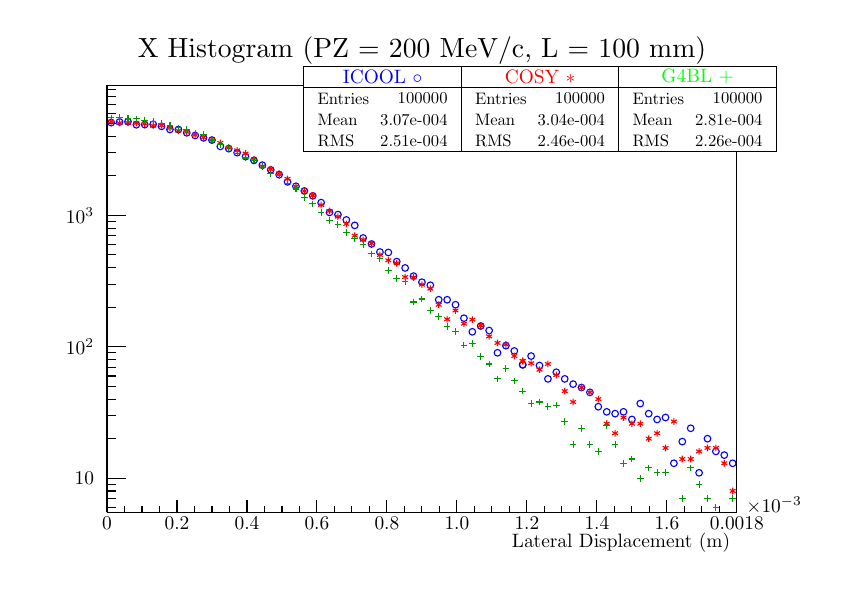
\begin{tikzpicture}
\definecolor{c}{rgb}{1,1,1};
\draw [color=c, fill=c] (0,0) rectangle (20,13.5632);
\draw [color=c, fill=c] (2,1.35632) rectangle (18,12.2069);
\definecolor{c}{rgb}{0,0,0};
\draw [c] (2,1.35632) -- (2,12.2069) -- (18,12.2069) -- (18,1.35632) -- (2,1.35632);
\definecolor{c}{rgb}{1,1,1};
\draw [color=c, fill=c] (2,1.35632) rectangle (18,12.2069);
\definecolor{c}{rgb}{0,0,0};
\draw [c] (2,1.35632) -- (2,12.2069) -- (18,12.2069) -- (18,1.35632) -- (2,1.35632);
\definecolor{c}{rgb}{0,0,1};
\foreach \P in
 {(2.10667,11.2557),(2.32,11.2727),(2.53333,11.2803),(2.74667,11.2016),(2.96,11.2051),(3.17333,11.214),(3.38667,11.1607),(3.6,11.082),(3.81333,11.0811),(4.02667,10.9972),(4.24,10.9291),(4.45333,10.8684),(4.66667,10.8125),(4.88,10.652),(5.09333,10.594
6),(5.30667,10.4924),(5.52,10.3923),(5.73333,10.2965),(5.94667,10.1748),(6.16,10.0557),(6.37333,9.93372),(6.58667,9.75064),(6.8,9.63834),(7.01333,9.51946),(7.22667,9.39614),(7.44,9.22356),(7.65333,8.97491),(7.86667,8.91876),(8.08,8.78386),(8.29333,8.
64552),(8.50667,8.32587),(8.72,8.17383),(8.93333,7.96855),(9.14667,7.95749),(9.36,7.7261),(9.57333,7.56426),(9.78667,7.35706),(10,7.20196),(10.2133,7.12513),(10.4267,6.75652),(10.64,6.75652),(10.8533,6.63037),(11.0667,6.28763),(11.28,5.94197),(11.493
3,6.09026),(11.7067,5.97505),(11.92,5.40881),(12.1333,5.59028),(12.3467,5.45635),(12.56,5.10528)}{\draw[mark options={color=c,fill=c},mark size=2.402402pt,mark=o] plot coordinates {\P};}
\foreach \P in
 {(12.56,5.10528),(12.7733,5.32594),(12.9867,5.08528),(13.2,4.74657),(13.4133,4.91451),(13.6267,4.74657),(13.84,4.61346),(14.0533,4.5273),(14.2667,4.40384),(14.48,4.03946),(14.6933,3.90953),(14.9067,3.8635),(15.12,3.90953),(15.3333,3.71593),(15.5467,
4.12003),(15.76,3.8635),(15.9733,3.71593),(16.1867,3.76681),(16.4,2.60351),(16.6133,3.15372),(16.8267,3.49243),(17.04,2.3613),(17.2533,3.22809),(17.4667,2.90456),(17.68,2.81098),(17.8933,2.60351)}{\draw[mark options={color=c,fill=c},mark
 size=2.402402pt,mark=o] plot coordinates {\P};}
\definecolor{c}{rgb}{1,1,1};
\draw [color=c, fill=c] (7,10.5115) rectangle (11,12.6816);
\definecolor{c}{rgb}{0,0,0};
\draw [c] (7,10.5115) -- (11,10.5115);
\draw [c] (11,10.5115) -- (11,12.6816);
\draw [c] (11,12.6816) -- (7,12.6816);
\draw [c] (7,12.6816) -- (7,10.5115);
\draw[color=blue](9,12.4103) node[scale=0.7, rotate=0]{ICOOL $\circ$};
\draw [c] (7,12.1391) -- (11,12.1391);
\draw [anchor= west] (7.2,11.8678) node[scale=0.6, rotate=0]{Entries };
\draw [anchor= east] (10.8,11.8678) node[scale=0.6, rotate=0]{ 100000};
\draw [anchor= west] (7.2,11.3253) node[scale=0.6, rotate=0]{Mean  };
\draw [anchor= east] (10.8,11.3253) node[scale=0.6, rotate=0]{ 3.07e-004};
\draw [anchor= west] (7.2,10.7828) node[scale=0.6, rotate=0]{RMS   };
\draw [anchor= east] (10.8,10.7828) node[scale=0.6, rotate=0]{ 2.51e-004};
\draw [c] (2,1.35632) -- (18,1.35632);
\draw [anchor= east] (18,0.596782) node[scale=0.7, rotate=0]{Lateral Displacement (m)};
\draw [c] (2,1.68184) -- (2,1.35632);
\draw [c] (2.44444,1.51908) -- (2.44444,1.35632);
\draw [c] (2.88889,1.51908) -- (2.88889,1.35632);
\draw [c] (3.33333,1.51908) -- (3.33333,1.35632);
\draw [c] (3.77778,1.68184) -- (3.77778,1.35632);
\draw [c] (4.22222,1.51908) -- (4.22222,1.35632);
\draw [c] (4.66667,1.51908) -- (4.66667,1.35632);
\draw [c] (5.11111,1.51908) -- (5.11111,1.35632);
\draw [c] (5.55556,1.68184) -- (5.55556,1.35632);
\draw [c] (6,1.51908) -- (6,1.35632);
\draw [c] (6.44444,1.51908) -- (6.44444,1.35632);
\draw [c] (6.88889,1.51908) -- (6.88889,1.35632);
\draw [c] (7.33333,1.68184) -- (7.33333,1.35632);
\draw [c] (7.77778,1.51908) -- (7.77778,1.35632);
\draw [c] (8.22222,1.51908) -- (8.22222,1.35632);
\draw [c] (8.66667,1.51908) -- (8.66667,1.35632);
\draw [c] (9.11111,1.68184) -- (9.11111,1.35632);
\draw [c] (9.55556,1.51908) -- (9.55556,1.35632);
\draw [c] (10,1.51908) -- (10,1.35632);
\draw [c] (10.4444,1.51908) -- (10.4444,1.35632);
\draw [c] (10.8889,1.68184) -- (10.8889,1.35632);
\draw [c] (11.3333,1.51908) -- (11.3333,1.35632);
\draw [c] (11.7778,1.51908) -- (11.7778,1.35632);
\draw [c] (12.2222,1.51908) -- (12.2222,1.35632);
\draw [c] (12.6667,1.68184) -- (12.6667,1.35632);
\draw [c] (13.1111,1.51908) -- (13.1111,1.35632);
\draw [c] (13.5556,1.51908) -- (13.5556,1.35632);
\draw [c] (14,1.51908) -- (14,1.35632);
\draw [c] (14.4444,1.68184) -- (14.4444,1.35632);
\draw [c] (14.8889,1.51908) -- (14.8889,1.35632);
\draw [c] (15.3333,1.51908) -- (15.3333,1.35632);
\draw [c] (15.7778,1.51908) -- (15.7778,1.35632);
\draw [c] (16.2222,1.68184) -- (16.2222,1.35632);
\draw [c] (16.6667,1.51908) -- (16.6667,1.35632);
\draw [c] (17.1111,1.51908) -- (17.1111,1.35632);
\draw [c] (17.5556,1.51908) -- (17.5556,1.35632);
\draw [c] (18,1.68184) -- (18,1.35632);
\draw [anchor=base] (2,0.908736) node[scale=0.7, rotate=0]{0};
\draw [anchor=base] (3.77778,0.908736) node[scale=0.7, rotate=0]{0.2};
\draw [anchor=base] (5.55556,0.908736) node[scale=0.7, rotate=0]{0.4};
\draw [anchor=base] (7.33333,0.908736) node[scale=0.7, rotate=0]{0.6};
\draw [anchor=base] (9.11111,0.908736) node[scale=0.7, rotate=0]{0.8};
\draw [anchor=base] (10.8889,0.908736) node[scale=0.7, rotate=0]{1.0};
\draw [anchor=base] (12.6667,0.908736) node[scale=0.7, rotate=0]{1.2};
\draw [anchor=base] (14.4444,0.908736) node[scale=0.7, rotate=0]{1.4};
\draw [anchor=base] (16.2222,0.908736) node[scale=0.7, rotate=0]{1.6};
\draw [anchor=base] (18,0.908736) node[scale=0.7, rotate=0]{0.0018};
\draw [anchor=base west] (18.07,1.35632) node[scale=0.7, rotate=0]{$\times10^{-3}$};
\draw [c] (2,1.35632) -- (2,12.2069);
\draw [c] (2.24,1.48247) -- (2,1.48247);
\draw [c] (2.24,1.70597) -- (2,1.70597);
\draw [c] (2.24,1.89958) -- (2,1.89958);
\draw [c] (2.24,2.07035) -- (2,2.07035);
\draw [c] (2.48,2.22311) -- (2,2.22311);
\draw [anchor= east] (1.844,2.22311) node[scale=0.7, rotate=0]{10};
\draw [c] (2.24,3.22809) -- (2,3.22809);
\draw [c] (2.24,3.81596) -- (2,3.81596);
\draw [c] (2.24,4.23306) -- (2,4.23306);
\draw [c] (2.24,4.55659) -- (2,4.55659);
\draw [c] (2.24,4.82094) -- (2,4.82094);
\draw [c] (2.24,5.04444) -- (2,5.04444);
\draw [c] (2.24,5.23804) -- (2,5.23804);
\draw [c] (2.24,5.40881) -- (2,5.40881);
\draw [c] (2.48,5.56157) -- (2,5.56157);
\draw [anchor= east] (1.844,5.56157) node[scale=0.7, rotate=0]{$10^{2}$};
\draw [c] (2.24,6.56655) -- (2,6.56655);
\draw [c] (2.24,7.15442) -- (2,7.15442);
\draw [c] (2.24,7.57152) -- (2,7.57152);
\draw [c] (2.24,7.89505) -- (2,7.89505);
\draw [c] (2.24,8.1594) -- (2,8.1594);
\draw [c] (2.24,8.3829) -- (2,8.3829);
\draw [c] (2.24,8.5765) -- (2,8.5765);
\draw [c] (2.24,8.74727) -- (2,8.74727);
\draw [c] (2.48,8.90003) -- (2,8.90003);
\draw [anchor= east] (1.844,8.90003) node[scale=0.7, rotate=0]{$10^{3}$};
\draw [c] (2.24,9.90501) -- (2,9.90501);
\draw [c] (2.24,10.4929) -- (2,10.4929);
\draw [c] (2.24,10.91) -- (2,10.91);
\draw [c] (2.24,11.2335) -- (2,11.2335);
\draw [c] (2.24,11.4979) -- (2,11.4979);
\draw [c] (2.24,11.7214) -- (2,11.7214);
\draw [c] (2.24,11.915) -- (2,11.915);
\draw [c] (2.24,12.0857) -- (2,12.0857);
\definecolor{c}{rgb}{1,1,1};
\draw [color=c, fill=c] (7,10.5115) rectangle (11,12.6816);
\definecolor{c}{rgb}{0,0,0};
\draw [c] (7,10.5115) -- (11,10.5115);
\draw [c] (11,10.5115) -- (11,12.6816);
\draw [c] (11,12.6816) -- (7,12.6816);
\draw [c] (7,12.6816) -- (7,10.5115);
\draw[color=blue](9,12.4103) node[scale=0.7, rotate=0]{ICOOL $\circ$};
\draw [c] (7,12.1391) -- (11,12.1391);
\draw [anchor= west] (7.2,11.8678) node[scale=0.6, rotate=0]{Entries };
\draw [anchor= east] (10.8,11.8678) node[scale=0.6, rotate=0]{ 100000};
\draw [anchor= west] (7.2,11.3253) node[scale=0.6, rotate=0]{Mean  };
\draw [anchor= east] (10.8,11.3253) node[scale=0.6, rotate=0]{ 3.07e-004};
\draw [anchor= west] (7.2,10.7828) node[scale=0.6, rotate=0]{RMS   };
\draw [anchor= east] (10.8,10.7828) node[scale=0.6, rotate=0]{ 2.51e-004};
\draw (10,13.0816) node[scale=1, rotate=0]{X Histogram (PZ = 200 MeV/c, L = 100 mm)};
\definecolor{c}{rgb}{1,0,0};
\foreach \P in
 {(2.10667,11.2812),(2.32,11.2436),(2.53333,11.2497),(2.74667,11.2448),(2.96,11.2268),(3.17333,11.1764),(3.38667,11.1846),(3.6,11.1208),(3.81333,11.0498),(4.02667,11.0199),(4.24,10.9415),(4.45333,10.88),(4.66667,10.8145),(4.88,10.7402),(5.09333,10.61
65),(5.30667,10.5507),(5.52,10.4705),(5.73333,10.3218),(5.94667,10.1462),(6.16,10.0732),(6.37333,9.96397),(6.58667,9.82759),(6.8,9.62961),(7.01333,9.51851),(7.22667,9.40435),(7.44,9.16317),(7.65333,9.01162),(7.86667,8.8663),(8.08,8.68136),(8.29333,8.
3829),(8.50667,8.27768),(8.72,8.18811),(8.93333,7.89506),(9.14667,7.75832),(9.36,7.68311),(9.57333,7.33162),(9.78667,7.32304),(10,7.13985),(10.2133,7.03877),(10.4267,6.63037),(10.64,6.26103),(10.8533,6.48453),(11.0667,6.14945),(11.28,6.25205),(11.493
3,6.10029),(11.7067,5.82592),(11.92,5.65967),(12.1333,5.61844),(12.3467,5.32594),(12.56,5.20133)}{\draw[mark options={color=c,fill=c},mark size=2.402402pt,mark=asterisk] plot coordinates {\P};}
\foreach \P in
 {(12.56,5.20133),(12.7733,5.14447),(12.9867,4.98093),(13.2,5.12501),(13.4133,4.8449),(13.6267,4.4357),(13.84,4.1587),(14.0533,4.5273),(14.2667,4.40384),(14.48,4.23306),(14.6933,3.60848),(14.9067,3.36628),(15.12,3.76681),(15.3333,3.60848),(15.5467,3.
60848),(15.76,3.22809),(15.9733,3.36628),(16.1867,2.99246),(16.4,3.6632),(16.6133,2.71095),(16.8267,2.71095),(17.04,2.90456),(17.2533,2.99246),(17.4667,2.99246),(17.68,2.60351),(17.8933,1.89958)}{\draw[mark options={color=c,fill=c},mark
 size=2.402402pt,mark=asterisk] plot coordinates {\P};}
\definecolor{c}{rgb}{1,1,1};
\draw [color=c, fill=c] (11,10.5115) rectangle (15,12.6816);
\definecolor{c}{rgb}{0,0,0};
\draw [c] (11,10.5115) -- (15,10.5115);
\draw [c] (15,10.5115) -- (15,12.6816);
\draw [c] (15,12.6816) -- (11,12.6816);
\draw [c] (11,12.6816) -- (11,10.5115);
\draw [color=red](13,12.4103) node[scale=0.7, rotate=0]{COSY $*$};
\draw [c] (11,12.1391) -- (15,12.1391);
\draw [anchor= west] (11.2,11.8678) node[scale=0.6, rotate=0]{Entries };
\draw [anchor= east] (14.8,11.8678) node[scale=0.6, rotate=0]{ 100000};
\draw [anchor= west] (11.2,11.3253) node[scale=0.6, rotate=0]{Mean  };
\draw [anchor= east] (14.8,11.3253) node[scale=0.6, rotate=0]{ 3.04e-004};
\draw [anchor= west] (11.2,10.7828) node[scale=0.6, rotate=0]{RMS   };
\draw [anchor= east] (14.8,10.7828) node[scale=0.6, rotate=0]{ 2.46e-004};
\definecolor{c}{rgb}{1,1,1};
\draw [color=c, fill=c] (11,10.5115) rectangle (15,12.6816);
\definecolor{c}{rgb}{0,0,0};
\draw [c] (11,10.5115) -- (15,10.5115);
\draw [c] (15,10.5115) -- (15,12.6816);
\draw [c] (15,12.6816) -- (11,12.6816);
\draw [c] (11,12.6816) -- (11,10.5115);
\draw [color=red](13,12.4103) node[scale=0.7, rotate=0]{COSY $*$};
\draw [c] (11,12.1391) -- (15,12.1391);
\draw [anchor= west] (11.2,11.8678) node[scale=0.6, rotate=0]{Entries };
\draw [anchor= east] (14.8,11.8678) node[scale=0.6, rotate=0]{ 100000};
\draw [anchor= west] (11.2,11.3253) node[scale=0.6, rotate=0]{Mean  };
\draw [anchor= east] (14.8,11.3253) node[scale=0.6, rotate=0]{ 3.04e-004};
\draw [anchor= west] (11.2,10.7828) node[scale=0.6, rotate=0]{RMS   };
\draw [anchor= east] (14.8,10.7828) node[scale=0.6, rotate=0]{ 2.46e-004};
\definecolor{c}{rgb}{0,0.6,0};
\foreach \P in
 {(2.10667,11.3754),(2.32,11.3947),(2.53333,11.363),(2.74667,11.3502),(2.96,11.3172),(3.17333,11.2823),(3.38667,11.2318),(3.6,11.1897),(3.81333,11.1217),(4.02667,11.073),(4.24,10.989),(4.45333,10.9528),(4.66667,10.8129),(4.88,10.701),(5.09333,10.6187
),(5.30667,10.4803),(5.52,10.3572),(5.73333,10.302),(5.94667,10.1252),(6.16,9.95349),(6.37333,9.90356),(6.58667,9.71802),(6.8,9.56965),(7.01333,9.35117),(7.22667,9.19072),(7.44,8.97491),(7.65333,8.76807),(7.86667,8.66781),(8.08,8.46543),(8.29333,8.30
416),(8.50667,8.15698),(8.72,7.92092),(8.93333,7.8115),(9.14667,7.49716),(9.36,7.28821),(9.57333,7.21129),(9.78667,6.69813),(10,6.77548),(10.2133,6.47684),(10.4267,6.33092),(10.64,6.08016),(10.8533,5.94197),(11.0667,5.60443),(11.28,5.64605),(11.4933,
5.30878),(11.7067,5.12501),(11.92,4.74657),(12.1333,5.00241),(12.3467,4.69478),(12.56,4.4357)}{\draw[mark options={color=c,fill=c},mark size=2.402402pt,mark=+] plot coordinates {\P};}
\foreach \P in
 {(12.56,4.4357),(12.7733,4.12003),(12.9867,4.1587),(13.2,4.03946),(13.4133,4.08031),(13.6267,3.6632),(13.84,3.07533),(14.0533,3.49243),(14.2667,3.07533),(14.48,2.90456),(14.6933,3.55162),(14.9067,3.07533),(15.12,2.60351),(15.3333,2.71095),(15.5467,2
.22311),(15.76,2.48745),(15.9733,2.3613),(16.1867,2.3613),(16.6133,1.70598),(16.8267,2.48745),(17.04,2.07035),(17.2533,1.70598),(17.4667,1.48248),(17.8933,1.70598)}{\draw[mark options={color=c,fill=c},mark size=2.402402pt,mark=+] plot coordinates
 {\P};}
\definecolor{c}{rgb}{1,1,1};
\draw [color=c, fill=c] (15,10.5115) rectangle (19,12.6816);
\definecolor{c}{rgb}{0,0,0};
\draw [c] (15,10.5115) -- (19,10.5115);
\draw [c] (19,10.5115) -- (19,12.6816);
\draw [c] (19,12.6816) -- (15,12.6816);
\draw [c] (15,12.6816) -- (15,10.5115);
\draw [color=green](17,12.4103) node[scale=0.7, rotate=0]{G4BL $+$};
\draw [c] (15,12.1391) -- (19,12.1391);
\draw [anchor= west] (15.2,11.8678) node[scale=0.6, rotate=0]{Entries };
\draw [anchor= east] (18.8,11.8678) node[scale=0.6, rotate=0]{ 100000};
\draw [anchor= west] (15.2,11.3253) node[scale=0.6, rotate=0]{Mean  };
\draw [anchor= east] (18.8,11.3253) node[scale=0.6, rotate=0]{ 2.81e-004};
\draw [anchor= west] (15.2,10.7828) node[scale=0.6, rotate=0]{RMS   };
\draw [anchor= east] (18.8,10.7828) node[scale=0.6, rotate=0]{ 2.26e-004};
\definecolor{c}{rgb}{1,1,1};
\draw [color=c, fill=c] (15,10.5115) rectangle (19,12.6816);
\definecolor{c}{rgb}{0,0,0};
\draw [c] (15,10.5115) -- (19,10.5115);
\draw [c] (19,10.5115) -- (19,12.6816);
\draw [c] (19,12.6816) -- (15,12.6816);
\draw [c] (15,12.6816) -- (15,10.5115);
\draw [color=green](17,12.4103) node[scale=0.7, rotate=0]{G4BL $+$};
\draw [c] (15,12.1391) -- (19,12.1391);
\draw [anchor= west] (15.2,11.8678) node[scale=0.6, rotate=0]{Entries };
\draw [anchor= east] (18.8,11.8678) node[scale=0.6, rotate=0]{ 100000};
\draw [anchor= west] (15.2,11.3253) node[scale=0.6, rotate=0]{Mean  };
\draw [anchor= east] (18.8,11.3253) node[scale=0.6, rotate=0]{ 2.81e-004};
\draw [anchor= west] (15.2,10.7828) node[scale=0.6, rotate=0]{RMS   };
\draw [anchor= east] (18.8,10.7828) node[scale=0.6, rotate=0]{ 2.26e-004};
\end{tikzpicture}
}\\
\frame{    \pgfdeclareplotmark{cross} {
\pgfpathmoveto{\pgfpoint{-0.3\pgfplotmarksize}{\pgfplotmarksize}}
\pgfpathlineto{\pgfpoint{+0.3\pgfplotmarksize}{\pgfplotmarksize}}
\pgfpathlineto{\pgfpoint{+0.3\pgfplotmarksize}{0.3\pgfplotmarksize}}
\pgfpathlineto{\pgfpoint{+1\pgfplotmarksize}{0.3\pgfplotmarksize}}
\pgfpathlineto{\pgfpoint{+1\pgfplotmarksize}{-0.3\pgfplotmarksize}}
\pgfpathlineto{\pgfpoint{+0.3\pgfplotmarksize}{-0.3\pgfplotmarksize}}
\pgfpathlineto{\pgfpoint{+0.3\pgfplotmarksize}{-1.\pgfplotmarksize}}
\pgfpathlineto{\pgfpoint{-0.3\pgfplotmarksize}{-1.\pgfplotmarksize}}
\pgfpathlineto{\pgfpoint{-0.3\pgfplotmarksize}{-0.3\pgfplotmarksize}}
\pgfpathlineto{\pgfpoint{-1.\pgfplotmarksize}{-0.3\pgfplotmarksize}}
\pgfpathlineto{\pgfpoint{-1.\pgfplotmarksize}{0.3\pgfplotmarksize}}
\pgfpathlineto{\pgfpoint{-0.3\pgfplotmarksize}{0.3\pgfplotmarksize}}
\pgfpathclose
\pgfusepathqstroke
}
\pgfdeclareplotmark{cross*} {
\pgfpathmoveto{\pgfpoint{-0.3\pgfplotmarksize}{\pgfplotmarksize}}
\pgfpathlineto{\pgfpoint{+0.3\pgfplotmarksize}{\pgfplotmarksize}}
\pgfpathlineto{\pgfpoint{+0.3\pgfplotmarksize}{0.3\pgfplotmarksize}}
\pgfpathlineto{\pgfpoint{+1\pgfplotmarksize}{0.3\pgfplotmarksize}}
\pgfpathlineto{\pgfpoint{+1\pgfplotmarksize}{-0.3\pgfplotmarksize}}
\pgfpathlineto{\pgfpoint{+0.3\pgfplotmarksize}{-0.3\pgfplotmarksize}}
\pgfpathlineto{\pgfpoint{+0.3\pgfplotmarksize}{-1.\pgfplotmarksize}}
\pgfpathlineto{\pgfpoint{-0.3\pgfplotmarksize}{-1.\pgfplotmarksize}}
\pgfpathlineto{\pgfpoint{-0.3\pgfplotmarksize}{-0.3\pgfplotmarksize}}
\pgfpathlineto{\pgfpoint{-1.\pgfplotmarksize}{-0.3\pgfplotmarksize}}
\pgfpathlineto{\pgfpoint{-1.\pgfplotmarksize}{0.3\pgfplotmarksize}}
\pgfpathlineto{\pgfpoint{-0.3\pgfplotmarksize}{0.3\pgfplotmarksize}}
\pgfpathclose
\pgfusepathqfillstroke
}
\pgfdeclareplotmark{newstar} {
\pgfpathmoveto{\pgfqpoint{0pt}{\pgfplotmarksize}}
\pgfpathlineto{\pgfqpointpolar{44}{0.5\pgfplotmarksize}}
\pgfpathlineto{\pgfqpointpolar{18}{\pgfplotmarksize}}
\pgfpathlineto{\pgfqpointpolar{-20}{0.5\pgfplotmarksize}}
\pgfpathlineto{\pgfqpointpolar{-54}{\pgfplotmarksize}}
\pgfpathlineto{\pgfqpointpolar{-90}{0.5\pgfplotmarksize}}
\pgfpathlineto{\pgfqpointpolar{234}{\pgfplotmarksize}}
\pgfpathlineto{\pgfqpointpolar{198}{0.5\pgfplotmarksize}}
\pgfpathlineto{\pgfqpointpolar{162}{\pgfplotmarksize}}
\pgfpathlineto{\pgfqpointpolar{134}{0.5\pgfplotmarksize}}
\pgfpathclose
\pgfusepathqstroke
}
\pgfdeclareplotmark{newstar*} {
\pgfpathmoveto{\pgfqpoint{0pt}{\pgfplotmarksize}}
\pgfpathlineto{\pgfqpointpolar{44}{0.5\pgfplotmarksize}}
\pgfpathlineto{\pgfqpointpolar{18}{\pgfplotmarksize}}
\pgfpathlineto{\pgfqpointpolar{-20}{0.5\pgfplotmarksize}}
\pgfpathlineto{\pgfqpointpolar{-54}{\pgfplotmarksize}}
\pgfpathlineto{\pgfqpointpolar{-90}{0.5\pgfplotmarksize}}
\pgfpathlineto{\pgfqpointpolar{234}{\pgfplotmarksize}}
\pgfpathlineto{\pgfqpointpolar{198}{0.5\pgfplotmarksize}}
\pgfpathlineto{\pgfqpointpolar{162}{\pgfplotmarksize}}
\pgfpathlineto{\pgfqpointpolar{134}{0.5\pgfplotmarksize}}
\pgfpathclose
\pgfusepathqfillstroke
}
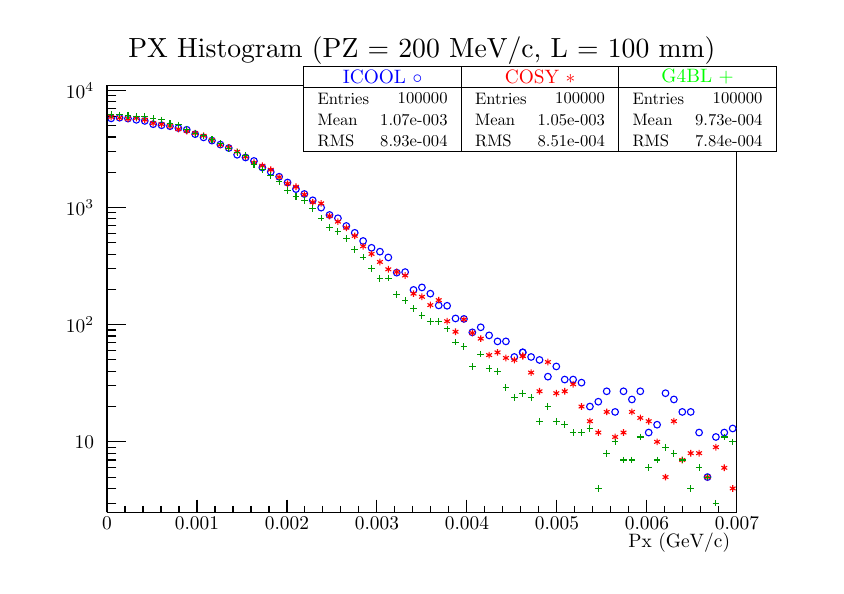
\begin{tikzpicture}
\definecolor{c}{rgb}{1,1,1};
\draw [color=c, fill=c] (0,0) rectangle (20,13.5632);
\draw [color=c, fill=c] (2,1.35632) rectangle (18,12.2069);
\definecolor{c}{rgb}{0,0,0};
\draw [c] (2,1.35632) -- (2,12.2069) -- (18,12.2069) -- (18,1.35632) -- (2,1.35632);
\definecolor{c}{rgb}{1,1,1};
\draw [color=c, fill=c] (2,1.35632) rectangle (18,12.2069);
\definecolor{c}{rgb}{0,0,0};
\draw [c] (2,1.35632) -- (2,12.2069) -- (18,12.2069) -- (18,1.35632) -- (2,1.35632);
\definecolor{c}{rgb}{0,0,1};
\foreach \P in
 {(2.10667,11.363),(2.32,11.381),(2.53333,11.3589),(2.74667,11.3264),(2.96,11.2986),(3.17333,11.2154),(3.38667,11.189),(3.6,11.1644),(3.81333,11.1176),(4.02667,11.074),(4.24,10.9626),(4.45333,10.8802),(4.66667,10.7993),(4.88,10.6983),(5.09333,10.6099
),(5.30667,10.4389),(5.52,10.3697),(5.73333,10.2817),(5.94667,10.1163),(6.16,10.0032),(6.37333,9.88149),(6.58667,9.73447),(6.8,9.56765),(7.01333,9.44313),(7.22667,9.2831),(7.44,9.09653),(7.65333,8.9102),(7.86667,8.8268),(8.08,8.63078),(8.29333,8.4560
9),(8.50667,8.24906),(8.72,8.07579),(8.93333,7.97804),(9.14667,7.83159),(9.36,7.44479),(9.57333,7.45866),(9.78667,7.00624),(10,7.06992),(10.2133,6.91148),(10.4267,6.61253),(10.64,6.60365),(10.8533,6.28142),(11.0667,6.26993),(11.28,5.92857),(11.4933,6
.05719),(11.7067,5.85116),(11.92,5.69895),(12.1333,5.69895),(12.3467,5.30302),(12.56,5.41952)}{\draw[mark options={color=c,fill=c},mark size=2.402402pt,mark=o] plot coordinates {\P};}
\foreach \P in
 {(12.56,5.41952),(12.7733,5.30302),(12.9867,5.22772),(13.2,4.80319),(13.4133,5.06252),(13.6267,4.72933),(13.84,4.72933),(14.0533,4.65098),(14.2667,4.04359),(14.48,4.16676),(14.6933,4.43142),(14.9067,3.90743),(15.12,4.43142),(15.3333,4.22421),(15.546
7,4.43142),(15.76,3.38345),(15.9733,3.58266),(16.1867,4.38265),(16.4,4.22421),(16.6133,3.90743),(16.8267,3.90743),(17.04,3.38345),(17.2533,2.25208),(17.4667,3.27101),(17.68,3.38345),(17.8933,3.48689)}{\draw[mark options={color=c,fill=c},mark
 size=2.402402pt,mark=o] plot coordinates {\P};}
\definecolor{c}{rgb}{1,1,1};
\draw [color=c, fill=c] (7,10.5115) rectangle (11,12.6816);
\definecolor{c}{rgb}{0,0,0};
\draw [c] (7,10.5115) -- (11,10.5115);
\draw [c] (11,10.5115) -- (11,12.6816);
\draw [c] (11,12.6816) -- (7,12.6816);
\draw [c] (7,12.6816) -- (7,10.5115);
\draw[color=blue](9,12.4103) node[scale=0.7, rotate=0]{ICOOL $\circ$};
\draw [c] (7,12.1391) -- (11,12.1391);
\draw [anchor= west] (7.2,11.8678) node[scale=0.6, rotate=0]{Entries };
\draw [anchor= east] (10.8,11.8678) node[scale=0.6, rotate=0]{ 100000};
\draw [anchor= west] (7.2,11.3253) node[scale=0.6, rotate=0]{Mean  };
\draw [anchor= east] (10.8,11.3253) node[scale=0.6, rotate=0]{ 1.07e-003};
\draw [anchor= west] (7.2,10.7828) node[scale=0.6, rotate=0]{RMS   };
\draw [anchor= east] (10.8,10.7828) node[scale=0.6, rotate=0]{ 8.93e-004};
\draw [c] (2,1.35632) -- (18,1.35632);
\draw [anchor= east] (18,0.596782) node[scale=0.7, rotate=0]{Px (GeV/c)};
\draw [c] (2,1.68184) -- (2,1.35632);
\draw [c] (2.45714,1.51908) -- (2.45714,1.35632);
\draw [c] (2.91429,1.51908) -- (2.91429,1.35632);
\draw [c] (3.37143,1.51908) -- (3.37143,1.35632);
\draw [c] (3.82857,1.51908) -- (3.82857,1.35632);
\draw [c] (4.28571,1.68184) -- (4.28571,1.35632);
\draw [c] (4.74286,1.51908) -- (4.74286,1.35632);
\draw [c] (5.2,1.51908) -- (5.2,1.35632);
\draw [c] (5.65714,1.51908) -- (5.65714,1.35632);
\draw [c] (6.11429,1.51908) -- (6.11429,1.35632);
\draw [c] (6.57143,1.68184) -- (6.57143,1.35632);
\draw [c] (7.02857,1.51908) -- (7.02857,1.35632);
\draw [c] (7.48571,1.51908) -- (7.48571,1.35632);
\draw [c] (7.94286,1.51908) -- (7.94286,1.35632);
\draw [c] (8.4,1.51908) -- (8.4,1.35632);
\draw [c] (8.85714,1.68184) -- (8.85714,1.35632);
\draw [c] (9.31429,1.51908) -- (9.31429,1.35632);
\draw [c] (9.77143,1.51908) -- (9.77143,1.35632);
\draw [c] (10.2286,1.51908) -- (10.2286,1.35632);
\draw [c] (10.6857,1.51908) -- (10.6857,1.35632);
\draw [c] (11.1429,1.68184) -- (11.1429,1.35632);
\draw [c] (11.6,1.51908) -- (11.6,1.35632);
\draw [c] (12.0571,1.51908) -- (12.0571,1.35632);
\draw [c] (12.5143,1.51908) -- (12.5143,1.35632);
\draw [c] (12.9714,1.51908) -- (12.9714,1.35632);
\draw [c] (13.4286,1.68184) -- (13.4286,1.35632);
\draw [c] (13.8857,1.51908) -- (13.8857,1.35632);
\draw [c] (14.3429,1.51908) -- (14.3429,1.35632);
\draw [c] (14.8,1.51908) -- (14.8,1.35632);
\draw [c] (15.2571,1.51908) -- (15.2571,1.35632);
\draw [c] (15.7143,1.68184) -- (15.7143,1.35632);
\draw [c] (16.1714,1.51908) -- (16.1714,1.35632);
\draw [c] (16.6286,1.51908) -- (16.6286,1.35632);
\draw [c] (17.0857,1.51908) -- (17.0857,1.35632);
\draw [c] (17.5429,1.51908) -- (17.5429,1.35632);
\draw [c] (18,1.68184) -- (18,1.35632);
\draw [c] (18,1.68184) -- (18,1.35632);
\draw [anchor=base] (2,0.908736) node[scale=0.7, rotate=0]{0};
\draw [anchor=base] (4.28571,0.908736) node[scale=0.7, rotate=0]{0.001};
\draw [anchor=base] (6.57143,0.908736) node[scale=0.7, rotate=0]{0.002};
\draw [anchor=base] (8.85714,0.908736) node[scale=0.7, rotate=0]{0.003};
\draw [anchor=base] (11.1429,0.908736) node[scale=0.7, rotate=0]{0.004};
\draw [anchor=base] (13.4286,0.908736) node[scale=0.7, rotate=0]{0.005};
\draw [anchor=base] (15.7143,0.908736) node[scale=0.7, rotate=0]{0.006};
\draw [anchor=base] (18,0.908736) node[scale=0.7, rotate=0]{0.007};
\draw [c] (2,1.35632) -- (2,12.2069);
\draw [c] (2.24,1.59193) -- (2,1.59193);
\draw [c] (2.24,1.96371) -- (2,1.96371);
\draw [c] (2.24,2.25208) -- (2,2.25208);
\draw [c] (2.24,2.48769) -- (2,2.48769);
\draw [c] (2.24,2.6869) -- (2,2.6869);
\draw [c] (2.24,2.85946) -- (2,2.85946);
\draw [c] (2.24,3.01168) -- (2,3.01168);
\draw [c] (2.48,3.14783) -- (2,3.14783);
\draw [anchor= east] (1.844,3.14783) node[scale=0.7, rotate=0]{10};
\draw [c] (2.24,4.04359) -- (2,4.04359);
\draw [c] (2.24,4.56757) -- (2,4.56757);
\draw [c] (2.24,4.93935) -- (2,4.93935);
\draw [c] (2.24,5.22772) -- (2,5.22772);
\draw [c] (2.24,5.46333) -- (2,5.46333);
\draw [c] (2.24,5.66254) -- (2,5.66254);
\draw [c] (2.24,5.8351) -- (2,5.8351);
\draw [c] (2.24,5.98732) -- (2,5.98732);
\draw [c] (2.48,6.12347) -- (2,6.12347);
\draw [anchor= east] (1.844,6.12347) node[scale=0.7, rotate=0]{$10^{2}$};
\draw [c] (2.24,7.01923) -- (2,7.01923);
\draw [c] (2.24,7.54322) -- (2,7.54322);
\draw [c] (2.24,7.91499) -- (2,7.91499);
\draw [c] (2.24,8.20336) -- (2,8.20336);
\draw [c] (2.24,8.43897) -- (2,8.43897);
\draw [c] (2.24,8.63818) -- (2,8.63818);
\draw [c] (2.24,8.81075) -- (2,8.81075);
\draw [c] (2.24,8.96296) -- (2,8.96296);
\draw [c] (2.48,9.09911) -- (2,9.09911);
\draw [anchor= east] (1.844,9.09911) node[scale=0.7, rotate=0]{$10^{3}$};
\draw [c] (2.24,9.99487) -- (2,9.99487);
\draw [c] (2.24,10.5189) -- (2,10.5189);
\draw [c] (2.24,10.8906) -- (2,10.8906);
\draw [c] (2.24,11.179) -- (2,11.179);
\draw [c] (2.24,11.4146) -- (2,11.4146);
\draw [c] (2.24,11.6138) -- (2,11.6138);
\draw [c] (2.24,11.7864) -- (2,11.7864);
\draw [c] (2.24,11.9386) -- (2,11.9386);
\draw [c] (2.48,12.0748) -- (2,12.0748);
\draw [anchor= east] (1.844,12.0748) node[scale=0.7, rotate=0]{$10^{4}$};
\definecolor{c}{rgb}{1,1,1};
\draw [color=c, fill=c] (7,10.5115) rectangle (11,12.6816);
\definecolor{c}{rgb}{0,0,0};
\draw [c] (7,10.5115) -- (11,10.5115);
\draw [c] (11,10.5115) -- (11,12.6816);
\draw [c] (11,12.6816) -- (7,12.6816);
\draw [c] (7,12.6816) -- (7,10.5115);
\draw[color=blue](9,12.4103) node[scale=0.7, rotate=0]{ICOOL $\circ$};
\draw [c] (7,12.1391) -- (11,12.1391);
\draw [anchor= west] (7.2,11.8678) node[scale=0.6, rotate=0]{Entries };
\draw [anchor= east] (10.8,11.8678) node[scale=0.6, rotate=0]{ 100000};
\draw [anchor= west] (7.2,11.3253) node[scale=0.6, rotate=0]{Mean  };
\draw [anchor= east] (10.8,11.3253) node[scale=0.6, rotate=0]{ 1.07e-003};
\draw [anchor= west] (7.2,10.7828) node[scale=0.6, rotate=0]{RMS   };
\draw [anchor= east] (10.8,10.7828) node[scale=0.6, rotate=0]{ 8.93e-004};
\draw (10,13.0816) node[scale=1, rotate=0]{PX Histogram (PZ = 200 MeV/c, L = 100 mm)};
\definecolor{c}{rgb}{1,0,0};
\foreach \P in
 {(2.10667,11.3984),(2.32,11.3777),(2.53333,11.3533),(2.74667,11.3708),(2.96,11.3296),(3.17333,11.2411),(3.38667,11.2137),(3.6,11.171),(3.81333,11.0905),(4.02667,11.0423),(4.24,10.9889),(4.45333,10.921),(4.66667,10.8138),(4.88,10.6916),(5.09333,10.62
19),(5.30667,10.5184),(5.52,10.3913),(5.73333,10.2353),(5.94667,10.1614),(6.16,10.0598),(6.37333,9.87157),(6.58667,9.7057),(6.8,9.62568),(7.01333,9.42719),(7.22667,9.23514),(7.44,9.20454),(7.65333,8.88147),(7.86667,8.74105),(8.08,8.5835),(8.29333,8.3
7947),(8.50667,8.11512),(8.72,7.92143),(8.93333,7.71632),(9.14667,7.53023),(9.36,7.46325),(9.57333,7.37311),(9.78667,6.91148),(10,6.83181),(10.2133,6.62135),(10.4267,6.74692),(10.64,6.21091),(10.8533,5.94351),(11.0667,6.25834),(11.28,5.91345),(11.493
3,5.76882),(11.7067,5.35089),(11.92,5.41952),(12.1333,5.2784),(12.3467,5.22772),(12.56,5.32718)}{\draw[mark options={color=c,fill=c},mark size=2.402402pt,mark=asterisk] plot coordinates {\P};}
\foreach \P in
 {(12.56,5.32718),(12.7733,4.90663),(12.9867,4.43142),(13.2,5.17496),(13.4133,4.38265),(13.6267,4.43142),(13.84,4.60995),(14.0533,4.04359),(14.2667,3.67182),(14.48,3.38345),(14.6933,3.90743),(14.9067,3.27101),(15.12,3.38345),(15.3333,3.90743),(15.546
7,3.75522),(15.76,3.67182),(15.9733,3.14784),(16.1867,2.25208),(16.4,3.67182),(16.6133,2.6869),(16.8267,2.85947),(17.04,2.85947),(17.2533,2.25208),(17.4667,3.01168),(17.68,2.48769),(17.8933,1.96371)}{\draw[mark options={color=c,fill=c},mark
 size=2.402402pt,mark=asterisk] plot coordinates {\P};}
\definecolor{c}{rgb}{1,1,1};
\draw [color=c, fill=c] (11,10.5115) rectangle (15,12.6816);
\definecolor{c}{rgb}{0,0,0};
\draw [c] (11,10.5115) -- (15,10.5115);
\draw [c] (15,10.5115) -- (15,12.6816);
\draw [c] (15,12.6816) -- (11,12.6816);
\draw [c] (11,12.6816) -- (11,10.5115);
\draw [color=red](13,12.4103) node[scale=0.7, rotate=0]{COSY $*$};
\draw [c] (11,12.1391) -- (15,12.1391);
\draw [anchor= west] (11.2,11.8678) node[scale=0.6, rotate=0]{Entries };
\draw [anchor= east] (14.8,11.8678) node[scale=0.6, rotate=0]{ 100000};
\draw [anchor= west] (11.2,11.3253) node[scale=0.6, rotate=0]{Mean  };
\draw [anchor= east] (14.8,11.3253) node[scale=0.6, rotate=0]{ 1.05e-003};
\draw [anchor= west] (11.2,10.7828) node[scale=0.6, rotate=0]{RMS   };
\draw [anchor= east] (14.8,10.7828) node[scale=0.6, rotate=0]{ 8.51e-004};
\definecolor{c}{rgb}{1,1,1};
\draw [color=c, fill=c] (11,10.5115) rectangle (15,12.6816);
\definecolor{c}{rgb}{0,0,0};
\draw [c] (11,10.5115) -- (15,10.5115);
\draw [c] (15,10.5115) -- (15,12.6816);
\draw [c] (15,12.6816) -- (11,12.6816);
\draw [c] (11,12.6816) -- (11,10.5115);
\draw [color=red](13,12.4103) node[scale=0.7, rotate=0]{COSY $*$};
\draw [c] (11,12.1391) -- (15,12.1391);
\draw [anchor= west] (11.2,11.8678) node[scale=0.6, rotate=0]{Entries };
\draw [anchor= east] (14.8,11.8678) node[scale=0.6, rotate=0]{ 100000};
\draw [anchor= west] (11.2,11.3253) node[scale=0.6, rotate=0]{Mean  };
\draw [anchor= east] (14.8,11.3253) node[scale=0.6, rotate=0]{ 1.05e-003};
\draw [anchor= west] (11.2,10.7828) node[scale=0.6, rotate=0]{RMS   };
\draw [anchor= east] (14.8,10.7828) node[scale=0.6, rotate=0]{ 8.51e-004};
\definecolor{c}{rgb}{0,0.6,0};
\foreach \P in
 {(2.10667,11.4597),(2.32,11.4528),(2.53333,11.4326),(2.74667,11.4066),(2.96,11.4058),(3.17333,11.3587),(3.38667,11.3248),(3.6,11.2299),(3.81333,11.197),(4.02667,11.083),(4.24,10.9763),(4.45333,10.9181),(4.66667,10.8348),(4.88,10.7195),(5.09333,10.60
23),(5.30667,10.4919),(5.52,10.4162),(5.73333,10.1994),(5.94667,10.0665),(6.16,9.91971),(6.37333,9.75018),(6.58667,9.53209),(6.8,9.37502),(7.01333,9.28085),(7.22667,9.07037),(7.44,8.82999),(7.65333,8.59501),(7.86667,8.49173),(8.08,8.31946),(8.29333,8
.03227),(8.50667,7.83846),(8.72,7.5518),(8.93333,7.30242),(9.14667,7.3076),(9.36,6.89735),(9.57333,6.73891),(9.78667,6.53031),(10,6.34828),(10.2133,6.21091),(10.4267,6.21091),(10.64,6.01572),(10.8533,5.68087),(11.0667,5.56677),(11.28,5.06252),(11.493
3,5.37417),(11.7067,5.0024),(11.92,4.93935),(12.1333,4.52377),(12.3467,4.27921),(12.56,4.38265)}{\draw[mark options={color=c,fill=c},mark size=2.402402pt,mark=+] plot coordinates {\P};}
\foreach \P in
 {(12.56,4.38265),(12.7733,4.27921),(12.9867,3.67182),(13.2,4.04359),(13.4133,3.67182),(13.6267,3.58266),(13.84,3.38345),(14.0533,3.38345),(14.2667,3.48689),(14.48,1.96371),(14.6933,2.85947),(14.9067,3.14784),(15.12,2.6869),(15.3333,2.6869),(15.5467,
3.27101),(15.76,2.48769),(15.9733,2.6869),(16.1867,3.01168),(16.4,2.85947),(16.6133,2.6869),(16.8267,1.96371),(17.04,2.48769),(17.2533,2.25208),(17.4667,1.59194),(17.68,3.27101),(17.8933,3.14784)}{\draw[mark options={color=c,fill=c},mark
 size=2.402402pt,mark=+] plot coordinates {\P};}
\definecolor{c}{rgb}{1,1,1};
\draw [color=c, fill=c] (15,10.5115) rectangle (19,12.6816);
\definecolor{c}{rgb}{0,0,0};
\draw [c] (15,10.5115) -- (19,10.5115);
\draw [c] (19,10.5115) -- (19,12.6816);
\draw [c] (19,12.6816) -- (15,12.6816);
\draw [c] (15,12.6816) -- (15,10.5115);
\draw [color=green](17,12.4103) node[scale=0.7, rotate=0]{G4BL $+$};
\draw [c] (15,12.1391) -- (19,12.1391);
\draw [anchor= west] (15.2,11.8678) node[scale=0.6, rotate=0]{Entries };
\draw [anchor= east] (18.8,11.8678) node[scale=0.6, rotate=0]{ 100000};
\draw [anchor= west] (15.2,11.3253) node[scale=0.6, rotate=0]{Mean  };
\draw [anchor= east] (18.8,11.3253) node[scale=0.6, rotate=0]{ 9.73e-004};
\draw [anchor= west] (15.2,10.7828) node[scale=0.6, rotate=0]{RMS   };
\draw [anchor= east] (18.8,10.7828) node[scale=0.6, rotate=0]{ 7.84e-004};
\definecolor{c}{rgb}{1,1,1};
\draw [color=c, fill=c] (15,10.5115) rectangle (19,12.6816);
\definecolor{c}{rgb}{0,0,0};
\draw [c] (15,10.5115) -- (19,10.5115);
\draw [c] (19,10.5115) -- (19,12.6816);
\draw [c] (19,12.6816) -- (15,12.6816);
\draw [c] (15,12.6816) -- (15,10.5115);
\draw [color=green](17,12.4103) node[scale=0.7, rotate=0]{G4BL $+$};
\draw [c] (15,12.1391) -- (19,12.1391);
\draw [anchor= west] (15.2,11.8678) node[scale=0.6, rotate=0]{Entries };
\draw [anchor= east] (18.8,11.8678) node[scale=0.6, rotate=0]{ 100000};
\draw [anchor= west] (15.2,11.3253) node[scale=0.6, rotate=0]{Mean  };
\draw [anchor= east] (18.8,11.3253) node[scale=0.6, rotate=0]{ 9.73e-004};
\draw [anchor= west] (15.2,10.7828) node[scale=0.6, rotate=0]{RMS   };
\draw [anchor= east] (18.8,10.7828) node[scale=0.6, rotate=0]{ 7.84e-004};
\end{tikzpicture}
}\\
\frame{\pgfdeclareplotmark{cross} {
\pgfpathmoveto{\pgfpoint{-0.3\pgfplotmarksize}{\pgfplotmarksize}}
\pgfpathlineto{\pgfpoint{+0.3\pgfplotmarksize}{\pgfplotmarksize}}
\pgfpathlineto{\pgfpoint{+0.3\pgfplotmarksize}{0.3\pgfplotmarksize}}
\pgfpathlineto{\pgfpoint{+1\pgfplotmarksize}{0.3\pgfplotmarksize}}
\pgfpathlineto{\pgfpoint{+1\pgfplotmarksize}{-0.3\pgfplotmarksize}}
\pgfpathlineto{\pgfpoint{+0.3\pgfplotmarksize}{-0.3\pgfplotmarksize}}
\pgfpathlineto{\pgfpoint{+0.3\pgfplotmarksize}{-1.\pgfplotmarksize}}
\pgfpathlineto{\pgfpoint{-0.3\pgfplotmarksize}{-1.\pgfplotmarksize}}
\pgfpathlineto{\pgfpoint{-0.3\pgfplotmarksize}{-0.3\pgfplotmarksize}}
\pgfpathlineto{\pgfpoint{-1.\pgfplotmarksize}{-0.3\pgfplotmarksize}}
\pgfpathlineto{\pgfpoint{-1.\pgfplotmarksize}{0.3\pgfplotmarksize}}
\pgfpathlineto{\pgfpoint{-0.3\pgfplotmarksize}{0.3\pgfplotmarksize}}
\pgfpathclose
\pgfusepathqstroke
}
\pgfdeclareplotmark{cross*} {
\pgfpathmoveto{\pgfpoint{-0.3\pgfplotmarksize}{\pgfplotmarksize}}
\pgfpathlineto{\pgfpoint{+0.3\pgfplotmarksize}{\pgfplotmarksize}}
\pgfpathlineto{\pgfpoint{+0.3\pgfplotmarksize}{0.3\pgfplotmarksize}}
\pgfpathlineto{\pgfpoint{+1\pgfplotmarksize}{0.3\pgfplotmarksize}}
\pgfpathlineto{\pgfpoint{+1\pgfplotmarksize}{-0.3\pgfplotmarksize}}
\pgfpathlineto{\pgfpoint{+0.3\pgfplotmarksize}{-0.3\pgfplotmarksize}}
\pgfpathlineto{\pgfpoint{+0.3\pgfplotmarksize}{-1.\pgfplotmarksize}}
\pgfpathlineto{\pgfpoint{-0.3\pgfplotmarksize}{-1.\pgfplotmarksize}}
\pgfpathlineto{\pgfpoint{-0.3\pgfplotmarksize}{-0.3\pgfplotmarksize}}
\pgfpathlineto{\pgfpoint{-1.\pgfplotmarksize}{-0.3\pgfplotmarksize}}
\pgfpathlineto{\pgfpoint{-1.\pgfplotmarksize}{0.3\pgfplotmarksize}}
\pgfpathlineto{\pgfpoint{-0.3\pgfplotmarksize}{0.3\pgfplotmarksize}}
\pgfpathclose
\pgfusepathqfillstroke
}
\pgfdeclareplotmark{newstar} {
\pgfpathmoveto{\pgfqpoint{0pt}{\pgfplotmarksize}}
\pgfpathlineto{\pgfqpointpolar{44}{0.5\pgfplotmarksize}}
\pgfpathlineto{\pgfqpointpolar{18}{\pgfplotmarksize}}
\pgfpathlineto{\pgfqpointpolar{-20}{0.5\pgfplotmarksize}}
\pgfpathlineto{\pgfqpointpolar{-54}{\pgfplotmarksize}}
\pgfpathlineto{\pgfqpointpolar{-90}{0.5\pgfplotmarksize}}
\pgfpathlineto{\pgfqpointpolar{234}{\pgfplotmarksize}}
\pgfpathlineto{\pgfqpointpolar{198}{0.5\pgfplotmarksize}}
\pgfpathlineto{\pgfqpointpolar{162}{\pgfplotmarksize}}
\pgfpathlineto{\pgfqpointpolar{134}{0.5\pgfplotmarksize}}
\pgfpathclose
\pgfusepathqstroke
}
\pgfdeclareplotmark{newstar*} {
\pgfpathmoveto{\pgfqpoint{0pt}{\pgfplotmarksize}}
\pgfpathlineto{\pgfqpointpolar{44}{0.5\pgfplotmarksize}}
\pgfpathlineto{\pgfqpointpolar{18}{\pgfplotmarksize}}
\pgfpathlineto{\pgfqpointpolar{-20}{0.5\pgfplotmarksize}}
\pgfpathlineto{\pgfqpointpolar{-54}{\pgfplotmarksize}}
\pgfpathlineto{\pgfqpointpolar{-90}{0.5\pgfplotmarksize}}
\pgfpathlineto{\pgfqpointpolar{234}{\pgfplotmarksize}}
\pgfpathlineto{\pgfqpointpolar{198}{0.5\pgfplotmarksize}}
\pgfpathlineto{\pgfqpointpolar{162}{\pgfplotmarksize}}
\pgfpathlineto{\pgfqpointpolar{134}{0.5\pgfplotmarksize}}
\pgfpathclose
\pgfusepathqfillstroke
}
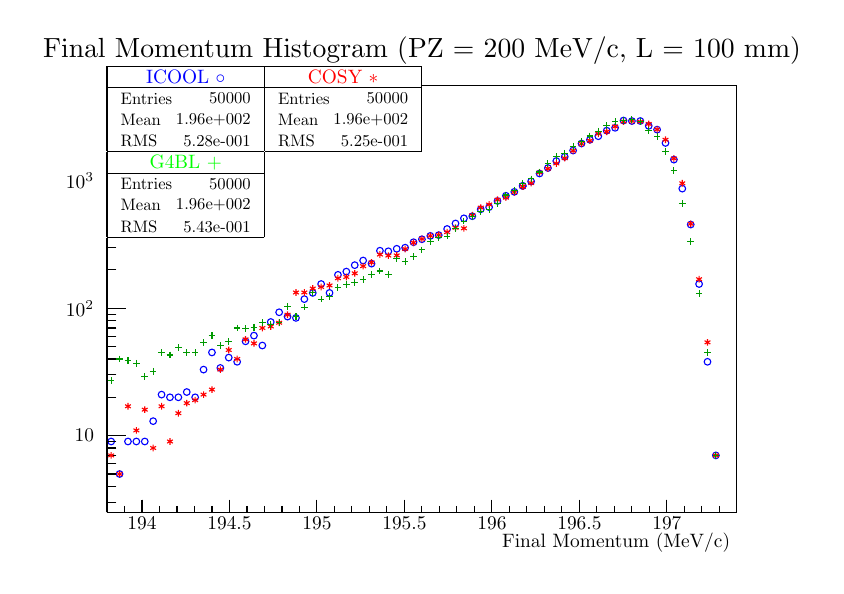
\begin{tikzpicture}
\definecolor{c}{rgb}{1,1,1};
\draw [color=c, fill=c] (0,0) rectangle (20,13.5632);
\draw [color=c, fill=c] (2,1.35632) rectangle (18,12.2069);
\definecolor{c}{rgb}{0,0,0};
\draw [c] (2,1.35632) -- (2,12.2069) -- (18,12.2069) -- (18,1.35632) -- (2,1.35632);
\definecolor{c}{rgb}{1,1,1};
\draw [color=c, fill=c] (2,1.35632) rectangle (18,12.2069);
\definecolor{c}{rgb}{0,0,0};
\draw [c] (2,1.35632) -- (2,12.2069) -- (18,12.2069) -- (18,1.35632) -- (2,1.35632);
\definecolor{c}{rgb}{0,0,1};
\foreach \P in
 {(2.10667,3.15643),(2.32,2.33041),(2.53333,3.15643),(2.74667,3.15643),(2.96,3.15643),(3.17333,3.6732),(3.38667,4.34715),(3.6,4.27858),(3.81333,4.27858),(4.02667,4.41252),(4.24,4.27858),(4.45333,4.98233),(4.66667,5.41819),(4.88,5.02428),(5.09333,5.28
737),(5.30667,5.18059),(5.52,5.70019),(5.73333,5.8457),(5.94667,5.59408),(6.16,6.19118),(6.37333,6.43836),(6.58667,6.32839),(6.8,6.29532),(7.01333,6.77294),(7.22667,6.9305),(7.44,7.15623),(7.65333,6.9305),(7.86667,7.38959),(8.08,7.47162),(8.29333,7.6
3553),(8.50667,7.75297),(8.72,7.67369),(8.93333,8.00225),(9.14667,7.98728),(9.36,8.05105),(9.57333,8.07954),(9.78667,8.21817),(10,8.29281),(10.2133,8.37895),(10.4267,8.39782),(10.64,8.55373),(10.8533,8.69406),(11.0667,8.82441),(11.28,8.87867),(11.493
3,9.05363),(11.7067,9.10892),(11.92,9.26487),(12.1333,9.3979),(12.3467,9.4973),(12.56,9.64828)}{\draw[mark options={color=c,fill=c},mark size=2.402402pt,mark=o] plot coordinates {\P};}
\foreach \P in
 {(12.56,9.64828),(12.7733,9.76206),(12.9867,9.96279),(13.2,10.1021),(13.4133,10.2808),(13.6267,10.3884),(13.84,10.5473),(14.0533,10.7255),(14.2667,10.8195),(14.48,10.9102),(14.6933,11.052),(14.9067,11.1238),(15.12,11.3088),(15.3333,11.2955),(15.5467
,11.2969),(15.76,11.1725),(15.9733,11.0778),(16.1867,10.739),(16.4,10.3157),(16.6133,9.57887),(16.8267,8.66647),(17.04,7.15623),(17.2533,5.18059),(17.4667,2.80326)}{\draw[mark options={color=c,fill=c},mark size=2.402402pt,mark=o] plot coordinates
 {\P};}
\definecolor{c}{rgb}{1,1,1};
\draw [color=c, fill=c] (2,10.5115) rectangle (6,12.6816);
\definecolor{c}{rgb}{0,0,0};
\draw [c] (2,10.5115) -- (6,10.5115);
\draw [c] (6,10.5115) -- (6,12.6816);
\draw [c] (6,12.6816) -- (2,12.6816);
\draw [c] (2,12.6816) -- (2,10.5115);
\draw[color=blue](4,12.4103) node[scale=0.7, rotate=0]{ICOOL $\circ$};
\draw [c] (2,12.1391) -- (6,12.1391);
\draw [anchor= west] (2.2,11.8678) node[scale=0.6, rotate=0]{Entries };
\draw [anchor= east] (5.8,11.8678) node[scale=0.6, rotate=0]{ 50000};
\draw [anchor= west] (2.2,11.3253) node[scale=0.6, rotate=0]{Mean  };
\draw [anchor= east] (5.8,11.3253) node[scale=0.6, rotate=0]{ 1.96e+002};
\draw [anchor= west] (2.2,10.7828) node[scale=0.6, rotate=0]{RMS   };
\draw [anchor= east] (5.8,10.7828) node[scale=0.6, rotate=0]{ 5.28e-001};
\draw [c] (2,1.35632) -- (18,1.35632);
\draw [anchor= east] (18,0.596782) node[scale=0.7, rotate=0]{Final Momentum (MeV/c)};
\draw [c] (2.88889,1.68184) -- (2.88889,1.35632);
\draw [c] (3.33333,1.51908) -- (3.33333,1.35632);
\draw [c] (3.77778,1.51908) -- (3.77778,1.35632);
\draw [c] (4.22222,1.51908) -- (4.22222,1.35632);
\draw [c] (4.66667,1.51908) -- (4.66667,1.35632);
\draw [c] (5.11111,1.68184) -- (5.11111,1.35632);
\draw [c] (5.55556,1.51908) -- (5.55556,1.35632);
\draw [c] (6,1.51908) -- (6,1.35632);
\draw [c] (6.44444,1.51908) -- (6.44444,1.35632);
\draw [c] (6.88889,1.51908) -- (6.88889,1.35632);
\draw [c] (7.33333,1.68184) -- (7.33333,1.35632);
\draw [c] (7.77778,1.51908) -- (7.77778,1.35632);
\draw [c] (8.22222,1.51908) -- (8.22222,1.35632);
\draw [c] (8.66667,1.51908) -- (8.66667,1.35632);
\draw [c] (9.11111,1.51908) -- (9.11111,1.35632);
\draw [c] (9.55556,1.68184) -- (9.55556,1.35632);
\draw [c] (10,1.51908) -- (10,1.35632);
\draw [c] (10.4444,1.51908) -- (10.4444,1.35632);
\draw [c] (10.8889,1.51908) -- (10.8889,1.35632);
\draw [c] (11.3333,1.51908) -- (11.3333,1.35632);
\draw [c] (11.7778,1.68184) -- (11.7778,1.35632);
\draw [c] (12.2222,1.51908) -- (12.2222,1.35632);
\draw [c] (12.6667,1.51908) -- (12.6667,1.35632);
\draw [c] (13.1111,1.51908) -- (13.1111,1.35632);
\draw [c] (13.5556,1.51908) -- (13.5556,1.35632);
\draw [c] (14,1.68184) -- (14,1.35632);
\draw [c] (14.4444,1.51908) -- (14.4444,1.35632);
\draw [c] (14.8889,1.51908) -- (14.8889,1.35632);
\draw [c] (15.3333,1.51908) -- (15.3333,1.35632);
\draw [c] (15.7778,1.51908) -- (15.7778,1.35632);
\draw [c] (16.2222,1.68184) -- (16.2222,1.35632);
\draw [c] (2.88889,1.68184) -- (2.88889,1.35632);
\draw [c] (2.44444,1.51908) -- (2.44444,1.35632);
\draw [c] (16.2222,1.68184) -- (16.2222,1.35632);
\draw [c] (16.6667,1.51908) -- (16.6667,1.35632);
\draw [c] (17.1111,1.51908) -- (17.1111,1.35632);
\draw [c] (17.5556,1.51908) -- (17.5556,1.35632);
\draw [c] (18,1.51908) -- (18,1.35632);
\draw [anchor=base] (2.88889,0.908736) node[scale=0.7, rotate=0]{194};
\draw [anchor=base] (5.11111,0.908736) node[scale=0.7, rotate=0]{194.5};
\draw [anchor=base] (7.33333,0.908736) node[scale=0.7, rotate=0]{195};
\draw [anchor=base] (9.55556,0.908736) node[scale=0.7, rotate=0]{195.5};
\draw [anchor=base] (11.7778,0.908736) node[scale=0.7, rotate=0]{196};
\draw [anchor=base] (14,0.908736) node[scale=0.7, rotate=0]{196.5};
\draw [anchor=base] (16.2222,0.908736) node[scale=0.7, rotate=0]{197};
\draw [c] (2,1.35632) -- (2,12.2069);
\draw [c] (2.24,1.61254) -- (2,1.61254);
\draw [c] (2.24,2.01682) -- (2,2.01682);
\draw [c] (2.24,2.33041) -- (2,2.33041);
\draw [c] (2.24,2.58662) -- (2,2.58662);
\draw [c] (2.24,2.80325) -- (2,2.80325);
\draw [c] (2.24,2.99091) -- (2,2.99091);
\draw [c] (2.24,3.15643) -- (2,3.15643);
\draw [c] (2.48,3.30449) -- (2,3.30449);
\draw [anchor= east] (1.844,3.30449) node[scale=0.7, rotate=0]{10};
\draw [c] (2.24,4.27858) -- (2,4.27858);
\draw [c] (2.24,4.84838) -- (2,4.84838);
\draw [c] (2.24,5.25267) -- (2,5.25267);
\draw [c] (2.24,5.56625) -- (2,5.56625);
\draw [c] (2.24,5.82247) -- (2,5.82247);
\draw [c] (2.24,6.0391) -- (2,6.0391);
\draw [c] (2.24,6.22675) -- (2,6.22675);
\draw [c] (2.24,6.39228) -- (2,6.39228);
\draw [c] (2.48,6.54034) -- (2,6.54034);
\draw [anchor= east] (1.844,6.54034) node[scale=0.7, rotate=0]{$10^{2}$};
\draw [c] (2.24,7.51443) -- (2,7.51443);
\draw [c] (2.24,8.08423) -- (2,8.08423);
\draw [c] (2.24,8.48851) -- (2,8.48851);
\draw [c] (2.24,8.8021) -- (2,8.8021);
\draw [c] (2.24,9.05832) -- (2,9.05832);
\draw [c] (2.24,9.27495) -- (2,9.27495);
\draw [c] (2.24,9.4626) -- (2,9.4626);
\draw [c] (2.24,9.62812) -- (2,9.62812);
\draw [c] (2.48,9.77619) -- (2,9.77619);
\draw [anchor= east] (1.844,9.77619) node[scale=0.7, rotate=0]{$10^{3}$};
\draw [c] (2.24,10.7503) -- (2,10.7503);
\draw [c] (2.24,11.3201) -- (2,11.3201);
\draw [c] (2.24,11.7244) -- (2,11.7244);
\draw [c] (2.24,12.0379) -- (2,12.0379);
\definecolor{c}{rgb}{1,1,1};
\draw [color=c, fill=c] (2,10.5115) rectangle (6,12.6816);
\definecolor{c}{rgb}{0,0,0};
\draw [c] (2,10.5115) -- (6,10.5115);
\draw [c] (6,10.5115) -- (6,12.6816);
\draw [c] (6,12.6816) -- (2,12.6816);
\draw [c] (2,12.6816) -- (2,10.5115);
\draw[color=blue](4,12.4103) node[scale=0.7, rotate=0]{ICOOL $\circ$};
\draw [c] (2,12.1391) -- (6,12.1391);
\draw [anchor= west] (2.2,11.8678) node[scale=0.6, rotate=0]{Entries };
\draw [anchor= east] (5.8,11.8678) node[scale=0.6, rotate=0]{ 50000};
\draw [anchor= west] (2.2,11.3253) node[scale=0.6, rotate=0]{Mean  };
\draw [anchor= east] (5.8,11.3253) node[scale=0.6, rotate=0]{ 1.96e+002};
\draw [anchor= west] (2.2,10.7828) node[scale=0.6, rotate=0]{RMS   };
\draw [anchor= east] (5.8,10.7828) node[scale=0.6, rotate=0]{ 5.28e-001};
\draw (10,13.0816) node[scale=1, rotate=0]{Final Momentum Histogram (PZ = 200 MeV/c, L = 100 mm)};
\definecolor{c}{rgb}{1,0,0};
\foreach \P in
 {(2.10667,2.80326),(2.32,2.33041),(2.53333,4.05019),(2.74667,3.43844),(2.96,3.965),(3.17333,2.99091),(3.38667,4.05019),(3.6,3.15643),(3.81333,3.8743),(4.02667,4.13052),(4.24,4.2065),(4.45333,4.34715),(4.66667,4.47499),(4.88,4.98233),(5.09333,5.4793)
,(5.30667,5.25267),(5.52,5.75039),(5.73333,5.64814),(5.94667,6.0391),(6.16,6.07869),(6.37333,6.17304),(6.58667,6.37658),(6.8,6.94111),(7.01333,6.94111),(7.22667,7.04298),(7.44,7.08175),(7.65333,7.11948),(7.86667,7.30247),(8.08,7.33478),(8.29333,7.427
47),(8.50667,7.60951),(8.72,7.70471),(8.93333,7.90459),(9.14667,7.87772),(9.36,7.88313),(9.57333,8.04625),(9.78667,8.20534),(10,8.30086),(10.2133,8.37895),(10.4267,8.40156),(10.64,8.47439),(10.8533,8.5836),(11.0667,8.5704),(11.28,8.90243),(11.4933,9.
09758),(11.7067,9.17512),(11.92,9.29884),(12.1333,9.34924),(12.3467,9.48871),(12.56,9.63124)}{\draw[mark options={color=c,fill=c},mark size=2.402402pt,mark=asterisk] plot coordinates {\P};}
\foreach \P in
 {(12.56,9.63124),(12.7733,9.72174),(12.9867,9.9896),(13.2,10.0875),(13.4133,10.2186),(13.6267,10.3525),(13.84,10.5408),(14.0533,10.7183),(14.2667,10.7973),(14.48,10.9733),(14.6933,11.0245),(14.9067,11.1568),(15.12,11.2831),(15.3333,11.2965),(15.5467
,11.2797),(15.76,11.2221),(15.9733,11.0828),(16.1867,10.8208),(16.4,10.3441),(16.6133,9.71442),(16.8267,8.68492),(17.04,7.27775),(17.2533,5.67441),(17.4667,2.80326)}{\draw[mark options={color=c,fill=c},mark size=2.402402pt,mark=asterisk] plot
 coordinates {\P};}
\definecolor{c}{rgb}{1,1,1};
\draw [color=c, fill=c] (6,10.5115) rectangle (10,12.6816);
\definecolor{c}{rgb}{0,0,0};
\draw [c] (6,10.5115) -- (10,10.5115);
\draw [c] (10,10.5115) -- (10,12.6816);
\draw [c] (10,12.6816) -- (6,12.6816);
\draw [c] (6,12.6816) -- (6,10.5115);
\draw [color=red](8,12.4103) node[scale=0.7, rotate=0]{COSY $*$};
\draw [c] (6,12.1391) -- (10,12.1391);
\draw [anchor= west] (6.2,11.8678) node[scale=0.6, rotate=0]{Entries };
\draw [anchor= east] (9.8,11.8678) node[scale=0.6, rotate=0]{ 50000};
\draw [anchor= west] (6.2,11.3253) node[scale=0.6, rotate=0]{Mean  };
\draw [anchor= east] (9.8,11.3253) node[scale=0.6, rotate=0]{ 1.96e+002};
\draw [anchor= west] (6.2,10.7828) node[scale=0.6, rotate=0]{RMS   };
\draw [anchor= east] (9.8,10.7828) node[scale=0.6, rotate=0]{ 5.25e-001};
\definecolor{c}{rgb}{1,1,1};
\draw [color=c, fill=c] (6,10.5115) rectangle (10,12.6816);
\definecolor{c}{rgb}{0,0,0};
\draw [c] (6,10.5115) -- (10,10.5115);
\draw [c] (10,10.5115) -- (10,12.6816);
\draw [c] (10,12.6816) -- (6,12.6816);
\draw [c] (6,12.6816) -- (6,10.5115);
\draw [color=red](8,12.4103) node[scale=0.7, rotate=0]{COSY $*$};
\draw [c] (6,12.1391) -- (10,12.1391);
\draw [anchor= west] (6.2,11.8678) node[scale=0.6, rotate=0]{Entries };
\draw [anchor= east] (9.8,11.8678) node[scale=0.6, rotate=0]{ 50000};
\draw [anchor= west] (6.2,11.3253) node[scale=0.6, rotate=0]{Mean  };
\draw [anchor= east] (9.8,11.3253) node[scale=0.6, rotate=0]{ 1.96e+002};
\draw [anchor= west] (6.2,10.7828) node[scale=0.6, rotate=0]{RMS   };
\draw [anchor= east] (9.8,10.7828) node[scale=0.6, rotate=0]{ 5.25e-001};
\definecolor{c}{rgb}{0,0.6,0};
\foreach \P in
 {(2.10667,4.70032),(2.32,5.25267),(2.53333,5.21709),(2.74667,5.14311),(2.96,4.80074),(3.17333,4.93908),(3.38667,5.41819),(3.6,5.3543),(3.81333,5.53786),(4.02667,5.41819),(4.24,5.41819),(4.45333,5.67441),(4.66667,5.8457),(4.88,5.59408),(5.09333,5.700
19),(5.30667,6.0391),(5.52,6.01888),(5.73333,6.05904),(5.94667,6.17304),(6.16,6.13606),(6.37333,6.17304),(6.58667,6.58188),(6.8,6.32839),(7.01333,6.56817),(7.22667,6.9305),(7.44,6.77294),(7.65333,6.83126),(7.86667,7.0625),(8.08,7.13797),(8.29333,7.20
084),(8.50667,7.26941),(8.72,7.40487),(8.93333,7.48604),(9.14667,7.40487),(9.36,7.79388),(9.57333,7.72905),(9.78667,7.85032),(10,8.02198),(10.2133,8.23931),(10.4267,8.32869),(10.64,8.37134),(10.8533,8.56708),(11.0667,8.75349),(11.28,8.87867),(11.4933
,9.00095),(11.7067,9.04892),(11.92,9.20498),(12.1333,9.41617),(12.3467,9.53117),(12.56,9.70114)}{\draw[mark options={color=c,fill=c},mark size=2.402402pt,mark=+] plot coordinates {\P};}
\foreach \P in
 {(12.56,9.70114),(12.7733,9.82724),(12.9867,10.0004),(13.2,10.2135),(13.4133,10.3939),(13.6267,10.4774),(13.84,10.6566),(14.0533,10.7712),(14.2667,10.9145),(14.48,11.0355),(14.6933,11.1782),(14.9067,11.2773),(15.12,11.3102),(15.3333,11.3373),(15.546
7,11.2826),(15.76,11.0503),(15.9733,10.902),(16.1867,10.5177),(16.4,10.0394),(16.6133,9.19651),(16.8267,8.2351),(17.04,6.91981),(17.2533,5.41819),(17.4667,2.80326)}{\draw[mark options={color=c,fill=c},mark size=2.402402pt,mark=+] plot coordinates
 {\P};}
\definecolor{c}{rgb}{1,1,1};
\draw [color=c, fill=c] (2,8.34138) rectangle (6,10.5115);
\definecolor{c}{rgb}{0,0,0};
\draw [c] (2,8.34138) -- (6,8.34138);
\draw [c] (6,8.34138) -- (6,10.5115);
\draw [c] (6,10.5115) -- (2,10.5115);
\draw [c] (2,10.5115) -- (2,8.34138);
\draw [color=green](4,10.2402) node[scale=0.7, rotate=0]{G4BL $+$};
\draw [c] (2,9.96897) -- (6,9.96897);
\draw [anchor= west] (2.2,9.6977) node[scale=0.6, rotate=0]{Entries };
\draw [anchor= east] (5.8,9.6977) node[scale=0.6, rotate=0]{ 50000};
\draw [anchor= west] (2.2,9.15517) node[scale=0.6, rotate=0]{Mean  };
\draw [anchor= east] (5.8,9.15517) node[scale=0.6, rotate=0]{ 1.96e+002};
\draw [anchor= west] (2.2,8.61264) node[scale=0.6, rotate=0]{RMS   };
\draw [anchor= east] (5.8,8.61264) node[scale=0.6, rotate=0]{ 5.43e-001};
\definecolor{c}{rgb}{1,1,1};
\draw [color=c, fill=c] (2,8.34138) rectangle (6,10.5115);
\definecolor{c}{rgb}{0,0,0};
\draw [c] (2,8.34138) -- (6,8.34138);
\draw [c] (6,8.34138) -- (6,10.5115);
\draw [c] (6,10.5115) -- (2,10.5115);
\draw [c] (2,10.5115) -- (2,8.34138);
\draw [color=green](4,10.2402) node[scale=0.7, rotate=0]{G4BL $+$};
\draw [c] (2,9.96897) -- (6,9.96897);
\draw [anchor= west] (2.2,9.6977) node[scale=0.6, rotate=0]{Entries };
\draw [anchor= east] (5.8,9.6977) node[scale=0.6, rotate=0]{ 50000};
\draw [anchor= west] (2.2,9.15517) node[scale=0.6, rotate=0]{Mean  };
\draw [anchor= east] (5.8,9.15517) node[scale=0.6, rotate=0]{ 1.96e+002};
\draw [anchor= west] (2.2,8.61264) node[scale=0.6, rotate=0]{RMS   };
\draw [anchor= east] (5.8,8.61264) node[scale=0.6, rotate=0]{ 5.43e-001};
\end{tikzpicture}
}\\
\frame{      \pgfdeclareplotmark{cross} {
\pgfpathmoveto{\pgfpoint{-0.3\pgfplotmarksize}{\pgfplotmarksize}}
\pgfpathlineto{\pgfpoint{+0.3\pgfplotmarksize}{\pgfplotmarksize}}
\pgfpathlineto{\pgfpoint{+0.3\pgfplotmarksize}{0.3\pgfplotmarksize}}
\pgfpathlineto{\pgfpoint{+1\pgfplotmarksize}{0.3\pgfplotmarksize}}
\pgfpathlineto{\pgfpoint{+1\pgfplotmarksize}{-0.3\pgfplotmarksize}}
\pgfpathlineto{\pgfpoint{+0.3\pgfplotmarksize}{-0.3\pgfplotmarksize}}
\pgfpathlineto{\pgfpoint{+0.3\pgfplotmarksize}{-1.\pgfplotmarksize}}
\pgfpathlineto{\pgfpoint{-0.3\pgfplotmarksize}{-1.\pgfplotmarksize}}
\pgfpathlineto{\pgfpoint{-0.3\pgfplotmarksize}{-0.3\pgfplotmarksize}}
\pgfpathlineto{\pgfpoint{-1.\pgfplotmarksize}{-0.3\pgfplotmarksize}}
\pgfpathlineto{\pgfpoint{-1.\pgfplotmarksize}{0.3\pgfplotmarksize}}
\pgfpathlineto{\pgfpoint{-0.3\pgfplotmarksize}{0.3\pgfplotmarksize}}
\pgfpathclose
\pgfusepathqstroke
}
\pgfdeclareplotmark{cross*} {
\pgfpathmoveto{\pgfpoint{-0.3\pgfplotmarksize}{\pgfplotmarksize}}
\pgfpathlineto{\pgfpoint{+0.3\pgfplotmarksize}{\pgfplotmarksize}}
\pgfpathlineto{\pgfpoint{+0.3\pgfplotmarksize}{0.3\pgfplotmarksize}}
\pgfpathlineto{\pgfpoint{+1\pgfplotmarksize}{0.3\pgfplotmarksize}}
\pgfpathlineto{\pgfpoint{+1\pgfplotmarksize}{-0.3\pgfplotmarksize}}
\pgfpathlineto{\pgfpoint{+0.3\pgfplotmarksize}{-0.3\pgfplotmarksize}}
\pgfpathlineto{\pgfpoint{+0.3\pgfplotmarksize}{-1.\pgfplotmarksize}}
\pgfpathlineto{\pgfpoint{-0.3\pgfplotmarksize}{-1.\pgfplotmarksize}}
\pgfpathlineto{\pgfpoint{-0.3\pgfplotmarksize}{-0.3\pgfplotmarksize}}
\pgfpathlineto{\pgfpoint{-1.\pgfplotmarksize}{-0.3\pgfplotmarksize}}
\pgfpathlineto{\pgfpoint{-1.\pgfplotmarksize}{0.3\pgfplotmarksize}}
\pgfpathlineto{\pgfpoint{-0.3\pgfplotmarksize}{0.3\pgfplotmarksize}}
\pgfpathclose
\pgfusepathqfillstroke
}
\pgfdeclareplotmark{newstar} {
\pgfpathmoveto{\pgfqpoint{0pt}{\pgfplotmarksize}}
\pgfpathlineto{\pgfqpointpolar{44}{0.5\pgfplotmarksize}}
\pgfpathlineto{\pgfqpointpolar{18}{\pgfplotmarksize}}
\pgfpathlineto{\pgfqpointpolar{-20}{0.5\pgfplotmarksize}}
\pgfpathlineto{\pgfqpointpolar{-54}{\pgfplotmarksize}}
\pgfpathlineto{\pgfqpointpolar{-90}{0.5\pgfplotmarksize}}
\pgfpathlineto{\pgfqpointpolar{234}{\pgfplotmarksize}}
\pgfpathlineto{\pgfqpointpolar{198}{0.5\pgfplotmarksize}}
\pgfpathlineto{\pgfqpointpolar{162}{\pgfplotmarksize}}
\pgfpathlineto{\pgfqpointpolar{134}{0.5\pgfplotmarksize}}
\pgfpathclose
\pgfusepathqstroke
}
\pgfdeclareplotmark{newstar*} {
\pgfpathmoveto{\pgfqpoint{0pt}{\pgfplotmarksize}}
\pgfpathlineto{\pgfqpointpolar{44}{0.5\pgfplotmarksize}}
\pgfpathlineto{\pgfqpointpolar{18}{\pgfplotmarksize}}
\pgfpathlineto{\pgfqpointpolar{-20}{0.5\pgfplotmarksize}}
\pgfpathlineto{\pgfqpointpolar{-54}{\pgfplotmarksize}}
\pgfpathlineto{\pgfqpointpolar{-90}{0.5\pgfplotmarksize}}
\pgfpathlineto{\pgfqpointpolar{234}{\pgfplotmarksize}}
\pgfpathlineto{\pgfqpointpolar{198}{0.5\pgfplotmarksize}}
\pgfpathlineto{\pgfqpointpolar{162}{\pgfplotmarksize}}
\pgfpathlineto{\pgfqpointpolar{134}{0.5\pgfplotmarksize}}
\pgfpathclose
\pgfusepathqfillstroke
}
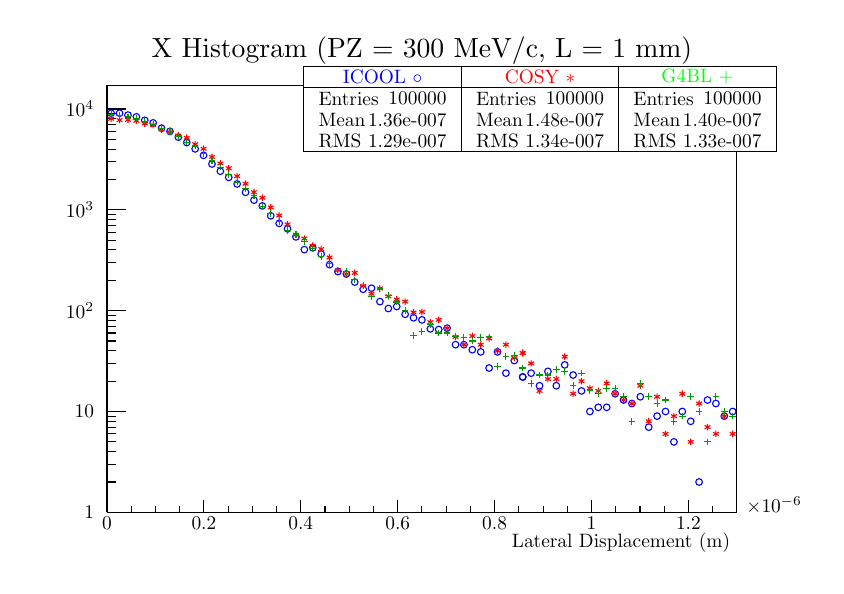
\begin{tikzpicture}
\definecolor{c}{rgb}{1,1,1};
\draw [color=c, fill=c] (0,0) rectangle (20,13.5632);
\draw [color=c, fill=c] (2,1.35632) rectangle (18,12.2069);
\definecolor{c}{rgb}{0,0,0};
\draw [c] (2,1.35632) -- (2,12.2069) -- (18,12.2069) -- (18,1.35632) -- (2,1.35632);
\definecolor{c}{rgb}{1,1,1};
\draw [color=c, fill=c] (2,1.35632) rectangle (18,12.2069);
\definecolor{c}{rgb}{0,0,0};
\draw [c] (2,1.35632) -- (2,12.2069) -- (18,12.2069) -- (18,1.35632) -- (2,1.35632);
\definecolor{c}{rgb}{0,0,1};
\foreach \P in
 {(2.10667,11.4951),(2.32,11.4959),(2.53333,11.4464),(2.74667,11.4024),(2.96,11.3145),(3.17333,11.2482),(3.38667,11.1154),(3.6,11.0343),(3.81333,10.886),(4.02667,10.7495),(4.24,10.5885),(4.45333,10.4245),(4.66667,10.2057),(4.88,10.0219),(5.09333,9.86
533),(5.30667,9.69799),(5.52,9.48538),(5.73333,9.28657),(5.94667,9.13993),(6.16,8.88864),(6.37333,8.69698),(6.58667,8.55663),(6.8,8.35345),(7.01333,8.02997),(7.22667,8.07594),(7.44,7.91674),(7.65333,7.64845),(7.86667,7.47177),(8.08,7.41086),(8.29333,
7.20514),(8.50667,7.02298),(8.72,7.04995),(8.93333,6.70974),(9.14667,6.53372),(9.36,6.58547),(9.57333,6.38669),(9.78667,6.29865),(10,6.24502),(10.2133,6.0172),(10.4267,6.00021),(10.64,6.03393),(10.8533,5.61558),(11.0667,5.61558),(11.28,5.48757),(11.4
933,5.43193),(11.7067,5.02285),(11.92,5.43193),(12.1333,4.89182),(12.3467,5.21186),(12.56,4.79502)}{\draw[mark options={color=c,fill=c},mark size=2.402402pt,mark=o] plot coordinates {\P};}
\foreach \P in
 {(12.56,4.79502),(12.7733,4.89182),(12.9867,4.57178),(13.2,4.93723),(13.4133,4.57178),(13.6267,5.10234),(13.84,4.84447),(14.0533,4.44075),(14.2667,3.91788),(14.48,4.02391),(14.6933,4.02391),(14.9067,4.36895),(15.12,4.20976),(15.3333,4.12071),(15.546
7,4.2922),(15.76,3.52109),(15.9733,3.80067),(16.1867,3.91788),(16.4,3.14678),(16.6133,3.91788),(16.8267,3.66964),(17.04,2.12743),(17.2533,4.20976),(17.4667,4.12071),(17.68,3.80067),(17.8933,3.91788)}{\draw[mark options={color=c,fill=c},mark
 size=2.402402pt,mark=o] plot coordinates {\P};}
\definecolor{c}{rgb}{1,1,1};
\draw [color=c, fill=c] (7,10.5115) rectangle (11,12.6816);
\definecolor{c}{rgb}{0,0,0};
\draw [c] (7,10.5115) -- (11,10.5115);
\draw [c] (11,10.5115) -- (11,12.6816);
\draw [c] (11,12.6816) -- (7,12.6816);
\draw [c] (7,12.6816) -- (7,10.5115);
\draw[color=blue](9,12.4103) node[scale=0.7, rotate=0]{ICOOL $\circ$};
\draw [c] (7,12.1391) -- (11,12.1391);
\draw [anchor= west] (7.2,11.8678) node[scale=0.7, rotate=0]{Entries };
\draw [anchor= east] (10.8,11.8678) node[scale=0.7, rotate=0]{ 100000};
\draw [anchor= west] (7.2,11.3253) node[scale=0.7, rotate=0]{Mean  };
\draw [anchor= east] (10.8,11.3253) node[scale=0.7, rotate=0]{ 1.36e-007};
\draw [anchor= west] (7.2,10.7828) node[scale=0.7, rotate=0]{RMS   };
\draw [anchor= east] (10.8,10.7828) node[scale=0.7, rotate=0]{ 1.29e-007};
\draw [c] (2,1.35632) -- (18,1.35632);
\draw [anchor= east] (18,0.596782) node[scale=0.7, rotate=0]{Lateral Displacement (m)};
\draw [c] (2,1.68184) -- (2,1.35632);
\draw [c] (2.61538,1.51908) -- (2.61538,1.35632);
\draw [c] (3.23077,1.51908) -- (3.23077,1.35632);
\draw [c] (3.84615,1.51908) -- (3.84615,1.35632);
\draw [c] (4.46154,1.68184) -- (4.46154,1.35632);
\draw [c] (5.07692,1.51908) -- (5.07692,1.35632);
\draw [c] (5.69231,1.51908) -- (5.69231,1.35632);
\draw [c] (6.30769,1.51908) -- (6.30769,1.35632);
\draw [c] (6.92308,1.68184) -- (6.92308,1.35632);
\draw [c] (7.53846,1.51908) -- (7.53846,1.35632);
\draw [c] (8.15385,1.51908) -- (8.15385,1.35632);
\draw [c] (8.76923,1.51908) -- (8.76923,1.35632);
\draw [c] (9.38461,1.68184) -- (9.38461,1.35632);
\draw [c] (10,1.51908) -- (10,1.35632);
\draw [c] (10.6154,1.51908) -- (10.6154,1.35632);
\draw [c] (11.2308,1.51908) -- (11.2308,1.35632);
\draw [c] (11.8462,1.68184) -- (11.8462,1.35632);
\draw [c] (12.4615,1.51908) -- (12.4615,1.35632);
\draw [c] (13.0769,1.51908) -- (13.0769,1.35632);
\draw [c] (13.6923,1.51908) -- (13.6923,1.35632);
\draw [c] (14.3077,1.68184) -- (14.3077,1.35632);
\draw [c] (14.9231,1.51908) -- (14.9231,1.35632);
\draw [c] (15.5385,1.51908) -- (15.5385,1.35632);
\draw [c] (16.1538,1.51908) -- (16.1538,1.35632);
\draw [c] (16.7692,1.68184) -- (16.7692,1.35632);
\draw [c] (16.7692,1.68184) -- (16.7692,1.35632);
\draw [c] (17.3846,1.51908) -- (17.3846,1.35632);
\draw [c] (18,1.51908) -- (18,1.35632);
\draw [anchor=base] (2,0.908736) node[scale=0.7, rotate=0]{0};
\draw [anchor=base] (4.46154,0.908736) node[scale=0.7, rotate=0]{0.2};
\draw [anchor=base] (6.92308,0.908736) node[scale=0.7, rotate=0]{0.4};
\draw [anchor=base] (9.38461,0.908736) node[scale=0.7, rotate=0]{0.6};
\draw [anchor=base] (11.8462,0.908736) node[scale=0.7, rotate=0]{0.8};
\draw [anchor=base] (14.3077,0.908736) node[scale=0.7, rotate=0]{1};
\draw [anchor=base] (16.7692,0.908736) node[scale=0.7, rotate=0]{1.2};
\draw [anchor=base west] (18.07,1.35632) node[scale=0.7, rotate=0]{$\times10^{-6}$};
\draw [c] (2,1.35632) -- (2,12.2069);
\draw [c] (2.48,1.35632) -- (2,1.35632);
\draw [anchor= east] (1.844,1.35632) node[scale=0.7, rotate=0]{1};
\draw [c] (2.24,2.12743) -- (2,2.12743);
\draw [c] (2.24,2.5785) -- (2,2.5785);
\draw [c] (2.24,2.89854) -- (2,2.89854);
\draw [c] (2.24,3.14678) -- (2,3.14678);
\draw [c] (2.24,3.34961) -- (2,3.34961);
\draw [c] (2.24,3.52109) -- (2,3.52109);
\draw [c] (2.24,3.66964) -- (2,3.66964);
\draw [c] (2.24,3.80067) -- (2,3.80067);
\draw [c] (2.48,3.91789) -- (2,3.91789);
\draw [anchor= east] (1.844,3.91789) node[scale=0.7, rotate=0]{10};
\draw [c] (2.24,4.68899) -- (2,4.68899);
\draw [c] (2.24,5.14006) -- (2,5.14006);
\draw [c] (2.24,5.4601) -- (2,5.4601);
\draw [c] (2.24,5.70834) -- (2,5.70834);
\draw [c] (2.24,5.91117) -- (2,5.91117);
\draw [c] (2.24,6.08266) -- (2,6.08266);
\draw [c] (2.24,6.23121) -- (2,6.23121);
\draw [c] (2.24,6.36224) -- (2,6.36224);
\draw [c] (2.48,6.47945) -- (2,6.47945);
\draw [anchor= east] (1.844,6.47945) node[scale=0.7, rotate=0]{$10^{2}$};
\draw [c] (2.24,7.25055) -- (2,7.25055);
\draw [c] (2.24,7.70162) -- (2,7.70162);
\draw [c] (2.24,8.02166) -- (2,8.02166);
\draw [c] (2.24,8.2699) -- (2,8.2699);
\draw [c] (2.24,8.47273) -- (2,8.47273);
\draw [c] (2.24,8.64422) -- (2,8.64422);
\draw [c] (2.24,8.79277) -- (2,8.79277);
\draw [c] (2.24,8.9238) -- (2,8.9238);
\draw [c] (2.48,9.04101) -- (2,9.04101);
\draw [anchor= east] (1.844,9.04101) node[scale=0.7, rotate=0]{$10^{3}$};
\draw [c] (2.24,9.81211) -- (2,9.81211);
\draw [c] (2.24,10.2632) -- (2,10.2632);
\draw [c] (2.24,10.5832) -- (2,10.5832);
\draw [c] (2.24,10.8315) -- (2,10.8315);
\draw [c] (2.24,11.0343) -- (2,11.0343);
\draw [c] (2.24,11.2058) -- (2,11.2058);
\draw [c] (2.24,11.3543) -- (2,11.3543);
\draw [c] (2.24,11.4854) -- (2,11.4854);
\draw [c] (2.48,11.6026) -- (2,11.6026);
\draw [anchor= east] (1.844,11.6026) node[scale=0.7, rotate=0]{$10^{4}$};
\definecolor{c}{rgb}{1,1,1};
\draw [color=c, fill=c] (7,10.5115) rectangle (11,12.6816);
\definecolor{c}{rgb}{0,0,0};
\draw [c] (7,10.5115) -- (11,10.5115);
\draw [c] (11,10.5115) -- (11,12.6816);
\draw [c] (11,12.6816) -- (7,12.6816);
\draw [c] (7,12.6816) -- (7,10.5115);
\draw[color=blue](9,12.4103) node[scale=0.7, rotate=0]{ICOOL $\circ$};
\draw [c] (7,12.1391) -- (11,12.1391);
\draw [anchor= west] (7.2,11.8678) node[scale=0.7, rotate=0]{Entries };
\draw [anchor= east] (10.8,11.8678) node[scale=0.7, rotate=0]{ 100000};
\draw [anchor= west] (7.2,11.3253) node[scale=0.7, rotate=0]{Mean  };
\draw [anchor= east] (10.8,11.3253) node[scale=0.7, rotate=0]{ 1.36e-007};
\draw [anchor= west] (7.2,10.7828) node[scale=0.7, rotate=0]{RMS   };
\draw [anchor= east] (10.8,10.7828) node[scale=0.7, rotate=0]{ 1.29e-007};
\draw (10,13.0816) node[scale=1, rotate=0]{X Histogram (PZ = 300 MeV/c, L = 1 mm)};
\definecolor{c}{rgb}{1,0,0};
\foreach \P in
 {(2.10667,11.354),(2.32,11.3189),(2.53333,11.326),(2.74667,11.2998),(2.96,11.2348),(3.17333,11.1911),(3.38667,11.0802),(3.6,11.0167),(3.81333,10.9286),(4.02667,10.8699),(4.24,10.7068),(4.45333,10.5904),(4.66667,10.3829),(4.88,10.2178),(5.09333,10.09
8),(5.30667,9.89515),(5.52,9.70413),(5.73333,9.48762),(5.94667,9.34733),(6.16,9.09951),(6.37333,8.89626),(6.58667,8.67246),(6.8,8.40783),(7.01333,8.30925),(7.22667,8.12769),(7.44,8.04369),(7.65333,7.831),(7.86667,7.50766),(8.08,7.41086),(8.29333,7.43
939),(8.50667,7.10834),(8.72,6.90804),(8.93333,7.04327),(9.14667,6.84579),(9.36,6.76273),(9.57333,6.70974),(9.78667,6.43403),(10,6.44556),(10.2133,6.18868),(10.4267,6.24502),(10.64,6.03393),(10.8533,5.81437),(11.0667,5.61558),(11.28,5.83441),(11.4933
,5.61558),(11.7067,5.77316),(11.92,5.4601),(12.1333,5.61558),(12.3467,5.2793),(12.56,5.40304)}{\draw[mark options={color=c,fill=c},mark size=2.402402pt,mark=asterisk] plot coordinates {\P};}
\foreach \P in
 {(12.56,5.40304),(12.7733,5.14006),(12.9867,4.44075),(13.2,4.74327),(13.4133,4.74327),(13.6267,5.31155),(13.84,4.36895),(14.0533,4.68899),(14.2667,4.50819),(14.48,4.44075),(14.6933,4.63193),(14.9067,4.36895),(15.12,4.20976),(15.3333,4.12071),(15.546
7,4.57178),(15.76,3.66964),(15.9733,4.2922),(16.1867,3.3496),(16.4,3.80067),(16.6133,4.36895),(16.8267,3.14678),(17.04,4.12071),(17.2533,3.52109),(17.4667,3.3496),(17.68,3.80067),(17.8933,3.3496)}{\draw[mark options={color=c,fill=c},mark
 size=2.402402pt,mark=asterisk] plot coordinates {\P};}
\definecolor{c}{rgb}{1,1,1};
\draw [color=c, fill=c] (11,10.5115) rectangle (15,12.6816);
\definecolor{c}{rgb}{0,0,0};
\draw [c] (11,10.5115) -- (15,10.5115);
\draw [c] (15,10.5115) -- (15,12.6816);
\draw [c] (15,12.6816) -- (11,12.6816);
\draw [c] (11,12.6816) -- (11,10.5115);
\draw [color=red](13,12.4103) node[scale=0.7, rotate=0]{COSY $*$};
\draw [c] (11,12.1391) -- (15,12.1391);
\draw [anchor= west] (11.2,11.8678) node[scale=0.7, rotate=0]{Entries };
\draw [anchor= east] (14.8,11.8678) node[scale=0.7, rotate=0]{ 100000};
\draw [anchor= west] (11.2,11.3253) node[scale=0.7, rotate=0]{Mean  };
\draw [anchor= east] (14.8,11.3253) node[scale=0.7, rotate=0]{ 1.48e-007};
\draw [anchor= west] (11.2,10.7828) node[scale=0.7, rotate=0]{RMS   };
\draw [anchor= east] (14.8,10.7828) node[scale=0.7, rotate=0]{ 1.34e-007};
\definecolor{c}{rgb}{1,1,1};
\draw [color=c, fill=c] (11,10.5115) rectangle (15,12.6816);
\definecolor{c}{rgb}{0,0,0};
\draw [c] (11,10.5115) -- (15,10.5115);
\draw [c] (15,10.5115) -- (15,12.6816);
\draw [c] (15,12.6816) -- (11,12.6816);
\draw [c] (11,12.6816) -- (11,10.5115);
\draw [color=red](13,12.4103) node[scale=0.7, rotate=0]{COSY $*$};
\draw [c] (11,12.1391) -- (15,12.1391);
\draw [anchor= west] (11.2,11.8678) node[scale=0.7, rotate=0]{Entries };
\draw [anchor= east] (14.8,11.8678) node[scale=0.7, rotate=0]{ 100000};
\draw [anchor= west] (11.2,11.3253) node[scale=0.7, rotate=0]{Mean  };
\draw [anchor= east] (14.8,11.3253) node[scale=0.7, rotate=0]{ 1.48e-007};
\draw [anchor= west] (11.2,10.7828) node[scale=0.7, rotate=0]{RMS   };
\draw [anchor= east] (14.8,10.7828) node[scale=0.7, rotate=0]{ 1.34e-007};
\definecolor{c}{rgb}{0,0.6,0};
\foreach \P in
 {(2.10667,11.4624),(2.32,11.4462),(2.53333,11.4002),(2.74667,11.3567),(2.96,11.2933),(3.17333,11.2162),(3.38667,11.1089),(3.6,11.025),(3.81333,10.8965),(4.02667,10.7617),(4.24,10.659),(4.45333,10.4725),(4.66667,10.2935),(4.88,10.1252),(5.09333,9.945
12),(5.30667,9.74564),(5.52,9.58249),(5.73333,9.39609),(5.94667,9.12353),(6.16,8.94097),(6.37333,8.743),(6.58667,8.51279),(6.8,8.41761),(7.01333,8.22911),(7.22667,8.05454),(7.44,7.85387),(7.65333,7.68292),(7.86667,7.51645),(8.08,7.48085),(8.29333,7.2
6162),(8.50667,7.11464),(8.72,6.83775),(8.93333,7.02978),(9.14667,6.86954),(9.36,6.70066),(9.57333,6.49051),(9.78667,5.8541),(10,5.94764),(10.2133,6.12934),(10.4267,5.91117),(10.64,5.91117),(10.8533,5.83441),(11.0667,5.79396),(11.28,5.70834),(11.4933
,5.79396),(11.7067,5.81437),(11.92,5.06331),(12.1333,5.31155),(12.3467,5.34289),(12.56,5.02285)}{\draw[mark options={color=c,fill=c},mark size=2.402402pt,mark=+] plot coordinates {\P};}
\foreach \P in
 {(12.56,5.02285),(12.7733,4.63193),(12.9867,4.84447),(13.2,4.84447),(13.4133,4.98086),(13.6267,4.93723),(13.84,4.57178),(14.0533,4.89182),(14.2667,4.44075),(14.48,4.36895),(14.6933,4.50819),(14.9067,4.50819),(15.12,4.2922),(15.3333,3.66964),(15.5467
,4.63193),(15.76,4.2922),(15.9733,4.12071),(16.1867,4.20976),(16.4,3.66964),(16.6133,3.80067),(16.8267,4.2922),(17.04,3.91788),(17.2533,3.14678),(17.4667,4.2922),(17.68,3.91788),(17.8933,3.80067)}{\draw[mark options={color=c,fill=c},mark
 size=2.402402pt,mark=+] plot coordinates {\P};}
\definecolor{c}{rgb}{1,1,1};
\draw [color=c, fill=c] (15,10.5115) rectangle (19,12.6816);
\definecolor{c}{rgb}{0,0,0};
\draw [c] (15,10.5115) -- (19,10.5115);
\draw [c] (19,10.5115) -- (19,12.6816);
\draw [c] (19,12.6816) -- (15,12.6816);
\draw [c] (15,12.6816) -- (15,10.5115);
\draw [color=green](17,12.4103) node[scale=0.7, rotate=0]{G4BL $+$};
\draw [c] (15,12.1391) -- (19,12.1391);
\draw [anchor= west] (15.2,11.8678) node[scale=0.7, rotate=0]{Entries };
\draw [anchor= east] (18.8,11.8678) node[scale=0.7, rotate=0]{ 100000};
\draw [anchor= west] (15.2,11.3253) node[scale=0.7, rotate=0]{Mean  };
\draw [anchor= east] (18.8,11.3253) node[scale=0.7, rotate=0]{ 1.40e-007};
\draw [anchor= west] (15.2,10.7828) node[scale=0.7, rotate=0]{RMS   };
\draw [anchor= east] (18.8,10.7828) node[scale=0.7, rotate=0]{ 1.33e-007};
\definecolor{c}{rgb}{1,1,1};
\draw [color=c, fill=c] (15,10.5115) rectangle (19,12.6816);
\definecolor{c}{rgb}{0,0,0};
\draw [c] (15,10.5115) -- (19,10.5115);
\draw [c] (19,10.5115) -- (19,12.6816);
\draw [c] (19,12.6816) -- (15,12.6816);
\draw [c] (15,12.6816) -- (15,10.5115);
\draw [color=green](17,12.4103) node[scale=0.7, rotate=0]{G4BL $+$};
\draw [c] (15,12.1391) -- (19,12.1391);
\draw [anchor= west] (15.2,11.8678) node[scale=0.7, rotate=0]{Entries };
\draw [anchor= east] (18.8,11.8678) node[scale=0.7, rotate=0]{ 100000};
\draw [anchor= west] (15.2,11.3253) node[scale=0.7, rotate=0]{Mean  };
\draw [anchor= east] (18.8,11.3253) node[scale=0.7, rotate=0]{ 1.40e-007};
\draw [anchor= west] (15.2,10.7828) node[scale=0.7, rotate=0]{RMS   };
\draw [anchor= east] (18.8,10.7828) node[scale=0.7, rotate=0]{ 1.33e-007};
\end{tikzpicture}
}\\
\frame{    \pgfdeclareplotmark{cross} {
\pgfpathmoveto{\pgfpoint{-0.3\pgfplotmarksize}{\pgfplotmarksize}}
\pgfpathlineto{\pgfpoint{+0.3\pgfplotmarksize}{\pgfplotmarksize}}
\pgfpathlineto{\pgfpoint{+0.3\pgfplotmarksize}{0.3\pgfplotmarksize}}
\pgfpathlineto{\pgfpoint{+1\pgfplotmarksize}{0.3\pgfplotmarksize}}
\pgfpathlineto{\pgfpoint{+1\pgfplotmarksize}{-0.3\pgfplotmarksize}}
\pgfpathlineto{\pgfpoint{+0.3\pgfplotmarksize}{-0.3\pgfplotmarksize}}
\pgfpathlineto{\pgfpoint{+0.3\pgfplotmarksize}{-1.\pgfplotmarksize}}
\pgfpathlineto{\pgfpoint{-0.3\pgfplotmarksize}{-1.\pgfplotmarksize}}
\pgfpathlineto{\pgfpoint{-0.3\pgfplotmarksize}{-0.3\pgfplotmarksize}}
\pgfpathlineto{\pgfpoint{-1.\pgfplotmarksize}{-0.3\pgfplotmarksize}}
\pgfpathlineto{\pgfpoint{-1.\pgfplotmarksize}{0.3\pgfplotmarksize}}
\pgfpathlineto{\pgfpoint{-0.3\pgfplotmarksize}{0.3\pgfplotmarksize}}
\pgfpathclose
\pgfusepathqstroke
}
\pgfdeclareplotmark{cross*} {
\pgfpathmoveto{\pgfpoint{-0.3\pgfplotmarksize}{\pgfplotmarksize}}
\pgfpathlineto{\pgfpoint{+0.3\pgfplotmarksize}{\pgfplotmarksize}}
\pgfpathlineto{\pgfpoint{+0.3\pgfplotmarksize}{0.3\pgfplotmarksize}}
\pgfpathlineto{\pgfpoint{+1\pgfplotmarksize}{0.3\pgfplotmarksize}}
\pgfpathlineto{\pgfpoint{+1\pgfplotmarksize}{-0.3\pgfplotmarksize}}
\pgfpathlineto{\pgfpoint{+0.3\pgfplotmarksize}{-0.3\pgfplotmarksize}}
\pgfpathlineto{\pgfpoint{+0.3\pgfplotmarksize}{-1.\pgfplotmarksize}}
\pgfpathlineto{\pgfpoint{-0.3\pgfplotmarksize}{-1.\pgfplotmarksize}}
\pgfpathlineto{\pgfpoint{-0.3\pgfplotmarksize}{-0.3\pgfplotmarksize}}
\pgfpathlineto{\pgfpoint{-1.\pgfplotmarksize}{-0.3\pgfplotmarksize}}
\pgfpathlineto{\pgfpoint{-1.\pgfplotmarksize}{0.3\pgfplotmarksize}}
\pgfpathlineto{\pgfpoint{-0.3\pgfplotmarksize}{0.3\pgfplotmarksize}}
\pgfpathclose
\pgfusepathqfillstroke
}
\pgfdeclareplotmark{newstar} {
\pgfpathmoveto{\pgfqpoint{0pt}{\pgfplotmarksize}}
\pgfpathlineto{\pgfqpointpolar{44}{0.5\pgfplotmarksize}}
\pgfpathlineto{\pgfqpointpolar{18}{\pgfplotmarksize}}
\pgfpathlineto{\pgfqpointpolar{-20}{0.5\pgfplotmarksize}}
\pgfpathlineto{\pgfqpointpolar{-54}{\pgfplotmarksize}}
\pgfpathlineto{\pgfqpointpolar{-90}{0.5\pgfplotmarksize}}
\pgfpathlineto{\pgfqpointpolar{234}{\pgfplotmarksize}}
\pgfpathlineto{\pgfqpointpolar{198}{0.5\pgfplotmarksize}}
\pgfpathlineto{\pgfqpointpolar{162}{\pgfplotmarksize}}
\pgfpathlineto{\pgfqpointpolar{134}{0.5\pgfplotmarksize}}
\pgfpathclose
\pgfusepathqstroke
}
\pgfdeclareplotmark{newstar*} {
\pgfpathmoveto{\pgfqpoint{0pt}{\pgfplotmarksize}}
\pgfpathlineto{\pgfqpointpolar{44}{0.5\pgfplotmarksize}}
\pgfpathlineto{\pgfqpointpolar{18}{\pgfplotmarksize}}
\pgfpathlineto{\pgfqpointpolar{-20}{0.5\pgfplotmarksize}}
\pgfpathlineto{\pgfqpointpolar{-54}{\pgfplotmarksize}}
\pgfpathlineto{\pgfqpointpolar{-90}{0.5\pgfplotmarksize}}
\pgfpathlineto{\pgfqpointpolar{234}{\pgfplotmarksize}}
\pgfpathlineto{\pgfqpointpolar{198}{0.5\pgfplotmarksize}}
\pgfpathlineto{\pgfqpointpolar{162}{\pgfplotmarksize}}
\pgfpathlineto{\pgfqpointpolar{134}{0.5\pgfplotmarksize}}
\pgfpathclose
\pgfusepathqfillstroke
}
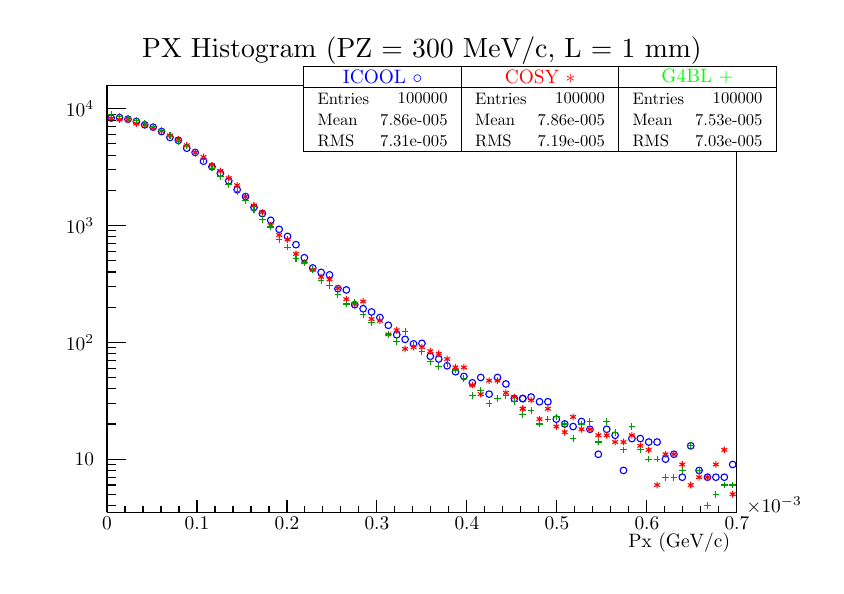
\begin{tikzpicture}
\definecolor{c}{rgb}{1,1,1};
\draw [color=c, fill=c] (0,0) rectangle (20,13.5632);
\draw [color=c, fill=c] (2,1.35632) rectangle (18,12.2069);
\definecolor{c}{rgb}{0,0,0};
\draw [c] (2,1.35632) -- (2,12.2069) -- (18,12.2069) -- (18,1.35632) -- (2,1.35632);
\definecolor{c}{rgb}{1,1,1};
\draw [color=c, fill=c] (2,1.35632) rectangle (18,12.2069);
\definecolor{c}{rgb}{0,0,0};
\draw [c] (2,1.35632) -- (2,12.2069) -- (18,12.2069) -- (18,1.35632) -- (2,1.35632);
\definecolor{c}{rgb}{0,0,1};
\foreach \P in
 {(2.10667,11.3716),(2.32,11.3836),(2.53333,11.3406),(2.74667,11.2842),(2.96,11.1998),(3.17333,11.1393),(3.38667,11.0287),(3.6,10.8797),(3.81333,10.805),(4.02667,10.6067),(4.24,10.4983),(4.45333,10.2759),(4.66667,10.1351),(4.88,9.9698),(5.09333,9.775
8),(5.30667,9.5524),(5.52,9.37783),(5.73333,9.1005),(5.94667,8.94538),(6.16,8.77481),(6.37333,8.54387),(6.58667,8.36528),(6.8,8.156),(7.01333,7.82362),(7.22667,7.56321),(7.44,7.45139),(7.65333,7.38821),(7.86667,7.03788),(8.08,7.00618),(8.29333,6.6309
8),(8.50667,6.52888),(8.72,6.44662),(8.93333,6.30458),(9.14667,6.10862),(9.36,5.86636),(9.57333,5.75022),(9.78667,5.63591),(10,5.64913),(10.2133,5.3216),(10.4267,5.25195),(10.64,5.07992),(10.8533,4.92819),(11.0667,4.8077),(11.28,4.64645),(11.4933,4.7
8219),(11.7067,4.35898),(11.92,4.78219),(12.1333,4.6175),(12.3467,4.24689),(12.56,4.24689)}{\draw[mark options={color=c,fill=c},mark size=2.402402pt,mark=o] plot coordinates {\P};}
\foreach \P in
 {(12.56,4.24689),(12.7733,4.28535),(12.9867,4.16634),(13.2,4.16634),(13.4133,3.72454),(13.6267,3.60175),(13.84,3.53567),(14.0533,3.66461),(14.2667,3.46602),(14.48,2.83157),(14.6933,3.46602),(14.9067,3.31428),(15.12,2.42131),(15.3333,3.23114),(15.546
7,3.23114),(15.76,3.14225),(15.9733,3.14225),(16.1867,2.70878),(16.4,2.83157),(16.6133,2.24929),(16.8267,3.04678),(17.04,2.42131),(17.2533,2.24929),(17.4667,2.24929),(17.68,2.24929),(17.8933,2.57305)}{\draw[mark options={color=c,fill=c},mark
 size=2.402402pt,mark=o] plot coordinates {\P};}
\definecolor{c}{rgb}{1,1,1};
\draw [color=c, fill=c] (7,10.5115) rectangle (11,12.6816);
\definecolor{c}{rgb}{0,0,0};
\draw [c] (7,10.5115) -- (11,10.5115);
\draw [c] (11,10.5115) -- (11,12.6816);
\draw [c] (11,12.6816) -- (7,12.6816);
\draw [c] (7,12.6816) -- (7,10.5115);
\draw[color=blue](9,12.4103) node[scale=0.7, rotate=0]{ICOOL $\circ$};
\draw [c] (7,12.1391) -- (11,12.1391);
\draw [anchor= west] (7.2,11.8678) node[scale=0.6, rotate=0]{Entries };
\draw [anchor= east] (10.8,11.8678) node[scale=0.6, rotate=0]{ 100000};
\draw [anchor= west] (7.2,11.3253) node[scale=0.6, rotate=0]{Mean  };
\draw [anchor= east] (10.8,11.3253) node[scale=0.6, rotate=0]{ 7.86e-005};
\draw [anchor= west] (7.2,10.7828) node[scale=0.6, rotate=0]{RMS   };
\draw [anchor= east] (10.8,10.7828) node[scale=0.6, rotate=0]{ 7.31e-005};
\draw [c] (2,1.35632) -- (18,1.35632);
\draw [anchor= east] (18,0.596782) node[scale=0.7, rotate=0]{Px (GeV/c)};
\draw [c] (2,1.68184) -- (2,1.35632);
\draw [c] (2.45714,1.51908) -- (2.45714,1.35632);
\draw [c] (2.91429,1.51908) -- (2.91429,1.35632);
\draw [c] (3.37143,1.51908) -- (3.37143,1.35632);
\draw [c] (3.82857,1.51908) -- (3.82857,1.35632);
\draw [c] (4.28571,1.68184) -- (4.28571,1.35632);
\draw [c] (4.74286,1.51908) -- (4.74286,1.35632);
\draw [c] (5.2,1.51908) -- (5.2,1.35632);
\draw [c] (5.65714,1.51908) -- (5.65714,1.35632);
\draw [c] (6.11429,1.51908) -- (6.11429,1.35632);
\draw [c] (6.57143,1.68184) -- (6.57143,1.35632);
\draw [c] (7.02857,1.51908) -- (7.02857,1.35632);
\draw [c] (7.48571,1.51908) -- (7.48571,1.35632);
\draw [c] (7.94286,1.51908) -- (7.94286,1.35632);
\draw [c] (8.4,1.51908) -- (8.4,1.35632);
\draw [c] (8.85714,1.68184) -- (8.85714,1.35632);
\draw [c] (9.31429,1.51908) -- (9.31429,1.35632);
\draw [c] (9.77143,1.51908) -- (9.77143,1.35632);
\draw [c] (10.2286,1.51908) -- (10.2286,1.35632);
\draw [c] (10.6857,1.51908) -- (10.6857,1.35632);
\draw [c] (11.1429,1.68184) -- (11.1429,1.35632);
\draw [c] (11.6,1.51908) -- (11.6,1.35632);
\draw [c] (12.0571,1.51908) -- (12.0571,1.35632);
\draw [c] (12.5143,1.51908) -- (12.5143,1.35632);
\draw [c] (12.9714,1.51908) -- (12.9714,1.35632);
\draw [c] (13.4286,1.68184) -- (13.4286,1.35632);
\draw [c] (13.8857,1.51908) -- (13.8857,1.35632);
\draw [c] (14.3429,1.51908) -- (14.3429,1.35632);
\draw [c] (14.8,1.51908) -- (14.8,1.35632);
\draw [c] (15.2571,1.51908) -- (15.2571,1.35632);
\draw [c] (15.7143,1.68184) -- (15.7143,1.35632);
\draw [c] (16.1714,1.51908) -- (16.1714,1.35632);
\draw [c] (16.6286,1.51908) -- (16.6286,1.35632);
\draw [c] (17.0857,1.51908) -- (17.0857,1.35632);
\draw [c] (17.5429,1.51908) -- (17.5429,1.35632);
\draw [c] (18,1.68184) -- (18,1.35632);
\draw [c] (18,1.68184) -- (18,1.35632);
\draw [anchor=base] (2,0.908736) node[scale=0.7, rotate=0]{0};
\draw [anchor=base] (4.28571,0.908736) node[scale=0.7, rotate=0]{0.1};
\draw [anchor=base] (6.57143,0.908736) node[scale=0.7, rotate=0]{0.2};
\draw [anchor=base] (8.85714,0.908736) node[scale=0.7, rotate=0]{0.3};
\draw [anchor=base] (11.1429,0.908736) node[scale=0.7, rotate=0]{0.4};
\draw [anchor=base] (13.4286,0.908736) node[scale=0.7, rotate=0]{0.5};
\draw [anchor=base] (15.7143,0.908736) node[scale=0.7, rotate=0]{0.6};
\draw [anchor=base] (18,0.908736) node[scale=0.7, rotate=0]{0.7};
\draw [anchor=base west] (18.07,1.35632) node[scale=0.7, rotate=0]{$\times10^{-3}$};
\draw [c] (2,1.35632) -- (2,12.2069);
\draw [c] (2.24,1.52834) -- (2,1.52834);
\draw [c] (2.24,1.81582) -- (2,1.81582);
\draw [c] (2.24,2.0507) -- (2,2.0507);
\draw [c] (2.24,2.24929) -- (2,2.24929);
\draw [c] (2.24,2.42131) -- (2,2.42131);
\draw [c] (2.24,2.57305) -- (2,2.57305);
\draw [c] (2.48,2.70878) -- (2,2.70878);
\draw [anchor= east] (1.844,2.70878) node[scale=0.7, rotate=0]{10};
\draw [c] (2.24,3.60175) -- (2,3.60175);
\draw [c] (2.24,4.1241) -- (2,4.1241);
\draw [c] (2.24,4.49471) -- (2,4.49471);
\draw [c] (2.24,4.78219) -- (2,4.78219);
\draw [c] (2.24,5.01707) -- (2,5.01707);
\draw [c] (2.24,5.21566) -- (2,5.21566);
\draw [c] (2.24,5.38768) -- (2,5.38768);
\draw [c] (2.24,5.53942) -- (2,5.53942);
\draw [c] (2.48,5.67515) -- (2,5.67515);
\draw [anchor= east] (1.844,5.67515) node[scale=0.7, rotate=0]{$10^{2}$};
\draw [c] (2.24,6.56812) -- (2,6.56812);
\draw [c] (2.24,7.09047) -- (2,7.09047);
\draw [c] (2.24,7.46108) -- (2,7.46108);
\draw [c] (2.24,7.74856) -- (2,7.74856);
\draw [c] (2.24,7.98344) -- (2,7.98344);
\draw [c] (2.24,8.18203) -- (2,8.18203);
\draw [c] (2.24,8.35405) -- (2,8.35405);
\draw [c] (2.24,8.50579) -- (2,8.50579);
\draw [c] (2.48,8.64152) -- (2,8.64152);
\draw [anchor= east] (1.844,8.64152) node[scale=0.7, rotate=0]{$10^{3}$};
\draw [c] (2.24,9.53449) -- (2,9.53449);
\draw [c] (2.24,10.0568) -- (2,10.0568);
\draw [c] (2.24,10.4275) -- (2,10.4275);
\draw [c] (2.24,10.7149) -- (2,10.7149);
\draw [c] (2.24,10.9498) -- (2,10.9498);
\draw [c] (2.24,11.1484) -- (2,11.1484);
\draw [c] (2.24,11.3204) -- (2,11.3204);
\draw [c] (2.24,11.4722) -- (2,11.4722);
\draw [c] (2.48,11.6079) -- (2,11.6079);
\draw [anchor= east] (1.844,11.6079) node[scale=0.7, rotate=0]{$10^{4}$};
\definecolor{c}{rgb}{1,1,1};
\draw [color=c, fill=c] (7,10.5115) rectangle (11,12.6816);
\definecolor{c}{rgb}{0,0,0};
\draw [c] (7,10.5115) -- (11,10.5115);
\draw [c] (11,10.5115) -- (11,12.6816);
\draw [c] (11,12.6816) -- (7,12.6816);
\draw [c] (7,12.6816) -- (7,10.5115);
\draw[color=blue](9,12.4103) node[scale=0.7, rotate=0]{ICOOL $\circ$};
\draw [c] (7,12.1391) -- (11,12.1391);
\draw [anchor= west] (7.2,11.8678) node[scale=0.6, rotate=0]{Entries };
\draw [anchor= east] (10.8,11.8678) node[scale=0.6, rotate=0]{ 100000};
\draw [anchor= west] (7.2,11.3253) node[scale=0.6, rotate=0]{Mean  };
\draw [anchor= east] (10.8,11.3253) node[scale=0.6, rotate=0]{ 7.86e-005};
\draw [anchor= west] (7.2,10.7828) node[scale=0.6, rotate=0]{RMS   };
\draw [anchor= east] (10.8,10.7828) node[scale=0.6, rotate=0]{ 7.31e-005};
\draw (10,13.0816) node[scale=1, rotate=0]{PX Histogram (PZ = 300 MeV/c, L = 1 mm)};
\definecolor{c}{rgb}{1,0,0};
\foreach \P in
 {(2.10667,11.3601),(2.32,11.3316),(2.53333,11.3326),(2.74667,11.229),(2.96,11.195),(3.17333,11.1224),(3.38667,11.042),(3.6,10.9319),(3.81333,10.8314),(4.02667,10.6805),(4.24,10.4992),(4.45333,10.3819),(4.66667,10.1765),(4.88,10.0286),(5.09333,9.8459
5),(5.30667,9.66428),(5.52,9.37492),(5.73333,9.14919),(5.94667,8.97853),(6.16,8.65179),(6.37333,8.39993),(6.58667,8.28797),(6.8,7.92187),(7.01333,7.70666),(7.22667,7.51779),(7.44,7.33604),(7.65333,7.27425),(7.86667,7.0468),(8.08,6.77038),(8.29333,6.6
4925),(8.50667,6.71412),(8.72,6.26444),(8.93333,6.22302),(9.14667,5.87742),(9.36,5.98307),(9.57333,5.51047),(9.78667,5.55366),(10,5.55366),(10.2133,5.45054),(10.4267,5.38768),(10.64,5.25195),(10.8533,5.03836),(11.0667,5.03836),(11.28,4.58789),(11.493
3,4.35898),(11.7067,4.70248),(11.92,4.70248),(12.1333,4.39428),(12.3467,4.28535),(12.56,3.98837)}{\draw[mark options={color=c,fill=c},mark size=2.402402pt,mark=asterisk] plot coordinates {\P};}
\foreach \P in
 {(12.56,3.98837),(12.7733,4.20725),(12.9867,3.72454),(13.2,3.98837),(13.4133,3.53567),(13.6267,3.39238),(13.84,3.7818),(14.0533,3.46602),(14.2667,3.46602),(14.48,3.31428),(14.6933,3.31428),(14.9067,3.14225),(15.12,3.14225),(15.3333,3.31428),(15.5467
,3.04678),(15.76,2.94367),(15.9733,2.0507),(16.1867,2.83157),(16.4,2.83157),(16.6133,2.57305),(16.8267,2.0507),(17.04,2.24929),(17.2533,2.24929),(17.4667,2.57305),(17.68,2.94367),(17.8933,1.81582)}{\draw[mark options={color=c,fill=c},mark
 size=2.402402pt,mark=asterisk] plot coordinates {\P};}
\definecolor{c}{rgb}{1,1,1};
\draw [color=c, fill=c] (11,10.5115) rectangle (15,12.6816);
\definecolor{c}{rgb}{0,0,0};
\draw [c] (11,10.5115) -- (15,10.5115);
\draw [c] (15,10.5115) -- (15,12.6816);
\draw [c] (15,12.6816) -- (11,12.6816);
\draw [c] (11,12.6816) -- (11,10.5115);
\draw [color=red](13,12.4103) node[scale=0.7, rotate=0]{COSY $*$};
\draw [c] (11,12.1391) -- (15,12.1391);
\draw [anchor= west] (11.2,11.8678) node[scale=0.6, rotate=0]{Entries };
\draw [anchor= east] (14.8,11.8678) node[scale=0.6, rotate=0]{ 100000};
\draw [anchor= west] (11.2,11.3253) node[scale=0.6, rotate=0]{Mean  };
\draw [anchor= east] (14.8,11.3253) node[scale=0.6, rotate=0]{ 7.86e-005};
\draw [anchor= west] (11.2,10.7828) node[scale=0.6, rotate=0]{RMS   };
\draw [anchor= east] (14.8,10.7828) node[scale=0.6, rotate=0]{ 7.19e-005};
\definecolor{c}{rgb}{1,1,1};
\draw [color=c, fill=c] (11,10.5115) rectangle (15,12.6816);
\definecolor{c}{rgb}{0,0,0};
\draw [c] (11,10.5115) -- (15,10.5115);
\draw [c] (15,10.5115) -- (15,12.6816);
\draw [c] (15,12.6816) -- (11,12.6816);
\draw [c] (11,12.6816) -- (11,10.5115);
\draw [color=red](13,12.4103) node[scale=0.7, rotate=0]{COSY $*$};
\draw [c] (11,12.1391) -- (15,12.1391);
\draw [anchor= west] (11.2,11.8678) node[scale=0.6, rotate=0]{Entries };
\draw [anchor= east] (14.8,11.8678) node[scale=0.6, rotate=0]{ 100000};
\draw [anchor= west] (11.2,11.3253) node[scale=0.6, rotate=0]{Mean  };
\draw [anchor= east] (14.8,11.3253) node[scale=0.6, rotate=0]{ 7.86e-005};
\draw [anchor= west] (11.2,10.7828) node[scale=0.6, rotate=0]{RMS   };
\draw [anchor= east] (14.8,10.7828) node[scale=0.6, rotate=0]{ 7.19e-005};
\definecolor{c}{rgb}{0,0.6,0};
\foreach \P in
 {(2.10667,11.4582),(2.32,11.4092),(2.53333,11.3757),(2.74667,11.3156),(2.96,11.2373),(3.17333,11.1565),(3.38667,11.0663),(3.6,10.9209),(3.81333,10.7822),(4.02667,10.6656),(4.24,10.4749),(4.45333,10.3242),(4.66667,10.1012),(4.88,9.89313),(5.09333,9.6
7299),(5.30667,9.4979),(5.52,9.27961),(5.73333,9.05084),(5.94667,8.79897),(6.16,8.60361),(6.37333,8.28967),(6.58667,8.09446),(6.8,7.79908),(7.01333,7.70932),(7.22667,7.51779),(7.44,7.25172),(7.65333,7.12019),(7.86667,6.8811),(8.08,6.64925),(8.29333,6
.68504),(8.50667,6.38871),(8.72,6.17148),(8.93333,6.26444),(9.14667,5.87742),(9.36,5.70066),(9.57333,5.95228),(9.78667,5.59544),(10,5.43511),(10.2133,5.17831),(10.4267,5.05931),(10.64,5.13985),(10.8533,4.97339),(11.0667,4.75616),(11.28,4.32269),(11.4
933,4.4621),(11.7067,4.1241),(11.92,4.24689),(12.1333,4.32269),(12.3467,4.16634),(12.56,3.83663)}{\draw[mark options={color=c,fill=c},mark size=2.402402pt,mark=+] plot coordinates {\P};}
\foreach \P in
 {(12.56,3.83663),(12.7733,3.93975),(12.9867,3.60175),(13.2,3.72454),(13.4133,3.7818),(13.6267,3.60175),(13.84,3.23114),(14.0533,3.60175),(14.2667,3.66461),(14.48,3.14225),(14.6933,3.66461),(14.9067,3.39238),(15.12,2.94367),(15.3333,3.53567),(15.5467
,2.94367),(15.76,2.70878),(15.9733,2.70878),(16.1867,2.24929),(16.4,2.24929),(16.6133,2.42131),(16.8267,3.04678),(17.04,2.42131),(17.2533,1.52835),(17.4667,1.81582),(17.68,2.0507),(17.8933,2.0507)}{\draw[mark options={color=c,fill=c},mark
 size=2.402402pt,mark=+] plot coordinates {\P};}
\definecolor{c}{rgb}{1,1,1};
\draw [color=c, fill=c] (15,10.5115) rectangle (19,12.6816);
\definecolor{c}{rgb}{0,0,0};
\draw [c] (15,10.5115) -- (19,10.5115);
\draw [c] (19,10.5115) -- (19,12.6816);
\draw [c] (19,12.6816) -- (15,12.6816);
\draw [c] (15,12.6816) -- (15,10.5115);
\draw [color=green](17,12.4103) node[scale=0.7, rotate=0]{G4BL $+$};
\draw [c] (15,12.1391) -- (19,12.1391);
\draw [anchor= west] (15.2,11.8678) node[scale=0.6, rotate=0]{Entries };
\draw [anchor= east] (18.8,11.8678) node[scale=0.6, rotate=0]{ 100000};
\draw [anchor= west] (15.2,11.3253) node[scale=0.6, rotate=0]{Mean  };
\draw [anchor= east] (18.8,11.3253) node[scale=0.6, rotate=0]{ 7.53e-005};
\draw [anchor= west] (15.2,10.7828) node[scale=0.6, rotate=0]{RMS   };
\draw [anchor= east] (18.8,10.7828) node[scale=0.6, rotate=0]{ 7.03e-005};
\definecolor{c}{rgb}{1,1,1};
\draw [color=c, fill=c] (15,10.5115) rectangle (19,12.6816);
\definecolor{c}{rgb}{0,0,0};
\draw [c] (15,10.5115) -- (19,10.5115);
\draw [c] (19,10.5115) -- (19,12.6816);
\draw [c] (19,12.6816) -- (15,12.6816);
\draw [c] (15,12.6816) -- (15,10.5115);
\draw [color=green](17,12.4103) node[scale=0.7, rotate=0]{G4BL $+$};
\draw [c] (15,12.1391) -- (19,12.1391);
\draw [anchor= west] (15.2,11.8678) node[scale=0.6, rotate=0]{Entries };
\draw [anchor= east] (18.8,11.8678) node[scale=0.6, rotate=0]{ 100000};
\draw [anchor= west] (15.2,11.3253) node[scale=0.6, rotate=0]{Mean  };
\draw [anchor= east] (18.8,11.3253) node[scale=0.6, rotate=0]{ 7.53e-005};
\draw [anchor= west] (15.2,10.7828) node[scale=0.6, rotate=0]{RMS   };
\draw [anchor= east] (18.8,10.7828) node[scale=0.6, rotate=0]{ 7.03e-005};
\end{tikzpicture}
}\\
\frame{\pgfdeclareplotmark{cross} {
\pgfpathmoveto{\pgfpoint{-0.3\pgfplotmarksize}{\pgfplotmarksize}}
\pgfpathlineto{\pgfpoint{+0.3\pgfplotmarksize}{\pgfplotmarksize}}
\pgfpathlineto{\pgfpoint{+0.3\pgfplotmarksize}{0.3\pgfplotmarksize}}
\pgfpathlineto{\pgfpoint{+1\pgfplotmarksize}{0.3\pgfplotmarksize}}
\pgfpathlineto{\pgfpoint{+1\pgfplotmarksize}{-0.3\pgfplotmarksize}}
\pgfpathlineto{\pgfpoint{+0.3\pgfplotmarksize}{-0.3\pgfplotmarksize}}
\pgfpathlineto{\pgfpoint{+0.3\pgfplotmarksize}{-1.\pgfplotmarksize}}
\pgfpathlineto{\pgfpoint{-0.3\pgfplotmarksize}{-1.\pgfplotmarksize}}
\pgfpathlineto{\pgfpoint{-0.3\pgfplotmarksize}{-0.3\pgfplotmarksize}}
\pgfpathlineto{\pgfpoint{-1.\pgfplotmarksize}{-0.3\pgfplotmarksize}}
\pgfpathlineto{\pgfpoint{-1.\pgfplotmarksize}{0.3\pgfplotmarksize}}
\pgfpathlineto{\pgfpoint{-0.3\pgfplotmarksize}{0.3\pgfplotmarksize}}
\pgfpathclose
\pgfusepathqstroke
}
\pgfdeclareplotmark{cross*} {
\pgfpathmoveto{\pgfpoint{-0.3\pgfplotmarksize}{\pgfplotmarksize}}
\pgfpathlineto{\pgfpoint{+0.3\pgfplotmarksize}{\pgfplotmarksize}}
\pgfpathlineto{\pgfpoint{+0.3\pgfplotmarksize}{0.3\pgfplotmarksize}}
\pgfpathlineto{\pgfpoint{+1\pgfplotmarksize}{0.3\pgfplotmarksize}}
\pgfpathlineto{\pgfpoint{+1\pgfplotmarksize}{-0.3\pgfplotmarksize}}
\pgfpathlineto{\pgfpoint{+0.3\pgfplotmarksize}{-0.3\pgfplotmarksize}}
\pgfpathlineto{\pgfpoint{+0.3\pgfplotmarksize}{-1.\pgfplotmarksize}}
\pgfpathlineto{\pgfpoint{-0.3\pgfplotmarksize}{-1.\pgfplotmarksize}}
\pgfpathlineto{\pgfpoint{-0.3\pgfplotmarksize}{-0.3\pgfplotmarksize}}
\pgfpathlineto{\pgfpoint{-1.\pgfplotmarksize}{-0.3\pgfplotmarksize}}
\pgfpathlineto{\pgfpoint{-1.\pgfplotmarksize}{0.3\pgfplotmarksize}}
\pgfpathlineto{\pgfpoint{-0.3\pgfplotmarksize}{0.3\pgfplotmarksize}}
\pgfpathclose
\pgfusepathqfillstroke
}
\pgfdeclareplotmark{newstar} {
\pgfpathmoveto{\pgfqpoint{0pt}{\pgfplotmarksize}}
\pgfpathlineto{\pgfqpointpolar{44}{0.5\pgfplotmarksize}}
\pgfpathlineto{\pgfqpointpolar{18}{\pgfplotmarksize}}
\pgfpathlineto{\pgfqpointpolar{-20}{0.5\pgfplotmarksize}}
\pgfpathlineto{\pgfqpointpolar{-54}{\pgfplotmarksize}}
\pgfpathlineto{\pgfqpointpolar{-90}{0.5\pgfplotmarksize}}
\pgfpathlineto{\pgfqpointpolar{234}{\pgfplotmarksize}}
\pgfpathlineto{\pgfqpointpolar{198}{0.5\pgfplotmarksize}}
\pgfpathlineto{\pgfqpointpolar{162}{\pgfplotmarksize}}
\pgfpathlineto{\pgfqpointpolar{134}{0.5\pgfplotmarksize}}
\pgfpathclose
\pgfusepathqstroke
}
\pgfdeclareplotmark{newstar*} {
\pgfpathmoveto{\pgfqpoint{0pt}{\pgfplotmarksize}}
\pgfpathlineto{\pgfqpointpolar{44}{0.5\pgfplotmarksize}}
\pgfpathlineto{\pgfqpointpolar{18}{\pgfplotmarksize}}
\pgfpathlineto{\pgfqpointpolar{-20}{0.5\pgfplotmarksize}}
\pgfpathlineto{\pgfqpointpolar{-54}{\pgfplotmarksize}}
\pgfpathlineto{\pgfqpointpolar{-90}{0.5\pgfplotmarksize}}
\pgfpathlineto{\pgfqpointpolar{234}{\pgfplotmarksize}}
\pgfpathlineto{\pgfqpointpolar{198}{0.5\pgfplotmarksize}}
\pgfpathlineto{\pgfqpointpolar{162}{\pgfplotmarksize}}
\pgfpathlineto{\pgfqpointpolar{134}{0.5\pgfplotmarksize}}
\pgfpathclose
\pgfusepathqfillstroke
}
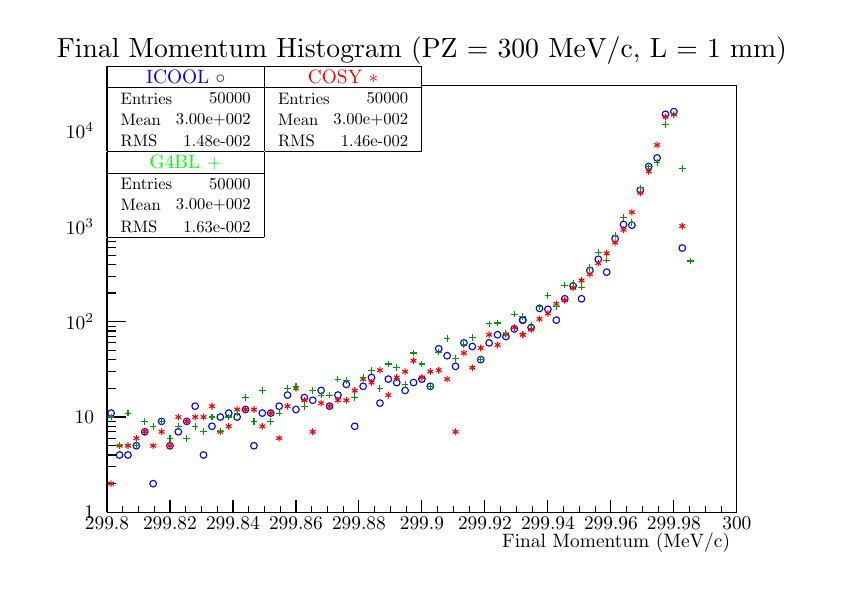
\begin{tikzpicture}
\definecolor{c}{rgb}{1,1,1};
\draw [color=c, fill=c] (0,0) rectangle (20,13.5632);
\draw [color=c, fill=c] (2,1.35632) rectangle (18,12.2069);
\definecolor{c}{rgb}{0,0,0};
\draw [c] (2,1.35632) -- (2,12.2069) -- (18,12.2069) -- (18,1.35632) -- (2,1.35632);
\definecolor{c}{rgb}{1,1,1};
\draw [color=c, fill=c] (2,1.35632) rectangle (18,12.2069);
\definecolor{c}{rgb}{0,0,0};
\draw [c] (2,1.35632) -- (2,12.2069) -- (18,12.2069) -- (18,1.35632) -- (2,1.35632);
\definecolor{c}{rgb}{0,0,1};
\foreach \P in
 {(2.10667,3.87762),(2.32,2.81396),(2.53333,2.81396),(2.74667,3.04859),(2.96,3.40238),(3.17333,2.08514),(3.38667,3.66663),(3.6,3.04859),(3.81333,3.40238),(4.02667,3.66663),(4.24,4.05328),(4.45333,2.81396),(4.66667,3.54278),(4.88,3.77741),(5.09333,3.8
7762),(5.30667,3.77741),(5.52,3.96911),(5.73333,3.04859),(5.94667,3.87762),(6.16,3.87762),(6.37333,4.05328),(6.58667,4.33535),(6.8,3.96911),(7.01333,4.2716),(7.22667,4.20374),(7.44,4.4523),(7.65333,4.05328),(7.86667,4.33535),(8.08,4.60644),(8.29333,3
.54278),(8.50667,4.55753),(8.72,4.78209),(8.93333,4.1312),(9.14667,4.74086),(9.36,4.65318),(9.57333,4.4523),(9.78667,4.65318),(10,4.74086),(10.2133,4.55753),(10.4267,5.51091),(10.64,5.33526),(10.8533,5.06417),(11.0667,5.66138),(11.28,5.56989),(11.493
3,5.23505),(11.7067,5.66138),(11.92,5.86759),(12.1333,5.82346),(12.3467,6.01517),(12.56,6.23973)}{\draw[mark options={color=c,fill=c},mark size=2.402402pt,mark=o] plot coordinates {\P};}
\foreach \P in
 {(12.56,6.23973),(12.7733,6.05207),(12.9867,6.53715),(13.2,6.51404),(13.4133,6.23973),(13.6267,6.78089),(13.84,7.11022),(14.0533,6.78089),(14.2667,7.5006),(14.48,7.78464),(14.6933,7.45704),(14.9067,8.30723),(15.12,8.66888),(15.3333,8.65168),(15.5467
,9.53484),(15.76,10.1417),(15.9733,10.3585),(16.1867,11.4676),(16.4,11.5349),(16.6133,8.07013)}{\draw[mark options={color=c,fill=c},mark size=2.402402pt,mark=o] plot coordinates {\P};}
\definecolor{c}{rgb}{1,1,1};
\draw [color=c, fill=c] (2,10.5115) rectangle (6,12.6816);
\definecolor{c}{rgb}{0,0,0};
\draw [c] (2,10.5115) -- (6,10.5115);
\draw [c] (6,10.5115) -- (6,12.6816);
\draw [c] (6,12.6816) -- (2,12.6816);
\draw [c] (2,12.6816) -- (2,10.5115);
\draw[color=blue](4,12.4103) node[scale=0.7, rotate=0]{ICOOL $\circ$};
\draw [c] (2,12.1391) -- (6,12.1391);
\draw [anchor= west] (2.2,11.8678) node[scale=0.6, rotate=0]{Entries };
\draw [anchor= east] (5.8,11.8678) node[scale=0.6, rotate=0]{ 50000};
\draw [anchor= west] (2.2,11.3253) node[scale=0.6, rotate=0]{Mean  };
\draw [anchor= east] (5.8,11.3253) node[scale=0.6, rotate=0]{ 3.00e+002};
\draw [anchor= west] (2.2,10.7828) node[scale=0.6, rotate=0]{RMS   };
\draw [anchor= east] (5.8,10.7828) node[scale=0.6, rotate=0]{ 1.48e-002};
\draw [c] (2,1.35632) -- (18,1.35632);
\draw [anchor= east] (18,0.596782) node[scale=0.7, rotate=0]{Final Momentum (MeV/c)};
\draw [c] (2,1.68184) -- (2,1.35632);
\draw [c] (2.4,1.51908) -- (2.4,1.35632);
\draw [c] (2.8,1.51908) -- (2.8,1.35632);
\draw [c] (3.2,1.51908) -- (3.2,1.35632);
\draw [c] (3.6,1.68184) -- (3.6,1.35632);
\draw [c] (4,1.51908) -- (4,1.35632);
\draw [c] (4.4,1.51908) -- (4.4,1.35632);
\draw [c] (4.8,1.51908) -- (4.8,1.35632);
\draw [c] (5.2,1.68184) -- (5.2,1.35632);
\draw [c] (5.6,1.51908) -- (5.6,1.35632);
\draw [c] (6,1.51908) -- (6,1.35632);
\draw [c] (6.4,1.51908) -- (6.4,1.35632);
\draw [c] (6.8,1.68184) -- (6.8,1.35632);
\draw [c] (7.2,1.51908) -- (7.2,1.35632);
\draw [c] (7.6,1.51908) -- (7.6,1.35632);
\draw [c] (8,1.51908) -- (8,1.35632);
\draw [c] (8.4,1.68184) -- (8.4,1.35632);
\draw [c] (8.8,1.51908) -- (8.8,1.35632);
\draw [c] (9.2,1.51908) -- (9.2,1.35632);
\draw [c] (9.6,1.51908) -- (9.6,1.35632);
\draw [c] (10,1.68184) -- (10,1.35632);
\draw [c] (10.4,1.51908) -- (10.4,1.35632);
\draw [c] (10.8,1.51908) -- (10.8,1.35632);
\draw [c] (11.2,1.51908) -- (11.2,1.35632);
\draw [c] (11.6,1.68184) -- (11.6,1.35632);
\draw [c] (12,1.51908) -- (12,1.35632);
\draw [c] (12.4,1.51908) -- (12.4,1.35632);
\draw [c] (12.8,1.51908) -- (12.8,1.35632);
\draw [c] (13.2,1.68184) -- (13.2,1.35632);
\draw [c] (13.6,1.51908) -- (13.6,1.35632);
\draw [c] (14,1.51908) -- (14,1.35632);
\draw [c] (14.4,1.51908) -- (14.4,1.35632);
\draw [c] (14.8,1.68184) -- (14.8,1.35632);
\draw [c] (15.2,1.51908) -- (15.2,1.35632);
\draw [c] (15.6,1.51908) -- (15.6,1.35632);
\draw [c] (16,1.51908) -- (16,1.35632);
\draw [c] (16.4,1.68184) -- (16.4,1.35632);
\draw [c] (16.8,1.51908) -- (16.8,1.35632);
\draw [c] (17.2,1.51908) -- (17.2,1.35632);
\draw [c] (17.6,1.51908) -- (17.6,1.35632);
\draw [c] (18,1.68184) -- (18,1.35632);
\draw [anchor=base] (2,0.908736) node[scale=0.7, rotate=0]{299.8};
\draw [anchor=base] (3.6,0.908736) node[scale=0.7, rotate=0]{299.82};
\draw [anchor=base] (5.2,0.908736) node[scale=0.7, rotate=0]{299.84};
\draw [anchor=base] (6.8,0.908736) node[scale=0.7, rotate=0]{299.86};
\draw [anchor=base] (8.4,0.908736) node[scale=0.7, rotate=0]{299.88};
\draw [anchor=base] (10,0.908736) node[scale=0.7, rotate=0]{299.9};
\draw [anchor=base] (11.6,0.908736) node[scale=0.7, rotate=0]{299.92};
\draw [anchor=base] (13.2,0.908736) node[scale=0.7, rotate=0]{299.94};
\draw [anchor=base] (14.8,0.908736) node[scale=0.7, rotate=0]{299.96};
\draw [anchor=base] (16.4,0.908736) node[scale=0.7, rotate=0]{299.98};
\draw [anchor=base] (18,0.908736) node[scale=0.7, rotate=0]{300};
\draw [c] (2,1.35632) -- (2,12.2069);
\draw [c] (2.48,1.35632) -- (2,1.35632);
\draw [anchor= east] (1.844,1.35632) node[scale=0.7, rotate=0]{1};
\draw [c] (2.24,2.08514) -- (2,2.08514);
\draw [c] (2.24,2.51148) -- (2,2.51148);
\draw [c] (2.24,2.81396) -- (2,2.81396);
\draw [c] (2.24,3.04859) -- (2,3.04859);
\draw [c] (2.24,3.2403) -- (2,3.2403);
\draw [c] (2.24,3.40238) -- (2,3.40238);
\draw [c] (2.24,3.54278) -- (2,3.54278);
\draw [c] (2.24,3.66663) -- (2,3.66663);
\draw [c] (2.48,3.77741) -- (2,3.77741);
\draw [anchor= east] (1.844,3.77741) node[scale=0.7, rotate=0]{10};
\draw [c] (2.24,4.50623) -- (2,4.50623);
\draw [c] (2.24,4.93256) -- (2,4.93256);
\draw [c] (2.24,5.23505) -- (2,5.23505);
\draw [c] (2.24,5.46968) -- (2,5.46968);
\draw [c] (2.24,5.66138) -- (2,5.66138);
\draw [c] (2.24,5.82347) -- (2,5.82347);
\draw [c] (2.24,5.96387) -- (2,5.96387);
\draw [c] (2.24,6.08771) -- (2,6.08771);
\draw [c] (2.48,6.1985) -- (2,6.1985);
\draw [anchor= east] (1.844,6.1985) node[scale=0.7, rotate=0]{$10^{2}$};
\draw [c] (2.24,6.92732) -- (2,6.92732);
\draw [c] (2.24,7.35365) -- (2,7.35365);
\draw [c] (2.24,7.65614) -- (2,7.65614);
\draw [c] (2.24,7.89076) -- (2,7.89076);
\draw [c] (2.24,8.08247) -- (2,8.08247);
\draw [c] (2.24,8.24455) -- (2,8.24455);
\draw [c] (2.24,8.38496) -- (2,8.38496);
\draw [c] (2.24,8.5088) -- (2,8.5088);
\draw [c] (2.48,8.61958) -- (2,8.61958);
\draw [anchor= east] (1.844,8.61958) node[scale=0.7, rotate=0]{$10^{3}$};
\draw [c] (2.24,9.3484) -- (2,9.3484);
\draw [c] (2.24,9.77473) -- (2,9.77473);
\draw [c] (2.24,10.0772) -- (2,10.0772);
\draw [c] (2.24,10.3118) -- (2,10.3118);
\draw [c] (2.24,10.5036) -- (2,10.5036);
\draw [c] (2.24,10.6656) -- (2,10.6656);
\draw [c] (2.24,10.806) -- (2,10.806);
\draw [c] (2.24,10.9299) -- (2,10.9299);
\draw [c] (2.48,11.0407) -- (2,11.0407);
\draw [anchor= east] (1.844,11.0407) node[scale=0.7, rotate=0]{$10^{4}$};
\draw [c] (2.24,11.7695) -- (2,11.7695);
\draw [c] (2.24,12.1958) -- (2,12.1958);
\definecolor{c}{rgb}{1,1,1};
\draw [color=c, fill=c] (2,10.5115) rectangle (6,12.6816);
\definecolor{c}{rgb}{0,0,0};
\draw [c] (2,10.5115) -- (6,10.5115);
\draw [c] (6,10.5115) -- (6,12.6816);
\draw [c] (6,12.6816) -- (2,12.6816);
\draw [c] (2,12.6816) -- (2,10.5115);
\draw[color=blue](4,12.4103) node[scale=0.7, rotate=0]{ICOOL $\circ$};
\draw [c] (2,12.1391) -- (6,12.1391);
\draw [anchor= west] (2.2,11.8678) node[scale=0.6, rotate=0]{Entries };
\draw [anchor= east] (5.8,11.8678) node[scale=0.6, rotate=0]{ 50000};
\draw [anchor= west] (2.2,11.3253) node[scale=0.6, rotate=0]{Mean  };
\draw [anchor= east] (5.8,11.3253) node[scale=0.6, rotate=0]{ 3.00e+002};
\draw [anchor= west] (2.2,10.7828) node[scale=0.6, rotate=0]{RMS   };
\draw [anchor= east] (5.8,10.7828) node[scale=0.6, rotate=0]{ 1.48e-002};
\draw (10,13.0816) node[scale=1, rotate=0]{Final Momentum Histogram (PZ = 300 MeV/c, L = 1 mm)};
\definecolor{c}{rgb}{1,0,0};
\foreach \P in
 {(2.10667,2.08514),(2.32,3.04859),(2.53333,3.04859),(2.74667,3.24029),(2.96,3.40238),(3.17333,3.04859),(3.38667,3.40238),(3.6,3.04859),(3.81333,3.77741),(4.02667,3.66663),(4.24,3.77741),(4.45333,3.77741),(4.66667,4.05328),(4.88,3.40238),(5.09333,3.5
4278),(5.30667,3.96911),(5.52,3.96911),(5.73333,3.96911),(5.94667,3.54278),(6.16,3.87762),(6.37333,3.24029),(6.58667,4.05328),(6.8,4.50623),(7.01333,4.20374),(7.22667,3.40238),(7.44,4.1312),(7.65333,4.05328),(7.86667,4.20374),(8.08,4.20374),(8.29333,
4.4523),(8.50667,4.74086),(8.72,4.65318),(8.93333,4.96704),(9.14667,4.33535),(9.36,4.78209),(9.57333,4.93256),(9.78667,5.20843),(10,4.78209),(10.2133,4.93256),(10.4267,4.96704),(10.64,4.74086),(10.8533,3.40238),(11.0667,5.40462),(11.28,5.03278),(11.4
933,5.53094),(11.7067,5.86759),(11.92,5.60745),(12.1333,5.88189),(12.3467,6.05207),(12.56,5.86759)}{\draw[mark options={color=c,fill=c},mark size=2.402402pt,mark=asterisk] plot coordinates {\P};}
\foreach \P in
 {(12.56,5.86759),(12.7733,6.00258),(12.9867,6.26964),(13.2,6.40758),(13.4133,6.6525),(13.6267,6.74399),(13.84,7.06046),(14.0533,7.24675),(14.2667,7.40495),(14.48,7.68721),(14.6933,7.93604),(14.9067,8.20942),(15.12,8.53419),(15.3333,8.97861),(15.5467
,9.46991),(15.76,10.0186),(15.9733,10.6882),(16.1867,11.4008),(16.4,11.4593),(16.6133,8.62796)}{\draw[mark options={color=c,fill=c},mark size=2.402402pt,mark=asterisk] plot coordinates {\P};}
\definecolor{c}{rgb}{1,1,1};
\draw [color=c, fill=c] (6,10.5115) rectangle (10,12.6816);
\definecolor{c}{rgb}{0,0,0};
\draw [c] (6,10.5115) -- (10,10.5115);
\draw [c] (10,10.5115) -- (10,12.6816);
\draw [c] (10,12.6816) -- (6,12.6816);
\draw [c] (6,12.6816) -- (6,10.5115);
\draw [color=red](8,12.4103) node[scale=0.7, rotate=0]{COSY $*$};
\draw [c] (6,12.1391) -- (10,12.1391);
\draw [anchor= west] (6.2,11.8678) node[scale=0.6, rotate=0]{Entries };
\draw [anchor= east] (9.8,11.8678) node[scale=0.6, rotate=0]{ 50000};
\draw [anchor= west] (6.2,11.3253) node[scale=0.6, rotate=0]{Mean  };
\draw [anchor= east] (9.8,11.3253) node[scale=0.6, rotate=0]{ 3.00e+002};
\draw [anchor= west] (6.2,10.7828) node[scale=0.6, rotate=0]{RMS   };
\draw [anchor= east] (9.8,10.7828) node[scale=0.6, rotate=0]{ 1.46e-002};
\definecolor{c}{rgb}{1,1,1};
\draw [color=c, fill=c] (6,10.5115) rectangle (10,12.6816);
\definecolor{c}{rgb}{0,0,0};
\draw [c] (6,10.5115) -- (10,10.5115);
\draw [c] (10,10.5115) -- (10,12.6816);
\draw [c] (10,12.6816) -- (6,12.6816);
\draw [c] (6,12.6816) -- (6,10.5115);
\draw [color=red](8,12.4103) node[scale=0.7, rotate=0]{COSY $*$};
\draw [c] (6,12.1391) -- (10,12.1391);
\draw [anchor= west] (6.2,11.8678) node[scale=0.6, rotate=0]{Entries };
\draw [anchor= east] (9.8,11.8678) node[scale=0.6, rotate=0]{ 50000};
\draw [anchor= west] (6.2,11.3253) node[scale=0.6, rotate=0]{Mean  };
\draw [anchor= east] (9.8,11.3253) node[scale=0.6, rotate=0]{ 3.00e+002};
\draw [anchor= west] (6.2,10.7828) node[scale=0.6, rotate=0]{RMS   };
\draw [anchor= east] (9.8,10.7828) node[scale=0.6, rotate=0]{ 1.46e-002};
\definecolor{c}{rgb}{0,0.6,0};
\foreach \P in
 {(2.10667,3.77741),(2.32,3.04859),(2.53333,3.87762),(2.74667,3.04859),(2.96,3.66663),(3.17333,3.54278),(3.38667,3.66663),(3.6,3.24029),(3.81333,3.54278),(4.02667,3.24029),(4.24,3.54278),(4.45333,3.40238),(4.66667,3.77741),(4.88,3.40238),(5.09333,3.7
7741),(5.30667,3.87762),(5.52,4.2716),(5.73333,3.66663),(5.94667,4.4523),(6.16,3.66663),(6.37333,3.87762),(6.58667,4.50623),(6.8,4.55753),(7.01333,4.05328),(7.22667,4.4523),(7.44,4.33535),(7.65333,4.33535),(7.86667,4.74086),(8.08,4.69793),(8.29333,4.
2716),(8.50667,4.78209),(8.72,4.96704),(8.93333,4.50623),(9.14667,5.12427),(9.36,5.03278),(9.57333,4.60644),(9.78667,5.40462),(10,5.12427),(10.2133,4.55753),(10.4267,5.42675),(10.64,5.77741),(10.8533,5.26101),(11.0667,5.62573),(11.28,5.79298),(11.493
3,5.23505),(11.7067,6.14456),(11.92,6.16647),(12.1333,5.89601),(12.3467,6.3902),(12.56,6.327)}{\draw[mark options={color=c,fill=c},mark size=2.402402pt,mark=+] plot coordinates {\P};}
\foreach \P in
 {(12.56,6.327),(12.7733,6.11082),(12.9867,6.57458),(13.2,6.85665),(13.4133,6.5819),(13.6267,7.12775),(13.84,7.17032),(14.0533,7.07883),(14.2667,7.58265),(14.48,7.96778),(14.6933,7.76349),(14.9067,8.39672),(15.12,8.84746),(15.3333,8.71597),(15.5467,9
.5964),(15.76,10.1345),(15.9733,10.245),(16.1867,11.213),(16.4,11.4477),(16.6133,10.0838),(16.8267,7.74191)}{\draw[mark options={color=c,fill=c},mark size=2.402402pt,mark=+] plot coordinates {\P};}
\definecolor{c}{rgb}{1,1,1};
\draw [color=c, fill=c] (2,8.34138) rectangle (6,10.5115);
\definecolor{c}{rgb}{0,0,0};
\draw [c] (2,8.34138) -- (6,8.34138);
\draw [c] (6,8.34138) -- (6,10.5115);
\draw [c] (6,10.5115) -- (2,10.5115);
\draw [c] (2,10.5115) -- (2,8.34138);
\draw [color=green](4,10.2402) node[scale=0.7, rotate=0]{G4BL $+$};
\draw [c] (2,9.96897) -- (6,9.96897);
\draw [anchor= west] (2.2,9.6977) node[scale=0.6, rotate=0]{Entries };
\draw [anchor= east] (5.8,9.6977) node[scale=0.6, rotate=0]{ 50000};
\draw [anchor= west] (2.2,9.15517) node[scale=0.6, rotate=0]{Mean  };
\draw [anchor= east] (5.8,9.15517) node[scale=0.6, rotate=0]{ 3.00e+002};
\draw [anchor= west] (2.2,8.61264) node[scale=0.6, rotate=0]{RMS   };
\draw [anchor= east] (5.8,8.61264) node[scale=0.6, rotate=0]{ 1.63e-002};
\definecolor{c}{rgb}{1,1,1};
\draw [color=c, fill=c] (2,8.34138) rectangle (6,10.5115);
\definecolor{c}{rgb}{0,0,0};
\draw [c] (2,8.34138) -- (6,8.34138);
\draw [c] (6,8.34138) -- (6,10.5115);
\draw [c] (6,10.5115) -- (2,10.5115);
\draw [c] (2,10.5115) -- (2,8.34138);
\draw [color=green](4,10.2402) node[scale=0.7, rotate=0]{G4BL $+$};
\draw [c] (2,9.96897) -- (6,9.96897);
\draw [anchor= west] (2.2,9.6977) node[scale=0.6, rotate=0]{Entries };
\draw [anchor= east] (5.8,9.6977) node[scale=0.6, rotate=0]{ 50000};
\draw [anchor= west] (2.2,9.15517) node[scale=0.6, rotate=0]{Mean  };
\draw [anchor= east] (5.8,9.15517) node[scale=0.6, rotate=0]{ 3.00e+002};
\draw [anchor= west] (2.2,8.61264) node[scale=0.6, rotate=0]{RMS   };
\draw [anchor= east] (5.8,8.61264) node[scale=0.6, rotate=0]{ 1.63e-002};
\end{tikzpicture}
}\\
\frame{      \pgfdeclareplotmark{cross} {
\pgfpathmoveto{\pgfpoint{-0.3\pgfplotmarksize}{\pgfplotmarksize}}
\pgfpathlineto{\pgfpoint{+0.3\pgfplotmarksize}{\pgfplotmarksize}}
\pgfpathlineto{\pgfpoint{+0.3\pgfplotmarksize}{0.3\pgfplotmarksize}}
\pgfpathlineto{\pgfpoint{+1\pgfplotmarksize}{0.3\pgfplotmarksize}}
\pgfpathlineto{\pgfpoint{+1\pgfplotmarksize}{-0.3\pgfplotmarksize}}
\pgfpathlineto{\pgfpoint{+0.3\pgfplotmarksize}{-0.3\pgfplotmarksize}}
\pgfpathlineto{\pgfpoint{+0.3\pgfplotmarksize}{-1.\pgfplotmarksize}}
\pgfpathlineto{\pgfpoint{-0.3\pgfplotmarksize}{-1.\pgfplotmarksize}}
\pgfpathlineto{\pgfpoint{-0.3\pgfplotmarksize}{-0.3\pgfplotmarksize}}
\pgfpathlineto{\pgfpoint{-1.\pgfplotmarksize}{-0.3\pgfplotmarksize}}
\pgfpathlineto{\pgfpoint{-1.\pgfplotmarksize}{0.3\pgfplotmarksize}}
\pgfpathlineto{\pgfpoint{-0.3\pgfplotmarksize}{0.3\pgfplotmarksize}}
\pgfpathclose
\pgfusepathqstroke
}
\pgfdeclareplotmark{cross*} {
\pgfpathmoveto{\pgfpoint{-0.3\pgfplotmarksize}{\pgfplotmarksize}}
\pgfpathlineto{\pgfpoint{+0.3\pgfplotmarksize}{\pgfplotmarksize}}
\pgfpathlineto{\pgfpoint{+0.3\pgfplotmarksize}{0.3\pgfplotmarksize}}
\pgfpathlineto{\pgfpoint{+1\pgfplotmarksize}{0.3\pgfplotmarksize}}
\pgfpathlineto{\pgfpoint{+1\pgfplotmarksize}{-0.3\pgfplotmarksize}}
\pgfpathlineto{\pgfpoint{+0.3\pgfplotmarksize}{-0.3\pgfplotmarksize}}
\pgfpathlineto{\pgfpoint{+0.3\pgfplotmarksize}{-1.\pgfplotmarksize}}
\pgfpathlineto{\pgfpoint{-0.3\pgfplotmarksize}{-1.\pgfplotmarksize}}
\pgfpathlineto{\pgfpoint{-0.3\pgfplotmarksize}{-0.3\pgfplotmarksize}}
\pgfpathlineto{\pgfpoint{-1.\pgfplotmarksize}{-0.3\pgfplotmarksize}}
\pgfpathlineto{\pgfpoint{-1.\pgfplotmarksize}{0.3\pgfplotmarksize}}
\pgfpathlineto{\pgfpoint{-0.3\pgfplotmarksize}{0.3\pgfplotmarksize}}
\pgfpathclose
\pgfusepathqfillstroke
}
\pgfdeclareplotmark{newstar} {
\pgfpathmoveto{\pgfqpoint{0pt}{\pgfplotmarksize}}
\pgfpathlineto{\pgfqpointpolar{44}{0.5\pgfplotmarksize}}
\pgfpathlineto{\pgfqpointpolar{18}{\pgfplotmarksize}}
\pgfpathlineto{\pgfqpointpolar{-20}{0.5\pgfplotmarksize}}
\pgfpathlineto{\pgfqpointpolar{-54}{\pgfplotmarksize}}
\pgfpathlineto{\pgfqpointpolar{-90}{0.5\pgfplotmarksize}}
\pgfpathlineto{\pgfqpointpolar{234}{\pgfplotmarksize}}
\pgfpathlineto{\pgfqpointpolar{198}{0.5\pgfplotmarksize}}
\pgfpathlineto{\pgfqpointpolar{162}{\pgfplotmarksize}}
\pgfpathlineto{\pgfqpointpolar{134}{0.5\pgfplotmarksize}}
\pgfpathclose
\pgfusepathqstroke
}
\pgfdeclareplotmark{newstar*} {
\pgfpathmoveto{\pgfqpoint{0pt}{\pgfplotmarksize}}
\pgfpathlineto{\pgfqpointpolar{44}{0.5\pgfplotmarksize}}
\pgfpathlineto{\pgfqpointpolar{18}{\pgfplotmarksize}}
\pgfpathlineto{\pgfqpointpolar{-20}{0.5\pgfplotmarksize}}
\pgfpathlineto{\pgfqpointpolar{-54}{\pgfplotmarksize}}
\pgfpathlineto{\pgfqpointpolar{-90}{0.5\pgfplotmarksize}}
\pgfpathlineto{\pgfqpointpolar{234}{\pgfplotmarksize}}
\pgfpathlineto{\pgfqpointpolar{198}{0.5\pgfplotmarksize}}
\pgfpathlineto{\pgfqpointpolar{162}{\pgfplotmarksize}}
\pgfpathlineto{\pgfqpointpolar{134}{0.5\pgfplotmarksize}}
\pgfpathclose
\pgfusepathqfillstroke
}
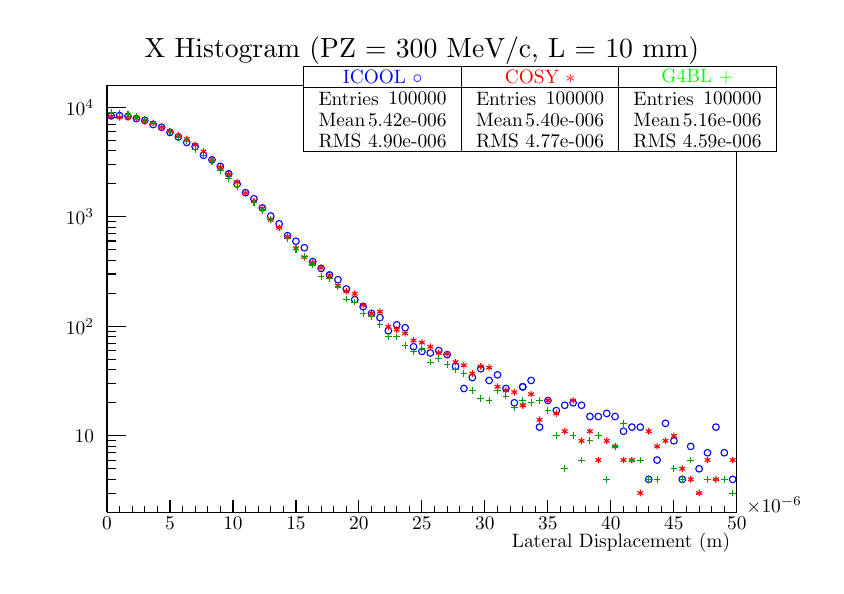
\begin{tikzpicture}
\definecolor{c}{rgb}{1,1,1};
\draw [color=c, fill=c] (0,0) rectangle (20,13.5632);
\draw [color=c, fill=c] (2,1.35632) rectangle (18,12.2069);
\definecolor{c}{rgb}{0,0,0};
\draw [c] (2,1.35632) -- (2,12.2069) -- (18,12.2069) -- (18,1.35632) -- (2,1.35632);
\definecolor{c}{rgb}{1,1,1};
\draw [color=c, fill=c] (2,1.35632) rectangle (18,12.2069);
\definecolor{c}{rgb}{0,0,0};
\draw [c] (2,1.35632) -- (2,12.2069) -- (18,12.2069) -- (18,1.35632) -- (2,1.35632);
\definecolor{c}{rgb}{0,0,1};
\foreach \P in
 {(2.10667,11.4283),(2.32,11.4346),(2.53333,11.415),(2.74667,11.3591),(2.96,11.3142),(3.17333,11.2073),(3.38667,11.1376),(3.6,11.0073),(3.81333,10.8909),(4.02667,10.7523),(4.24,10.6469),(4.45333,10.4248),(4.66667,10.3112),(4.88,10.1442),(5.09333,9.95
418),(5.30667,9.69383),(5.52,9.47692),(5.73333,9.32076),(5.94667,9.08827),(6.16,8.88275),(6.37333,8.6851),(6.58667,8.38382),(6.8,8.24262),(7.01333,8.07808),(7.22667,7.72502),(7.44,7.55162),(7.65333,7.38668),(7.86667,7.26574),(8.08,7.0308),(8.29333,6.
75977),(8.50667,6.58153),(8.72,6.40984),(8.93333,6.30386),(9.14667,5.96958),(9.36,6.11926),(9.57333,6.04674),(9.78667,5.56299),(10,5.44596),(10.2133,5.40429),(10.4267,5.46627),(10.64,5.36113),(10.8533,5.0637),(11.0667,4.50137),(11.28,4.77993),(11.493
3,5.00615),(11.7067,4.70667),(11.92,4.849),(12.1333,4.50137),(12.3467,4.13873),(12.56,4.54531)}{\draw[mark options={color=c,fill=c},mark size=2.402402pt,mark=o] plot coordinates {\P};}
\foreach \P in
 {(12.56,4.54531),(12.7733,4.70667),(12.9867,3.52145),(13.2,4.19768),(13.4133,3.94234),(13.6267,4.07674),(13.84,4.13873),(14.0533,4.07674),(14.2667,3.7911),(14.48,3.7911),(14.6933,3.86908),(14.9067,3.7911),(15.12,3.41631),(15.3333,3.52145),(15.5467,3
.52145),(15.76,2.19391),(15.9733,2.68387),(16.1867,3.61818),(16.4,3.17382),(16.6133,2.19391),(16.8267,3.0315),(17.04,2.46355),(17.2533,2.87014),(17.4667,3.52145),(17.68,2.87014),(17.8933,2.19391)}{\draw[mark options={color=c,fill=c},mark
 size=2.402402pt,mark=o] plot coordinates {\P};}
\definecolor{c}{rgb}{1,1,1};
\draw [color=c, fill=c] (7,10.5115) rectangle (11,12.6816);
\definecolor{c}{rgb}{0,0,0};
\draw [c] (7,10.5115) -- (11,10.5115);
\draw [c] (11,10.5115) -- (11,12.6816);
\draw [c] (11,12.6816) -- (7,12.6816);
\draw [c] (7,12.6816) -- (7,10.5115);
\draw[color=blue](9,12.4103) node[scale=0.7, rotate=0]{ICOOL $\circ$};
\draw [c] (7,12.1391) -- (11,12.1391);
\draw [anchor= west] (7.2,11.8678) node[scale=0.7, rotate=0]{Entries };
\draw [anchor= east] (10.8,11.8678) node[scale=0.7, rotate=0]{ 100000};
\draw [anchor= west] (7.2,11.3253) node[scale=0.7, rotate=0]{Mean  };
\draw [anchor= east] (10.8,11.3253) node[scale=0.7, rotate=0]{ 5.42e-006};
\draw [anchor= west] (7.2,10.7828) node[scale=0.7, rotate=0]{RMS   };
\draw [anchor= east] (10.8,10.7828) node[scale=0.7, rotate=0]{ 4.90e-006};
\draw [c] (2,1.35632) -- (18,1.35632);
\draw [anchor= east] (18,0.596782) node[scale=0.7, rotate=0]{Lateral Displacement (m)};
\draw [c] (2,1.68184) -- (2,1.35632);
\draw [c] (2.32,1.51908) -- (2.32,1.35632);
\draw [c] (2.64,1.51908) -- (2.64,1.35632);
\draw [c] (2.96,1.51908) -- (2.96,1.35632);
\draw [c] (3.28,1.51908) -- (3.28,1.35632);
\draw [c] (3.6,1.68184) -- (3.6,1.35632);
\draw [c] (3.92,1.51908) -- (3.92,1.35632);
\draw [c] (4.24,1.51908) -- (4.24,1.35632);
\draw [c] (4.56,1.51908) -- (4.56,1.35632);
\draw [c] (4.88,1.51908) -- (4.88,1.35632);
\draw [c] (5.2,1.68184) -- (5.2,1.35632);
\draw [c] (5.52,1.51908) -- (5.52,1.35632);
\draw [c] (5.84,1.51908) -- (5.84,1.35632);
\draw [c] (6.16,1.51908) -- (6.16,1.35632);
\draw [c] (6.48,1.51908) -- (6.48,1.35632);
\draw [c] (6.8,1.68184) -- (6.8,1.35632);
\draw [c] (7.12,1.51908) -- (7.12,1.35632);
\draw [c] (7.44,1.51908) -- (7.44,1.35632);
\draw [c] (7.76,1.51908) -- (7.76,1.35632);
\draw [c] (8.08,1.51908) -- (8.08,1.35632);
\draw [c] (8.4,1.68184) -- (8.4,1.35632);
\draw [c] (8.72,1.51908) -- (8.72,1.35632);
\draw [c] (9.04,1.51908) -- (9.04,1.35632);
\draw [c] (9.36,1.51908) -- (9.36,1.35632);
\draw [c] (9.68,1.51908) -- (9.68,1.35632);
\draw [c] (10,1.68184) -- (10,1.35632);
\draw [c] (10.32,1.51908) -- (10.32,1.35632);
\draw [c] (10.64,1.51908) -- (10.64,1.35632);
\draw [c] (10.96,1.51908) -- (10.96,1.35632);
\draw [c] (11.28,1.51908) -- (11.28,1.35632);
\draw [c] (11.6,1.68184) -- (11.6,1.35632);
\draw [c] (11.92,1.51908) -- (11.92,1.35632);
\draw [c] (12.24,1.51908) -- (12.24,1.35632);
\draw [c] (12.56,1.51908) -- (12.56,1.35632);
\draw [c] (12.88,1.51908) -- (12.88,1.35632);
\draw [c] (13.2,1.68184) -- (13.2,1.35632);
\draw [c] (13.52,1.51908) -- (13.52,1.35632);
\draw [c] (13.84,1.51908) -- (13.84,1.35632);
\draw [c] (14.16,1.51908) -- (14.16,1.35632);
\draw [c] (14.48,1.51908) -- (14.48,1.35632);
\draw [c] (14.8,1.68184) -- (14.8,1.35632);
\draw [c] (15.12,1.51908) -- (15.12,1.35632);
\draw [c] (15.44,1.51908) -- (15.44,1.35632);
\draw [c] (15.76,1.51908) -- (15.76,1.35632);
\draw [c] (16.08,1.51908) -- (16.08,1.35632);
\draw [c] (16.4,1.68184) -- (16.4,1.35632);
\draw [c] (16.72,1.51908) -- (16.72,1.35632);
\draw [c] (17.04,1.51908) -- (17.04,1.35632);
\draw [c] (17.36,1.51908) -- (17.36,1.35632);
\draw [c] (17.68,1.51908) -- (17.68,1.35632);
\draw [c] (18,1.68184) -- (18,1.35632);
\draw [c] (18,1.68184) -- (18,1.35632);
\draw [anchor=base] (2,0.908736) node[scale=0.7, rotate=0]{0};
\draw [anchor=base] (3.6,0.908736) node[scale=0.7, rotate=0]{5};
\draw [anchor=base] (5.2,0.908736) node[scale=0.7, rotate=0]{10};
\draw [anchor=base] (6.8,0.908736) node[scale=0.7, rotate=0]{15};
\draw [anchor=base] (8.4,0.908736) node[scale=0.7, rotate=0]{20};
\draw [anchor=base] (10,0.908736) node[scale=0.7, rotate=0]{25};
\draw [anchor=base] (11.6,0.908736) node[scale=0.7, rotate=0]{30};
\draw [anchor=base] (13.2,0.908736) node[scale=0.7, rotate=0]{35};
\draw [anchor=base] (14.8,0.908736) node[scale=0.7, rotate=0]{40};
\draw [anchor=base] (16.4,0.908736) node[scale=0.7, rotate=0]{45};
\draw [anchor=base] (18,0.908736) node[scale=0.7, rotate=0]{50};
\draw [anchor=base west] (18.07,1.35632) node[scale=0.7, rotate=0]{$\times10^{-6}$};
\draw [c] (2,1.35632) -- (2,12.2069);
\draw [c] (2.24,1.84628) -- (2,1.84628);
\draw [c] (2.24,2.19391) -- (2,2.19391);
\draw [c] (2.24,2.46355) -- (2,2.46355);
\draw [c] (2.24,2.68386) -- (2,2.68386);
\draw [c] (2.24,2.87014) -- (2,2.87014);
\draw [c] (2.24,3.03149) -- (2,3.03149);
\draw [c] (2.24,3.17382) -- (2,3.17382);
\draw [c] (2.48,3.30114) -- (2,3.30114);
\draw [anchor= east] (1.844,3.30114) node[scale=0.7, rotate=0]{10};
\draw [c] (2.24,4.13872) -- (2,4.13872);
\draw [c] (2.24,4.62868) -- (2,4.62868);
\draw [c] (2.24,4.97631) -- (2,4.97631);
\draw [c] (2.24,5.24595) -- (2,5.24595);
\draw [c] (2.24,5.46627) -- (2,5.46627);
\draw [c] (2.24,5.65254) -- (2,5.65254);
\draw [c] (2.24,5.8139) -- (2,5.8139);
\draw [c] (2.24,5.95623) -- (2,5.95623);
\draw [c] (2.48,6.08354) -- (2,6.08354);
\draw [anchor= east] (1.844,6.08354) node[scale=0.7, rotate=0]{$10^{2}$};
\draw [c] (2.24,6.92113) -- (2,6.92113);
\draw [c] (2.24,7.41109) -- (2,7.41109);
\draw [c] (2.24,7.75872) -- (2,7.75872);
\draw [c] (2.24,8.02836) -- (2,8.02836);
\draw [c] (2.24,8.24867) -- (2,8.24867);
\draw [c] (2.24,8.43495) -- (2,8.43495);
\draw [c] (2.24,8.5963) -- (2,8.5963);
\draw [c] (2.24,8.73863) -- (2,8.73863);
\draw [c] (2.48,8.86595) -- (2,8.86595);
\draw [anchor= east] (1.844,8.86595) node[scale=0.7, rotate=0]{$10^{3}$};
\draw [c] (2.24,9.70354) -- (2,9.70354);
\draw [c] (2.24,10.1935) -- (2,10.1935);
\draw [c] (2.24,10.5411) -- (2,10.5411);
\draw [c] (2.24,10.8108) -- (2,10.8108);
\draw [c] (2.24,11.0311) -- (2,11.0311);
\draw [c] (2.24,11.2174) -- (2,11.2174);
\draw [c] (2.24,11.3787) -- (2,11.3787);
\draw [c] (2.24,11.521) -- (2,11.521);
\draw [c] (2.48,11.6484) -- (2,11.6484);
\draw [anchor= east] (1.844,11.6484) node[scale=0.7, rotate=0]{$10^{4}$};
\definecolor{c}{rgb}{1,1,1};
\draw [color=c, fill=c] (7,10.5115) rectangle (11,12.6816);
\definecolor{c}{rgb}{0,0,0};
\draw [c] (7,10.5115) -- (11,10.5115);
\draw [c] (11,10.5115) -- (11,12.6816);
\draw [c] (11,12.6816) -- (7,12.6816);
\draw [c] (7,12.6816) -- (7,10.5115);
\draw[color=blue](9,12.4103) node[scale=0.7, rotate=0]{ICOOL $\circ$};
\draw [c] (7,12.1391) -- (11,12.1391);
\draw [anchor= west] (7.2,11.8678) node[scale=0.7, rotate=0]{Entries };
\draw [anchor= east] (10.8,11.8678) node[scale=0.7, rotate=0]{ 100000};
\draw [anchor= west] (7.2,11.3253) node[scale=0.7, rotate=0]{Mean  };
\draw [anchor= east] (10.8,11.3253) node[scale=0.7, rotate=0]{ 5.42e-006};
\draw [anchor= west] (7.2,10.7828) node[scale=0.7, rotate=0]{RMS   };
\draw [anchor= east] (10.8,10.7828) node[scale=0.7, rotate=0]{ 4.90e-006};
\draw (10,13.0816) node[scale=1, rotate=0]{X Histogram (PZ = 300 MeV/c, L = 10 mm)};
\definecolor{c}{rgb}{1,0,0};
\foreach \P in
 {(2.10667,11.4127),(2.32,11.3891),(2.53333,11.3888),(2.74667,11.3663),(2.96,11.2863),(3.17333,11.246),(3.38667,11.1372),(3.6,11.0335),(3.81333,10.9284),(4.02667,10.839),(4.24,10.6944),(4.45333,10.5241),(4.66667,10.3079),(4.88,10.1213),(5.09333,9.937
87),(5.30667,9.74744),(5.52,9.46667),(5.73333,9.25602),(5.94667,9.07208),(6.16,8.78603),(6.37333,8.58569),(6.58667,8.3565),(6.8,8.06408),(7.01333,7.83765),(7.22667,7.69991),(7.44,7.56942),(7.65333,7.37428),(7.86667,7.116),(8.08,6.96852),(8.29333,6.90
899),(8.50667,6.62089),(8.72,6.40984),(8.93333,6.4551),(9.14667,6.0714),(9.36,5.99585),(9.57333,5.90129),(9.78667,5.71969),(10,5.66968),(10.2133,5.56299),(10.4267,5.40429),(10.64,5.3829),(10.8533,5.17119),(11.0667,5.09149),(11.28,4.88211),(11.4933,5.
0637),(11.7067,5.03527),(11.92,4.54531),(12.1333,4.45576),(12.3467,4.40837),(12.56,4.07674)}{\draw[mark options={color=c,fill=c},mark size=2.402402pt,mark=asterisk] plot coordinates {\P};}
\foreach \P in
 {(12.56,4.07674),(12.7733,4.35904),(12.9867,3.70773),(13.2,4.19768),(13.4133,3.86908),(13.6267,3.41631),(13.84,4.19768),(14.0533,3.17382),(14.2667,3.41631),(14.48,2.68387),(14.6933,3.17382),(14.9067,3.0315),(15.12,2.68387),(15.3333,2.68387),(15.5467
,1.84628),(15.76,3.41631),(15.9733,3.0315),(16.1867,3.17382),(16.4,3.30114),(16.6133,2.46355),(16.8267,2.19391),(17.04,1.84628),(17.2533,2.68387),(17.4667,2.19391),(17.8933,2.68387)}{\draw[mark options={color=c,fill=c},mark
 size=2.402402pt,mark=asterisk] plot coordinates {\P};}
\definecolor{c}{rgb}{1,1,1};
\draw [color=c, fill=c] (11,10.5115) rectangle (15,12.6816);
\definecolor{c}{rgb}{0,0,0};
\draw [c] (11,10.5115) -- (15,10.5115);
\draw [c] (15,10.5115) -- (15,12.6816);
\draw [c] (15,12.6816) -- (11,12.6816);
\draw [c] (11,12.6816) -- (11,10.5115);
\draw [color=red](13,12.4103) node[scale=0.7, rotate=0]{COSY $*$};
\draw [c] (11,12.1391) -- (15,12.1391);
\draw [anchor= west] (11.2,11.8678) node[scale=0.7, rotate=0]{Entries };
\draw [anchor= east] (14.8,11.8678) node[scale=0.7, rotate=0]{ 100000};
\draw [anchor= west] (11.2,11.3253) node[scale=0.7, rotate=0]{Mean  };
\draw [anchor= east] (14.8,11.3253) node[scale=0.7, rotate=0]{ 5.40e-006};
\draw [anchor= west] (11.2,10.7828) node[scale=0.7, rotate=0]{RMS   };
\draw [anchor= east] (14.8,10.7828) node[scale=0.7, rotate=0]{ 4.77e-006};
\definecolor{c}{rgb}{1,1,1};
\draw [color=c, fill=c] (11,10.5115) rectangle (15,12.6816);
\definecolor{c}{rgb}{0,0,0};
\draw [c] (11,10.5115) -- (15,10.5115);
\draw [c] (15,10.5115) -- (15,12.6816);
\draw [c] (15,12.6816) -- (11,12.6816);
\draw [c] (11,12.6816) -- (11,10.5115);
\draw [color=red](13,12.4103) node[scale=0.7, rotate=0]{COSY $*$};
\draw [c] (11,12.1391) -- (15,12.1391);
\draw [anchor= west] (11.2,11.8678) node[scale=0.7, rotate=0]{Entries };
\draw [anchor= east] (14.8,11.8678) node[scale=0.7, rotate=0]{ 100000};
\draw [anchor= west] (11.2,11.3253) node[scale=0.7, rotate=0]{Mean  };
\draw [anchor= east] (14.8,11.3253) node[scale=0.7, rotate=0]{ 5.40e-006};
\draw [anchor= west] (11.2,10.7828) node[scale=0.7, rotate=0]{RMS   };
\draw [anchor= east] (14.8,10.7828) node[scale=0.7, rotate=0]{ 4.77e-006};
\definecolor{c}{rgb}{0,0.6,0};
\foreach \P in
 {(2.10667,11.513),(2.32,11.4834),(2.53333,11.4639),(2.74667,11.4062),(2.96,11.3302),(3.17333,11.2469),(3.38667,11.1404),(3.6,11.0315),(3.81333,10.8823),(4.02667,10.7873),(4.24,10.5671),(4.45333,10.4094),(4.66667,10.2666),(4.88,10.0436),(5.09333,9.84
317),(5.30667,9.63773),(5.52,9.45114),(5.73333,9.22948),(5.94667,9.01363),(6.16,8.79759),(6.37333,8.58111),(6.58667,8.31337),(6.8,8.04039),(7.01333,7.85451),(7.22667,7.6381),(7.44,7.35334),(7.65333,7.28824),(7.86667,7.07946),(8.08,6.77351),(8.29333,6
.69597),(8.50667,6.40058),(8.72,6.3337),(8.93333,6.13094),(9.14667,5.82891),(9.36,5.8139),(9.57333,5.59961),(9.78667,5.44596),(10,5.50589),(10.2133,5.17119),(10.4267,5.26989),(10.64,5.11864),(10.8533,4.97631),(11.0667,4.88211),(11.28,4.45576),(11.493
3,4.2539),(11.7067,4.19768),(11.92,4.45576),(12.1333,4.30761),(12.3467,4.01141),(12.56,4.19768)}{\draw[mark options={color=c,fill=c},mark size=2.402402pt,mark=+] plot coordinates {\P};}
\foreach \P in
 {(12.56,4.19768),(12.7733,4.13873),(12.9867,4.19768),(13.2,3.94234),(13.4133,3.30114),(13.6267,2.46355),(13.84,3.30114),(14.0533,2.68387),(14.2667,3.17382),(14.48,3.30114),(14.6933,2.19391),(14.9067,3.0315),(15.12,3.61818),(15.3333,2.68387),(15.5467
,2.68387),(15.76,2.19391),(15.9733,2.19391),(16.4,2.46355),(16.6133,2.19391),(16.8267,2.68387),(17.04,1.84628),(17.2533,2.19391),(17.4667,2.19391),(17.68,2.19391),(17.8933,1.84628)}{\draw[mark options={color=c,fill=c},mark size=2.402402pt,mark=+]
 plot coordinates {\P};}
\definecolor{c}{rgb}{1,1,1};
\draw [color=c, fill=c] (15,10.5115) rectangle (19,12.6816);
\definecolor{c}{rgb}{0,0,0};
\draw [c] (15,10.5115) -- (19,10.5115);
\draw [c] (19,10.5115) -- (19,12.6816);
\draw [c] (19,12.6816) -- (15,12.6816);
\draw [c] (15,12.6816) -- (15,10.5115);
\draw [color=green](17,12.4103) node[scale=0.7, rotate=0]{G4BL $+$};
\draw [c] (15,12.1391) -- (19,12.1391);
\draw [anchor= west] (15.2,11.8678) node[scale=0.7, rotate=0]{Entries };
\draw [anchor= east] (18.8,11.8678) node[scale=0.7, rotate=0]{ 100000};
\draw [anchor= west] (15.2,11.3253) node[scale=0.7, rotate=0]{Mean  };
\draw [anchor= east] (18.8,11.3253) node[scale=0.7, rotate=0]{ 5.16e-006};
\draw [anchor= west] (15.2,10.7828) node[scale=0.7, rotate=0]{RMS   };
\draw [anchor= east] (18.8,10.7828) node[scale=0.7, rotate=0]{ 4.59e-006};
\definecolor{c}{rgb}{1,1,1};
\draw [color=c, fill=c] (15,10.5115) rectangle (19,12.6816);
\definecolor{c}{rgb}{0,0,0};
\draw [c] (15,10.5115) -- (19,10.5115);
\draw [c] (19,10.5115) -- (19,12.6816);
\draw [c] (19,12.6816) -- (15,12.6816);
\draw [c] (15,12.6816) -- (15,10.5115);
\draw [color=green](17,12.4103) node[scale=0.7, rotate=0]{G4BL $+$};
\draw [c] (15,12.1391) -- (19,12.1391);
\draw [anchor= west] (15.2,11.8678) node[scale=0.7, rotate=0]{Entries };
\draw [anchor= east] (18.8,11.8678) node[scale=0.7, rotate=0]{ 100000};
\draw [anchor= west] (15.2,11.3253) node[scale=0.7, rotate=0]{Mean  };
\draw [anchor= east] (18.8,11.3253) node[scale=0.7, rotate=0]{ 5.16e-006};
\draw [anchor= west] (15.2,10.7828) node[scale=0.7, rotate=0]{RMS   };
\draw [anchor= east] (18.8,10.7828) node[scale=0.7, rotate=0]{ 4.59e-006};
\end{tikzpicture}
}\\
\frame{    \pgfdeclareplotmark{cross} {
\pgfpathmoveto{\pgfpoint{-0.3\pgfplotmarksize}{\pgfplotmarksize}}
\pgfpathlineto{\pgfpoint{+0.3\pgfplotmarksize}{\pgfplotmarksize}}
\pgfpathlineto{\pgfpoint{+0.3\pgfplotmarksize}{0.3\pgfplotmarksize}}
\pgfpathlineto{\pgfpoint{+1\pgfplotmarksize}{0.3\pgfplotmarksize}}
\pgfpathlineto{\pgfpoint{+1\pgfplotmarksize}{-0.3\pgfplotmarksize}}
\pgfpathlineto{\pgfpoint{+0.3\pgfplotmarksize}{-0.3\pgfplotmarksize}}
\pgfpathlineto{\pgfpoint{+0.3\pgfplotmarksize}{-1.\pgfplotmarksize}}
\pgfpathlineto{\pgfpoint{-0.3\pgfplotmarksize}{-1.\pgfplotmarksize}}
\pgfpathlineto{\pgfpoint{-0.3\pgfplotmarksize}{-0.3\pgfplotmarksize}}
\pgfpathlineto{\pgfpoint{-1.\pgfplotmarksize}{-0.3\pgfplotmarksize}}
\pgfpathlineto{\pgfpoint{-1.\pgfplotmarksize}{0.3\pgfplotmarksize}}
\pgfpathlineto{\pgfpoint{-0.3\pgfplotmarksize}{0.3\pgfplotmarksize}}
\pgfpathclose
\pgfusepathqstroke
}
\pgfdeclareplotmark{cross*} {
\pgfpathmoveto{\pgfpoint{-0.3\pgfplotmarksize}{\pgfplotmarksize}}
\pgfpathlineto{\pgfpoint{+0.3\pgfplotmarksize}{\pgfplotmarksize}}
\pgfpathlineto{\pgfpoint{+0.3\pgfplotmarksize}{0.3\pgfplotmarksize}}
\pgfpathlineto{\pgfpoint{+1\pgfplotmarksize}{0.3\pgfplotmarksize}}
\pgfpathlineto{\pgfpoint{+1\pgfplotmarksize}{-0.3\pgfplotmarksize}}
\pgfpathlineto{\pgfpoint{+0.3\pgfplotmarksize}{-0.3\pgfplotmarksize}}
\pgfpathlineto{\pgfpoint{+0.3\pgfplotmarksize}{-1.\pgfplotmarksize}}
\pgfpathlineto{\pgfpoint{-0.3\pgfplotmarksize}{-1.\pgfplotmarksize}}
\pgfpathlineto{\pgfpoint{-0.3\pgfplotmarksize}{-0.3\pgfplotmarksize}}
\pgfpathlineto{\pgfpoint{-1.\pgfplotmarksize}{-0.3\pgfplotmarksize}}
\pgfpathlineto{\pgfpoint{-1.\pgfplotmarksize}{0.3\pgfplotmarksize}}
\pgfpathlineto{\pgfpoint{-0.3\pgfplotmarksize}{0.3\pgfplotmarksize}}
\pgfpathclose
\pgfusepathqfillstroke
}
\pgfdeclareplotmark{newstar} {
\pgfpathmoveto{\pgfqpoint{0pt}{\pgfplotmarksize}}
\pgfpathlineto{\pgfqpointpolar{44}{0.5\pgfplotmarksize}}
\pgfpathlineto{\pgfqpointpolar{18}{\pgfplotmarksize}}
\pgfpathlineto{\pgfqpointpolar{-20}{0.5\pgfplotmarksize}}
\pgfpathlineto{\pgfqpointpolar{-54}{\pgfplotmarksize}}
\pgfpathlineto{\pgfqpointpolar{-90}{0.5\pgfplotmarksize}}
\pgfpathlineto{\pgfqpointpolar{234}{\pgfplotmarksize}}
\pgfpathlineto{\pgfqpointpolar{198}{0.5\pgfplotmarksize}}
\pgfpathlineto{\pgfqpointpolar{162}{\pgfplotmarksize}}
\pgfpathlineto{\pgfqpointpolar{134}{0.5\pgfplotmarksize}}
\pgfpathclose
\pgfusepathqstroke
}
\pgfdeclareplotmark{newstar*} {
\pgfpathmoveto{\pgfqpoint{0pt}{\pgfplotmarksize}}
\pgfpathlineto{\pgfqpointpolar{44}{0.5\pgfplotmarksize}}
\pgfpathlineto{\pgfqpointpolar{18}{\pgfplotmarksize}}
\pgfpathlineto{\pgfqpointpolar{-20}{0.5\pgfplotmarksize}}
\pgfpathlineto{\pgfqpointpolar{-54}{\pgfplotmarksize}}
\pgfpathlineto{\pgfqpointpolar{-90}{0.5\pgfplotmarksize}}
\pgfpathlineto{\pgfqpointpolar{234}{\pgfplotmarksize}}
\pgfpathlineto{\pgfqpointpolar{198}{0.5\pgfplotmarksize}}
\pgfpathlineto{\pgfqpointpolar{162}{\pgfplotmarksize}}
\pgfpathlineto{\pgfqpointpolar{134}{0.5\pgfplotmarksize}}
\pgfpathclose
\pgfusepathqfillstroke
}
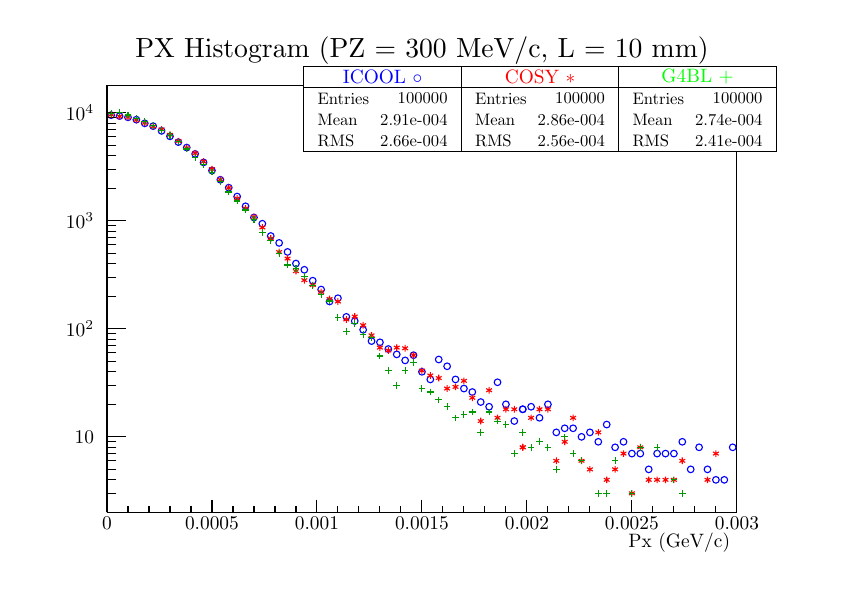
\begin{tikzpicture}
\definecolor{c}{rgb}{1,1,1};
\draw [color=c, fill=c] (0,0) rectangle (20,13.5632);
\draw [color=c, fill=c] (2,1.35632) rectangle (18,12.2069);
\definecolor{c}{rgb}{0,0,0};
\draw [c] (2,1.35632) -- (2,12.2069) -- (18,12.2069) -- (18,1.35632) -- (2,1.35632);
\definecolor{c}{rgb}{1,1,1};
\draw [color=c, fill=c] (2,1.35632) rectangle (18,12.2069);
\definecolor{c}{rgb}{0,0,0};
\draw [c] (2,1.35632) -- (2,12.2069) -- (18,12.2069) -- (18,1.35632) -- (2,1.35632);
\definecolor{c}{rgb}{0,0,1};
\foreach \P in
 {(2.10667,11.4453),(2.32,11.4218),(2.53333,11.3903),(2.74667,11.3309),(2.96,11.2373),(3.17333,11.1664),(3.38667,11.0453),(3.6,10.907),(3.81333,10.7611),(4.02667,10.6222),(4.24,10.4603),(4.45333,10.2437),(4.66667,10.0375),(4.88,9.80441),(5.09333,9.60
353),(5.30667,9.37823),(5.52,9.1303),(5.73333,8.84609),(5.94667,8.68713),(6.16,8.37561),(6.37333,8.20013),(6.58667,7.97135),(6.8,7.67615),(7.01333,7.51787),(7.22667,7.2409),(7.44,7.01592),(7.65333,6.712),(7.86667,6.79555),(8.08,6.32164),(8.29333,6.21
543),(8.50667,5.99412),(8.72,5.70673),(8.93333,5.67537),(9.14667,5.50484),(9.36,5.36905),(9.57333,5.21578),(9.78667,5.34833),(10,4.92627),(10.2133,4.7326),(10.4267,5.23892),(10.64,5.06663),(10.8533,4.7326),(11.0667,4.50123),(11.28,4.41291),(11.4933,4
.1584),(11.7067,4.03914),(11.92,4.66035),(12.1333,4.10026),(12.3467,3.67522),(12.56,3.9747)}{\draw[mark options={color=c,fill=c},mark size=2.402402pt,mark=o] plot coordinates {\P};}
\foreach \P in
 {(12.56,3.9747),(12.7733,4.03914),(12.9867,3.75744),(13.2,4.10026),(13.4133,3.38783),(13.6267,3.49152),(13.84,3.49152),(14.0533,3.27425),(14.2667,3.38783),(14.48,3.1487),(14.6933,3.58691),(14.9067,3.00834),(15.12,3.1487),(15.3333,2.84921),(15.5467,2
.84921),(15.76,2.44824),(15.9733,2.84921),(16.1867,2.84921),(16.4,2.84921),(16.6133,3.1487),(16.8267,2.44824),(17.04,3.00834),(17.2533,2.44824),(17.4667,2.18233),(17.68,2.18233),(17.8933,3.00834)}{\draw[mark options={color=c,fill=c},mark
 size=2.402402pt,mark=o] plot coordinates {\P};}
\definecolor{c}{rgb}{1,1,1};
\draw [color=c, fill=c] (7,10.5115) rectangle (11,12.6816);
\definecolor{c}{rgb}{0,0,0};
\draw [c] (7,10.5115) -- (11,10.5115);
\draw [c] (11,10.5115) -- (11,12.6816);
\draw [c] (11,12.6816) -- (7,12.6816);
\draw [c] (7,12.6816) -- (7,10.5115);
\draw[color=blue](9,12.4103) node[scale=0.7, rotate=0]{ICOOL $\circ$};
\draw [c] (7,12.1391) -- (11,12.1391);
\draw [anchor= west] (7.2,11.8678) node[scale=0.6, rotate=0]{Entries };
\draw [anchor= east] (10.8,11.8678) node[scale=0.6, rotate=0]{ 100000};
\draw [anchor= west] (7.2,11.3253) node[scale=0.6, rotate=0]{Mean  };
\draw [anchor= east] (10.8,11.3253) node[scale=0.6, rotate=0]{ 2.91e-004};
\draw [anchor= west] (7.2,10.7828) node[scale=0.6, rotate=0]{RMS   };
\draw [anchor= east] (10.8,10.7828) node[scale=0.6, rotate=0]{ 2.66e-004};
\draw [c] (2,1.35632) -- (18,1.35632);
\draw [anchor= east] (18,0.596782) node[scale=0.7, rotate=0]{Px (GeV/c)};
\draw [c] (2,1.68184) -- (2,1.35632);
\draw [c] (2.53333,1.51908) -- (2.53333,1.35632);
\draw [c] (3.06667,1.51908) -- (3.06667,1.35632);
\draw [c] (3.6,1.51908) -- (3.6,1.35632);
\draw [c] (4.13333,1.51908) -- (4.13333,1.35632);
\draw [c] (4.66667,1.68184) -- (4.66667,1.35632);
\draw [c] (5.2,1.51908) -- (5.2,1.35632);
\draw [c] (5.73333,1.51908) -- (5.73333,1.35632);
\draw [c] (6.26667,1.51908) -- (6.26667,1.35632);
\draw [c] (6.8,1.51908) -- (6.8,1.35632);
\draw [c] (7.33333,1.68184) -- (7.33333,1.35632);
\draw [c] (7.86667,1.51908) -- (7.86667,1.35632);
\draw [c] (8.4,1.51908) -- (8.4,1.35632);
\draw [c] (8.93333,1.51908) -- (8.93333,1.35632);
\draw [c] (9.46667,1.51908) -- (9.46667,1.35632);
\draw [c] (10,1.68184) -- (10,1.35632);
\draw [c] (10.5333,1.51908) -- (10.5333,1.35632);
\draw [c] (11.0667,1.51908) -- (11.0667,1.35632);
\draw [c] (11.6,1.51908) -- (11.6,1.35632);
\draw [c] (12.1333,1.51908) -- (12.1333,1.35632);
\draw [c] (12.6667,1.68184) -- (12.6667,1.35632);
\draw [c] (13.2,1.51908) -- (13.2,1.35632);
\draw [c] (13.7333,1.51908) -- (13.7333,1.35632);
\draw [c] (14.2667,1.51908) -- (14.2667,1.35632);
\draw [c] (14.8,1.51908) -- (14.8,1.35632);
\draw [c] (15.3333,1.68184) -- (15.3333,1.35632);
\draw [c] (15.8667,1.51908) -- (15.8667,1.35632);
\draw [c] (16.4,1.51908) -- (16.4,1.35632);
\draw [c] (16.9333,1.51908) -- (16.9333,1.35632);
\draw [c] (17.4667,1.51908) -- (17.4667,1.35632);
\draw [c] (18,1.68184) -- (18,1.35632);
\draw [c] (18,1.68184) -- (18,1.35632);
\draw [anchor=base] (2,0.908736) node[scale=0.7, rotate=0]{0};
\draw [anchor=base] (4.66667,0.908736) node[scale=0.7, rotate=0]{0.0005};
\draw [anchor=base] (7.33333,0.908736) node[scale=0.7, rotate=0]{0.001};
\draw [anchor=base] (10,0.908736) node[scale=0.7, rotate=0]{0.0015};
\draw [anchor=base] (12.6667,0.908736) node[scale=0.7, rotate=0]{0.002};
\draw [anchor=base] (15.3333,0.908736) node[scale=0.7, rotate=0]{0.0025};
\draw [anchor=base] (18,0.908736) node[scale=0.7, rotate=0]{0.003};
\draw [c] (2,1.35632) -- (2,12.2069);
\draw [c] (2.24,1.8395) -- (2,1.8395);
\draw [c] (2.24,2.18233) -- (2,2.18233);
\draw [c] (2.24,2.44824) -- (2,2.44824);
\draw [c] (2.24,2.66551) -- (2,2.66551);
\draw [c] (2.24,2.84921) -- (2,2.84921);
\draw [c] (2.24,3.00834) -- (2,3.00834);
\draw [c] (2.24,3.14869) -- (2,3.14869);
\draw [c] (2.48,3.27425) -- (2,3.27425);
\draw [anchor= east] (1.844,3.27425) node[scale=0.7, rotate=0]{10};
\draw [c] (2.24,4.10026) -- (2,4.10026);
\draw [c] (2.24,4.58344) -- (2,4.58344);
\draw [c] (2.24,4.92627) -- (2,4.92627);
\draw [c] (2.24,5.19218) -- (2,5.19218);
\draw [c] (2.24,5.40945) -- (2,5.40945);
\draw [c] (2.24,5.59315) -- (2,5.59315);
\draw [c] (2.24,5.75227) -- (2,5.75227);
\draw [c] (2.24,5.89263) -- (2,5.89263);
\draw [c] (2.48,6.01819) -- (2,6.01819);
\draw [anchor= east] (1.844,6.01819) node[scale=0.7, rotate=0]{$10^{2}$};
\draw [c] (2.24,6.8442) -- (2,6.8442);
\draw [c] (2.24,7.32738) -- (2,7.32738);
\draw [c] (2.24,7.67021) -- (2,7.67021);
\draw [c] (2.24,7.93612) -- (2,7.93612);
\draw [c] (2.24,8.15339) -- (2,8.15339);
\draw [c] (2.24,8.33709) -- (2,8.33709);
\draw [c] (2.24,8.49621) -- (2,8.49621);
\draw [c] (2.24,8.63657) -- (2,8.63657);
\draw [c] (2.48,8.76213) -- (2,8.76213);
\draw [anchor= east] (1.844,8.76213) node[scale=0.7, rotate=0]{$10^{3}$};
\draw [c] (2.24,9.58814) -- (2,9.58814);
\draw [c] (2.24,10.0713) -- (2,10.0713);
\draw [c] (2.24,10.4141) -- (2,10.4141);
\draw [c] (2.24,10.6801) -- (2,10.6801);
\draw [c] (2.24,10.8973) -- (2,10.8973);
\draw [c] (2.24,11.081) -- (2,11.081);
\draw [c] (2.24,11.2402) -- (2,11.2402);
\draw [c] (2.24,11.3805) -- (2,11.3805);
\draw [c] (2.48,11.5061) -- (2,11.5061);
\draw [anchor= east] (1.844,11.5061) node[scale=0.7, rotate=0]{$10^{4}$};
\definecolor{c}{rgb}{1,1,1};
\draw [color=c, fill=c] (7,10.5115) rectangle (11,12.6816);
\definecolor{c}{rgb}{0,0,0};
\draw [c] (7,10.5115) -- (11,10.5115);
\draw [c] (11,10.5115) -- (11,12.6816);
\draw [c] (11,12.6816) -- (7,12.6816);
\draw [c] (7,12.6816) -- (7,10.5115);
\draw[color=blue](9,12.4103) node[scale=0.7, rotate=0]{ICOOL $\circ$};
\draw [c] (7,12.1391) -- (11,12.1391);
\draw [anchor= west] (7.2,11.8678) node[scale=0.6, rotate=0]{Entries };
\draw [anchor= east] (10.8,11.8678) node[scale=0.6, rotate=0]{ 100000};
\draw [anchor= west] (7.2,11.3253) node[scale=0.6, rotate=0]{Mean  };
\draw [anchor= east] (10.8,11.3253) node[scale=0.6, rotate=0]{ 2.91e-004};
\draw [anchor= west] (7.2,10.7828) node[scale=0.6, rotate=0]{RMS   };
\draw [anchor= east] (10.8,10.7828) node[scale=0.6, rotate=0]{ 2.66e-004};
\draw (10,13.0816) node[scale=1, rotate=0]{PX Histogram (PZ = 300 MeV/c, L = 10 mm)};
\definecolor{c}{rgb}{1,0,0};
\foreach \P in
 {(2.10667,11.4572),(2.32,11.4157),(2.53333,11.3955),(2.74667,11.3215),(2.96,11.2483),(3.17333,11.1604),(3.38667,11.0843),(3.6,10.9456),(3.81333,10.7862),(4.02667,10.6109),(4.24,10.4785),(4.45333,10.2662),(4.66667,10.0745),(4.88,9.80838),(5.09333,9.5
9704),(5.30667,9.33039),(5.52,9.0757),(5.73333,8.85825),(5.94667,8.59206),(6.16,8.31127),(6.37333,7.96903),(6.58667,7.80259),(6.8,7.48353),(7.01333,7.25365),(7.22667,7.12903),(7.44,6.95235),(7.65333,6.77679),(7.86667,6.712),(8.08,6.25516),(8.29333,6.
33084),(8.50667,6.1099),(8.72,5.85224),(8.93333,5.54095),(9.14667,5.46759),(9.36,5.54095),(9.57333,5.52303),(9.78667,5.34833),(10,4.95569),(10.2133,4.83336),(10.4267,4.76714),(10.64,4.50123),(10.8533,4.54304),(11.0667,4.69702),(11.28,4.26681),(11.493
3,3.67522),(11.7067,4.45789),(11.92,3.75744),(12.1333,3.9747),(12.3467,3.9747),(12.56,3.00834)}{\draw[mark options={color=c,fill=c},mark size=2.402402pt,mark=asterisk] plot coordinates {\P};}
\foreach \P in
 {(12.56,3.00834),(12.7733,3.75744),(12.9867,3.9747),(13.2,3.9747),(13.4133,2.66551),(13.6267,3.1487),(13.84,3.75744),(14.0533,2.66551),(14.2667,2.44824),(14.48,3.38783),(14.6933,2.18233),(14.9067,2.44824),(15.12,2.84921),(15.3333,1.83951),(15.5467,3
.00834),(15.76,2.18233),(15.9733,2.18233),(16.1867,2.18233),(16.4,2.18233),(16.6133,2.66551),(17.2533,2.18233),(17.4667,2.84921)}{\draw[mark options={color=c,fill=c},mark size=2.402402pt,mark=asterisk] plot coordinates {\P};}
\definecolor{c}{rgb}{1,1,1};
\draw [color=c, fill=c] (11,10.5115) rectangle (15,12.6816);
\definecolor{c}{rgb}{0,0,0};
\draw [c] (11,10.5115) -- (15,10.5115);
\draw [c] (15,10.5115) -- (15,12.6816);
\draw [c] (15,12.6816) -- (11,12.6816);
\draw [c] (11,12.6816) -- (11,10.5115);
\draw [color=red](13,12.4103) node[scale=0.7, rotate=0]{COSY $*$};
\draw [c] (11,12.1391) -- (15,12.1391);
\draw [anchor= west] (11.2,11.8678) node[scale=0.6, rotate=0]{Entries };
\draw [anchor= east] (14.8,11.8678) node[scale=0.6, rotate=0]{ 100000};
\draw [anchor= west] (11.2,11.3253) node[scale=0.6, rotate=0]{Mean  };
\draw [anchor= east] (14.8,11.3253) node[scale=0.6, rotate=0]{ 2.86e-004};
\draw [anchor= west] (11.2,10.7828) node[scale=0.6, rotate=0]{RMS   };
\draw [anchor= east] (14.8,10.7828) node[scale=0.6, rotate=0]{ 2.56e-004};
\definecolor{c}{rgb}{1,1,1};
\draw [color=c, fill=c] (11,10.5115) rectangle (15,12.6816);
\definecolor{c}{rgb}{0,0,0};
\draw [c] (11,10.5115) -- (15,10.5115);
\draw [c] (15,10.5115) -- (15,12.6816);
\draw [c] (15,12.6816) -- (11,12.6816);
\draw [c] (11,12.6816) -- (11,10.5115);
\draw [color=red](13,12.4103) node[scale=0.7, rotate=0]{COSY $*$};
\draw [c] (11,12.1391) -- (15,12.1391);
\draw [anchor= west] (11.2,11.8678) node[scale=0.6, rotate=0]{Entries };
\draw [anchor= east] (14.8,11.8678) node[scale=0.6, rotate=0]{ 100000};
\draw [anchor= west] (11.2,11.3253) node[scale=0.6, rotate=0]{Mean  };
\draw [anchor= east] (14.8,11.3253) node[scale=0.6, rotate=0]{ 2.86e-004};
\draw [anchor= west] (11.2,10.7828) node[scale=0.6, rotate=0]{RMS   };
\draw [anchor= east] (14.8,10.7828) node[scale=0.6, rotate=0]{ 2.56e-004};
\definecolor{c}{rgb}{0,0.6,0};
\foreach \P in
 {(2.10667,11.4866),(2.32,11.5093),(2.53333,11.4504),(2.74667,11.3713),(2.96,11.2829),(3.17333,11.1867),(3.38667,11.0568),(3.6,10.9256),(3.81333,10.7654),(4.02667,10.5854),(4.24,10.3754),(4.45333,10.1878),(4.66667,9.99801),(4.88,9.76501),(5.09333,9.4
9265),(5.30667,9.26423),(5.52,9.03565),(5.73333,8.79388),(5.94667,8.46298),(6.16,8.26154),(6.37333,7.92895),(6.58667,7.64004),(6.8,7.54465),(7.01333,7.34317),(7.22667,7.11961),(7.44,6.89665),(7.65333,6.72524),(7.86667,6.31237),(8.08,5.95707),(8.29333
,6.15324),(8.50667,5.87932),(8.72,5.79615),(8.93333,5.32723),(9.14667,4.95569),(9.36,4.58344),(9.57333,4.95569),(9.78667,5.16811),(10,4.50123),(10.2133,4.41291),(10.4267,4.21384),(10.64,4.03914),(10.8533,3.75744),(11.0667,3.83435),(11.28,3.90659),(11
.4933,3.38783),(11.7067,3.90659),(11.92,3.67522),(12.1333,3.58691),(12.3467,2.84921),(12.56,3.38783)}{\draw[mark options={color=c,fill=c},mark size=2.402402pt,mark=+] plot coordinates {\P};}
\foreach \P in
 {(12.56,3.38783),(12.7733,3.00834),(12.9867,3.1487),(13.2,3.00834),(13.4133,2.44824),(13.6267,3.27425),(13.84,2.84921),(14.0533,2.66551),(14.48,1.83951),(14.6933,1.83951),(14.9067,2.66551),(15.3333,1.83951),(15.5467,3.00834),(15.9733,3.00834),(16.4,
2.18233),(16.6133,1.83951)}{\draw[mark options={color=c,fill=c},mark size=2.402402pt,mark=+] plot coordinates {\P};}
\definecolor{c}{rgb}{1,1,1};
\draw [color=c, fill=c] (15,10.5115) rectangle (19,12.6816);
\definecolor{c}{rgb}{0,0,0};
\draw [c] (15,10.5115) -- (19,10.5115);
\draw [c] (19,10.5115) -- (19,12.6816);
\draw [c] (19,12.6816) -- (15,12.6816);
\draw [c] (15,12.6816) -- (15,10.5115);
\draw [color=green](17,12.4103) node[scale=0.7, rotate=0]{G4BL $+$};
\draw [c] (15,12.1391) -- (19,12.1391);
\draw [anchor= west] (15.2,11.8678) node[scale=0.6, rotate=0]{Entries };
\draw [anchor= east] (18.8,11.8678) node[scale=0.6, rotate=0]{ 100000};
\draw [anchor= west] (15.2,11.3253) node[scale=0.6, rotate=0]{Mean  };
\draw [anchor= east] (18.8,11.3253) node[scale=0.6, rotate=0]{ 2.74e-004};
\draw [anchor= west] (15.2,10.7828) node[scale=0.6, rotate=0]{RMS   };
\draw [anchor= east] (18.8,10.7828) node[scale=0.6, rotate=0]{ 2.41e-004};
\definecolor{c}{rgb}{1,1,1};
\draw [color=c, fill=c] (15,10.5115) rectangle (19,12.6816);
\definecolor{c}{rgb}{0,0,0};
\draw [c] (15,10.5115) -- (19,10.5115);
\draw [c] (19,10.5115) -- (19,12.6816);
\draw [c] (19,12.6816) -- (15,12.6816);
\draw [c] (15,12.6816) -- (15,10.5115);
\draw [color=green](17,12.4103) node[scale=0.7, rotate=0]{G4BL $+$};
\draw [c] (15,12.1391) -- (19,12.1391);
\draw [anchor= west] (15.2,11.8678) node[scale=0.6, rotate=0]{Entries };
\draw [anchor= east] (18.8,11.8678) node[scale=0.6, rotate=0]{ 100000};
\draw [anchor= west] (15.2,11.3253) node[scale=0.6, rotate=0]{Mean  };
\draw [anchor= east] (18.8,11.3253) node[scale=0.6, rotate=0]{ 2.74e-004};
\draw [anchor= west] (15.2,10.7828) node[scale=0.6, rotate=0]{RMS   };
\draw [anchor= east] (18.8,10.7828) node[scale=0.6, rotate=0]{ 2.41e-004};
\end{tikzpicture}
}\\
\frame{\pgfdeclareplotmark{cross} {
\pgfpathmoveto{\pgfpoint{-0.3\pgfplotmarksize}{\pgfplotmarksize}}
\pgfpathlineto{\pgfpoint{+0.3\pgfplotmarksize}{\pgfplotmarksize}}
\pgfpathlineto{\pgfpoint{+0.3\pgfplotmarksize}{0.3\pgfplotmarksize}}
\pgfpathlineto{\pgfpoint{+1\pgfplotmarksize}{0.3\pgfplotmarksize}}
\pgfpathlineto{\pgfpoint{+1\pgfplotmarksize}{-0.3\pgfplotmarksize}}
\pgfpathlineto{\pgfpoint{+0.3\pgfplotmarksize}{-0.3\pgfplotmarksize}}
\pgfpathlineto{\pgfpoint{+0.3\pgfplotmarksize}{-1.\pgfplotmarksize}}
\pgfpathlineto{\pgfpoint{-0.3\pgfplotmarksize}{-1.\pgfplotmarksize}}
\pgfpathlineto{\pgfpoint{-0.3\pgfplotmarksize}{-0.3\pgfplotmarksize}}
\pgfpathlineto{\pgfpoint{-1.\pgfplotmarksize}{-0.3\pgfplotmarksize}}
\pgfpathlineto{\pgfpoint{-1.\pgfplotmarksize}{0.3\pgfplotmarksize}}
\pgfpathlineto{\pgfpoint{-0.3\pgfplotmarksize}{0.3\pgfplotmarksize}}
\pgfpathclose
\pgfusepathqstroke
}
\pgfdeclareplotmark{cross*} {
\pgfpathmoveto{\pgfpoint{-0.3\pgfplotmarksize}{\pgfplotmarksize}}
\pgfpathlineto{\pgfpoint{+0.3\pgfplotmarksize}{\pgfplotmarksize}}
\pgfpathlineto{\pgfpoint{+0.3\pgfplotmarksize}{0.3\pgfplotmarksize}}
\pgfpathlineto{\pgfpoint{+1\pgfplotmarksize}{0.3\pgfplotmarksize}}
\pgfpathlineto{\pgfpoint{+1\pgfplotmarksize}{-0.3\pgfplotmarksize}}
\pgfpathlineto{\pgfpoint{+0.3\pgfplotmarksize}{-0.3\pgfplotmarksize}}
\pgfpathlineto{\pgfpoint{+0.3\pgfplotmarksize}{-1.\pgfplotmarksize}}
\pgfpathlineto{\pgfpoint{-0.3\pgfplotmarksize}{-1.\pgfplotmarksize}}
\pgfpathlineto{\pgfpoint{-0.3\pgfplotmarksize}{-0.3\pgfplotmarksize}}
\pgfpathlineto{\pgfpoint{-1.\pgfplotmarksize}{-0.3\pgfplotmarksize}}
\pgfpathlineto{\pgfpoint{-1.\pgfplotmarksize}{0.3\pgfplotmarksize}}
\pgfpathlineto{\pgfpoint{-0.3\pgfplotmarksize}{0.3\pgfplotmarksize}}
\pgfpathclose
\pgfusepathqfillstroke
}
\pgfdeclareplotmark{newstar} {
\pgfpathmoveto{\pgfqpoint{0pt}{\pgfplotmarksize}}
\pgfpathlineto{\pgfqpointpolar{44}{0.5\pgfplotmarksize}}
\pgfpathlineto{\pgfqpointpolar{18}{\pgfplotmarksize}}
\pgfpathlineto{\pgfqpointpolar{-20}{0.5\pgfplotmarksize}}
\pgfpathlineto{\pgfqpointpolar{-54}{\pgfplotmarksize}}
\pgfpathlineto{\pgfqpointpolar{-90}{0.5\pgfplotmarksize}}
\pgfpathlineto{\pgfqpointpolar{234}{\pgfplotmarksize}}
\pgfpathlineto{\pgfqpointpolar{198}{0.5\pgfplotmarksize}}
\pgfpathlineto{\pgfqpointpolar{162}{\pgfplotmarksize}}
\pgfpathlineto{\pgfqpointpolar{134}{0.5\pgfplotmarksize}}
\pgfpathclose
\pgfusepathqstroke
}
\pgfdeclareplotmark{newstar*} {
\pgfpathmoveto{\pgfqpoint{0pt}{\pgfplotmarksize}}
\pgfpathlineto{\pgfqpointpolar{44}{0.5\pgfplotmarksize}}
\pgfpathlineto{\pgfqpointpolar{18}{\pgfplotmarksize}}
\pgfpathlineto{\pgfqpointpolar{-20}{0.5\pgfplotmarksize}}
\pgfpathlineto{\pgfqpointpolar{-54}{\pgfplotmarksize}}
\pgfpathlineto{\pgfqpointpolar{-90}{0.5\pgfplotmarksize}}
\pgfpathlineto{\pgfqpointpolar{234}{\pgfplotmarksize}}
\pgfpathlineto{\pgfqpointpolar{198}{0.5\pgfplotmarksize}}
\pgfpathlineto{\pgfqpointpolar{162}{\pgfplotmarksize}}
\pgfpathlineto{\pgfqpointpolar{134}{0.5\pgfplotmarksize}}
\pgfpathclose
\pgfusepathqfillstroke
}
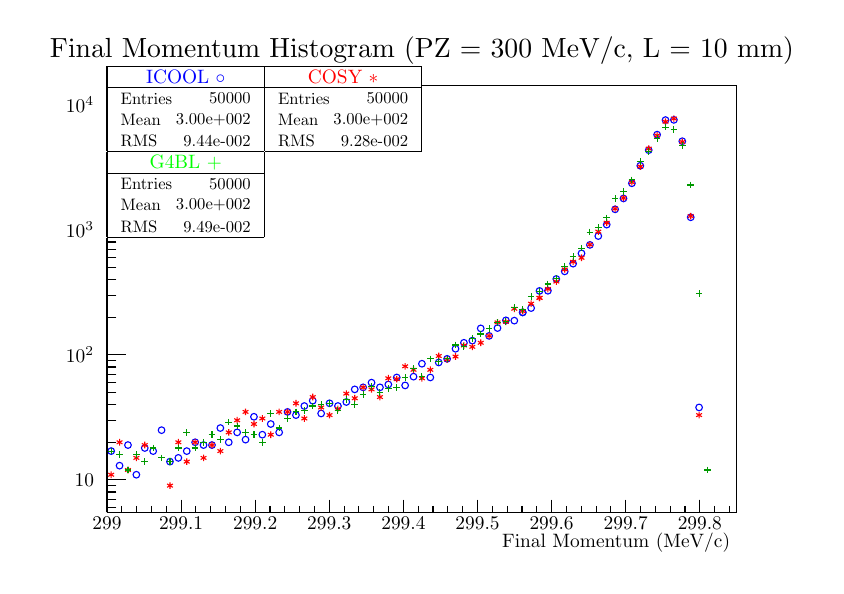
\begin{tikzpicture}
\definecolor{c}{rgb}{1,1,1};
\draw [color=c, fill=c] (0,0) rectangle (20,13.5632);
\draw [color=c, fill=c] (2,1.35632) rectangle (18,12.2069);
\definecolor{c}{rgb}{0,0,0};
\draw [c] (2,1.35632) -- (2,12.2069) -- (18,12.2069) -- (18,1.35632) -- (2,1.35632);
\definecolor{c}{rgb}{1,1,1};
\draw [color=c, fill=c] (2,1.35632) rectangle (18,12.2069);
\definecolor{c}{rgb}{0,0,0};
\draw [c] (2,1.35632) -- (2,12.2069) -- (18,12.2069) -- (18,1.35632) -- (2,1.35632);
\definecolor{c}{rgb}{0,0,1};
\foreach \P in
 {(2.10667,2.9123),(2.32,2.54241),(2.53333,3.06567),(2.74667,2.31207),(2.96,2.99111),(3.17333,2.9123),(3.38667,3.44407),(3.6,2.64459),(3.81333,2.73972),(4.02667,2.9123),(4.24,3.13639),(4.45333,3.06567),(4.66667,3.06567),(4.88,3.49815),(5.09333,3.1363
9),(5.30667,3.38778),(5.52,3.20366),(5.73333,3.78445),(5.94667,3.3291),(6.16,3.60033),(6.37333,3.38778),(6.58667,3.90801),(6.8,3.82688),(7.01333,4.05722),(7.22667,4.19185),(7.44,3.86805),(7.65333,4.12618),(7.86667,4.05722),(8.08,4.15941),(8.29333,4.4
8016),(8.50667,4.53123),(8.72,4.65121),(8.93333,4.53123),(9.14667,4.60446),(9.36,4.78263),(9.57333,4.58048),(9.78667,4.80336),(10,5.13147),(10.2133,4.78263),(10.4267,5.16354),(10.64,5.25549),(10.8533,5.51182),(11.0667,5.66324),(11.28,5.71732),(11.493
3,6.02923),(11.7067,5.83906),(11.92,6.03767),(12.1333,6.2333),(12.3467,6.22599),(12.56,6.43644)}{\draw[mark options={color=c,fill=c},mark size=2.402402pt,mark=o] plot coordinates {\P};}
\foreach \P in
 {(12.56,6.43644),(12.7733,6.54535),(12.9867,6.98074),(13.2,6.98498),(13.4133,7.28417),(13.6267,7.47762),(13.84,7.67316),(14.0533,7.93436),(14.2667,8.15025),(14.48,8.37443),(14.6933,8.66439),(14.9067,9.05322),(15.12,9.3294),(15.3333,9.71502),(15.5467
,10.1603),(15.76,10.5563),(15.9733,10.9505),(16.1867,11.3204),(16.4,11.3257),(16.6133,10.7834),(16.8267,8.85132),(17.04,4.02141)}{\draw[mark options={color=c,fill=c},mark size=2.402402pt,mark=o] plot coordinates {\P};}
\definecolor{c}{rgb}{1,1,1};
\draw [color=c, fill=c] (2,10.5115) rectangle (6,12.6816);
\definecolor{c}{rgb}{0,0,0};
\draw [c] (2,10.5115) -- (6,10.5115);
\draw [c] (6,10.5115) -- (6,12.6816);
\draw [c] (6,12.6816) -- (2,12.6816);
\draw [c] (2,12.6816) -- (2,10.5115);
\draw[color=blue](4,12.4103) node[scale=0.7, rotate=0]{ICOOL $\circ$};
\draw [c] (2,12.1391) -- (6,12.1391);
\draw [anchor= west] (2.2,11.8678) node[scale=0.6, rotate=0]{Entries };
\draw [anchor= east] (5.8,11.8678) node[scale=0.6, rotate=0]{ 50000};
\draw [anchor= west] (2.2,11.3253) node[scale=0.6, rotate=0]{Mean  };
\draw [anchor= east] (5.8,11.3253) node[scale=0.6, rotate=0]{ 3.00e+002};
\draw [anchor= west] (2.2,10.7828) node[scale=0.6, rotate=0]{RMS   };
\draw [anchor= east] (5.8,10.7828) node[scale=0.6, rotate=0]{ 9.44e-002};
\draw [c] (2,1.35632) -- (18,1.35632);
\draw [anchor= east] (18,0.596782) node[scale=0.7, rotate=0]{Final Momentum (MeV/c)};
\draw [c] (2,1.68184) -- (2,1.35632);
\draw [c] (2.37647,1.51908) -- (2.37647,1.35632);
\draw [c] (2.75294,1.51908) -- (2.75294,1.35632);
\draw [c] (3.12941,1.51908) -- (3.12941,1.35632);
\draw [c] (3.50588,1.51908) -- (3.50588,1.35632);
\draw [c] (3.88235,1.68184) -- (3.88235,1.35632);
\draw [c] (4.25882,1.51908) -- (4.25882,1.35632);
\draw [c] (4.63529,1.51908) -- (4.63529,1.35632);
\draw [c] (5.01176,1.51908) -- (5.01176,1.35632);
\draw [c] (5.38824,1.51908) -- (5.38824,1.35632);
\draw [c] (5.76471,1.68184) -- (5.76471,1.35632);
\draw [c] (6.14118,1.51908) -- (6.14118,1.35632);
\draw [c] (6.51765,1.51908) -- (6.51765,1.35632);
\draw [c] (6.89412,1.51908) -- (6.89412,1.35632);
\draw [c] (7.27059,1.51908) -- (7.27059,1.35632);
\draw [c] (7.64706,1.68184) -- (7.64706,1.35632);
\draw [c] (8.02353,1.51908) -- (8.02353,1.35632);
\draw [c] (8.4,1.51908) -- (8.4,1.35632);
\draw [c] (8.77647,1.51908) -- (8.77647,1.35632);
\draw [c] (9.15294,1.51908) -- (9.15294,1.35632);
\draw [c] (9.52941,1.68184) -- (9.52941,1.35632);
\draw [c] (9.90588,1.51908) -- (9.90588,1.35632);
\draw [c] (10.2824,1.51908) -- (10.2824,1.35632);
\draw [c] (10.6588,1.51908) -- (10.6588,1.35632);
\draw [c] (11.0353,1.51908) -- (11.0353,1.35632);
\draw [c] (11.4118,1.68184) -- (11.4118,1.35632);
\draw [c] (11.7882,1.51908) -- (11.7882,1.35632);
\draw [c] (12.1647,1.51908) -- (12.1647,1.35632);
\draw [c] (12.5412,1.51908) -- (12.5412,1.35632);
\draw [c] (12.9176,1.51908) -- (12.9176,1.35632);
\draw [c] (13.2941,1.68184) -- (13.2941,1.35632);
\draw [c] (13.6706,1.51908) -- (13.6706,1.35632);
\draw [c] (14.0471,1.51908) -- (14.0471,1.35632);
\draw [c] (14.4235,1.51908) -- (14.4235,1.35632);
\draw [c] (14.8,1.51908) -- (14.8,1.35632);
\draw [c] (15.1765,1.68184) -- (15.1765,1.35632);
\draw [c] (15.5529,1.51908) -- (15.5529,1.35632);
\draw [c] (15.9294,1.51908) -- (15.9294,1.35632);
\draw [c] (16.3059,1.51908) -- (16.3059,1.35632);
\draw [c] (16.6824,1.51908) -- (16.6824,1.35632);
\draw [c] (17.0588,1.68184) -- (17.0588,1.35632);
\draw [c] (17.0588,1.68184) -- (17.0588,1.35632);
\draw [c] (17.4353,1.51908) -- (17.4353,1.35632);
\draw [c] (17.8118,1.51908) -- (17.8118,1.35632);
\draw [anchor=base] (2,0.908736) node[scale=0.7, rotate=0]{299};
\draw [anchor=base] (3.88235,0.908736) node[scale=0.7, rotate=0]{299.1};
\draw [anchor=base] (5.76471,0.908736) node[scale=0.7, rotate=0]{299.2};
\draw [anchor=base] (7.64706,0.908736) node[scale=0.7, rotate=0]{299.3};
\draw [anchor=base] (9.52941,0.908736) node[scale=0.7, rotate=0]{299.4};
\draw [anchor=base] (11.4118,0.908736) node[scale=0.7, rotate=0]{299.5};
\draw [anchor=base] (13.2941,0.908736) node[scale=0.7, rotate=0]{299.6};
\draw [anchor=base] (15.1765,0.908736) node[scale=0.7, rotate=0]{299.7};
\draw [anchor=base] (17.0588,0.908736) node[scale=0.7, rotate=0]{299.8};
\draw [c] (2,1.35632) -- (2,12.2069);
\draw [c] (2.24,1.47629) -- (2,1.47629);
\draw [c] (2.24,1.68884) -- (2,1.68884);
\draw [c] (2.24,1.87296) -- (2,1.87296);
\draw [c] (2.24,2.03537) -- (2,2.03537);
\draw [c] (2.48,2.18064) -- (2,2.18064);
\draw [anchor= east] (1.844,2.18064) node[scale=0.7, rotate=0]{10};
\draw [c] (2.24,3.13639) -- (2,3.13639);
\draw [c] (2.24,3.69546) -- (2,3.69546);
\draw [c] (2.24,4.09213) -- (2,4.09213);
\draw [c] (2.24,4.39981) -- (2,4.39981);
\draw [c] (2.24,4.65121) -- (2,4.65121);
\draw [c] (2.24,4.86376) -- (2,4.86376);
\draw [c] (2.24,5.04788) -- (2,5.04788);
\draw [c] (2.24,5.21028) -- (2,5.21028);
\draw [c] (2.48,5.35556) -- (2,5.35556);
\draw [anchor= east] (1.844,5.35556) node[scale=0.7, rotate=0]{$10^{2}$};
\draw [c] (2.24,6.3113) -- (2,6.3113);
\draw [c] (2.24,6.87037) -- (2,6.87037);
\draw [c] (2.24,7.26704) -- (2,7.26704);
\draw [c] (2.24,7.57472) -- (2,7.57472);
\draw [c] (2.24,7.82612) -- (2,7.82612);
\draw [c] (2.24,8.03867) -- (2,8.03867);
\draw [c] (2.24,8.22279) -- (2,8.22279);
\draw [c] (2.24,8.38519) -- (2,8.38519);
\draw [c] (2.48,8.53047) -- (2,8.53047);
\draw [anchor= east] (1.844,8.53047) node[scale=0.7, rotate=0]{$10^{3}$};
\draw [c] (2.24,9.48621) -- (2,9.48621);
\draw [c] (2.24,10.0453) -- (2,10.0453);
\draw [c] (2.24,10.442) -- (2,10.442);
\draw [c] (2.24,10.7496) -- (2,10.7496);
\draw [c] (2.24,11.001) -- (2,11.001);
\draw [c] (2.24,11.2136) -- (2,11.2136);
\draw [c] (2.24,11.3977) -- (2,11.3977);
\draw [c] (2.24,11.5601) -- (2,11.5601);
\draw [c] (2.48,11.7054) -- (2,11.7054);
\draw [anchor= east] (1.844,11.7054) node[scale=0.7, rotate=0]{$10^{4}$};
\definecolor{c}{rgb}{1,1,1};
\draw [color=c, fill=c] (2,10.5115) rectangle (6,12.6816);
\definecolor{c}{rgb}{0,0,0};
\draw [c] (2,10.5115) -- (6,10.5115);
\draw [c] (6,10.5115) -- (6,12.6816);
\draw [c] (6,12.6816) -- (2,12.6816);
\draw [c] (2,12.6816) -- (2,10.5115);
\draw[color=blue](4,12.4103) node[scale=0.7, rotate=0]{ICOOL $\circ$};
\draw [c] (2,12.1391) -- (6,12.1391);
\draw [anchor= west] (2.2,11.8678) node[scale=0.6, rotate=0]{Entries };
\draw [anchor= east] (5.8,11.8678) node[scale=0.6, rotate=0]{ 50000};
\draw [anchor= west] (2.2,11.3253) node[scale=0.6, rotate=0]{Mean  };
\draw [anchor= east] (5.8,11.3253) node[scale=0.6, rotate=0]{ 3.00e+002};
\draw [anchor= west] (2.2,10.7828) node[scale=0.6, rotate=0]{RMS   };
\draw [anchor= east] (5.8,10.7828) node[scale=0.6, rotate=0]{ 9.44e-002};
\draw (10,13.0816) node[scale=1, rotate=0]{Final Momentum Histogram (PZ = 300 MeV/c, L = 10 mm)};
\definecolor{c}{rgb}{1,0,0};
\foreach \P in
 {(2.10667,2.31207),(2.32,3.13639),(2.53333,2.43204),(2.74667,2.73972),(2.96,3.06567),(3.6,2.03537),(3.81333,3.13639),(4.02667,2.64459),(4.24,3.13639),(4.45333,2.73972),(4.66667,3.06567),(4.88,2.9123),(5.09333,3.38778),(5.30667,3.69546),(5.52,3.90801
),(5.73333,3.60033),(5.94667,3.74068),(6.16,3.3291),(6.37333,3.90801),(6.58667,3.90801),(6.8,4.12618),(7.01333,3.74068),(7.22667,4.28484),(7.44,4.02141),(7.65333,3.82688),(7.86667,3.98464),(8.08,4.37196),(8.29333,4.25454),(8.50667,4.53123),(8.72,4.48
016),(8.93333,4.28484),(9.14667,4.76157),(9.36,4.7402),(9.57333,5.06501),(9.78667,4.97715),(10,4.76157),(10.2133,4.97715),(10.4267,5.3277),(10.64,5.24059),(10.8533,5.31356),(11.0667,5.59541),(11.28,5.56021),(11.4933,5.66324),(11.7067,5.83906),(11.92,
6.18126),(12.1333,6.19633),(12.3467,6.52779),(12.56,6.46756),(12.7733,6.65706),(12.9867,6.80448)}{\draw[mark options={color=c,fill=c},mark size=2.402402pt,mark=asterisk] plot coordinates {\P};}
\foreach \P in
 {(12.9867,6.80448),(13.2,7.03074),(13.4133,7.21792),(13.6267,7.52703),(13.84,7.7211),(14.0533,7.82152),(14.2667,8.15569),(14.48,8.48705),(14.6933,8.71355),(14.9067,9.06824),(15.12,9.34247),(15.3333,9.73933),(15.5467,10.142),(15.76,10.5961),(15.9733,
10.9308),(16.1867,11.2777),(16.4,11.3569),(16.6133,10.7644),(16.8267,8.88158),(17.04,3.82688)}{\draw[mark options={color=c,fill=c},mark size=2.402402pt,mark=asterisk] plot coordinates {\P};}
\definecolor{c}{rgb}{1,1,1};
\draw [color=c, fill=c] (6,10.5115) rectangle (10,12.6816);
\definecolor{c}{rgb}{0,0,0};
\draw [c] (6,10.5115) -- (10,10.5115);
\draw [c] (10,10.5115) -- (10,12.6816);
\draw [c] (10,12.6816) -- (6,12.6816);
\draw [c] (6,12.6816) -- (6,10.5115);
\draw [color=red](8,12.4103) node[scale=0.7, rotate=0]{COSY $*$};
\draw [c] (6,12.1391) -- (10,12.1391);
\draw [anchor= west] (6.2,11.8678) node[scale=0.6, rotate=0]{Entries };
\draw [anchor= east] (9.8,11.8678) node[scale=0.6, rotate=0]{ 50000};
\draw [anchor= west] (6.2,11.3253) node[scale=0.6, rotate=0]{Mean  };
\draw [anchor= east] (9.8,11.3253) node[scale=0.6, rotate=0]{ 3.00e+002};
\draw [anchor= west] (6.2,10.7828) node[scale=0.6, rotate=0]{RMS   };
\draw [anchor= east] (9.8,10.7828) node[scale=0.6, rotate=0]{ 9.28e-002};
\definecolor{c}{rgb}{1,1,1};
\draw [color=c, fill=c] (6,10.5115) rectangle (10,12.6816);
\definecolor{c}{rgb}{0,0,0};
\draw [c] (6,10.5115) -- (10,10.5115);
\draw [c] (10,10.5115) -- (10,12.6816);
\draw [c] (10,12.6816) -- (6,12.6816);
\draw [c] (6,12.6816) -- (6,10.5115);
\draw [color=red](8,12.4103) node[scale=0.7, rotate=0]{COSY $*$};
\draw [c] (6,12.1391) -- (10,12.1391);
\draw [anchor= west] (6.2,11.8678) node[scale=0.6, rotate=0]{Entries };
\draw [anchor= east] (9.8,11.8678) node[scale=0.6, rotate=0]{ 50000};
\draw [anchor= west] (6.2,11.3253) node[scale=0.6, rotate=0]{Mean  };
\draw [anchor= east] (9.8,11.3253) node[scale=0.6, rotate=0]{ 3.00e+002};
\draw [anchor= west] (6.2,10.7828) node[scale=0.6, rotate=0]{RMS   };
\draw [anchor= east] (9.8,10.7828) node[scale=0.6, rotate=0]{ 9.28e-002};
\definecolor{c}{rgb}{0,0.6,0};
\foreach \P in
 {(2.10667,2.9123),(2.32,2.82871),(2.53333,2.43204),(2.74667,2.82871),(2.96,2.64459),(3.17333,2.99111),(3.38667,2.73972),(3.6,2.64459),(3.81333,2.99111),(4.02667,3.38778),(4.24,2.99111),(4.45333,3.13639),(4.66667,3.3291),(4.88,3.20366),(5.09333,3.648
72),(5.30667,3.55019),(5.52,3.38778),(5.73333,3.3291),(5.94667,3.13639),(6.16,3.86805),(6.37333,3.49815),(6.58667,3.74068),(6.8,3.90801),(7.01333,3.94686),(7.22667,4.05722),(7.44,4.09213),(7.65333,4.12618),(7.86667,3.94686),(8.08,4.22355),(8.29333,4.
09213),(8.50667,4.34353),(8.72,4.55608),(8.93333,4.39981),(9.14667,4.50593),(9.36,4.53123),(9.57333,4.78263),(9.78667,5.01297),(10,4.80336),(10.2133,5.25549),(10.4267,5.19488),(10.64,5.25549),(10.8533,5.60695),(11.0667,5.57204),(11.28,5.76936),(11.49
33,5.88678),(11.7067,6.02075),(11.92,6.17366),(12.1333,6.21124),(12.3467,6.55694),(12.56,6.50401)}{\draw[mark options={color=c,fill=c},mark size=2.402402pt,mark=+] plot coordinates {\P};}
\foreach \P in
 {(12.56,6.50401),(12.7733,6.83311),(12.9867,6.96367),(13.2,7.15582),(13.4133,7.30445),(13.6267,7.5939),(13.84,7.84891),(14.0533,8.0679),(14.2667,8.47562),(14.48,8.58455),(14.6933,8.83705),(14.9067,9.32243),(15.12,9.51081),(15.3333,9.80159),(15.5467,
10.2708),(15.76,10.5268),(15.9733,10.8514),(16.1867,11.1414),(16.4,11.0812),(16.6133,10.6711),(16.8267,9.6699),(17.04,6.91559),(17.2533,2.43204)}{\draw[mark options={color=c,fill=c},mark size=2.402402pt,mark=+] plot coordinates {\P};}
\definecolor{c}{rgb}{1,1,1};
\draw [color=c, fill=c] (2,8.34138) rectangle (6,10.5115);
\definecolor{c}{rgb}{0,0,0};
\draw [c] (2,8.34138) -- (6,8.34138);
\draw [c] (6,8.34138) -- (6,10.5115);
\draw [c] (6,10.5115) -- (2,10.5115);
\draw [c] (2,10.5115) -- (2,8.34138);
\draw [color=green](4,10.2402) node[scale=0.7, rotate=0]{G4BL $+$};
\draw [c] (2,9.96897) -- (6,9.96897);
\draw [anchor= west] (2.2,9.6977) node[scale=0.6, rotate=0]{Entries };
\draw [anchor= east] (5.8,9.6977) node[scale=0.6, rotate=0]{ 50000};
\draw [anchor= west] (2.2,9.15517) node[scale=0.6, rotate=0]{Mean  };
\draw [anchor= east] (5.8,9.15517) node[scale=0.6, rotate=0]{ 3.00e+002};
\draw [anchor= west] (2.2,8.61264) node[scale=0.6, rotate=0]{RMS   };
\draw [anchor= east] (5.8,8.61264) node[scale=0.6, rotate=0]{ 9.49e-002};
\definecolor{c}{rgb}{1,1,1};
\draw [color=c, fill=c] (2,8.34138) rectangle (6,10.5115);
\definecolor{c}{rgb}{0,0,0};
\draw [c] (2,8.34138) -- (6,8.34138);
\draw [c] (6,8.34138) -- (6,10.5115);
\draw [c] (6,10.5115) -- (2,10.5115);
\draw [c] (2,10.5115) -- (2,8.34138);
\draw [color=green](4,10.2402) node[scale=0.7, rotate=0]{G4BL $+$};
\draw [c] (2,9.96897) -- (6,9.96897);
\draw [anchor= west] (2.2,9.6977) node[scale=0.6, rotate=0]{Entries };
\draw [anchor= east] (5.8,9.6977) node[scale=0.6, rotate=0]{ 50000};
\draw [anchor= west] (2.2,9.15517) node[scale=0.6, rotate=0]{Mean  };
\draw [anchor= east] (5.8,9.15517) node[scale=0.6, rotate=0]{ 3.00e+002};
\draw [anchor= west] (2.2,8.61264) node[scale=0.6, rotate=0]{RMS   };
\draw [anchor= east] (5.8,8.61264) node[scale=0.6, rotate=0]{ 9.49e-002};
\end{tikzpicture}
}\\
\frame{      \pgfdeclareplotmark{cross} {
\pgfpathmoveto{\pgfpoint{-0.3\pgfplotmarksize}{\pgfplotmarksize}}
\pgfpathlineto{\pgfpoint{+0.3\pgfplotmarksize}{\pgfplotmarksize}}
\pgfpathlineto{\pgfpoint{+0.3\pgfplotmarksize}{0.3\pgfplotmarksize}}
\pgfpathlineto{\pgfpoint{+1\pgfplotmarksize}{0.3\pgfplotmarksize}}
\pgfpathlineto{\pgfpoint{+1\pgfplotmarksize}{-0.3\pgfplotmarksize}}
\pgfpathlineto{\pgfpoint{+0.3\pgfplotmarksize}{-0.3\pgfplotmarksize}}
\pgfpathlineto{\pgfpoint{+0.3\pgfplotmarksize}{-1.\pgfplotmarksize}}
\pgfpathlineto{\pgfpoint{-0.3\pgfplotmarksize}{-1.\pgfplotmarksize}}
\pgfpathlineto{\pgfpoint{-0.3\pgfplotmarksize}{-0.3\pgfplotmarksize}}
\pgfpathlineto{\pgfpoint{-1.\pgfplotmarksize}{-0.3\pgfplotmarksize}}
\pgfpathlineto{\pgfpoint{-1.\pgfplotmarksize}{0.3\pgfplotmarksize}}
\pgfpathlineto{\pgfpoint{-0.3\pgfplotmarksize}{0.3\pgfplotmarksize}}
\pgfpathclose
\pgfusepathqstroke
}
\pgfdeclareplotmark{cross*} {
\pgfpathmoveto{\pgfpoint{-0.3\pgfplotmarksize}{\pgfplotmarksize}}
\pgfpathlineto{\pgfpoint{+0.3\pgfplotmarksize}{\pgfplotmarksize}}
\pgfpathlineto{\pgfpoint{+0.3\pgfplotmarksize}{0.3\pgfplotmarksize}}
\pgfpathlineto{\pgfpoint{+1\pgfplotmarksize}{0.3\pgfplotmarksize}}
\pgfpathlineto{\pgfpoint{+1\pgfplotmarksize}{-0.3\pgfplotmarksize}}
\pgfpathlineto{\pgfpoint{+0.3\pgfplotmarksize}{-0.3\pgfplotmarksize}}
\pgfpathlineto{\pgfpoint{+0.3\pgfplotmarksize}{-1.\pgfplotmarksize}}
\pgfpathlineto{\pgfpoint{-0.3\pgfplotmarksize}{-1.\pgfplotmarksize}}
\pgfpathlineto{\pgfpoint{-0.3\pgfplotmarksize}{-0.3\pgfplotmarksize}}
\pgfpathlineto{\pgfpoint{-1.\pgfplotmarksize}{-0.3\pgfplotmarksize}}
\pgfpathlineto{\pgfpoint{-1.\pgfplotmarksize}{0.3\pgfplotmarksize}}
\pgfpathlineto{\pgfpoint{-0.3\pgfplotmarksize}{0.3\pgfplotmarksize}}
\pgfpathclose
\pgfusepathqfillstroke
}
\pgfdeclareplotmark{newstar} {
\pgfpathmoveto{\pgfqpoint{0pt}{\pgfplotmarksize}}
\pgfpathlineto{\pgfqpointpolar{44}{0.5\pgfplotmarksize}}
\pgfpathlineto{\pgfqpointpolar{18}{\pgfplotmarksize}}
\pgfpathlineto{\pgfqpointpolar{-20}{0.5\pgfplotmarksize}}
\pgfpathlineto{\pgfqpointpolar{-54}{\pgfplotmarksize}}
\pgfpathlineto{\pgfqpointpolar{-90}{0.5\pgfplotmarksize}}
\pgfpathlineto{\pgfqpointpolar{234}{\pgfplotmarksize}}
\pgfpathlineto{\pgfqpointpolar{198}{0.5\pgfplotmarksize}}
\pgfpathlineto{\pgfqpointpolar{162}{\pgfplotmarksize}}
\pgfpathlineto{\pgfqpointpolar{134}{0.5\pgfplotmarksize}}
\pgfpathclose
\pgfusepathqstroke
}
\pgfdeclareplotmark{newstar*} {
\pgfpathmoveto{\pgfqpoint{0pt}{\pgfplotmarksize}}
\pgfpathlineto{\pgfqpointpolar{44}{0.5\pgfplotmarksize}}
\pgfpathlineto{\pgfqpointpolar{18}{\pgfplotmarksize}}
\pgfpathlineto{\pgfqpointpolar{-20}{0.5\pgfplotmarksize}}
\pgfpathlineto{\pgfqpointpolar{-54}{\pgfplotmarksize}}
\pgfpathlineto{\pgfqpointpolar{-90}{0.5\pgfplotmarksize}}
\pgfpathlineto{\pgfqpointpolar{234}{\pgfplotmarksize}}
\pgfpathlineto{\pgfqpointpolar{198}{0.5\pgfplotmarksize}}
\pgfpathlineto{\pgfqpointpolar{162}{\pgfplotmarksize}}
\pgfpathlineto{\pgfqpointpolar{134}{0.5\pgfplotmarksize}}
\pgfpathclose
\pgfusepathqfillstroke
}
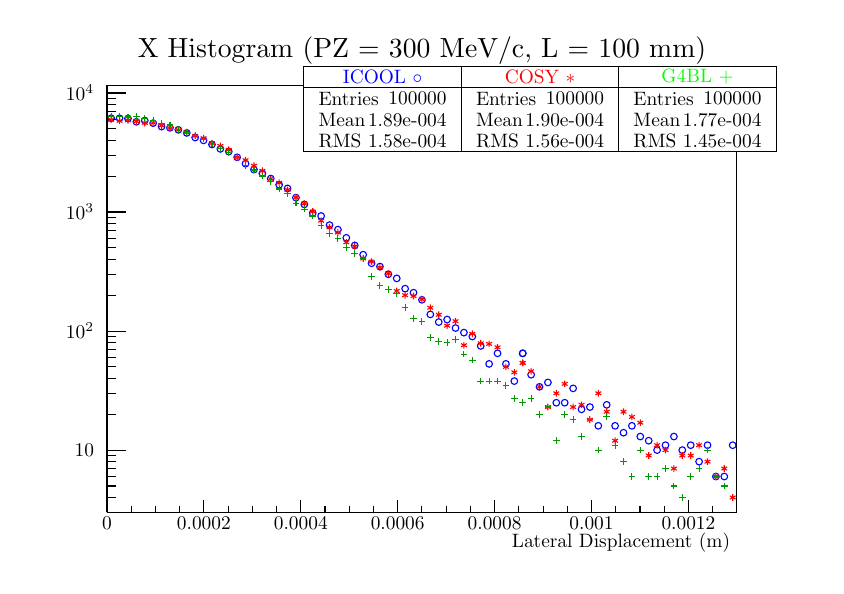
\begin{tikzpicture}
\definecolor{c}{rgb}{1,1,1};
\draw [color=c, fill=c] (0,0) rectangle (20,13.5632);
\draw [color=c, fill=c] (2,1.35632) rectangle (18,12.2069);
\definecolor{c}{rgb}{0,0,0};
\draw [c] (2,1.35632) -- (2,12.2069) -- (18,12.2069) -- (18,1.35632) -- (2,1.35632);
\definecolor{c}{rgb}{1,1,1};
\draw [color=c, fill=c] (2,1.35632) rectangle (18,12.2069);
\definecolor{c}{rgb}{0,0,0};
\draw [c] (2,1.35632) -- (2,12.2069) -- (18,12.2069) -- (18,1.35632) -- (2,1.35632);
\definecolor{c}{rgb}{0,0,1};
\foreach \P in
 {(2.10667,11.3676),(2.32,11.3655),(2.53333,11.3592),(2.74667,11.2763),(2.96,11.3081),(3.17333,11.2426),(3.38667,11.154),(3.6,11.1247),(3.81333,11.073),(4.02667,10.9943),(4.24,10.8775),(4.45333,10.8039),(4.66667,10.7003),(4.88,10.5882),(5.09333,10.51
98),(5.30667,10.3745),(5.52,10.2126),(5.73333,10.0625),(5.94667,9.96655),(6.16,9.83514),(6.37333,9.67676),(6.58667,9.58438),(6.8,9.35092),(7.01333,9.17797),(7.22667,8.95879),(7.44,8.88435),(7.65333,8.65227),(7.86667,8.53738),(8.08,8.3297),(8.29333,8.
1366),(8.50667,7.90116),(8.72,7.68314),(8.93333,7.59909),(9.14667,7.40417),(9.36,7.29942),(9.57333,7.03799),(9.78667,6.93576),(10,6.75502),(10.2133,6.38438),(10.4267,6.18984),(10.64,6.25444),(10.8533,6.03792),(11.0667,5.92139),(11.28,5.82303),(11.493
3,5.58359),(11.7067,5.12762),(11.92,5.39566),(12.1333,5.12762),(12.3467,4.69069),(12.56,5.39566)}{\draw[mark options={color=c,fill=c},mark size=2.402402pt,mark=o] plot coordinates {\P};}
\foreach \P in
 {(12.56,5.39566),(12.7733,4.85303),(12.9867,4.54462),(13.2,4.65567),(13.4133,4.14081),(13.6267,4.14081),(13.84,4.50541),(14.0533,3.97293),(14.2667,4.03131),(14.48,3.55471),(14.6933,4.0872),(14.9067,3.55471),(15.12,3.37935),(15.3333,3.55471),(15.5467
,3.28202),(15.76,3.17691),(15.9733,2.93747),(16.1867,3.06264),(16.4,3.28202),(16.6133,2.93747),(16.8267,3.06264),(17.04,2.64442),(17.2533,3.06264),(17.4667,2.26661),(17.68,2.26661),(17.8933,3.06264)}{\draw[mark options={color=c,fill=c},mark
 size=2.402402pt,mark=o] plot coordinates {\P};}
\definecolor{c}{rgb}{1,1,1};
\draw [color=c, fill=c] (7,10.5115) rectangle (11,12.6816);
\definecolor{c}{rgb}{0,0,0};
\draw [c] (7,10.5115) -- (11,10.5115);
\draw [c] (11,10.5115) -- (11,12.6816);
\draw [c] (11,12.6816) -- (7,12.6816);
\draw [c] (7,12.6816) -- (7,10.5115);
\draw[color=blue](9,12.4103) node[scale=0.7, rotate=0]{ICOOL $\circ$};
\draw [c] (7,12.1391) -- (11,12.1391);
\draw [anchor= west] (7.2,11.8678) node[scale=0.7, rotate=0]{Entries };
\draw [anchor= east] (10.8,11.8678) node[scale=0.7, rotate=0]{ 100000};
\draw [anchor= west] (7.2,11.3253) node[scale=0.7, rotate=0]{Mean  };
\draw [anchor= east] (10.8,11.3253) node[scale=0.7, rotate=0]{ 1.89e-004};
\draw [anchor= west] (7.2,10.7828) node[scale=0.7, rotate=0]{RMS   };
\draw [anchor= east] (10.8,10.7828) node[scale=0.7, rotate=0]{ 1.58e-004};
\draw [c] (2,1.35632) -- (18,1.35632);
\draw [anchor= east] (18,0.596782) node[scale=0.7, rotate=0]{Lateral Displacement (m)};
\draw [c] (2,1.68184) -- (2,1.35632);
\draw [c] (2.61538,1.51908) -- (2.61538,1.35632);
\draw [c] (3.23077,1.51908) -- (3.23077,1.35632);
\draw [c] (3.84615,1.51908) -- (3.84615,1.35632);
\draw [c] (4.46154,1.68184) -- (4.46154,1.35632);
\draw [c] (5.07692,1.51908) -- (5.07692,1.35632);
\draw [c] (5.69231,1.51908) -- (5.69231,1.35632);
\draw [c] (6.30769,1.51908) -- (6.30769,1.35632);
\draw [c] (6.92308,1.68184) -- (6.92308,1.35632);
\draw [c] (7.53846,1.51908) -- (7.53846,1.35632);
\draw [c] (8.15385,1.51908) -- (8.15385,1.35632);
\draw [c] (8.76923,1.51908) -- (8.76923,1.35632);
\draw [c] (9.38461,1.68184) -- (9.38461,1.35632);
\draw [c] (10,1.51908) -- (10,1.35632);
\draw [c] (10.6154,1.51908) -- (10.6154,1.35632);
\draw [c] (11.2308,1.51908) -- (11.2308,1.35632);
\draw [c] (11.8462,1.68184) -- (11.8462,1.35632);
\draw [c] (12.4615,1.51908) -- (12.4615,1.35632);
\draw [c] (13.0769,1.51908) -- (13.0769,1.35632);
\draw [c] (13.6923,1.51908) -- (13.6923,1.35632);
\draw [c] (14.3077,1.68184) -- (14.3077,1.35632);
\draw [c] (14.9231,1.51908) -- (14.9231,1.35632);
\draw [c] (15.5385,1.51908) -- (15.5385,1.35632);
\draw [c] (16.1538,1.51908) -- (16.1538,1.35632);
\draw [c] (16.7692,1.68184) -- (16.7692,1.35632);
\draw [c] (16.7692,1.68184) -- (16.7692,1.35632);
\draw [c] (17.3846,1.51908) -- (17.3846,1.35632);
\draw [c] (18,1.51908) -- (18,1.35632);
\draw [anchor=base] (2,0.908736) node[scale=0.7, rotate=0]{0};
\draw [anchor=base] (4.46154,0.908736) node[scale=0.7, rotate=0]{0.0002};
\draw [anchor=base] (6.92308,0.908736) node[scale=0.7, rotate=0]{0.0004};
\draw [anchor=base] (9.38461,0.908736) node[scale=0.7, rotate=0]{0.0006};
\draw [anchor=base] (11.8462,0.908736) node[scale=0.7, rotate=0]{0.0008};
\draw [anchor=base] (14.3077,0.908736) node[scale=0.7, rotate=0]{0.001};
\draw [anchor=base] (16.7692,0.908736) node[scale=0.7, rotate=0]{0.0012};
\draw [c] (2,1.35632) -- (2,12.2069);
\draw [c] (2.24,1.73412) -- (2,1.73412);
\draw [c] (2.24,2.02717) -- (2,2.02717);
\draw [c] (2.24,2.26661) -- (2,2.26661);
\draw [c] (2.24,2.46905) -- (2,2.46905);
\draw [c] (2.24,2.64442) -- (2,2.64442);
\draw [c] (2.24,2.7991) -- (2,2.7991);
\draw [c] (2.48,2.93747) -- (2,2.93747);
\draw [anchor= east] (1.844,2.93747) node[scale=0.7, rotate=0]{10};
\draw [c] (2.24,3.84776) -- (2,3.84776);
\draw [c] (2.24,4.38024) -- (2,4.38024);
\draw [c] (2.24,4.75805) -- (2,4.75805);
\draw [c] (2.24,5.0511) -- (2,5.0511);
\draw [c] (2.24,5.29054) -- (2,5.29054);
\draw [c] (2.24,5.49298) -- (2,5.49298);
\draw [c] (2.24,5.66834) -- (2,5.66834);
\draw [c] (2.24,5.82302) -- (2,5.82302);
\draw [c] (2.48,5.96139) -- (2,5.96139);
\draw [anchor= east] (1.844,5.96139) node[scale=0.7, rotate=0]{$10^{2}$};
\draw [c] (2.24,6.87168) -- (2,6.87168);
\draw [c] (2.24,7.40417) -- (2,7.40417);
\draw [c] (2.24,7.78198) -- (2,7.78198);
\draw [c] (2.24,8.07502) -- (2,8.07502);
\draw [c] (2.24,8.31446) -- (2,8.31446);
\draw [c] (2.24,8.5169) -- (2,8.5169);
\draw [c] (2.24,8.69227) -- (2,8.69227);
\draw [c] (2.24,8.84695) -- (2,8.84695);
\draw [c] (2.48,8.98532) -- (2,8.98532);
\draw [anchor= east] (1.844,8.98532) node[scale=0.7, rotate=0]{$10^{3}$};
\draw [c] (2.24,9.89561) -- (2,9.89561);
\draw [c] (2.24,10.4281) -- (2,10.4281);
\draw [c] (2.24,10.8059) -- (2,10.8059);
\draw [c] (2.24,11.0989) -- (2,11.0989);
\draw [c] (2.24,11.3384) -- (2,11.3384);
\draw [c] (2.24,11.5408) -- (2,11.5408);
\draw [c] (2.24,11.7162) -- (2,11.7162);
\draw [c] (2.24,11.8709) -- (2,11.8709);
\draw [c] (2.48,12.0092) -- (2,12.0092);
\draw [anchor= east] (1.844,12.0092) node[scale=0.7, rotate=0]{$10^{4}$};
\definecolor{c}{rgb}{1,1,1};
\draw [color=c, fill=c] (7,10.5115) rectangle (11,12.6816);
\definecolor{c}{rgb}{0,0,0};
\draw [c] (7,10.5115) -- (11,10.5115);
\draw [c] (11,10.5115) -- (11,12.6816);
\draw [c] (11,12.6816) -- (7,12.6816);
\draw [c] (7,12.6816) -- (7,10.5115);
\draw[color=blue](9,12.4103) node[scale=0.7, rotate=0]{ICOOL $\circ$};
\draw [c] (7,12.1391) -- (11,12.1391);
\draw [anchor= west] (7.2,11.8678) node[scale=0.7, rotate=0]{Entries };
\draw [anchor= east] (10.8,11.8678) node[scale=0.7, rotate=0]{ 100000};
\draw [anchor= west] (7.2,11.3253) node[scale=0.7, rotate=0]{Mean  };
\draw [anchor= east] (10.8,11.3253) node[scale=0.7, rotate=0]{ 1.89e-004};
\draw [anchor= west] (7.2,10.7828) node[scale=0.7, rotate=0]{RMS   };
\draw [anchor= east] (10.8,10.7828) node[scale=0.7, rotate=0]{ 1.58e-004};
\draw (10,13.0816) node[scale=1, rotate=0]{X Histogram (PZ = 300 MeV/c, L = 100 mm)};
\definecolor{c}{rgb}{1,0,0};
\foreach \P in
 {(2.10667,11.3267),(2.32,11.2991),(2.53333,11.3127),(2.74667,11.2882),(2.96,11.2473),(3.17333,11.2485),(3.38667,11.1817),(3.6,11.1172),(3.81333,11.0692),(4.02667,11.0096),(4.24,10.9188),(4.45333,10.8606),(4.66667,10.734),(4.88,10.6635),(5.09333,10.5
667),(5.30667,10.3772),(5.52,10.3009),(5.73333,10.1594),(5.94667,10.0315),(6.16,9.82548),(6.37333,9.72997),(6.58667,9.54638),(6.8,9.35489),(7.01333,9.19711),(7.22667,8.99838),(7.44,8.76569),(7.65333,8.5952),(7.86667,8.46525),(8.08,8.21444),(8.29333,8
.11129),(8.50667,7.80476),(8.72,7.72494),(8.93333,7.57625),(9.14667,7.42157),(9.36,6.97882),(9.57333,6.87168),(9.78667,6.85184),(10,6.7693),(10.2133,6.55378),(10.4267,6.37483),(10.64,6.09845),(10.8533,6.21173),(11.0667,5.60098),(11.28,5.89403),(11.49
33,5.65182),(11.7067,5.63509),(11.92,5.54809),(12.1333,5.0511),(12.3467,4.91273),(12.56,5.15217)}{\draw[mark options={color=c,fill=c},mark size=2.402402pt,mark=asterisk] plot coordinates {\P};}
\foreach \P in
 {(12.56,5.15217),(12.7733,4.9416),(12.9867,4.54462),(13.2,4.03131),(13.4133,4.38025),(13.6267,4.61968),(13.84,4.03131),(14.0533,4.0872),(14.2667,3.70939),(14.48,4.38025),(14.6933,3.91183),(14.9067,3.17691),(15.12,3.91183),(15.3333,3.7804),(15.5467,3
.63433),(15.76,2.7991),(15.9733,3.06264),(16.1867,2.93747),(16.4,2.46906),(16.6133,2.7991),(16.8267,2.7991),(17.04,3.06264),(17.2533,2.64442),(17.4667,2.26661),(17.68,2.46906),(17.8933,1.73413)}{\draw[mark options={color=c,fill=c},mark
 size=2.402402pt,mark=asterisk] plot coordinates {\P};}
\definecolor{c}{rgb}{1,1,1};
\draw [color=c, fill=c] (11,10.5115) rectangle (15,12.6816);
\definecolor{c}{rgb}{0,0,0};
\draw [c] (11,10.5115) -- (15,10.5115);
\draw [c] (15,10.5115) -- (15,12.6816);
\draw [c] (15,12.6816) -- (11,12.6816);
\draw [c] (11,12.6816) -- (11,10.5115);
\draw [color=red](13,12.4103) node[scale=0.7, rotate=0]{COSY $*$};
\draw [c] (11,12.1391) -- (15,12.1391);
\draw [anchor= west] (11.2,11.8678) node[scale=0.7, rotate=0]{Entries };
\draw [anchor= east] (14.8,11.8678) node[scale=0.7, rotate=0]{ 100000};
\draw [anchor= west] (11.2,11.3253) node[scale=0.7, rotate=0]{Mean  };
\draw [anchor= east] (14.8,11.3253) node[scale=0.7, rotate=0]{ 1.90e-004};
\draw [anchor= west] (11.2,10.7828) node[scale=0.7, rotate=0]{RMS   };
\draw [anchor= east] (14.8,10.7828) node[scale=0.7, rotate=0]{ 1.56e-004};
\definecolor{c}{rgb}{1,1,1};
\draw [color=c, fill=c] (11,10.5115) rectangle (15,12.6816);
\definecolor{c}{rgb}{0,0,0};
\draw [c] (11,10.5115) -- (15,10.5115);
\draw [c] (15,10.5115) -- (15,12.6816);
\draw [c] (15,12.6816) -- (11,12.6816);
\draw [c] (11,12.6816) -- (11,10.5115);
\draw [color=red](13,12.4103) node[scale=0.7, rotate=0]{COSY $*$};
\draw [c] (11,12.1391) -- (15,12.1391);
\draw [anchor= west] (11.2,11.8678) node[scale=0.7, rotate=0]{Entries };
\draw [anchor= east] (14.8,11.8678) node[scale=0.7, rotate=0]{ 100000};
\draw [anchor= west] (11.2,11.3253) node[scale=0.7, rotate=0]{Mean  };
\draw [anchor= east] (14.8,11.3253) node[scale=0.7, rotate=0]{ 1.90e-004};
\draw [anchor= west] (11.2,10.7828) node[scale=0.7, rotate=0]{RMS   };
\draw [anchor= east] (14.8,10.7828) node[scale=0.7, rotate=0]{ 1.56e-004};
\definecolor{c}{rgb}{0,0.6,0};
\foreach \P in
 {(2.10667,11.4102),(2.32,11.417),(2.53333,11.3983),(2.74667,11.4133),(2.96,11.3577),(3.17333,11.3076),(3.38667,11.241),(3.6,11.1939),(3.81333,11.0823),(4.02667,11.0051),(4.24,10.9251),(4.45333,10.837),(4.66667,10.7152),(4.88,10.6006),(5.09333,10.504
2),(5.30667,10.3676),(5.52,10.1659),(5.73333,10.0515),(5.94667,9.9002),(6.16,9.75212),(6.37333,9.57015),(6.58667,9.45136),(6.8,9.21045),(7.01333,9.05936),(7.22667,8.88435),(7.44,8.63866),(7.65333,8.42964),(7.86667,8.30788),(8.08,8.08549),(8.29333,7.9
2493),(8.50667,7.80153),(8.72,7.34141),(8.93333,7.11112),(9.14667,7.01464),(9.36,6.90411),(9.57333,6.56212),(9.78667,6.27529),(10,6.20083),(10.2133,5.79351),(10.4267,5.70077),(10.64,5.66834),(10.8533,5.74796),(11.0667,5.3753),(11.28,5.22318),(11.4933
,4.69069),(11.7067,4.69069),(11.92,4.69069),(12.1333,4.58269),(12.3467,4.24188),(12.56,4.14081)}{\draw[mark options={color=c,fill=c},mark size=2.402402pt,mark=+] plot coordinates {\P};}
\foreach \P in
 {(12.56,4.14081),(12.7733,4.24188),(12.9867,3.84776),(13.2,4.03131),(13.4133,3.17691),(13.6267,3.84776),(13.84,3.70939),(14.0533,3.28202),(14.2667,3.70939),(14.48,2.93747),(14.6933,3.7804),(14.9067,3.06264),(15.12,2.64442),(15.3333,2.26661),(15.5467
,2.93747),(15.76,2.26661),(15.9733,2.26661),(16.1867,2.46906),(16.4,2.02718),(16.6133,1.73413),(16.8267,2.26661),(17.04,2.46906),(17.2533,2.93747),(17.4667,2.26661),(17.68,2.02718)}{\draw[mark options={color=c,fill=c},mark size=2.402402pt,mark=+]
 plot coordinates {\P};}
\definecolor{c}{rgb}{1,1,1};
\draw [color=c, fill=c] (15,10.5115) rectangle (19,12.6816);
\definecolor{c}{rgb}{0,0,0};
\draw [c] (15,10.5115) -- (19,10.5115);
\draw [c] (19,10.5115) -- (19,12.6816);
\draw [c] (19,12.6816) -- (15,12.6816);
\draw [c] (15,12.6816) -- (15,10.5115);
\draw [color=green](17,12.4103) node[scale=0.7, rotate=0]{G4BL $+$};
\draw [c] (15,12.1391) -- (19,12.1391);
\draw [anchor= west] (15.2,11.8678) node[scale=0.7, rotate=0]{Entries };
\draw [anchor= east] (18.8,11.8678) node[scale=0.7, rotate=0]{ 100000};
\draw [anchor= west] (15.2,11.3253) node[scale=0.7, rotate=0]{Mean  };
\draw [anchor= east] (18.8,11.3253) node[scale=0.7, rotate=0]{ 1.77e-004};
\draw [anchor= west] (15.2,10.7828) node[scale=0.7, rotate=0]{RMS   };
\draw [anchor= east] (18.8,10.7828) node[scale=0.7, rotate=0]{ 1.45e-004};
\definecolor{c}{rgb}{1,1,1};
\draw [color=c, fill=c] (15,10.5115) rectangle (19,12.6816);
\definecolor{c}{rgb}{0,0,0};
\draw [c] (15,10.5115) -- (19,10.5115);
\draw [c] (19,10.5115) -- (19,12.6816);
\draw [c] (19,12.6816) -- (15,12.6816);
\draw [c] (15,12.6816) -- (15,10.5115);
\draw [color=green](17,12.4103) node[scale=0.7, rotate=0]{G4BL $+$};
\draw [c] (15,12.1391) -- (19,12.1391);
\draw [anchor= west] (15.2,11.8678) node[scale=0.7, rotate=0]{Entries };
\draw [anchor= east] (18.8,11.8678) node[scale=0.7, rotate=0]{ 100000};
\draw [anchor= west] (15.2,11.3253) node[scale=0.7, rotate=0]{Mean  };
\draw [anchor= east] (18.8,11.3253) node[scale=0.7, rotate=0]{ 1.77e-004};
\draw [anchor= west] (15.2,10.7828) node[scale=0.7, rotate=0]{RMS   };
\draw [anchor= east] (18.8,10.7828) node[scale=0.7, rotate=0]{ 1.45e-004};
\end{tikzpicture}
}\\
\frame{    \pgfdeclareplotmark{cross} {
\pgfpathmoveto{\pgfpoint{-0.3\pgfplotmarksize}{\pgfplotmarksize}}
\pgfpathlineto{\pgfpoint{+0.3\pgfplotmarksize}{\pgfplotmarksize}}
\pgfpathlineto{\pgfpoint{+0.3\pgfplotmarksize}{0.3\pgfplotmarksize}}
\pgfpathlineto{\pgfpoint{+1\pgfplotmarksize}{0.3\pgfplotmarksize}}
\pgfpathlineto{\pgfpoint{+1\pgfplotmarksize}{-0.3\pgfplotmarksize}}
\pgfpathlineto{\pgfpoint{+0.3\pgfplotmarksize}{-0.3\pgfplotmarksize}}
\pgfpathlineto{\pgfpoint{+0.3\pgfplotmarksize}{-1.\pgfplotmarksize}}
\pgfpathlineto{\pgfpoint{-0.3\pgfplotmarksize}{-1.\pgfplotmarksize}}
\pgfpathlineto{\pgfpoint{-0.3\pgfplotmarksize}{-0.3\pgfplotmarksize}}
\pgfpathlineto{\pgfpoint{-1.\pgfplotmarksize}{-0.3\pgfplotmarksize}}
\pgfpathlineto{\pgfpoint{-1.\pgfplotmarksize}{0.3\pgfplotmarksize}}
\pgfpathlineto{\pgfpoint{-0.3\pgfplotmarksize}{0.3\pgfplotmarksize}}
\pgfpathclose
\pgfusepathqstroke
}
\pgfdeclareplotmark{cross*} {
\pgfpathmoveto{\pgfpoint{-0.3\pgfplotmarksize}{\pgfplotmarksize}}
\pgfpathlineto{\pgfpoint{+0.3\pgfplotmarksize}{\pgfplotmarksize}}
\pgfpathlineto{\pgfpoint{+0.3\pgfplotmarksize}{0.3\pgfplotmarksize}}
\pgfpathlineto{\pgfpoint{+1\pgfplotmarksize}{0.3\pgfplotmarksize}}
\pgfpathlineto{\pgfpoint{+1\pgfplotmarksize}{-0.3\pgfplotmarksize}}
\pgfpathlineto{\pgfpoint{+0.3\pgfplotmarksize}{-0.3\pgfplotmarksize}}
\pgfpathlineto{\pgfpoint{+0.3\pgfplotmarksize}{-1.\pgfplotmarksize}}
\pgfpathlineto{\pgfpoint{-0.3\pgfplotmarksize}{-1.\pgfplotmarksize}}
\pgfpathlineto{\pgfpoint{-0.3\pgfplotmarksize}{-0.3\pgfplotmarksize}}
\pgfpathlineto{\pgfpoint{-1.\pgfplotmarksize}{-0.3\pgfplotmarksize}}
\pgfpathlineto{\pgfpoint{-1.\pgfplotmarksize}{0.3\pgfplotmarksize}}
\pgfpathlineto{\pgfpoint{-0.3\pgfplotmarksize}{0.3\pgfplotmarksize}}
\pgfpathclose
\pgfusepathqfillstroke
}
\pgfdeclareplotmark{newstar} {
\pgfpathmoveto{\pgfqpoint{0pt}{\pgfplotmarksize}}
\pgfpathlineto{\pgfqpointpolar{44}{0.5\pgfplotmarksize}}
\pgfpathlineto{\pgfqpointpolar{18}{\pgfplotmarksize}}
\pgfpathlineto{\pgfqpointpolar{-20}{0.5\pgfplotmarksize}}
\pgfpathlineto{\pgfqpointpolar{-54}{\pgfplotmarksize}}
\pgfpathlineto{\pgfqpointpolar{-90}{0.5\pgfplotmarksize}}
\pgfpathlineto{\pgfqpointpolar{234}{\pgfplotmarksize}}
\pgfpathlineto{\pgfqpointpolar{198}{0.5\pgfplotmarksize}}
\pgfpathlineto{\pgfqpointpolar{162}{\pgfplotmarksize}}
\pgfpathlineto{\pgfqpointpolar{134}{0.5\pgfplotmarksize}}
\pgfpathclose
\pgfusepathqstroke
}
\pgfdeclareplotmark{newstar*} {
\pgfpathmoveto{\pgfqpoint{0pt}{\pgfplotmarksize}}
\pgfpathlineto{\pgfqpointpolar{44}{0.5\pgfplotmarksize}}
\pgfpathlineto{\pgfqpointpolar{18}{\pgfplotmarksize}}
\pgfpathlineto{\pgfqpointpolar{-20}{0.5\pgfplotmarksize}}
\pgfpathlineto{\pgfqpointpolar{-54}{\pgfplotmarksize}}
\pgfpathlineto{\pgfqpointpolar{-90}{0.5\pgfplotmarksize}}
\pgfpathlineto{\pgfqpointpolar{234}{\pgfplotmarksize}}
\pgfpathlineto{\pgfqpointpolar{198}{0.5\pgfplotmarksize}}
\pgfpathlineto{\pgfqpointpolar{162}{\pgfplotmarksize}}
\pgfpathlineto{\pgfqpointpolar{134}{0.5\pgfplotmarksize}}
\pgfpathclose
\pgfusepathqfillstroke
}
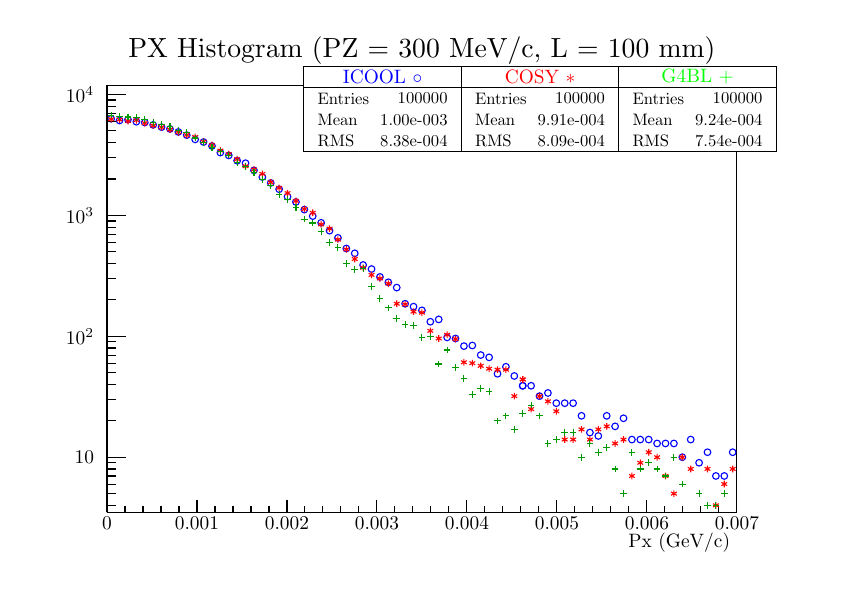
\begin{tikzpicture}
\definecolor{c}{rgb}{1,1,1};
\draw [color=c, fill=c] (0,0) rectangle (20,13.5632);
\draw [color=c, fill=c] (2,1.35632) rectangle (18,12.2069);
\definecolor{c}{rgb}{0,0,0};
\draw [c] (2,1.35632) -- (2,12.2069) -- (18,12.2069) -- (18,1.35632) -- (2,1.35632);
\definecolor{c}{rgb}{1,1,1};
\draw [color=c, fill=c] (2,1.35632) rectangle (18,12.2069);
\definecolor{c}{rgb}{0,0,0};
\draw [c] (2,1.35632) -- (2,12.2069) -- (18,12.2069) -- (18,1.35632) -- (2,1.35632);
\definecolor{c}{rgb}{0,0,1};
\foreach \P in
 {(2.10667,11.3545),(2.32,11.31),(2.53333,11.3334),(2.74667,11.2782),(2.96,11.259),(3.17333,11.1979),(3.38667,11.1407),(3.6,11.0953),(3.81333,11.0186),(4.02667,10.9376),(4.24,10.8302),(4.45333,10.7627),(4.66667,10.6613),(4.88,10.4945),(5.09333,10.422
4),(5.30667,10.2873),(5.52,10.2252),(5.73333,10.042),(5.94667,9.87399),(6.16,9.7233),(6.37333,9.56396),(6.58667,9.37647),(6.8,9.24018),(7.01333,9.04607),(7.22667,8.88104),(7.44,8.71123),(7.65333,8.51125),(7.86667,8.32805),(8.08,8.05927),(8.29333,7.93
616),(8.50667,7.63923),(8.72,7.5359),(8.93333,7.33647),(9.14667,7.20072),(9.36,7.06548),(9.57333,6.65517),(9.78667,6.58146),(10,6.48728),(10.2133,6.19778),(10.4267,6.25706),(10.64,5.80055),(10.8533,5.77305),(11.0667,5.57898),(11.28,5.59495),(11.4933,
5.35179),(11.7067,5.29337),(11.92,4.87608),(12.1333,5.05418),(12.3467,4.8205),(12.56,4.57165)}{\draw[mark options={color=c,fill=c},mark size=2.402402pt,mark=o] plot coordinates {\P};}
\foreach \P in
 {(12.56,4.57165),(12.7733,4.57165),(12.9867,4.30781),(13.2,4.38866),(13.4133,4.12971),(13.6267,4.12971),(13.84,4.12971),(14.0533,3.80807),(14.2667,3.38334),(14.48,3.29727),(14.6933,3.80807),(14.9067,3.54043),(15.12,3.74603),(15.3333,3.20525),(15.546
7,3.20525),(15.76,3.20525),(15.9733,3.10641),(16.1867,3.10641),(16.4,3.10641),(16.6133,2.75649),(16.8267,3.20525),(17.04,2.61597),(17.2533,2.88361),(17.4667,2.28079),(17.68,2.28079),(17.8933,2.88361)}{\draw[mark options={color=c,fill=c},mark
 size=2.402402pt,mark=o] plot coordinates {\P};}
\definecolor{c}{rgb}{1,1,1};
\draw [color=c, fill=c] (7,10.5115) rectangle (11,12.6816);
\definecolor{c}{rgb}{0,0,0};
\draw [c] (7,10.5115) -- (11,10.5115);
\draw [c] (11,10.5115) -- (11,12.6816);
\draw [c] (11,12.6816) -- (7,12.6816);
\draw [c] (7,12.6816) -- (7,10.5115);
\draw[color=blue](9,12.4103) node[scale=0.7, rotate=0]{ICOOL $\circ$};
\draw [c] (7,12.1391) -- (11,12.1391);
\draw [anchor= west] (7.2,11.8678) node[scale=0.6, rotate=0]{Entries };
\draw [anchor= east] (10.8,11.8678) node[scale=0.6, rotate=0]{ 100000};
\draw [anchor= west] (7.2,11.3253) node[scale=0.6, rotate=0]{Mean  };
\draw [anchor= east] (10.8,11.3253) node[scale=0.6, rotate=0]{ 1.00e-003};
\draw [anchor= west] (7.2,10.7828) node[scale=0.6, rotate=0]{RMS   };
\draw [anchor= east] (10.8,10.7828) node[scale=0.6, rotate=0]{ 8.38e-004};
\draw [c] (2,1.35632) -- (18,1.35632);
\draw [anchor= east] (18,0.596782) node[scale=0.7, rotate=0]{Px (GeV/c)};
\draw [c] (2,1.68184) -- (2,1.35632);
\draw [c] (2.45714,1.51908) -- (2.45714,1.35632);
\draw [c] (2.91429,1.51908) -- (2.91429,1.35632);
\draw [c] (3.37143,1.51908) -- (3.37143,1.35632);
\draw [c] (3.82857,1.51908) -- (3.82857,1.35632);
\draw [c] (4.28571,1.68184) -- (4.28571,1.35632);
\draw [c] (4.74286,1.51908) -- (4.74286,1.35632);
\draw [c] (5.2,1.51908) -- (5.2,1.35632);
\draw [c] (5.65714,1.51908) -- (5.65714,1.35632);
\draw [c] (6.11429,1.51908) -- (6.11429,1.35632);
\draw [c] (6.57143,1.68184) -- (6.57143,1.35632);
\draw [c] (7.02857,1.51908) -- (7.02857,1.35632);
\draw [c] (7.48571,1.51908) -- (7.48571,1.35632);
\draw [c] (7.94286,1.51908) -- (7.94286,1.35632);
\draw [c] (8.4,1.51908) -- (8.4,1.35632);
\draw [c] (8.85714,1.68184) -- (8.85714,1.35632);
\draw [c] (9.31429,1.51908) -- (9.31429,1.35632);
\draw [c] (9.77143,1.51908) -- (9.77143,1.35632);
\draw [c] (10.2286,1.51908) -- (10.2286,1.35632);
\draw [c] (10.6857,1.51908) -- (10.6857,1.35632);
\draw [c] (11.1429,1.68184) -- (11.1429,1.35632);
\draw [c] (11.6,1.51908) -- (11.6,1.35632);
\draw [c] (12.0571,1.51908) -- (12.0571,1.35632);
\draw [c] (12.5143,1.51908) -- (12.5143,1.35632);
\draw [c] (12.9714,1.51908) -- (12.9714,1.35632);
\draw [c] (13.4286,1.68184) -- (13.4286,1.35632);
\draw [c] (13.8857,1.51908) -- (13.8857,1.35632);
\draw [c] (14.3429,1.51908) -- (14.3429,1.35632);
\draw [c] (14.8,1.51908) -- (14.8,1.35632);
\draw [c] (15.2571,1.51908) -- (15.2571,1.35632);
\draw [c] (15.7143,1.68184) -- (15.7143,1.35632);
\draw [c] (16.1714,1.51908) -- (16.1714,1.35632);
\draw [c] (16.6286,1.51908) -- (16.6286,1.35632);
\draw [c] (17.0857,1.51908) -- (17.0857,1.35632);
\draw [c] (17.5429,1.51908) -- (17.5429,1.35632);
\draw [c] (18,1.68184) -- (18,1.35632);
\draw [c] (18,1.68184) -- (18,1.35632);
\draw [anchor=base] (2,0.908736) node[scale=0.7, rotate=0]{0};
\draw [anchor=base] (4.28571,0.908736) node[scale=0.7, rotate=0]{0.001};
\draw [anchor=base] (6.57143,0.908736) node[scale=0.7, rotate=0]{0.002};
\draw [anchor=base] (8.85714,0.908736) node[scale=0.7, rotate=0]{0.003};
\draw [anchor=base] (11.1429,0.908736) node[scale=0.7, rotate=0]{0.004};
\draw [anchor=base] (13.4286,0.908736) node[scale=0.7, rotate=0]{0.005};
\draw [anchor=base] (15.7143,0.908736) node[scale=0.7, rotate=0]{0.006};
\draw [anchor=base] (18,0.908736) node[scale=0.7, rotate=0]{0.007};
\draw [c] (2,1.35632) -- (2,12.2069);
\draw [c] (2.24,1.53441) -- (2,1.53441);
\draw [c] (2.24,1.83202) -- (2,1.83202);
\draw [c] (2.24,2.07519) -- (2,2.07519);
\draw [c] (2.24,2.28078) -- (2,2.28078);
\draw [c] (2.24,2.45888) -- (2,2.45888);
\draw [c] (2.24,2.61597) -- (2,2.61597);
\draw [c] (2.48,2.75649) -- (2,2.75649);
\draw [anchor= east] (1.844,2.75649) node[scale=0.7, rotate=0]{10};
\draw [c] (2.24,3.68095) -- (2,3.68095);
\draw [c] (2.24,4.22173) -- (2,4.22173);
\draw [c] (2.24,4.60542) -- (2,4.60542);
\draw [c] (2.24,4.90303) -- (2,4.90303);
\draw [c] (2.24,5.14619) -- (2,5.14619);
\draw [c] (2.24,5.35179) -- (2,5.35179);
\draw [c] (2.24,5.52988) -- (2,5.52988);
\draw [c] (2.24,5.68697) -- (2,5.68697);
\draw [c] (2.48,5.82749) -- (2,5.82749);
\draw [anchor= east] (1.844,5.82749) node[scale=0.7, rotate=0]{$10^{2}$};
\draw [c] (2.24,6.75196) -- (2,6.75196);
\draw [c] (2.24,7.29273) -- (2,7.29273);
\draw [c] (2.24,7.67642) -- (2,7.67642);
\draw [c] (2.24,7.97403) -- (2,7.97403);
\draw [c] (2.24,8.2172) -- (2,8.2172);
\draw [c] (2.24,8.42279) -- (2,8.42279);
\draw [c] (2.24,8.60088) -- (2,8.60088);
\draw [c] (2.24,8.75797) -- (2,8.75797);
\draw [c] (2.48,8.89849) -- (2,8.89849);
\draw [anchor= east] (1.844,8.89849) node[scale=0.7, rotate=0]{$10^{3}$};
\draw [c] (2.24,9.82296) -- (2,9.82296);
\draw [c] (2.24,10.3637) -- (2,10.3637);
\draw [c] (2.24,10.7474) -- (2,10.7474);
\draw [c] (2.24,11.045) -- (2,11.045);
\draw [c] (2.24,11.2882) -- (2,11.2882);
\draw [c] (2.24,11.4938) -- (2,11.4938);
\draw [c] (2.24,11.6719) -- (2,11.6719);
\draw [c] (2.24,11.829) -- (2,11.829);
\draw [c] (2.48,11.9695) -- (2,11.9695);
\draw [anchor= east] (1.844,11.9695) node[scale=0.7, rotate=0]{$10^{4}$};
\definecolor{c}{rgb}{1,1,1};
\draw [color=c, fill=c] (7,10.5115) rectangle (11,12.6816);
\definecolor{c}{rgb}{0,0,0};
\draw [c] (7,10.5115) -- (11,10.5115);
\draw [c] (11,10.5115) -- (11,12.6816);
\draw [c] (11,12.6816) -- (7,12.6816);
\draw [c] (7,12.6816) -- (7,10.5115);
\draw[color=blue](9,12.4103) node[scale=0.7, rotate=0]{ICOOL $\circ$};
\draw [c] (7,12.1391) -- (11,12.1391);
\draw [anchor= west] (7.2,11.8678) node[scale=0.6, rotate=0]{Entries };
\draw [anchor= east] (10.8,11.8678) node[scale=0.6, rotate=0]{ 100000};
\draw [anchor= west] (7.2,11.3253) node[scale=0.6, rotate=0]{Mean  };
\draw [anchor= east] (10.8,11.3253) node[scale=0.6, rotate=0]{ 1.00e-003};
\draw [anchor= west] (7.2,10.7828) node[scale=0.6, rotate=0]{RMS   };
\draw [anchor= east] (10.8,10.7828) node[scale=0.6, rotate=0]{ 8.38e-004};
\draw (10,13.0816) node[scale=1, rotate=0]{PX Histogram (PZ = 300 MeV/c, L = 100 mm)};
\definecolor{c}{rgb}{1,0,0};
\foreach \P in
 {(2.10667,11.3431),(2.32,11.3319),(2.53333,11.2942),(2.74667,11.3172),(2.96,11.2439),(3.17333,11.1809),(3.38667,11.1388),(3.6,11.0787),(3.81333,11.0115),(4.02667,10.9408),(4.24,10.8914),(4.45333,10.7732),(4.66667,10.6853),(4.88,10.5459),(5.09333,10.
4552),(5.30667,10.3281),(5.52,10.1475),(5.73333,10.0628),(5.94667,9.9531),(6.16,9.73902),(6.37333,9.59834),(6.58667,9.46481),(6.8,9.26676),(7.01333,9.06032),(7.22667,8.96484),(7.44,8.67071),(7.65333,8.56369),(7.86667,8.28439),(8.08,8.03656),(8.29333,
7.79136),(8.50667,7.56883),(8.72,7.38712),(8.93333,7.29717),(9.14667,7.16695),(9.36,6.65517),(9.57333,6.64075),(9.78667,6.45435),(10,6.4291),(10.2133,5.96668),(10.4267,5.77305),(10.64,5.86692),(10.8533,5.75908),(11.0667,5.16824),(11.28,5.14619),(11.4
933,5.07778),(11.7067,5.00567),(11.92,4.98074),(12.1333,4.98074),(12.3467,4.30781),(12.56,4.73254)}{\draw[mark options={color=c,fill=c},mark size=2.402402pt,mark=asterisk] plot coordinates {\P};}
\foreach \P in
 {(12.56,4.73254),(12.7733,3.97857),(12.9867,4.30781),(13.2,4.17652),(13.4133,3.92412),(13.6267,3.20525),(13.84,3.20525),(14.0533,3.4642),(14.2667,3.20525),(14.48,3.4642),(14.6933,3.54043),(14.9067,3.10641),(15.12,3.20525),(15.3333,2.28079),(15.5467,
2.61597),(15.76,2.88361),(15.9733,2.75649),(16.1867,2.28079),(16.4,1.83203),(16.6133,2.75649),(16.8267,2.45888),(17.2533,2.45888),(17.4667,1.53442),(17.68,2.07519),(17.8933,2.45888)}{\draw[mark options={color=c,fill=c},mark
 size=2.402402pt,mark=asterisk] plot coordinates {\P};}
\definecolor{c}{rgb}{1,1,1};
\draw [color=c, fill=c] (11,10.5115) rectangle (15,12.6816);
\definecolor{c}{rgb}{0,0,0};
\draw [c] (11,10.5115) -- (15,10.5115);
\draw [c] (15,10.5115) -- (15,12.6816);
\draw [c] (15,12.6816) -- (11,12.6816);
\draw [c] (11,12.6816) -- (11,10.5115);
\draw [color=red](13,12.4103) node[scale=0.7, rotate=0]{COSY $*$};
\draw [c] (11,12.1391) -- (15,12.1391);
\draw [anchor= west] (11.2,11.8678) node[scale=0.6, rotate=0]{Entries };
\draw [anchor= east] (14.8,11.8678) node[scale=0.6, rotate=0]{ 100000};
\draw [anchor= west] (11.2,11.3253) node[scale=0.6, rotate=0]{Mean  };
\draw [anchor= east] (14.8,11.3253) node[scale=0.6, rotate=0]{ 9.91e-004};
\draw [anchor= west] (11.2,10.7828) node[scale=0.6, rotate=0]{RMS   };
\draw [anchor= east] (14.8,10.7828) node[scale=0.6, rotate=0]{ 8.09e-004};
\definecolor{c}{rgb}{1,1,1};
\draw [color=c, fill=c] (11,10.5115) rectangle (15,12.6816);
\definecolor{c}{rgb}{0,0,0};
\draw [c] (11,10.5115) -- (15,10.5115);
\draw [c] (15,10.5115) -- (15,12.6816);
\draw [c] (15,12.6816) -- (11,12.6816);
\draw [c] (11,12.6816) -- (11,10.5115);
\draw [color=red](13,12.4103) node[scale=0.7, rotate=0]{COSY $*$};
\draw [c] (11,12.1391) -- (15,12.1391);
\draw [anchor= west] (11.2,11.8678) node[scale=0.6, rotate=0]{Entries };
\draw [anchor= east] (14.8,11.8678) node[scale=0.6, rotate=0]{ 100000};
\draw [anchor= west] (11.2,11.3253) node[scale=0.6, rotate=0]{Mean  };
\draw [anchor= east] (14.8,11.3253) node[scale=0.6, rotate=0]{ 9.91e-004};
\draw [anchor= west] (11.2,10.7828) node[scale=0.6, rotate=0]{RMS   };
\draw [anchor= east] (14.8,10.7828) node[scale=0.6, rotate=0]{ 8.09e-004};
\definecolor{c}{rgb}{0,0.6,0};
\foreach \P in
 {(2.10667,11.4461),(2.32,11.4082),(2.53333,11.397),(2.74667,11.3809),(2.96,11.327),(3.17333,11.2647),(3.38667,11.2052),(3.6,11.1583),(3.81333,11.0501),(4.02667,11.008),(4.24,10.8657),(4.45333,10.7584),(4.66667,10.6289),(4.88,10.5145),(5.09333,10.430
9),(5.30667,10.2472),(5.52,10.1365),(5.73333,9.98537),(5.94667,9.80483),(6.16,9.64715),(6.37333,9.42587),(6.58667,9.30761),(6.8,9.10447),(7.01333,8.80457),(7.22667,8.70661),(7.44,8.48786),(7.65333,8.21497),(7.86667,8.07668),(8.08,7.67975),(8.29333,7.
53219),(8.50667,7.54329),(8.72,7.09158),(8.93333,6.79138),(9.14667,6.5508),(9.36,6.28575),(9.57333,6.13573),(9.78667,6.10359),(10,5.80055),(10.2133,5.81409),(10.4267,5.12378),(10.64,5.47891),(10.8533,5.03015),(11.0667,4.76251),(11.28,4.34885),(11.493
3,4.50144),(11.7067,4.42732),(11.92,3.68095),(12.1333,3.80807),(12.3467,3.4642),(12.56,3.86736)}{\draw[mark options={color=c,fill=c},mark size=2.402402pt,mark=+] plot coordinates {\P};}
\foreach \P in
 {(12.56,3.86736),(12.7733,4.08121),(12.9867,3.80807),(13.2,3.10641),(13.4133,3.20525),(13.6267,3.38334),(13.84,3.38334),(14.0533,2.75649),(14.2667,3.10641),(14.48,2.88361),(14.6933,2.99966),(14.9067,2.45888),(15.12,1.83203),(15.3333,2.88361),(15.546
7,2.45888),(15.76,2.61597),(15.9733,2.45888),(16.1867,2.28079),(16.4,2.75649),(16.6133,2.07519),(17.04,1.83203),(17.2533,1.53442),(17.4667,1.53442),(17.68,1.83203)}{\draw[mark options={color=c,fill=c},mark size=2.402402pt,mark=+] plot coordinates
 {\P};}
\definecolor{c}{rgb}{1,1,1};
\draw [color=c, fill=c] (15,10.5115) rectangle (19,12.6816);
\definecolor{c}{rgb}{0,0,0};
\draw [c] (15,10.5115) -- (19,10.5115);
\draw [c] (19,10.5115) -- (19,12.6816);
\draw [c] (19,12.6816) -- (15,12.6816);
\draw [c] (15,12.6816) -- (15,10.5115);
\draw [color=green](17,12.4103) node[scale=0.7, rotate=0]{G4BL $+$};
\draw [c] (15,12.1391) -- (19,12.1391);
\draw [anchor= west] (15.2,11.8678) node[scale=0.6, rotate=0]{Entries };
\draw [anchor= east] (18.8,11.8678) node[scale=0.6, rotate=0]{ 100000};
\draw [anchor= west] (15.2,11.3253) node[scale=0.6, rotate=0]{Mean  };
\draw [anchor= east] (18.8,11.3253) node[scale=0.6, rotate=0]{ 9.24e-004};
\draw [anchor= west] (15.2,10.7828) node[scale=0.6, rotate=0]{RMS   };
\draw [anchor= east] (18.8,10.7828) node[scale=0.6, rotate=0]{ 7.54e-004};
\definecolor{c}{rgb}{1,1,1};
\draw [color=c, fill=c] (15,10.5115) rectangle (19,12.6816);
\definecolor{c}{rgb}{0,0,0};
\draw [c] (15,10.5115) -- (19,10.5115);
\draw [c] (19,10.5115) -- (19,12.6816);
\draw [c] (19,12.6816) -- (15,12.6816);
\draw [c] (15,12.6816) -- (15,10.5115);
\draw [color=green](17,12.4103) node[scale=0.7, rotate=0]{G4BL $+$};
\draw [c] (15,12.1391) -- (19,12.1391);
\draw [anchor= west] (15.2,11.8678) node[scale=0.6, rotate=0]{Entries };
\draw [anchor= east] (18.8,11.8678) node[scale=0.6, rotate=0]{ 100000};
\draw [anchor= west] (15.2,11.3253) node[scale=0.6, rotate=0]{Mean  };
\draw [anchor= east] (18.8,11.3253) node[scale=0.6, rotate=0]{ 9.24e-004};
\draw [anchor= west] (15.2,10.7828) node[scale=0.6, rotate=0]{RMS   };
\draw [anchor= east] (18.8,10.7828) node[scale=0.6, rotate=0]{ 7.54e-004};
\end{tikzpicture}
}\\
\frame{\pgfdeclareplotmark{cross} {
\pgfpathmoveto{\pgfpoint{-0.3\pgfplotmarksize}{\pgfplotmarksize}}
\pgfpathlineto{\pgfpoint{+0.3\pgfplotmarksize}{\pgfplotmarksize}}
\pgfpathlineto{\pgfpoint{+0.3\pgfplotmarksize}{0.3\pgfplotmarksize}}
\pgfpathlineto{\pgfpoint{+1\pgfplotmarksize}{0.3\pgfplotmarksize}}
\pgfpathlineto{\pgfpoint{+1\pgfplotmarksize}{-0.3\pgfplotmarksize}}
\pgfpathlineto{\pgfpoint{+0.3\pgfplotmarksize}{-0.3\pgfplotmarksize}}
\pgfpathlineto{\pgfpoint{+0.3\pgfplotmarksize}{-1.\pgfplotmarksize}}
\pgfpathlineto{\pgfpoint{-0.3\pgfplotmarksize}{-1.\pgfplotmarksize}}
\pgfpathlineto{\pgfpoint{-0.3\pgfplotmarksize}{-0.3\pgfplotmarksize}}
\pgfpathlineto{\pgfpoint{-1.\pgfplotmarksize}{-0.3\pgfplotmarksize}}
\pgfpathlineto{\pgfpoint{-1.\pgfplotmarksize}{0.3\pgfplotmarksize}}
\pgfpathlineto{\pgfpoint{-0.3\pgfplotmarksize}{0.3\pgfplotmarksize}}
\pgfpathclose
\pgfusepathqstroke
}
\pgfdeclareplotmark{cross*} {
\pgfpathmoveto{\pgfpoint{-0.3\pgfplotmarksize}{\pgfplotmarksize}}
\pgfpathlineto{\pgfpoint{+0.3\pgfplotmarksize}{\pgfplotmarksize}}
\pgfpathlineto{\pgfpoint{+0.3\pgfplotmarksize}{0.3\pgfplotmarksize}}
\pgfpathlineto{\pgfpoint{+1\pgfplotmarksize}{0.3\pgfplotmarksize}}
\pgfpathlineto{\pgfpoint{+1\pgfplotmarksize}{-0.3\pgfplotmarksize}}
\pgfpathlineto{\pgfpoint{+0.3\pgfplotmarksize}{-0.3\pgfplotmarksize}}
\pgfpathlineto{\pgfpoint{+0.3\pgfplotmarksize}{-1.\pgfplotmarksize}}
\pgfpathlineto{\pgfpoint{-0.3\pgfplotmarksize}{-1.\pgfplotmarksize}}
\pgfpathlineto{\pgfpoint{-0.3\pgfplotmarksize}{-0.3\pgfplotmarksize}}
\pgfpathlineto{\pgfpoint{-1.\pgfplotmarksize}{-0.3\pgfplotmarksize}}
\pgfpathlineto{\pgfpoint{-1.\pgfplotmarksize}{0.3\pgfplotmarksize}}
\pgfpathlineto{\pgfpoint{-0.3\pgfplotmarksize}{0.3\pgfplotmarksize}}
\pgfpathclose
\pgfusepathqfillstroke
}
\pgfdeclareplotmark{newstar} {
\pgfpathmoveto{\pgfqpoint{0pt}{\pgfplotmarksize}}
\pgfpathlineto{\pgfqpointpolar{44}{0.5\pgfplotmarksize}}
\pgfpathlineto{\pgfqpointpolar{18}{\pgfplotmarksize}}
\pgfpathlineto{\pgfqpointpolar{-20}{0.5\pgfplotmarksize}}
\pgfpathlineto{\pgfqpointpolar{-54}{\pgfplotmarksize}}
\pgfpathlineto{\pgfqpointpolar{-90}{0.5\pgfplotmarksize}}
\pgfpathlineto{\pgfqpointpolar{234}{\pgfplotmarksize}}
\pgfpathlineto{\pgfqpointpolar{198}{0.5\pgfplotmarksize}}
\pgfpathlineto{\pgfqpointpolar{162}{\pgfplotmarksize}}
\pgfpathlineto{\pgfqpointpolar{134}{0.5\pgfplotmarksize}}
\pgfpathclose
\pgfusepathqstroke
}
\pgfdeclareplotmark{newstar*} {
\pgfpathmoveto{\pgfqpoint{0pt}{\pgfplotmarksize}}
\pgfpathlineto{\pgfqpointpolar{44}{0.5\pgfplotmarksize}}
\pgfpathlineto{\pgfqpointpolar{18}{\pgfplotmarksize}}
\pgfpathlineto{\pgfqpointpolar{-20}{0.5\pgfplotmarksize}}
\pgfpathlineto{\pgfqpointpolar{-54}{\pgfplotmarksize}}
\pgfpathlineto{\pgfqpointpolar{-90}{0.5\pgfplotmarksize}}
\pgfpathlineto{\pgfqpointpolar{234}{\pgfplotmarksize}}
\pgfpathlineto{\pgfqpointpolar{198}{0.5\pgfplotmarksize}}
\pgfpathlineto{\pgfqpointpolar{162}{\pgfplotmarksize}}
\pgfpathlineto{\pgfqpointpolar{134}{0.5\pgfplotmarksize}}
\pgfpathclose
\pgfusepathqfillstroke
}
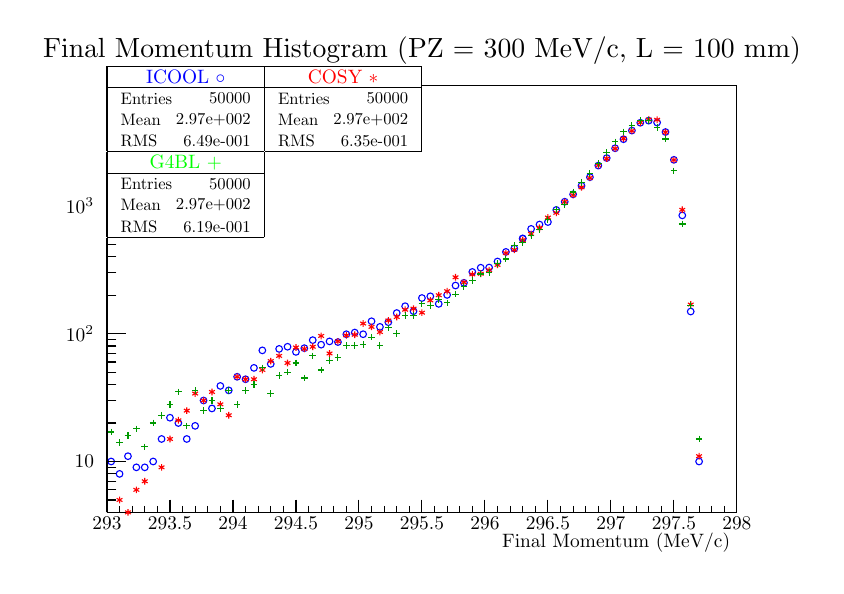
\begin{tikzpicture}
\definecolor{c}{rgb}{1,1,1};
\draw [color=c, fill=c] (0,0) rectangle (20,13.5632);
\draw [color=c, fill=c] (2,1.35632) rectangle (18,12.2069);
\definecolor{c}{rgb}{0,0,0};
\draw [c] (2,1.35632) -- (2,12.2069) -- (18,12.2069) -- (18,1.35632) -- (2,1.35632);
\definecolor{c}{rgb}{1,1,1};
\draw [color=c, fill=c] (2,1.35632) rectangle (18,12.2069);
\definecolor{c}{rgb}{0,0,0};
\draw [c] (2,1.35632) -- (2,12.2069) -- (18,12.2069) -- (18,1.35632) -- (2,1.35632);
\definecolor{c}{rgb}{0,0,1};
\foreach \P in
 {(2.10667,2.64836),(2.32,2.33371),(2.53333,2.78275),(2.74667,2.49979),(2.96,2.49979),(3.17333,2.64836),(3.38667,3.2201),(3.6,3.76014),(3.81333,3.62575),(4.02667,3.2201),(4.24,3.55342),(4.45333,4.19748),(4.66667,3.9957),(4.88,4.56744),(5.09333,4.4545
7),(5.30667,4.80021),(5.52,4.73753),(5.73333,5.02631),(5.94667,5.47059),(6.16,5.12707),(6.37333,5.5082),(6.58667,5.56279),(6.8,5.43196),(7.01333,5.52663),(7.22667,5.73085),(7.44,5.61534),(7.65333,5.6988),(7.86667,5.6825),(8.08,5.881),(8.29333,5.9231)
,(8.50667,5.881),(8.72,6.20982),(8.93333,6.06751),(9.14667,6.18708),(9.36,6.41911),(9.57333,6.59273),(9.78667,6.46691),(10,6.80024),(10.2133,6.84408),(10.4267,6.65167),(10.64,6.8796),(10.8533,7.11785),(11.0667,7.18721),(11.28,7.46298),(11.4933,7.5701
2),(11.7067,7.57441),(11.92,7.72854),(12.1333,7.97147),(12.3467,8.05924),(12.56,8.31176)}{\draw[mark options={color=c,fill=c},mark size=2.402402pt,mark=o] plot coordinates {\P};}
\foreach \P in
 {(12.56,8.31176),(12.7733,8.55608),(12.9867,8.66698),(13.2,8.73069),(13.4133,9.03814),(13.6267,9.24659),(13.84,9.43504),(14.0533,9.65322),(14.2667,9.87017),(14.48,10.1645),(14.6933,10.3552),(14.9067,10.6044),(15.12,10.8336),(15.3333,11.0545),(15.546
7,11.2525),(15.76,11.3057),(15.9733,11.2588),(16.1867,11.017),(16.4,10.3109),(16.6133,8.89949),(16.8267,6.45748),(17.04,2.64836)}{\draw[mark options={color=c,fill=c},mark size=2.402402pt,mark=o] plot coordinates {\P};}
\definecolor{c}{rgb}{1,1,1};
\draw [color=c, fill=c] (2,10.5115) rectangle (6,12.6816);
\definecolor{c}{rgb}{0,0,0};
\draw [c] (2,10.5115) -- (6,10.5115);
\draw [c] (6,10.5115) -- (6,12.6816);
\draw [c] (6,12.6816) -- (2,12.6816);
\draw [c] (2,12.6816) -- (2,10.5115);
\draw[color=blue](4,12.4103) node[scale=0.7, rotate=0]{ICOOL $\circ$};
\draw [c] (2,12.1391) -- (6,12.1391);
\draw [anchor= west] (2.2,11.8678) node[scale=0.6, rotate=0]{Entries };
\draw [anchor= east] (5.8,11.8678) node[scale=0.6, rotate=0]{ 50000};
\draw [anchor= west] (2.2,11.3253) node[scale=0.6, rotate=0]{Mean  };
\draw [anchor= east] (5.8,11.3253) node[scale=0.6, rotate=0]{ 2.97e+002};
\draw [anchor= west] (2.2,10.7828) node[scale=0.6, rotate=0]{RMS   };
\draw [anchor= east] (5.8,10.7828) node[scale=0.6, rotate=0]{ 6.49e-001};
\draw [c] (2,1.35632) -- (18,1.35632);
\draw [anchor= east] (18,0.596782) node[scale=0.7, rotate=0]{Final Momentum (MeV/c)};
\draw [c] (2,1.68184) -- (2,1.35632);
\draw [c] (2.32,1.51908) -- (2.32,1.35632);
\draw [c] (2.64,1.51908) -- (2.64,1.35632);
\draw [c] (2.96,1.51908) -- (2.96,1.35632);
\draw [c] (3.28,1.51908) -- (3.28,1.35632);
\draw [c] (3.6,1.68184) -- (3.6,1.35632);
\draw [c] (3.92,1.51908) -- (3.92,1.35632);
\draw [c] (4.24,1.51908) -- (4.24,1.35632);
\draw [c] (4.56,1.51908) -- (4.56,1.35632);
\draw [c] (4.88,1.51908) -- (4.88,1.35632);
\draw [c] (5.2,1.68184) -- (5.2,1.35632);
\draw [c] (5.52,1.51908) -- (5.52,1.35632);
\draw [c] (5.84,1.51908) -- (5.84,1.35632);
\draw [c] (6.16,1.51908) -- (6.16,1.35632);
\draw [c] (6.48,1.51908) -- (6.48,1.35632);
\draw [c] (6.8,1.68184) -- (6.8,1.35632);
\draw [c] (7.12,1.51908) -- (7.12,1.35632);
\draw [c] (7.44,1.51908) -- (7.44,1.35632);
\draw [c] (7.76,1.51908) -- (7.76,1.35632);
\draw [c] (8.08,1.51908) -- (8.08,1.35632);
\draw [c] (8.4,1.68184) -- (8.4,1.35632);
\draw [c] (8.72,1.51908) -- (8.72,1.35632);
\draw [c] (9.04,1.51908) -- (9.04,1.35632);
\draw [c] (9.36,1.51908) -- (9.36,1.35632);
\draw [c] (9.68,1.51908) -- (9.68,1.35632);
\draw [c] (10,1.68184) -- (10,1.35632);
\draw [c] (10.32,1.51908) -- (10.32,1.35632);
\draw [c] (10.64,1.51908) -- (10.64,1.35632);
\draw [c] (10.96,1.51908) -- (10.96,1.35632);
\draw [c] (11.28,1.51908) -- (11.28,1.35632);
\draw [c] (11.6,1.68184) -- (11.6,1.35632);
\draw [c] (11.92,1.51908) -- (11.92,1.35632);
\draw [c] (12.24,1.51908) -- (12.24,1.35632);
\draw [c] (12.56,1.51908) -- (12.56,1.35632);
\draw [c] (12.88,1.51908) -- (12.88,1.35632);
\draw [c] (13.2,1.68184) -- (13.2,1.35632);
\draw [c] (13.52,1.51908) -- (13.52,1.35632);
\draw [c] (13.84,1.51908) -- (13.84,1.35632);
\draw [c] (14.16,1.51908) -- (14.16,1.35632);
\draw [c] (14.48,1.51908) -- (14.48,1.35632);
\draw [c] (14.8,1.68184) -- (14.8,1.35632);
\draw [c] (15.12,1.51908) -- (15.12,1.35632);
\draw [c] (15.44,1.51908) -- (15.44,1.35632);
\draw [c] (15.76,1.51908) -- (15.76,1.35632);
\draw [c] (16.08,1.51908) -- (16.08,1.35632);
\draw [c] (16.4,1.68184) -- (16.4,1.35632);
\draw [c] (16.72,1.51908) -- (16.72,1.35632);
\draw [c] (17.04,1.51908) -- (17.04,1.35632);
\draw [c] (17.36,1.51908) -- (17.36,1.35632);
\draw [c] (17.68,1.51908) -- (17.68,1.35632);
\draw [c] (18,1.68184) -- (18,1.35632);
\draw [anchor=base] (2,0.908736) node[scale=0.7, rotate=0]{293};
\draw [anchor=base] (3.6,0.908736) node[scale=0.7, rotate=0]{293.5};
\draw [anchor=base] (5.2,0.908736) node[scale=0.7, rotate=0]{294};
\draw [anchor=base] (6.8,0.908736) node[scale=0.7, rotate=0]{294.5};
\draw [anchor=base] (8.4,0.908736) node[scale=0.7, rotate=0]{295};
\draw [anchor=base] (10,0.908736) node[scale=0.7, rotate=0]{295.5};
\draw [anchor=base] (11.6,0.908736) node[scale=0.7, rotate=0]{296};
\draw [anchor=base] (13.2,0.908736) node[scale=0.7, rotate=0]{296.5};
\draw [anchor=base] (14.8,0.908736) node[scale=0.7, rotate=0]{297};
\draw [anchor=base] (16.4,0.908736) node[scale=0.7, rotate=0]{297.5};
\draw [anchor=base] (18,0.908736) node[scale=0.7, rotate=0]{298};
\draw [c] (2,1.35632) -- (2,12.2069);
\draw [c] (2.24,1.67097) -- (2,1.67097);
\draw [c] (2.24,1.92805) -- (2,1.92805);
\draw [c] (2.24,2.14542) -- (2,2.14542);
\draw [c] (2.24,2.33371) -- (2,2.33371);
\draw [c] (2.24,2.49979) -- (2,2.49979);
\draw [c] (2.48,2.64836) -- (2,2.64836);
\draw [anchor= east] (1.844,2.64836) node[scale=0.7, rotate=0]{10};
\draw [c] (2.24,3.62575) -- (2,3.62575);
\draw [c] (2.24,4.19748) -- (2,4.19748);
\draw [c] (2.24,4.60313) -- (2,4.60313);
\draw [c] (2.24,4.91778) -- (2,4.91778);
\draw [c] (2.24,5.17487) -- (2,5.17487);
\draw [c] (2.24,5.39223) -- (2,5.39223);
\draw [c] (2.24,5.58052) -- (2,5.58052);
\draw [c] (2.24,5.74661) -- (2,5.74661);
\draw [c] (2.48,5.89517) -- (2,5.89517);
\draw [anchor= east] (1.844,5.89517) node[scale=0.7, rotate=0]{$10^{2}$};
\draw [c] (2.24,6.87256) -- (2,6.87256);
\draw [c] (2.24,7.4443) -- (2,7.4443);
\draw [c] (2.24,7.84995) -- (2,7.84995);
\draw [c] (2.24,8.1646) -- (2,8.1646);
\draw [c] (2.24,8.42169) -- (2,8.42169);
\draw [c] (2.24,8.63905) -- (2,8.63905);
\draw [c] (2.24,8.82734) -- (2,8.82734);
\draw [c] (2.24,8.99342) -- (2,8.99342);
\draw [c] (2.48,9.14199) -- (2,9.14199);
\draw [anchor= east] (1.844,9.14199) node[scale=0.7, rotate=0]{$10^{3}$};
\draw [c] (2.24,10.1194) -- (2,10.1194);
\draw [c] (2.24,10.6911) -- (2,10.6911);
\draw [c] (2.24,11.0968) -- (2,11.0968);
\draw [c] (2.24,11.4114) -- (2,11.4114);
\draw [c] (2.24,11.6685) -- (2,11.6685);
\draw [c] (2.24,11.8859) -- (2,11.8859);
\draw [c] (2.24,12.0742) -- (2,12.0742);
\definecolor{c}{rgb}{1,1,1};
\draw [color=c, fill=c] (2,10.5115) rectangle (6,12.6816);
\definecolor{c}{rgb}{0,0,0};
\draw [c] (2,10.5115) -- (6,10.5115);
\draw [c] (6,10.5115) -- (6,12.6816);
\draw [c] (6,12.6816) -- (2,12.6816);
\draw [c] (2,12.6816) -- (2,10.5115);
\draw[color=blue](4,12.4103) node[scale=0.7, rotate=0]{ICOOL $\circ$};
\draw [c] (2,12.1391) -- (6,12.1391);
\draw [anchor= west] (2.2,11.8678) node[scale=0.6, rotate=0]{Entries };
\draw [anchor= east] (5.8,11.8678) node[scale=0.6, rotate=0]{ 50000};
\draw [anchor= west] (2.2,11.3253) node[scale=0.6, rotate=0]{Mean  };
\draw [anchor= east] (5.8,11.3253) node[scale=0.6, rotate=0]{ 2.97e+002};
\draw [anchor= west] (2.2,10.7828) node[scale=0.6, rotate=0]{RMS   };
\draw [anchor= east] (5.8,10.7828) node[scale=0.6, rotate=0]{ 6.49e-001};
\draw (10,13.0816) node[scale=1, rotate=0]{Final Momentum Histogram (PZ = 300 MeV/c, L = 100 mm)};
\definecolor{c}{rgb}{1,0,0};
\foreach \P in
 {(2.32,1.67097),(2.53333,1.35632),(2.74667,1.92806),(2.96,2.14542),(3.38667,2.49979),(3.6,3.2201),(3.81333,3.69455),(4.02667,3.9404),(4.24,4.37397),(4.45333,4.19748),(4.66667,4.41485),(4.88,4.1002),(5.09333,3.82282),(5.30667,4.80021),(5.52,4.73753),
(5.73333,4.73753),(5.94667,4.97309),(6.16,5.19818),(6.37333,5.33047),(6.58667,5.15117),(6.8,5.54483),(7.01333,5.5082),(7.22667,5.56279),(7.44,5.83761),(7.65333,5.39224),(7.86667,5.6988),(8.08,5.85222),(8.29333,5.86669),(8.50667,6.15226),(8.72,6.06751
),(8.93333,5.93685),(9.14667,6.23221),(9.36,6.31834),(9.57333,6.50402),(9.78667,6.53122),(10,6.4288),(10.2133,6.73958),(10.4267,6.87256),(10.64,6.97454),(10.8533,7.32673),(11.0667,7.19845),(11.28,7.40135),(11.4933,7.41581),(11.7067,7.50861),(11.92,7.
64137),(12.1333,7.94206),(12.3467,8.0254),(12.56,8.27312),(12.7733,8.42872),(12.9867,8.57729)}{\draw[mark options={color=c,fill=c},mark size=2.402402pt,mark=asterisk] plot coordinates {\P};}
\foreach \P in
 {(12.9867,8.57729),(13.2,8.84486),(13.4133,8.96334),(13.6267,9.24265),(13.84,9.41427),(14.0533,9.61139),(14.2667,9.85153),(14.48,10.172),(14.6933,10.3408),(14.9067,10.5968),(15.12,10.8484),(15.3333,11.0458),(15.5467,11.2585),(15.76,11.3325),(15.9733
,11.3284),(16.1867,11.0118),(16.4,10.3054),(16.6133,9.04117),(16.8267,6.63508),(17.04,2.78275)}{\draw[mark options={color=c,fill=c},mark size=2.402402pt,mark=asterisk] plot coordinates {\P};}
\definecolor{c}{rgb}{1,1,1};
\draw [color=c, fill=c] (6,10.5115) rectangle (10,12.6816);
\definecolor{c}{rgb}{0,0,0};
\draw [c] (6,10.5115) -- (10,10.5115);
\draw [c] (10,10.5115) -- (10,12.6816);
\draw [c] (10,12.6816) -- (6,12.6816);
\draw [c] (6,12.6816) -- (6,10.5115);
\draw [color=red](8,12.4103) node[scale=0.7, rotate=0]{COSY $*$};
\draw [c] (6,12.1391) -- (10,12.1391);
\draw [anchor= west] (6.2,11.8678) node[scale=0.6, rotate=0]{Entries };
\draw [anchor= east] (9.8,11.8678) node[scale=0.6, rotate=0]{ 50000};
\draw [anchor= west] (6.2,11.3253) node[scale=0.6, rotate=0]{Mean  };
\draw [anchor= east] (9.8,11.3253) node[scale=0.6, rotate=0]{ 2.97e+002};
\draw [anchor= west] (6.2,10.7828) node[scale=0.6, rotate=0]{RMS   };
\draw [anchor= east] (9.8,10.7828) node[scale=0.6, rotate=0]{ 6.35e-001};
\definecolor{c}{rgb}{1,1,1};
\draw [color=c, fill=c] (6,10.5115) rectangle (10,12.6816);
\definecolor{c}{rgb}{0,0,0};
\draw [c] (6,10.5115) -- (10,10.5115);
\draw [c] (10,10.5115) -- (10,12.6816);
\draw [c] (10,12.6816) -- (6,12.6816);
\draw [c] (6,12.6816) -- (6,10.5115);
\draw [color=red](8,12.4103) node[scale=0.7, rotate=0]{COSY $*$};
\draw [c] (6,12.1391) -- (10,12.1391);
\draw [anchor= west] (6.2,11.8678) node[scale=0.6, rotate=0]{Entries };
\draw [anchor= east] (9.8,11.8678) node[scale=0.6, rotate=0]{ 50000};
\draw [anchor= west] (6.2,11.3253) node[scale=0.6, rotate=0]{Mean  };
\draw [anchor= east] (9.8,11.3253) node[scale=0.6, rotate=0]{ 2.97e+002};
\draw [anchor= west] (6.2,10.7828) node[scale=0.6, rotate=0]{RMS   };
\draw [anchor= east] (9.8,10.7828) node[scale=0.6, rotate=0]{ 6.35e-001};
\definecolor{c}{rgb}{0,0.6,0};
\foreach \P in
 {(2.10667,3.39658),(2.32,3.12281),(2.53333,3.3111),(2.74667,3.47718),(2.96,3.01831),(3.17333,3.62575),(3.38667,3.82282),(3.6,4.1002),(3.81333,4.41485),(4.02667,3.55342),(4.24,4.45457),(4.45333,3.9404),(4.66667,4.19748),(4.88,3.9957),(5.09333,4.45457
),(5.30667,4.1002),(5.52,4.45457),(5.73333,4.60314),(5.94667,5.02631),(6.16,4.37397),(6.37333,4.83054),(6.58667,4.91779),(6.8,5.15117),(7.01333,4.76922),(7.22667,5.33047),(7.44,4.97309),(7.65333,5.22111),(7.86667,5.28774),(8.08,5.59804),(8.29333,5.59
804),(8.50667,5.61534),(8.72,5.80793),(8.93333,5.59804),(9.14667,6.04233),(9.36,5.89517),(9.57333,6.34934),(9.78667,6.34934),(10,6.65167),(10.2133,6.60982),(10.4267,6.77023),(10.64,6.67619),(10.8533,6.90049),(11.0667,7.08791),(11.28,7.24252),(11.4933
,7.41101),(11.7067,7.44899),(11.92,7.68166),(12.1333,7.79239),(12.3467,8.13323),(12.56,8.21175)}{\draw[mark options={color=c,fill=c},mark size=2.402402pt,mark=+] plot coordinates {\P};}
\foreach \P in
 {(12.56,8.21175),(12.7733,8.3908),(12.9867,8.53455),(13.2,8.79164),(13.4133,9.05624),(13.6267,9.17681),(13.84,9.49338),(14.0533,9.74165),(14.2667,9.96217),(14.48,10.2095),(14.6933,10.4947),(14.9067,10.7666),(15.12,11.0189),(15.3333,11.1816),(15.5467
,11.3045),(15.76,11.3036),(15.9733,11.1288),(16.1867,10.84),(16.4,10.0299),(16.6133,8.68073),(16.8267,6.60982),(17.04,3.2201)}{\draw[mark options={color=c,fill=c},mark size=2.402402pt,mark=+] plot coordinates {\P};}
\definecolor{c}{rgb}{1,1,1};
\draw [color=c, fill=c] (2,8.34138) rectangle (6,10.5115);
\definecolor{c}{rgb}{0,0,0};
\draw [c] (2,8.34138) -- (6,8.34138);
\draw [c] (6,8.34138) -- (6,10.5115);
\draw [c] (6,10.5115) -- (2,10.5115);
\draw [c] (2,10.5115) -- (2,8.34138);
\draw [color=green](4,10.2402) node[scale=0.7, rotate=0]{G4BL $+$};
\draw [c] (2,9.96897) -- (6,9.96897);
\draw [anchor= west] (2.2,9.6977) node[scale=0.6, rotate=0]{Entries };
\draw [anchor= east] (5.8,9.6977) node[scale=0.6, rotate=0]{ 50000};
\draw [anchor= west] (2.2,9.15517) node[scale=0.6, rotate=0]{Mean  };
\draw [anchor= east] (5.8,9.15517) node[scale=0.6, rotate=0]{ 2.97e+002};
\draw [anchor= west] (2.2,8.61264) node[scale=0.6, rotate=0]{RMS   };
\draw [anchor= east] (5.8,8.61264) node[scale=0.6, rotate=0]{ 6.19e-001};
\definecolor{c}{rgb}{1,1,1};
\draw [color=c, fill=c] (2,8.34138) rectangle (6,10.5115);
\definecolor{c}{rgb}{0,0,0};
\draw [c] (2,8.34138) -- (6,8.34138);
\draw [c] (6,8.34138) -- (6,10.5115);
\draw [c] (6,10.5115) -- (2,10.5115);
\draw [c] (2,10.5115) -- (2,8.34138);
\draw [color=green](4,10.2402) node[scale=0.7, rotate=0]{G4BL $+$};
\draw [c] (2,9.96897) -- (6,9.96897);
\draw [anchor= west] (2.2,9.6977) node[scale=0.6, rotate=0]{Entries };
\draw [anchor= east] (5.8,9.6977) node[scale=0.6, rotate=0]{ 50000};
\draw [anchor= west] (2.2,9.15517) node[scale=0.6, rotate=0]{Mean  };
\draw [anchor= east] (5.8,9.15517) node[scale=0.6, rotate=0]{ 2.97e+002};
\draw [anchor= west] (2.2,8.61264) node[scale=0.6, rotate=0]{RMS   };
\draw [anchor= east] (5.8,8.61264) node[scale=0.6, rotate=0]{ 6.19e-001};
\end{tikzpicture}
}\\
\frame{      \pgfdeclareplotmark{cross} {
\pgfpathmoveto{\pgfpoint{-0.3\pgfplotmarksize}{\pgfplotmarksize}}
\pgfpathlineto{\pgfpoint{+0.3\pgfplotmarksize}{\pgfplotmarksize}}
\pgfpathlineto{\pgfpoint{+0.3\pgfplotmarksize}{0.3\pgfplotmarksize}}
\pgfpathlineto{\pgfpoint{+1\pgfplotmarksize}{0.3\pgfplotmarksize}}
\pgfpathlineto{\pgfpoint{+1\pgfplotmarksize}{-0.3\pgfplotmarksize}}
\pgfpathlineto{\pgfpoint{+0.3\pgfplotmarksize}{-0.3\pgfplotmarksize}}
\pgfpathlineto{\pgfpoint{+0.3\pgfplotmarksize}{-1.\pgfplotmarksize}}
\pgfpathlineto{\pgfpoint{-0.3\pgfplotmarksize}{-1.\pgfplotmarksize}}
\pgfpathlineto{\pgfpoint{-0.3\pgfplotmarksize}{-0.3\pgfplotmarksize}}
\pgfpathlineto{\pgfpoint{-1.\pgfplotmarksize}{-0.3\pgfplotmarksize}}
\pgfpathlineto{\pgfpoint{-1.\pgfplotmarksize}{0.3\pgfplotmarksize}}
\pgfpathlineto{\pgfpoint{-0.3\pgfplotmarksize}{0.3\pgfplotmarksize}}
\pgfpathclose
\pgfusepathqstroke
}
\pgfdeclareplotmark{cross*} {
\pgfpathmoveto{\pgfpoint{-0.3\pgfplotmarksize}{\pgfplotmarksize}}
\pgfpathlineto{\pgfpoint{+0.3\pgfplotmarksize}{\pgfplotmarksize}}
\pgfpathlineto{\pgfpoint{+0.3\pgfplotmarksize}{0.3\pgfplotmarksize}}
\pgfpathlineto{\pgfpoint{+1\pgfplotmarksize}{0.3\pgfplotmarksize}}
\pgfpathlineto{\pgfpoint{+1\pgfplotmarksize}{-0.3\pgfplotmarksize}}
\pgfpathlineto{\pgfpoint{+0.3\pgfplotmarksize}{-0.3\pgfplotmarksize}}
\pgfpathlineto{\pgfpoint{+0.3\pgfplotmarksize}{-1.\pgfplotmarksize}}
\pgfpathlineto{\pgfpoint{-0.3\pgfplotmarksize}{-1.\pgfplotmarksize}}
\pgfpathlineto{\pgfpoint{-0.3\pgfplotmarksize}{-0.3\pgfplotmarksize}}
\pgfpathlineto{\pgfpoint{-1.\pgfplotmarksize}{-0.3\pgfplotmarksize}}
\pgfpathlineto{\pgfpoint{-1.\pgfplotmarksize}{0.3\pgfplotmarksize}}
\pgfpathlineto{\pgfpoint{-0.3\pgfplotmarksize}{0.3\pgfplotmarksize}}
\pgfpathclose
\pgfusepathqfillstroke
}
\pgfdeclareplotmark{newstar} {
\pgfpathmoveto{\pgfqpoint{0pt}{\pgfplotmarksize}}
\pgfpathlineto{\pgfqpointpolar{44}{0.5\pgfplotmarksize}}
\pgfpathlineto{\pgfqpointpolar{18}{\pgfplotmarksize}}
\pgfpathlineto{\pgfqpointpolar{-20}{0.5\pgfplotmarksize}}
\pgfpathlineto{\pgfqpointpolar{-54}{\pgfplotmarksize}}
\pgfpathlineto{\pgfqpointpolar{-90}{0.5\pgfplotmarksize}}
\pgfpathlineto{\pgfqpointpolar{234}{\pgfplotmarksize}}
\pgfpathlineto{\pgfqpointpolar{198}{0.5\pgfplotmarksize}}
\pgfpathlineto{\pgfqpointpolar{162}{\pgfplotmarksize}}
\pgfpathlineto{\pgfqpointpolar{134}{0.5\pgfplotmarksize}}
\pgfpathclose
\pgfusepathqstroke
}
\pgfdeclareplotmark{newstar*} {
\pgfpathmoveto{\pgfqpoint{0pt}{\pgfplotmarksize}}
\pgfpathlineto{\pgfqpointpolar{44}{0.5\pgfplotmarksize}}
\pgfpathlineto{\pgfqpointpolar{18}{\pgfplotmarksize}}
\pgfpathlineto{\pgfqpointpolar{-20}{0.5\pgfplotmarksize}}
\pgfpathlineto{\pgfqpointpolar{-54}{\pgfplotmarksize}}
\pgfpathlineto{\pgfqpointpolar{-90}{0.5\pgfplotmarksize}}
\pgfpathlineto{\pgfqpointpolar{234}{\pgfplotmarksize}}
\pgfpathlineto{\pgfqpointpolar{198}{0.5\pgfplotmarksize}}
\pgfpathlineto{\pgfqpointpolar{162}{\pgfplotmarksize}}
\pgfpathlineto{\pgfqpointpolar{134}{0.5\pgfplotmarksize}}
\pgfpathclose
\pgfusepathqfillstroke
}
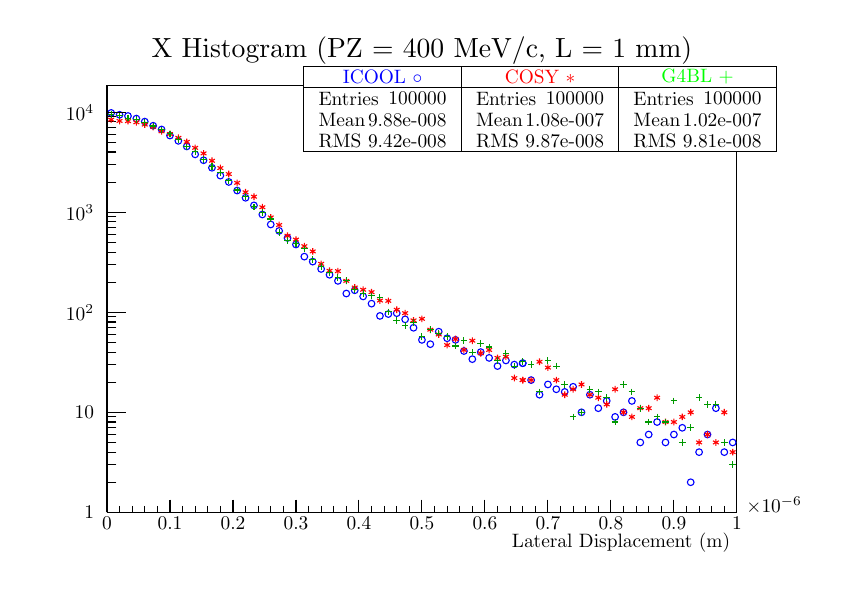
\begin{tikzpicture}
\definecolor{c}{rgb}{1,1,1};
\draw [color=c, fill=c] (0,0) rectangle (20,13.5632);
\draw [color=c, fill=c] (2,1.35632) rectangle (18,12.2069);
\definecolor{c}{rgb}{0,0,0};
\draw [c] (2,1.35632) -- (2,12.2069) -- (18,12.2069) -- (18,1.35632) -- (2,1.35632);
\definecolor{c}{rgb}{1,1,1};
\draw [color=c, fill=c] (2,1.35632) rectangle (18,12.2069);
\definecolor{c}{rgb}{0,0,0};
\draw [c] (2,1.35632) -- (2,12.2069) -- (18,12.2069) -- (18,1.35632) -- (2,1.35632);
\definecolor{c}{rgb}{0,0,1};
\foreach \P in
 {(2.10667,11.5017),(2.32,11.4549),(2.53333,11.4241),(2.74667,11.3581),(2.96,11.2811),(3.17333,11.1766),(3.38667,11.0813),(3.6,10.9273),(3.81333,10.7928),(4.02667,10.6507),(4.24,10.449),(4.45333,10.2999),(4.66667,10.1089),(4.88,9.90959),(5.09333,9.74
886),(5.30667,9.53029),(5.52,9.34637),(5.73333,9.15322),(5.94667,8.92242),(6.16,8.6689),(6.37333,8.50535),(6.58667,8.32531),(6.8,8.15985),(7.01333,7.85163),(7.22667,7.7251),(7.44,7.53825),(7.65333,7.39032),(7.86667,7.23563),(8.08,6.91459),(8.29333,6.
99739),(8.50667,6.8405),(8.72,6.65755),(8.93333,6.34611),(9.14667,6.39307),(9.36,6.41583),(9.57333,6.25878),(9.78667,6.04453),(10,5.73753),(10.2133,5.62819),(10.4267,5.94564),(10.64,5.77841),(10.8533,5.73753),(11.0667,5.45424),(11.28,5.24766),(11.493
3,5.427),(11.7067,5.27964),(11.92,5.07213),(12.1333,5.21471),(12.3467,5.10954),(12.56,5.14572)}{\draw[mark options={color=c,fill=c},mark size=2.402402pt,mark=o] plot coordinates {\P};}
\foreach \P in
 {(12.56,5.14572),(12.7733,4.71595),(12.9867,4.34465),(13.2,4.60551),(13.4133,4.48277),(13.6267,4.41587),(13.84,4.54584),(14.0533,3.89722),(14.2667,4.34465),(14.48,4.0024),(14.6933,4.18674),(14.9067,3.78096),(15.12,3.89722),(15.3333,4.18674),(15.5467
,3.13233),(15.76,3.33353),(15.9733,3.65098),(16.1867,3.13233),(16.4,3.33353),(16.6133,3.50363),(16.8267,2.12121),(17.04,2.8861),(17.2533,3.33353),(17.4667,4.0024),(17.68,2.8861),(17.8933,3.13233)}{\draw[mark options={color=c,fill=c},mark
 size=2.402402pt,mark=o] plot coordinates {\P};}
\definecolor{c}{rgb}{1,1,1};
\draw [color=c, fill=c] (7,10.5115) rectangle (11,12.6816);
\definecolor{c}{rgb}{0,0,0};
\draw [c] (7,10.5115) -- (11,10.5115);
\draw [c] (11,10.5115) -- (11,12.6816);
\draw [c] (11,12.6816) -- (7,12.6816);
\draw [c] (7,12.6816) -- (7,10.5115);
\draw[color=blue](9,12.4103) node[scale=0.7, rotate=0]{ICOOL $\circ$};
\draw [c] (7,12.1391) -- (11,12.1391);
\draw [anchor= west] (7.2,11.8678) node[scale=0.7, rotate=0]{Entries };
\draw [anchor= east] (10.8,11.8678) node[scale=0.7, rotate=0]{ 100000};
\draw [anchor= west] (7.2,11.3253) node[scale=0.7, rotate=0]{Mean  };
\draw [anchor= east] (10.8,11.3253) node[scale=0.7, rotate=0]{ 9.88e-008};
\draw [anchor= west] (7.2,10.7828) node[scale=0.7, rotate=0]{RMS   };
\draw [anchor= east] (10.8,10.7828) node[scale=0.7, rotate=0]{ 9.42e-008};
\draw [c] (2,1.35632) -- (18,1.35632);
\draw [anchor= east] (18,0.596782) node[scale=0.7, rotate=0]{Lateral Displacement (m)};
\draw [c] (2,1.68184) -- (2,1.35632);
\draw [c] (2.32,1.51908) -- (2.32,1.35632);
\draw [c] (2.64,1.51908) -- (2.64,1.35632);
\draw [c] (2.96,1.51908) -- (2.96,1.35632);
\draw [c] (3.28,1.51908) -- (3.28,1.35632);
\draw [c] (3.6,1.68184) -- (3.6,1.35632);
\draw [c] (3.92,1.51908) -- (3.92,1.35632);
\draw [c] (4.24,1.51908) -- (4.24,1.35632);
\draw [c] (4.56,1.51908) -- (4.56,1.35632);
\draw [c] (4.88,1.51908) -- (4.88,1.35632);
\draw [c] (5.2,1.68184) -- (5.2,1.35632);
\draw [c] (5.52,1.51908) -- (5.52,1.35632);
\draw [c] (5.84,1.51908) -- (5.84,1.35632);
\draw [c] (6.16,1.51908) -- (6.16,1.35632);
\draw [c] (6.48,1.51908) -- (6.48,1.35632);
\draw [c] (6.8,1.68184) -- (6.8,1.35632);
\draw [c] (7.12,1.51908) -- (7.12,1.35632);
\draw [c] (7.44,1.51908) -- (7.44,1.35632);
\draw [c] (7.76,1.51908) -- (7.76,1.35632);
\draw [c] (8.08,1.51908) -- (8.08,1.35632);
\draw [c] (8.4,1.68184) -- (8.4,1.35632);
\draw [c] (8.72,1.51908) -- (8.72,1.35632);
\draw [c] (9.04,1.51908) -- (9.04,1.35632);
\draw [c] (9.36,1.51908) -- (9.36,1.35632);
\draw [c] (9.68,1.51908) -- (9.68,1.35632);
\draw [c] (10,1.68184) -- (10,1.35632);
\draw [c] (10.32,1.51908) -- (10.32,1.35632);
\draw [c] (10.64,1.51908) -- (10.64,1.35632);
\draw [c] (10.96,1.51908) -- (10.96,1.35632);
\draw [c] (11.28,1.51908) -- (11.28,1.35632);
\draw [c] (11.6,1.68184) -- (11.6,1.35632);
\draw [c] (11.92,1.51908) -- (11.92,1.35632);
\draw [c] (12.24,1.51908) -- (12.24,1.35632);
\draw [c] (12.56,1.51908) -- (12.56,1.35632);
\draw [c] (12.88,1.51908) -- (12.88,1.35632);
\draw [c] (13.2,1.68184) -- (13.2,1.35632);
\draw [c] (13.52,1.51908) -- (13.52,1.35632);
\draw [c] (13.84,1.51908) -- (13.84,1.35632);
\draw [c] (14.16,1.51908) -- (14.16,1.35632);
\draw [c] (14.48,1.51908) -- (14.48,1.35632);
\draw [c] (14.8,1.68184) -- (14.8,1.35632);
\draw [c] (15.12,1.51908) -- (15.12,1.35632);
\draw [c] (15.44,1.51908) -- (15.44,1.35632);
\draw [c] (15.76,1.51908) -- (15.76,1.35632);
\draw [c] (16.08,1.51908) -- (16.08,1.35632);
\draw [c] (16.4,1.68184) -- (16.4,1.35632);
\draw [c] (16.72,1.51908) -- (16.72,1.35632);
\draw [c] (17.04,1.51908) -- (17.04,1.35632);
\draw [c] (17.36,1.51908) -- (17.36,1.35632);
\draw [c] (17.68,1.51908) -- (17.68,1.35632);
\draw [c] (18,1.68184) -- (18,1.35632);
\draw [c] (18,1.68184) -- (18,1.35632);
\draw [anchor=base] (2,0.908736) node[scale=0.7, rotate=0]{0};
\draw [anchor=base] (3.6,0.908736) node[scale=0.7, rotate=0]{0.1};
\draw [anchor=base] (5.2,0.908736) node[scale=0.7, rotate=0]{0.2};
\draw [anchor=base] (6.8,0.908736) node[scale=0.7, rotate=0]{0.3};
\draw [anchor=base] (8.4,0.908736) node[scale=0.7, rotate=0]{0.4};
\draw [anchor=base] (10,0.908736) node[scale=0.7, rotate=0]{0.5};
\draw [anchor=base] (11.6,0.908736) node[scale=0.7, rotate=0]{0.6};
\draw [anchor=base] (13.2,0.908736) node[scale=0.7, rotate=0]{0.7};
\draw [anchor=base] (14.8,0.908736) node[scale=0.7, rotate=0]{0.8};
\draw [anchor=base] (16.4,0.908736) node[scale=0.7, rotate=0]{0.9};
\draw [anchor=base] (18,0.908736) node[scale=0.7, rotate=0]{1};
\draw [anchor=base west] (18.07,1.35632) node[scale=0.7, rotate=0]{$\times10^{-6}$};
\draw [c] (2,1.35632) -- (2,12.2069);
\draw [c] (2.48,1.35632) -- (2,1.35632);
\draw [anchor= east] (1.844,1.35632) node[scale=0.7, rotate=0]{1};
\draw [c] (2.24,2.12121) -- (2,2.12121);
\draw [c] (2.24,2.56864) -- (2,2.56864);
\draw [c] (2.24,2.8861) -- (2,2.8861);
\draw [c] (2.24,3.13234) -- (2,3.13234);
\draw [c] (2.24,3.33353) -- (2,3.33353);
\draw [c] (2.24,3.50363) -- (2,3.50363);
\draw [c] (2.24,3.65098) -- (2,3.65098);
\draw [c] (2.24,3.78096) -- (2,3.78096);
\draw [c] (2.48,3.89722) -- (2,3.89722);
\draw [anchor= east] (1.844,3.89722) node[scale=0.7, rotate=0]{10};
\draw [c] (2.24,4.66211) -- (2,4.66211);
\draw [c] (2.24,5.10954) -- (2,5.10954);
\draw [c] (2.24,5.427) -- (2,5.427);
\draw [c] (2.24,5.67324) -- (2,5.67324);
\draw [c] (2.24,5.87443) -- (2,5.87443);
\draw [c] (2.24,6.04453) -- (2,6.04453);
\draw [c] (2.24,6.19188) -- (2,6.19188);
\draw [c] (2.24,6.32186) -- (2,6.32186);
\draw [c] (2.48,6.43812) -- (2,6.43812);
\draw [anchor= east] (1.844,6.43812) node[scale=0.7, rotate=0]{$10^{2}$};
\draw [c] (2.24,7.20301) -- (2,7.20301);
\draw [c] (2.24,7.65044) -- (2,7.65044);
\draw [c] (2.24,7.9679) -- (2,7.9679);
\draw [c] (2.24,8.21413) -- (2,8.21413);
\draw [c] (2.24,8.41533) -- (2,8.41533);
\draw [c] (2.24,8.58543) -- (2,8.58543);
\draw [c] (2.24,8.73278) -- (2,8.73278);
\draw [c] (2.24,8.86276) -- (2,8.86276);
\draw [c] (2.48,8.97902) -- (2,8.97902);
\draw [anchor= east] (1.844,8.97902) node[scale=0.7, rotate=0]{$10^{3}$};
\draw [c] (2.24,9.74391) -- (2,9.74391);
\draw [c] (2.24,10.1913) -- (2,10.1913);
\draw [c] (2.24,10.5088) -- (2,10.5088);
\draw [c] (2.24,10.755) -- (2,10.755);
\draw [c] (2.24,10.9562) -- (2,10.9562);
\draw [c] (2.24,11.1263) -- (2,11.1263);
\draw [c] (2.24,11.2737) -- (2,11.2737);
\draw [c] (2.24,11.4037) -- (2,11.4037);
\draw [c] (2.48,11.5199) -- (2,11.5199);
\draw [anchor= east] (1.844,11.5199) node[scale=0.7, rotate=0]{$10^{4}$};
\definecolor{c}{rgb}{1,1,1};
\draw [color=c, fill=c] (7,10.5115) rectangle (11,12.6816);
\definecolor{c}{rgb}{0,0,0};
\draw [c] (7,10.5115) -- (11,10.5115);
\draw [c] (11,10.5115) -- (11,12.6816);
\draw [c] (11,12.6816) -- (7,12.6816);
\draw [c] (7,12.6816) -- (7,10.5115);
\draw[color=blue](9,12.4103) node[scale=0.7, rotate=0]{ICOOL $\circ$};
\draw [c] (7,12.1391) -- (11,12.1391);
\draw [anchor= west] (7.2,11.8678) node[scale=0.7, rotate=0]{Entries };
\draw [anchor= east] (10.8,11.8678) node[scale=0.7, rotate=0]{ 100000};
\draw [anchor= west] (7.2,11.3253) node[scale=0.7, rotate=0]{Mean  };
\draw [anchor= east] (10.8,11.3253) node[scale=0.7, rotate=0]{ 9.88e-008};
\draw [anchor= west] (7.2,10.7828) node[scale=0.7, rotate=0]{RMS   };
\draw [anchor= east] (10.8,10.7828) node[scale=0.7, rotate=0]{ 9.42e-008};
\draw (10,13.0816) node[scale=1, rotate=0]{X Histogram (PZ = 400 MeV/c, L = 1 mm)};
\definecolor{c}{rgb}{1,0,0};
\foreach \P in
 {(2.10667,11.3309),(2.32,11.2981),(2.53333,11.2935),(2.74667,11.264),(2.96,11.2057),(3.17333,11.1459),(3.38667,11.0338),(3.6,10.9663),(3.81333,10.8696),(4.02667,10.7664),(4.24,10.6145),(4.45333,10.474),(4.66667,10.2861),(4.88,10.1013),(5.09333,9.949
23),(5.30667,9.72499),(5.52,9.48588),(5.73333,9.37449),(5.94667,9.10605),(6.16,8.84794),(6.37333,8.65566),(6.58667,8.38171),(6.8,8.28466),(7.01333,8.11731),(7.22667,7.98432),(7.44,7.66868),(7.65333,7.49253),(7.86667,7.484),(8.08,7.23563),(8.29333,7.0
682),(8.50667,7.01061),(8.72,6.94985),(8.93333,6.7361),(9.14667,6.72764),(9.36,6.50242),(9.57333,6.41583),(9.78667,6.23251),(10,6.27169),(10.2133,5.99619),(10.4267,5.87443),(10.64,5.60495),(10.8533,5.75816),(11.0667,5.48083),(11.28,5.71651),(11.4933,
5.39906),(11.7067,5.48083),(11.92,5.27964),(12.1333,5.31073),(12.3467,4.76728),(12.56,4.71595)}{\draw[mark options={color=c,fill=c},mark size=2.402402pt,mark=asterisk] plot coordinates {\P};}
\foreach \P in
 {(12.56,4.71595),(12.7733,4.71595),(12.9867,5.18076),(13.2,5.0334),(13.4133,4.71595),(13.6267,4.34465),(13.84,4.48277),(14.0533,4.60551),(14.2667,4.34465),(14.48,4.26852),(14.6933,4.09841),(14.9067,4.48277),(15.12,3.89722),(15.3333,3.78096),(15.5467
,4.0024),(15.76,4.0024),(15.9733,4.26852),(16.1867,3.65098),(16.4,3.65098),(16.6133,3.78096),(16.8267,3.89722),(17.04,3.13233),(17.2533,3.33353),(17.4667,3.13233),(17.68,3.89722),(17.8933,2.8861)}{\draw[mark options={color=c,fill=c},mark
 size=2.402402pt,mark=asterisk] plot coordinates {\P};}
\definecolor{c}{rgb}{1,1,1};
\draw [color=c, fill=c] (11,10.5115) rectangle (15,12.6816);
\definecolor{c}{rgb}{0,0,0};
\draw [c] (11,10.5115) -- (15,10.5115);
\draw [c] (15,10.5115) -- (15,12.6816);
\draw [c] (15,12.6816) -- (11,12.6816);
\draw [c] (11,12.6816) -- (11,10.5115);
\draw [color=red](13,12.4103) node[scale=0.7, rotate=0]{COSY $*$};
\draw [c] (11,12.1391) -- (15,12.1391);
\draw [anchor= west] (11.2,11.8678) node[scale=0.7, rotate=0]{Entries };
\draw [anchor= east] (14.8,11.8678) node[scale=0.7, rotate=0]{ 100000};
\draw [anchor= west] (11.2,11.3253) node[scale=0.7, rotate=0]{Mean  };
\draw [anchor= east] (14.8,11.3253) node[scale=0.7, rotate=0]{ 1.08e-007};
\draw [anchor= west] (11.2,10.7828) node[scale=0.7, rotate=0]{RMS   };
\draw [anchor= east] (14.8,10.7828) node[scale=0.7, rotate=0]{ 9.87e-008};
\definecolor{c}{rgb}{1,1,1};
\draw [color=c, fill=c] (11,10.5115) rectangle (15,12.6816);
\definecolor{c}{rgb}{0,0,0};
\draw [c] (11,10.5115) -- (15,10.5115);
\draw [c] (15,10.5115) -- (15,12.6816);
\draw [c] (15,12.6816) -- (11,12.6816);
\draw [c] (11,12.6816) -- (11,10.5115);
\draw [color=red](13,12.4103) node[scale=0.7, rotate=0]{COSY $*$};
\draw [c] (11,12.1391) -- (15,12.1391);
\draw [anchor= west] (11.2,11.8678) node[scale=0.7, rotate=0]{Entries };
\draw [anchor= east] (14.8,11.8678) node[scale=0.7, rotate=0]{ 100000};
\draw [anchor= west] (11.2,11.3253) node[scale=0.7, rotate=0]{Mean  };
\draw [anchor= east] (14.8,11.3253) node[scale=0.7, rotate=0]{ 1.08e-007};
\draw [anchor= west] (11.2,10.7828) node[scale=0.7, rotate=0]{RMS   };
\draw [anchor= east] (14.8,10.7828) node[scale=0.7, rotate=0]{ 9.87e-008};
\definecolor{c}{rgb}{0,0.6,0};
\foreach \P in
 {(2.10667,11.4667),(2.32,11.4265),(2.53333,11.3703),(2.74667,11.3347),(2.96,11.2504),(3.17333,11.1695),(3.38667,11.0702),(3.6,10.9705),(3.81333,10.8303),(4.02667,10.6385),(4.24,10.5173),(4.45333,10.318),(4.66667,10.1374),(4.88,9.98351),(5.09333,9.77
492),(5.30667,9.54426),(5.52,9.38675),(5.73333,9.11389),(5.94667,8.97792),(6.16,8.80873),(6.37333,8.46566),(6.58667,8.26587),(6.8,8.18279),(7.01333,8.0477),(7.22667,7.77878),(7.44,7.5977),(7.65333,7.45365),(7.86667,7.32313),(8.08,7.24097),(8.29333,7.
02367),(8.50667,6.92173),(8.72,6.85572),(8.93333,6.80942),(9.14667,6.4491),(9.36,6.23251),(9.57333,6.10585),(9.78667,6.178),(10,5.81782),(10.2133,5.99619),(10.4267,5.91061),(10.64,5.81782),(10.8533,5.58122),(11.0667,5.71651),(11.28,5.427),(11.4933,5.
65094),(11.7067,5.55697),(11.92,5.21471),(12.1333,5.39906),(12.3467,5.07213),(12.56,5.18076)}{\draw[mark options={color=c,fill=c},mark size=2.402402pt,mark=+] plot coordinates {\P};}
\foreach \P in
 {(12.56,5.18076),(12.7733,5.10954),(12.9867,4.41587),(13.2,5.21471),(13.4133,5.07213),(13.6267,4.60551),(13.84,3.78096),(14.0533,3.89722),(14.2667,4.48277),(14.48,4.41587),(14.6933,4.26852),(14.9067,3.65098),(15.12,4.60551),(15.3333,4.41587),(15.546
7,4.0024),(15.76,3.65098),(15.9733,3.78096),(16.1867,3.65098),(16.4,4.18674),(16.6133,3.13233),(16.8267,3.50363),(17.04,4.26852),(17.2533,4.09841),(17.4667,4.09841),(17.68,3.13233),(17.8933,2.56864)}{\draw[mark options={color=c,fill=c},mark
 size=2.402402pt,mark=+] plot coordinates {\P};}
\definecolor{c}{rgb}{1,1,1};
\draw [color=c, fill=c] (15,10.5115) rectangle (19,12.6816);
\definecolor{c}{rgb}{0,0,0};
\draw [c] (15,10.5115) -- (19,10.5115);
\draw [c] (19,10.5115) -- (19,12.6816);
\draw [c] (19,12.6816) -- (15,12.6816);
\draw [c] (15,12.6816) -- (15,10.5115);
\draw [color=green](17,12.4103) node[scale=0.7, rotate=0]{G4BL $+$};
\draw [c] (15,12.1391) -- (19,12.1391);
\draw [anchor= west] (15.2,11.8678) node[scale=0.7, rotate=0]{Entries };
\draw [anchor= east] (18.8,11.8678) node[scale=0.7, rotate=0]{ 100000};
\draw [anchor= west] (15.2,11.3253) node[scale=0.7, rotate=0]{Mean  };
\draw [anchor= east] (18.8,11.3253) node[scale=0.7, rotate=0]{ 1.02e-007};
\draw [anchor= west] (15.2,10.7828) node[scale=0.7, rotate=0]{RMS   };
\draw [anchor= east] (18.8,10.7828) node[scale=0.7, rotate=0]{ 9.81e-008};
\definecolor{c}{rgb}{1,1,1};
\draw [color=c, fill=c] (15,10.5115) rectangle (19,12.6816);
\definecolor{c}{rgb}{0,0,0};
\draw [c] (15,10.5115) -- (19,10.5115);
\draw [c] (19,10.5115) -- (19,12.6816);
\draw [c] (19,12.6816) -- (15,12.6816);
\draw [c] (15,12.6816) -- (15,10.5115);
\draw [color=green](17,12.4103) node[scale=0.7, rotate=0]{G4BL $+$};
\draw [c] (15,12.1391) -- (19,12.1391);
\draw [anchor= west] (15.2,11.8678) node[scale=0.7, rotate=0]{Entries };
\draw [anchor= east] (18.8,11.8678) node[scale=0.7, rotate=0]{ 100000};
\draw [anchor= west] (15.2,11.3253) node[scale=0.7, rotate=0]{Mean  };
\draw [anchor= east] (18.8,11.3253) node[scale=0.7, rotate=0]{ 1.02e-007};
\draw [anchor= west] (15.2,10.7828) node[scale=0.7, rotate=0]{RMS   };
\draw [anchor= east] (18.8,10.7828) node[scale=0.7, rotate=0]{ 9.81e-008};
\end{tikzpicture}
}\\
\frame{    \pgfdeclareplotmark{cross} {
\pgfpathmoveto{\pgfpoint{-0.3\pgfplotmarksize}{\pgfplotmarksize}}
\pgfpathlineto{\pgfpoint{+0.3\pgfplotmarksize}{\pgfplotmarksize}}
\pgfpathlineto{\pgfpoint{+0.3\pgfplotmarksize}{0.3\pgfplotmarksize}}
\pgfpathlineto{\pgfpoint{+1\pgfplotmarksize}{0.3\pgfplotmarksize}}
\pgfpathlineto{\pgfpoint{+1\pgfplotmarksize}{-0.3\pgfplotmarksize}}
\pgfpathlineto{\pgfpoint{+0.3\pgfplotmarksize}{-0.3\pgfplotmarksize}}
\pgfpathlineto{\pgfpoint{+0.3\pgfplotmarksize}{-1.\pgfplotmarksize}}
\pgfpathlineto{\pgfpoint{-0.3\pgfplotmarksize}{-1.\pgfplotmarksize}}
\pgfpathlineto{\pgfpoint{-0.3\pgfplotmarksize}{-0.3\pgfplotmarksize}}
\pgfpathlineto{\pgfpoint{-1.\pgfplotmarksize}{-0.3\pgfplotmarksize}}
\pgfpathlineto{\pgfpoint{-1.\pgfplotmarksize}{0.3\pgfplotmarksize}}
\pgfpathlineto{\pgfpoint{-0.3\pgfplotmarksize}{0.3\pgfplotmarksize}}
\pgfpathclose
\pgfusepathqstroke
}
\pgfdeclareplotmark{cross*} {
\pgfpathmoveto{\pgfpoint{-0.3\pgfplotmarksize}{\pgfplotmarksize}}
\pgfpathlineto{\pgfpoint{+0.3\pgfplotmarksize}{\pgfplotmarksize}}
\pgfpathlineto{\pgfpoint{+0.3\pgfplotmarksize}{0.3\pgfplotmarksize}}
\pgfpathlineto{\pgfpoint{+1\pgfplotmarksize}{0.3\pgfplotmarksize}}
\pgfpathlineto{\pgfpoint{+1\pgfplotmarksize}{-0.3\pgfplotmarksize}}
\pgfpathlineto{\pgfpoint{+0.3\pgfplotmarksize}{-0.3\pgfplotmarksize}}
\pgfpathlineto{\pgfpoint{+0.3\pgfplotmarksize}{-1.\pgfplotmarksize}}
\pgfpathlineto{\pgfpoint{-0.3\pgfplotmarksize}{-1.\pgfplotmarksize}}
\pgfpathlineto{\pgfpoint{-0.3\pgfplotmarksize}{-0.3\pgfplotmarksize}}
\pgfpathlineto{\pgfpoint{-1.\pgfplotmarksize}{-0.3\pgfplotmarksize}}
\pgfpathlineto{\pgfpoint{-1.\pgfplotmarksize}{0.3\pgfplotmarksize}}
\pgfpathlineto{\pgfpoint{-0.3\pgfplotmarksize}{0.3\pgfplotmarksize}}
\pgfpathclose
\pgfusepathqfillstroke
}
\pgfdeclareplotmark{newstar} {
\pgfpathmoveto{\pgfqpoint{0pt}{\pgfplotmarksize}}
\pgfpathlineto{\pgfqpointpolar{44}{0.5\pgfplotmarksize}}
\pgfpathlineto{\pgfqpointpolar{18}{\pgfplotmarksize}}
\pgfpathlineto{\pgfqpointpolar{-20}{0.5\pgfplotmarksize}}
\pgfpathlineto{\pgfqpointpolar{-54}{\pgfplotmarksize}}
\pgfpathlineto{\pgfqpointpolar{-90}{0.5\pgfplotmarksize}}
\pgfpathlineto{\pgfqpointpolar{234}{\pgfplotmarksize}}
\pgfpathlineto{\pgfqpointpolar{198}{0.5\pgfplotmarksize}}
\pgfpathlineto{\pgfqpointpolar{162}{\pgfplotmarksize}}
\pgfpathlineto{\pgfqpointpolar{134}{0.5\pgfplotmarksize}}
\pgfpathclose
\pgfusepathqstroke
}
\pgfdeclareplotmark{newstar*} {
\pgfpathmoveto{\pgfqpoint{0pt}{\pgfplotmarksize}}
\pgfpathlineto{\pgfqpointpolar{44}{0.5\pgfplotmarksize}}
\pgfpathlineto{\pgfqpointpolar{18}{\pgfplotmarksize}}
\pgfpathlineto{\pgfqpointpolar{-20}{0.5\pgfplotmarksize}}
\pgfpathlineto{\pgfqpointpolar{-54}{\pgfplotmarksize}}
\pgfpathlineto{\pgfqpointpolar{-90}{0.5\pgfplotmarksize}}
\pgfpathlineto{\pgfqpointpolar{234}{\pgfplotmarksize}}
\pgfpathlineto{\pgfqpointpolar{198}{0.5\pgfplotmarksize}}
\pgfpathlineto{\pgfqpointpolar{162}{\pgfplotmarksize}}
\pgfpathlineto{\pgfqpointpolar{134}{0.5\pgfplotmarksize}}
\pgfpathclose
\pgfusepathqfillstroke
}
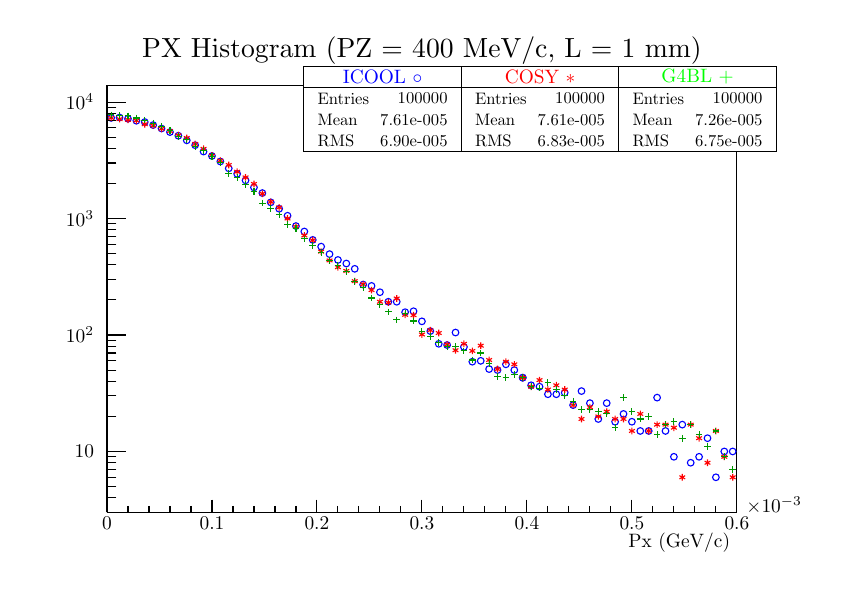
\begin{tikzpicture}
\definecolor{c}{rgb}{1,1,1};
\draw [color=c, fill=c] (0,0) rectangle (20,13.5632);
\draw [color=c, fill=c] (2,1.35632) rectangle (18,12.2069);
\definecolor{c}{rgb}{0,0,0};
\draw [c] (2,1.35632) -- (2,12.2069) -- (18,12.2069) -- (18,1.35632) -- (2,1.35632);
\definecolor{c}{rgb}{1,1,1};
\draw [color=c, fill=c] (2,1.35632) rectangle (18,12.2069);
\definecolor{c}{rgb}{0,0,0};
\draw [c] (2,1.35632) -- (2,12.2069) -- (18,12.2069) -- (18,1.35632) -- (2,1.35632);
\definecolor{c}{rgb}{0,0,1};
\foreach \P in
 {(2.10667,11.375),(2.32,11.3859),(2.53333,11.3538),(2.74667,11.3031),(2.96,11.2702),(3.17333,11.193),(3.38667,11.1061),(3.6,11.016),(3.81333,10.9222),(4.02667,10.8054),(4.24,10.6825),(4.45333,10.5203),(4.66667,10.4082),(4.88,10.2681),(5.09333,10.094
2),(5.30667,9.95505),(5.52,9.78933),(5.73333,9.61017),(5.94667,9.46638),(6.16,9.23014),(6.37333,9.06829),(6.58667,8.89038),(6.8,8.62839),(7.01333,8.49005),(7.22667,8.27755),(7.44,8.10601),(7.65333,7.91579),(7.86667,7.76739),(8.08,7.67688),(8.29333,7.
54188),(8.50667,7.14185),(8.72,7.10823),(8.93333,6.94776),(9.14667,6.7058),(9.36,6.7058),(9.57333,6.44058),(9.78667,6.4649),(10,6.20799),(10.2133,5.95997),(10.4267,5.63711),(10.64,5.60615),(10.8533,5.92378),(11.0667,5.55827),(11.28,5.18326),(11.4933,
5.20485),(11.7067,4.99607),(11.92,4.97063),(12.1333,5.11622),(12.3467,4.97063),(12.56,4.77687)}{\draw[mark options={color=c,fill=c},mark size=2.402402pt,mark=o] plot coordinates {\P};}
\foreach \P in
 {(12.56,4.77687),(12.7733,4.58381),(12.9867,4.54861),(13.2,4.35651),(13.4133,4.35651),(13.6267,4.3973),(13.84,4.08016),(14.0533,4.43683),(14.2667,4.13055),(14.48,3.7276),(14.6933,4.13055),(14.9067,3.65814),(15.12,3.85618),(15.3333,3.65814),(15.5467,
3.42392),(15.76,3.42392),(15.9733,4.27084),(16.1867,3.42392),(16.4,2.76768),(16.6133,3.58472),(16.8267,2.61637),(17.04,2.76768),(17.2533,3.24008),(17.4667,2.24679),(17.68,2.90303),(17.8933,2.90303)}{\draw[mark options={color=c,fill=c},mark
 size=2.402402pt,mark=o] plot coordinates {\P};}
\definecolor{c}{rgb}{1,1,1};
\draw [color=c, fill=c] (7,10.5115) rectangle (11,12.6816);
\definecolor{c}{rgb}{0,0,0};
\draw [c] (7,10.5115) -- (11,10.5115);
\draw [c] (11,10.5115) -- (11,12.6816);
\draw [c] (11,12.6816) -- (7,12.6816);
\draw [c] (7,12.6816) -- (7,10.5115);
\draw[color=blue](9,12.4103) node[scale=0.7, rotate=0]{ICOOL $\circ$};
\draw [c] (7,12.1391) -- (11,12.1391);
\draw [anchor= west] (7.2,11.8678) node[scale=0.6, rotate=0]{Entries };
\draw [anchor= east] (10.8,11.8678) node[scale=0.6, rotate=0]{ 100000};
\draw [anchor= west] (7.2,11.3253) node[scale=0.6, rotate=0]{Mean  };
\draw [anchor= east] (10.8,11.3253) node[scale=0.6, rotate=0]{ 7.61e-005};
\draw [anchor= west] (7.2,10.7828) node[scale=0.6, rotate=0]{RMS   };
\draw [anchor= east] (10.8,10.7828) node[scale=0.6, rotate=0]{ 6.90e-005};
\draw [c] (2,1.35632) -- (18,1.35632);
\draw [anchor= east] (18,0.596782) node[scale=0.7, rotate=0]{Px (GeV/c)};
\draw [c] (2,1.68184) -- (2,1.35632);
\draw [c] (2.53333,1.51908) -- (2.53333,1.35632);
\draw [c] (3.06667,1.51908) -- (3.06667,1.35632);
\draw [c] (3.6,1.51908) -- (3.6,1.35632);
\draw [c] (4.13333,1.51908) -- (4.13333,1.35632);
\draw [c] (4.66667,1.68184) -- (4.66667,1.35632);
\draw [c] (5.2,1.51908) -- (5.2,1.35632);
\draw [c] (5.73333,1.51908) -- (5.73333,1.35632);
\draw [c] (6.26667,1.51908) -- (6.26667,1.35632);
\draw [c] (6.8,1.51908) -- (6.8,1.35632);
\draw [c] (7.33333,1.68184) -- (7.33333,1.35632);
\draw [c] (7.86667,1.51908) -- (7.86667,1.35632);
\draw [c] (8.4,1.51908) -- (8.4,1.35632);
\draw [c] (8.93333,1.51908) -- (8.93333,1.35632);
\draw [c] (9.46667,1.51908) -- (9.46667,1.35632);
\draw [c] (10,1.68184) -- (10,1.35632);
\draw [c] (10.5333,1.51908) -- (10.5333,1.35632);
\draw [c] (11.0667,1.51908) -- (11.0667,1.35632);
\draw [c] (11.6,1.51908) -- (11.6,1.35632);
\draw [c] (12.1333,1.51908) -- (12.1333,1.35632);
\draw [c] (12.6667,1.68184) -- (12.6667,1.35632);
\draw [c] (13.2,1.51908) -- (13.2,1.35632);
\draw [c] (13.7333,1.51908) -- (13.7333,1.35632);
\draw [c] (14.2667,1.51908) -- (14.2667,1.35632);
\draw [c] (14.8,1.51908) -- (14.8,1.35632);
\draw [c] (15.3333,1.68184) -- (15.3333,1.35632);
\draw [c] (15.8667,1.51908) -- (15.8667,1.35632);
\draw [c] (16.4,1.51908) -- (16.4,1.35632);
\draw [c] (16.9333,1.51908) -- (16.9333,1.35632);
\draw [c] (17.4667,1.51908) -- (17.4667,1.35632);
\draw [c] (18,1.68184) -- (18,1.35632);
\draw [anchor=base] (2,0.908736) node[scale=0.7, rotate=0]{0};
\draw [anchor=base] (4.66667,0.908736) node[scale=0.7, rotate=0]{0.1};
\draw [anchor=base] (7.33333,0.908736) node[scale=0.7, rotate=0]{0.2};
\draw [anchor=base] (10,0.908736) node[scale=0.7, rotate=0]{0.3};
\draw [anchor=base] (12.6667,0.908736) node[scale=0.7, rotate=0]{0.4};
\draw [anchor=base] (15.3333,0.908736) node[scale=0.7, rotate=0]{0.5};
\draw [anchor=base] (18,0.908736) node[scale=0.7, rotate=0]{0.6};
\draw [anchor=base west] (18.07,1.35632) node[scale=0.7, rotate=0]{$\times10^{-3}$};
\draw [c] (2,1.35632) -- (2,12.2069);
\draw [c] (2.24,1.7259) -- (2,1.7259);
\draw [c] (2.24,2.01256) -- (2,2.01256);
\draw [c] (2.24,2.24679) -- (2,2.24679);
\draw [c] (2.24,2.44482) -- (2,2.44482);
\draw [c] (2.24,2.61636) -- (2,2.61636);
\draw [c] (2.24,2.76768) -- (2,2.76768);
\draw [c] (2.48,2.90303) -- (2,2.90303);
\draw [anchor= east] (1.844,2.90303) node[scale=0.7, rotate=0]{10};
\draw [c] (2.24,3.7935) -- (2,3.7935);
\draw [c] (2.24,4.31439) -- (2,4.31439);
\draw [c] (2.24,4.68396) -- (2,4.68396);
\draw [c] (2.24,4.97063) -- (2,4.97063);
\draw [c] (2.24,5.20485) -- (2,5.20485);
\draw [c] (2.24,5.40289) -- (2,5.40289);
\draw [c] (2.24,5.57443) -- (2,5.57443);
\draw [c] (2.24,5.72574) -- (2,5.72574);
\draw [c] (2.48,5.8611) -- (2,5.8611);
\draw [anchor= east] (1.844,5.8611) node[scale=0.7, rotate=0]{$10^{2}$};
\draw [c] (2.24,6.75156) -- (2,6.75156);
\draw [c] (2.24,7.27245) -- (2,7.27245);
\draw [c] (2.24,7.64203) -- (2,7.64203);
\draw [c] (2.24,7.9287) -- (2,7.9287);
\draw [c] (2.24,8.16292) -- (2,8.16292);
\draw [c] (2.24,8.36095) -- (2,8.36095);
\draw [c] (2.24,8.5325) -- (2,8.5325);
\draw [c] (2.24,8.68381) -- (2,8.68381);
\draw [c] (2.48,8.81916) -- (2,8.81916);
\draw [anchor= east] (1.844,8.81916) node[scale=0.7, rotate=0]{$10^{3}$};
\draw [c] (2.24,9.70963) -- (2,9.70963);
\draw [c] (2.24,10.2305) -- (2,10.2305);
\draw [c] (2.24,10.6001) -- (2,10.6001);
\draw [c] (2.24,10.8868) -- (2,10.8868);
\draw [c] (2.24,11.121) -- (2,11.121);
\draw [c] (2.24,11.319) -- (2,11.319);
\draw [c] (2.24,11.4906) -- (2,11.4906);
\draw [c] (2.24,11.6419) -- (2,11.6419);
\draw [c] (2.48,11.7772) -- (2,11.7772);
\draw [anchor= east] (1.844,11.7772) node[scale=0.7, rotate=0]{$10^{4}$};
\definecolor{c}{rgb}{1,1,1};
\draw [color=c, fill=c] (7,10.5115) rectangle (11,12.6816);
\definecolor{c}{rgb}{0,0,0};
\draw [c] (7,10.5115) -- (11,10.5115);
\draw [c] (11,10.5115) -- (11,12.6816);
\draw [c] (11,12.6816) -- (7,12.6816);
\draw [c] (7,12.6816) -- (7,10.5115);
\draw[color=blue](9,12.4103) node[scale=0.7, rotate=0]{ICOOL $\circ$};
\draw [c] (7,12.1391) -- (11,12.1391);
\draw [anchor= west] (7.2,11.8678) node[scale=0.6, rotate=0]{Entries };
\draw [anchor= east] (10.8,11.8678) node[scale=0.6, rotate=0]{ 100000};
\draw [anchor= west] (7.2,11.3253) node[scale=0.6, rotate=0]{Mean  };
\draw [anchor= east] (10.8,11.3253) node[scale=0.6, rotate=0]{ 7.61e-005};
\draw [anchor= west] (7.2,10.7828) node[scale=0.6, rotate=0]{RMS   };
\draw [anchor= east] (10.8,10.7828) node[scale=0.6, rotate=0]{ 6.90e-005};
\draw (10,13.0816) node[scale=1, rotate=0]{PX Histogram (PZ = 400 MeV/c, L = 1 mm)};
\definecolor{c}{rgb}{1,0,0};
\foreach \P in
 {(2.10667,11.375),(2.32,11.3445),(2.53333,11.3263),(2.74667,11.308),(2.96,11.2149),(3.17333,11.1798),(3.38667,11.0996),(3.6,11.0408),(3.81333,10.9334),(4.02667,10.8653),(4.24,10.714),(4.45333,10.5901),(4.66667,10.4193),(4.88,10.2912),(5.09333,10.179
),(5.30667,10.0081),(5.52,9.86493),(5.73333,9.69737),(5.94667,9.45076),(6.16,9.24314),(6.37333,9.10068),(6.58667,8.82045),(6.8,8.60887),(7.01333,8.38819),(7.22667,8.26772),(7.44,7.97908),(7.65333,7.75568),(7.86667,7.58288),(8.08,7.48871),(8.29333,7.2
289),(8.50667,7.1513),(8.72,7.00175),(8.93333,6.7058),(9.14667,6.68567),(9.36,6.78954),(9.57333,6.37339),(9.78667,6.36474),(10,5.87388),(10.2133,5.98354),(10.4267,5.91148),(10.64,5.62173),(10.8533,5.47428),(11.0667,5.63711),(11.28,5.4568),(11.4933,5.
59039),(11.7067,5.22609),(11.92,4.99607),(12.1333,5.18326),(12.3467,5.11622),(12.56,4.77687)}{\draw[mark options={color=c,fill=c},mark size=2.402402pt,mark=asterisk] plot coordinates {\P};}
\foreach \P in
 {(12.56,4.77687),(12.7733,4.54861),(12.9867,4.71569),(13.2,4.47518),(13.4133,4.58381),(13.6267,4.47518),(13.84,4.08016),(14.0533,3.7276),(14.2667,4.02772),(14.48,3.7935),(14.6933,3.91594),(14.9067,3.7276),(15.12,3.7276),(15.3333,3.42392),(15.5467,3.
85618),(15.76,3.42392),(15.9733,3.58472),(16.1867,3.58472),(16.4,3.50683),(16.6133,2.24679),(16.8267,3.58472),(17.04,3.24008),(17.2533,2.61637),(17.4667,3.42392),(17.68,2.76768),(17.8933,2.24679)}{\draw[mark options={color=c,fill=c},mark
 size=2.402402pt,mark=asterisk] plot coordinates {\P};}
\definecolor{c}{rgb}{1,1,1};
\draw [color=c, fill=c] (11,10.5115) rectangle (15,12.6816);
\definecolor{c}{rgb}{0,0,0};
\draw [c] (11,10.5115) -- (15,10.5115);
\draw [c] (15,10.5115) -- (15,12.6816);
\draw [c] (15,12.6816) -- (11,12.6816);
\draw [c] (11,12.6816) -- (11,10.5115);
\draw [color=red](13,12.4103) node[scale=0.7, rotate=0]{COSY $*$};
\draw [c] (11,12.1391) -- (15,12.1391);
\draw [anchor= west] (11.2,11.8678) node[scale=0.6, rotate=0]{Entries };
\draw [anchor= east] (14.8,11.8678) node[scale=0.6, rotate=0]{ 100000};
\draw [anchor= west] (11.2,11.3253) node[scale=0.6, rotate=0]{Mean  };
\draw [anchor= east] (14.8,11.3253) node[scale=0.6, rotate=0]{ 7.61e-005};
\draw [anchor= west] (11.2,10.7828) node[scale=0.6, rotate=0]{RMS   };
\draw [anchor= east] (14.8,10.7828) node[scale=0.6, rotate=0]{ 6.83e-005};
\definecolor{c}{rgb}{1,1,1};
\draw [color=c, fill=c] (11,10.5115) rectangle (15,12.6816);
\definecolor{c}{rgb}{0,0,0};
\draw [c] (11,10.5115) -- (15,10.5115);
\draw [c] (15,10.5115) -- (15,12.6816);
\draw [c] (15,12.6816) -- (11,12.6816);
\draw [c] (11,12.6816) -- (11,10.5115);
\draw [color=red](13,12.4103) node[scale=0.7, rotate=0]{COSY $*$};
\draw [c] (11,12.1391) -- (15,12.1391);
\draw [anchor= west] (11.2,11.8678) node[scale=0.6, rotate=0]{Entries };
\draw [anchor= east] (14.8,11.8678) node[scale=0.6, rotate=0]{ 100000};
\draw [anchor= west] (11.2,11.3253) node[scale=0.6, rotate=0]{Mean  };
\draw [anchor= east] (14.8,11.3253) node[scale=0.6, rotate=0]{ 7.61e-005};
\draw [anchor= west] (11.2,10.7828) node[scale=0.6, rotate=0]{RMS   };
\draw [anchor= east] (14.8,10.7828) node[scale=0.6, rotate=0]{ 6.83e-005};
\definecolor{c}{rgb}{0,0.6,0};
\foreach \P in
 {(2.10667,11.4531),(2.32,11.438),(2.53333,11.4255),(2.74667,11.3735),(2.96,11.3179),(3.17333,11.2395),(3.38667,11.167),(3.6,11.0497),(3.81333,10.9011),(4.02667,10.8182),(4.24,10.653),(4.45333,10.5413),(4.66667,10.3936),(4.88,10.245),(5.09333,9.96824
),(5.30667,9.86323),(5.52,9.68368),(5.73333,9.50085),(5.94667,9.21134),(6.16,9.07988),(6.37333,8.91207),(6.58667,8.67378),(6.8,8.57359),(7.01333,8.30276),(7.22667,8.1304),(7.44,7.96417),(7.65333,7.74684),(7.86667,7.62262),(8.08,7.48145),(8.29333,7.21
554),(8.50667,7.07371),(8.72,6.80195),(8.93333,6.63041),(9.14667,6.44874),(9.36,6.24663),(9.57333,6.4158),(9.78667,6.21776),(10,5.95997),(10.2133,5.82197),(10.4267,5.66734),(10.64,5.55827),(10.8533,5.57443),(11.0667,5.4568),(11.28,5.22609),(11.4933,5
.40289),(11.7067,5.13896),(11.92,4.80641),(12.1333,4.77687),(12.3467,4.86351),(12.56,4.77687)}{\draw[mark options={color=c,fill=c},mark size=2.402402pt,mark=+] plot coordinates {\P};}
\foreach \P in
 {(12.56,4.77687),(12.7733,4.54861),(12.9867,4.51242),(13.2,4.65144),(13.4133,4.47518),(13.6267,4.31439),(13.84,4.17903),(14.0533,3.97305),(14.2667,3.97305),(14.48,3.91594),(14.6933,3.85618),(14.9067,3.50683),(15.12,4.27084),(15.3333,3.91594),(15.546
7,3.7276),(15.76,3.7935),(15.9733,3.33529),(16.1867,3.58472),(16.4,3.65814),(16.6133,3.24008),(16.8267,3.58472),(17.04,3.33529),(17.2533,3.02547),(17.4667,3.42392),(17.68,2.76768),(17.8933,2.44482)}{\draw[mark options={color=c,fill=c},mark
 size=2.402402pt,mark=+] plot coordinates {\P};}
\definecolor{c}{rgb}{1,1,1};
\draw [color=c, fill=c] (15,10.5115) rectangle (19,12.6816);
\definecolor{c}{rgb}{0,0,0};
\draw [c] (15,10.5115) -- (19,10.5115);
\draw [c] (19,10.5115) -- (19,12.6816);
\draw [c] (19,12.6816) -- (15,12.6816);
\draw [c] (15,12.6816) -- (15,10.5115);
\draw [color=green](17,12.4103) node[scale=0.7, rotate=0]{G4BL $+$};
\draw [c] (15,12.1391) -- (19,12.1391);
\draw [anchor= west] (15.2,11.8678) node[scale=0.6, rotate=0]{Entries };
\draw [anchor= east] (18.8,11.8678) node[scale=0.6, rotate=0]{ 100000};
\draw [anchor= west] (15.2,11.3253) node[scale=0.6, rotate=0]{Mean  };
\draw [anchor= east] (18.8,11.3253) node[scale=0.6, rotate=0]{ 7.26e-005};
\draw [anchor= west] (15.2,10.7828) node[scale=0.6, rotate=0]{RMS   };
\draw [anchor= east] (18.8,10.7828) node[scale=0.6, rotate=0]{ 6.75e-005};
\definecolor{c}{rgb}{1,1,1};
\draw [color=c, fill=c] (15,10.5115) rectangle (19,12.6816);
\definecolor{c}{rgb}{0,0,0};
\draw [c] (15,10.5115) -- (19,10.5115);
\draw [c] (19,10.5115) -- (19,12.6816);
\draw [c] (19,12.6816) -- (15,12.6816);
\draw [c] (15,12.6816) -- (15,10.5115);
\draw [color=green](17,12.4103) node[scale=0.7, rotate=0]{G4BL $+$};
\draw [c] (15,12.1391) -- (19,12.1391);
\draw [anchor= west] (15.2,11.8678) node[scale=0.6, rotate=0]{Entries };
\draw [anchor= east] (18.8,11.8678) node[scale=0.6, rotate=0]{ 100000};
\draw [anchor= west] (15.2,11.3253) node[scale=0.6, rotate=0]{Mean  };
\draw [anchor= east] (18.8,11.3253) node[scale=0.6, rotate=0]{ 7.26e-005};
\draw [anchor= west] (15.2,10.7828) node[scale=0.6, rotate=0]{RMS   };
\draw [anchor= east] (18.8,10.7828) node[scale=0.6, rotate=0]{ 6.75e-005};
\end{tikzpicture}
}\\
\frame{\pgfdeclareplotmark{cross} {
\pgfpathmoveto{\pgfpoint{-0.3\pgfplotmarksize}{\pgfplotmarksize}}
\pgfpathlineto{\pgfpoint{+0.3\pgfplotmarksize}{\pgfplotmarksize}}
\pgfpathlineto{\pgfpoint{+0.3\pgfplotmarksize}{0.3\pgfplotmarksize}}
\pgfpathlineto{\pgfpoint{+1\pgfplotmarksize}{0.3\pgfplotmarksize}}
\pgfpathlineto{\pgfpoint{+1\pgfplotmarksize}{-0.3\pgfplotmarksize}}
\pgfpathlineto{\pgfpoint{+0.3\pgfplotmarksize}{-0.3\pgfplotmarksize}}
\pgfpathlineto{\pgfpoint{+0.3\pgfplotmarksize}{-1.\pgfplotmarksize}}
\pgfpathlineto{\pgfpoint{-0.3\pgfplotmarksize}{-1.\pgfplotmarksize}}
\pgfpathlineto{\pgfpoint{-0.3\pgfplotmarksize}{-0.3\pgfplotmarksize}}
\pgfpathlineto{\pgfpoint{-1.\pgfplotmarksize}{-0.3\pgfplotmarksize}}
\pgfpathlineto{\pgfpoint{-1.\pgfplotmarksize}{0.3\pgfplotmarksize}}
\pgfpathlineto{\pgfpoint{-0.3\pgfplotmarksize}{0.3\pgfplotmarksize}}
\pgfpathclose
\pgfusepathqstroke
}
\pgfdeclareplotmark{cross*} {
\pgfpathmoveto{\pgfpoint{-0.3\pgfplotmarksize}{\pgfplotmarksize}}
\pgfpathlineto{\pgfpoint{+0.3\pgfplotmarksize}{\pgfplotmarksize}}
\pgfpathlineto{\pgfpoint{+0.3\pgfplotmarksize}{0.3\pgfplotmarksize}}
\pgfpathlineto{\pgfpoint{+1\pgfplotmarksize}{0.3\pgfplotmarksize}}
\pgfpathlineto{\pgfpoint{+1\pgfplotmarksize}{-0.3\pgfplotmarksize}}
\pgfpathlineto{\pgfpoint{+0.3\pgfplotmarksize}{-0.3\pgfplotmarksize}}
\pgfpathlineto{\pgfpoint{+0.3\pgfplotmarksize}{-1.\pgfplotmarksize}}
\pgfpathlineto{\pgfpoint{-0.3\pgfplotmarksize}{-1.\pgfplotmarksize}}
\pgfpathlineto{\pgfpoint{-0.3\pgfplotmarksize}{-0.3\pgfplotmarksize}}
\pgfpathlineto{\pgfpoint{-1.\pgfplotmarksize}{-0.3\pgfplotmarksize}}
\pgfpathlineto{\pgfpoint{-1.\pgfplotmarksize}{0.3\pgfplotmarksize}}
\pgfpathlineto{\pgfpoint{-0.3\pgfplotmarksize}{0.3\pgfplotmarksize}}
\pgfpathclose
\pgfusepathqfillstroke
}
\pgfdeclareplotmark{newstar} {
\pgfpathmoveto{\pgfqpoint{0pt}{\pgfplotmarksize}}
\pgfpathlineto{\pgfqpointpolar{44}{0.5\pgfplotmarksize}}
\pgfpathlineto{\pgfqpointpolar{18}{\pgfplotmarksize}}
\pgfpathlineto{\pgfqpointpolar{-20}{0.5\pgfplotmarksize}}
\pgfpathlineto{\pgfqpointpolar{-54}{\pgfplotmarksize}}
\pgfpathlineto{\pgfqpointpolar{-90}{0.5\pgfplotmarksize}}
\pgfpathlineto{\pgfqpointpolar{234}{\pgfplotmarksize}}
\pgfpathlineto{\pgfqpointpolar{198}{0.5\pgfplotmarksize}}
\pgfpathlineto{\pgfqpointpolar{162}{\pgfplotmarksize}}
\pgfpathlineto{\pgfqpointpolar{134}{0.5\pgfplotmarksize}}
\pgfpathclose
\pgfusepathqstroke
}
\pgfdeclareplotmark{newstar*} {
\pgfpathmoveto{\pgfqpoint{0pt}{\pgfplotmarksize}}
\pgfpathlineto{\pgfqpointpolar{44}{0.5\pgfplotmarksize}}
\pgfpathlineto{\pgfqpointpolar{18}{\pgfplotmarksize}}
\pgfpathlineto{\pgfqpointpolar{-20}{0.5\pgfplotmarksize}}
\pgfpathlineto{\pgfqpointpolar{-54}{\pgfplotmarksize}}
\pgfpathlineto{\pgfqpointpolar{-90}{0.5\pgfplotmarksize}}
\pgfpathlineto{\pgfqpointpolar{234}{\pgfplotmarksize}}
\pgfpathlineto{\pgfqpointpolar{198}{0.5\pgfplotmarksize}}
\pgfpathlineto{\pgfqpointpolar{162}{\pgfplotmarksize}}
\pgfpathlineto{\pgfqpointpolar{134}{0.5\pgfplotmarksize}}
\pgfpathclose
\pgfusepathqfillstroke
}
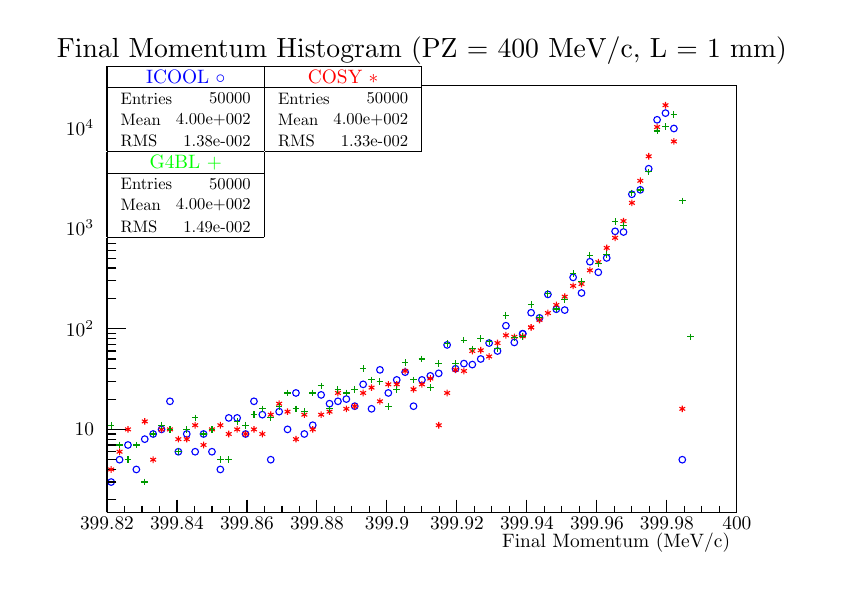
\begin{tikzpicture}
\definecolor{c}{rgb}{1,1,1};
\draw [color=c, fill=c] (0,0) rectangle (20,13.5632);
\draw [color=c, fill=c] (2,1.35632) rectangle (18,12.2069);
\definecolor{c}{rgb}{0,0,0};
\draw [c] (2,1.35632) -- (2,12.2069) -- (18,12.2069) -- (18,1.35632) -- (2,1.35632);
\definecolor{c}{rgb}{1,1,1};
\draw [color=c, fill=c] (2,1.35632) rectangle (18,12.2069);
\definecolor{c}{rgb}{0,0,0};
\draw [c] (2,1.35632) -- (2,12.2069) -- (18,12.2069) -- (18,1.35632) -- (2,1.35632);
\definecolor{c}{rgb}{0,0,1};
\foreach \P in
 {(2.10667,2.12635),(2.32,2.69383),(2.53333,3.06762),(2.74667,2.44594),(2.96,3.21596),(3.17333,3.34681),(3.38667,3.46385),(3.6,4.1769),(3.81333,2.89637),(4.02667,3.34681),(4.24,2.89637),(4.45333,3.34681),(4.66667,2.89637),(4.88,2.44594),(5.09333,3.75
532),(5.30667,3.75532),(5.52,3.34681),(5.73333,4.1769),(5.94667,3.83765),(6.16,2.69383),(6.37333,3.91429),(6.58667,3.46385),(6.8,4.38914),(7.01333,3.34681),(7.22667,3.56974),(7.44,4.33976),(7.65333,4.11683),(7.86667,4.1769),(8.08,4.23388),(8.29333,4.
05334),(8.50667,4.60767),(8.72,3.98599),(8.93333,4.97578),(9.14667,4.38914),(9.36,4.72074),(9.57333,4.9173),(9.78667,4.05334),(10,4.72074),(10.2133,4.82336),(10.4267,4.88686),(10.64,5.6096),(10.8533,5.00391),(11.0667,5.13475),(11.28,5.10979),(11.4933
,5.2518),(11.7067,5.65688),(11.92,5.45434),(12.1333,6.09699),(12.3467,5.67221),(12.56,5.89236)}{\draw[mark options={color=c,fill=c},mark size=2.402402pt,mark=o] plot coordinates {\P};}
\foreach \P in
 {(12.56,5.89236),(12.7733,6.42691),(12.9867,6.29606),(13.2,6.89267),(13.4133,6.51583),(13.6267,6.49426),(13.84,7.32435),(14.0533,6.92762),(14.2667,7.72196),(14.48,7.45405),(14.6933,7.81862),(14.9067,8.49438),(15.12,8.47746),(15.3333,9.43583),(15.546
7,9.54865),(15.76,10.0843),(15.9733,11.3275),(16.1867,11.4969),(16.4,11.1062),(16.6133,2.69383)}{\draw[mark options={color=c,fill=c},mark size=2.402402pt,mark=o] plot coordinates {\P};}
\definecolor{c}{rgb}{1,1,1};
\draw [color=c, fill=c] (2,10.5115) rectangle (6,12.6816);
\definecolor{c}{rgb}{0,0,0};
\draw [c] (2,10.5115) -- (6,10.5115);
\draw [c] (6,10.5115) -- (6,12.6816);
\draw [c] (6,12.6816) -- (2,12.6816);
\draw [c] (2,12.6816) -- (2,10.5115);
\draw[color=blue](4,12.4103) node[scale=0.7, rotate=0]{ICOOL $\circ$};
\draw [c] (2,12.1391) -- (6,12.1391);
\draw [anchor= west] (2.2,11.8678) node[scale=0.6, rotate=0]{Entries };
\draw [anchor= east] (5.8,11.8678) node[scale=0.6, rotate=0]{ 50000};
\draw [anchor= west] (2.2,11.3253) node[scale=0.6, rotate=0]{Mean  };
\draw [anchor= east] (5.8,11.3253) node[scale=0.6, rotate=0]{ 4.00e+002};
\draw [anchor= west] (2.2,10.7828) node[scale=0.6, rotate=0]{RMS   };
\draw [anchor= east] (5.8,10.7828) node[scale=0.6, rotate=0]{ 1.38e-002};
\draw [c] (2,1.35632) -- (18,1.35632);
\draw [anchor= east] (18,0.596782) node[scale=0.7, rotate=0]{Final Momentum (MeV/c)};
\draw [c] (2,1.68184) -- (2,1.35632);
\draw [c] (2.44444,1.51908) -- (2.44444,1.35632);
\draw [c] (2.88889,1.51908) -- (2.88889,1.35632);
\draw [c] (3.33333,1.51908) -- (3.33333,1.35632);
\draw [c] (3.77778,1.68184) -- (3.77778,1.35632);
\draw [c] (4.22222,1.51908) -- (4.22222,1.35632);
\draw [c] (4.66667,1.51908) -- (4.66667,1.35632);
\draw [c] (5.11111,1.51908) -- (5.11111,1.35632);
\draw [c] (5.55556,1.68184) -- (5.55556,1.35632);
\draw [c] (6,1.51908) -- (6,1.35632);
\draw [c] (6.44444,1.51908) -- (6.44444,1.35632);
\draw [c] (6.88889,1.51908) -- (6.88889,1.35632);
\draw [c] (7.33333,1.68184) -- (7.33333,1.35632);
\draw [c] (7.77778,1.51908) -- (7.77778,1.35632);
\draw [c] (8.22222,1.51908) -- (8.22222,1.35632);
\draw [c] (8.66667,1.51908) -- (8.66667,1.35632);
\draw [c] (9.11111,1.68184) -- (9.11111,1.35632);
\draw [c] (9.55556,1.51908) -- (9.55556,1.35632);
\draw [c] (10,1.51908) -- (10,1.35632);
\draw [c] (10.4444,1.51908) -- (10.4444,1.35632);
\draw [c] (10.8889,1.68184) -- (10.8889,1.35632);
\draw [c] (11.3333,1.51908) -- (11.3333,1.35632);
\draw [c] (11.7778,1.51908) -- (11.7778,1.35632);
\draw [c] (12.2222,1.51908) -- (12.2222,1.35632);
\draw [c] (12.6667,1.68184) -- (12.6667,1.35632);
\draw [c] (13.1111,1.51908) -- (13.1111,1.35632);
\draw [c] (13.5556,1.51908) -- (13.5556,1.35632);
\draw [c] (14,1.51908) -- (14,1.35632);
\draw [c] (14.4444,1.68184) -- (14.4444,1.35632);
\draw [c] (14.8889,1.51908) -- (14.8889,1.35632);
\draw [c] (15.3333,1.51908) -- (15.3333,1.35632);
\draw [c] (15.7778,1.51908) -- (15.7778,1.35632);
\draw [c] (16.2222,1.68184) -- (16.2222,1.35632);
\draw [c] (16.6667,1.51908) -- (16.6667,1.35632);
\draw [c] (17.1111,1.51908) -- (17.1111,1.35632);
\draw [c] (17.5556,1.51908) -- (17.5556,1.35632);
\draw [c] (18,1.68184) -- (18,1.35632);
\draw [anchor=base] (2,0.908736) node[scale=0.7, rotate=0]{399.82};
\draw [anchor=base] (3.77778,0.908736) node[scale=0.7, rotate=0]{399.84};
\draw [anchor=base] (5.55556,0.908736) node[scale=0.7, rotate=0]{399.86};
\draw [anchor=base] (7.33333,0.908736) node[scale=0.7, rotate=0]{399.88};
\draw [anchor=base] (9.11111,0.908736) node[scale=0.7, rotate=0]{399.9};
\draw [anchor=base] (10.8889,0.908736) node[scale=0.7, rotate=0]{399.92};
\draw [anchor=base] (12.6667,0.908736) node[scale=0.7, rotate=0]{399.94};
\draw [anchor=base] (14.4444,0.908736) node[scale=0.7, rotate=0]{399.96};
\draw [anchor=base] (16.2222,0.908736) node[scale=0.7, rotate=0]{399.98};
\draw [anchor=base] (18,0.908736) node[scale=0.7, rotate=0]{400};
\draw [c] (2,1.35632) -- (2,12.2069);
\draw [c] (2.24,1.67591) -- (2,1.67591);
\draw [c] (2.24,2.12634) -- (2,2.12634);
\draw [c] (2.24,2.44593) -- (2,2.44593);
\draw [c] (2.24,2.69383) -- (2,2.69383);
\draw [c] (2.24,2.89637) -- (2,2.89637);
\draw [c] (2.24,3.06762) -- (2,3.06762);
\draw [c] (2.24,3.21596) -- (2,3.21596);
\draw [c] (2.24,3.34681) -- (2,3.34681);
\draw [c] (2.48,3.46385) -- (2,3.46385);
\draw [anchor= east] (1.844,3.46385) node[scale=0.7, rotate=0]{10};
\draw [c] (2.24,4.23388) -- (2,4.23388);
\draw [c] (2.24,4.68431) -- (2,4.68431);
\draw [c] (2.24,5.0039) -- (2,5.0039);
\draw [c] (2.24,5.2518) -- (2,5.2518);
\draw [c] (2.24,5.45434) -- (2,5.45434);
\draw [c] (2.24,5.62559) -- (2,5.62559);
\draw [c] (2.24,5.77393) -- (2,5.77393);
\draw [c] (2.24,5.90478) -- (2,5.90478);
\draw [c] (2.48,6.02182) -- (2,6.02182);
\draw [anchor= east] (1.844,6.02182) node[scale=0.7, rotate=0]{$10^{2}$};
\draw [c] (2.24,6.79185) -- (2,6.79185);
\draw [c] (2.24,7.24228) -- (2,7.24228);
\draw [c] (2.24,7.56187) -- (2,7.56187);
\draw [c] (2.24,7.80977) -- (2,7.80977);
\draw [c] (2.24,8.01231) -- (2,8.01231);
\draw [c] (2.24,8.18356) -- (2,8.18356);
\draw [c] (2.24,8.3319) -- (2,8.3319);
\draw [c] (2.24,8.46274) -- (2,8.46274);
\draw [c] (2.48,8.57979) -- (2,8.57979);
\draw [anchor= east] (1.844,8.57979) node[scale=0.7, rotate=0]{$10^{3}$};
\draw [c] (2.24,9.34982) -- (2,9.34982);
\draw [c] (2.24,9.80025) -- (2,9.80025);
\draw [c] (2.24,10.1198) -- (2,10.1198);
\draw [c] (2.24,10.3677) -- (2,10.3677);
\draw [c] (2.24,10.5703) -- (2,10.5703);
\draw [c] (2.24,10.7415) -- (2,10.7415);
\draw [c] (2.24,10.8899) -- (2,10.8899);
\draw [c] (2.24,11.0207) -- (2,11.0207);
\draw [c] (2.48,11.1378) -- (2,11.1378);
\draw [anchor= east] (1.844,11.1378) node[scale=0.7, rotate=0]{$10^{4}$};
\draw [c] (2.24,11.9078) -- (2,11.9078);
\definecolor{c}{rgb}{1,1,1};
\draw [color=c, fill=c] (2,10.5115) rectangle (6,12.6816);
\definecolor{c}{rgb}{0,0,0};
\draw [c] (2,10.5115) -- (6,10.5115);
\draw [c] (6,10.5115) -- (6,12.6816);
\draw [c] (6,12.6816) -- (2,12.6816);
\draw [c] (2,12.6816) -- (2,10.5115);
\draw[color=blue](4,12.4103) node[scale=0.7, rotate=0]{ICOOL $\circ$};
\draw [c] (2,12.1391) -- (6,12.1391);
\draw [anchor= west] (2.2,11.8678) node[scale=0.6, rotate=0]{Entries };
\draw [anchor= east] (5.8,11.8678) node[scale=0.6, rotate=0]{ 50000};
\draw [anchor= west] (2.2,11.3253) node[scale=0.6, rotate=0]{Mean  };
\draw [anchor= east] (5.8,11.3253) node[scale=0.6, rotate=0]{ 4.00e+002};
\draw [anchor= west] (2.2,10.7828) node[scale=0.6, rotate=0]{RMS   };
\draw [anchor= east] (5.8,10.7828) node[scale=0.6, rotate=0]{ 1.38e-002};
\draw (10,13.0816) node[scale=1, rotate=0]{Final Momentum Histogram (PZ = 400 MeV/c, L = 1 mm)};
\definecolor{c}{rgb}{1,0,0};
\foreach \P in
 {(2.10667,2.44594),(2.32,2.89637),(2.53333,3.46385),(2.96,3.6664),(3.17333,2.69383),(3.38667,3.46385),(3.6,3.46385),(3.81333,3.21596),(4.02667,3.21596),(4.24,3.56974),(4.45333,3.06762),(4.66667,3.46385),(4.88,3.56974),(5.09333,3.34681),(5.30667,3.46
385),(5.52,3.34681),(5.73333,3.46385),(5.94667,3.34681),(6.16,3.83765),(6.37333,4.11683),(6.58667,3.91429),(6.8,3.21596),(7.01333,3.83765),(7.22667,3.46385),(7.44,3.83765),(7.65333,3.91429),(7.86667,4.38914),(8.08,3.98599),(8.29333,4.05334),(8.50667,
4.38914),(8.72,4.52534),(8.93333,4.1769),(9.14667,4.60767),(9.36,4.60767),(9.57333,4.94692),(9.78667,4.48177),(10,4.60767),(10.2133,4.75601),(10.4267,3.56974),(10.64,4.38914),(10.8533,4.97578),(11.0667,4.94692),(11.28,5.45434),(11.4933,5.4727),(11.70
67,5.31653),(11.92,5.65688),(12.1333,5.85427),(12.3467,5.81483),(12.56,5.82813),(12.7733,6.05466)}{\draw[mark options={color=c,fill=c},mark size=2.402402pt,mark=asterisk] plot coordinates {\P};}
\foreach \P in
 {(12.7733,6.05466),(12.9867,6.24273),(13.2,6.41917),(13.4133,6.6243),(13.6267,6.83542),(13.84,7.10866),(14.0533,7.15768),(14.2667,7.50489),(14.48,7.7123),(14.6933,8.07354),(14.9067,8.32912),(15.12,8.75421),(15.3333,9.21723),(15.5467,9.77781),(15.76,
10.3997),(15.9733,11.1433),(16.1867,11.6984),(16.4,10.7784),(16.6133,3.98599)}{\draw[mark options={color=c,fill=c},mark size=2.402402pt,mark=asterisk] plot coordinates {\P};}
\definecolor{c}{rgb}{1,1,1};
\draw [color=c, fill=c] (6,10.5115) rectangle (10,12.6816);
\definecolor{c}{rgb}{0,0,0};
\draw [c] (6,10.5115) -- (10,10.5115);
\draw [c] (10,10.5115) -- (10,12.6816);
\draw [c] (10,12.6816) -- (6,12.6816);
\draw [c] (6,12.6816) -- (6,10.5115);
\draw [color=red](8,12.4103) node[scale=0.7, rotate=0]{COSY $*$};
\draw [c] (6,12.1391) -- (10,12.1391);
\draw [anchor= west] (6.2,11.8678) node[scale=0.6, rotate=0]{Entries };
\draw [anchor= east] (9.8,11.8678) node[scale=0.6, rotate=0]{ 50000};
\draw [anchor= west] (6.2,11.3253) node[scale=0.6, rotate=0]{Mean  };
\draw [anchor= east] (9.8,11.3253) node[scale=0.6, rotate=0]{ 4.00e+002};
\draw [anchor= west] (6.2,10.7828) node[scale=0.6, rotate=0]{RMS   };
\draw [anchor= east] (9.8,10.7828) node[scale=0.6, rotate=0]{ 1.33e-002};
\definecolor{c}{rgb}{1,1,1};
\draw [color=c, fill=c] (6,10.5115) rectangle (10,12.6816);
\definecolor{c}{rgb}{0,0,0};
\draw [c] (6,10.5115) -- (10,10.5115);
\draw [c] (10,10.5115) -- (10,12.6816);
\draw [c] (10,12.6816) -- (6,12.6816);
\draw [c] (6,12.6816) -- (6,10.5115);
\draw [color=red](8,12.4103) node[scale=0.7, rotate=0]{COSY $*$};
\draw [c] (6,12.1391) -- (10,12.1391);
\draw [anchor= west] (6.2,11.8678) node[scale=0.6, rotate=0]{Entries };
\draw [anchor= east] (9.8,11.8678) node[scale=0.6, rotate=0]{ 50000};
\draw [anchor= west] (6.2,11.3253) node[scale=0.6, rotate=0]{Mean  };
\draw [anchor= east] (9.8,11.3253) node[scale=0.6, rotate=0]{ 4.00e+002};
\draw [anchor= west] (6.2,10.7828) node[scale=0.6, rotate=0]{RMS   };
\draw [anchor= east] (9.8,10.7828) node[scale=0.6, rotate=0]{ 1.33e-002};
\definecolor{c}{rgb}{0,0.6,0};
\foreach \P in
 {(2.10667,3.56974),(2.32,3.06762),(2.53333,2.69383),(2.74667,3.06762),(2.96,2.12635),(3.17333,3.34681),(3.38667,3.56974),(3.6,3.46385),(3.81333,2.89637),(4.02667,3.46385),(4.24,3.75532),(4.45333,3.34681),(4.66667,3.46385),(4.88,2.69383),(5.09333,2.6
9383),(5.30667,3.6664),(5.52,3.56974),(5.73333,3.83765),(5.94667,3.98599),(6.16,3.75532),(6.37333,4.05334),(6.58667,4.38914),(6.8,3.98599),(7.01333,3.91429),(7.22667,4.38914),(7.44,4.56727),(7.65333,3.98599),(7.86667,4.48177),(8.08,4.38914),(8.29333,
4.48177),(8.50667,5.00391),(8.72,4.72074),(8.93333,4.68432),(9.14667,4.05334),(9.36,4.48177),(9.57333,5.15917),(9.78667,4.72074),(10,5.2518),(10.2133,4.52534),(10.4267,5.13475),(10.64,5.64135),(10.8533,5.13475),(11.0667,5.73147),(11.28,5.50854),(11.4
933,5.77393),(11.7067,5.68732),(11.92,5.50854),(12.1333,6.36341),(12.3467,5.78773),(12.56,5.82813)}{\draw[mark options={color=c,fill=c},mark size=2.402402pt,mark=+] plot coordinates {\P};}
\foreach \P in
 {(12.56,5.82813),(12.7733,6.64351),(12.9867,6.31329),(13.2,6.90778),(13.4133,6.52293),(13.6267,6.76941),(13.84,7.42616),(14.0533,7.21984),(14.2667,7.89114),(14.48,7.66776),(14.6933,7.90346),(14.9067,8.74563),(15.12,8.64557),(15.3333,9.47224),(15.546
7,9.54493),(15.76,10.0031),(15.9733,11.043),(16.1867,11.1496),(16.4,11.4623),(16.6133,9.26621),(16.8267,5.81483)}{\draw[mark options={color=c,fill=c},mark size=2.402402pt,mark=+] plot coordinates {\P};}
\definecolor{c}{rgb}{1,1,1};
\draw [color=c, fill=c] (2,8.34138) rectangle (6,10.5115);
\definecolor{c}{rgb}{0,0,0};
\draw [c] (2,8.34138) -- (6,8.34138);
\draw [c] (6,8.34138) -- (6,10.5115);
\draw [c] (6,10.5115) -- (2,10.5115);
\draw [c] (2,10.5115) -- (2,8.34138);
\draw [color=green](4,10.2402) node[scale=0.7, rotate=0]{G4BL $+$};
\draw [c] (2,9.96897) -- (6,9.96897);
\draw [anchor= west] (2.2,9.6977) node[scale=0.6, rotate=0]{Entries };
\draw [anchor= east] (5.8,9.6977) node[scale=0.6, rotate=0]{ 50000};
\draw [anchor= west] (2.2,9.15517) node[scale=0.6, rotate=0]{Mean  };
\draw [anchor= east] (5.8,9.15517) node[scale=0.6, rotate=0]{ 4.00e+002};
\draw [anchor= west] (2.2,8.61264) node[scale=0.6, rotate=0]{RMS   };
\draw [anchor= east] (5.8,8.61264) node[scale=0.6, rotate=0]{ 1.49e-002};
\definecolor{c}{rgb}{1,1,1};
\draw [color=c, fill=c] (2,8.34138) rectangle (6,10.5115);
\definecolor{c}{rgb}{0,0,0};
\draw [c] (2,8.34138) -- (6,8.34138);
\draw [c] (6,8.34138) -- (6,10.5115);
\draw [c] (6,10.5115) -- (2,10.5115);
\draw [c] (2,10.5115) -- (2,8.34138);
\draw [color=green](4,10.2402) node[scale=0.7, rotate=0]{G4BL $+$};
\draw [c] (2,9.96897) -- (6,9.96897);
\draw [anchor= west] (2.2,9.6977) node[scale=0.6, rotate=0]{Entries };
\draw [anchor= east] (5.8,9.6977) node[scale=0.6, rotate=0]{ 50000};
\draw [anchor= west] (2.2,9.15517) node[scale=0.6, rotate=0]{Mean  };
\draw [anchor= east] (5.8,9.15517) node[scale=0.6, rotate=0]{ 4.00e+002};
\draw [anchor= west] (2.2,8.61264) node[scale=0.6, rotate=0]{RMS   };
\draw [anchor= east] (5.8,8.61264) node[scale=0.6, rotate=0]{ 1.49e-002};
\end{tikzpicture}
}\\
\frame{      \pgfdeclareplotmark{cross} {
\pgfpathmoveto{\pgfpoint{-0.3\pgfplotmarksize}{\pgfplotmarksize}}
\pgfpathlineto{\pgfpoint{+0.3\pgfplotmarksize}{\pgfplotmarksize}}
\pgfpathlineto{\pgfpoint{+0.3\pgfplotmarksize}{0.3\pgfplotmarksize}}
\pgfpathlineto{\pgfpoint{+1\pgfplotmarksize}{0.3\pgfplotmarksize}}
\pgfpathlineto{\pgfpoint{+1\pgfplotmarksize}{-0.3\pgfplotmarksize}}
\pgfpathlineto{\pgfpoint{+0.3\pgfplotmarksize}{-0.3\pgfplotmarksize}}
\pgfpathlineto{\pgfpoint{+0.3\pgfplotmarksize}{-1.\pgfplotmarksize}}
\pgfpathlineto{\pgfpoint{-0.3\pgfplotmarksize}{-1.\pgfplotmarksize}}
\pgfpathlineto{\pgfpoint{-0.3\pgfplotmarksize}{-0.3\pgfplotmarksize}}
\pgfpathlineto{\pgfpoint{-1.\pgfplotmarksize}{-0.3\pgfplotmarksize}}
\pgfpathlineto{\pgfpoint{-1.\pgfplotmarksize}{0.3\pgfplotmarksize}}
\pgfpathlineto{\pgfpoint{-0.3\pgfplotmarksize}{0.3\pgfplotmarksize}}
\pgfpathclose
\pgfusepathqstroke
}
\pgfdeclareplotmark{cross*} {
\pgfpathmoveto{\pgfpoint{-0.3\pgfplotmarksize}{\pgfplotmarksize}}
\pgfpathlineto{\pgfpoint{+0.3\pgfplotmarksize}{\pgfplotmarksize}}
\pgfpathlineto{\pgfpoint{+0.3\pgfplotmarksize}{0.3\pgfplotmarksize}}
\pgfpathlineto{\pgfpoint{+1\pgfplotmarksize}{0.3\pgfplotmarksize}}
\pgfpathlineto{\pgfpoint{+1\pgfplotmarksize}{-0.3\pgfplotmarksize}}
\pgfpathlineto{\pgfpoint{+0.3\pgfplotmarksize}{-0.3\pgfplotmarksize}}
\pgfpathlineto{\pgfpoint{+0.3\pgfplotmarksize}{-1.\pgfplotmarksize}}
\pgfpathlineto{\pgfpoint{-0.3\pgfplotmarksize}{-1.\pgfplotmarksize}}
\pgfpathlineto{\pgfpoint{-0.3\pgfplotmarksize}{-0.3\pgfplotmarksize}}
\pgfpathlineto{\pgfpoint{-1.\pgfplotmarksize}{-0.3\pgfplotmarksize}}
\pgfpathlineto{\pgfpoint{-1.\pgfplotmarksize}{0.3\pgfplotmarksize}}
\pgfpathlineto{\pgfpoint{-0.3\pgfplotmarksize}{0.3\pgfplotmarksize}}
\pgfpathclose
\pgfusepathqfillstroke
}
\pgfdeclareplotmark{newstar} {
\pgfpathmoveto{\pgfqpoint{0pt}{\pgfplotmarksize}}
\pgfpathlineto{\pgfqpointpolar{44}{0.5\pgfplotmarksize}}
\pgfpathlineto{\pgfqpointpolar{18}{\pgfplotmarksize}}
\pgfpathlineto{\pgfqpointpolar{-20}{0.5\pgfplotmarksize}}
\pgfpathlineto{\pgfqpointpolar{-54}{\pgfplotmarksize}}
\pgfpathlineto{\pgfqpointpolar{-90}{0.5\pgfplotmarksize}}
\pgfpathlineto{\pgfqpointpolar{234}{\pgfplotmarksize}}
\pgfpathlineto{\pgfqpointpolar{198}{0.5\pgfplotmarksize}}
\pgfpathlineto{\pgfqpointpolar{162}{\pgfplotmarksize}}
\pgfpathlineto{\pgfqpointpolar{134}{0.5\pgfplotmarksize}}
\pgfpathclose
\pgfusepathqstroke
}
\pgfdeclareplotmark{newstar*} {
\pgfpathmoveto{\pgfqpoint{0pt}{\pgfplotmarksize}}
\pgfpathlineto{\pgfqpointpolar{44}{0.5\pgfplotmarksize}}
\pgfpathlineto{\pgfqpointpolar{18}{\pgfplotmarksize}}
\pgfpathlineto{\pgfqpointpolar{-20}{0.5\pgfplotmarksize}}
\pgfpathlineto{\pgfqpointpolar{-54}{\pgfplotmarksize}}
\pgfpathlineto{\pgfqpointpolar{-90}{0.5\pgfplotmarksize}}
\pgfpathlineto{\pgfqpointpolar{234}{\pgfplotmarksize}}
\pgfpathlineto{\pgfqpointpolar{198}{0.5\pgfplotmarksize}}
\pgfpathlineto{\pgfqpointpolar{162}{\pgfplotmarksize}}
\pgfpathlineto{\pgfqpointpolar{134}{0.5\pgfplotmarksize}}
\pgfpathclose
\pgfusepathqfillstroke
}
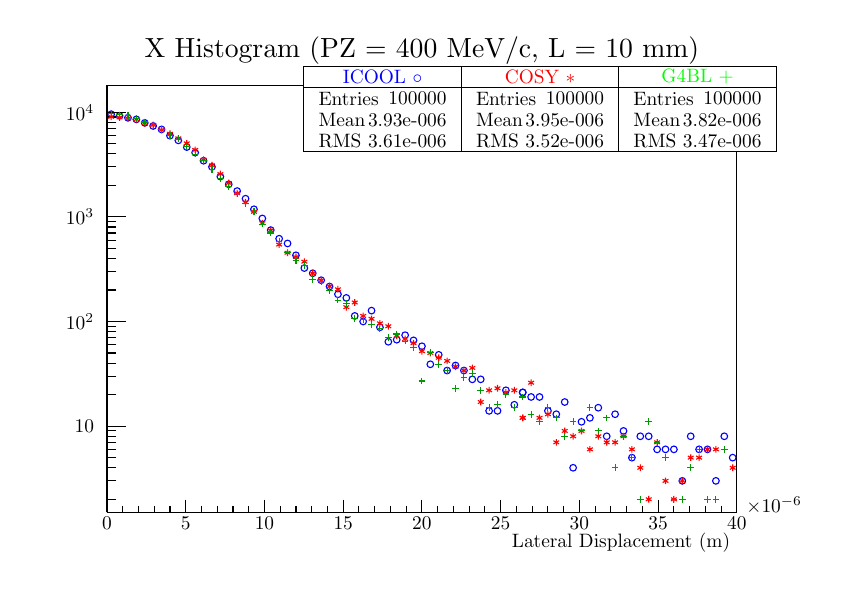
\begin{tikzpicture}
\definecolor{c}{rgb}{1,1,1};
\draw [color=c, fill=c] (0,0) rectangle (20,13.5632);
\draw [color=c, fill=c] (2,1.35632) rectangle (18,12.2069);
\definecolor{c}{rgb}{0,0,0};
\draw [c] (2,1.35632) -- (2,12.2069) -- (18,12.2069) -- (18,1.35632) -- (2,1.35632);
\definecolor{c}{rgb}{1,1,1};
\draw [color=c, fill=c] (2,1.35632) rectangle (18,12.2069);
\definecolor{c}{rgb}{0,0,0};
\draw [c] (2,1.35632) -- (2,12.2069) -- (18,12.2069) -- (18,1.35632) -- (2,1.35632);
\definecolor{c}{rgb}{0,0,1};
\foreach \P in
 {(2.10667,11.4692),(2.32,11.4286),(2.53333,11.3794),(2.74667,11.3377),(2.96,11.2494),(3.17333,11.1705),(3.38667,11.083),(3.6,10.9243),(3.81333,10.8048),(4.02667,10.635),(4.24,10.4937),(4.45333,10.2872),(4.66667,10.1313),(4.88,9.8854),(5.09333,9.6893
1),(5.30667,9.5169),(5.52,9.32346),(5.73333,9.0544),(5.94667,8.82123),(6.16,8.52564),(6.37333,8.3068),(6.58667,8.18683),(6.8,7.88541),(7.01333,7.56137),(7.22667,7.4294),(7.44,7.25279),(7.65333,7.09331),(7.86667,6.8956),(8.08,6.8032),(8.29333,6.34541)
,(8.50667,6.20432),(8.72,6.48024),(8.93333,6.05676),(9.14667,5.68915),(9.36,5.74203),(9.57333,5.85674),(9.78667,5.72467),(10,5.57551),(10.2133,5.11736),(10.4267,5.35705),(10.64,4.95898),(10.8533,5.08738),(11.0667,4.95898),(11.28,4.73485),(11.4933,4.7
3485),(11.7067,3.93471),(11.92,3.93471),(12.1333,4.45646),(12.3467,4.08885),(12.56,4.40276)}{\draw[mark options={color=c,fill=c},mark size=2.402402pt,mark=o] plot coordinates {\P};}
\foreach \P in
 {(12.56,4.40276),(12.7733,4.28723),(12.9867,4.28723),(13.2,3.93471),(13.4133,3.84916),(13.6267,4.15883),(13.84,2.48856),(14.0533,3.65632),(14.2667,3.75676),(14.48,4.01435),(14.6933,3.28871),(14.9067,3.84916),(15.12,3.42467),(15.3333,2.74615),(15.546
7,3.28871),(15.76,3.28871),(15.9733,2.95661),(16.1867,2.95661),(16.4,2.95661),(16.6133,2.15647),(16.8267,3.28871),(17.04,2.95661),(17.2533,2.95661),(17.4667,2.15647),(17.68,3.28871),(17.8933,2.74615)}{\draw[mark options={color=c,fill=c},mark
 size=2.402402pt,mark=o] plot coordinates {\P};}
\definecolor{c}{rgb}{1,1,1};
\draw [color=c, fill=c] (7,10.5115) rectangle (11,12.6816);
\definecolor{c}{rgb}{0,0,0};
\draw [c] (7,10.5115) -- (11,10.5115);
\draw [c] (11,10.5115) -- (11,12.6816);
\draw [c] (11,12.6816) -- (7,12.6816);
\draw [c] (7,12.6816) -- (7,10.5115);
\draw[color=blue](9,12.4103) node[scale=0.7, rotate=0]{ICOOL $\circ$};
\draw [c] (7,12.1391) -- (11,12.1391);
\draw [anchor= west] (7.2,11.8678) node[scale=0.7, rotate=0]{Entries };
\draw [anchor= east] (10.8,11.8678) node[scale=0.7, rotate=0]{ 100000};
\draw [anchor= west] (7.2,11.3253) node[scale=0.7, rotate=0]{Mean  };
\draw [anchor= east] (10.8,11.3253) node[scale=0.7, rotate=0]{ 3.93e-006};
\draw [anchor= west] (7.2,10.7828) node[scale=0.7, rotate=0]{RMS   };
\draw [anchor= east] (10.8,10.7828) node[scale=0.7, rotate=0]{ 3.61e-006};
\draw [c] (2,1.35632) -- (18,1.35632);
\draw [anchor= east] (18,0.596782) node[scale=0.7, rotate=0]{Lateral Displacement (m)};
\draw [c] (2,1.68184) -- (2,1.35632);
\draw [c] (2.4,1.51908) -- (2.4,1.35632);
\draw [c] (2.8,1.51908) -- (2.8,1.35632);
\draw [c] (3.2,1.51908) -- (3.2,1.35632);
\draw [c] (3.6,1.51908) -- (3.6,1.35632);
\draw [c] (4,1.68184) -- (4,1.35632);
\draw [c] (4.4,1.51908) -- (4.4,1.35632);
\draw [c] (4.8,1.51908) -- (4.8,1.35632);
\draw [c] (5.2,1.51908) -- (5.2,1.35632);
\draw [c] (5.6,1.51908) -- (5.6,1.35632);
\draw [c] (6,1.68184) -- (6,1.35632);
\draw [c] (6.4,1.51908) -- (6.4,1.35632);
\draw [c] (6.8,1.51908) -- (6.8,1.35632);
\draw [c] (7.2,1.51908) -- (7.2,1.35632);
\draw [c] (7.6,1.51908) -- (7.6,1.35632);
\draw [c] (8,1.68184) -- (8,1.35632);
\draw [c] (8.4,1.51908) -- (8.4,1.35632);
\draw [c] (8.8,1.51908) -- (8.8,1.35632);
\draw [c] (9.2,1.51908) -- (9.2,1.35632);
\draw [c] (9.6,1.51908) -- (9.6,1.35632);
\draw [c] (10,1.68184) -- (10,1.35632);
\draw [c] (10.4,1.51908) -- (10.4,1.35632);
\draw [c] (10.8,1.51908) -- (10.8,1.35632);
\draw [c] (11.2,1.51908) -- (11.2,1.35632);
\draw [c] (11.6,1.51908) -- (11.6,1.35632);
\draw [c] (12,1.68184) -- (12,1.35632);
\draw [c] (12.4,1.51908) -- (12.4,1.35632);
\draw [c] (12.8,1.51908) -- (12.8,1.35632);
\draw [c] (13.2,1.51908) -- (13.2,1.35632);
\draw [c] (13.6,1.51908) -- (13.6,1.35632);
\draw [c] (14,1.68184) -- (14,1.35632);
\draw [c] (14.4,1.51908) -- (14.4,1.35632);
\draw [c] (14.8,1.51908) -- (14.8,1.35632);
\draw [c] (15.2,1.51908) -- (15.2,1.35632);
\draw [c] (15.6,1.51908) -- (15.6,1.35632);
\draw [c] (16,1.68184) -- (16,1.35632);
\draw [c] (16.4,1.51908) -- (16.4,1.35632);
\draw [c] (16.8,1.51908) -- (16.8,1.35632);
\draw [c] (17.2,1.51908) -- (17.2,1.35632);
\draw [c] (17.6,1.51908) -- (17.6,1.35632);
\draw [c] (18,1.68184) -- (18,1.35632);
\draw [anchor=base] (2,0.908736) node[scale=0.7, rotate=0]{0};
\draw [anchor=base] (4,0.908736) node[scale=0.7, rotate=0]{5};
\draw [anchor=base] (6,0.908736) node[scale=0.7, rotate=0]{10};
\draw [anchor=base] (8,0.908736) node[scale=0.7, rotate=0]{15};
\draw [anchor=base] (10,0.908736) node[scale=0.7, rotate=0]{20};
\draw [anchor=base] (12,0.908736) node[scale=0.7, rotate=0]{25};
\draw [anchor=base] (14,0.908736) node[scale=0.7, rotate=0]{30};
\draw [anchor=base] (16,0.908736) node[scale=0.7, rotate=0]{35};
\draw [anchor=base] (18,0.908736) node[scale=0.7, rotate=0]{40};
\draw [anchor=base west] (18.07,1.35632) node[scale=0.7, rotate=0]{$\times10^{-6}$};
\draw [c] (2,1.35632) -- (2,12.2069);
\draw [c] (2.24,1.68841) -- (2,1.68841);
\draw [c] (2.24,2.15647) -- (2,2.15647);
\draw [c] (2.24,2.48856) -- (2,2.48856);
\draw [c] (2.24,2.74615) -- (2,2.74615);
\draw [c] (2.24,2.95661) -- (2,2.95661);
\draw [c] (2.24,3.13456) -- (2,3.13456);
\draw [c] (2.24,3.2887) -- (2,3.2887);
\draw [c] (2.24,3.42467) -- (2,3.42467);
\draw [c] (2.48,3.54629) -- (2,3.54629);
\draw [anchor= east] (1.844,3.54629) node[scale=0.7, rotate=0]{10};
\draw [c] (2.24,4.34644) -- (2,4.34644);
\draw [c] (2.24,4.8145) -- (2,4.8145);
\draw [c] (2.24,5.14659) -- (2,5.14659);
\draw [c] (2.24,5.40418) -- (2,5.40418);
\draw [c] (2.24,5.61464) -- (2,5.61464);
\draw [c] (2.24,5.79259) -- (2,5.79259);
\draw [c] (2.24,5.94673) -- (2,5.94673);
\draw [c] (2.24,6.0827) -- (2,6.0827);
\draw [c] (2.48,6.20432) -- (2,6.20432);
\draw [anchor= east] (1.844,6.20432) node[scale=0.7, rotate=0]{$10^{2}$};
\draw [c] (2.24,7.00447) -- (2,7.00447);
\draw [c] (2.24,7.47253) -- (2,7.47253);
\draw [c] (2.24,7.80462) -- (2,7.80462);
\draw [c] (2.24,8.06221) -- (2,8.06221);
\draw [c] (2.24,8.27267) -- (2,8.27267);
\draw [c] (2.24,8.45062) -- (2,8.45062);
\draw [c] (2.24,8.60476) -- (2,8.60476);
\draw [c] (2.24,8.74073) -- (2,8.74073);
\draw [c] (2.48,8.86235) -- (2,8.86235);
\draw [anchor= east] (1.844,8.86235) node[scale=0.7, rotate=0]{$10^{3}$};
\draw [c] (2.24,9.6625) -- (2,9.6625);
\draw [c] (2.24,10.1306) -- (2,10.1306);
\draw [c] (2.24,10.4626) -- (2,10.4626);
\draw [c] (2.24,10.7202) -- (2,10.7202);
\draw [c] (2.24,10.9307) -- (2,10.9307);
\draw [c] (2.24,11.1086) -- (2,11.1086);
\draw [c] (2.24,11.2628) -- (2,11.2628);
\draw [c] (2.24,11.3988) -- (2,11.3988);
\draw [c] (2.48,11.5204) -- (2,11.5204);
\draw [anchor= east] (1.844,11.5204) node[scale=0.7, rotate=0]{$10^{4}$};
\definecolor{c}{rgb}{1,1,1};
\draw [color=c, fill=c] (7,10.5115) rectangle (11,12.6816);
\definecolor{c}{rgb}{0,0,0};
\draw [c] (7,10.5115) -- (11,10.5115);
\draw [c] (11,10.5115) -- (11,12.6816);
\draw [c] (11,12.6816) -- (7,12.6816);
\draw [c] (7,12.6816) -- (7,10.5115);
\draw[color=blue](9,12.4103) node[scale=0.7, rotate=0]{ICOOL $\circ$};
\draw [c] (7,12.1391) -- (11,12.1391);
\draw [anchor= west] (7.2,11.8678) node[scale=0.7, rotate=0]{Entries };
\draw [anchor= east] (10.8,11.8678) node[scale=0.7, rotate=0]{ 100000};
\draw [anchor= west] (7.2,11.3253) node[scale=0.7, rotate=0]{Mean  };
\draw [anchor= east] (10.8,11.3253) node[scale=0.7, rotate=0]{ 3.93e-006};
\draw [anchor= west] (7.2,10.7828) node[scale=0.7, rotate=0]{RMS   };
\draw [anchor= east] (10.8,10.7828) node[scale=0.7, rotate=0]{ 3.61e-006};
\draw (10,13.0816) node[scale=1, rotate=0]{X Histogram (PZ = 400 MeV/c, L = 10 mm)};
\definecolor{c}{rgb}{1,0,0};
\foreach \P in
 {(2.10667,11.4029),(2.32,11.3851),(2.53333,11.366),(2.74667,11.341),(2.96,11.2398),(3.17333,11.1957),(3.38667,11.0709),(3.6,10.9728),(3.81333,10.856),(4.02667,10.729),(4.24,10.5624),(4.45333,10.3115),(4.66667,10.171),(4.88,9.94927),(5.09333,9.72212)
,(5.30667,9.46329),(5.52,9.23499),(5.73333,8.99008),(5.94667,8.70159),(6.16,8.51944),(6.37333,8.15744),(6.58667,7.9508),(6.8,7.84154),(7.01333,7.72394),(7.22667,7.4294),(7.44,7.25279),(7.65333,7.09864),(7.86667,7.02166),(8.08,6.56773),(8.29333,6.6876
7),(8.50667,6.34541),(8.72,6.27159),(8.93333,6.1572),(9.14667,6.0827),(9.36,5.84103),(9.57333,5.75913),(9.78667,5.6525),(10,5.44945),(10.2133,5.40418),(10.4267,5.28255),(10.64,5.20291),(10.8533,5.05659),(11.0667,4.95898),(11.28,5.02496),(11.4933,4.15
883),(11.7067,4.45646),(11.92,4.50778),(12.1333,4.40276),(12.3467,4.45646),(12.56,3.75676)}{\draw[mark options={color=c,fill=c},mark size=2.402402pt,mark=asterisk] plot coordinates {\P};}
\foreach \P in
 {(12.56,3.75676),(12.7733,4.64931),(12.9867,3.75676),(13.2,3.84916),(13.4133,3.13456),(13.6267,3.42467),(13.84,3.28871),(14.0533,3.42467),(14.2667,2.95661),(14.48,3.28871),(14.6933,3.13456),(14.9067,3.13456),(15.12,3.28871),(15.3333,2.95661),(15.546
7,2.48856),(15.76,1.68841),(15.9733,3.13456),(16.1867,2.15647),(16.4,1.68841),(16.6133,2.15647),(16.8267,2.74615),(17.04,2.74615),(17.2533,2.95661),(17.4667,2.95661),(17.8933,2.48856)}{\draw[mark options={color=c,fill=c},mark
 size=2.402402pt,mark=asterisk] plot coordinates {\P};}
\definecolor{c}{rgb}{1,1,1};
\draw [color=c, fill=c] (11,10.5115) rectangle (15,12.6816);
\definecolor{c}{rgb}{0,0,0};
\draw [c] (11,10.5115) -- (15,10.5115);
\draw [c] (15,10.5115) -- (15,12.6816);
\draw [c] (15,12.6816) -- (11,12.6816);
\draw [c] (11,12.6816) -- (11,10.5115);
\draw [color=red](13,12.4103) node[scale=0.7, rotate=0]{COSY $*$};
\draw [c] (11,12.1391) -- (15,12.1391);
\draw [anchor= west] (11.2,11.8678) node[scale=0.7, rotate=0]{Entries };
\draw [anchor= east] (14.8,11.8678) node[scale=0.7, rotate=0]{ 100000};
\draw [anchor= west] (11.2,11.3253) node[scale=0.7, rotate=0]{Mean  };
\draw [anchor= east] (14.8,11.3253) node[scale=0.7, rotate=0]{ 3.95e-006};
\draw [anchor= west] (11.2,10.7828) node[scale=0.7, rotate=0]{RMS   };
\draw [anchor= east] (14.8,10.7828) node[scale=0.7, rotate=0]{ 3.52e-006};
\definecolor{c}{rgb}{1,1,1};
\draw [color=c, fill=c] (11,10.5115) rectangle (15,12.6816);
\definecolor{c}{rgb}{0,0,0};
\draw [c] (11,10.5115) -- (15,10.5115);
\draw [c] (15,10.5115) -- (15,12.6816);
\draw [c] (15,12.6816) -- (11,12.6816);
\draw [c] (11,12.6816) -- (11,10.5115);
\draw [color=red](13,12.4103) node[scale=0.7, rotate=0]{COSY $*$};
\draw [c] (11,12.1391) -- (15,12.1391);
\draw [anchor= west] (11.2,11.8678) node[scale=0.7, rotate=0]{Entries };
\draw [anchor= east] (14.8,11.8678) node[scale=0.7, rotate=0]{ 100000};
\draw [anchor= west] (11.2,11.3253) node[scale=0.7, rotate=0]{Mean  };
\draw [anchor= east] (14.8,11.3253) node[scale=0.7, rotate=0]{ 3.95e-006};
\draw [anchor= west] (11.2,10.7828) node[scale=0.7, rotate=0]{RMS   };
\draw [anchor= east] (14.8,10.7828) node[scale=0.7, rotate=0]{ 3.52e-006};
\definecolor{c}{rgb}{0,0.6,0};
\foreach \P in
 {(2.10667,11.4967),(2.32,11.4528),(2.53333,11.4286),(2.74667,11.3636),(2.96,11.2708),(3.17333,11.1751),(3.38667,11.0858),(3.6,10.9363),(3.81333,10.8357),(4.02667,10.6407),(4.24,10.4542),(4.45333,10.2996),(4.66667,10.0705),(4.88,9.83184),(5.09333,9.6
3859),(5.30667,9.44392),(5.52,9.19242),(5.73333,8.99111),(5.94667,8.67881),(6.16,8.45062),(6.37333,8.24739),(6.58667,7.9457),(6.8,7.75749),(7.01333,7.63051),(7.22667,7.26667),(7.44,7.22452),(7.65333,6.98702),(7.86667,6.74688),(8.08,6.65688),(8.29333,
6.28243),(8.50667,6.2496),(8.72,6.1329),(8.93333,6.01672),(9.14667,5.79259),(9.36,5.88752),(9.57333,5.70704),(9.78667,5.535),(10,4.69287),(10.2133,5.42704),(10.4267,5.11736),(10.64,4.95898),(10.8533,4.50778),(11.0667,4.77536),(11.28,4.889),(11.4933,4
.45646),(11.7067,4.01435),(11.92,4.08885),(12.1333,4.34644),(12.3467,4.01435),(12.56,4.28723)}{\draw[mark options={color=c,fill=c},mark size=2.402402pt,mark=+] plot coordinates {\P};}
\foreach \P in
 {(12.56,4.28723),(12.7733,3.84916),(12.9867,3.65632),(13.2,4.01435),(13.4133,3.75676),(13.6267,3.28871),(13.84,3.65632),(14.0533,3.42467),(14.2667,4.01435),(14.48,3.42467),(14.6933,3.75676),(14.9067,2.48856),(15.12,3.28871),(15.3333,2.74615),(15.546
7,1.68841),(15.76,3.65632),(15.9733,3.13456),(16.1867,2.74615),(16.4,1.68841),(16.6133,1.68841),(16.8267,2.48856),(17.04,2.95661),(17.2533,1.68841),(17.4667,1.68841),(17.68,2.95661)}{\draw[mark options={color=c,fill=c},mark size=2.402402pt,mark=+]
 plot coordinates {\P};}
\definecolor{c}{rgb}{1,1,1};
\draw [color=c, fill=c] (15,10.5115) rectangle (19,12.6816);
\definecolor{c}{rgb}{0,0,0};
\draw [c] (15,10.5115) -- (19,10.5115);
\draw [c] (19,10.5115) -- (19,12.6816);
\draw [c] (19,12.6816) -- (15,12.6816);
\draw [c] (15,12.6816) -- (15,10.5115);
\draw [color=green](17,12.4103) node[scale=0.7, rotate=0]{G4BL $+$};
\draw [c] (15,12.1391) -- (19,12.1391);
\draw [anchor= west] (15.2,11.8678) node[scale=0.7, rotate=0]{Entries };
\draw [anchor= east] (18.8,11.8678) node[scale=0.7, rotate=0]{ 100000};
\draw [anchor= west] (15.2,11.3253) node[scale=0.7, rotate=0]{Mean  };
\draw [anchor= east] (18.8,11.3253) node[scale=0.7, rotate=0]{ 3.82e-006};
\draw [anchor= west] (15.2,10.7828) node[scale=0.7, rotate=0]{RMS   };
\draw [anchor= east] (18.8,10.7828) node[scale=0.7, rotate=0]{ 3.47e-006};
\definecolor{c}{rgb}{1,1,1};
\draw [color=c, fill=c] (15,10.5115) rectangle (19,12.6816);
\definecolor{c}{rgb}{0,0,0};
\draw [c] (15,10.5115) -- (19,10.5115);
\draw [c] (19,10.5115) -- (19,12.6816);
\draw [c] (19,12.6816) -- (15,12.6816);
\draw [c] (15,12.6816) -- (15,10.5115);
\draw [color=green](17,12.4103) node[scale=0.7, rotate=0]{G4BL $+$};
\draw [c] (15,12.1391) -- (19,12.1391);
\draw [anchor= west] (15.2,11.8678) node[scale=0.7, rotate=0]{Entries };
\draw [anchor= east] (18.8,11.8678) node[scale=0.7, rotate=0]{ 100000};
\draw [anchor= west] (15.2,11.3253) node[scale=0.7, rotate=0]{Mean  };
\draw [anchor= east] (18.8,11.3253) node[scale=0.7, rotate=0]{ 3.82e-006};
\draw [anchor= west] (15.2,10.7828) node[scale=0.7, rotate=0]{RMS   };
\draw [anchor= east] (18.8,10.7828) node[scale=0.7, rotate=0]{ 3.47e-006};
\end{tikzpicture}
}\\
\frame{    \pgfdeclareplotmark{cross} {
\pgfpathmoveto{\pgfpoint{-0.3\pgfplotmarksize}{\pgfplotmarksize}}
\pgfpathlineto{\pgfpoint{+0.3\pgfplotmarksize}{\pgfplotmarksize}}
\pgfpathlineto{\pgfpoint{+0.3\pgfplotmarksize}{0.3\pgfplotmarksize}}
\pgfpathlineto{\pgfpoint{+1\pgfplotmarksize}{0.3\pgfplotmarksize}}
\pgfpathlineto{\pgfpoint{+1\pgfplotmarksize}{-0.3\pgfplotmarksize}}
\pgfpathlineto{\pgfpoint{+0.3\pgfplotmarksize}{-0.3\pgfplotmarksize}}
\pgfpathlineto{\pgfpoint{+0.3\pgfplotmarksize}{-1.\pgfplotmarksize}}
\pgfpathlineto{\pgfpoint{-0.3\pgfplotmarksize}{-1.\pgfplotmarksize}}
\pgfpathlineto{\pgfpoint{-0.3\pgfplotmarksize}{-0.3\pgfplotmarksize}}
\pgfpathlineto{\pgfpoint{-1.\pgfplotmarksize}{-0.3\pgfplotmarksize}}
\pgfpathlineto{\pgfpoint{-1.\pgfplotmarksize}{0.3\pgfplotmarksize}}
\pgfpathlineto{\pgfpoint{-0.3\pgfplotmarksize}{0.3\pgfplotmarksize}}
\pgfpathclose
\pgfusepathqstroke
}
\pgfdeclareplotmark{cross*} {
\pgfpathmoveto{\pgfpoint{-0.3\pgfplotmarksize}{\pgfplotmarksize}}
\pgfpathlineto{\pgfpoint{+0.3\pgfplotmarksize}{\pgfplotmarksize}}
\pgfpathlineto{\pgfpoint{+0.3\pgfplotmarksize}{0.3\pgfplotmarksize}}
\pgfpathlineto{\pgfpoint{+1\pgfplotmarksize}{0.3\pgfplotmarksize}}
\pgfpathlineto{\pgfpoint{+1\pgfplotmarksize}{-0.3\pgfplotmarksize}}
\pgfpathlineto{\pgfpoint{+0.3\pgfplotmarksize}{-0.3\pgfplotmarksize}}
\pgfpathlineto{\pgfpoint{+0.3\pgfplotmarksize}{-1.\pgfplotmarksize}}
\pgfpathlineto{\pgfpoint{-0.3\pgfplotmarksize}{-1.\pgfplotmarksize}}
\pgfpathlineto{\pgfpoint{-0.3\pgfplotmarksize}{-0.3\pgfplotmarksize}}
\pgfpathlineto{\pgfpoint{-1.\pgfplotmarksize}{-0.3\pgfplotmarksize}}
\pgfpathlineto{\pgfpoint{-1.\pgfplotmarksize}{0.3\pgfplotmarksize}}
\pgfpathlineto{\pgfpoint{-0.3\pgfplotmarksize}{0.3\pgfplotmarksize}}
\pgfpathclose
\pgfusepathqfillstroke
}
\pgfdeclareplotmark{newstar} {
\pgfpathmoveto{\pgfqpoint{0pt}{\pgfplotmarksize}}
\pgfpathlineto{\pgfqpointpolar{44}{0.5\pgfplotmarksize}}
\pgfpathlineto{\pgfqpointpolar{18}{\pgfplotmarksize}}
\pgfpathlineto{\pgfqpointpolar{-20}{0.5\pgfplotmarksize}}
\pgfpathlineto{\pgfqpointpolar{-54}{\pgfplotmarksize}}
\pgfpathlineto{\pgfqpointpolar{-90}{0.5\pgfplotmarksize}}
\pgfpathlineto{\pgfqpointpolar{234}{\pgfplotmarksize}}
\pgfpathlineto{\pgfqpointpolar{198}{0.5\pgfplotmarksize}}
\pgfpathlineto{\pgfqpointpolar{162}{\pgfplotmarksize}}
\pgfpathlineto{\pgfqpointpolar{134}{0.5\pgfplotmarksize}}
\pgfpathclose
\pgfusepathqstroke
}
\pgfdeclareplotmark{newstar*} {
\pgfpathmoveto{\pgfqpoint{0pt}{\pgfplotmarksize}}
\pgfpathlineto{\pgfqpointpolar{44}{0.5\pgfplotmarksize}}
\pgfpathlineto{\pgfqpointpolar{18}{\pgfplotmarksize}}
\pgfpathlineto{\pgfqpointpolar{-20}{0.5\pgfplotmarksize}}
\pgfpathlineto{\pgfqpointpolar{-54}{\pgfplotmarksize}}
\pgfpathlineto{\pgfqpointpolar{-90}{0.5\pgfplotmarksize}}
\pgfpathlineto{\pgfqpointpolar{234}{\pgfplotmarksize}}
\pgfpathlineto{\pgfqpointpolar{198}{0.5\pgfplotmarksize}}
\pgfpathlineto{\pgfqpointpolar{162}{\pgfplotmarksize}}
\pgfpathlineto{\pgfqpointpolar{134}{0.5\pgfplotmarksize}}
\pgfpathclose
\pgfusepathqfillstroke
}
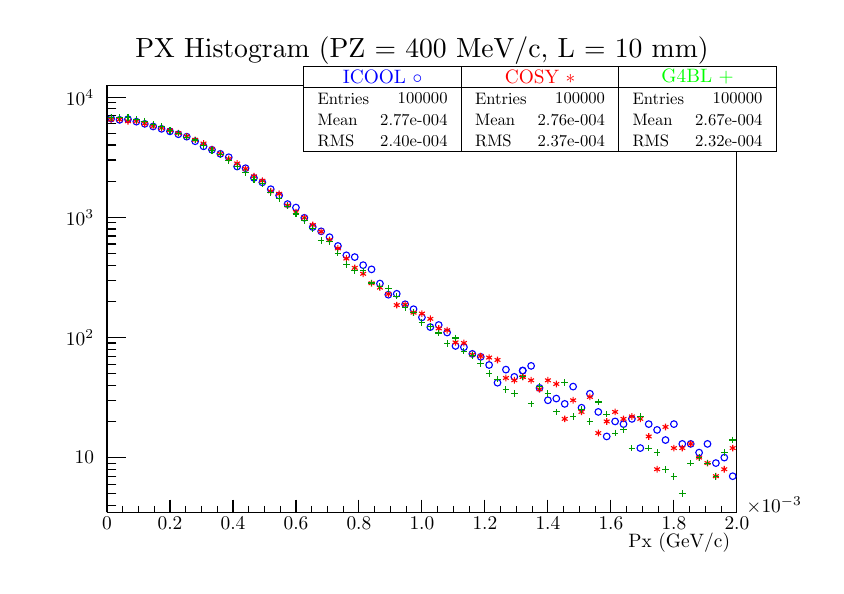
\begin{tikzpicture}
\definecolor{c}{rgb}{1,1,1};
\draw [color=c, fill=c] (0,0) rectangle (20,13.5632);
\draw [color=c, fill=c] (2,1.35632) rectangle (18,12.2069);
\definecolor{c}{rgb}{0,0,0};
\draw [c] (2,1.35632) -- (2,12.2069) -- (18,12.2069) -- (18,1.35632) -- (2,1.35632);
\definecolor{c}{rgb}{1,1,1};
\draw [color=c, fill=c] (2,1.35632) rectangle (18,12.2069);
\definecolor{c}{rgb}{0,0,0};
\draw [c] (2,1.35632) -- (2,12.2069) -- (18,12.2069) -- (18,1.35632) -- (2,1.35632);
\definecolor{c}{rgb}{0,0,1};
\foreach \P in
 {(2.10667,11.3601),(2.32,11.3256),(2.53333,11.3418),(2.74667,11.28),(2.96,11.2245),(3.17333,11.1577),(3.38667,11.0977),(3.6,11.0337),(3.81333,10.9606),(4.02667,10.8986),(4.24,10.7828),(4.45333,10.6535),(4.66667,10.5665),(4.88,10.4628),(5.09333,10.37
65),(5.30667,10.1403),(5.52,10.0976),(5.73333,9.85071),(5.94667,9.73841),(6.16,9.56496),(6.37333,9.40512),(6.58667,9.18685),(6.8,9.09763),(7.01333,8.83746),(7.22667,8.60254),(7.44,8.49448),(7.65333,8.34619),(7.86667,8.12307),(8.08,7.88515),(8.29333,7
.84051),(8.50667,7.63531),(8.72,7.52842),(8.93333,7.16742),(9.14667,6.88465),(9.36,6.9078),(9.57333,6.6419),(9.78667,6.51701),(10,6.3089),(10.2133,6.0619),(10.4267,6.11512),(10.64,5.9247),(10.8533,5.58307),(11.0667,5.55151),(11.28,5.3814),(11.4933,5.
30673),(11.7067,5.09927),(11.92,4.64893),(12.1333,4.98194),(12.3467,4.79797),(12.56,4.95717)}{\draw[mark options={color=c,fill=c},mark size=2.402402pt,mark=o] plot coordinates {\P};}
\foreach \P in
 {(12.56,4.95717),(12.7733,5.07662),(12.9867,4.51632),(13.2,4.20309),(13.4133,4.24654),(13.6267,4.11167),(13.84,4.55074),(14.0533,4.01348),(14.2667,4.36894),(14.48,3.90742),(14.6933,3.28464),(14.9067,3.66583),(15.12,3.59787),(15.3333,3.73048),(15.546
7,2.98897),(15.76,3.59787),(15.9733,3.45049),(16.1867,3.19322),(16.4,3.59787),(16.6133,3.09503),(16.8267,3.09503),(17.04,2.87367),(17.2533,3.09503),(17.4667,2.60778),(17.68,2.74738),(17.8933,2.27477)}{\draw[mark options={color=c,fill=c},mark
 size=2.402402pt,mark=o] plot coordinates {\P};}
\definecolor{c}{rgb}{1,1,1};
\draw [color=c, fill=c] (7,10.5115) rectangle (11,12.6816);
\definecolor{c}{rgb}{0,0,0};
\draw [c] (7,10.5115) -- (11,10.5115);
\draw [c] (11,10.5115) -- (11,12.6816);
\draw [c] (11,12.6816) -- (7,12.6816);
\draw [c] (7,12.6816) -- (7,10.5115);
\draw[color=blue](9,12.4103) node[scale=0.7, rotate=0]{ICOOL $\circ$};
\draw [c] (7,12.1391) -- (11,12.1391);
\draw [anchor= west] (7.2,11.8678) node[scale=0.6, rotate=0]{Entries };
\draw [anchor= east] (10.8,11.8678) node[scale=0.6, rotate=0]{ 100000};
\draw [anchor= west] (7.2,11.3253) node[scale=0.6, rotate=0]{Mean  };
\draw [anchor= east] (10.8,11.3253) node[scale=0.6, rotate=0]{ 2.77e-004};
\draw [anchor= west] (7.2,10.7828) node[scale=0.6, rotate=0]{RMS   };
\draw [anchor= east] (10.8,10.7828) node[scale=0.6, rotate=0]{ 2.40e-004};
\draw [c] (2,1.35632) -- (18,1.35632);
\draw [anchor= east] (18,0.596782) node[scale=0.7, rotate=0]{Px (GeV/c)};
\draw [c] (2,1.68184) -- (2,1.35632);
\draw [c] (2.4,1.51908) -- (2.4,1.35632);
\draw [c] (2.8,1.51908) -- (2.8,1.35632);
\draw [c] (3.2,1.51908) -- (3.2,1.35632);
\draw [c] (3.6,1.68184) -- (3.6,1.35632);
\draw [c] (4,1.51908) -- (4,1.35632);
\draw [c] (4.4,1.51908) -- (4.4,1.35632);
\draw [c] (4.8,1.51908) -- (4.8,1.35632);
\draw [c] (5.2,1.68184) -- (5.2,1.35632);
\draw [c] (5.6,1.51908) -- (5.6,1.35632);
\draw [c] (6,1.51908) -- (6,1.35632);
\draw [c] (6.4,1.51908) -- (6.4,1.35632);
\draw [c] (6.8,1.68184) -- (6.8,1.35632);
\draw [c] (7.2,1.51908) -- (7.2,1.35632);
\draw [c] (7.6,1.51908) -- (7.6,1.35632);
\draw [c] (8,1.51908) -- (8,1.35632);
\draw [c] (8.4,1.68184) -- (8.4,1.35632);
\draw [c] (8.8,1.51908) -- (8.8,1.35632);
\draw [c] (9.2,1.51908) -- (9.2,1.35632);
\draw [c] (9.6,1.51908) -- (9.6,1.35632);
\draw [c] (10,1.68184) -- (10,1.35632);
\draw [c] (10.4,1.51908) -- (10.4,1.35632);
\draw [c] (10.8,1.51908) -- (10.8,1.35632);
\draw [c] (11.2,1.51908) -- (11.2,1.35632);
\draw [c] (11.6,1.68184) -- (11.6,1.35632);
\draw [c] (12,1.51908) -- (12,1.35632);
\draw [c] (12.4,1.51908) -- (12.4,1.35632);
\draw [c] (12.8,1.51908) -- (12.8,1.35632);
\draw [c] (13.2,1.68184) -- (13.2,1.35632);
\draw [c] (13.6,1.51908) -- (13.6,1.35632);
\draw [c] (14,1.51908) -- (14,1.35632);
\draw [c] (14.4,1.51908) -- (14.4,1.35632);
\draw [c] (14.8,1.68184) -- (14.8,1.35632);
\draw [c] (15.2,1.51908) -- (15.2,1.35632);
\draw [c] (15.6,1.51908) -- (15.6,1.35632);
\draw [c] (16,1.51908) -- (16,1.35632);
\draw [c] (16.4,1.68184) -- (16.4,1.35632);
\draw [c] (16.8,1.51908) -- (16.8,1.35632);
\draw [c] (17.2,1.51908) -- (17.2,1.35632);
\draw [c] (17.6,1.51908) -- (17.6,1.35632);
\draw [c] (18,1.68184) -- (18,1.35632);
\draw [anchor=base] (2,0.908736) node[scale=0.7, rotate=0]{0};
\draw [anchor=base] (3.6,0.908736) node[scale=0.7, rotate=0]{0.2};
\draw [anchor=base] (5.2,0.908736) node[scale=0.7, rotate=0]{0.4};
\draw [anchor=base] (6.8,0.908736) node[scale=0.7, rotate=0]{0.6};
\draw [anchor=base] (8.4,0.908736) node[scale=0.7, rotate=0]{0.8};
\draw [anchor=base] (10,0.908736) node[scale=0.7, rotate=0]{1.0};
\draw [anchor=base] (11.6,0.908736) node[scale=0.7, rotate=0]{1.2};
\draw [anchor=base] (13.2,0.908736) node[scale=0.7, rotate=0]{1.4};
\draw [anchor=base] (14.8,0.908736) node[scale=0.7, rotate=0]{1.6};
\draw [anchor=base] (16.4,0.908736) node[scale=0.7, rotate=0]{1.8};
\draw [anchor=base] (18,0.908736) node[scale=0.7, rotate=0]{2.0};
\draw [anchor=base west] (18.07,1.35632) node[scale=0.7, rotate=0]{$\times10^{-3}$};
\draw [c] (2,1.35632) -- (2,12.2069);
\draw [c] (2.24,1.53325) -- (2,1.53325);
\draw [c] (2.24,1.82893) -- (2,1.82893);
\draw [c] (2.24,2.07051) -- (2,2.07051);
\draw [c] (2.24,2.27477) -- (2,2.27477);
\draw [c] (2.24,2.4517) -- (2,2.4517);
\draw [c] (2.24,2.60777) -- (2,2.60777);
\draw [c] (2.48,2.74738) -- (2,2.74738);
\draw [anchor= east] (1.844,2.74738) node[scale=0.7, rotate=0]{10};
\draw [c] (2.24,3.66583) -- (2,3.66583);
\draw [c] (2.24,4.20309) -- (2,4.20309);
\draw [c] (2.24,4.58428) -- (2,4.58428);
\draw [c] (2.24,4.87996) -- (2,4.87996);
\draw [c] (2.24,5.12154) -- (2,5.12154);
\draw [c] (2.24,5.3258) -- (2,5.3258);
\draw [c] (2.24,5.50273) -- (2,5.50273);
\draw [c] (2.24,5.6588) -- (2,5.6588);
\draw [c] (2.48,5.79841) -- (2,5.79841);
\draw [anchor= east] (1.844,5.79841) node[scale=0.7, rotate=0]{$10^{2}$};
\draw [c] (2.24,6.71686) -- (2,6.71686);
\draw [c] (2.24,7.25412) -- (2,7.25412);
\draw [c] (2.24,7.63531) -- (2,7.63531);
\draw [c] (2.24,7.93098) -- (2,7.93098);
\draw [c] (2.24,8.17257) -- (2,8.17257);
\draw [c] (2.24,8.37683) -- (2,8.37683);
\draw [c] (2.24,8.55376) -- (2,8.55376);
\draw [c] (2.24,8.70983) -- (2,8.70983);
\draw [c] (2.48,8.84944) -- (2,8.84944);
\draw [anchor= east] (1.844,8.84944) node[scale=0.7, rotate=0]{$10^{3}$};
\draw [c] (2.24,9.76789) -- (2,9.76789);
\draw [c] (2.24,10.3051) -- (2,10.3051);
\draw [c] (2.24,10.6863) -- (2,10.6863);
\draw [c] (2.24,10.982) -- (2,10.982);
\draw [c] (2.24,11.2236) -- (2,11.2236);
\draw [c] (2.24,11.4279) -- (2,11.4279);
\draw [c] (2.24,11.6048) -- (2,11.6048);
\draw [c] (2.24,11.7609) -- (2,11.7609);
\draw [c] (2.48,11.9005) -- (2,11.9005);
\draw [anchor= east] (1.844,11.9005) node[scale=0.7, rotate=0]{$10^{4}$};
\definecolor{c}{rgb}{1,1,1};
\draw [color=c, fill=c] (7,10.5115) rectangle (11,12.6816);
\definecolor{c}{rgb}{0,0,0};
\draw [c] (7,10.5115) -- (11,10.5115);
\draw [c] (11,10.5115) -- (11,12.6816);
\draw [c] (11,12.6816) -- (7,12.6816);
\draw [c] (7,12.6816) -- (7,10.5115);
\draw[color=blue](9,12.4103) node[scale=0.7, rotate=0]{ICOOL $\circ$};
\draw [c] (7,12.1391) -- (11,12.1391);
\draw [anchor= west] (7.2,11.8678) node[scale=0.6, rotate=0]{Entries };
\draw [anchor= east] (10.8,11.8678) node[scale=0.6, rotate=0]{ 100000};
\draw [anchor= west] (7.2,11.3253) node[scale=0.6, rotate=0]{Mean  };
\draw [anchor= east] (10.8,11.3253) node[scale=0.6, rotate=0]{ 2.77e-004};
\draw [anchor= west] (7.2,10.7828) node[scale=0.6, rotate=0]{RMS   };
\draw [anchor= east] (10.8,10.7828) node[scale=0.6, rotate=0]{ 2.40e-004};
\draw (10,13.0816) node[scale=1, rotate=0]{PX Histogram (PZ = 400 MeV/c, L = 10 mm)};
\definecolor{c}{rgb}{1,0,0};
\foreach \P in
 {(2.10667,11.3337),(2.32,11.3339),(2.53333,11.2918),(2.74667,11.2927),(2.96,11.2302),(3.17333,11.1658),(3.38667,11.1191),(3.6,11.0592),(3.81333,10.9876),(4.02667,10.9065),(4.24,10.8183),(4.45333,10.7252),(4.66667,10.5827),(4.88,10.4636),(5.09333,10.
334),(5.30667,10.2189),(5.52,10.0804),(5.73333,9.89177),(5.94667,9.78173),(6.16,9.51057),(6.37333,9.44798),(6.58667,9.1504),(6.8,8.98174),(7.01333,8.84013),(7.22667,8.65727),(7.44,8.48754),(7.65333,8.27659),(7.86667,8.06209),(8.08,7.8031),(8.29333,7.
56735),(8.50667,7.41606),(8.72,7.17682),(8.93333,7.0645),(9.14667,6.90205),(9.36,6.6207),(9.57333,6.63487),(9.78667,6.42944),(10,6.40452),(10.2133,6.27234),(10.4267,6.02891),(10.64,5.9836),(10.8533,5.67344),(11.0667,5.6588),(11.28,5.36313),(11.4933,5
.3258),(11.7067,5.28739),(11.92,5.2276),(12.1333,4.76947),(12.3467,4.71057),(12.56,4.79797)}{\draw[mark options={color=c,fill=c},mark size=2.402402pt,mark=asterisk] plot coordinates {\P};}
\foreach \P in
 {(12.56,4.79797),(12.7733,4.71057),(12.9867,4.48098),(13.2,4.71057),(13.4133,4.617),(13.6267,3.73048),(13.84,4.20309),(14.0533,3.90742),(14.2667,4.28861),(14.48,3.37016),(14.6933,3.66583),(14.9067,3.90742),(15.12,3.73048),(15.3333,3.79212),(15.5467,
3.73048),(15.76,3.28464),(15.9733,2.45171),(16.1867,3.52623),(16.4,2.98897),(16.6133,2.98897),(16.8267,3.09503),(17.04,2.74738),(17.2533,2.60778),(17.4667,2.27477),(17.68,2.45171),(17.8933,2.98897)}{\draw[mark options={color=c,fill=c},mark
 size=2.402402pt,mark=asterisk] plot coordinates {\P};}
\definecolor{c}{rgb}{1,1,1};
\draw [color=c, fill=c] (11,10.5115) rectangle (15,12.6816);
\definecolor{c}{rgb}{0,0,0};
\draw [c] (11,10.5115) -- (15,10.5115);
\draw [c] (15,10.5115) -- (15,12.6816);
\draw [c] (15,12.6816) -- (11,12.6816);
\draw [c] (11,12.6816) -- (11,10.5115);
\draw [color=red](13,12.4103) node[scale=0.7, rotate=0]{COSY $*$};
\draw [c] (11,12.1391) -- (15,12.1391);
\draw [anchor= west] (11.2,11.8678) node[scale=0.6, rotate=0]{Entries };
\draw [anchor= east] (14.8,11.8678) node[scale=0.6, rotate=0]{ 100000};
\draw [anchor= west] (11.2,11.3253) node[scale=0.6, rotate=0]{Mean  };
\draw [anchor= east] (14.8,11.3253) node[scale=0.6, rotate=0]{ 2.76e-004};
\draw [anchor= west] (11.2,10.7828) node[scale=0.6, rotate=0]{RMS   };
\draw [anchor= east] (14.8,10.7828) node[scale=0.6, rotate=0]{ 2.37e-004};
\definecolor{c}{rgb}{1,1,1};
\draw [color=c, fill=c] (11,10.5115) rectangle (15,12.6816);
\definecolor{c}{rgb}{0,0,0};
\draw [c] (11,10.5115) -- (15,10.5115);
\draw [c] (15,10.5115) -- (15,12.6816);
\draw [c] (15,12.6816) -- (11,12.6816);
\draw [c] (11,12.6816) -- (11,10.5115);
\draw [color=red](13,12.4103) node[scale=0.7, rotate=0]{COSY $*$};
\draw [c] (11,12.1391) -- (15,12.1391);
\draw [anchor= west] (11.2,11.8678) node[scale=0.6, rotate=0]{Entries };
\draw [anchor= east] (14.8,11.8678) node[scale=0.6, rotate=0]{ 100000};
\draw [anchor= west] (11.2,11.3253) node[scale=0.6, rotate=0]{Mean  };
\draw [anchor= east] (14.8,11.3253) node[scale=0.6, rotate=0]{ 2.76e-004};
\draw [anchor= west] (11.2,10.7828) node[scale=0.6, rotate=0]{RMS   };
\draw [anchor= east] (14.8,10.7828) node[scale=0.6, rotate=0]{ 2.37e-004};
\definecolor{c}{rgb}{0,0.6,0};
\foreach \P in
 {(2.10667,11.3838),(2.32,11.3898),(2.53333,11.3912),(2.74667,11.3299),(2.96,11.2935),(3.17333,11.2074),(3.38667,11.1552),(3.6,11.0484),(3.81333,10.9897),(4.02667,10.8884),(4.24,10.8144),(4.45333,10.673),(4.66667,10.5544),(4.88,10.4529),(5.09333,10.2
896),(5.30667,10.1388),(5.52,9.98101),(5.73333,9.80834),(5.94667,9.70896),(6.16,9.48293),(6.37333,9.33628),(6.58667,9.13554),(6.8,8.93412),(7.01333,8.76745),(7.22667,8.56202),(7.44,8.25809),(7.65333,8.22666),(7.86667,7.94154),(8.08,7.64521),(8.29333,
7.49202),(8.50667,7.48832),(8.72,7.1815),(8.93333,7.09971),(9.14667,7.04396),(9.36,6.84916),(9.57333,6.55498),(9.78667,6.43765),(10,6.18621),(10.2133,6.07271),(10.4267,5.9126),(10.64,5.644),(10.8533,5.78509),(11.0667,5.45209),(11.28,5.34459),(11.4933
,5.14345),(11.7067,4.87996),(11.92,4.74035),(12.1333,4.48098),(12.3467,4.36894),(12.56,4.79797)}{\draw[mark options={color=c,fill=c},mark size=2.402402pt,mark=+] plot coordinates {\P};}
\foreach \P in
 {(12.56,4.79797),(12.7733,4.11167),(12.9867,4.55074),(13.2,4.36894),(13.4133,3.90742),(13.6267,4.64893),(13.84,3.79212),(14.0533,3.96151),(14.2667,3.66583),(14.48,4.15817),(14.6933,3.85102),(14.9067,3.37016),(15.12,3.45049),(15.3333,2.98897),(15.546
7,3.79212),(15.76,2.98897),(15.9733,2.87367),(16.1867,2.45171),(16.4,2.27477),(16.6133,1.82893),(16.8267,2.60778),(17.04,2.74738),(17.2533,2.60778),(17.4667,2.27477),(17.68,2.87367),(17.8933,3.19322)}{\draw[mark options={color=c,fill=c},mark
 size=2.402402pt,mark=+] plot coordinates {\P};}
\definecolor{c}{rgb}{1,1,1};
\draw [color=c, fill=c] (15,10.5115) rectangle (19,12.6816);
\definecolor{c}{rgb}{0,0,0};
\draw [c] (15,10.5115) -- (19,10.5115);
\draw [c] (19,10.5115) -- (19,12.6816);
\draw [c] (19,12.6816) -- (15,12.6816);
\draw [c] (15,12.6816) -- (15,10.5115);
\draw [color=green](17,12.4103) node[scale=0.7, rotate=0]{G4BL $+$};
\draw [c] (15,12.1391) -- (19,12.1391);
\draw [anchor= west] (15.2,11.8678) node[scale=0.6, rotate=0]{Entries };
\draw [anchor= east] (18.8,11.8678) node[scale=0.6, rotate=0]{ 100000};
\draw [anchor= west] (15.2,11.3253) node[scale=0.6, rotate=0]{Mean  };
\draw [anchor= east] (18.8,11.3253) node[scale=0.6, rotate=0]{ 2.67e-004};
\draw [anchor= west] (15.2,10.7828) node[scale=0.6, rotate=0]{RMS   };
\draw [anchor= east] (18.8,10.7828) node[scale=0.6, rotate=0]{ 2.32e-004};
\definecolor{c}{rgb}{1,1,1};
\draw [color=c, fill=c] (15,10.5115) rectangle (19,12.6816);
\definecolor{c}{rgb}{0,0,0};
\draw [c] (15,10.5115) -- (19,10.5115);
\draw [c] (19,10.5115) -- (19,12.6816);
\draw [c] (19,12.6816) -- (15,12.6816);
\draw [c] (15,12.6816) -- (15,10.5115);
\draw [color=green](17,12.4103) node[scale=0.7, rotate=0]{G4BL $+$};
\draw [c] (15,12.1391) -- (19,12.1391);
\draw [anchor= west] (15.2,11.8678) node[scale=0.6, rotate=0]{Entries };
\draw [anchor= east] (18.8,11.8678) node[scale=0.6, rotate=0]{ 100000};
\draw [anchor= west] (15.2,11.3253) node[scale=0.6, rotate=0]{Mean  };
\draw [anchor= east] (18.8,11.3253) node[scale=0.6, rotate=0]{ 2.67e-004};
\draw [anchor= west] (15.2,10.7828) node[scale=0.6, rotate=0]{RMS   };
\draw [anchor= east] (18.8,10.7828) node[scale=0.6, rotate=0]{ 2.32e-004};
\end{tikzpicture}
}\\
\frame{\pgfdeclareplotmark{cross} {
\pgfpathmoveto{\pgfpoint{-0.3\pgfplotmarksize}{\pgfplotmarksize}}
\pgfpathlineto{\pgfpoint{+0.3\pgfplotmarksize}{\pgfplotmarksize}}
\pgfpathlineto{\pgfpoint{+0.3\pgfplotmarksize}{0.3\pgfplotmarksize}}
\pgfpathlineto{\pgfpoint{+1\pgfplotmarksize}{0.3\pgfplotmarksize}}
\pgfpathlineto{\pgfpoint{+1\pgfplotmarksize}{-0.3\pgfplotmarksize}}
\pgfpathlineto{\pgfpoint{+0.3\pgfplotmarksize}{-0.3\pgfplotmarksize}}
\pgfpathlineto{\pgfpoint{+0.3\pgfplotmarksize}{-1.\pgfplotmarksize}}
\pgfpathlineto{\pgfpoint{-0.3\pgfplotmarksize}{-1.\pgfplotmarksize}}
\pgfpathlineto{\pgfpoint{-0.3\pgfplotmarksize}{-0.3\pgfplotmarksize}}
\pgfpathlineto{\pgfpoint{-1.\pgfplotmarksize}{-0.3\pgfplotmarksize}}
\pgfpathlineto{\pgfpoint{-1.\pgfplotmarksize}{0.3\pgfplotmarksize}}
\pgfpathlineto{\pgfpoint{-0.3\pgfplotmarksize}{0.3\pgfplotmarksize}}
\pgfpathclose
\pgfusepathqstroke
}
\pgfdeclareplotmark{cross*} {
\pgfpathmoveto{\pgfpoint{-0.3\pgfplotmarksize}{\pgfplotmarksize}}
\pgfpathlineto{\pgfpoint{+0.3\pgfplotmarksize}{\pgfplotmarksize}}
\pgfpathlineto{\pgfpoint{+0.3\pgfplotmarksize}{0.3\pgfplotmarksize}}
\pgfpathlineto{\pgfpoint{+1\pgfplotmarksize}{0.3\pgfplotmarksize}}
\pgfpathlineto{\pgfpoint{+1\pgfplotmarksize}{-0.3\pgfplotmarksize}}
\pgfpathlineto{\pgfpoint{+0.3\pgfplotmarksize}{-0.3\pgfplotmarksize}}
\pgfpathlineto{\pgfpoint{+0.3\pgfplotmarksize}{-1.\pgfplotmarksize}}
\pgfpathlineto{\pgfpoint{-0.3\pgfplotmarksize}{-1.\pgfplotmarksize}}
\pgfpathlineto{\pgfpoint{-0.3\pgfplotmarksize}{-0.3\pgfplotmarksize}}
\pgfpathlineto{\pgfpoint{-1.\pgfplotmarksize}{-0.3\pgfplotmarksize}}
\pgfpathlineto{\pgfpoint{-1.\pgfplotmarksize}{0.3\pgfplotmarksize}}
\pgfpathlineto{\pgfpoint{-0.3\pgfplotmarksize}{0.3\pgfplotmarksize}}
\pgfpathclose
\pgfusepathqfillstroke
}
\pgfdeclareplotmark{newstar} {
\pgfpathmoveto{\pgfqpoint{0pt}{\pgfplotmarksize}}
\pgfpathlineto{\pgfqpointpolar{44}{0.5\pgfplotmarksize}}
\pgfpathlineto{\pgfqpointpolar{18}{\pgfplotmarksize}}
\pgfpathlineto{\pgfqpointpolar{-20}{0.5\pgfplotmarksize}}
\pgfpathlineto{\pgfqpointpolar{-54}{\pgfplotmarksize}}
\pgfpathlineto{\pgfqpointpolar{-90}{0.5\pgfplotmarksize}}
\pgfpathlineto{\pgfqpointpolar{234}{\pgfplotmarksize}}
\pgfpathlineto{\pgfqpointpolar{198}{0.5\pgfplotmarksize}}
\pgfpathlineto{\pgfqpointpolar{162}{\pgfplotmarksize}}
\pgfpathlineto{\pgfqpointpolar{134}{0.5\pgfplotmarksize}}
\pgfpathclose
\pgfusepathqstroke
}
\pgfdeclareplotmark{newstar*} {
\pgfpathmoveto{\pgfqpoint{0pt}{\pgfplotmarksize}}
\pgfpathlineto{\pgfqpointpolar{44}{0.5\pgfplotmarksize}}
\pgfpathlineto{\pgfqpointpolar{18}{\pgfplotmarksize}}
\pgfpathlineto{\pgfqpointpolar{-20}{0.5\pgfplotmarksize}}
\pgfpathlineto{\pgfqpointpolar{-54}{\pgfplotmarksize}}
\pgfpathlineto{\pgfqpointpolar{-90}{0.5\pgfplotmarksize}}
\pgfpathlineto{\pgfqpointpolar{234}{\pgfplotmarksize}}
\pgfpathlineto{\pgfqpointpolar{198}{0.5\pgfplotmarksize}}
\pgfpathlineto{\pgfqpointpolar{162}{\pgfplotmarksize}}
\pgfpathlineto{\pgfqpointpolar{134}{0.5\pgfplotmarksize}}
\pgfpathclose
\pgfusepathqfillstroke
}
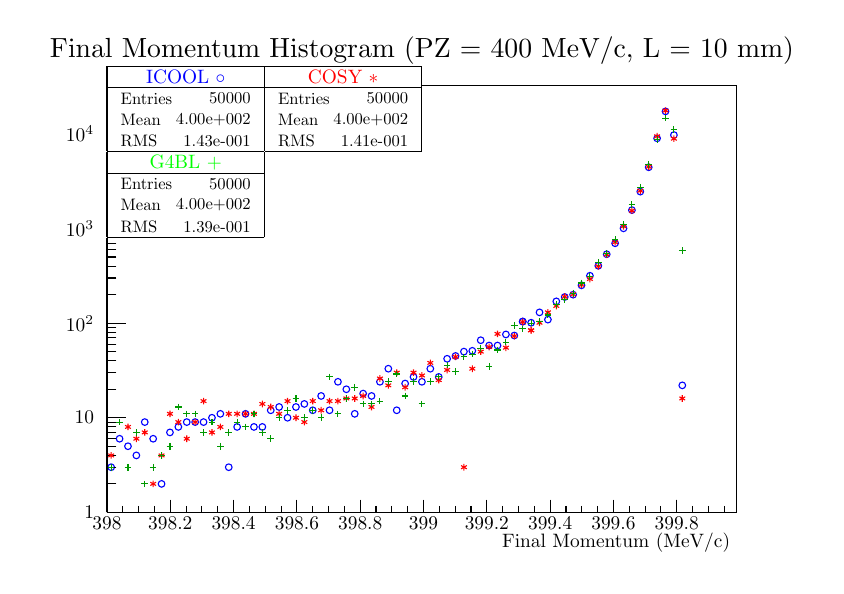
\begin{tikzpicture}
\definecolor{c}{rgb}{1,1,1};
\draw [color=c, fill=c] (0,0) rectangle (20,13.5632);
\draw [color=c, fill=c] (2,1.35632) rectangle (18,12.2069);
\definecolor{c}{rgb}{0,0,0};
\draw [c] (2,1.35632) -- (2,12.2069) -- (18,12.2069) -- (18,1.35632) -- (2,1.35632);
\definecolor{c}{rgb}{1,1,1};
\draw [color=c, fill=c] (2,1.35632) rectangle (18,12.2069);
\definecolor{c}{rgb}{0,0,0};
\draw [c] (2,1.35632) -- (2,12.2069) -- (18,12.2069) -- (18,1.35632) -- (2,1.35632);
\definecolor{c}{rgb}{0,0,1};
\foreach \P in
 {(2.10667,2.50282),(2.32,3.22618),(2.53333,3.03591),(2.74667,2.80304),(2.96,3.64932),(3.17333,3.22618),(3.38667,2.07968),(3.6,3.38705),(3.81333,3.5264),(4.02667,3.64932),(4.24,3.64932),(4.45333,3.64932),(4.66667,3.75927),(4.88,3.85874),(5.09333,2.50
282),(5.30667,3.5264),(5.52,3.85874),(5.73333,3.5264),(5.94667,3.5264),(6.16,3.94954),(6.37333,4.03307),(6.58667,3.75927),(6.8,4.03307),(7.01333,4.11041),(7.22667,3.94954),(7.44,4.31303),(7.65333,3.94954),(7.86667,4.6729),(8.08,4.48263),(8.29333,3.85
874),(8.50667,4.37268),(8.72,4.31303),(8.93333,4.6729),(9.14667,5.00524),(9.36,3.94954),(9.57333,4.62849),(9.78667,4.79582),(10,4.6729),(10.2133,5.00524),(10.4267,4.79582),(10.64,5.25691),(10.8533,5.32891),(11.0667,5.43886),(11.28,5.45953),(11.4933,5
.7286),(11.7067,5.59375),(11.92,5.59375),(12.1333,5.87583),(12.3467,5.84799),(12.56,6.20316)}{\draw[mark options={color=c,fill=c},mark size=2.402402pt,mark=o] plot coordinates {\P};}
\foreach \P in
 {(12.56,6.20316),(12.7733,6.17261),(12.9867,6.43603),(13.2,6.25216),(13.4133,6.71598),(13.6267,6.82655),(13.84,6.88559),(14.0533,7.12262),(14.2667,7.36625),(14.48,7.61933),(14.6933,7.91242),(14.9067,8.19146),(15.12,8.57038),(15.3333,9.03325),(15.546
7,9.50288),(15.76,10.1215),(15.9733,10.8567),(16.1867,11.54),(16.4,10.9398),(16.6133,4.5821)}{\draw[mark options={color=c,fill=c},mark size=2.402402pt,mark=o] plot coordinates {\P};}
\definecolor{c}{rgb}{1,1,1};
\draw [color=c, fill=c] (2,10.5115) rectangle (6,12.6816);
\definecolor{c}{rgb}{0,0,0};
\draw [c] (2,10.5115) -- (6,10.5115);
\draw [c] (6,10.5115) -- (6,12.6816);
\draw [c] (6,12.6816) -- (2,12.6816);
\draw [c] (2,12.6816) -- (2,10.5115);
\draw[color=blue](4,12.4103) node[scale=0.7, rotate=0]{ICOOL $\circ$};
\draw [c] (2,12.1391) -- (6,12.1391);
\draw [anchor= west] (2.2,11.8678) node[scale=0.6, rotate=0]{Entries };
\draw [anchor= east] (5.8,11.8678) node[scale=0.6, rotate=0]{ 50000};
\draw [anchor= west] (2.2,11.3253) node[scale=0.6, rotate=0]{Mean  };
\draw [anchor= east] (5.8,11.3253) node[scale=0.6, rotate=0]{ 4.00e+002};
\draw [anchor= west] (2.2,10.7828) node[scale=0.6, rotate=0]{RMS   };
\draw [anchor= east] (5.8,10.7828) node[scale=0.6, rotate=0]{ 1.43e-001};
\draw [c] (2,1.35632) -- (18,1.35632);
\draw [anchor= east] (18,0.596782) node[scale=0.7, rotate=0]{Final Momentum (MeV/c)};
\draw [c] (2,1.68184) -- (2,1.35632);
\draw [c] (2.40201,1.51908) -- (2.40201,1.35632);
\draw [c] (2.80402,1.51908) -- (2.80402,1.35632);
\draw [c] (3.20603,1.51908) -- (3.20603,1.35632);
\draw [c] (3.60804,1.68184) -- (3.60804,1.35632);
\draw [c] (4.01005,1.51908) -- (4.01005,1.35632);
\draw [c] (4.41206,1.51908) -- (4.41206,1.35632);
\draw [c] (4.81407,1.51908) -- (4.81407,1.35632);
\draw [c] (5.21608,1.68184) -- (5.21608,1.35632);
\draw [c] (5.61809,1.51908) -- (5.61809,1.35632);
\draw [c] (6.0201,1.51908) -- (6.0201,1.35632);
\draw [c] (6.42211,1.51908) -- (6.42211,1.35632);
\draw [c] (6.82412,1.68184) -- (6.82412,1.35632);
\draw [c] (7.22613,1.51908) -- (7.22613,1.35632);
\draw [c] (7.62814,1.51908) -- (7.62814,1.35632);
\draw [c] (8.03015,1.51908) -- (8.03015,1.35632);
\draw [c] (8.43216,1.68184) -- (8.43216,1.35632);
\draw [c] (8.83417,1.51908) -- (8.83417,1.35632);
\draw [c] (9.23618,1.51908) -- (9.23618,1.35632);
\draw [c] (9.63819,1.51908) -- (9.63819,1.35632);
\draw [c] (10.0402,1.68184) -- (10.0402,1.35632);
\draw [c] (10.4422,1.51908) -- (10.4422,1.35632);
\draw [c] (10.8442,1.51908) -- (10.8442,1.35632);
\draw [c] (11.2462,1.51908) -- (11.2462,1.35632);
\draw [c] (11.6482,1.68184) -- (11.6482,1.35632);
\draw [c] (12.0503,1.51908) -- (12.0503,1.35632);
\draw [c] (12.4523,1.51908) -- (12.4523,1.35632);
\draw [c] (12.8543,1.51908) -- (12.8543,1.35632);
\draw [c] (13.2563,1.68184) -- (13.2563,1.35632);
\draw [c] (13.6583,1.51908) -- (13.6583,1.35632);
\draw [c] (14.0603,1.51908) -- (14.0603,1.35632);
\draw [c] (14.4623,1.51908) -- (14.4623,1.35632);
\draw [c] (14.8643,1.68184) -- (14.8643,1.35632);
\draw [c] (15.2663,1.51908) -- (15.2663,1.35632);
\draw [c] (15.6683,1.51908) -- (15.6683,1.35632);
\draw [c] (16.0704,1.51908) -- (16.0704,1.35632);
\draw [c] (16.4724,1.68184) -- (16.4724,1.35632);
\draw [c] (16.4724,1.68184) -- (16.4724,1.35632);
\draw [c] (16.8744,1.51908) -- (16.8744,1.35632);
\draw [c] (17.2764,1.51908) -- (17.2764,1.35632);
\draw [c] (17.6784,1.51908) -- (17.6784,1.35632);
\draw [anchor=base] (2,0.908736) node[scale=0.7, rotate=0]{398};
\draw [anchor=base] (3.60804,0.908736) node[scale=0.7, rotate=0]{398.2};
\draw [anchor=base] (5.21608,0.908736) node[scale=0.7, rotate=0]{398.4};
\draw [anchor=base] (6.82412,0.908736) node[scale=0.7, rotate=0]{398.6};
\draw [anchor=base] (8.43216,0.908736) node[scale=0.7, rotate=0]{398.8};
\draw [anchor=base] (10.0402,0.908736) node[scale=0.7, rotate=0]{399};
\draw [anchor=base] (11.6482,0.908736) node[scale=0.7, rotate=0]{399.2};
\draw [anchor=base] (13.2563,0.908736) node[scale=0.7, rotate=0]{399.4};
\draw [anchor=base] (14.8643,0.908736) node[scale=0.7, rotate=0]{399.6};
\draw [anchor=base] (16.4724,0.908736) node[scale=0.7, rotate=0]{399.8};
\draw [c] (2,1.35632) -- (2,12.2069);
\draw [c] (2.48,1.35632) -- (2,1.35632);
\draw [anchor= east] (1.844,1.35632) node[scale=0.7, rotate=0]{1};
\draw [c] (2.24,2.07968) -- (2,2.07968);
\draw [c] (2.24,2.50282) -- (2,2.50282);
\draw [c] (2.24,2.80304) -- (2,2.80304);
\draw [c] (2.24,3.03591) -- (2,3.03591);
\draw [c] (2.24,3.22618) -- (2,3.22618);
\draw [c] (2.24,3.38705) -- (2,3.38705);
\draw [c] (2.24,3.52641) -- (2,3.52641);
\draw [c] (2.24,3.64932) -- (2,3.64932);
\draw [c] (2.48,3.75928) -- (2,3.75928);
\draw [anchor= east] (1.844,3.75928) node[scale=0.7, rotate=0]{10};
\draw [c] (2.24,4.48264) -- (2,4.48264);
\draw [c] (2.24,4.90577) -- (2,4.90577);
\draw [c] (2.24,5.206) -- (2,5.206);
\draw [c] (2.24,5.43887) -- (2,5.43887);
\draw [c] (2.24,5.62913) -- (2,5.62913);
\draw [c] (2.24,5.79) -- (2,5.79);
\draw [c] (2.24,5.92936) -- (2,5.92936);
\draw [c] (2.24,6.05227) -- (2,6.05227);
\draw [c] (2.48,6.16223) -- (2,6.16223);
\draw [anchor= east] (1.844,6.16223) node[scale=0.7, rotate=0]{$10^{2}$};
\draw [c] (2.24,6.88559) -- (2,6.88559);
\draw [c] (2.24,7.30872) -- (2,7.30872);
\draw [c] (2.24,7.60895) -- (2,7.60895);
\draw [c] (2.24,7.84182) -- (2,7.84182);
\draw [c] (2.24,8.03209) -- (2,8.03209);
\draw [c] (2.24,8.19296) -- (2,8.19296);
\draw [c] (2.24,8.33231) -- (2,8.33231);
\draw [c] (2.24,8.45522) -- (2,8.45522);
\draw [c] (2.48,8.56518) -- (2,8.56518);
\draw [anchor= east] (1.844,8.56518) node[scale=0.7, rotate=0]{$10^{3}$};
\draw [c] (2.24,9.28854) -- (2,9.28854);
\draw [c] (2.24,9.71168) -- (2,9.71168);
\draw [c] (2.24,10.0119) -- (2,10.0119);
\draw [c] (2.24,10.2448) -- (2,10.2448);
\draw [c] (2.24,10.435) -- (2,10.435);
\draw [c] (2.24,10.5959) -- (2,10.5959);
\draw [c] (2.24,10.7353) -- (2,10.7353);
\draw [c] (2.24,10.8582) -- (2,10.8582);
\draw [c] (2.48,10.9681) -- (2,10.9681);
\draw [anchor= east] (1.844,10.9681) node[scale=0.7, rotate=0]{$10^{4}$};
\draw [c] (2.24,11.6915) -- (2,11.6915);
\draw [c] (2.24,12.1146) -- (2,12.1146);
\definecolor{c}{rgb}{1,1,1};
\draw [color=c, fill=c] (2,10.5115) rectangle (6,12.6816);
\definecolor{c}{rgb}{0,0,0};
\draw [c] (2,10.5115) -- (6,10.5115);
\draw [c] (6,10.5115) -- (6,12.6816);
\draw [c] (6,12.6816) -- (2,12.6816);
\draw [c] (2,12.6816) -- (2,10.5115);
\draw[color=blue](4,12.4103) node[scale=0.7, rotate=0]{ICOOL $\circ$};
\draw [c] (2,12.1391) -- (6,12.1391);
\draw [anchor= west] (2.2,11.8678) node[scale=0.6, rotate=0]{Entries };
\draw [anchor= east] (5.8,11.8678) node[scale=0.6, rotate=0]{ 50000};
\draw [anchor= west] (2.2,11.3253) node[scale=0.6, rotate=0]{Mean  };
\draw [anchor= east] (5.8,11.3253) node[scale=0.6, rotate=0]{ 4.00e+002};
\draw [anchor= west] (2.2,10.7828) node[scale=0.6, rotate=0]{RMS   };
\draw [anchor= east] (5.8,10.7828) node[scale=0.6, rotate=0]{ 1.43e-001};
\draw (10,13.0816) node[scale=1, rotate=0]{Final Momentum Histogram (PZ = 400 MeV/c, L = 10 mm)};
\definecolor{c}{rgb}{1,0,0};
\foreach \P in
 {(2.10667,2.80304),(2.53333,3.5264),(2.74667,3.22618),(2.96,3.38705),(3.17333,2.07968),(3.38667,2.80304),(3.6,3.85874),(3.81333,3.64932),(4.02667,3.22618),(4.24,3.64932),(4.45333,4.18241),(4.66667,3.38705),(4.88,3.5264),(5.09333,3.85874),(5.30667,3.
85874),(5.52,3.85874),(5.73333,3.85874),(5.94667,4.11041),(6.16,4.03307),(6.37333,3.85874),(6.58667,4.18241),(6.8,3.75927),(7.01333,3.64932),(7.22667,4.18241),(7.44,3.94954),(7.65333,4.18241),(7.86667,4.18241),(8.08,4.24976),(8.29333,4.24976),(8.5066
7,4.31303),(8.72,4.03307),(8.93333,4.75643),(9.14667,4.5821),(9.36,4.90577),(9.57333,4.53355),(9.78667,4.90577),(10,4.83377),(10.2133,5.15246),(10.4267,4.7155),(10.64,4.97312),(10.8533,5.30546),(11.0667,2.50282),(11.28,5.00524),(11.4933,5.43886),(11.
7067,5.55713),(11.92,5.88947),(12.1333,5.53833),(12.3467,5.8338),(12.56,6.19307),(12.7733,5.98027)}{\draw[mark options={color=c,fill=c},mark size=2.402402pt,mark=asterisk] plot coordinates {\P};}
\foreach \P in
 {(12.7733,5.98027),(12.9867,6.17261),(13.2,6.43603),(13.4133,6.59919),(13.6267,6.83206),(13.84,6.89597),(14.0533,7.13502),(14.2667,7.28408),(14.48,7.60895),(14.6933,7.90459),(14.9067,8.21654),(15.12,8.62204),(15.3333,9.01916),(15.5467,9.52432),(15.7
6,10.1343),(15.9733,10.9086),(16.1867,11.5612),(16.4,10.848),(16.6133,4.24976)}{\draw[mark options={color=c,fill=c},mark size=2.402402pt,mark=asterisk] plot coordinates {\P};}
\definecolor{c}{rgb}{1,1,1};
\draw [color=c, fill=c] (6,10.5115) rectangle (10,12.6816);
\definecolor{c}{rgb}{0,0,0};
\draw [c] (6,10.5115) -- (10,10.5115);
\draw [c] (10,10.5115) -- (10,12.6816);
\draw [c] (10,12.6816) -- (6,12.6816);
\draw [c] (6,12.6816) -- (6,10.5115);
\draw [color=red](8,12.4103) node[scale=0.7, rotate=0]{COSY $*$};
\draw [c] (6,12.1391) -- (10,12.1391);
\draw [anchor= west] (6.2,11.8678) node[scale=0.6, rotate=0]{Entries };
\draw [anchor= east] (9.8,11.8678) node[scale=0.6, rotate=0]{ 50000};
\draw [anchor= west] (6.2,11.3253) node[scale=0.6, rotate=0]{Mean  };
\draw [anchor= east] (9.8,11.3253) node[scale=0.6, rotate=0]{ 4.00e+002};
\draw [anchor= west] (6.2,10.7828) node[scale=0.6, rotate=0]{RMS   };
\draw [anchor= east] (9.8,10.7828) node[scale=0.6, rotate=0]{ 1.41e-001};
\definecolor{c}{rgb}{1,1,1};
\draw [color=c, fill=c] (6,10.5115) rectangle (10,12.6816);
\definecolor{c}{rgb}{0,0,0};
\draw [c] (6,10.5115) -- (10,10.5115);
\draw [c] (10,10.5115) -- (10,12.6816);
\draw [c] (10,12.6816) -- (6,12.6816);
\draw [c] (6,12.6816) -- (6,10.5115);
\draw [color=red](8,12.4103) node[scale=0.7, rotate=0]{COSY $*$};
\draw [c] (6,12.1391) -- (10,12.1391);
\draw [anchor= west] (6.2,11.8678) node[scale=0.6, rotate=0]{Entries };
\draw [anchor= east] (9.8,11.8678) node[scale=0.6, rotate=0]{ 50000};
\draw [anchor= west] (6.2,11.3253) node[scale=0.6, rotate=0]{Mean  };
\draw [anchor= east] (9.8,11.3253) node[scale=0.6, rotate=0]{ 4.00e+002};
\draw [anchor= west] (6.2,10.7828) node[scale=0.6, rotate=0]{RMS   };
\draw [anchor= east] (9.8,10.7828) node[scale=0.6, rotate=0]{ 1.41e-001};
\definecolor{c}{rgb}{0,0.6,0};
\foreach \P in
 {(2.10667,2.50282),(2.32,3.64932),(2.53333,2.50282),(2.74667,3.38705),(2.96,2.07968),(3.17333,2.50282),(3.38667,2.80304),(3.6,3.03591),(3.81333,4.03307),(4.02667,3.85874),(4.24,3.85874),(4.45333,3.38705),(4.66667,3.64932),(4.88,3.03591),(5.09333,3.3
8705),(5.30667,3.64932),(5.52,3.5264),(5.73333,3.85874),(5.94667,3.38705),(6.16,3.22618),(6.37333,3.75927),(6.58667,3.94954),(6.8,4.24976),(7.01333,3.75927),(7.22667,3.94954),(7.44,3.75927),(7.65333,4.79582),(7.86667,3.85874),(8.08,4.24976),(8.29333,
4.53355),(8.50667,4.11041),(8.72,4.11041),(8.93333,4.18241),(9.14667,4.6729),(9.36,4.87039),(9.57333,4.31303),(9.78667,4.6729),(10,4.11041),(10.2133,4.6729),(10.4267,4.79582),(10.64,5.09604),(10.8533,4.93999),(11.0667,5.30546),(11.28,5.37429),(11.493
3,5.51918),(11.7067,5.06664),(11.92,5.47979),(12.1333,5.68005),(12.3467,6.1087),(12.56,6.01689)}{\draw[mark options={color=c,fill=c},mark size=2.402402pt,mark=+] plot coordinates {\P};}
\foreach \P in
 {(12.56,6.01689),(12.7733,6.16222),(12.9867,6.20316),(13.2,6.36974),(13.4133,6.63959),(13.6267,6.75218),(13.84,6.92149),(14.0533,7.18319),(14.2667,7.3463),(14.48,7.70841),(14.6933,7.92791),(14.9067,8.2897),(15.12,8.66654),(15.3333,9.16927),(15.5467,
9.61631),(15.76,10.1991),(15.9733,10.8192),(16.1867,11.3705),(16.4,11.0823),(16.6133,8.011)}{\draw[mark options={color=c,fill=c},mark size=2.402402pt,mark=+] plot coordinates {\P};}
\definecolor{c}{rgb}{1,1,1};
\draw [color=c, fill=c] (2,8.34138) rectangle (6,10.5115);
\definecolor{c}{rgb}{0,0,0};
\draw [c] (2,8.34138) -- (6,8.34138);
\draw [c] (6,8.34138) -- (6,10.5115);
\draw [c] (6,10.5115) -- (2,10.5115);
\draw [c] (2,10.5115) -- (2,8.34138);
\draw [color=green](4,10.2402) node[scale=0.7, rotate=0]{G4BL $+$};
\draw [c] (2,9.96897) -- (6,9.96897);
\draw [anchor= west] (2.2,9.6977) node[scale=0.6, rotate=0]{Entries };
\draw [anchor= east] (5.8,9.6977) node[scale=0.6, rotate=0]{ 50000};
\draw [anchor= west] (2.2,9.15517) node[scale=0.6, rotate=0]{Mean  };
\draw [anchor= east] (5.8,9.15517) node[scale=0.6, rotate=0]{ 4.00e+002};
\draw [anchor= west] (2.2,8.61264) node[scale=0.6, rotate=0]{RMS   };
\draw [anchor= east] (5.8,8.61264) node[scale=0.6, rotate=0]{ 1.39e-001};
\definecolor{c}{rgb}{1,1,1};
\draw [color=c, fill=c] (2,8.34138) rectangle (6,10.5115);
\definecolor{c}{rgb}{0,0,0};
\draw [c] (2,8.34138) -- (6,8.34138);
\draw [c] (6,8.34138) -- (6,10.5115);
\draw [c] (6,10.5115) -- (2,10.5115);
\draw [c] (2,10.5115) -- (2,8.34138);
\draw [color=green](4,10.2402) node[scale=0.7, rotate=0]{G4BL $+$};
\draw [c] (2,9.96897) -- (6,9.96897);
\draw [anchor= west] (2.2,9.6977) node[scale=0.6, rotate=0]{Entries };
\draw [anchor= east] (5.8,9.6977) node[scale=0.6, rotate=0]{ 50000};
\draw [anchor= west] (2.2,9.15517) node[scale=0.6, rotate=0]{Mean  };
\draw [anchor= east] (5.8,9.15517) node[scale=0.6, rotate=0]{ 4.00e+002};
\draw [anchor= west] (2.2,8.61264) node[scale=0.6, rotate=0]{RMS   };
\draw [anchor= east] (5.8,8.61264) node[scale=0.6, rotate=0]{ 1.39e-001};
\end{tikzpicture}
}\\
\frame{      \pgfdeclareplotmark{cross} {
\pgfpathmoveto{\pgfpoint{-0.3\pgfplotmarksize}{\pgfplotmarksize}}
\pgfpathlineto{\pgfpoint{+0.3\pgfplotmarksize}{\pgfplotmarksize}}
\pgfpathlineto{\pgfpoint{+0.3\pgfplotmarksize}{0.3\pgfplotmarksize}}
\pgfpathlineto{\pgfpoint{+1\pgfplotmarksize}{0.3\pgfplotmarksize}}
\pgfpathlineto{\pgfpoint{+1\pgfplotmarksize}{-0.3\pgfplotmarksize}}
\pgfpathlineto{\pgfpoint{+0.3\pgfplotmarksize}{-0.3\pgfplotmarksize}}
\pgfpathlineto{\pgfpoint{+0.3\pgfplotmarksize}{-1.\pgfplotmarksize}}
\pgfpathlineto{\pgfpoint{-0.3\pgfplotmarksize}{-1.\pgfplotmarksize}}
\pgfpathlineto{\pgfpoint{-0.3\pgfplotmarksize}{-0.3\pgfplotmarksize}}
\pgfpathlineto{\pgfpoint{-1.\pgfplotmarksize}{-0.3\pgfplotmarksize}}
\pgfpathlineto{\pgfpoint{-1.\pgfplotmarksize}{0.3\pgfplotmarksize}}
\pgfpathlineto{\pgfpoint{-0.3\pgfplotmarksize}{0.3\pgfplotmarksize}}
\pgfpathclose
\pgfusepathqstroke
}
\pgfdeclareplotmark{cross*} {
\pgfpathmoveto{\pgfpoint{-0.3\pgfplotmarksize}{\pgfplotmarksize}}
\pgfpathlineto{\pgfpoint{+0.3\pgfplotmarksize}{\pgfplotmarksize}}
\pgfpathlineto{\pgfpoint{+0.3\pgfplotmarksize}{0.3\pgfplotmarksize}}
\pgfpathlineto{\pgfpoint{+1\pgfplotmarksize}{0.3\pgfplotmarksize}}
\pgfpathlineto{\pgfpoint{+1\pgfplotmarksize}{-0.3\pgfplotmarksize}}
\pgfpathlineto{\pgfpoint{+0.3\pgfplotmarksize}{-0.3\pgfplotmarksize}}
\pgfpathlineto{\pgfpoint{+0.3\pgfplotmarksize}{-1.\pgfplotmarksize}}
\pgfpathlineto{\pgfpoint{-0.3\pgfplotmarksize}{-1.\pgfplotmarksize}}
\pgfpathlineto{\pgfpoint{-0.3\pgfplotmarksize}{-0.3\pgfplotmarksize}}
\pgfpathlineto{\pgfpoint{-1.\pgfplotmarksize}{-0.3\pgfplotmarksize}}
\pgfpathlineto{\pgfpoint{-1.\pgfplotmarksize}{0.3\pgfplotmarksize}}
\pgfpathlineto{\pgfpoint{-0.3\pgfplotmarksize}{0.3\pgfplotmarksize}}
\pgfpathclose
\pgfusepathqfillstroke
}
\pgfdeclareplotmark{newstar} {
\pgfpathmoveto{\pgfqpoint{0pt}{\pgfplotmarksize}}
\pgfpathlineto{\pgfqpointpolar{44}{0.5\pgfplotmarksize}}
\pgfpathlineto{\pgfqpointpolar{18}{\pgfplotmarksize}}
\pgfpathlineto{\pgfqpointpolar{-20}{0.5\pgfplotmarksize}}
\pgfpathlineto{\pgfqpointpolar{-54}{\pgfplotmarksize}}
\pgfpathlineto{\pgfqpointpolar{-90}{0.5\pgfplotmarksize}}
\pgfpathlineto{\pgfqpointpolar{234}{\pgfplotmarksize}}
\pgfpathlineto{\pgfqpointpolar{198}{0.5\pgfplotmarksize}}
\pgfpathlineto{\pgfqpointpolar{162}{\pgfplotmarksize}}
\pgfpathlineto{\pgfqpointpolar{134}{0.5\pgfplotmarksize}}
\pgfpathclose
\pgfusepathqstroke
}
\pgfdeclareplotmark{newstar*} {
\pgfpathmoveto{\pgfqpoint{0pt}{\pgfplotmarksize}}
\pgfpathlineto{\pgfqpointpolar{44}{0.5\pgfplotmarksize}}
\pgfpathlineto{\pgfqpointpolar{18}{\pgfplotmarksize}}
\pgfpathlineto{\pgfqpointpolar{-20}{0.5\pgfplotmarksize}}
\pgfpathlineto{\pgfqpointpolar{-54}{\pgfplotmarksize}}
\pgfpathlineto{\pgfqpointpolar{-90}{0.5\pgfplotmarksize}}
\pgfpathlineto{\pgfqpointpolar{234}{\pgfplotmarksize}}
\pgfpathlineto{\pgfqpointpolar{198}{0.5\pgfplotmarksize}}
\pgfpathlineto{\pgfqpointpolar{162}{\pgfplotmarksize}}
\pgfpathlineto{\pgfqpointpolar{134}{0.5\pgfplotmarksize}}
\pgfpathclose
\pgfusepathqfillstroke
}
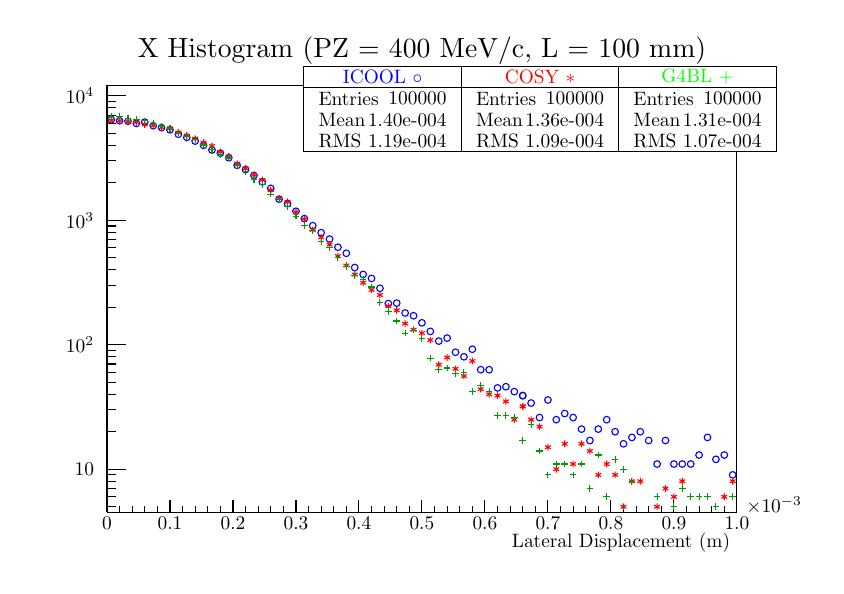
\begin{tikzpicture}
\definecolor{c}{rgb}{1,1,1};
\draw [color=c, fill=c] (0,0) rectangle (20,13.5632);
\draw [color=c, fill=c] (2,1.35632) rectangle (18,12.2069);
\definecolor{c}{rgb}{0,0,0};
\draw [c] (2,1.35632) -- (2,12.2069) -- (18,12.2069) -- (18,1.35632) -- (2,1.35632);
\definecolor{c}{rgb}{1,1,1};
\draw [color=c, fill=c] (2,1.35632) rectangle (18,12.2069);
\definecolor{c}{rgb}{0,0,0};
\draw [c] (2,1.35632) -- (2,12.2069) -- (18,12.2069) -- (18,1.35632) -- (2,1.35632);
\definecolor{c}{rgb}{0,0,1};
\foreach \P in
 {(2.10667,11.3295),(2.32,11.3043),(2.53333,11.2909),(2.74667,11.2356),(2.96,11.2681),(3.17333,11.1781),(3.38667,11.1283),(3.6,11.0736),(3.81333,10.9607),(4.02667,10.8813),(4.24,10.7869),(4.45333,10.6798),(4.66667,10.5598),(4.88,10.4805),(5.09333,10.
3626),(5.30667,10.17),(5.52,10.0625),(5.73333,9.91269),(5.94667,9.75061),(6.16,9.58443),(6.37333,9.31154),(6.58667,9.19832),(6.8,9.00356),(7.01333,8.81707),(7.22667,8.63811),(7.44,8.46019),(7.65333,8.29719),(7.86667,8.08976),(8.08,7.93679),(8.29333,7
.5743),(8.50667,7.39895),(8.72,7.29806),(8.93333,7.04695),(9.14667,6.65841),(9.36,6.67118),(9.57333,6.42087),(9.78667,6.35045),(10,6.17056),(10.2133,5.9528),(10.4267,5.70677),(10.64,5.78168),(10.8533,5.42269),(11.0667,5.30752),(11.28,5.49941),(11.493
3,4.97954),(11.7067,4.97954),(11.92,4.51759),(12.1333,4.54777),(12.3467,4.42287),(12.56,4.32113)}{\draw[mark options={color=c,fill=c},mark size=2.402402pt,mark=o] plot coordinates {\P};}
\foreach \P in
 {(12.56,4.32113),(12.7733,4.13276),(12.9867,3.76445),(13.2,4.21123),(13.4133,3.71061),(13.6267,3.8662),(13.84,3.76445),(14.0533,3.47123),(14.2667,3.18112),(14.48,3.47123),(14.6933,3.71061),(14.9067,3.40425),(15.12,3.09789),(15.3333,3.2596),(15.5467,
3.40425),(15.76,3.18112),(15.9733,2.58346),(16.1867,3.18112),(16.4,2.58346),(16.6133,2.58346),(16.8267,2.58346),(17.04,2.81282),(17.2533,3.2596),(17.4667,2.70292),(17.68,2.81282),(17.8933,2.30796)}{\draw[mark options={color=c,fill=c},mark
 size=2.402402pt,mark=o] plot coordinates {\P};}
\definecolor{c}{rgb}{1,1,1};
\draw [color=c, fill=c] (7,10.5115) rectangle (11,12.6816);
\definecolor{c}{rgb}{0,0,0};
\draw [c] (7,10.5115) -- (11,10.5115);
\draw [c] (11,10.5115) -- (11,12.6816);
\draw [c] (11,12.6816) -- (7,12.6816);
\draw [c] (7,12.6816) -- (7,10.5115);
\draw[color=blue](9,12.4103) node[scale=0.7, rotate=0]{ICOOL $\circ$};
\draw [c] (7,12.1391) -- (11,12.1391);
\draw [anchor= west] (7.2,11.8678) node[scale=0.7, rotate=0]{Entries };
\draw [anchor= east] (10.8,11.8678) node[scale=0.7, rotate=0]{ 100000};
\draw [anchor= west] (7.2,11.3253) node[scale=0.7, rotate=0]{Mean  };
\draw [anchor= east] (10.8,11.3253) node[scale=0.7, rotate=0]{ 1.40e-004};
\draw [anchor= west] (7.2,10.7828) node[scale=0.7, rotate=0]{RMS   };
\draw [anchor= east] (10.8,10.7828) node[scale=0.7, rotate=0]{ 1.19e-004};
\draw [c] (2,1.35632) -- (18,1.35632);
\draw [anchor= east] (18,0.596782) node[scale=0.7, rotate=0]{Lateral Displacement (m)};
\draw [c] (2,1.68184) -- (2,1.35632);
\draw [c] (2.32,1.51908) -- (2.32,1.35632);
\draw [c] (2.64,1.51908) -- (2.64,1.35632);
\draw [c] (2.96,1.51908) -- (2.96,1.35632);
\draw [c] (3.28,1.51908) -- (3.28,1.35632);
\draw [c] (3.6,1.68184) -- (3.6,1.35632);
\draw [c] (3.92,1.51908) -- (3.92,1.35632);
\draw [c] (4.24,1.51908) -- (4.24,1.35632);
\draw [c] (4.56,1.51908) -- (4.56,1.35632);
\draw [c] (4.88,1.51908) -- (4.88,1.35632);
\draw [c] (5.2,1.68184) -- (5.2,1.35632);
\draw [c] (5.52,1.51908) -- (5.52,1.35632);
\draw [c] (5.84,1.51908) -- (5.84,1.35632);
\draw [c] (6.16,1.51908) -- (6.16,1.35632);
\draw [c] (6.48,1.51908) -- (6.48,1.35632);
\draw [c] (6.8,1.68184) -- (6.8,1.35632);
\draw [c] (7.12,1.51908) -- (7.12,1.35632);
\draw [c] (7.44,1.51908) -- (7.44,1.35632);
\draw [c] (7.76,1.51908) -- (7.76,1.35632);
\draw [c] (8.08,1.51908) -- (8.08,1.35632);
\draw [c] (8.4,1.68184) -- (8.4,1.35632);
\draw [c] (8.72,1.51908) -- (8.72,1.35632);
\draw [c] (9.04,1.51908) -- (9.04,1.35632);
\draw [c] (9.36,1.51908) -- (9.36,1.35632);
\draw [c] (9.68,1.51908) -- (9.68,1.35632);
\draw [c] (10,1.68184) -- (10,1.35632);
\draw [c] (10.32,1.51908) -- (10.32,1.35632);
\draw [c] (10.64,1.51908) -- (10.64,1.35632);
\draw [c] (10.96,1.51908) -- (10.96,1.35632);
\draw [c] (11.28,1.51908) -- (11.28,1.35632);
\draw [c] (11.6,1.68184) -- (11.6,1.35632);
\draw [c] (11.92,1.51908) -- (11.92,1.35632);
\draw [c] (12.24,1.51908) -- (12.24,1.35632);
\draw [c] (12.56,1.51908) -- (12.56,1.35632);
\draw [c] (12.88,1.51908) -- (12.88,1.35632);
\draw [c] (13.2,1.68184) -- (13.2,1.35632);
\draw [c] (13.52,1.51908) -- (13.52,1.35632);
\draw [c] (13.84,1.51908) -- (13.84,1.35632);
\draw [c] (14.16,1.51908) -- (14.16,1.35632);
\draw [c] (14.48,1.51908) -- (14.48,1.35632);
\draw [c] (14.8,1.68184) -- (14.8,1.35632);
\draw [c] (15.12,1.51908) -- (15.12,1.35632);
\draw [c] (15.44,1.51908) -- (15.44,1.35632);
\draw [c] (15.76,1.51908) -- (15.76,1.35632);
\draw [c] (16.08,1.51908) -- (16.08,1.35632);
\draw [c] (16.4,1.68184) -- (16.4,1.35632);
\draw [c] (16.72,1.51908) -- (16.72,1.35632);
\draw [c] (17.04,1.51908) -- (17.04,1.35632);
\draw [c] (17.36,1.51908) -- (17.36,1.35632);
\draw [c] (17.68,1.51908) -- (17.68,1.35632);
\draw [c] (18,1.68184) -- (18,1.35632);
\draw [anchor=base] (2,0.908736) node[scale=0.7, rotate=0]{0};
\draw [anchor=base] (3.6,0.908736) node[scale=0.7, rotate=0]{0.1};
\draw [anchor=base] (5.2,0.908736) node[scale=0.7, rotate=0]{0.2};
\draw [anchor=base] (6.8,0.908736) node[scale=0.7, rotate=0]{0.3};
\draw [anchor=base] (8.4,0.908736) node[scale=0.7, rotate=0]{0.4};
\draw [anchor=base] (10,0.908736) node[scale=0.7, rotate=0]{0.5};
\draw [anchor=base] (11.6,0.908736) node[scale=0.7, rotate=0]{0.6};
\draw [anchor=base] (13.2,0.908736) node[scale=0.7, rotate=0]{0.7};
\draw [anchor=base] (14.8,0.908736) node[scale=0.7, rotate=0]{0.8};
\draw [anchor=base] (16.4,0.908736) node[scale=0.7, rotate=0]{0.9};
\draw [anchor=base] (18,0.908736) node[scale=0.7, rotate=0]{1.0};
\draw [anchor=base west] (18.07,1.35632) node[scale=0.7, rotate=0]{$\times10^{-3}$};
\draw [c] (2,1.35632) -- (2,12.2069);
\draw [c] (2.24,1.50097) -- (2,1.50097);
\draw [c] (2.24,1.75128) -- (2,1.75128);
\draw [c] (2.24,1.96292) -- (2,1.96292);
\draw [c] (2.24,2.14625) -- (2,2.14625);
\draw [c] (2.24,2.30796) -- (2,2.30796);
\draw [c] (2.48,2.45261) -- (2,2.45261);
\draw [anchor= east] (1.844,2.45261) node[scale=0.7, rotate=0]{10};
\draw [c] (2.24,3.40425) -- (2,3.40425);
\draw [c] (2.24,3.96092) -- (2,3.96092);
\draw [c] (2.24,4.35588) -- (2,4.35588);
\draw [c] (2.24,4.66224) -- (2,4.66224);
\draw [c] (2.24,4.91256) -- (2,4.91256);
\draw [c] (2.24,5.12419) -- (2,5.12419);
\draw [c] (2.24,5.30752) -- (2,5.30752);
\draw [c] (2.24,5.46923) -- (2,5.46923);
\draw [c] (2.48,5.61388) -- (2,5.61388);
\draw [anchor= east] (1.844,5.61388) node[scale=0.7, rotate=0]{$10^{2}$};
\draw [c] (2.24,6.56552) -- (2,6.56552);
\draw [c] (2.24,7.12219) -- (2,7.12219);
\draw [c] (2.24,7.51716) -- (2,7.51716);
\draw [c] (2.24,7.82352) -- (2,7.82352);
\draw [c] (2.24,8.07383) -- (2,8.07383);
\draw [c] (2.24,8.28547) -- (2,8.28547);
\draw [c] (2.24,8.46879) -- (2,8.46879);
\draw [c] (2.24,8.6305) -- (2,8.6305);
\draw [c] (2.48,8.77515) -- (2,8.77515);
\draw [anchor= east] (1.844,8.77515) node[scale=0.7, rotate=0]{$10^{3}$};
\draw [c] (2.24,9.72679) -- (2,9.72679);
\draw [c] (2.24,10.2835) -- (2,10.2835);
\draw [c] (2.24,10.6784) -- (2,10.6784);
\draw [c] (2.24,10.9848) -- (2,10.9848);
\draw [c] (2.24,11.2351) -- (2,11.2351);
\draw [c] (2.24,11.4467) -- (2,11.4467);
\draw [c] (2.24,11.6301) -- (2,11.6301);
\draw [c] (2.24,11.7918) -- (2,11.7918);
\draw [c] (2.48,11.9364) -- (2,11.9364);
\draw [anchor= east] (1.844,11.9364) node[scale=0.7, rotate=0]{$10^{4}$};
\definecolor{c}{rgb}{1,1,1};
\draw [color=c, fill=c] (7,10.5115) rectangle (11,12.6816);
\definecolor{c}{rgb}{0,0,0};
\draw [c] (7,10.5115) -- (11,10.5115);
\draw [c] (11,10.5115) -- (11,12.6816);
\draw [c] (11,12.6816) -- (7,12.6816);
\draw [c] (7,12.6816) -- (7,10.5115);
\draw[color=blue](9,12.4103) node[scale=0.7, rotate=0]{ICOOL $\circ$};
\draw [c] (7,12.1391) -- (11,12.1391);
\draw [anchor= west] (7.2,11.8678) node[scale=0.7, rotate=0]{Entries };
\draw [anchor= east] (10.8,11.8678) node[scale=0.7, rotate=0]{ 100000};
\draw [anchor= west] (7.2,11.3253) node[scale=0.7, rotate=0]{Mean  };
\draw [anchor= east] (10.8,11.3253) node[scale=0.7, rotate=0]{ 1.40e-004};
\draw [anchor= west] (7.2,10.7828) node[scale=0.7, rotate=0]{RMS   };
\draw [anchor= east] (10.8,10.7828) node[scale=0.7, rotate=0]{ 1.19e-004};
\draw (10,13.0816) node[scale=1, rotate=0]{X Histogram (PZ = 400 MeV/c, L = 100 mm)};
\definecolor{c}{rgb}{1,0,0};
\foreach \P in
 {(2.10667,11.314),(2.32,11.3036),(2.53333,11.2755),(2.74667,11.2661),(2.96,11.2097),(3.17333,11.1848),(3.38667,11.131),(3.6,11.1099),(3.81333,11.0044),(4.02667,10.9273),(4.24,10.849),(4.45333,10.7506),(4.66667,10.6619),(4.88,10.5115),(5.09333,10.394
6),(5.30667,10.2116),(5.52,10.0917),(5.73333,9.92819),(5.94667,9.7977),(6.16,9.53875),(6.37333,9.33091),(6.58667,9.24395),(6.8,8.98129),(7.01333,8.80503),(7.22667,8.53087),(7.44,8.34308),(7.65333,8.15814),(7.86667,7.86676),(8.08,7.62599),(8.29333,7.3
952),(8.50667,7.18918),(8.72,7.00772),(8.93333,6.87736),(9.14667,6.59271),(9.36,6.48785),(9.57333,6.15213),(9.78667,5.99505),(10,5.90921),(10.2133,5.7322),(10.4267,5.10444),(10.64,5.29025),(10.8533,5.00117),(11.0667,4.81784),(11.28,5.20049),(11.4933,
4.48674),(11.7067,4.35589),(11.92,4.32113),(12.1333,4.17256),(12.3467,3.71061),(12.56,4.04953)}{\draw[mark options={color=c,fill=c},mark size=2.402402pt,mark=asterisk] plot coordinates {\P};}
\foreach \P in
 {(12.56,4.04953),(12.7733,3.71061),(12.9867,3.5351),(13.2,3.00928),(13.4133,2.45261),(13.6267,3.09789),(13.84,2.58346),(14.0533,3.09789),(14.2667,2.91456),(14.48,2.30796),(14.6933,2.58346),(14.9067,2.30796),(15.12,1.50097),(15.3333,2.14625),(15.5467
,2.14625),(15.9733,1.50097),(16.1867,1.96292),(16.4,1.75129),(16.6133,2.14625),(17.68,1.75129),(17.8933,2.14625)}{\draw[mark options={color=c,fill=c},mark size=2.402402pt,mark=asterisk] plot coordinates {\P};}
\definecolor{c}{rgb}{1,1,1};
\draw [color=c, fill=c] (11,10.5115) rectangle (15,12.6816);
\definecolor{c}{rgb}{0,0,0};
\draw [c] (11,10.5115) -- (15,10.5115);
\draw [c] (15,10.5115) -- (15,12.6816);
\draw [c] (15,12.6816) -- (11,12.6816);
\draw [c] (11,12.6816) -- (11,10.5115);
\draw [color=red](13,12.4103) node[scale=0.7, rotate=0]{COSY $*$};
\draw [c] (11,12.1391) -- (15,12.1391);
\draw [anchor= west] (11.2,11.8678) node[scale=0.7, rotate=0]{Entries };
\draw [anchor= east] (14.8,11.8678) node[scale=0.7, rotate=0]{ 100000};
\draw [anchor= west] (11.2,11.3253) node[scale=0.7, rotate=0]{Mean  };
\draw [anchor= east] (14.8,11.3253) node[scale=0.7, rotate=0]{ 1.36e-004};
\draw [anchor= west] (11.2,10.7828) node[scale=0.7, rotate=0]{RMS   };
\draw [anchor= east] (14.8,10.7828) node[scale=0.7, rotate=0]{ 1.09e-004};
\definecolor{c}{rgb}{1,1,1};
\draw [color=c, fill=c] (11,10.5115) rectangle (15,12.6816);
\definecolor{c}{rgb}{0,0,0};
\draw [c] (11,10.5115) -- (15,10.5115);
\draw [c] (15,10.5115) -- (15,12.6816);
\draw [c] (15,12.6816) -- (11,12.6816);
\draw [c] (11,12.6816) -- (11,10.5115);
\draw [color=red](13,12.4103) node[scale=0.7, rotate=0]{COSY $*$};
\draw [c] (11,12.1391) -- (15,12.1391);
\draw [anchor= west] (11.2,11.8678) node[scale=0.7, rotate=0]{Entries };
\draw [anchor= east] (14.8,11.8678) node[scale=0.7, rotate=0]{ 100000};
\draw [anchor= west] (11.2,11.3253) node[scale=0.7, rotate=0]{Mean  };
\draw [anchor= east] (14.8,11.3253) node[scale=0.7, rotate=0]{ 1.36e-004};
\draw [anchor= west] (11.2,10.7828) node[scale=0.7, rotate=0]{RMS   };
\draw [anchor= east] (14.8,10.7828) node[scale=0.7, rotate=0]{ 1.09e-004};
\definecolor{c}{rgb}{0,0.6,0};
\foreach \P in
 {(2.10667,11.4047),(2.32,11.4124),(2.53333,11.363),(2.74667,11.3361),(2.96,11.2993),(3.17333,11.2328),(3.38667,11.1692),(3.6,11.1008),(3.81333,10.9963),(4.02667,10.9068),(4.24,10.8263),(4.45333,10.687),(4.66667,10.5699),(4.88,10.4513),(5.09333,10.35
65),(5.30667,10.161),(5.52,10.0054),(5.73333,9.8055),(5.94667,9.67717),(6.16,9.43834),(6.37333,9.29378),(6.58667,9.12476),(6.8,8.87954),(7.01333,8.65019),(7.22667,8.51603),(7.44,8.2396),(7.65333,8.07383),(7.86667,7.83446),(8.08,7.60684),(8.29333,7.36
869),(8.50667,7.28186),(8.72,7.08037),(8.93333,6.68384),(9.14667,6.45104),(9.36,6.21557),(9.57333,5.90921),(9.78667,5.98461),(10,5.76947),(10.2133,5.27276),(10.4267,4.97954),(10.64,5.02245),(10.8533,4.88948),(11.0667,4.91256),(11.28,4.42287),(11.4933
,4.5773),(11.7067,4.42287),(11.92,3.81627),(12.1333,3.81627),(12.3467,3.76445),(12.56,3.18112)}{\draw[mark options={color=c,fill=c},mark size=2.402402pt,mark=+] plot coordinates {\P};}
\foreach \P in
 {(12.56,3.18112),(12.7733,3.59613),(12.9867,2.91456),(13.2,2.30796),(13.4133,2.58346),(13.6267,2.58346),(13.84,2.30796),(14.0533,2.58346),(14.2667,1.96292),(14.48,2.81282),(14.6933,1.75129),(14.9067,2.70292),(15.12,2.45261),(15.3333,2.14625),(15.973
3,1.75129),(16.4,1.50097),(16.6133,1.96292),(16.8267,1.75129),(17.04,1.75129),(17.2533,1.75129),(17.4667,1.50097),(17.8933,1.75129)}{\draw[mark options={color=c,fill=c},mark size=2.402402pt,mark=+] plot coordinates {\P};}
\definecolor{c}{rgb}{1,1,1};
\draw [color=c, fill=c] (15,10.5115) rectangle (19,12.6816);
\definecolor{c}{rgb}{0,0,0};
\draw [c] (15,10.5115) -- (19,10.5115);
\draw [c] (19,10.5115) -- (19,12.6816);
\draw [c] (19,12.6816) -- (15,12.6816);
\draw [c] (15,12.6816) -- (15,10.5115);
\draw [color=green](17,12.4103) node[scale=0.7, rotate=0]{G4BL $+$};
\draw [c] (15,12.1391) -- (19,12.1391);
\draw [anchor= west] (15.2,11.8678) node[scale=0.7, rotate=0]{Entries };
\draw [anchor= east] (18.8,11.8678) node[scale=0.7, rotate=0]{ 100000};
\draw [anchor= west] (15.2,11.3253) node[scale=0.7, rotate=0]{Mean  };
\draw [anchor= east] (18.8,11.3253) node[scale=0.7, rotate=0]{ 1.31e-004};
\draw [anchor= west] (15.2,10.7828) node[scale=0.7, rotate=0]{RMS   };
\draw [anchor= east] (18.8,10.7828) node[scale=0.7, rotate=0]{ 1.07e-004};
\definecolor{c}{rgb}{1,1,1};
\draw [color=c, fill=c] (15,10.5115) rectangle (19,12.6816);
\definecolor{c}{rgb}{0,0,0};
\draw [c] (15,10.5115) -- (19,10.5115);
\draw [c] (19,10.5115) -- (19,12.6816);
\draw [c] (19,12.6816) -- (15,12.6816);
\draw [c] (15,12.6816) -- (15,10.5115);
\draw [color=green](17,12.4103) node[scale=0.7, rotate=0]{G4BL $+$};
\draw [c] (15,12.1391) -- (19,12.1391);
\draw [anchor= west] (15.2,11.8678) node[scale=0.7, rotate=0]{Entries };
\draw [anchor= east] (18.8,11.8678) node[scale=0.7, rotate=0]{ 100000};
\draw [anchor= west] (15.2,11.3253) node[scale=0.7, rotate=0]{Mean  };
\draw [anchor= east] (18.8,11.3253) node[scale=0.7, rotate=0]{ 1.31e-004};
\draw [anchor= west] (15.2,10.7828) node[scale=0.7, rotate=0]{RMS   };
\draw [anchor= east] (18.8,10.7828) node[scale=0.7, rotate=0]{ 1.07e-004};
\end{tikzpicture}
}\\
\frame{    \pgfdeclareplotmark{cross} {
\pgfpathmoveto{\pgfpoint{-0.3\pgfplotmarksize}{\pgfplotmarksize}}
\pgfpathlineto{\pgfpoint{+0.3\pgfplotmarksize}{\pgfplotmarksize}}
\pgfpathlineto{\pgfpoint{+0.3\pgfplotmarksize}{0.3\pgfplotmarksize}}
\pgfpathlineto{\pgfpoint{+1\pgfplotmarksize}{0.3\pgfplotmarksize}}
\pgfpathlineto{\pgfpoint{+1\pgfplotmarksize}{-0.3\pgfplotmarksize}}
\pgfpathlineto{\pgfpoint{+0.3\pgfplotmarksize}{-0.3\pgfplotmarksize}}
\pgfpathlineto{\pgfpoint{+0.3\pgfplotmarksize}{-1.\pgfplotmarksize}}
\pgfpathlineto{\pgfpoint{-0.3\pgfplotmarksize}{-1.\pgfplotmarksize}}
\pgfpathlineto{\pgfpoint{-0.3\pgfplotmarksize}{-0.3\pgfplotmarksize}}
\pgfpathlineto{\pgfpoint{-1.\pgfplotmarksize}{-0.3\pgfplotmarksize}}
\pgfpathlineto{\pgfpoint{-1.\pgfplotmarksize}{0.3\pgfplotmarksize}}
\pgfpathlineto{\pgfpoint{-0.3\pgfplotmarksize}{0.3\pgfplotmarksize}}
\pgfpathclose
\pgfusepathqstroke
}
\pgfdeclareplotmark{cross*} {
\pgfpathmoveto{\pgfpoint{-0.3\pgfplotmarksize}{\pgfplotmarksize}}
\pgfpathlineto{\pgfpoint{+0.3\pgfplotmarksize}{\pgfplotmarksize}}
\pgfpathlineto{\pgfpoint{+0.3\pgfplotmarksize}{0.3\pgfplotmarksize}}
\pgfpathlineto{\pgfpoint{+1\pgfplotmarksize}{0.3\pgfplotmarksize}}
\pgfpathlineto{\pgfpoint{+1\pgfplotmarksize}{-0.3\pgfplotmarksize}}
\pgfpathlineto{\pgfpoint{+0.3\pgfplotmarksize}{-0.3\pgfplotmarksize}}
\pgfpathlineto{\pgfpoint{+0.3\pgfplotmarksize}{-1.\pgfplotmarksize}}
\pgfpathlineto{\pgfpoint{-0.3\pgfplotmarksize}{-1.\pgfplotmarksize}}
\pgfpathlineto{\pgfpoint{-0.3\pgfplotmarksize}{-0.3\pgfplotmarksize}}
\pgfpathlineto{\pgfpoint{-1.\pgfplotmarksize}{-0.3\pgfplotmarksize}}
\pgfpathlineto{\pgfpoint{-1.\pgfplotmarksize}{0.3\pgfplotmarksize}}
\pgfpathlineto{\pgfpoint{-0.3\pgfplotmarksize}{0.3\pgfplotmarksize}}
\pgfpathclose
\pgfusepathqfillstroke
}
\pgfdeclareplotmark{newstar} {
\pgfpathmoveto{\pgfqpoint{0pt}{\pgfplotmarksize}}
\pgfpathlineto{\pgfqpointpolar{44}{0.5\pgfplotmarksize}}
\pgfpathlineto{\pgfqpointpolar{18}{\pgfplotmarksize}}
\pgfpathlineto{\pgfqpointpolar{-20}{0.5\pgfplotmarksize}}
\pgfpathlineto{\pgfqpointpolar{-54}{\pgfplotmarksize}}
\pgfpathlineto{\pgfqpointpolar{-90}{0.5\pgfplotmarksize}}
\pgfpathlineto{\pgfqpointpolar{234}{\pgfplotmarksize}}
\pgfpathlineto{\pgfqpointpolar{198}{0.5\pgfplotmarksize}}
\pgfpathlineto{\pgfqpointpolar{162}{\pgfplotmarksize}}
\pgfpathlineto{\pgfqpointpolar{134}{0.5\pgfplotmarksize}}
\pgfpathclose
\pgfusepathqstroke
}
\pgfdeclareplotmark{newstar*} {
\pgfpathmoveto{\pgfqpoint{0pt}{\pgfplotmarksize}}
\pgfpathlineto{\pgfqpointpolar{44}{0.5\pgfplotmarksize}}
\pgfpathlineto{\pgfqpointpolar{18}{\pgfplotmarksize}}
\pgfpathlineto{\pgfqpointpolar{-20}{0.5\pgfplotmarksize}}
\pgfpathlineto{\pgfqpointpolar{-54}{\pgfplotmarksize}}
\pgfpathlineto{\pgfqpointpolar{-90}{0.5\pgfplotmarksize}}
\pgfpathlineto{\pgfqpointpolar{234}{\pgfplotmarksize}}
\pgfpathlineto{\pgfqpointpolar{198}{0.5\pgfplotmarksize}}
\pgfpathlineto{\pgfqpointpolar{162}{\pgfplotmarksize}}
\pgfpathlineto{\pgfqpointpolar{134}{0.5\pgfplotmarksize}}
\pgfpathclose
\pgfusepathqfillstroke
}
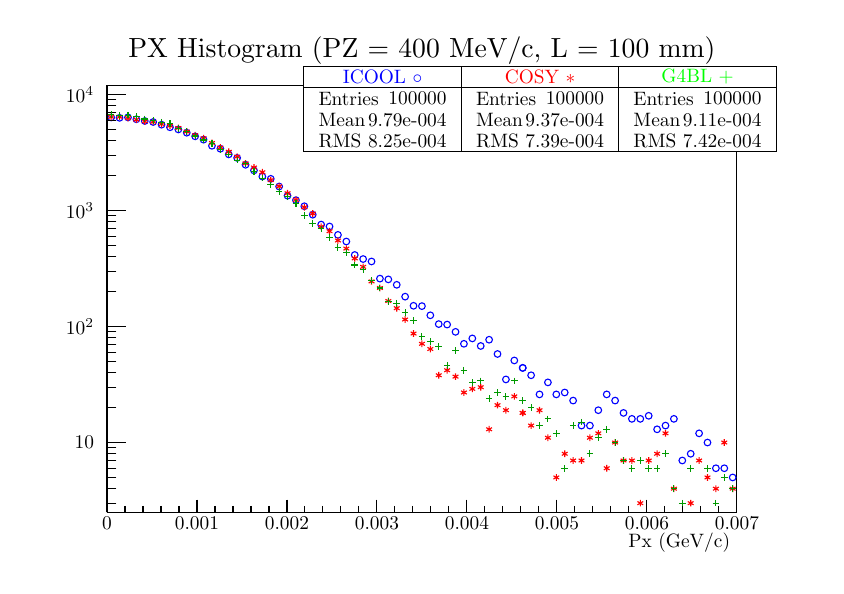
\begin{tikzpicture}
\definecolor{c}{rgb}{1,1,1};
\draw [color=c, fill=c] (0,0) rectangle (20,13.5632);
\draw [color=c, fill=c] (2,1.35632) rectangle (18,12.2069);
\definecolor{c}{rgb}{0,0,0};
\draw [c] (2,1.35632) -- (2,12.2069) -- (18,12.2069) -- (18,1.35632) -- (2,1.35632);
\definecolor{c}{rgb}{1,1,1};
\draw [color=c, fill=c] (2,1.35632) rectangle (18,12.2069);
\definecolor{c}{rgb}{0,0,0};
\draw [c] (2,1.35632) -- (2,12.2069) -- (18,12.2069) -- (18,1.35632) -- (2,1.35632);
\definecolor{c}{rgb}{0,0,1};
\foreach \P in
 {(2.10667,11.387),(2.32,11.3771),(2.53333,11.3892),(2.74667,11.3409),(2.96,11.2965),(3.17333,11.2714),(3.38667,11.2034),(3.6,11.1376),(3.81333,11.0821),(4.02667,10.9991),(4.24,10.9073),(4.45333,10.8231),(4.66667,10.6671),(4.88,10.5914),(5.09333,10.4
49),(5.30667,10.3596),(5.52,10.185),(5.73333,10.0422),(5.94667,9.88613),(6.16,9.82819),(6.37333,9.63278),(6.58667,9.40015),(6.8,9.28571),(7.01333,9.13215),(7.22667,8.9166),(7.44,8.66571),(7.65333,8.61749),(7.86667,8.40408),(8.08,8.2359),(8.29333,7.89
359),(8.50667,7.79067),(8.72,7.72891),(8.93333,7.29349),(9.14667,7.27358),(9.36,7.13599),(9.57333,6.83504),(9.78667,6.60319),(10,6.59469),(10.2133,6.36142),(10.4267,6.13835),(10.64,6.12611),(10.8533,5.94113),(11.0667,5.63774),(11.28,5.77434),(11.4933
,5.58251),(11.7067,5.74154),(11.92,5.379),(12.1333,4.73277),(12.3467,5.21444),(12.56,5.02555)}{\draw[mark options={color=c,fill=c},mark size=2.402402pt,mark=o] plot coordinates {\P};}
\foreach \P in
 {(12.56,5.02555),(12.7733,4.83799),(12.9867,4.35246),(13.2,4.65749),(13.4133,4.35246),(13.6267,4.40075),(13.84,4.1956),(14.0533,3.56046),(14.2667,3.56046),(14.48,3.95117),(14.6933,4.35246),(14.9067,4.1956),(15.12,3.88199),(15.3333,3.7313),(15.5467,3
.7313),(15.76,3.80886),(15.9733,3.46564),(16.1867,3.56046),(16.4,3.7313),(16.6133,2.67363),(16.8267,2.84447),(17.04,3.36323),(17.2533,3.12997),(17.4667,2.47641),(17.68,2.47641),(17.8933,2.24314)}{\draw[mark options={color=c,fill=c},mark
 size=2.402402pt,mark=o] plot coordinates {\P};}
\definecolor{c}{rgb}{1,1,1};
\draw [color=c, fill=c] (7,10.5115) rectangle (11,12.6816);
\definecolor{c}{rgb}{0,0,0};
\draw [c] (7,10.5115) -- (11,10.5115);
\draw [c] (11,10.5115) -- (11,12.6816);
\draw [c] (11,12.6816) -- (7,12.6816);
\draw [c] (7,12.6816) -- (7,10.5115);
\draw[color=blue](9,12.4103) node[scale=0.7, rotate=0]{ICOOL $\circ$};
\draw [c] (7,12.1391) -- (11,12.1391);
\draw [anchor= west] (7.2,11.8678) node[scale=0.6, rotate=0]{Entries };
\draw [anchor= east] (10.8,11.8678) node[scale=0.6, rotate=0]{ 100000};
\draw [anchor= west] (7.2,11.3253) node[scale=0.6, rotate=0]{Mean  };
\draw [anchor= east] (10.8,11.3253) node[scale=0.6, rotate=0]{ 9.79e-004};
\draw [anchor= west] (7.2,10.7828) node[scale=0.6, rotate=0]{RMS   };
\draw [anchor= east] (10.8,10.7828) node[scale=0.6, rotate=0]{ 8.25e-004};
\draw [c] (2,1.35632) -- (18,1.35632);
\draw [anchor= east] (18,0.596782) node[scale=0.7, rotate=0]{Px (GeV/c)};
\draw [c] (2,1.68184) -- (2,1.35632);
\draw [c] (2.45714,1.51908) -- (2.45714,1.35632);
\draw [c] (2.91429,1.51908) -- (2.91429,1.35632);
\draw [c] (3.37143,1.51908) -- (3.37143,1.35632);
\draw [c] (3.82857,1.51908) -- (3.82857,1.35632);
\draw [c] (4.28571,1.68184) -- (4.28571,1.35632);
\draw [c] (4.74286,1.51908) -- (4.74286,1.35632);
\draw [c] (5.2,1.51908) -- (5.2,1.35632);
\draw [c] (5.65714,1.51908) -- (5.65714,1.35632);
\draw [c] (6.11429,1.51908) -- (6.11429,1.35632);
\draw [c] (6.57143,1.68184) -- (6.57143,1.35632);
\draw [c] (7.02857,1.51908) -- (7.02857,1.35632);
\draw [c] (7.48571,1.51908) -- (7.48571,1.35632);
\draw [c] (7.94286,1.51908) -- (7.94286,1.35632);
\draw [c] (8.4,1.51908) -- (8.4,1.35632);
\draw [c] (8.85714,1.68184) -- (8.85714,1.35632);
\draw [c] (9.31429,1.51908) -- (9.31429,1.35632);
\draw [c] (9.77143,1.51908) -- (9.77143,1.35632);
\draw [c] (10.2286,1.51908) -- (10.2286,1.35632);
\draw [c] (10.6857,1.51908) -- (10.6857,1.35632);
\draw [c] (11.1429,1.68184) -- (11.1429,1.35632);
\draw [c] (11.6,1.51908) -- (11.6,1.35632);
\draw [c] (12.0571,1.51908) -- (12.0571,1.35632);
\draw [c] (12.5143,1.51908) -- (12.5143,1.35632);
\draw [c] (12.9714,1.51908) -- (12.9714,1.35632);
\draw [c] (13.4286,1.68184) -- (13.4286,1.35632);
\draw [c] (13.8857,1.51908) -- (13.8857,1.35632);
\draw [c] (14.3429,1.51908) -- (14.3429,1.35632);
\draw [c] (14.8,1.51908) -- (14.8,1.35632);
\draw [c] (15.2571,1.51908) -- (15.2571,1.35632);
\draw [c] (15.7143,1.68184) -- (15.7143,1.35632);
\draw [c] (16.1714,1.51908) -- (16.1714,1.35632);
\draw [c] (16.6286,1.51908) -- (16.6286,1.35632);
\draw [c] (17.0857,1.51908) -- (17.0857,1.35632);
\draw [c] (17.5429,1.51908) -- (17.5429,1.35632);
\draw [c] (18,1.68184) -- (18,1.35632);
\draw [c] (18,1.68184) -- (18,1.35632);
\draw [anchor=base] (2,0.908736) node[scale=0.7, rotate=0]{0};
\draw [anchor=base] (4.28571,0.908736) node[scale=0.7, rotate=0]{0.001};
\draw [anchor=base] (6.57143,0.908736) node[scale=0.7, rotate=0]{0.002};
\draw [anchor=base] (8.85714,0.908736) node[scale=0.7, rotate=0]{0.003};
\draw [anchor=base] (11.1429,0.908736) node[scale=0.7, rotate=0]{0.004};
\draw [anchor=base] (13.4286,0.908736) node[scale=0.7, rotate=0]{0.005};
\draw [anchor=base] (15.7143,0.908736) node[scale=0.7, rotate=0]{0.006};
\draw [anchor=base] (18,0.908736) node[scale=0.7, rotate=0]{0.007};
\draw [c] (2,1.35632) -- (2,12.2069);
\draw [c] (2.24,1.58958) -- (2,1.58958);
\draw [c] (2.24,1.95765) -- (2,1.95765);
\draw [c] (2.24,2.24314) -- (2,2.24314);
\draw [c] (2.24,2.47641) -- (2,2.47641);
\draw [c] (2.24,2.67363) -- (2,2.67363);
\draw [c] (2.24,2.84447) -- (2,2.84447);
\draw [c] (2.24,2.99517) -- (2,2.99517);
\draw [c] (2.48,3.12997) -- (2,3.12997);
\draw [anchor= east] (1.844,3.12997) node[scale=0.7, rotate=0]{10};
\draw [c] (2.24,4.01679) -- (2,4.01679);
\draw [c] (2.24,4.53555) -- (2,4.53555);
\draw [c] (2.24,4.90361) -- (2,4.90361);
\draw [c] (2.24,5.1891) -- (2,5.1891);
\draw [c] (2.24,5.42237) -- (2,5.42237);
\draw [c] (2.24,5.61959) -- (2,5.61959);
\draw [c] (2.24,5.79043) -- (2,5.79043);
\draw [c] (2.24,5.94113) -- (2,5.94113);
\draw [c] (2.48,6.07593) -- (2,6.07593);
\draw [anchor= east] (1.844,6.07593) node[scale=0.7, rotate=0]{$10^{2}$};
\draw [c] (2.24,6.96275) -- (2,6.96275);
\draw [c] (2.24,7.48151) -- (2,7.48151);
\draw [c] (2.24,7.84957) -- (2,7.84957);
\draw [c] (2.24,8.13507) -- (2,8.13507);
\draw [c] (2.24,8.36833) -- (2,8.36833);
\draw [c] (2.24,8.56556) -- (2,8.56556);
\draw [c] (2.24,8.7364) -- (2,8.7364);
\draw [c] (2.24,8.88709) -- (2,8.88709);
\draw [c] (2.48,9.02189) -- (2,9.02189);
\draw [anchor= east] (1.844,9.02189) node[scale=0.7, rotate=0]{$10^{3}$};
\draw [c] (2.24,9.90871) -- (2,9.90871);
\draw [c] (2.24,10.4275) -- (2,10.4275);
\draw [c] (2.24,10.7955) -- (2,10.7955);
\draw [c] (2.24,11.081) -- (2,11.081);
\draw [c] (2.24,11.3143) -- (2,11.3143);
\draw [c] (2.24,11.5115) -- (2,11.5115);
\draw [c] (2.24,11.6824) -- (2,11.6824);
\draw [c] (2.24,11.8331) -- (2,11.8331);
\draw [c] (2.48,11.9679) -- (2,11.9679);
\draw [anchor= east] (1.844,11.9679) node[scale=0.7, rotate=0]{$10^{4}$};
\definecolor{c}{rgb}{1,1,1};
\draw [color=c, fill=c] (7,10.5115) rectangle (11,12.6816);
\definecolor{c}{rgb}{0,0,0};
\draw [c] (7,10.5115) -- (11,10.5115);
\draw [c] (11,10.5115) -- (11,12.6816);
\draw [c] (11,12.6816) -- (7,12.6816);
\draw [c] (7,12.6816) -- (7,10.5115);
\draw[color=blue](9,12.4103) node[scale=0.7, rotate=0]{ICOOL $\circ$};
\draw [c] (7,12.1391) -- (11,12.1391);
\draw [anchor= west] (7.2,11.8678) node[scale=0.7, rotate=0]{Entries };
\draw [anchor= east] (10.8,11.8678) node[scale=0.7, rotate=0]{ 100000};
\draw [anchor= west] (7.2,11.3253) node[scale=0.7, rotate=0]{Mean  };
\draw [anchor= east] (10.8,11.3253) node[scale=0.7, rotate=0]{ 9.79e-004};
\draw [anchor= west] (7.2,10.7828) node[scale=0.7, rotate=0]{RMS   };
\draw [anchor= east] (10.8,10.7828) node[scale=0.7, rotate=0]{ 8.25e-004};
\draw (10,13.0816) node[scale=1, rotate=0]{PX Histogram (PZ = 400 MeV/c, L = 100 mm)};
\definecolor{c}{rgb}{1,0,0};
\foreach \P in
 {(2.10667,11.4009),(2.32,11.4017),(2.53333,11.3714),(2.74667,11.3312),(2.96,11.2889),(3.17333,11.2755),(3.38667,11.2187),(3.6,11.1769),(3.81333,11.1208),(4.02667,11.0285),(4.24,10.9368),(4.45333,10.8601),(4.66667,10.7393),(4.88,10.6236),(5.09333,10.
5168),(5.30667,10.3911),(5.52,10.221),(5.73333,10.115),(5.94667,9.99528),(6.16,9.79576),(6.37333,9.63753),(6.58667,9.46239),(6.8,9.2909),(7.01333,9.10726),(7.22667,8.94545),(7.44,8.61222),(7.65333,8.49801),(7.86667,8.26165),(8.08,8.0559),(8.29333,7.8
073),(8.50667,7.59177),(8.72,7.2224),(8.93333,7.05528),(9.14667,6.72436),(9.36,6.54246),(9.57333,6.25474),(9.78667,5.89776),(10,5.63774),(10.2133,5.50494),(10.4267,4.83799),(10.64,4.96604),(10.8533,4.80387),(11.0667,4.40075),(11.28,4.49217),(11.4933,
4.53555),(11.7067,3.46564),(11.92,4.07921),(12.1333,3.95117),(12.3467,4.30228),(12.56,3.88199)}{\draw[mark options={color=c,fill=c},mark size=2.402402pt,mark=asterisk] plot coordinates {\P};}
\foreach \P in
 {(12.56,3.88199),(12.7733,3.56046),(12.9867,3.95117),(13.2,3.25191),(13.4133,2.24314),(13.6267,2.84447),(13.84,2.67363),(14.0533,2.67363),(14.2667,3.25191),(14.48,3.36323),(14.6933,2.47641),(14.9067,3.12997),(15.12,2.67363),(15.3333,2.67363),(15.546
7,1.58959),(15.76,2.67363),(15.9733,2.84447),(16.1867,3.36323),(16.4,1.95765),(16.8267,1.58959),(17.04,2.67363),(17.2533,2.24314),(17.4667,1.95765),(17.68,3.12997),(17.8933,1.95765)}{\draw[mark options={color=c,fill=c},mark
 size=2.402402pt,mark=asterisk] plot coordinates {\P};}
\definecolor{c}{rgb}{1,1,1};
\draw [color=c, fill=c] (11,10.5115) rectangle (15,12.6816);
\definecolor{c}{rgb}{0,0,0};
\draw [c] (11,10.5115) -- (15,10.5115);
\draw [c] (15,10.5115) -- (15,12.6816);
\draw [c] (15,12.6816) -- (11,12.6816);
\draw [c] (11,12.6816) -- (11,10.5115);
\draw [color=red](13,12.4103) node[scale=0.7, rotate=0]{COSY $*$};
\draw [c] (11,12.1391) -- (15,12.1391);
\draw [anchor= west] (11.2,11.8678) node[scale=0.7, rotate=0]{Entries };
\draw [anchor= east] (14.8,11.8678) node[scale=0.7, rotate=0]{ 100000};
\draw [anchor= west] (11.2,11.3253) node[scale=0.7, rotate=0]{Mean  };
\draw [anchor= east] (14.8,11.3253) node[scale=0.7, rotate=0]{ 9.37e-004};
\draw [anchor= west] (11.2,10.7828) node[scale=0.7, rotate=0]{RMS   };
\draw [anchor= east] (14.8,10.7828) node[scale=0.7, rotate=0]{ 7.39e-004};
\definecolor{c}{rgb}{1,1,1};
\draw [color=c, fill=c] (11,10.5115) rectangle (15,12.6816);
\definecolor{c}{rgb}{0,0,0};
\draw [c] (11,10.5115) -- (15,10.5115);
\draw [c] (15,10.5115) -- (15,12.6816);
\draw [c] (15,12.6816) -- (11,12.6816);
\draw [c] (11,12.6816) -- (11,10.5115);
\draw [color=red](13,12.4103) node[scale=0.7, rotate=0]{COSY $*$};
\draw [c] (11,12.1391) -- (15,12.1391);
\draw [anchor= west] (11.2,11.8678) node[scale=0.7, rotate=0]{Entries };
\draw [anchor= east] (14.8,11.8678) node[scale=0.7, rotate=0]{ 100000};
\draw [anchor= west] (11.2,11.3253) node[scale=0.7, rotate=0]{Mean  };
\draw [anchor= east] (14.8,11.3253) node[scale=0.7, rotate=0]{ 9.37e-004};
\draw [anchor= west] (11.2,10.7828) node[scale=0.7, rotate=0]{RMS   };
\draw [anchor= east] (14.8,10.7828) node[scale=0.7, rotate=0]{ 7.39e-004};
\definecolor{c}{rgb}{0,0.6,0};
\foreach \P in
 {(2.10667,11.4644),(2.32,11.4428),(2.53333,11.4465),(2.74667,11.4094),(2.96,11.3484),(3.17333,11.3102),(3.38667,11.2687),(3.6,11.2258),(3.81333,11.1124),(4.02667,11.0344),(4.24,10.9152),(4.45333,10.8146),(4.66667,10.7181),(4.88,10.5751),(5.09333,10.
4557),(5.30667,10.304),(5.52,10.209),(5.73333,10.009),(5.94667,9.84712),(6.16,9.67417),(6.37333,9.50957),(6.58667,9.38579),(6.8,9.20626),(7.01333,8.89418),(7.22667,8.6875),(7.44,8.55639),(7.65333,8.33594),(7.86667,8.09081),(8.08,7.951),(8.29333,7.637
88),(8.50667,7.51933),(8.72,7.23797),(8.93333,7.05528),(9.14667,6.70885),(9.36,6.66924),(9.57333,6.43114),(9.78667,6.2323),(10,5.82203),(10.2133,5.69069),(10.4267,5.56355),(10.64,5.08243),(10.8533,5.46432),(11.0667,4.96604),(11.28,4.65749),(11.4933,4
.69568),(11.7067,4.25006),(11.92,4.40075),(12.1333,4.30228),(12.3467,4.69568),(12.56,4.1956)}{\draw[mark options={color=c,fill=c},mark size=2.402402pt,mark=+] plot coordinates {\P};}
\foreach \P in
 {(12.56,4.1956),(12.7733,4.01679),(12.9867,3.56046),(13.2,3.7313),(13.4133,3.36323),(13.6267,2.47641),(13.84,3.56046),(14.0533,3.64873),(14.2667,2.84447),(14.48,3.25191),(14.6933,3.46564),(14.9067,3.12997),(15.12,2.67363),(15.3333,2.47641),(15.5467,
2.67363),(15.76,2.47641),(15.9733,2.47641),(16.1867,2.84447),(16.4,1.95765),(16.6133,1.58959),(16.8267,2.47641),(17.2533,2.47641),(17.4667,1.58959),(17.68,2.24314),(17.8933,1.95765)}{\draw[mark options={color=c,fill=c},mark size=2.402402pt,mark=+]
 plot coordinates {\P};}
\definecolor{c}{rgb}{1,1,1};
\draw [color=c, fill=c] (15,10.5115) rectangle (19,12.6816);
\definecolor{c}{rgb}{0,0,0};
\draw [c] (15,10.5115) -- (19,10.5115);
\draw [c] (19,10.5115) -- (19,12.6816);
\draw [c] (19,12.6816) -- (15,12.6816);
\draw [c] (15,12.6816) -- (15,10.5115);
\draw [color=green](17,12.4103) node[scale=0.7, rotate=0]{G4BL $+$};
\draw [c] (15,12.1391) -- (19,12.1391);
\draw [anchor= west] (15.2,11.8678) node[scale=0.7, rotate=0]{Entries };
\draw [anchor= east] (18.8,11.8678) node[scale=0.7, rotate=0]{ 100000};
\draw [anchor= west] (15.2,11.3253) node[scale=0.7, rotate=0]{Mean  };
\draw [anchor= east] (18.8,11.3253) node[scale=0.7, rotate=0]{ 9.11e-004};
\draw [anchor= west] (15.2,10.7828) node[scale=0.7, rotate=0]{RMS   };
\draw [anchor= east] (18.8,10.7828) node[scale=0.7, rotate=0]{ 7.42e-004};
\definecolor{c}{rgb}{1,1,1};
\draw [color=c, fill=c] (15,10.5115) rectangle (19,12.6816);
\definecolor{c}{rgb}{0,0,0};
\draw [c] (15,10.5115) -- (19,10.5115);
\draw [c] (19,10.5115) -- (19,12.6816);
\draw [c] (19,12.6816) -- (15,12.6816);
\draw [c] (15,12.6816) -- (15,10.5115);
\draw [color=green](17,12.4103) node[scale=0.7, rotate=0]{G4BL $+$};
\draw [c] (15,12.1391) -- (19,12.1391);
\draw [anchor= west] (15.2,11.8678) node[scale=0.7, rotate=0]{Entries };
\draw [anchor= east] (18.8,11.8678) node[scale=0.7, rotate=0]{ 100000};
\draw [anchor= west] (15.2,11.3253) node[scale=0.7, rotate=0]{Mean  };
\draw [anchor= east] (18.8,11.3253) node[scale=0.7, rotate=0]{ 9.11e-004};
\draw [anchor= west] (15.2,10.7828) node[scale=0.7, rotate=0]{RMS   };
\draw [anchor= east] (18.8,10.7828) node[scale=0.7, rotate=0]{ 7.42e-004};
\end{tikzpicture}
}\\
\frame{\pgfdeclareplotmark{cross} {
\pgfpathmoveto{\pgfpoint{-0.3\pgfplotmarksize}{\pgfplotmarksize}}
\pgfpathlineto{\pgfpoint{+0.3\pgfplotmarksize}{\pgfplotmarksize}}
\pgfpathlineto{\pgfpoint{+0.3\pgfplotmarksize}{0.3\pgfplotmarksize}}
\pgfpathlineto{\pgfpoint{+1\pgfplotmarksize}{0.3\pgfplotmarksize}}
\pgfpathlineto{\pgfpoint{+1\pgfplotmarksize}{-0.3\pgfplotmarksize}}
\pgfpathlineto{\pgfpoint{+0.3\pgfplotmarksize}{-0.3\pgfplotmarksize}}
\pgfpathlineto{\pgfpoint{+0.3\pgfplotmarksize}{-1.\pgfplotmarksize}}
\pgfpathlineto{\pgfpoint{-0.3\pgfplotmarksize}{-1.\pgfplotmarksize}}
\pgfpathlineto{\pgfpoint{-0.3\pgfplotmarksize}{-0.3\pgfplotmarksize}}
\pgfpathlineto{\pgfpoint{-1.\pgfplotmarksize}{-0.3\pgfplotmarksize}}
\pgfpathlineto{\pgfpoint{-1.\pgfplotmarksize}{0.3\pgfplotmarksize}}
\pgfpathlineto{\pgfpoint{-0.3\pgfplotmarksize}{0.3\pgfplotmarksize}}
\pgfpathclose
\pgfusepathqstroke
}
\pgfdeclareplotmark{cross*} {
\pgfpathmoveto{\pgfpoint{-0.3\pgfplotmarksize}{\pgfplotmarksize}}
\pgfpathlineto{\pgfpoint{+0.3\pgfplotmarksize}{\pgfplotmarksize}}
\pgfpathlineto{\pgfpoint{+0.3\pgfplotmarksize}{0.3\pgfplotmarksize}}
\pgfpathlineto{\pgfpoint{+1\pgfplotmarksize}{0.3\pgfplotmarksize}}
\pgfpathlineto{\pgfpoint{+1\pgfplotmarksize}{-0.3\pgfplotmarksize}}
\pgfpathlineto{\pgfpoint{+0.3\pgfplotmarksize}{-0.3\pgfplotmarksize}}
\pgfpathlineto{\pgfpoint{+0.3\pgfplotmarksize}{-1.\pgfplotmarksize}}
\pgfpathlineto{\pgfpoint{-0.3\pgfplotmarksize}{-1.\pgfplotmarksize}}
\pgfpathlineto{\pgfpoint{-0.3\pgfplotmarksize}{-0.3\pgfplotmarksize}}
\pgfpathlineto{\pgfpoint{-1.\pgfplotmarksize}{-0.3\pgfplotmarksize}}
\pgfpathlineto{\pgfpoint{-1.\pgfplotmarksize}{0.3\pgfplotmarksize}}
\pgfpathlineto{\pgfpoint{-0.3\pgfplotmarksize}{0.3\pgfplotmarksize}}
\pgfpathclose
\pgfusepathqfillstroke
}
\pgfdeclareplotmark{newstar} {
\pgfpathmoveto{\pgfqpoint{0pt}{\pgfplotmarksize}}
\pgfpathlineto{\pgfqpointpolar{44}{0.5\pgfplotmarksize}}
\pgfpathlineto{\pgfqpointpolar{18}{\pgfplotmarksize}}
\pgfpathlineto{\pgfqpointpolar{-20}{0.5\pgfplotmarksize}}
\pgfpathlineto{\pgfqpointpolar{-54}{\pgfplotmarksize}}
\pgfpathlineto{\pgfqpointpolar{-90}{0.5\pgfplotmarksize}}
\pgfpathlineto{\pgfqpointpolar{234}{\pgfplotmarksize}}
\pgfpathlineto{\pgfqpointpolar{198}{0.5\pgfplotmarksize}}
\pgfpathlineto{\pgfqpointpolar{162}{\pgfplotmarksize}}
\pgfpathlineto{\pgfqpointpolar{134}{0.5\pgfplotmarksize}}
\pgfpathclose
\pgfusepathqstroke
}
\pgfdeclareplotmark{newstar*} {
\pgfpathmoveto{\pgfqpoint{0pt}{\pgfplotmarksize}}
\pgfpathlineto{\pgfqpointpolar{44}{0.5\pgfplotmarksize}}
\pgfpathlineto{\pgfqpointpolar{18}{\pgfplotmarksize}}
\pgfpathlineto{\pgfqpointpolar{-20}{0.5\pgfplotmarksize}}
\pgfpathlineto{\pgfqpointpolar{-54}{\pgfplotmarksize}}
\pgfpathlineto{\pgfqpointpolar{-90}{0.5\pgfplotmarksize}}
\pgfpathlineto{\pgfqpointpolar{234}{\pgfplotmarksize}}
\pgfpathlineto{\pgfqpointpolar{198}{0.5\pgfplotmarksize}}
\pgfpathlineto{\pgfqpointpolar{162}{\pgfplotmarksize}}
\pgfpathlineto{\pgfqpointpolar{134}{0.5\pgfplotmarksize}}
\pgfpathclose
\pgfusepathqfillstroke
}
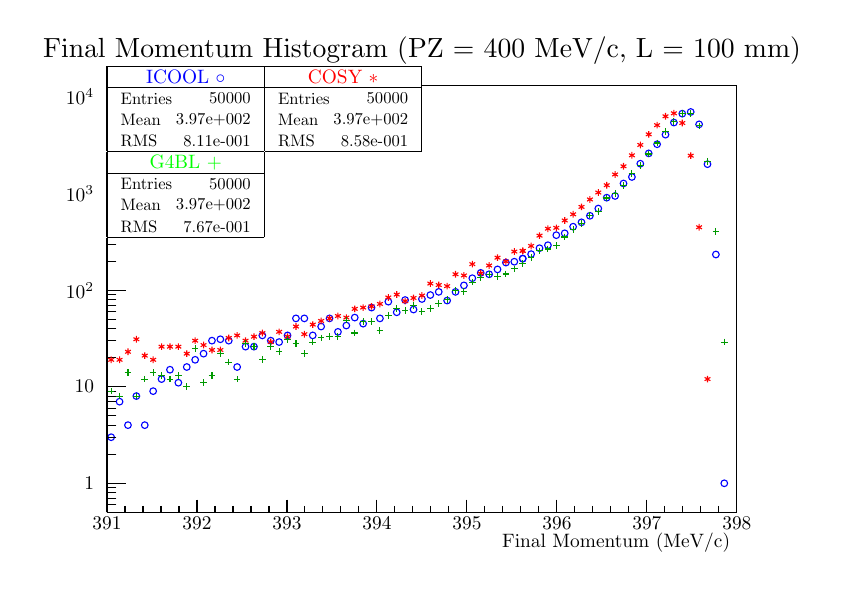
\begin{tikzpicture}
\definecolor{c}{rgb}{1,1,1};
\draw [color=c, fill=c] (0,0) rectangle (20,13.5632);
\draw [color=c, fill=c] (2,1.35632) rectangle (18,12.2069);
\definecolor{c}{rgb}{0,0,0};
\draw [c] (2,1.35632) -- (2,12.2069) -- (18,12.2069) -- (18,1.35632) -- (2,1.35632);
\definecolor{c}{rgb}{1,1,1};
\draw [color=c, fill=c] (2,1.35632) rectangle (18,12.2069);
\definecolor{c}{rgb}{0,0,0};
\draw [c] (2,1.35632) -- (2,12.2069) -- (18,12.2069) -- (18,1.35632) -- (2,1.35632);
\definecolor{c}{rgb}{0,0,1};
\foreach \P in
 {(2.10667,3.26498),(2.32,4.16755),(2.53333,3.57143),(2.74667,4.30979),(2.96,3.57143),(3.17333,4.43526),(3.38667,4.74171),(3.6,4.97941),(3.81333,4.64902),(4.02667,5.04816),(4.24,5.23123),(4.45333,5.38739),(4.66667,5.71778),(4.88,5.75271),(5.09333,5.7
1778),(5.30667,5.04816),(5.52,5.56535),(5.73333,5.56535),(5.94667,5.85111),(6.16,5.71778),(6.37333,5.68167),(6.58667,5.85111),(6.8,6.28303),(7.01333,6.28303),(7.22667,5.85111),(7.44,6.07621),(7.65333,6.28303),(7.86667,5.94118),(8.08,6.10127),(8.29333
,6.30371),(8.50667,6.1497),(8.72,6.55768),(8.93333,6.28303),(9.14667,6.70796),(9.36,6.43825),(9.57333,6.7492),(9.78667,6.50812),(10,6.77583),(10.2133,6.87617),(10.4267,6.95682),(10.64,6.73563),(10.8533,6.95682),(11.0667,7.12102),(11.28,7.30409),(11.4
933,7.4393),(11.7067,7.40343),(11.92,7.52727),(12.1333,7.70072),(12.3467,7.72257),(12.56,7.80074)}{\draw[mark options={color=c,fill=c},mark size=2.402402pt,mark=o] plot coordinates {\P};}
\foreach \P in
 {(12.56,7.80074),(12.7733,7.91498),(12.9867,8.06622),(13.2,8.1418),(13.4133,8.39687),(13.6267,8.44459),(13.84,8.61193),(14.0533,8.72323),(14.2667,8.88925),(14.48,9.07316),(14.6933,9.34913),(14.9067,9.39285),(15.12,9.7094),(15.3333,9.87504),(15.5467,
10.2115),(15.76,10.4742),(15.9733,10.7064),(16.1867,10.9502),(16.4,11.2568),(16.6133,11.483),(16.8267,11.5261),(17.04,11.2114),(17.2533,10.2),(17.4667,7.90592),(17.68,2.09469)}{\draw[mark options={color=c,fill=c},mark size=2.402402pt,mark=o] plot
 coordinates {\P};}
\definecolor{c}{rgb}{1,1,1};
\draw [color=c, fill=c] (2,10.5115) rectangle (6,12.6816);
\definecolor{c}{rgb}{0,0,0};
\draw [c] (2,10.5115) -- (6,10.5115);
\draw [c] (6,10.5115) -- (6,12.6816);
\draw [c] (6,12.6816) -- (2,12.6816);
\draw [c] (2,12.6816) -- (2,10.5115);
\draw[color=blue](4,12.4103) node[scale=0.7, rotate=0]{ICOOL $\circ$};
\draw [c] (2,12.1391) -- (6,12.1391);
\draw [anchor= west] (2.2,11.8678) node[scale=0.6, rotate=0]{Entries };
\draw [anchor= east] (5.8,11.8678) node[scale=0.6, rotate=0]{ 50000};
\draw [anchor= west] (2.2,11.3253) node[scale=0.6, rotate=0]{Mean  };
\draw [anchor= east] (5.8,11.3253) node[scale=0.6, rotate=0]{ 3.97e+002};
\draw [anchor= west] (2.2,10.7828) node[scale=0.6, rotate=0]{RMS   };
\draw [anchor= east] (5.8,10.7828) node[scale=0.6, rotate=0]{ 8.11e-001};
\draw [c] (2,1.35632) -- (18,1.35632);
\draw [anchor= east] (18,0.596782) node[scale=0.7, rotate=0]{Final Momentum (MeV/c)};
\draw [c] (2,1.68184) -- (2,1.35632);
\draw [c] (2.45714,1.51908) -- (2.45714,1.35632);
\draw [c] (2.91429,1.51908) -- (2.91429,1.35632);
\draw [c] (3.37143,1.51908) -- (3.37143,1.35632);
\draw [c] (3.82857,1.51908) -- (3.82857,1.35632);
\draw [c] (4.28571,1.68184) -- (4.28571,1.35632);
\draw [c] (4.74286,1.51908) -- (4.74286,1.35632);
\draw [c] (5.2,1.51908) -- (5.2,1.35632);
\draw [c] (5.65714,1.51908) -- (5.65714,1.35632);
\draw [c] (6.11429,1.51908) -- (6.11429,1.35632);
\draw [c] (6.57143,1.68184) -- (6.57143,1.35632);
\draw [c] (7.02857,1.51908) -- (7.02857,1.35632);
\draw [c] (7.48571,1.51908) -- (7.48571,1.35632);
\draw [c] (7.94286,1.51908) -- (7.94286,1.35632);
\draw [c] (8.4,1.51908) -- (8.4,1.35632);
\draw [c] (8.85714,1.68184) -- (8.85714,1.35632);
\draw [c] (9.31429,1.51908) -- (9.31429,1.35632);
\draw [c] (9.77143,1.51908) -- (9.77143,1.35632);
\draw [c] (10.2286,1.51908) -- (10.2286,1.35632);
\draw [c] (10.6857,1.51908) -- (10.6857,1.35632);
\draw [c] (11.1429,1.68184) -- (11.1429,1.35632);
\draw [c] (11.6,1.51908) -- (11.6,1.35632);
\draw [c] (12.0571,1.51908) -- (12.0571,1.35632);
\draw [c] (12.5143,1.51908) -- (12.5143,1.35632);
\draw [c] (12.9714,1.51908) -- (12.9714,1.35632);
\draw [c] (13.4286,1.68184) -- (13.4286,1.35632);
\draw [c] (13.8857,1.51908) -- (13.8857,1.35632);
\draw [c] (14.3429,1.51908) -- (14.3429,1.35632);
\draw [c] (14.8,1.51908) -- (14.8,1.35632);
\draw [c] (15.2571,1.51908) -- (15.2571,1.35632);
\draw [c] (15.7143,1.68184) -- (15.7143,1.35632);
\draw [c] (16.1714,1.51908) -- (16.1714,1.35632);
\draw [c] (16.6286,1.51908) -- (16.6286,1.35632);
\draw [c] (17.0857,1.51908) -- (17.0857,1.35632);
\draw [c] (17.5429,1.51908) -- (17.5429,1.35632);
\draw [c] (18,1.68184) -- (18,1.35632);
\draw [anchor=base] (2,0.908736) node[scale=0.7, rotate=0]{391};
\draw [anchor=base] (4.28571,0.908736) node[scale=0.7, rotate=0]{392};
\draw [anchor=base] (6.57143,0.908736) node[scale=0.7, rotate=0]{393};
\draw [anchor=base] (8.85714,0.908736) node[scale=0.7, rotate=0]{394};
\draw [anchor=base] (11.1429,0.908736) node[scale=0.7, rotate=0]{395};
\draw [anchor=base] (13.4286,0.908736) node[scale=0.7, rotate=0]{396};
\draw [anchor=base] (15.7143,0.908736) node[scale=0.7, rotate=0]{397};
\draw [anchor=base] (18,0.908736) node[scale=0.7, rotate=0]{398};
\draw [c] (2,1.35632) -- (2,12.2069);
\draw [c] (2.24,1.35632) -- (2,1.35632);
\draw [c] (2.24,1.55054) -- (2,1.55054);
\draw [c] (2.24,1.71475) -- (2,1.71475);
\draw [c] (2.24,1.85699) -- (2,1.85699);
\draw [c] (2.24,1.98246) -- (2,1.98246);
\draw [c] (2.48,2.09469) -- (2,2.09469);
\draw [anchor= east] (1.844,2.09469) node[scale=0.7, rotate=0]{1};
\draw [c] (2.24,2.83306) -- (2,2.83306);
\draw [c] (2.24,3.26498) -- (2,3.26498);
\draw [c] (2.24,3.57143) -- (2,3.57143);
\draw [c] (2.24,3.80913) -- (2,3.80913);
\draw [c] (2.24,4.00335) -- (2,4.00335);
\draw [c] (2.24,4.16755) -- (2,4.16755);
\draw [c] (2.24,4.3098) -- (2,4.3098);
\draw [c] (2.24,4.43526) -- (2,4.43526);
\draw [c] (2.48,4.5475) -- (2,4.5475);
\draw [anchor= east] (1.844,4.5475) node[scale=0.7, rotate=0]{10};
\draw [c] (2.24,5.28587) -- (2,5.28587);
\draw [c] (2.24,5.71778) -- (2,5.71778);
\draw [c] (2.24,6.02423) -- (2,6.02423);
\draw [c] (2.24,6.26194) -- (2,6.26194);
\draw [c] (2.24,6.45615) -- (2,6.45615);
\draw [c] (2.24,6.62036) -- (2,6.62036);
\draw [c] (2.24,6.7626) -- (2,6.7626);
\draw [c] (2.24,6.88807) -- (2,6.88807);
\draw [c] (2.48,7.0003) -- (2,7.0003);
\draw [anchor= east] (1.844,7.0003) node[scale=0.7, rotate=0]{$10^{2}$};
\draw [c] (2.24,7.73867) -- (2,7.73867);
\draw [c] (2.24,8.17059) -- (2,8.17059);
\draw [c] (2.24,8.47704) -- (2,8.47704);
\draw [c] (2.24,8.71474) -- (2,8.71474);
\draw [c] (2.24,8.90896) -- (2,8.90896);
\draw [c] (2.24,9.07316) -- (2,9.07316);
\draw [c] (2.24,9.21541) -- (2,9.21541);
\draw [c] (2.24,9.34087) -- (2,9.34087);
\draw [c] (2.48,9.45311) -- (2,9.45311);
\draw [anchor= east] (1.844,9.45311) node[scale=0.7, rotate=0]{$10^{3}$};
\draw [c] (2.24,10.1915) -- (2,10.1915);
\draw [c] (2.24,10.6234) -- (2,10.6234);
\draw [c] (2.24,10.9298) -- (2,10.9298);
\draw [c] (2.24,11.1675) -- (2,11.1675);
\draw [c] (2.24,11.3618) -- (2,11.3618);
\draw [c] (2.24,11.526) -- (2,11.526);
\draw [c] (2.24,11.6682) -- (2,11.6682);
\draw [c] (2.24,11.7937) -- (2,11.7937);
\draw [c] (2.48,11.9059) -- (2,11.9059);
\draw [anchor= east] (1.844,11.9059) node[scale=0.7, rotate=0]{$10^{4}$};
\definecolor{c}{rgb}{1,1,1};
\draw [color=c, fill=c] (2,10.5115) rectangle (6,12.6816);
\definecolor{c}{rgb}{0,0,0};
\draw [c] (2,10.5115) -- (6,10.5115);
\draw [c] (6,10.5115) -- (6,12.6816);
\draw [c] (6,12.6816) -- (2,12.6816);
\draw [c] (2,12.6816) -- (2,10.5115);
\draw[color=blue](4,12.4103) node[scale=0.7, rotate=0]{ICOOL $\circ$};
\draw [c] (2,12.1391) -- (6,12.1391);
\draw [anchor= west] (2.2,11.8678) node[scale=0.6, rotate=0]{Entries };
\draw [anchor= east] (5.8,11.8678) node[scale=0.6, rotate=0]{ 50000};
\draw [anchor= west] (2.2,11.3253) node[scale=0.6, rotate=0]{Mean  };
\draw [anchor= east] (5.8,11.3253) node[scale=0.6, rotate=0]{ 3.97e+002};
\draw [anchor= west] (2.2,10.7828) node[scale=0.6, rotate=0]{RMS   };
\draw [anchor= east] (5.8,10.7828) node[scale=0.6, rotate=0]{ 8.11e-001};
\draw (10,13.0816) node[scale=1, rotate=0]{Final Momentum Histogram (PZ = 400 MeV/c, L = 100 mm)};
\definecolor{c}{rgb}{1,0,0};
\foreach \P in
 {(2.10667,5.23123),(2.32,5.23123),(2.53333,5.43474),(2.74667,5.75271),(2.96,5.33784),(3.17333,5.23123),(3.38667,5.56535),(3.6,5.56535),(3.81333,5.56535),(4.02667,5.38739),(4.24,5.71778),(4.45333,5.60555),(4.66667,5.48008),(4.88,5.48008),(5.09333,5.7
8653),(5.30667,5.85111),(5.52,5.71778),(5.73333,5.81931),(5.94667,5.912),(6.16,5.68167),(6.37333,5.94118),(6.58667,5.81931),(6.8,6.07621),(7.01333,5.88199),(7.22667,6.12576),(7.44,6.21845),(7.65333,6.28303),(7.86667,6.34392),(8.08,6.30371),(8.29333,6
.5249),(8.50667,6.55768),(8.72,6.58948),(8.93333,6.65037),(9.14667,6.81457),(9.36,6.88807),(9.57333,6.72189),(9.78667,6.80182),(10,6.86413),(10.2133,7.16755),(10.4267,7.13049),(10.64,7.10183),(10.8533,7.40343),(11.0667,7.37384),(11.28,7.66137),(11.49
33,7.4251),(11.7067,7.62644),(11.92,7.82557),(12.1333,7.72796),(12.3467,7.98062),(12.56,7.99747)}{\draw[mark options={color=c,fill=c},mark size=2.402402pt,mark=asterisk] plot coordinates {\P};}
\foreach \P in
 {(12.56,7.99747),(12.7733,8.1234),(12.9867,8.38532),(13.2,8.56148),(13.4133,8.5834),(13.6267,8.77076),(13.84,8.92656),(14.0533,9.11494),(14.2667,9.30354),(14.48,9.48045),(14.6933,9.66581),(14.9067,9.93835),(15.12,10.1458),(15.3333,10.4253),(15.5467,
10.6888),(15.76,10.958),(15.9733,11.1909),(16.1867,11.4156),(16.4,11.4924),(16.6133,11.246),(16.8267,10.4167),(17.04,8.59776),(17.2533,4.74171)}{\draw[mark options={color=c,fill=c},mark size=2.402402pt,mark=asterisk] plot coordinates {\P};}
\definecolor{c}{rgb}{1,1,1};
\draw [color=c, fill=c] (6,10.5115) rectangle (10,12.6816);
\definecolor{c}{rgb}{0,0,0};
\draw [c] (6,10.5115) -- (10,10.5115);
\draw [c] (10,10.5115) -- (10,12.6816);
\draw [c] (10,12.6816) -- (6,12.6816);
\draw [c] (6,12.6816) -- (6,10.5115);
\draw [color=red](8,12.4103) node[scale=0.7, rotate=0]{COSY $*$};
\draw [c] (6,12.1391) -- (10,12.1391);
\draw [anchor= west] (6.2,11.8678) node[scale=0.6, rotate=0]{Entries };
\draw [anchor= east] (9.8,11.8678) node[scale=0.6, rotate=0]{ 50000};
\draw [anchor= west] (6.2,11.3253) node[scale=0.6, rotate=0]{Mean  };
\draw [anchor= east] (9.8,11.3253) node[scale=0.6, rotate=0]{ 3.97e+002};
\draw [anchor= west] (6.2,10.7828) node[scale=0.6, rotate=0]{RMS   };
\draw [anchor= east] (9.8,10.7828) node[scale=0.6, rotate=0]{ 8.58e-001};
\definecolor{c}{rgb}{1,1,1};
\draw [color=c, fill=c] (6,10.5115) rectangle (10,12.6816);
\definecolor{c}{rgb}{0,0,0};
\draw [c] (6,10.5115) -- (10,10.5115);
\draw [c] (10,10.5115) -- (10,12.6816);
\draw [c] (10,12.6816) -- (6,12.6816);
\draw [c] (6,12.6816) -- (6,10.5115);
\draw [color=red](8,12.4103) node[scale=0.7, rotate=0]{COSY $*$};
\draw [c] (6,12.1391) -- (10,12.1391);
\draw [anchor= west] (6.2,11.8678) node[scale=0.6, rotate=0]{Entries };
\draw [anchor= east] (9.8,11.8678) node[scale=0.6, rotate=0]{ 50000};
\draw [anchor= west] (6.2,11.3253) node[scale=0.6, rotate=0]{Mean  };
\draw [anchor= east] (9.8,11.3253) node[scale=0.6, rotate=0]{ 3.97e+002};
\draw [anchor= west] (6.2,10.7828) node[scale=0.6, rotate=0]{RMS   };
\draw [anchor= east] (9.8,10.7828) node[scale=0.6, rotate=0]{ 8.58e-001};
\definecolor{c}{rgb}{0,0.6,0};
\foreach \P in
 {(2.10667,4.43526),(2.32,4.30979),(2.53333,4.90592),(2.74667,4.30979),(2.96,4.74171),(3.17333,4.90592),(3.38667,4.82698),(3.6,4.74171),(3.81333,4.82698),(4.02667,4.5475),(4.24,5.52357),(4.45333,4.64902),(4.66667,4.82698),(4.88,5.38739),(5.09333,5.17
363),(5.30667,4.74171),(5.52,5.64429),(5.73333,5.56535),(5.94667,5.23123),(6.16,5.56535),(6.37333,5.43474),(6.58667,5.75271),(6.8,5.64429),(7.01333,5.38739),(7.22667,5.68167),(7.44,5.78653),(7.65333,5.81931),(7.86667,5.81931),(8.08,6.24041),(8.29333,
5.912),(8.50667,6.19602),(8.72,6.19602),(8.93333,5.96959),(9.14667,6.36346),(9.36,6.54142),(9.57333,6.49108),(9.78667,6.60503),(10,6.45615),(10.2133,6.54142),(10.4267,6.66506),(10.64,6.7626),(10.8533,6.9896),(11.0667,6.96786),(11.28,7.20336),(11.4933
,7.31999),(11.7067,7.39611),(11.92,7.3434),(12.1333,7.4107),(12.3467,7.54018),(12.56,7.67276)}{\draw[mark options={color=c,fill=c},mark size=2.402402pt,mark=+] plot coordinates {\P};}
\foreach \P in
 {(12.56,7.67276),(12.7733,7.82557),(12.9867,7.99747),(13.2,8.04645),(13.4133,8.13814),(13.6267,8.34991),(13.84,8.53407),(14.0533,8.69539),(14.2667,8.9054),(14.48,9.00076),(14.6933,9.33969),(14.9067,9.45948),(15.12,9.66056),(15.3333,9.95909),(15.5467
,10.1596),(15.76,10.459),(15.9733,10.7368),(16.1867,11.0367),(16.4,11.2896),(16.6133,11.4844),(16.8267,11.4817),(17.04,11.172),(17.2533,10.2749),(17.4667,8.49813),(17.68,5.68167)}{\draw[mark options={color=c,fill=c},mark size=2.402402pt,mark=+] plot
 coordinates {\P};}
\definecolor{c}{rgb}{1,1,1};
\draw [color=c, fill=c] (2,8.34138) rectangle (6,10.5115);
\definecolor{c}{rgb}{0,0,0};
\draw [c] (2,8.34138) -- (6,8.34138);
\draw [c] (6,8.34138) -- (6,10.5115);
\draw [c] (6,10.5115) -- (2,10.5115);
\draw [c] (2,10.5115) -- (2,8.34138);
\draw [color=green](4,10.2402) node[scale=0.7, rotate=0]{G4BL $+$};
\draw [c] (2,9.96897) -- (6,9.96897);
\draw [anchor= west] (2.2,9.6977) node[scale=0.6, rotate=0]{Entries };
\draw [anchor= east] (5.8,9.6977) node[scale=0.6, rotate=0]{ 50000};
\draw [anchor= west] (2.2,9.15517) node[scale=0.6, rotate=0]{Mean  };
\draw [anchor= east] (5.8,9.15517) node[scale=0.6, rotate=0]{ 3.97e+002};
\draw [anchor= west] (2.2,8.61264) node[scale=0.6, rotate=0]{RMS   };
\draw [anchor= east] (5.8,8.61264) node[scale=0.6, rotate=0]{ 7.67e-001};
\definecolor{c}{rgb}{1,1,1};
\draw [color=c, fill=c] (2,8.34138) rectangle (6,10.5115);
\definecolor{c}{rgb}{0,0,0};
\draw [c] (2,8.34138) -- (6,8.34138);
\draw [c] (6,8.34138) -- (6,10.5115);
\draw [c] (6,10.5115) -- (2,10.5115);
\draw [c] (2,10.5115) -- (2,8.34138);
\draw [color=green](4,10.2402) node[scale=0.7, rotate=0]{G4BL $+$};
\draw [c] (2,9.96897) -- (6,9.96897);
\draw [anchor= west] (2.2,9.6977) node[scale=0.6, rotate=0]{Entries };
\draw [anchor= east] (5.8,9.6977) node[scale=0.6, rotate=0]{ 50000};
\draw [anchor= west] (2.2,9.15517) node[scale=0.6, rotate=0]{Mean  };
\draw [anchor= east] (5.8,9.15517) node[scale=0.6, rotate=0]{ 3.97e+002};
\draw [anchor= west] (2.2,8.61264) node[scale=0.6, rotate=0]{RMS   };
\draw [anchor= east] (5.8,8.61264) node[scale=0.6, rotate=0]{ 7.67e-001};
\end{tikzpicture}
}
\end{center}

\fi

\Section{Validation}\label{sec:validation}

The new COSY routines were also compared to \cite{muscat}, often referred to as MuScat. This experiment measured the scattering of a beam of collimated muons through seven materials. To emulate this, pencil beams with $P=172$ MeV/$c$ were created in COSY, G4Beamline, and ICOOL. The pencil beam consisted of 10,000 particles and was propagated through 109 mm of liquid hydrogen, 159 mm of liquid hydrogen, and 3.73 mm of beryllium. COSY took a single step through the absorbers while G4BL and ICOOL took their respective default step sizes. The results are shown below.

\begin{figure}[H]
  \centering
    \includegraphics[width=\textwidth]{Figures/172.109.muscat} 
  \caption{MuScat results for 109 mm of liquid hydrogen compared against COSY (red), G4BL (green), and ICOOL (blue).}
  \label{fig:172.109.muscat}
\end{figure}

\begin{figure}[H]
  \centering
    \includegraphics[width=\textwidth]{Figures/172.159.muscat} 
  \caption{MuScat results for 159 mm of liquid hydrogen compared against COSY (red), G4BL (green), and ICOOL (blue).}
  \label{fig:172.159.muscat}
\end{figure}

\begin{figure}[H]
  \centering
    \includegraphics[width=\textwidth]{Figures/172.3.73.muscat} 
  \caption{MuScat results for 3.73 mm of beryllium compared against COSY (red), G4BL (green), and ICOOL (blue).}
  \label{fig:172.3.73.muscat}
\end{figure}

In the liquid hydrogen cases, COSY appears to match both G4Beamline and ICOOL very well, as well as the MuScat data points. In the case of beryllium, COSY matches the MuScat points slightly better than G4Beamline and ICOOL, particularly for the two data points between 0.04 and 0.06 radians.

\Section{The Muon Ionization Cooling Experiment}\label{sec:mice}

This section introduces the Muon Ionization Cooling Experiment (MICE, \cite{mice}), a practical application for the new absorber routines in COSY. The results of the MICE simulations in both G4Beamline and COSY will be examined, showing good agreement for liquid hydrogen.

\Subsection{Introduction to MICE}\label{ssc:miceIntro}

The Muon Ionization Cooling Experiment (MICE \cite{mice}) is an experiment currently being developed at the Rutherford Appleton Laboratory in Oxfordshire, U.K. Its goal is to show a proof-of-principle demonstration of muon ionization cooling which should result in a high brilliance beam. While there are six steps, this work is demonstrated via Step IV. The cell of Step IV involves 12 magnetic coils positioned symmetrically among a liquid hydrogen absorber, shown in Figure \ref{fig:miceStepIV}.
\begin{figure}[h!]
  \centering
    \includegraphics[width=\textwidth]{Figures/miceStepIV} 
  \caption[MICE Step IV cell.]{MICE Step IV cell. Magnetic coils are shown in yellow and the absorber is shown in grey. The green and blue axes are the $y$ and $z$ axes, here drawn to scale as 50 cm each. Image rendered via G4Beamline \cite{g4bl}.}
  \label{fig:miceStepIV}
\end{figure}

\Subsection{Results of the MICE Simulation}\label{ssc:miceResults}
1,000,000 particles were simulated through the cell in Figure \ref{fig:miceStepIV}. The coil parameters may be found in Table \ref{tbl:MICE_coil_parameters}. The absorber was a 65 mm cylindrical block of liquid hydrogen centered at $z=0$. The decay process was disabled in all simulation codes. The beam started at -2.45105 m and ended at 2450 m. The Gaussian parameters for the initial distribution of particles can be found in Table \ref{tbl:MICE_initial_distribution_parameters}.

\begin{table}
\caption*{\textbf{MICE Step IV Coil Parameters}}
\begin{tabularx}{\textwidth}{cccccccc}
\hline \hline
Name & $z$ Position & Length & Inner Radius & Outer Radius & Current Density  \vspace{-12pt}\\
 & mm & mm & mm & mm & A/mm$^2$  \\
\hline
	End2 & $\mp$3200.28&110.642&258&325.783&$\pm$126 \vspace{-12pt}\\
	Center&$\mp$2450.275&1314.3&258&280.125&$\pm$148 \vspace{-12pt}\\
	End1 & $\mp$1700.29& 110.642& 258 & 318.905 & $\pm$133 \vspace{-12pt}\\
	Match2 & $\mp$1300.29 & 199.492 & 258 & 288.925 & $\pm$132 \vspace{-12pt}\\
	Match1 & $\mp$860.645 & 201.268 & 258 & 304.165 & $\pm133$ \vspace{-12pt}\\
	Focus & $\mp$202.2 & 213.3 & 267.6 & 361.9 & $\pm$104 \\ 
\hline
\end{tabularx}
\caption[MICE Step IV coil parameters.]{MICE Step IV coil parameters corresponding with Figure \ref{fig:miceStepIV}.}
\label{tbl:MICE_coil_parameters}
\end{table}

%\newcolumntype{A}{ >{\centering\arraybackslash} m{2.5cm} } 
\begin{table}
\caption*{\textbf{MICE Step IV Initial Distribution Parameters}}
\begin{center}
\begin{tabularx}{0.7\textwidth}{p{1cm}ccc}
\hline \hline
&Parameter & Mean & Standard deviation \\
\hline
	&$x$ (mm) & 0 & 32\vspace{-12pt}\\
	&$y$ (mm) & 0 & 32\vspace{-12pt} \\
	&$z$ (mm) & 0 & 0\vspace{-12pt} \\
	&$p_x$ (MeV/$c$) & 0 & 20\vspace{-12pt} \\
	&$p_y$ (MeV/$c$) & 0 & 20\vspace{-12pt} \\
	&$p_z$ (MeV/$c$) & 200 & 30\\
\hline
\end{tabularx}
\end{center}
\caption{MICE Step IV initial distribution Gaussian parameters.}
\label{tbl:MICE_initial_distribution_parameters}
\end{table}

For COSY, it was found that a 5th order simulation was sufficient. Through the coil-only portion of the simulation, 32 steps were taken on each side of the absorber (or roughly a step size of 76 mm both upstream and downstream). The particles were pushed through the momentary tranfer map after each step and then the transfer map was cleared. It was noted that a single map was not sufficient even at the 21st order. This is likely due to the inefficiency of $z$ interpolation in a complicated magnetic field. 

Additionally, compounding the map without propagating the beam and then clearing the map after each step also gave poor results. When one takes the composition of two $n^{th}$ order transfer maps, a transfer map of order $n\times n$ is the result. For example, the first step in the MICE simulation would yield a 5th order transfer map. Taking the second step would give a new transfer map of order $5\times 5 = 25$. However, since COSY is operating in a 5th order mode the new transfer map would not be 25th order, but rather it would be truncated to a 5th order map. For this reason, the particles were propagated through the momentary transfer map after each step in the simulation.

When the beam entered the region of the absorber, COSY switched to a step size of 1 mm in order to simulate the superposition of the magnetic coils and the absorber.

\begin{figure}[h!]
  \centering
    \includegraphics[width=\textwidth]{MICE data/MICE_1M_x} 
  \caption{MICE Step IV $x$ position results.}
  \label{fig:micex}
\end{figure}

\begin{figure}[h!]
  \centering
    \includegraphics[width=\textwidth]{MICE data/MICE_1M_y} 
  \caption{MICE Step IV $y$ position results.}
  \label{fig:micey}
\end{figure}

\begin{figure}[h!]
  \centering
    \includegraphics[width=\textwidth]{MICE data/MICE_1M_xangle} 
  \caption{MICE Step IV $x$ angle results.}
  \label{fig:micexangle}
\end{figure}

\begin{figure}[h!]
  \centering
    \includegraphics[width=\textwidth]{MICE data/MICE_1M_yangle} 
  \caption{MICE Step IV $y$ angle results.}
  \label{fig:miceyangle}
\end{figure}

\begin{figure}[h!]
  \centering
    \includegraphics[width=\textwidth]{MICE data/MICE_1M_energy} 
  \caption{MICE Step IV final energy results.}
  \label{fig:miceenergy}
\end{figure}

The runtimes of COSY and G4Beamline are listed in Table \ref{tbl:mice_times}. To reiterate, COSY was run at 5th order with 32 steps before the absorber, 65 steps inside the absorber, and 32 steps after the absorber. G4Beamline was left to its default step size. Further note that the initialization time for G4Beamline to create the field maps was 33 seconds. However, since G4Beamline only has to create the field map once the initialization time is not added to the run times in Table \ref{tbl:mice_times}.

\begin{table}
\caption*{\textbf{Run Times for the MICE Step IV Simulation}}
\begin{center}
\begin{tabularx}{0.8\textwidth}{cccccc}
\hline \hline
Number of particles: & $10^6$ & $10^5$ & $10^4$ & $10^3$ & $10^2$\\
\hline
G4Beamline: & 154 min 23 s & 9 min 1 s & 56 s & 6 s & 2 s\vspace{-12pt}\\
COSY: & 25 min 58 s & 51 s & 10 s & 6 s & 6 s\\
\hline
\end{tabularx}
\end{center}
\caption[Run Times for the MICE Step IV Simulation.]{Run Times for the MICE Step IV Simulation. Note that the G4Beamline initialization time was not added to the run time values.}
\label{tbl:mice_times}
\end{table}